\documentclass[a4paper,10pt]{article}
\usepackage[top=25mm,bottom=24mm,left=27mm,right=27mm,headheight=15pt,headsep=8mm,footskip=12mm]{geometry}
\usepackage{fontspec,amsmath,amsthm,unicode-math}
\usepackage[english,french]{babel}
\usepackage{microtype,xcolor,fancyhdr,titlesec,booktabs,longtable,array,tabularx}
\usepackage{graphicx,tikz,enumitem,float,needspace,makeidx}
\makeindex
\usetikzlibrary{arrows.meta,calc,positioning,decorations.pathreplacing,matrix}
\usepackage[unicode,hidelinks]{hyperref}
\usepackage[nameinlink,noabbrev]{cleveref}
\setmainfont{STIXTwoText-Regular.otf}[BoldFont=STIXTwoText-Bold.otf,ItalicFont=STIXTwoText-Italic.otf,BoldItalicFont=STIXTwoText-BoldItalic.otf]
\setmathfont{STIXTwoMath-Regular.otf}
\hypersetup{pdftitle={Statistique quantique et rayonnement},pdfauthor={Oumar Haidara Fall; Rubén Ramos Balsa},pdfsubject={Génération structurelle des distributions de Bose–Einstein et de Fermi–Dirac}}
\newcommand{\Autores}{Oumar Haidara Fall \textperiodcentered\ Rubén Ramos Balsa}
\newcommand{\Titulo}{Statistique quantique et rayonnement}
\newcommand{\TituloSegundo}{Génération structurelle des distributions de Bose--Einstein et de Fermi--Dirac}
\newcommand{\Subtitulo}{}
\newcommand{\RR}{\mathbb R}\newcommand{\ZZ}{\mathbb Z}\newcommand{\QQ}{\mathbb Q}\newcommand{\CC}{\mathbb C}\newcommand{\FF}{\mathbb F}
\newcommand{\Id}{\operatorname{id}}\newcommand{\tr}{\operatorname{tr}}
\newcommand{\Span}{\operatorname{span}}\newcommand{\Cyl}{\operatorname{Cyl}}
\newcommand{\square}{\mdlgwhtsquare}
\providecommand{\dashrightarrow}{\mathrel{\rightdasharrow}}
\newcommand{\TPK}{\mathrm{TPK}}\newcommand{\APP}{\mathrm{APP}}\newcommand{\TRIT}{\{-1,0,+1\}}
\newcommand{\HMT}{\mathrm{HMT}}\newcommand{\Tr}{\operatorname{Tr}}\newcommand{\Spec}{\operatorname{Spec}}
\newcommand{\Cstar}{C^{*}}\newcommand{\dd}{\mathrm d}\newcommand{\R}{\mathbb R}\newcommand{\Z}{\mathbb Z}\newcommand{\I}{\mathrm I}
\definecolor{ink}{HTML}{183D4A}\definecolor{accent}{HTML}{8C3D2E}
\newtheorem{theorem}{Théorème}[section]
\newtheorem{lemma}[theorem]{Lemme}\newtheorem{proposition}[theorem]{Proposition}\newtheorem{corollary}[theorem]{Corollaire}
\theoremstyle{definition}\newtheorem{definition}[theorem]{Définition}\newtheorem{axiom}[theorem]{Axiome}
\newtheorem{principle}[theorem]{Principe}
\theoremstyle{remark}\newtheorem{remark}[theorem]{Remarque}
\newenvironment{apunte}[1]{\par\Needspace{6\baselineskip}\begin{quote}\small\raggedright\noindent\textbf{Note de révision: #1.} }{\end{quote}}
\numberwithin{equation}{section}
\setlength{\parindent}{1em}\setlength{\parskip}{3pt plus 1pt minus .5pt}\setlength{\emergencystretch}{2em}
\renewcommand{\normalsize}{\fontsize{10.5}{13.4}\selectfont}\normalsize
\setlist{nosep,topsep=5pt}
\titleformat{\section}{\fontsize{13}{16}\selectfont\bfseries}{\thesection}{.65em}{}
\titleformat{\subsection}{\fontsize{11.2}{14}\selectfont\bfseries}{\thesubsection}{.65em}{}
\titleformat{\subsubsection}{\normalsize\bfseries}{\thesubsubsection}{.65em}{}
\AddToHook{cmd/section/before}{\clearpage}
\AddToHook{cmd/subsection/before}{\Needspace{7\baselineskip}}
\AddToHook{cmd/subsubsection/before}{\Needspace{6\baselineskip}}
\setcounter{tocdepth}{2}
\makeatletter
\renewcommand*\l@subsection{\@dottedtocline{2}{1.5em}{2.9em}}
\makeatother
\titlespacing*{\section}{0pt}{17pt}{9pt}\titlespacing*{\subsection}{0pt}{13pt}{6pt}
\pagestyle{fancy}\fancyhf{}
\fancyhead[L]{\fontsize{8}{10}\selectfont Statistique quantique et rayonnement}
\fancyhead[R]{}
\fancyfoot[C]{\thepage}\renewcommand{\headrulewidth}{.2pt}
\clubpenalty=10000\widowpenalty=10000\displaywidowpenalty=10000
\raggedbottom

% BEGIN NUCLEO_ADITIVO_20260921_PREAMBULO
\makeatletter
\@ifundefined{example}{\theoremstyle{definition}\newtheorem{example}[theorem]{Exemple}}{}
\@ifundefined{notatabla}{\newcommand{\notatabla}[1]{\par\smallskip{\footnotesize #1\par}}}{}
\makeatother
\providecommand{\FF}{\mathbb F}

% END NUCLEO_ADITIVO_20260921_PREAMBULO
% Apertura independiente del índice: corrección quirúrgica 20260928.
\let\HMTIndiceOriginal\tableofcontents
\renewcommand{\tableofcontents}{\clearpage\begingroup\setlength{\parskip}{0pt}\fontsize{9.2}{10.5}\selectfont\HMTIndiceOriginal\endgroup\clearpage}
\begin{document}
\thispagestyle{plain}
\begin{center}
{\fontsize{10}{12}\selectfont Manuscrit de compilation pour le transfert académique\par}
\vspace{6mm}
{\fontsize{17}{20.5}\selectfont\bfseries\Titulo\par}
\vspace{8pt}
{\fontsize{13}{16}\selectfont\bfseries\TituloSegundo\par}
\vspace{11pt}
{\fontsize{11.5}{14}\selectfont\Autores\par}
\vspace{4pt}
{\fontsize{8}{10}\selectfont Coautorat sans préséance de contribution\par}
\vspace{3pt}
{\fontsize{8}{10}\selectfont Intégration et compilation documentaires générées par ChatGPT - Astra.\par}
\end{center}
\vspace{7pt}

\phantomsection
\addcontentsline{toc}{section}{Résumé}
\begin{center}\bfseries Résumé\end{center}
\begingroup
\fontsize{9.5}{10.7}\selectfont
\setlength{\parskip}{1.5pt plus .5pt minus .5pt}
\noindent
On dérive les distributions de Bose--Einstein et de Fermi--Dirac, leur limite
diluée de Maxwell--Boltzmann et les lois de rayonnement de Planck,
Stefan--Boltzmann et Wien à partir des réalisations quantiques et thermiques
construites en holographie modulaire triadique et en mécanique dimensionnelle.
Le support arithmétique des chemins, appelé \emph{All Possible Paths}
(APP), est le tore discret \((\mathbb Z/9\mathbb Z)^2\), avec graphe de
Cayley additif de directions cardinales et deux évaluations, somme et
produit. La signature ternaire orientée, TRIT, prend ses valeurs dans
\(\{-1,0,+1\}\) et distingue l’orientation et le régime ; le noyau topologique
de phase, \emph{Topological Phase Kernel} (TPK), compose la sélection,
le transport, la mise à jour et le prolongement en conservant la mémoire.
Cette dynamique produit les états et les registres régionaux sur lesquels
l’évolution unitaire et l’action du calendrier sont définies.

La parité des réalisations détermine leurs complétions symétrique et
extérieure : la première admet des occupations entières non négatives ; la seconde
produit l’exclusion algébrique de Pauli. Les multiplicités déterminent les dénombrements microcanoniques ; la
factorisation de l’état de Gibbs donne les deux distributions d’équilibre,
dont la limite diluée est quantifiée au moyen de bornes explicites. Pour les
modes électromagnétiques transversaux libres, à potentiel chimique nul,
l’occupation bosonique et la densité de modes produisent le spectre de
Planck. On démontre la convergence des sommes discrètes au moyen de
bornes uniformes aux basses et hautes fréquences. Leurs moments déterminent
les densités de nombre, d’énergie et d’entropie ; l’intégration angulaire donne
le flux de Stefan--Boltzmann, et l’extrémisation des densités en
fréquence et en longueur d’onde donne les deux lois de Wien.

Le calendrier et l’holonomie produisent en outre un renouvellement de capacité
$(20,24,25,23)$, un porteur gradué de multiplicités
$1/380/649$ et un spectre géométrique natif de raison $1/10$. Son
raffinement tritique conserve le résidu et donne $1/1000$ ; la section marquée
$23/26/29$ évalue exactement
$1{,}380649\times10^{-23}$. L’origine, le marqueur et la provenance
énergétique sont transportés au moyen d’isométries explicites. Les courants de
bord fixent le déphasage sectoriel, et la composition avec l’action démontre
$G_a k_B\Theta_{{\rm clk},a}\log3=c^4L_\alpha$ et l’identité effective du
transducteur sur sa section positive.

L’entropie des configurations, la mesure des histoires et le spectre d’un
état réduit sont reliés par des applications de transport et de
réduction. Une identité de divergence relative caractérise la mesure
stationnaire d’entropie maximale de l’enveloppe surfacique--volumétrique.
La transduction thermique relie l’information, l’action et le calendrier à leurs
bases dimensionnelles. Les conditions de représentation, d’équilibre et de
convergence spécifient le domaine de chaque résultat.

Dans la réalisation finie \(\Lambda=(\mathbb Z/27\mathbb Z)^2\), la
transformée de Fourier unitaire établit
\(|\operatorname{supp}\psi|\allowbreak\,|\operatorname{supp}\widehat\psi|\ge729\)
et \(H_{\rm pos}(\psi)\allowbreak+H_F(\psi)\ge\log729\) ; quatre collections de sous-groupes
saturent les deux bornes. Dans le domaine dodécaphasique, les lecteurs de F044
distinguent des corrélations d’ordre que l’entropie marginale ne conserve pas.
L’observateur premier des vacances \(R_{\rm vac}\) compose l’incidence
sturmienne avec l’horloge logarithmique et satisfait une identité modale par
des sommes symétriques ou de Fejér. Ses six coupures jusqu’à \(10^8\) et les trente
modes enregistrés sont des témoins finis ; la reproduction indépendante
atteint \(10^6\). L’estimation asymptotique critique requiert des bornes modales
uniformes en \(k\).

\medskip
\noindent\textbf{Mots-clés :} Bose--Einstein ; Fermi--Dirac ; loi de Planck ;
états généalogiques ; complétion de Fock ; dynamique de Floquet ;
entropie d’occupation ; Hamiltonien modulaire ; limite thermodynamique ;
rayonnement thermique ; incertitude entropique ; vacances premières ; mémoire
ordonnée.
\par\endgroup

\tableofcontents
\clearpage
\begingroup\setlength{\parskip}{2pt}\fontsize{10}{11.8}\selectfont
\section*{Introduction}
\phantomsection
\addcontentsline{toc}{section}{Introduction}
\label{v:presentacion}
Ce travail établit la dérivation des distributions de
Bose--Einstein et de Fermi--Dirac à partir des complétions quantiques
d’états avec trajectoire et mémoire, et démontre leur convergence vers le régime
dilué de Maxwell--Boltzmann. La même statistique bosonique, réalisée
sur les modes transversaux du champ électromagnétique, détermine la
loi spectrale de Planck, le flux de Stefan--Boltzmann et les
déplacements de Wien. Le problème central est de relier la structure
de l’état, ses occupations admissibles et ses observables thermiques au moyen
d’opérateurs et de mesures explicites. Ainsi, les lois d’occupation et de
rayonnement s’obtiennent en des étapes reliées d’une construction, avec les
conditions d’équilibre et de représentation qui correspondent à chacune.

La base est l’holographie modulaire triadique (HMT), avec sa réalisation
dimensionnelle en mécanique dimensionnelle. La construction des chemins
\emph{All Possible Paths} (APP) est organisée sur le support
\((\mathbb Z/9\mathbb Z)^2\). Les translations par
\(\pm(1,0)\) et \(\pm(0,1)\) définissent son graphe de Cayley additif ;
les cellules carrées fournissent une structure toroïdale bidimensionnelle.
Sur ce même support, on évalue la somme et le produit, en conservant
les résidus et les quotients. La signature ternaire orientée, TRIT, prend ses valeurs
dans \(\{-1,0,+1\}\) et distingue l’orientation et le régime. Son relèvement
entier conserve conjointement le résidu et la retenue. Le noyau
topologique de phase, \emph{Topological Phase Kernel}
(TPK), compose la sélection de phase, le transport, la mise à jour et le
prolongement de l’état. Son registre retient la trajectoire et la mémoire :
le retour de phase ne réinitialise pas l’état.

Les conditions initiales et le raffinement compatible produisent les
sections généalogiques utilisées dans la réalisation linéaire. La
génération régionale, l’arithmétique des histoires, le registre à douze phases,
la détermination d’alpha et l’incidence exceptionnelle fixent les
antécédents des coefficients et de leurs représentations. Sur ce
domaine, on construit l’espace des états, l’évolution unitaire et
l’occupation multiparticulaire. La compatibilité avec les restrictions de
profondeur précède son transport entre réalisations ; dans l’instance
finie, le calendrier fournit un Hamiltonien, un propagateur et une
fonctionnelle d’action explicites.

Le pas décisif vers la statistique est le caractère compositionnel de
parité. Le secteur pair est complété au moyen de puissances symétriques, avec
des occupations entières non négatives ; le secteur impair, au moyen de puissances
extérieures, dont les opérateurs de création sont nilpotents et dont les
opérateurs d’occupation sont des projecteurs. On obtient ainsi
l’exclusion algébrique de Pauli. L’identification relativiste de cette
parité au spin conserve, en outre, la compatibilité de la
représentation des rotations et les conditions de localité. Les multiplicités déterminent les dénombrements microcanoniques, et la
factorisation des traces de Gibbs produit les distributions de
Bose--Einstein et de Fermi--Dirac. Dans le régime thermodynamique, la variation
de l’entropie combinatoire sous contraintes d’énergie et de population
fournit une seconde caractérisation de l’équilibre. Pour le secteur bosonique, on maintient la
condition sur le potentiel chimique qui garantit la convergence.
Les bornes du régime dilué quantifient la limite commune de
Maxwell--Boltzmann.

La réalisation radiative applique l’occupation bosonique à une cavité
périodique tridimensionnelle avec deux polarisations transversales, une dispersion
linéaire et un potentiel chimique nul. Le mode constant est fixé comme donnée de
fond avant de former l’état des excitations. La densité de modes et
l’énergie par excitation produisent le spectre de Planck. La convergence
à partir des sommes discrètes est démontrée en contrôlant uniformément le
voisinage de la fréquence nulle et la queue des hautes fréquences. Les moments
spectraux donnent les densités de nombre, d’énergie et d’entropie ;
l’intégration angulaire donne le flux de Stefan--Boltzmann. Le changement entre
fréquence et longueur d’onde transforme aussi la mesure au moyen de son
jacobien, de sorte que les deux maxima de Wien satisfont des équations
distinctes. Chaque constante de déplacement est caractérisée par le
maximum de la densité correspondante.

La relation entre action, calendrier et température détermine les
normalisations dimensionnelles de cette réalisation. La transduction
thermique distingue l’énergie de décision, l’information sans dimension et
la paire Boltzmann--température. Sa composition avec la vitesse
constitutive relie les échelles temporelle, énergétique et spatiale du
rayonnement. Les hypothèses de continuité, de domaine du générateur,
de contractivité et de convergence restent associées aux opérations
qui les requièrent.

Entre la transduction et les complétions, la chaîne qui fixe le porteur
se compose du renouvellement tritique, de la double graduation, de la mémoire énergétique positive,
du spectre de Williamson, du raffinement par trois, de la section marquée, des courants de
bord et de l’équivalence thermique centrée. Cette chaîne préserve
l’origine qui disparaît d’une densité normalisée et la transporte jusqu’à l’aire,
l’énergie libre, la gravitation et le rayonnement. C’est pourquoi l’évaluation complète n’est pas
présentée comme une coïncidence décimale, mais comme la sortie d’opérateurs, de fibres et
d’applications typés.

\Needspace{13\baselineskip}
L’interprétation entropique distingue les configurations d’occupation,
la mesure sur les histoires et le spectre d’un opérateur densité.
La fréquence chronologique d’un calendrier n’est pas la mesure stationnaire
de son enveloppe d’histoires. Cette dernière est caractérisée
variationnellement au moyen d’une identité de divergence relative.
Dans le secteur fermionique quasi libre conservant le nombre et invariant
sous les transformations de jauge, le corrélateur à un corps \(0<C<I\)
et son générateur modulaire \(K_1\) se déterminent réciproquement en dimension
finie. Le transport, la
réduction et le conditionnement précisent quelle information demeure
observable. La récupération du registre et l’identification orbitale des
opérateurs s’articulent avec un bilan bilatéral qui conserve
conjointement l’état et la mémoire
(section~\ref{sec:acoplamiento-recuperacion}).

L’unité surfacique et l’intrication complètent cette relation entre
structure et information. L’identité modulaire finie exprime les
variations d’entropie au moyen des aires sectorielles et d’un déficit
d’entropie relative non négatif qui est soustrait ; avec \(\Delta_{\rm mod}\ne0\) et
une normalisation connue, l’aire et le Hamiltonien modulaire permettent de
récupérer les occupations des deux secteurs. Le lien entre mémoire, occupation et
rayonnement est donc établi en conservant les applications qui permettent de
passer d’un objet au suivant, en plus de leurs valeurs scalaires.
L’appendice~\ref{v:integracion} spécifie les domaines des
réalisations et les conditions de ces compositions.

La réalisation finie sur \(\Lambda=(\mathbb Z/27\mathbb Z)^2\)
établit des bornes exactes de support et d’entropie, avec saturation par
des sous-groupes et des annulateurs. Dans le domaine dodécaphasique, \(\nu_{120}\) et
\(\nu_{270}\) détectent des corrélations d’ordre que l’histogramme tritique
élimine. Sur le domaine premier, \(R_{\rm vac}\) compose le mot
sturmien engendré, la réalisation interne des irréductibles et l’horloge
\(\log p\). Son identité modale est comprise au moyen de sommes symétriques ou de
moyennes de Fejér, et ses tableaux constituent des témoins numériques finis.

\clearpage
\subsection*{Relations entre les constructions et leurs résultats}
Le tableau suivant identifie la contribution de chaque bloc à l’argument.
L’ordre d’exposition conserve les antécédents communs, puis distingue
les opérations spécifiques : représentation, occupation, conditionnement et
lecture radiative. La représentation graduée détermine les occupations ; la réalisation
spatiale et la dispersion déterminent leur application radiative.

\begin{table}[H]
\centering
\small
\renewcommand{\arraystretch}{1.2}
\begin{tabularx}{\textwidth}{@{}>{\raggedright\arraybackslash}p{.29\textwidth}>{\raggedright\arraybackslash}X@{}}
\toprule
Construction et localisation & Construction et fonction dans l’argument \\
\midrule
Noyau et prolongements, §§\ref{sec:nucleo}--\ref{exc:seccion}
& États admissibles, chemins orientés, mémoire et raffinement ; sorties
régionales, registre dodécaphasique et incidence. Ces antécédents conservent
l’origine des coefficients et des représentations ultérieures. \\
Réalisation quantique et action,
§§\ref{v:rec:sec:postulados-cuanticos-genealogicos-rev2}--\ref{sec:hmtf2-cristal-temporal}
& Espace des états, évolution unitaire et action du calendrier. La
réalisation fixe les opérateurs qui interviennent ensuite dans les énergies
et dans les états d’équilibre. \\
Mémoire et température,
§\ref{v:ant:sec:ii-kb-aut-desarrollo}
& Fibres de lecture, réversibilité et paire Boltzmann--température.
On distingue l’information sans dimension, l’échelle énergétique et le système de coordonnées thermiques. \\
Capacité spectrale et pont marqué,
§\ref{v:sec:capacidad-espectral-termica}
& Arbre microscopique pondéré, porteur gradué, courants de bord,
échelles de capacité et de Williamson, et transducteur thermométrique variationnel. \\
Parité, complétions de Fock et distributions d’équilibre,
§\ref{v:sec:completaciones-algebraicas} et
§§\ref{v:rec:fock_gibbs:section:01}--\ref{v:rec:ocupacion:section:03} ;
jalons \ref{v:rec:completaciones:statement:02},
\ref{v:rec:fock_gibbs:statement:01},
\ref{v:rec:thm:factorizacion-gran-canonica-rev3} et
\ref{v:rec:thm:limite-clasico-fd-be-rev2}
& Parité, Fock, transport par raffinement et état de Gibbs.
Les multiplicités donnent les dénombrements ; les traces produisent les deux
distributions d’occupation, dont la limite diluée est quantifiée, §§\ref{v:rec:ocupacion:section:02}--\ref{v:rec:ocupacion:section:03}. \\
Histoires, aire et\newline intrication
& L’incidence surfacique--volumétrique détermine la mesure des histoires ;
la réduction des états et l’opérateur d’aire soutiennent la lecture
modulaire de l’entropie. Voir le théorème~\ref{thm:incidencia-hojas-anexo}
et la section~\ref{v:ant:sec:area}. \\
Incertitude de Fourier, mémoire ordonnée et vacances premières,
§\ref{v:n19:sec:incertidumbre-fourier} et
§\ref{sec:f051-prime-vacancy-observer}
& La réalisation finie établit les bornes de support et d’entropie ; les
lecteurs dodécaphasiques distinguent l’ordre et les marginales ; l’observateur premier
des vacances résout la corrélation au moyen de l’identité modale
symétrique/Fejér, avec un témoin historique jusqu’à \(10^8\), une reproduction
indépendante jusqu’à \(10^6\) et une borne critique conditionnée par
l’uniformité modale. \\
Occupation bosonique et lois du rayonnement thermique,
§\ref{v:sec:radiacion-termica} ; propositions
\ref{v:prop:ley-espectral}, \ref{v:prop:stefan} et \ref{v:prop:wien} ;
limite du lemme~\ref{v:lem:limite-termodinamico}
& Les modes transversaux, la vitesse constitutive et la statistique
bosonique déterminent les sommes thermiques. Les estimations à l’origine et sur la queue
justifient la limite ; leurs moments fournissent les densités, le flux et les
maxima spectraux. \\
\bottomrule
\end{tabularx}
\caption{Constructions précédentes et utilisation ultérieure dans l’argument
statistique et radiatif.}
\label{v:tab:mapa-demostrativo}
\end{table}

La présence d’antécédents partagés répond à cette dépendance effective.
Chaque bloc conserve l’information dont l’opération suivante a besoin ;
la coïncidence d’une dimension ou d’une valeur scalaire s’accompagne de l’application
qui permet de la réutiliser. Ainsi, la statistique reçoit une représentation
graduée et un Hamiltonien, tandis que le rayonnement reçoit en outre une
réalisation spatiale et sa dispersion.

\par\endgroup
\clearpage
\section{Noyau formel de l'holographie modulaire triadique}
\label{sec:nucleo}

L'holographie modulaire triadique, abrégée HMT, commence par une structure finie de positions et d'opérations. L'ordre de construction importe : les positions reçoivent des évaluations arithmétiques, les transitions acquièrent une signature ternaire et la dynamique conserve l'information nécessaire pour les prolonger. Ce n'est qu'ensuite que les réalisations numériques sont formées. Une constante reconnue à la fin de ce processus ne remplace ni la règle qui a produit sa région ni l'histoire qui détermine son évaluation.

La dénomination \emph{All Possible Paths}, APP, exprime le rôle des chemins sur le support. Elle est adoptée comme dénomination de la construction, avec une référence conceptuelle à la formulation par chemins de la mécanique quantique ; elle ne suppose pas que sa loi arithmétique soit l'intégrale de chemins de Feynman. Le \emph{Topological Phase Kernel}, TPK,\footnote{Les auteurs dédient également les initiales TPK à Tan Pengkiang. Cette dédicace est indépendante de la définition mathématique.} désigne la composition de la sélection, du transport, de la mise à jour de la mémoire et du prolongement. Les sigles ne sont maintenus qu'après la définition des objets qu'ils représentent.

\subsection{APP : support positionnel et évaluations arithmétiques}

Considérons les neuf marques intérieures d'une droite graduée entre zéro et dix,
\[
 D_9=\{1,2,3,4,5,6,7,8,9\}.
\]
Leur disposition horizontale et verticale produit les quatre-vingt-une positions de \(D_9^2\). Les marques intérieures ne doivent pas être confondues avec les dix intervalles unitaires de la droite de référence. Cette disposition fixe un alphabet et deux directions ; elle n'utilise pas encore un développement réel pour décider d'une trajectoire.

L'identification cyclique des positions conduit au support
\[
 X_9=(\ZZ/9\ZZ)^2.
\]
La coordinatisation par représentants positifs conserve le symbole neuf pour la classe nulle. Pour tout entier positif, on définit
\begin{equation}
 \rho_9(n)=1+((n-1)\bmod9),\qquad
 q_9(n)=\frac{n-\rho_9(n)}9,
 \qquad n=\rho_9(n)+9q_9(n).
 \label{eq:residuo-cociente}
\end{equation}
La racine numérique positive est donc un choix de représentant de la classe résiduelle. Elle ne conserve pas à elle seule l'entier antérieur à la réduction ; la coordonnée \(q_9\) fournit précisément l'information manquante.

À chaque position \((i,j)\), l'accumulation de \(i\) répétée \(j\) fois produit \(ij\). Les deux évaluations entières et leurs projections sont
\[
 S(i,j)=i+j,\qquad P(i,j)=ij,\qquad
 \Sigma(i,j)=\rho_9(i+j),\quad \Pi(i,j)=\rho_9(ij).
\]
La symétrie \((i,j)\mapsto(j,i)\) échange les directions d'accumulation et conserve les deux évaluations. C'est une propriété d'un unique support, et non une identification ultérieure entre deux matrices indépendantes.

\begin{definition}[Évaluation arithmétique relevée]
L'évaluation d'APP qui conserve les deux feuillets est
\begin{equation}
 \mathcal A(i,j)=
 \bigl((R^+_{ij},q^+_{ij}),(R^\times_{ij},q^\times_{ij})\bigr)
 =\bigl((\rho_9(i+j),q_9(i+j)),(\rho_9(ij),q_9(ij))\bigr).
 \label{eq:app-levantada}
\end{equation}
Le terme \emph{feuillet} indique ici une évaluation sur le même support : additive ou multiplicative. Les deux coordonnées de quotient appartiennent à l'état arithmétique et ne sont pas éliminées lors de la réduction des résidus.
\end{definition}

\begin{figure}[tbp]
\centering
\begin{tikzpicture}[x=.53cm,y=.53cm,font=\small]
\fill[black!5] (1.5,-.5) rectangle (2.5,8.5);
\fill[black!5] (4.5,-.5) rectangle (5.5,8.5);
\fill[black!5] (-.5,2.5) rectangle (8.5,3.5);
\fill[black!5] (-.5,5.5) rectangle (8.5,6.5);
\fill[black!12] (7.5,-.5) rectangle (8.5,8.5);
\fill[black!12] (-.5,-.5) rectangle (8.5,.5);
\foreach \i in {1,...,9}{
 \node at (\i-1,9.05) {\(\i\)};
 \node at (-1.05,9-\i) {\(\i\)};
 \foreach \j in {1,...,9}{
  \pgfmathtruncatemacro{\v}{mod(\i*\j-1,9)+1}
  \node at (\j-1,9-\i) {\(\v\)};
 }
}
\foreach \k in {0,...,9}{
 \draw[black!25] (\k-.5,-.5)--(\k-.5,8.5);
 \draw[black!25] (-.5,\k-.5)--(8.5,\k-.5);
}
\draw[line width=.65pt] (2.5,3.5) rectangle (4.5,5.5);
\node[anchor=west,align=left,text width=6.5cm] at (10,7.2) {Un support : \(81\) positions.\\[5pt]Deux évaluations :\\ \(S(i,j)=i+j\), \(P(i,j)=ij\).\\[5pt]Chaque ligne est générée par accumulation :\\ \(P(i,j+1)-P(i,j)=i\).};
\node[anchor=west,align=left,text width=6.5cm] at (10,1.8) {La coordinatisation représente \(0\pmod9\) par \(9\).\\[5pt]Le bloc indiqué est\\ \(B_c=\left(\begin{smallmatrix}7&2\\2&7\end{smallmatrix}\right)\),\\ de valeurs propres \(9\) et \(5\).};
\end{tikzpicture}
\caption{Table multiplicative d’APP en représentants positifs. Les lignes et les colonnes non unitaires sont distinguées par une trame grise ; le cadre identifie le bloc diagonal adjacent dont les diagonales sont égales. La table représentée est un observable du tore arithmétique ; ses bords de représentation ne constituent pas une frontière topologique intrinsèque du tore.}
\label{fig:app}
\end{figure}


\begin{proposition}[Reconstruction des évaluations]
Les deux couples de \eqref{eq:app-levantada} déterminent exactement \(i+j\) et \(ij\). Les résidus isolés ne déterminent ni ces évaluations entières ni leurs quotients.
\end{proposition}
\begin{proof}
La première affirmation est \eqref{eq:residuo-cociente} appliquée à chaque feuillet. Pour la seconde, \(10=1+9\) et \(19=1+2\cdot9\) ont le même résidu et des quotients distincts. Sur le support bidimensionnel, les positions \((5,5)\) et \((8,2)\) donnent la même somme et le même résidu du produit, mais les produits \(25=7+18\) et \(16=7+9\). La projection résiduelle identifie des données que l'évaluation relevée distingue.
\end{proof}

\subsubsection{Graphe de Cayley, topologie toroïdale et degré d'enroulement}

Les translations cardinales sont données, en coordonnées de ligne et de colonne, par
\[
 \nu_N=(-1,0),\quad\nu_E=(0,1),\quad
 \nu_S=(1,0),\quad\nu_O=(0,-1),\qquad T_d(x)=x+\nu_d.
\]
La première coordonnée augmente vers le sud et la seconde vers l'est. Le graphe
\[
 \mathscr G_9=\operatorname{Cay}(X_9,\{\nu_N,\nu_E,\nu_S,\nu_O\})
\]
est le réseau cyclique bidimensionnel : il possède quatre-vingt-un sommets et quatre arêtes orientées sortantes par sommet. C'est un graphe de Cayley pour la structure \emph{additive} du support. La multiplication des résidus possède des diviseurs de zéro et ne transforme pas toutes les lignes d'APP en un groupe multiplicatif.

Un mot cardinal \(w=d_1\cdots d_r\) et une origine \(x_0\) déterminent
\[
 x_k=x_0+\sum_{j=1}^k\nu_{d_j}\pmod9.
\]
Il existe \(81\cdot4^r\) chemins orientés de longueur \(r\), retours et retours en arrière compris. Lorsque le chemin se ferme, son déplacement entier avant réduction définit
\begin{equation}
 \operatorname{wind}(w)=\frac19
 \bigl(\#S(w)-\#N(w),\#E(w)-\#O(w)\bigr)\in\ZZ^2.
\end{equation}
L'inversion du chemin change le signe de ce vecteur. Le retour à la même position résiduelle n'impose donc pas que l'enroulement soit nul. C'est le premier exemple d'une différence qui réapparaîtra dans le retour de phase : une coordonnée peut se refermer tandis qu'une autre enregistre une évolution non triviale.

\subsubsection{Quotient de transport et identité de cocycle}

Soit \(s_9:\ZZ/9\ZZ\to D_9\) la section des représentants positifs. Le quotient de transport associé à la composition additive, également appelé \emph{retenue} en arithmétique positionnelle, est
\[
 c_9(a,b)=\frac{s_9(a)+s_9(b)-s_9(a+b)}9.
\]
Le caractère compositionnel de cette mémoire s'exprime par une identité exacte.

\begin{lemma}[Identité de cocycle]
Pour \(a,b,c\in\ZZ/9\ZZ\),
\[
 c_9(a,b)+c_9(a+b,c)=c_9(b,c)+c_9(a,b+c).
\]
\end{lemma}
\begin{proof}
Les deux sommes sont égales à
\[
 \frac{s_9(a)+s_9(b)+s_9(c)-s_9(a+b+c)}9.
\]
L'associativité de la somme des représentants relevés requiert précisément ce terme supplémentaire lors de la composition dans le quotient.
\end{proof}

Avec des représentants positifs, ce cocycle n'est pas normalisé en l'identité : \(c_9(0,a)=1\). Si \(s_0\) prend ses représentants dans \(\{0,\ldots,8\}\), sa retenue normalisée \(c_0\) satisfait
\[
 c_9(a,b)=c_0(a,b)+\mathbf1_{a=0}+\mathbf1_{b=0}-\mathbf1_{a+b=0}.
\]
La différence est le changement de section ; elle n'altère pas l'identité de cocycle. La décomposition ultérieure du calendrier en phase et fenêtre utilisera les représentants de zéro à huit.

Les totaux des deux évaluations distinguent la contribution visible et celle conservée dans le quotient :
\[
 \sum S=810,\quad\sum P=2025,\quad
 \sum\Sigma=405,\quad\sum\Pi=459,
\]
\[
 \sum q^+=45,\qquad\sum q^\times=174.
\]
On en obtient
\begin{equation}
 2025-810=(459-405)+9(174-45)=54+9\cdot129.
 \label{eq:defecto-integrado}
\end{equation}
La différence somme--produit ne se réduit pas au défaut visible \(54\). L'identité conserve également le défaut de quotient \(129\). Le supprimer modifierait l'arithmétique transportée, même si le tableau résiduel demeurait identique.

\subsubsection{Réduction ternaire et radical multiplicatif}

L'anneau \(R=\ZZ/9\ZZ\) a pour groupe des unités \(\{1,2,4,5,7,8\}\) et pour idéal maximal
\[
 \mathfrak m=(3)=\{0,3,6\},\qquad\mathfrak m^2=0.
\]
Toute ligne additive est une permutation des neuf représentants. Une ligne multiplicative l'est exactement lorsque son indice est une unité. Les lignes trois et six contiennent trois valeurs répétées ; la ligne neuf contient uniquement le représentant de la classe nulle. Le repliement multiplicatif distingue donc déjà, avant toute géométrie continue, les unités du secteur nilpotent.

L'application \(x\mapsto3x\) a un noyau et une image égaux à \(\mathfrak m\). Elle induit un isomorphisme d'espaces vectoriels sur \(\FF_3\),
\[
 R/\mathfrak m\longrightarrow\mathfrak m,\qquad [x]\longmapsto3x,
\]
mais pas un isomorphisme d'anneaux. En particulier, la suite visible \(3,6,9\) admet deux lectures différentes : sa réduction directe modulo trois est \(0,0,0\), tandis que l'extraction du facteur trois suivie de la réduction de sa coordonnée interne donne \(1,2,0\). Cette seconde opération conserve une coordonnée de l'idéal ; ce n'est pas la même projection que la réduction directe du nombre original.

\subsubsection{Réalisation latine de l'évaluation additive}

La différence entre les deux évaluations peut également s'exprimer au moyen d'
opérateurs. Soit \((e_r)_{r\in\ZZ/9\ZZ}\) la base orthonormale de \(\CC^9\).
L'affectation \(v_{ab}=e_{a+b}\) produit une base orthonormale dans chaque ligne
et chaque colonne. Les projecteurs \(P_{ab}=v_{ab}v_{ab}^{*}\) satisfont
\[
 \sum_bP_{ab}=I_9=\sum_aP_{ab},\qquad P_{ab}^2=P_{ab}.
\]
En effet, chaque translation \(b\mapsto a+b\) permute les neuf résidus. On obtient une réalisation par des projecteurs de rang un d'un carré latin, dans la terminologie des carrés latins quantiques \cite{mustovicary,delascuevas2023}. Cette construction part du feuillet additif déjà défini et explicite l'application vers sa représentation opératorielle.

L'évaluation multiplicative conserve un autre contenu : pour \(a=3\), les
vecteurs \(e_{3b}\) répètent les résidus \(0,3,6\), et
\[
 \sum_{b\in\ZZ/9\ZZ}|e_{3b}\rangle\langle e_{3b}|
 =3\bigl(|e_0\rangle\langle e_0|+|e_3\rangle\langle e_3|
                    +|e_6\rangle\langle e_6|\bigr).
\]
La multiplicité est enregistrée dans l'opérateur et caractérise le radical
multiplicatif. Le support toroïdal, la propriété latine et la
résolution opératorielle de l'identité sont donc des propriétés qui exigent
des définitions différentes. Les carrés magiques quantiques étudiés par
De las Cuevas, Drescher et Netzer exigent des entrées positives et des sommes de lignes
et de colonnes égales à l'identité ; leur théorie distingue en outre les
dilatations à entrées commutatives\cite{delascuevas2020}. Cette référence
fournit un langage précis pour comparer les réalisations d'APP.

\subsection{TRIT : orientation et régimes quadratiques}

\begin{definition}[Signature ternaire et relèvement local]
La signature TRIT utilise l'identification équilibrée
\[
 \FF_3\longrightarrow\TRIT,\qquad 0\mapsto0,\quad1\mapsto+1,\quad2\mapsto-1.
\]
Pour \(n\in\ZZ\), son relèvement conserve \(n=r+3c\), où \(r\in\TRIT\) et \(c\in\ZZ\). Dans une transition d'amplitude locale bornée, les trois états \((0,-1),(0,0),(0,+1)\) peuvent présenter le même résidu nul et des retenues distinctes.
\end{definition}

La signature ne remplace pas la trajectoire. Un zéro résiduel ne signifie pas l'absence d'information d'orientation, de phase ou de quotient. Il n'introduit pas non plus à lui seul une grandeur physique. Sa fonction est de distinguer algébriquement les classes de transport qui seront réalisées ci-après.

\subsubsection{Trois régimes quadratiques et une exponentielle commune}

Une fois la signature ternaire obtenue, sa réalisation quadratique est définie par
\begin{equation}
 \mathbb A_\tau=\RR[X]/(X^2+\tau),\qquad \tau\in\TRIT.
 \label{eq:algebras-trit}
\end{equation}
Si \(J_\tau\) est la classe de \(X\), alors \(J_\tau^2=-\tau I\). La structure distingue le type elliptique \(\tau=+1\), le type parabolique \(\tau=0\) et le type hyperbolique \(\tau=-1\). La réalisation réelle ne génère pas la signature : elle exprime les types que la réduction orientée a déjà produits.

\begin{proposition}[Exponentiation des trois types]
Dans chaque algèbre \eqref{eq:algebras-trit},
\begin{equation}
 \exp(tJ_\tau)=C_\tau(t)I+S_\tau(t)J_\tau,
\end{equation}
où
\[
 C_\tau(t)=\sum_{n\ge0}\frac{(-\tau)^nt^{2n}}{(2n)!},\qquad
 S_\tau(t)=\sum_{n\ge0}\frac{(-\tau)^nt^{2n+1}}{(2n+1)!}.
\]
Les trois réalisations sont
\[
 \begin{array}{c|c|c}
 \tau&J_\tau^2&\exp(tJ_\tau)\\\hline
 +1&-I&\cos t\,I+\sin t\,J_\tau\\
 0&0&I+tJ_\tau\\
 -1&I&\cosh t\,I+\sinh t\,J_\tau.
 \end{array}
\]
\end{proposition}
\begin{proof}
Séparer les termes pairs et impairs de la série exponentielle et substituer \(J_\tau^{2n}=(-\tau)^nI\) et \(J_\tau^{2n+1}=(-\tau)^nJ_\tau\) donne les formules. Pour \(\tau=0\), tous les termes de degré au moins deux s'annulent. Dans les deux autres cas, on retrouve les séries trigonométriques ou hyperboliques.
\end{proof}

L'exponentielle est commune aux trois régimes : elle n'est pas attribuée exclusivement à la branche parabolique. Les invariants
\[
 C_\tau(t)^2+\tau S_\tau(t)^2=1
\]
se déduisent de \(\exp(tJ_\tau)\exp(-tJ_\tau)=I\). Le même principe algébrique conserve l'unité à travers des réalisations qui diffèrent par leur type quadratique.

Dans le régime hyperbolique, \(P_\pm=(I\pm J_{-1})/2\) sont des projecteurs complémentaires et
\[
 \exp(tJ_{-1})=e^tP_++e^{-t}P_-.
\]
La croissance et la contraction apparaissent conjointement dans deux directions propres. Dans le régime elliptique, le paramètre décrit une rotation ; dans le régime parabolique, une translation nilpotente. L'interprétation temporelle adoptée par HMT associe \(+1\) au retour à mémoire, \(0\) au seuil et \(-1\) à l'ouverture bidirectionnelle. Cette interprétation exige un ordre de paramétrage ; elle n'ajoute pas un quatrième type algébrique.

% Ampliación acumulativa del TRIT; se inserta antes de la figura de regímenes.
% No sustituye ni elimina el desarrollo precedente.
\subsubsection{Division équilibrée et composition des relèvements}
\label{trit-ampl-div-balanceada}

La réduction ternaire permet d'exprimer une évaluation entière d'APP en une
coordonnée visible et une coordonnée de prolongation. Sa fonction ne consiste
pas seulement à abréger l'écriture d'un entier : elle fournit une règle de
composition qui détermine comment le quotient est modifié lorsqu'on additionne ou
multiplie des évaluations. Le choix équilibré explicite en outre la
compatibilité de cette règle avec l'inversion du signe.

\begin{definition}[Coordonnées ternaires équilibrées]
\label{trit-ampl-def-coordenadas}
Pour \(n\in\mathbb Z\), soient
\[
 q_3(n)=\left\lfloor\frac{n+1}{3}\right\rfloor,\qquad
 r_3(n)=n-3q_3(n).
\]
L'application
\[
 \mathcal B:\mathbb Z\longrightarrow\TRIT\times\mathbb Z,\qquad
 n\longmapsto(r_3(n),q_3(n))
\]
est appelée décomposition ternaire équilibrée. Son inverse est
\(\mathcal L(r,c)=r+3c\).
\end{definition}

En effet, \(r_3(n)\in\{-1,0,+1\}\). Si deux paires représentent le même entier,
\(r+3c=s+3d\), alors \(r-s\) est un multiple de \(3\) et appartient à l'intervalle
\([-2,2]\) ; nécessairement \(r=s\) et \(c=d\). La représentation est donc
unique. La division peut être répétée sur \(q_3(n)\), de sorte que chaque niveau
conserve la donnée nécessaire pour reconstruire le précédent. Le quotient n'est pas une
perturbation du résidu : il constitue sa coordonnée complémentaire.

La signature obtenue à partir d'une évaluation \(F\), avec \(F=S\) ou \(F=P\) dans APP, est \(r_3\circ F\). Lorsque la réduction agit sur le curseur de phase, la même section équilibrée produit les classes \(\{1,4,7\}\), \(\{2,5,8\}\) et \(\{3,6,9\}\), de valeurs \(+1,-1,0\). Le sélecteur du TPK défini ci-après utilise ces classes pour déterminer le mode opératoire. La lecture d'une évaluation et la sélection d'un mode ont ainsi la même réduction ternaire, mais des domaines et des fonctions différents.

\Needspace{16\baselineskip}
\begin{proposition}[Arithmétique des couples équilibrés]
\label{trit-ampl-prop-aritmetica}
Soient \(n=r+3c\) et \(m=s+3d\), avec \(r,s\in\TRIT\). Définissons
\[
 \chi(r,s)=\frac{r+s-r_3(r+s)}3.
\]
Les opérations entières sont transportées vers les couples au moyen de
\begin{align}
 (r,c)\boxplus(s,d)
 &=\bigl(r_3(r+s),c+d+\chi(r,s)\bigr),
 \label{trit-ampl-eq-suma}\\
 (r,c)\boxtimes(s,d)
 &=\bigl(rs,rd+sc+3cd\bigr).
 \label{trit-ampl-eq-producto}
\end{align}
L'application \(\mathcal L\) conserve les deux opérations.
\end{proposition}
\begin{proof}
L'égalité \(r+s=r_3(r+s)+3\chi(r,s)\) donne
\[
 n+m=r_3(r+s)+3\bigl(c+d+\chi(r,s)\bigr).
\]
D'autre part,
\[
 nm=rs+3(rd+sc+3cd).
\]
Comme le produit de deux représentants équilibrés appartient de nouveau à
\(\{-1,0,+1\}\), il ne nécessite pas de réduction résiduelle supplémentaire. L'unicité
de la décomposition démontre les deux formules.
\end{proof}

Par exemple, \(2=(-1)+3\) et \(4=1+3\). Leur somme et leur produit se reconstruisent
sous la forme
\[
 (-1,1)\boxplus(1,1)=(0,2),\qquad
 (-1,1)\boxtimes(1,1)=(-1,3).
\]
Les évaluations résultantes sont \(6\) et \(8\). La somme des quotients suffit
dans cet exemple additif ; dans le produit interviennent les termes croisés
\(rd\), \(sc\) et \(3cd\). L'écart entre les deux opérations réside
également dans la coordonnée de prolongement, et pas seulement dans le résidu.

Le terme \(\chi\) est un cocycle de la section équilibrée. Si
\(r\oplus s=r_3(r+s)\), il satisfait
\[
 \chi(r,s)+\chi(r\oplus s,t)
 =\chi(s,t)+\chi(r,s\oplus t).
\]
Les deux membres représentent le quotient de la même somme de trois entiers.
Cette identité garantit que le regroupement des opérations ne change pas l'
évaluation reconstruite. En même temps, la projection sur la première
composante supprime cette comptabilité : \(1+1=-1+3\), tandis que la lecture
résiduelle conserve uniquement \(-1\). L'information éliminée est
déterminée, dans ce cas, par \(\chi(1,1)=1\).

La relation avec le module \(9\) conserve une seconde échelle discrète. L'application
\[
 \beta:\TRIT\times\mathbb F_3\longrightarrow\mathbb Z/9\mathbb Z,
 \qquad (r,\bar c)\longmapsto r+3c\pmod9
\]
est bien définie et bijective. Changer le représentant de \(\bar c\) ajoute un multiple de \(9\) ; réciproquement, une égalité d'images fixe d'abord \(r\) par réduction modulo \(3\), puis \(\bar c\). L'addition transportée par cette bijection contient le terme \(\chi(r,s)\) de \eqref{trit-ampl-eq-suma}, maintenant réduit modulo \(3\). Ainsi, les deux niveaux ternaires ne se composent pas par une addition indépendante des coordonnées : la normalisation du premier niveau modifie le second.

En particulier, les classes \(3\), \(6\) et \(0\) de
\(\mathbb Z/9\mathbb Z\) ont pour première composante \(0\), mais pour seconde
composante \(1\), \(2\) et \(0\), respectivement. La distinction déjà observée
entre la réduction directe et l'extraction de la coordonnée de l'idéal apparaît
comme une propriété de \(\beta\). Conserver cette coordonnée empêche que le
secteur résiduel nul se transforme artificiellement en une seule position.
Le module \(1000\), utilisé ensuite pour organiser les blocs décimaux,
remplit une autre fonction de représentation positionnelle ; son quotient est conservé
au moyen de la division correspondante. Un changement de base conserve l'entier
lorsqu'il retient le résidu et le quotient, tandis que la coïncidence des résidus
dans des bases différentes n'identifie pas à elle seule leurs états de transport.

\Needspace{11\baselineskip}
\subsubsection{Inversion, classe résiduelle et coordonnées non visibles}
\label{trit-ampl-inversion}

L'inversion additive se relève sans ambiguïté :
\[
 \mathcal B(-n)=(-r_3(n),-q_3(n)).
\]
En particulier, \(3\), \(0\) et \(-3\) ont pour coordonnées
\((0,1)\), \((0,0)\) et \((0,-1)\). Ils partagent une signature nulle, mais représentent des
évaluations distinctes. Dans une transition restreinte à un quotient d'
amplitude maximale \(1\), ce sont les trois possibilités de la fibre visible au-dessus de
zéro ; dans un relèvement entier général, cette fibre contient tous les couples
\((0,c)\), avec \(c\in\mathbb Z\).

La coordonnée de quotient récupère l'entier évalué, mais ne récupère pas à elle seule la trajectoire qui l'a produit. Deux chemins d'APP peuvent partager évaluation, résidu et quotient, et différer par l'orientation, la succession des modes ou l'enroulement. La décomposition \(\mathcal B\) est donc intégrée à l'état de transport, au lieu de le remplacer. La mémoire arithmétique d'une division et la mémoire d'une trajectoire sont des coordonnées liées, et non des synonymes.

Pour une suite de signatures de longueur \(n\), l'inversion orientée est
\[
 C_{\rm rev}(\tau_1,\ldots,\tau_n)
   =(-\tau_n,\ldots,-\tau_1).
\]
L'appliquer deux fois restitue la suite. L'opération inverse l'ordre des
positions et le signe de chaque signature ; elle conserve sa longueur et les
positions nulles dans l'ordre inversé. Dans le paramétrage adopté,
elle échange le retour avec mémoire, associé à \(+1\), et l'ouverture
bidirectionnelle, associée à \(-1\), tout en maintenant le seuil \(0\). Le transport
des autres données d'une trajectoire est spécifié au moyen de
l'involution correspondante du TPK.

Cette inversion de signatures doit être distinguée de la conjugaison dans une
algèbre quadratique. La première peut changer le type \(\tau\) ; la seconde,
construite ci-dessous, agit à l'intérieur du type déjà fixé. La
distinction empêche d'attribuer à une inversion de signe une équivalence
algébrique entre des régimes différents.

\subsubsection{Produit quadratique, conjugaison et norme algébrique}
\label{trit-ampl-norma}

Un élément de \(\mathbb A_\tau\) possède une expression unique \(aI+bJ_\tau\). La relation \(J_\tau^2=-\tau I\) détermine son produit :
\begin{equation}
 (aI+bJ_\tau)(cI+dJ_\tau)
   =(ac-\tau bd)I+(ad+bc)J_\tau.
 \label{trit-ampl-producto-cuadratico}
\end{equation}
Il s'agit d'une réalisation réelle du type déjà sélectionné. Les coordonnées \(a,b\) ne sont pas des résidus d'APP, et le produit \eqref{trit-ampl-producto-cuadratico} ne remplace pas \eqref{trit-ampl-eq-producto} ; il exprime une autre opération, dans le codomaine quadratique déclaré.

\begin{definition}[Conjugaison et norme algébrique]
\label{trit-ampl-def-norma}
La conjugaison du type \(\tau\) et sa norme algébrique sont
\[
 \overline{aI+bJ_\tau}=aI-bJ_\tau,\qquad
 N_\tau(aI+bJ_\tau)=a^2+\tau b^2.
\]
\end{definition}

\begin{proposition}[Multiplicativité et inversibilité]
\label{trit-ampl-prop-norma}
Pour \(z,w\in\mathbb A_\tau\),
\[
 z\bar z=N_\tau(z)I,\qquad
 N_\tau(zw)=N_\tau(z)N_\tau(w).
\]
De plus, \(z\) est inversible si et seulement si \(N_\tau(z)\ne0\), et dans ce cas
\[
 z^{-1}=\frac{\bar z}{N_\tau(z)}.
\]
\end{proposition}
\begin{proof}
Le produit de \(aI+bJ_\tau\) et de \(aI-bJ_\tau\) est
\((a^2+\tau b^2)I\). La conjugaison est multiplicative et l'algèbre est
commutative, de sorte que
\((zw)\overline{zw}=(z\bar z)(w\bar w)\). Si la norme ne s'annule pas, la
formule indiquée fournit l'inverse. Réciproquement, si \(zw=I\), la
multiplicativité implique \(N_\tau(z)N_\tau(w)=1\).
\end{proof}

La forme quadratique \(N_\tau\) n'est définie positive que dans le type elliptique. Pour \(\tau=0\), elle vaut \(a^2\), et l'élément \(J_0\) est non nul bien que son carré et sa norme soient nuls. Pour \(\tau=-1\), elle vaut \(a^2-b^2\) ; les éléments non nuls \(I+J_{-1}\) et \(I-J_{-1}\) ont une norme nulle et leur produit s'annule. La norme algébrique est ici une forme quadratique multiplicative : elle ne présuppose pas une norme positive d'espace vectoriel.

Les trois types peuvent être réalisés fidèlement au moyen de
\[
 aI+bJ_\tau\longmapsto
 \begin{pmatrix}a&-\tau b\\b&a\end{pmatrix}.
\]
Le déterminant de cette matrice est \(N_\tau(aI+bJ_\tau)\). Sont ainsi
représentées, avec une même expression matricielle, la structure
complexe, la structure des nombres duaux et la structure réelle scindée.
Chacune conserve sa loi et ses diviseurs de zéro. La forme de signature
\((1,1)\) du dernier cas a une interprétation lorentzienne en dimension
\(1+1\) ; l'identification d'une métrique physique exige en outre un espace,
un champ et une règle de transport spécifiques.

\subsubsection{Conservation multiplicative et composition des évolutions}
\label{trit-ampl-evoluciones}

L'exponentielle déjà obtenue appartient à l'ensemble des éléments de norme un :
\[
 N_\tau\bigl(\exp(tJ_\tau)\bigr)=1.
\]
Cette conservation se maintient lors de la composition des paramètres. En effet, tous les
facteurs sont des fonctions du même générateur, et
\[
 \exp(tJ_\tau)\exp(sJ_\tau)=\exp((t+s)J_\tau).
\]
En comparant les deux composantes, on déduit les lois d'addition
\begin{align}
 C_\tau(t+s)&=C_\tau(t)C_\tau(s)-\tau S_\tau(t)S_\tau(s),\\
 S_\tau(t+s)&=S_\tau(t)C_\tau(s)+C_\tau(t)S_\tau(s).
\end{align}
La conjugaison remplace \(t\) par \(-t\) et coïncide avec l'inversion dans
ce sous-groupe. Elle ne change pas \(\tau\) : elle inverse une évolution du régime
choisi.

Dans le type elliptique, la forme conservée est \(a^2+b^2\), et la trajectoire exponentielle parcourt le cercle de norme un. Dans le type hyperbolique, les coordonnées propres sont \(u=a+b\), \(v=a-b\), avec \(uv=N_{-1}(z)\). L'exponentielle donne
\[
 (u,v)=(e^t,e^{-t}),\qquad uv=1.
\]
La croissance d'une coordonnée s'accompagne de la contraction de l'autre.
La conservation exprime une relation entre les deux coordonnées ; elle n'affirme pas que
chacune reste constante.

Dans le type parabolique,
\[
 (I+tJ_0)(I+sJ_0)=I+(t+s)J_0,\qquad
 (I+tJ_0)^{-1}=I-tJ_0.
\]
L'évolution ne s'arrête pas du fait que \(J_0^2=0\). La nilpotence élimine les
termes d'ordre au moins deux, mais conserve le terme linéaire qui
transporte le paramètre. Le symbole visible \(0\), l'
élément nul de l'algèbre et le générateur non nul \(J_0\) sont distincts. Cette distinction
est nécessaire pour décrire le seuil sans l'identifier à l'absence d'
état ou de dynamique.

\begin{proposition}[Composition de coordonnées affines]
\label{trit-ampl-prop-pendientes}
Dans la coordinatisation où la composante scalaire ne s'annule pas, représentons une
direction par \(I+uJ_\tau\). Si \(1-\tau uv\ne0\), la direction de son
produit avec \(I+vJ_\tau\) a pour coordonnée
\[
 u\star_\tau v=\frac{u+v}{1-\tau uv}.
\]
\end{proposition}
\begin{proof}
On a
\[
 (I+uJ_\tau)(I+vJ_\tau)
   =(1-\tau uv)I+(u+v)J_\tau.
\]
La division par la composante scalaire donne l'expression annoncée.
\end{proof}

La coordinatisation affine conserve le rapport entre les composantes, et non le facteur scalaire
par lequel on a divisé. Lorsque \(1-\tau uv=0\), il faut examiner le produit avant de
changer de coordinatisation : il peut avoir une direction définie avec une composante scalaire
nulle, ou être l'élément nul en présence de diviseurs de zéro. La loi de
composition appartient toujours à l'algèbre complète ; la singularité d'une
coordonnée n'équivaut pas automatiquement à une singularité de l'objet.
Cette formule réapparaîtra dans la lecture régionale elliptique. Son emploi exige
de maintenir le dénominateur et, le cas échéant, le facteur de normalisation.

\subsubsection{Transport du type et réalisations ultérieures}
\label{trit-ampl-puentes}

Les algèbres \(\mathbb A_{+1}\), \(\mathbb A_0\) et
\(\mathbb A_{-1}\) ne sont pas isomorphes en tant qu'algèbres réelles unitaires.
La première est un corps ; la deuxième contient un nilpotent non nul ; la
troisième possède des idempotents non triviaux et est isomorphe à
\(\mathbb R\times\mathbb R\). Le changement de signature qui organise une
route ne peut donc pas s'interpréter comme un isomorphisme indifférencié entre les
trois réalisations. Le TPK conserve l'indice de régime, les domaines et
l'opérateur effectif qui agit à chaque transition.

Dans le développement électronique de l’article I de cette série, le couple de
projections des feuillets d’APP
produit un commutateur normalisé dont le carré est \(-I\). Le même bloc
contient une involution de carré \(I\) et deux directions nilpotentes. La
réalisation conjointe y est démontrée sur ce couple concret de projections ;
la classification précédente explique pourquoi les trois relations quadratiques
peuvent apparaître dans une même algèbre matricielle sans s’identifier les unes aux autres.

Dans le prolongement exceptionnel, la matrice de Paley réduite modulo \(3\) satisfait \(A_W^2=-I_6\). La relation dote l'espace ternaire d'une structure de dimension \(3\) sur \(\mathbb F_9\). Son lien avec une racine opératorielle réelle s'exprime au moyen de la présentation entière
\[
 \mathbb Z[u]/(u^2+1).
\]
Les changements de base vers \(\mathbb F_3\) et vers \(\mathbb R\) produisent des
représentations de cette même relation. Chacune conserve sa caractéristique,
sa dimension et son information d'incidence. Le développement des
opérateurs respectifs établit le lien, et non l'égalité de leurs
cardinaux.

La conservation de la norme un décrit donc les réalisations
quadratiques des évolutions. La conservation des quotients, de l'orientation et de la
trajectoire appartient à l'état arithmétique transporté. Les deux propriétés
interviennent dans la construction, avec des fonctions différentes : l'une détermine les
identités des représentations ; l'autre permet de composer, de reconstruire et de
prolonger les opérations qui les produisent.


\begin{figure}[htbp]
\centering
\begin{tikzpicture}[scale=.88,>=Stealth,font=\small]
\foreach \c/\titulo in {0/{Elliptique},4.6/{Parabolique},9.2/{Hyperbolique}}{
\begin{scope}[xshift=\c cm]
\draw[->,gray] (-1.65,0)--(1.7,0) node[right] {\(u\)};
\draw[->,gray] (0,-1.35)--(0,1.5) node[above] {\(v\)};
\node at (0,2.05) {\titulo};
\end{scope}}
\draw[thick] (0,0) circle[radius=1];
\draw[->,thick] (1,0) arc[start angle=0,end angle=60,radius=1];
\node at (0,-1.85) {\(u^2+v^2=1\)};
\node at (0,-2.35) {\(J^2=-I\)};
\draw[thick] (3.6,-1.2)--(3.6,1.2);
\draw[->,thick] (5.6,-1.2)--(5.6,1.2);
\node at (4.6,-1.85) {\(u^2=1\)};
\node at (4.6,-2.35) {\(J^2=0\)};
\draw[thick,domain=-.9:.9,samples=50] plot ({9.2+cosh(\x)},{sinh(\x)});
\draw[thick,domain=-.9:.9,samples=50] plot ({9.2-cosh(\x)},{sinh(\x)});
\node at (9.2,-1.85) {\(u^2-v^2=1\)};
\node at (9.2,-2.35) {\(J^2=I\)};
\end{tikzpicture}
\caption{Réalisations quadratiques du TRIT. Pour
\(J_\tau=\left(\begin{smallmatrix}0&-\tau\\1&0\end{smallmatrix}\right)\),
l’exponentielle conserve \(u^2+\tau v^2\). La dégénérescence parabolique
conserve \(u\) et transporte \(v\) linéairement. Les trois diagrammes représentent
des orbites de formes quadratiques ; leur type géométrique correspond à la relation
algébrique du générateur.}
\label{fig:trit-regimenes}
\end{figure}


\newpage
\subsection{TPK : noyau topologique de phase}

La dynamique utilise le sélecteur de phase
\[
 M_{\rm ph}(r)=
 \begin{cases}
 +1,&r\in\{1,4,7\},\\
 -1,&r\in\{2,5,8\},\\
 0,&r\in\{3,6,9\}.
 \end{cases}
\]
Sa valeur décide quelle évaluation opère. Le transport cardinal déplace le curseur correspondant ; le registre conserve la valeur précédente, le nouveau quotient, l'orientation et la transition. La sélection et le transport sont donc des fonctions distinctes : un signe ternaire n'est pas un déplacement du tore.

Nous désignerons par \(\widehat X\) l'espace des états arithmétiques avec mémoire de trajectoire. Un élément contient les positions et les directions des deux curseurs, le mode actif, la signature TRIT, la phase, les résidus et les quotients des deux évaluations, les retenues, le préfixe construit et les données de frontière. Lorsqu'un cylindre de raffinement est introduit, il fait partie de l'état. La notation évite de remplacer l'objet par une version réduite qui ne conserve que le symbole visible.

\begin{definition}[Mise à jour du TPK]
Soient \(\mathsf{Sel}_t\) la sélection du mode au moyen de \(M_{\rm ph}\), \(\mathsf{Tra}_t\) le transport cardinal relevé et \(\mathsf{Mem}_t\) la mise à jour des registres. La transition est
\begin{equation}
 \mathcal U_t=\mathsf{Mem}_t\circ\mathsf{Tra}_t\circ\mathsf{Sel}_t.
 \label{eq:actualizacion}
\end{equation}
Chaque application conserve les champs qu'elle ne modifie pas et met à jour les autres au moyen de la division euclidienne et de la concaténation de la trajectoire.
\end{definition}

La notation \eqref{eq:actualizacion} exprime l'ordre de composition et ne remplace pas les règles effectives. La section suivante spécifie complètement sa réalisation finie à deux curseurs. Ensuite, le prolongement ne s'obtiendra pas en effaçant sa mémoire et en répétant la première émission, mais en transportant les préfixes et leurs frontières compatibles. Ainsi, APP fournit les évaluations, TRIT distingue leurs régimes et TPK compose leur évolution.

% Recuperación expositiva desde los propietarios del núcleo TPK.
% La procedencia y el control de conservación se documentan en technical/TPK_INTEGRACION.md.
% Este archivo amplía la sección TPK; no sustituye extension.tex ni generacion.tex.

\subsubsection{État dynamique, observables et dépendance des opérations}
\label{tpk-int:estado}

Le noyau topologique de phase organise l'évolution des deux feuillets d'APP avec l'orientation déterminée par TRIT. Sa définition comprend l'état sur lequel il agit, les règles de transition et les relations qui rendent compatibles les prolongements. L'équation \eqref{eq:actualizacion} acquiert un contenu opératoire lorsqu'on spécifie quelles coordonnées reçoit et modifie chacun de ses facteurs. La position appartient au support toroïdal ; la phase appartient au calendrier ; l'orientation détermine le transport ; les quotients enregistrent l'évaluation arithmétique antérieure à sa réduction. Ces coordonnées sont reliées par la transition et conservent des fonctions mathématiques différentes.

La projection observable d'un état est
\begin{equation}
 q=(x_+,d_+,x_\times,d_\times,\theta)
 \in\mathcal Q_{\rm obs}
 :=(X_9\times\mathcal D)^2\times\Theta_{108},
 \qquad \mathcal D=\{N,E,S,O\},\quad
 \Theta_{108}=\ZZ/108\ZZ.
 \label{tpk-int:qobs}
\end{equation}
Les indices distinguent les curseurs additif et multiplicatif. Dans les
fibres des états complets au-dessus de \(q\) se conservent la trajectoire ordonnée, les évaluations
entières des deux feuillets, leurs résidus et quotients, et les registres
d'orientation et de frontière. Dans un prolongement de précision s'ajoutent le
préfixe et le cylindre compatible. Deux états ayant la même
projection \(q\) peuvent donc conserver des registres distincts.

La dépendance des opérations possède trois niveaux. Au niveau local,
le sélecteur active un feuillet, le transport modifie sa position et la
mise à jour calcule les nouvelles coordonnées arithmétiques. Au niveau des
trajectoires, ces transitions se composent et conservent les registres des
étapes antérieures. Au niveau du raffinement, les relations d'
extension déterminent quelle continuation conserve le préfixe, la signature et la
frontière de l'antécédent. Le calendrier fini décrit la phase de ces
opérations ; l'holonomie décrit leur composition sur l'histoire.

\subsubsection{Sélection tritique et transport cardinal relevé}
\label{tpk-int:seleccion}

Soit \(\bar\theta\in\{0,\ldots,107\}\) le représentant du calendrier.
La phase opérationnelle et le secteur dodécaphasique sont
\begin{equation}
 r(\theta)=1+(\bar\theta\bmod9),\qquad
 \beta(\theta)=\left[\left\lfloor\frac{\bar\theta}{9}\right\rfloor\right]_{12}.
 \label{tpk-int:fase}
\end{equation}
Le sélecteur déjà défini peut s'écrire \(\varepsilon_9=M_{\rm ph}\).
Son vecteur de valeurs, dans la coordinatisation ordonnée de \(D_9\), est
\[
 m_{\rm ph}=(1,-1,0,1,-1,0,1,-1,0).
\]
La fonction \(M_{\rm ph}:D_9\to\TRIT\) et ce vecteur sont deux
présentations du même sélecteur, avec leurs domaines respectifs.

Définissons les indicateurs d'activation
\[
 a_+(\theta)=\mathbf1_{\{1,4,7\}}(r(\theta)),\qquad
 a_\times(\theta)=\mathbf1_{\{2,5,8\}}(r(\theta)).
\]
Le transport des curseurs est alors
\begin{equation}
 x_+'=x_++a_+(\theta)\nu_{d_+},\qquad
 x_\times'=x_\times+a_\times(\theta)\nu_{d_\times}
 \quad\text{en }X_9.
 \label{tpk-int:cursores}
\end{equation}
Aux phases \(3,6,9\), les deux positions sont maintenues ; l'événement neutre
fait partie de la chronologie et de son registre. Les directions cardinales
déterminent les vecteurs \(\nu_d\), tandis que la signature de phase détermine
lequel de ces vecteurs s'applique.

Le relèvement entier conserve le franchissement de la frontière. Si
\(s:X_9\to D_9^2\) choisit les représentants positifs et
\(x'=x+a\nu_d\), avec \(a\in\{0,1\}\), on définit
\begin{equation}
 b_d(x,a)=\frac{s(x)+a\nu_d-s(x')}{9}\in\ZZ^2.
 \label{tpk-int:borde}
\end{equation}
La divisibilité par \(9\) découle de l'égalité dans \(X_9\). Si \(z\in\ZZ^2\) enregistre les franchissements précédents, la mise à jour est \(z'=z+b_d(x,a)\). Ainsi,
\[
 s(x')+9z'=s(x)+9z+a\nu_d.
\]
La donnée entière de transport reste reconstructible après réduction de
la position sur le tore.

\begin{proposition}[Conservation du déplacement relevé]
\label{tpk-int:prop-desplazamiento}
Pour une trajectoire cardinale de \(n\) pas, dont les indicateurs d'activation sont \(a_t\), on a
\[
 s(x_n)+9z_n=s(x_0)+9z_0+
 \sum_{t=0}^{n-1}a_t\nu_{d_t}.
\]
La même égalité se conserve lorsqu'on concatène deux trajectoires compatibles.
\end{proposition}
\begin{proof}
L'identité d'une étape est \eqref{tpk-int:borde}. En la sommant sur les
\(n\) étapes, les coordonnées intermédiaires s'annulent. Diviser l'intervalle
de sommation en deux tronçons produit exactement la loi de concaténation. Sur une
trajectoire fermée, la différence \(z_n-z_0\) est le degré d'
enroulement défini précédemment.
\end{proof}

Le même principe régit les évaluations d'APP. Si un feuillet prend la
valeur entière \(N_t\), son registre conserve simultanément
\(N_t=R_t+9q_t\). La différence entre deux étapes vérifie
\[
 N_{t+1}-N_t=(R_{t+1}-R_t)+9(q_{t+1}-q_t).
\]
La mémoire de franchissement spatial \(z_t\) et le quotient arithmétique \(q_t\) ont des définitions différentes ; leur conservation conjointe maintient la provenance géométrique et arithmétique de chaque transition.

\subsubsection{Chronologie de deux curseurs et retours composés}
\label{tpk-int:cronologia}

L'involution cardinale \(\jmath\) échange \(N\) avec \(S\) et
\(E\) avec \(O\). Après l'application de \eqref{tpk-int:cursores}, les deux
directions sont inversées lorsqu'un bloc de \(27\) étapes s'achève.
En écrivant
\[
 h(\theta)=\mathbf1_{\{0,27,54,81\}}
             ((\bar\theta+1)\bmod108),
\]
la règle complète sur la projection observable est
\begin{equation}
 F_{\rm obs}(q)=
 \bigl(x_+',\jmath^{h(\theta)}d_+,
       x_\times',\jmath^{h(\theta)}d_\times,
       \theta+1\bigr).
 \label{tpk-int:fobs}
\end{equation}
La lecture qui forme l'émission utilise les positions antérieures au
transport, selon la récurrence explicite de la
section~\ref{sec:extension}. La mise à jour observable et l'émission
se composent donc dans un ordre fixé.

\begin{proposition}[Réversibilité et période du calendrier observable]
\label{tpk-int:periodo}
L'application \(F_{\rm obs}\) est une permutation de \(\mathcal Q_{\rm obs}\) et satisfait \(F_{\rm obs}^{108}=I\). Dans un bloc de \(54\) pas, les positions et les directions sont rétablies ; la coordonnée de \(\Theta_{108}\) avance de \(54\).
\end{proposition}
\begin{proof}
Étant donné l'état final, on retrouve d'abord la phase précédente en soustrayant un
dans \(\Theta_{108}\). Cette phase détermine si les
directions ont été inversées et quel curseur s'est déplacé. Appliquer l'involution correspondante
et soustraire le vecteur cardinal retrouve l'état initial de manière unique.

Chaque intervalle de \(27\) étapes contient neuf activations de chaque
curseur. Le bloc suivant conserve les activations et inverse les
directions, de sorte que les déplacements entiers s'annulent en
\(54\) étapes. La règle a une période \(54\) dans ses incréments de
position et d'orientation ; la même annulation vaut quelle que soit l'origine
du calendrier. Après \(108\) étapes, \(\theta\) est également rétabli.
\end{proof}

On réserve
\[
 \mathcal K_{27}=F_{\rm obs}^{27}:
 \mathcal Q_{\rm obs}\longrightarrow\mathcal Q_{\rm obs}
\]
pour l'itéré de \(27\) transitions. Son quatrième itéré est l'identité sur l'état observable défini dans \eqref{tpk-int:qobs}. La projection de l'histoire sur le calendrier permet d'effectuer cette vérification finie. Le registre de la trajectoire, ses évaluations et les nouveaux préfixes sont conservés dans l'état dynamique sur lequel agit \(\mathcal U_t\) ; l'égalité observable ne les réinitialise pas.

\subsubsection{Transport affine de la mémoire et composition des états}
\label{tpk-int:memoria}

La projection observable admet des fibres de données arithmétiques et géométriques.
Sur une configuration \(q\), nous écrivons un état sous la forme
\[
 x=(q,o,h,c,\sigma,C,b,\lambda).
\]
Ici, \(o\) conserve l'orientation et le feuillet ; \(h\), les résidus
et quotients ; \(c\), la mémoire additive de transport ; \(\sigma\),
la signature de frontière ; \(C\), le cylindre de précision ; \(b\), son
étiquette de frontière ; et \(\lambda\), la trajectoire enregistrée. La
signature est déterminée par une application
\[
 \operatorname{Sig}_q:
 \mathsf H_q\times\mathsf C_q\times\mathsf{Hist}_q
 \longrightarrow\mathsf S_q,
 \qquad \sigma=\operatorname{Sig}_q(h,c,\lambda).
\]
Les symboles \(\mathsf H_q,\mathsf C_q,\mathsf{Hist}_q\) et
\(\mathsf S_q\) désignent, respectivement, les ensembles de données
résidu--quotient, le groupe abélien de mémoire de transport, les
trajectoires enregistrées et les signatures de frontière.
Les réalisations de cette signature sont spécifiées avec leurs composantes dans
les constructions régionale et terminale. Cette dépendance empêche de traiter
la signature comme un paramètre libre une fois fixées les données qui la produisent.

La coordinatisation élémentaire du reste et du quotient est explicite. Pour
\(n\in\ZZ\), soient
\[
 r=1+((n-1)\bmod9),\qquad u=\frac{n-r}{9}.
\]
Alors \(n=r+9u\), avec \(r\in D_9\) et \(u\in\ZZ\).
L'unicité découle de ce que deux représentants de \(D_9\) congrus
modulo \(9\) sont égaux. Cette coordinatisation fournit la reconstruction
entière locale. Les tours de précision incorporent en outre les applications
de troncature et les cylindres développés en
\ref{sec:extension} et \ref{sec:generacion}.

Soit \(\gamma:q\to q'\) une trajectoire observable. Le transport
des fibres s'exprime au moyen d'applications
\[
 \mathsf H(\gamma):\mathsf H_q\to\mathsf H_{q'},\qquad
 \mathsf C(\gamma):\mathsf C_q\to\mathsf C_{q'},\qquad
 \mathsf{Hist}(\gamma):\mathsf{Hist}_q\to\mathsf{Hist}_{q'}.
\]
Les applications respectent les identités et la composition, et
\(\mathsf C(\gamma)\) est un homomorphisme de groupes abéliens.
L'incrément \(k_{\rm tr}(\gamma)\in\mathsf C_{q'}\) satisfait
\begin{equation}
 \begin{split}
 k_{\rm tr}(\operatorname{id}_q)&=0,\\
 k_{\rm tr}(\gamma_2\circ\gamma_1)
 &=k_{\rm tr}(\gamma_2)+
   \mathsf C(\gamma_2)k_{\rm tr}(\gamma_1).
 \end{split}
 \label{tpk-int:cociclo}
\end{equation}
Le symbole \(k_{\rm tr}\) désigne ici le cocycle de transport ;
la coordonnée rationnelle \(\kappa\) du registre \(K\) conserve
sa notation dans le chapitre de la clôture dodécaphasique.

Les coordonnées transportables sont mises à jour par
\begin{equation}
 \begin{aligned}
 h'&=\mathsf H(\gamma)h,&
 c'&=\mathsf C(\gamma)c+k_{\rm tr}(\gamma),\\
 \lambda'&=\gamma\circ\lambda,&
 \sigma'&=\operatorname{Sig}_{q'}(h',c',\lambda').
 \end{aligned}
 \label{tpk-int:accion-memoria}
\end{equation}
La seconde équation est une action affine : le terme linéaire transporte la mémoire antérieure et le cocycle ajoute l'incrément produit par la trajectoire. Dans la réalisation de franchissement spatial de chaque curseur pris séparément, \(\mathsf C(\gamma)=I\) et \(k_{\rm tr}(\gamma)\) est la somme des vecteurs de \eqref{tpk-int:borde}. Ce cas concret relie la loi abstraite aux opérations cardinales déjà définies.

\begin{proposition}[Compatibilité de la mise à jour avec la concaténation]
\label{tpk-int:composicion-memoria}
La mise à jour \eqref{tpk-int:accion-memoria} par
\(\gamma_1\), suivie de la mise à jour par \(\gamma_2\),
coïncide avec la mise à jour par \(\gamma_2\circ\gamma_1\).
\end{proposition}
\begin{proof}
Pour la coordonnée affine, deux mises à jour donnent
\[
 c''=\mathsf C(\gamma_2)\mathsf C(\gamma_1)c
       +\mathsf C(\gamma_2)k_{\rm tr}(\gamma_1)
       +k_{\rm tr}(\gamma_2).
\]
La fonctorialité de \(\mathsf C\) et
\eqref{tpk-int:cociclo} transforment cette expression en
\(\mathsf C(\gamma_2\circ\gamma_1)c+
k_{\rm tr}(\gamma_2\circ\gamma_1)\).
L'affirmation pour \(h\) découle de la composition de
\(\mathsf H\), et pour \(\lambda\), de l'associativité des
trajectoires. La signature finale coïncide parce qu'elle est évaluée sur les mêmes
trois coordonnées reconstruites.
\end{proof}

Le cylindre et sa frontière complètent cette loi au moyen des relations
\(\operatorname{Ext}_\gamma\), définies dans
\ref{tpk-int:bidireccionalidad}. Leurs éléments déterminent lesquelles
des mises à jour précédentes conservent un prolongement admissible.
Les états, avec les triplets \((\gamma,x,x')\) admis par
ces relations, forment une catégorie au-dessus des trajectoires observables :
\[
 (\gamma_2,x',x'')\circ(\gamma_1,x,x')
     =(\gamma_2\circ\gamma_1,x,x'').
\]
L'identité de \(x\) est \((\operatorname{id}_q,x,x)\). La composition conserve à la fois le transport arithmétique et la prolongeabilité de frontière. C'est la structure dans laquelle s'effectuent les retours avec mémoire et les raffinements successifs.

\subsubsection{Registre dodécaphasique, phase et mémoire accumulée}
\label{tpk-int:dodecafase}

Les \(108\) transitions se répartissent dans les fenêtres ordonnées
\[
 E_m=\{9m-8,\ldots,9m\},\qquad 1\leq m\leq12.
\]
Le registre conserve l'origine de phase, l'orientation et les données
produites pendant chaque fenêtre. Son application est
\[
 \mathcal R_{12}(x)=
 \bigl((E_m,\tau_m,\sigma_m,\kappa_m,\Lambda_m)\bigr)_{m=1}^{12},
\]
où \(\tau_m\) est la sous-route de la fenêtre, \(\sigma_m\) son
orientation, \(\kappa_m\) l'incrément entier de frontière et
\(\Lambda_m\) le registre local d'incidences. On adopte la coordinatisation
qui sera développée en \ref{subsec:k-registro-integral} ; ses indices
de fenêtre correspondent à \(m=\beta+1\).
Le domaine comprend les historiques compatibles
du TPK et le codomaine, leurs registres temporels orientés. La
composition des segments et de leurs incréments est régie par
\eqref{tpk-int:accion-memoria}. Le groupe \(C_{12}\) décrit, en
revanche, la translation de l'indice de fenêtre ; \(\Theta_{108}\) conserve
le calendrier des pas. Cette distinction permet de préciser ce qui se transforme
et ce qui est observé à l'achèvement d'un cycle.

Dans les coordonnées \(\theta=9b+r\), avec \(0\leq r<9\), l'avancée
de \(9\) étapes conserve \(r\) et augmente \(b\) d'une unité.
L'addition des phases introduit le quotient
\[
 c_0(r,r')=\left\lfloor\frac{r+r'}9\right\rfloor,
\]
dont l'identité de cocycle assure l'associativité de la composition. Dans le calendrier fini, on conserve \([b]_{12}\) ; dans un registre de tours, on conserve \(b\in\ZZ\), ou \(b\in\mathbb N_0\) pour une histoire d'origine fixée. La section~\ref{sec:extension} démontre la suite exacte non scindée \eqref{eq:extension108}. Sa fonction est de décrire la relation entre ces coordonnées, avant de les employer dans la construction de l'état signé.

Le registre signé reçoit les données de phase et de mémoire au moyen de la
composition développée dans la section~\ref{sec:k-registro} :
\begin{equation}
 R_{\rm sgn}=\Pi_H\circ\mathcal E_{108}^{90,120}
                         \circ\mathcal R_{12}.
 \label{tpk-int:registro-causal}
\end{equation}
Son domaine est l'état terminal à mémoire ; sa sortie appartient à
\(\ZZ^{12}\). La transformation réversible entre cet état signé
et \(K\), ainsi que la lecture rationnelle de \(K\), sont démontrées dans
le chapitre correspondant. Les opérations d'enregistrement précèdent
ces transformations. La reconstruction d'un registre à partir de ses
différences cycliques vérifie sa récupérabilité ; la provenance dynamique
doit être conservée au moyen des événements qui l'ont produit.

Pour la trace codée \((d_t)\) conservée par le registre, le
lecteur d'événements compte les codes \(\{2,4,6,8\}\) de chaque
fenêtre avec l'orientation
\((+,+,+,-,-,-,+,+,+,-,-,-)\). Ces codes et les symboles
cardinaux de \(\mathcal D\) sont des coordonnées distinctes du
registre. Le chapitre~\ref{sec:k-registro} développe ce lecteur,
la décomposition intégrale \(1+5+6\), les congruences qui
caractérisent son image et son inverse exact. La preuve d'inversion
établit quelles données conserve cette coordinatisation ; la définition de
\(\mathcal R_{12}\) spécifie l'historique orienté sur lequel
il agit.

\subsubsection{Incidence des phases et construction interne des canaux}
\label{tpk-int:incidencia}

Le sélecteur détermine trois sous-ensembles de \(D_9\) :
\[
 H_+=\{1,4,7\},\qquad H_-=\{2,5,8\},\qquad H_0=\{3,6,9\}.
\]
Soit \(H_{\rm act}=H_+\sqcup H_-\) l'ensemble des phases actives et
soit \(O_{\rm ph}=D_9\setminus\{9\}\) la coordinatisation antérieure au retour
marqué. Notons \(P_2(H_{\rm act})\) l'ensemble des paires
non ordonnées de phases actives. L'incidence interne est donnée par
\begin{equation}
 \mathcal F^{\rm ph}_6=H_{\rm act}\times P_2(H_{\rm act}),\qquad
 \mathcal F^{\rm ph}_8=O_{\rm ph}\times P_2(H_{\rm act}),\qquad
 \Theta_{\rm ph}=D_9\times P_2(H_{\rm act}).
 \label{tpk-int:fases90120}
\end{equation}
Les indices décrivent la quantité de positions de la première composante.
La construction utilise les phases et l'origine du calendrier déjà fixées ;
les réalisations exceptionnelles ultérieures transporteront ces
incidences vers leurs propres domaines.

\begin{proposition}[Cardinaux et incidence orientée de phase]
\label{tpk-int:cardinales}
Les ensembles de \eqref{tpk-int:fases90120} ont pour cardinaux \(90,120,135\), respectivement. Si
\[
 \partial_{\rm ph}=\Theta_{\rm ph}\times\{-1,+1\},\qquad
 E_{\rm ph}=\partial_{\rm ph}\sqcup\{\infty\},\qquad
 L_{\rm ph}=H_0\times P_2(H_{\rm act}),
\]
alors
\[
 |\partial_{\rm ph}|=270,\quad |E_{\rm ph}|=271,\quad
 |L_{\rm ph}|=45,\quad
 |\partial_{\rm ph}\sqcup L_{\rm ph}|=315.
\]
Translater simultanément l'origine de phase et le retour marqué conserve
tous ces cardinaux et leurs inclusions.
\end{proposition}
\begin{proof}
Il existe six phases actives, donc
\(|P_2(H_{\rm act})|=\binom62=15\). Les produits par
\(6,8,9\) donnent \(90,120,135\). L'orientation double \(135\) ;
la marque de retour ajoute un élément ; les trois phases neutres donnent
\(3\cdot15=45\). Une translation du calendrier transporte chaque
facteur par une bijection et envoie le point marqué sur son image. Les
produits et les unions disjointes conservent ainsi l'incidence.
\end{proof}

Le cardinal \(271\) possède ici une réalisation par incidence de phase. La complétion cubique de la section~\ref{sec:extension} possède sa propre construction de la couronne \(1000-729\). La correspondance entre les deux réalisations doit conserver les applications et les marques qui les identifient, en plus du cardinal. De même, le sélecteur \(\varepsilon_9\), l'incidence \((90,120)\) et l'extracteur \(\mathcal E_{108}^{90,120}\) conservent les domaines et les opérations qui viennent d'être distingués.

\subsubsection{Inversion des trajectoires et prolongements conjugués}
\label{tpk-int:bidireccionalidad}

La bidirectionnalité commence par une opération sur les trajectoires, avant
de leur attribuer des valeurs scalaires. Pour
\(\gamma=(x_0;d_1,\ldots,d_n)\), d'extrémité \(x_n\), nous définissons
\[
 \operatorname{rev}\gamma
   =(x_n;\jmath d_n,\ldots,\jmath d_1).
\]
L'origine de la trajectoire inverse est l'extrémité de la trajectoire originale.
La composition satisfait
\[
 \operatorname{rev}^2\gamma=\gamma,\qquad
 \operatorname{rev}(\gamma_2\circ\gamma_1)
   =\operatorname{rev}\gamma_1\circ\operatorname{rev}\gamma_2,
\]
et le déplacement entier change de signe. Ces identités s'obtiennent
en inversant l'ordre des étapes et en remplaçant chaque vecteur cardinal par
son opposé. Dans un lacet, il s'ensuit
\(\operatorname{wind}(\operatorname{rev}\gamma)
=-\operatorname{wind}(\gamma)\).

Sur les registres, l'inversion requiert également de transporter l'ordre
de leurs composantes et l'orientation de leurs événements. L'inversion de
route et une conjugaison de signature sont des opérations distinctes : leur
composition est spécifiée lorsqu'elle s'applique à un registre concret. En
particulier, l'involution régionale qui échange les composantes de
clôture et de propagation conserve l'axe d'auto-échelle ; sa formule est
présentée dans la section~\ref{mono-ampl:regiones}. Cette opération régionale
agit sur un autre domaine que l'inversion d'une trajectoire cardinale.

Les extensions sur une route \(r:q\to q'\) s'expriment par des relations entre fibres d'états compatibles. Si \(\mathcal F_q\) désigne la fibre des états complets sur \(q\), on exige
\[
 \operatorname{Ext}_r\subseteq\mathcal F_q\times\mathcal F_{q'},
 \qquad \Delta_{\mathcal F_q}\subseteq
        \operatorname{Ext}_{\operatorname{id}_q},
\]
\[
 \operatorname{Ext}_{r_2}\circ\operatorname{Ext}_{r_1}
       \subseteq\operatorname{Ext}_{r_2\circ r_1}.
\]
Leur composition conserve les évaluations des deux feuillets, l'orientation,
les quotients, le préfixe et la frontière. L'inversion de la route
n'implique pas à elle seule que toute relation d'extension soit une bijection.
Le prolongement conjugué est défini sur le domaine où le transport de
ces données satisfait les compatibilités correspondantes.

\subsubsection{Holonomie nonadique et continuité du raffinement}
\label{tpk-int:holonomia}

Un tour de phase compose les transitions sur l'état avec mémoire :
\begin{equation}
 \Gamma_{9,k}=\mathcal U_{k+8}\circ\cdots\circ\mathcal U_k.
 \label{tpk-int:gamma}
\end{equation}
Sur une histoire individualisée, cette composition fonctionnelle réalise la relation d'holonomie ; dans le domaine complet, on conserve \(\Gamma_{9,k}\subseteq\widehat X_k\times\widehat X_{k+9}\), avec les prolongements admissibles développés plus loin. La base cyclique a neuf phases, tandis que la fibre conserve la trajectoire, les quotients et la frontière. La monodromie est l'action d'un tour de cette base sur les fibres ; l'holonomie \(\Gamma_{9,k}\) exprime sa réalisation par les transitions effectives du TPK.

Si \(g\) observe la phase et \(M\) le nombre de tours conservés,
\[
 g(\Gamma_{9,k}x)=g(x),\qquad M(\Gamma_{9,k}x)=M(x)+1.
\]
La première identité exprime la clôture de phase et la seconde identifie
la nouvelle profondeur temporelle. Le prolongement coinductif conserve
en outre ses cylindres et préfixes. Les restrictions entre profondeurs
composent un système inverse ; une section compatible réunit ses
antécédents sans les remplacer par la dernière observation. Le développement
de cette arithmétique des histoires et de leur unité occupe
\ref{hist:seccion}--\ref{hist:doble-varianza} ; la construction des
régions et de leurs lecteurs s'effectue dans la section~\ref{sec:generacion}.

Le transfert de phase sur des émissions déjà construites possède un autre
domaine. Soient \(\mathcal A_+\) et \(\mathcal A_\times\) les
alphabets de signatures additives et multiplicatives, de cardinaux \(18\)
et \(26\). Leur produit identifie le catalogue \(\mathcal U_6\).
Pour \(f:\mathcal A_+\times\mathcal A_\times\to\RR\),
les moyennes de feuillet sont
\[
 (E_+f)(s,e)=\frac1{18}\sum_{s'\in\mathcal A_+}f(s',e),\qquad
 (E_\times f)(s,e)=\frac1{26}\sum_{e'\in\mathcal A_\times}f(s,e').
\]
La construction de ces émissions et de leurs cardinaux s'effectue au moyen de la récurrence de la section~\ref{sec:extension}. Une fois celles-ci obtenues, l'opérateur de transfert est défini sur \(\mathcal U_6\times C_9\) par
\[
 P_+=E_+,\quad P_-=E_\times,\quad P_0=I,\qquad
 \mathcal K_{\rm ph}((u,r),(v,r+1))=P_{M_{\rm ph}(r)}(u,v),
\]
avec un poids nul pour les autres transitions de phase. L'indice
\(r\) utilise le représentant positif de la classe cyclique.
L'ordre des phases \((+1,-1,0)^3\) produit alors le renouvellement
\[
 \mathcal K_{\rm ph}^{9}\big|_r=E_+E_\times.
\]
En effet, les deux moyennes sont idempotentes, commutent et moyennent des facteurs
différents ; leur composition attribue le poids \(1/(18\cdot26)=1/468\)
à chaque émission. Cette égalité caractérise un observable de transfert
ultérieur. Le transport des histoires reste donné par
\eqref{tpk-int:gamma}, avec sa mémoire et sa frontière.

La hiérarchie résultante établit la fonction des chapitres suivants. L'émission finie construit le domaine et les régions ; les relations d'extension conservent leurs préfixes ; la connexion nonadique les prolonge ; le registre dodécaphasique détermine les données qui interviennent dans \(K\) et dans la clôture de \(\alpha\). La réalisation numérique et la réalisation d'incidence reçoivent cette structure antérieure. Cet ordre permet d'exposer chaque conséquence dans son chapitre en conservant, depuis le noyau formel, les objets qui la rendent possible.


\subsection{Mémoire accumulée et résolvantes du transport}
\label{subsec:memoria-resolvente}

Le retour du calendrier n'élimine pas les incréments produits pendant
le parcours. Pour exprimer cette différence en termes opératoriels, on construit
d'abord un registre cumulatif des événements de la trajectoire, puis sa
série génératrice. La réduction des variables de mémoire s'effectuera sur
ce transport, en conservant également la source et le lecteur de sortie.

\subsubsection{Événements orientés et actualisation du registre}

Soit \((d_t)\) la suite des codes entiers de direction conservée
par une trajectoire du TPK. Le code \(d_t\) et la direction cardinale
du curseur sont des coordonnées distinctes ; aucune identification
entre leurs alphabets n'est supposée. Numérotons à partir de zéro les fenêtres
\[
 I_m=\{9m+1,\ldots,9m+9\},\qquad m\geq0.
\]
Dans le premier cycle, \(I_m\) est la fenêtre \(E_{m+1}\) du registre
dodécaphasique. Son orientation est
\(\sigma=(1,1,1,-1,-1,-1,1,1,1,-1,-1,-1)\).
Pour une histoire prolongée, \(\sigma_m\in\{-1,1\}\) est le signe
conservé dans la fenêtre correspondante. L'événement signé est
\begin{equation}
 a_m=\sigma_m\sum_{t\in I_m}
       \mathbf1_{\{2,4,6,8\}}(d_t),\qquad |a_m|\leq9.
 \label{mem:evento}
\end{equation}
Chaque terme est incorporé lorsque sa transition se produit. Cette définition
compte les événements de la trace ; elle ne choisit pas les directions à partir d'une valeur
à obtenir ultérieurement.

Soient \(\mathbf e_0,\ldots,\mathbf e_{11}\) la base de \(\ZZ^{12}\)
et \(S\mathbf e_j=\mathbf e_{j+1\bmod12}\). Écrivons
\(R=S^{-1}\). Le registre accumulé en coordonnées fixes satisfait
\[
z_{m+1}=z_m+a_m\mathbf e_{m\bmod12}.
\]
Un préfixe sans histoire accumulée commence en \(z_0=0\) ; à une autre
origine, \(z_0\) conserve le registre antérieur.
Le repère qui accompagne le calendrier est \(y_m=S^{-m}z_m\).

\begin{proposition}[Actualisation et retour avec mémoire]
\label{mem:prop-actualizacion}
Le registre dans le repère mobile satisfait
\begin{equation}
 y_{m+1}=Ry_m+\eta_m,\qquad
 \eta_m=a_mR\mathbf e_0.
 \label{mem:actualizacion}
\end{equation}
Pour tout \(n\geq1\),
\begin{equation}
 y_n=R^ny_0+\sum_{j=0}^{n-1}R^{n-1-j}\eta_j.
 \label{mem:iteracion}
\end{equation}
En particulier,
\begin{equation}
 y_{12}=y_0+\sum_{j=0}^{11}a_j\mathbf e_j.
 \label{mem:retorno12}
\end{equation}
\end{proposition}
\begin{proof}
Multiplier l'actualisation de \(z_m\) par \(S^{-(m+1)}\) donne
\(y_{m+1}=S^{-1}y_m+a_mS^{-1}\mathbf e_0\), puisque
\(S^{-m}\mathbf e_{m\bmod12}=\mathbf e_0\).
La formule \eqref{mem:iteracion} s'obtient par récurrence.
Pour \(n=12\), \(R^{12}=I\) et
\(R^{11-j}\eta_j=a_jR^{12-j}\mathbf e_0=a_j\mathbf e_j\),
ce qui démontre \eqref{mem:retorno12}.
\end{proof}

Ainsi, douze fenêtres rétablissent le repère et conservent le vecteur des événements.
Le dénombrement ne permet pas à lui seul de retrouver l'ordre de tous les pas
à l'intérieur de chaque fenêtre ; cet ordre demeure dans la trajectoire enregistrée.

Pour préciser le bilan, nous définissons
\[
 D_3=I-S^3,\quad D_4=I-S^4,\quad
 B=D_3^{\mathsf T}D_3+D_4^{\mathsf T}D_4,
\]
\[
 \mathcal M(y)=\tfrac12y^{\mathsf T}By,
 \qquad q(y)=\sum_{j=0}^{11}y_j.
\]
La première est une forme quadratique du registre ; la seconde enregistre
la somme de ses coordonnées. Elles ne sont pas identifiées ici à une énergie ou à une charge physiques.

\begin{proposition}[Bilan produit par l'événement]
\label{mem:prop-balance}
L'actualisation \eqref{mem:actualizacion} satisfait
\begin{equation}
 \begin{aligned}
 \mathcal M(y_{m+1})-\mathcal M(y_m)
   &=a_m(By_m)_0+2a_m^2,\\
 q(y_{m+1})-q(y_m)&=a_m.
 \end{aligned}
 \label{mem:balance}
\end{equation}
\end{proposition}
\begin{proof}
Le développement des produits donne
\(B=4I-S^3-S^{-3}-S^4-S^{-4}\) ; par conséquent,
\(R^{\mathsf T}BR=B\) et \(B_{00}=4\).
Comme \(y_{m+1}=R(y_m+a_m\mathbf e_0)\), la différence quadratique
est \(a_m\mathbf e_0^{\mathsf T}By_m+\tfrac12a_m^2B_{00}\).
La somme des coordonnées est invariante sous la permutation \(R\),
d'où la deuxième égalité.
\end{proof}

\Needspace{20\baselineskip}
\subsubsection{Série génératrice et contrôle uniforme de la mémoire}

La série conserve tous les incréments, et pas uniquement leur somme à la fin
d'un cycle. Avec une variable formelle \(u\), soient
\[
 Y(u)=\sum_{m\geq0}y_mu^m,\qquad
 H_\eta(u)=\sum_{m\geq0}\eta_mu^m.
\]

\begin{proposition}[Résolvante et majoration du reste]
\label{mem:prop-serie}
On a l'identité formelle
\begin{equation}
 Y(u)=(I-uR)^{-1}\bigl(y_0+uH_\eta(u)\bigr).
 \label{mem:serie}
\end{equation}
Les deux séries convergent pour \(|u|<1\). Si \(\ell:\RR^{12}\to\RR\)
est linéaire, \(L=\|\ell\|_{1\to\RR}\), \(M_0=\|y_0\|_1\) et
\(0<r<1\), alors, pour tout entier \(N\geq0\) et \(|u|\leq r\),
\begin{equation}
 \left|\sum_{m>N}\ell(y_m)u^m\right|
 \leq Lr^{N+1}\left(
 \frac{M_0+9(N+1)}{1-r}+\frac{9r}{(1-r)^2}\right).
 \label{mem:cota}
\end{equation}
La série des dérivées converge uniformément dans chaque disque
\(|u|\leq r<1\).
\end{proposition}
\begin{proof}
Multiplier \eqref{mem:actualizacion} par \(u^{m+1}\) et sommer donne
\(Y-y_0=uRY+uH_\eta\). Le terme constant de \(I-uR\) est
inversible, de sorte que son inverse formel est \(\sum_{k\geq0}u^kR^k\).
De plus, \(R\) préserve la norme \(\ell^1\) et
\(\|\eta_m\|_1\leq9\), d'où
\(\|y_m\|_1\leq M_0+9m\).
Pour le reste, on somme les majorants
\(L(M_0+9m)r^m\), en utilisant
\[
 \sum_{m>N}r^m=\frac{r^{N+1}}{1-r},\qquad
 \sum_{m>N}mr^m=r^{N+1}
 \left(\frac{N+1}{1-r}+\frac r{(1-r)^2}\right).
\]
Enfin, \(\sum_{m\geq1}Lm(M_0+9m)r^{m-1}<\infty\)
majore la série dérivée et démontre sa convergence uniforme.
\end{proof}

La variable \(u\) compte les fenêtres de neuf transitions. Son identification
avec la variable d'un autre lecteur exige de conserver cette horloge et l'application
qui relie les deux lectures.

\subsubsection{Élimination de mémoire : opérateur, source et lecteur}

Sur un domaine où l'actualisation est fixée comme \(U:X\to X\),
l'espace vectoriel libre \(V=\QQ^{(X)}\) sur les états admet l'opérateur
\(T\delta_x=\delta_{U(x)}\). L'horloge est incluse dans \(x\) si la
transition en dépend. Cette extension linéaire conserve des états
distincts même lorsqu'ils partagent une phase observable.

Considérons une décomposition \(V=V_0\oplus V_1\), où \(V_1\)
est le secteur auxiliaire que l'on souhaite éliminer, et écrivons
\[
 T=\begin{pmatrix}A&B_1\\C&D\end{pmatrix},\qquad
 v=\binom{v_0}{v_1},\qquad \ell=(\ell_0,\ell_1).
\]
Ici, \(A:V_0\to V_0\), \(B_1:V_1\to V_0\),
\(C:V_0\to V_1\) et \(D:V_1\to V_1\).
Les identités suivantes sont formelles ; elles valent également là où les
résolvantes convergent.

\begin{proposition}[Réduction de Schur avec source et lecteur]
\label{mem:prop-schur}
Soient
\[
 D_u=(I-uD)^{-1},\qquad
 \mathscr F(u)=I-uA-u^2B_1D_uC.
\]
La composante retenue de \((I-uT)^{-1}v\) est
\begin{equation}
 w_0=\mathscr F(u)^{-1}\bigl(v_0+uB_1D_uv_1\bigr),
 \qquad w_1=D_u(v_1+uCw_0).
 \label{mem:schur-fuente}
\end{equation}
Sa lecture complète satisfait
\begin{equation}
 \begin{split}
 \ell(I-uT)^{-1}v
 ={}&(\ell_0+u\ell_1D_uC)
       \mathscr F(u)^{-1}(v_0+uB_1D_uv_1)\\
    &+\ell_1D_uv_1.
 \end{split}
 \label{mem:schur-lector}
\end{equation}
\end{proposition}
\begin{proof}
Les deux équations de \((I-uT)w=v\) sont
\(w_0=v_0+uAw_0+uB_1w_1\) et
\(w_1=v_1+uCw_0+uDw_1\).
Résoudre la seconde et la substituer dans la première donne
\eqref{mem:schur-fuente} ; appliquer \(\ell_0\) et \(\ell_1\)
aux deux composantes donne \eqref{mem:schur-lector}.
Tous les inverses formels existent parce que leurs termes constants
sont des identités.
\end{proof}

Le terme \(u^2B_1D_uC=\sum_{k\geq0}u^{k+2}B_1D^kC\)
décrit une sortie vers la mémoire, \(k\) pas à l'intérieur de celle-ci et
un retour. En revanche, \(u\ell_1D_uC\) lit la mémoire avant ce
retour. Réduire seulement l'opérateur ne conserve donc pas nécessairement
l'observation : la source et le lecteur doivent également être transformés.

La différence est visible dans le cycle déjà construit. Si \(P\) retient
\(\mathbf e_0\), alors \(PRP=0\), mais
\begin{equation}
 \left\langle\mathbf e_0,(I-uR)^{-1}\mathbf e_0\right\rangle
 =\frac1{1-u^{12}},\qquad
 \left\langle\mathbf e_{11},(I-uR)^{-1}\mathbf e_0\right\rangle
 =\frac u{1-u^{12}}.
 \label{mem:ejemplo-ciclo}
\end{equation}
En effet, \(R^n\mathbf e_0=\mathbf e_{-n\bmod12}\) : les
deux séries recueillent respectivement \(n\equiv0\) et
\(n\equiv1\pmod{12}\). La résolvante de la compression est \(I\),
tandis que la compression de la résolvante conserve les retours omis.
Cet exemple correspond au registre de douze fenêtres, et non à la totalité
de l'état du TPK.

\subsubsection{Composition des segments et cohérence de la réduction}

Soient trois transports affines composables
\(F_i(y)=R_i y+b_i\), avec des domaines et codomaines compatibles.
La mémoire produite par le parcours complet est
\begin{equation}
 F_3F_2F_1(y)
 =R_3R_2R_1y+b_3+R_3b_2+R_3R_2b_1.
 \label{mem:cociclo-tres}
\end{equation}
La preuve est la substitution successive des trois formules affines.
Regrouper d'abord les deux premiers segments ou les deux derniers produit
la même expression ; les facteurs transportent chaque incrément depuis
le point où il a pris naissance. Dans \eqref{mem:actualizacion},
\(R_i=R\) et \(b_i\) est l'événement de sa fenêtre.

L'élimination de plusieurs couches conserve une cohérence analogue.
Pour l'expliciter, décomposons maintenant
\(V=V_0\oplus V_1\oplus V_2\) et écrivons
\[
 T=\begin{pmatrix}
 A&B_1&B_2\\C_1&D_{11}&D_{12}\\C_2&D_{21}&D_{22}
 \end{pmatrix},\qquad Q_2=(I-uD_{22})^{-1}.
\]
L'élimination de la troisième composante laisse les quatre blocs
\begin{equation}
 \begin{aligned}
 A'&=A+uB_2Q_2C_2,&
 B_1'&=B_1+uB_2Q_2D_{21},\\
 C_1'&=C_1+uD_{12}Q_2C_2,&
 D_{11}'&=D_{11}+uD_{12}Q_2D_{21}.
 \end{aligned}
 \label{mem:schur-intermedio}
\end{equation}

\begin{proposition}[Transitivité de l'élimination]
Si \(D_*=(D_{ij})_{i,j=1}^2\), le complément obtenu en deux étapes
coïncide avec celui obtenu en éliminant conjointement les deux mémoires :
\begin{equation}
 \begin{split}
 I-uA'-u^2B_1'(I-uD_{11}')^{-1}C_1'
 ={}&I-uA\\
 &-u^2(B_1\ B_2)(I-uD_*)^{-1}\binom{C_1}{C_2}.
 \end{split}
 \label{mem:schur-transitivo}
\end{equation}
\end{proposition}
\begin{proof}
Résoudre la troisième équation de \((I-uT)w=v\) et la substituer dans les
deux premières produit \eqref{mem:schur-intermedio}. Éliminer ensuite la
deuxième composante donne le membre gauche de
\eqref{mem:schur-transitivo}. Résoudre simultanément les deux équations de
mémoire donne le membre droit, par la proposition~\ref{mem:prop-schur}.
La solution formelle est unique parce que \(I-uT\) a pour terme constant
\(I\). Dans les deux procédures, la source et
le lecteur sont également transformés selon \eqref{mem:schur-fuente}--\eqref{mem:schur-lector}.
\end{proof}

Le bilan \eqref{mem:balance} décrit les incréments du registre.
Les identités précédentes permettent de les transporter lors de la réutilisation de la mémoire
dans la clôture dodécaphasique ; elles ne déterminent pas à elles seules des coefficients
analytiques supplémentaires.


\clearpage
% BEGIN NUCLEO_ADITIVO_20260921_CENSO
\clearpage
\section{Noyau topologique de phase et génération du catalogue de germes}
\label{act21:tpk:capitulo}

Les deux évaluations de l'APP acquièrent une efficacité générative lorsque l'on précise
quelle évaluation agit, en quelle position elle s'effectue, comment cette position se déplace
et quelle information chaque transition conserve. Le \emph{Topological Phase Kernel},
abrégé en TPK et dénommé en espagnol \emph{núcleo topológico de fase}, réunit
ces opérations dans une dynamique sur des états enrichis. Sa définition
comprend la sélection, le transport, la mise à jour arithmétique et la conservation du
registre. La construction finie développée dans ce chapitre fournit
les germes sur lesquels agiront les relèvements régionaux et le prolongement
coinductif.

Le résultat principal de cette étape est un catalogue généré et classé :
les conditions initiales des deux curseurs produisent des émissions entières ;
leur lecture ternaire détermine des mots orientés ; l'action diédrale organise
ces mots en orbites. Chaque étape conserve ses préimages et les relations
qui permettent de revenir à la description précédente. La chaîne de cardinaux
\[
 104\,976\longrightarrow468\longrightarrow243\subset729,
 \qquad 243\longrightarrow43,
\]
désigne sous une forme abrégée des objets différents. Chaque objet est ensuite construit et chaque dénombrement
est justifié, avant que l'un d'eux soit utilisé comme donnée de
la sélection régionale.

\subsection{Sélection de phase, transport et état enrichi}
\label{act21:tpk:operaciones}

\subsubsection{Sélecteur tritique de phase opérationnelle}

La phase nonadique prend ses valeurs en \(D_9=\{1,\ldots,9\}\). Le sélecteur  
tritique est la fonction
\begin{equation}
 M_{\mathrm{ph}}:D_9\longrightarrow\{-1,0,+1\},\qquad
 M_{\mathrm{ph}}(g)=
 \begin{cases}
 +1,&g\in\{1,4,7\},\\
 -1,&g\in\{2,5,8\},\\
 0,&g\in\{3,6,9\}.
 \end{cases}
 \label{act21:tpk:selector}
\end{equation}
Dans la réalisation émettrice, la valeur \(+1\) active l'évaluation additive,
\(-1\) active l'évaluation multiplicative et \(0\) enregistre l'événement
neutre. L'orientation cardinale du curseur est une autre coordonnée de l'état.
Cette séparation permet de fixer simultanément quelle opération est lue et dans quelle
direction est transporté son point d'évaluation.

Pour les transitions numérotées par \(t\geq1\), la phase précédant la lecture est
\begin{equation}
 g_t=1+[(t-1)]_9,\qquad \epsilon_t=M_{\mathrm{ph}}(g_t),
 \label{act21:tpk:fase}
\end{equation}
où \([n]_b\) désigne le représentant de \(n\) modulo \(b\) dans
\(\{0,\ldots,b-1\}\). Une fenêtre de neuf transitions contient la suite
\((+1,-1,0,+1,-1,0,+1,-1,0)\).

\subsubsection{Curseurs orientés et transport cardinal}

Des indices \(I_9=\{0,\ldots,8\}\) sont utilisés pour les positions et des étiquettes positives \((a,b)=(i+1,j+1)\) pour les évaluations APP. Un curseur fini est
\[
 c=(i,j;d)\in\mathcal S:=I_9^2\times\mathcal D,
 \qquad \mathcal D=\{N,E,S,O\}.
\]
Les quatre directions agissent par
\[
 v_N=(-1,0),\quad v_E=(0,1),\quad
 v_S=(1,0),\quad v_O=(0,-1).
\]
L'application cardinale correspondant à \(d\) est
\[
 T_d(i,j)=\bigl([i+(v_d)_1]_9,[j+(v_d)_2]_9\bigr).
\]
Ainsi, \(M_{\mathrm{ph}}\) et \(T_d\) ont des domaines, des codomaines et des actions différents. L'activation tritique sélectionne l'un des deux curseurs ; le transport cardinal modifie sa position dans la direction que ce curseur conserve déjà.

Le relèvement entier du curseur est
\(\widetilde c=(x,y;d)\in\mathbb Z^2\times\mathcal D\), avec position finie
\(([x]_9,[y]_9)\). Ses nombres de tours sont récupérés en
\begin{equation}
 x=9\lfloor x/9\rfloor+[x]_9,\qquad
 y=9\lfloor y/9\rfloor+[y]_9.
 \label{act21:tpk:vueltas}
\end{equation}
Ces deux divisions concernent le transport spatial. La division d'une
évaluation additive ou multiplicative constitue un registre arithmétique
distinct, qui sera conservé conjointement avec elles.

\subsubsection{Composition de la transition}

L'état de la réalisation finie comprend les deux curseurs relevés,
leurs directions, la phase, les accumulateurs de la fenêtre active, la liste
ordonnée des blocs déjà émis et le registre des transitions. Chaque registre
local contient les positions antérieures, les évaluations entières des deux
feuillets, leurs restes et quotients, le régime actif et les orientations.
Les champs de préfixe et de frontière qui apparaîtront dans un prolongement seront
incorporés au même état avec leurs règles de compatibilité.

La transition s'ordonne comme
\begin{equation}
 \mathcal U_t=\mathsf{Mem}_t\circ\mathsf{Tra}_t\circ\mathsf{Sel}_t.
 \label{act21:tpk:composicion}
\end{equation}
La sélection détermine le régime et conserve l'échantillon antérieur à tout déplacement. Le transport applique le mouvement actif et l'inversion cardinale prescrite par le calendrier. L'actualisation incorpore cet échantillon aux accumulateurs et au registre ; à la fin d'une fenêtre, elle émet son bloc. La composition utilise donc un échantillon antérieur au transport bien que son archivage définitif s'effectue à la fin de la transition.

\subsection{Conditions initiales et énumération réversible}
\label{act21:tpk:semillas}

Les feuillets additif et multiplicatif disposent de curseurs indépendants. Le
domaine des conditions initiales est le produit ordonné
\[
 \Omega_{\mathrm{seed}}=\mathcal S_+\times\mathcal S_\times,
 \qquad |\mathcal S|=9^2\cdot4=324.
\]
Par conséquent,
\begin{equation}
 |\Omega_{\mathrm{seed}}|=324^2=104\,976.
 \label{act21:tpk:censo-inicial}
\end{equation}
Le nombre \(81\) compte des positions ; \(324\) compte des positions orientées d'un curseur ; \(104\,976\) compte des paires ordonnées de curseurs. Le choix d'une position en APP conserve uniquement une partie d'une condition initiale de l'émetteur.

On fixe la numérotation
\[
 \operatorname{ind}(N)=0,\quad\operatorname{ind}(E)=1,\quad
 \operatorname{ind}(S)=2,\quad\operatorname{ind}(O)=3,
\]
et l'on définit
\begin{equation}
 \nu(i,j;d)=4(9i+j)+\operatorname{ind}(d).
 \label{act21:tpk:indice-semilla}
\end{equation}

\begin{proposition}[Énumération exacte des conditions initiales]
\label{act21:tpk:enumeracion}
L'application \(\nu\) est une bijection de \(\mathcal S\) sur
\(\{0,\ldots,323\}\). Le couple d'indices se code de manière réversible
par \(324\nu_++\nu_\times\in\{0,\ldots,104\,975\}\).
\end{proposition}
\begin{proof}
La division par quatre restaure
\[
 \operatorname{ind}(d)=[\nu]_4,\qquad
 j=[\lfloor\nu/4\rfloor]_9,\qquad i=\lfloor\nu/36\rfloor.
\]
Les bornes du domaine garantissent que ces trois quantités appartiennent à
leurs ensembles d'indices et reconstruisent \(\nu\) au moyen de
\eqref{act21:tpk:indice-semilla}. Pour le couple, la division euclidienne par
\(324\) restitue le quotient \(\nu_+\) et le reste \(\nu_\times\).
\end{proof}

L'énumération parcourt le domaine complet avant tout regroupement
régional. Les indices servent à localiser les préimages d'une
émission, en conservant explicitement la condition qui a produit chaque trajectoire.

\subsection{Évaluation des feuillets et registre arithmétique}
\label{act21:tpk:lecturas}

En une position positive \((a,b)\), les évaluations entières sont
\(A_+(a,b)=a+b\) et \(A_\times(a,b)=ab\). Pour \(n>0\), on conserve
\begin{equation}
 \rho_9(n)=1+[n-1]_9,\qquad
 q_9(n)=\lfloor(n-1)/9\rfloor,\qquad
 n=\rho_9(n)+9q_9(n).
 \label{act21:tpk:division-evaluacion}
\end{equation}
L'activation additive incorpore \(\rho_9(A_+)\) à l'accumulateur correspondant. L'activation multiplicative utilise un observable du résidu \(\rho_9(A_\times)\), défini ci-dessous.

\subsubsection{Exposant discret dans les unités modulo neuf}

Les puissances de \(2\) modulo \(9\) parcourent
\[
 2^0,2^1,\ldots,2^5\equiv1,2,4,8,7,5\pmod9,
 \qquad 2^6\equiv1\pmod9.
\]
Le logarithme discret dans ce groupe de six unités se représente par
\begin{equation}
 \ell_9(1)=0,\quad\ell_9(2)=1,\quad\ell_9(4)=2,
 \quad\ell_9(8)=3,\quad\ell_9(7)=4,\quad\ell_9(5)=5.
 \label{act21:tpk:logaritmo}
\end{equation}
La loi émettrice étend l'observable par le biais de \(\ell_9(3)=\ell_9(6)=\ell_9(9)=0\). Pour conserver son origine, l'échantillon enregistré inclut le résidu original et l'indicateur d'appartenance au groupe d'unités. Ainsi, une valeur observée nulle peut provenir de l'unité \(1\) ou de l'un des trois résidus non inversibles, et son origine demeure récupérable.

\subsubsection{Ordre de lecture et mouvement}

Les évaluations s'effectuent aux positions antérieures à la transition.
Si \(\epsilon_t=+1\), on accumule la lecture additive et on déplace son curseur.
Si \(\epsilon_t=-1\), on accumule l'exposant discret multiplicatif et on
déplace le second curseur. Si \(\epsilon_t=0\), on incrémente le compteur
neutre et on conserve les deux positions.

À la fin des étapes \(27\) et \(54\), les deux directions sont remplacées
par leurs opposées. Les fenêtres s'enchaînent en conservant leurs positions et
orientations. Au début de chaque fenêtre, seuls ses trois accumulateurs locaux sont remis à zéro ; le registre précédent reste disponible.

\begin{proposition}[Inversion du transport relevé]
\label{act21:tpk:inversion}
Soient \(a,b\in\{0,1\}\) les indicateurs d'activation et d'inversion d'un
curseur. Si \(\operatorname{opp}\) échange \(N\leftrightarrow S\) et
\(E\leftrightarrow O\), la transformation
\[
 F_{a,b}(z,d)=\bigl(z+a v_d,\operatorname{opp}^{\,b}(d)\bigr)
\]
admet pour inverse
\[
 F_{a,b}^{-1}(z',d')=
 \bigl(z'-a v_{\operatorname{opp}^{\,b}(d')},
       \operatorname{opp}^{\,b}(d')\bigr).
\]
La réduction spatiale modulo neuf entrelace cette transformation avec le
transport fini.
\end{proposition}
\begin{proof}
Appliquer deux fois l'opposition restaure la direction initiale. Une fois
cette direction récupérée, la soustraction de \(a v_d\) annule le déplacement.
Pour la projection spatiale, il suffit de l'égalité
\([z+a v_d]_9=[[z]_9+a v_d]_9\), composante par composante. L'inversion de
direction conserve cette égalité.
\end{proof}

La phase détermine les indicateurs utilisés par l'inverse. Le registre
spatial et l'arithmétique peuvent ainsi être conservés conjointement, même en
traversant le bord du représentant \(I_9^2\).

\subsection{Six fenêtres et émission décimale par blocs}
\label{act21:tpk:emision}

\subsubsection{Accumulation dans une fenêtre nonadique}

La fenêtre \(m\), avec \(1\leq m\leq6\), comprend les étapes
\(9m-8,\ldots,9m\). Soient \(S_m\) la somme de ses résidus positifs
additifs actifs, \(E_m\) la somme de ses exposants discrets actifs et
\(Z_m\) son nombre d'événements neutres.

\begin{lemma}[Multiplicités d'activation]
\label{act21:tpk:tres-eventos}
Chaque fenêtre contient trois activations additives, trois multiplicatives et
trois neutres. En particulier, \(Z_m=3\).
\end{lemma}
\begin{proof}
Les phases d'une fenêtre parcourent exactement \(1,\ldots,9\). Chacun
des trois ensembles de \eqref{act21:tpk:selector} a pour cardinal trois.
\end{proof}

Les six fenêtres forment \(54\) transitions et produisent six blocs.  
Cette longueur appartient à l'émetteur initial défini ici. La continuation  
en profondeur agit ensuite sur les mots et leurs registres compatibles.

\subsubsection{Règle de codification décimale}

La loi émettrice spécifie les chiffres
\begin{align}
 d_{m,1}&=[S_m]_{10},\notag\\
 d_{m,2}&=[S_m+E_m]_{10},\notag\\
 d_{m,3}&=[3S_m+5E_m+7Z_m]_{10},\notag\\
 U_m&=100d_{m,1}+10d_{m,2}+d_{m,3}.
 \label{act21:tpk:bloque-decimal}
\end{align}
Les poids \(100,10,1\) sont les positions des centaines, des dizaines et des unités.
L'indice \(10\) indique le reste décimal, et chaque bloc satisfait
\(0\leq U_m\leq999\). Le mot émis est la suite ordonnée
\(\mathbf U=(U_1,\ldots,U_6)\), de largeur fixe de trois chiffres par bloc.

Les coefficients \(3,5,7\) constituent les poids explicites de cette loi
émettrice. Une fois la règle fixée, chaque chiffre se calcule à partir des
accumulateurs, et les résultats de ce chapitre se déduisent de cette règle.
Le nombre \(1\) qui apparaît sous sa forme réduite a une origine
additionnelle concrète : \(7Z_m=21\equiv1\pmod{10}\).

Si \(s_m=[S_m]_{10}\) et \(e_m=[E_m]_{10}\), on obtient
\begin{equation}
 G(s_m,e_m)=100s_m+10[s_m+e_m]_{10}
                   +[3s_m+5e_m+1]_{10}=U_m.
 \label{act21:tpk:acoplamiento-firmas}
\end{equation}
La lettre \(e_m\) désigne ici une composante de la signature d'exposants discrets. Sa définition appartient à l'émetteur fini.

\begin{proposition}[Récupération des deux signatures]
\label{act21:tpk:recuperacion-firmas}
L'application \(G:\{0,\ldots,9\}^2\to\{0,\ldots,999\}\) est injective.
Pour un bloc \(U=100a+10b+c\) de son image, l'inverse est
\[
 s=a,\qquad e=[b-a]_{10},\qquad
 c=[3s+5e+1]_{10}.
\]
En conséquence, le mot \(\mathbf U\) détermine les deux signatures de six composantes \(\mathbf s\) et \(\mathbf e\).
\end{proposition}
\begin{proof}
Les deux derniers termes de \eqref{act21:tpk:acoplamiento-firmas} appartiennent à
\(\{0,\ldots,99\}\), de sorte que la centaine récupère \(s\). La dizaine
est \([s+e]_{10}\) ; en soustrayant \(s\) et en réduisant modulo dix, on récupère
\(e\). L'unité vérifie la troisième congruence. La reconstruction s'applique
indépendamment aux six positions du mot.
\end{proof}

Les totaux entiers \(S_m,E_m\) se retrouvent à partir des lectures enregistrées ;
les centaines et les dizaines retrouvent leurs restes. Par exemple, un total
\(S_m=15\) produit \(s_m=5\). Cette différence identifie exactement
quelle information chaque niveau de codage conserve.

\subsubsection{Codification positionnelle du mot de six blocs}

Les six blocs admettent une codification entière à largeur fixe,
\begin{equation}
 \mathscr N(\mathbf U)=\sum_{m=1}^{6}U_m1000^{6-m},
 \qquad0\leq\mathscr N(\mathbf U)<1000^6.
 \label{act21:tpk:entero-base1000}
\end{equation}
Le premier bloc occupe la position de plus haut poids et le sixième, celle des unités de base mille. Un bloc \(058\) occupe une position complète avec une valeur entière \(58\) ; sa largeur de trois chiffres fait partie de la présentation décimale de cette position.

\begin{proposition}[Récupération positionnelle des émissions]
\label{act21:tpk:inversa-base1000}
La codification \eqref{act21:tpk:entero-base1000} détermine le mot complet
par le biais de
\[
 U_m=\left[\left\lfloor
 \frac{\mathscr N(\mathbf U)}{1000^{6-m}}\right\rfloor\right]_{1000},
 \qquad1\leq m\leq6.
\]
\end{proposition}
\begin{proof}
En divisant par \(1000^{6-m}\), les blocs précédents produisent des multiples entiers de \(1000\), le bloc \(m\) produit \(U_m\), et la contribution des suivants appartient à \([0,1)\). La partie entière élimine cette dernière contribution et le résidu modulo \(1000\) élimine les premières.
\end{proof}

Cette codification conserve les six émissions. Son domaine possède des positions ordonnées de base mille, tandis que le domaine APP possède des positions spatiales modulo neuf. La composition maintient les deux indices : \(m\) identifie une fenêtre d'émission et \((i,j)\) identifie la cellule visitée lors d'une transition de cette fenêtre.

\subsection{Calcul complet d'une émission qui commence par 501}
\label{act21:tpk:ejemplo501}

On fixe les conditions initiales
\[
 c_{+,0}=(0,4;N),\qquad c_{\times,0}=(2,3;N),
 \qquad \nu_+=16,\quad\nu_\times=84.
\]
Les positions positives initiales sont \((1,5)\) et \((3,4)\). L'indice
chronologique précédent est \(t=0\), la première phase lue est \(g_1=1\) et le
registre est vide. Ces coordonnées sont les entrées
du calcul ; les blocs s'obtiennent en exécutant la récurrence.

\begin{table}[htbp]
\caption{Première fenêtre : lectures précédentes et accumulation active.}
\label{act21:tpk:tabla-501}
\small
\begin{tabular}{@{}rcccrrr@{}}
\toprule
\(t\)&\(\epsilon_t\)&position \(+\)&position \(\times\)&
\(\Delta S\)&\(\Delta E\)&\((S,E,Z)\)\\
\midrule
1&\(+1\)&\((1,5)\)&\((3,4)\)&6&0&\((6,0,0)\)\\
2&\(-1\)&\((9,5)\)&\((3,4)\)&0&0&\((6,0,0)\)\\
3&0&\((9,5)\)&\((2,4)\)&0&0&\((6,0,1)\)\\
4&\(+1\)&\((9,5)\)&\((2,4)\)&5&0&\((11,0,1)\)\\
5&\(-1\)&\((8,5)\)&\((2,4)\)&0&3&\((11,3,1)\)\\
6&0&\((8,5)\)&\((1,4)\)&0&0&\((11,3,2)\)\\
7&\(+1\)&\((8,5)\)&\((1,4)\)&4&0&\((15,3,2)\)\\
8&\(-1\)&\((7,5)\)&\((1,4)\)&0&2&\((15,5,2)\)\\
9&0&\((7,5)\)&\((9,4)\)&0&0&\((15,5,3)\)\\
\bottomrule
\end{tabular}
\notatabla{Les positions sont des étiquettes positives des cellules antérieures au mouvement. Les événements neutres augmentent uniquement \(Z\).}
\end{table}

Les trois évaluations additives actives sont
\[
 1+5=6,\qquad9+5=14=5+9,\qquad8+5=13=4+9,
\]
de telle sorte que \(S_1=6+5+4=15\). Les trois évaluations multiplicatives actives
sont \(3\cdot4=12\), \(2\cdot4=8\) et \(1\cdot4=4\). Leurs résidus
positifs sont \(3,8,4\), avec des observables \(0,3,2\) ; par conséquent,
\(E_1=5\). Enfin \(Z_1=3\). La règle décimale donne
\[
 d_{1,1}=[15]_{10}=5,\quad
 d_{1,2}=[15+5]_{10}=0,\quad
 d_{1,3}=[45+25+21]_{10}=1,
\]
et on obtient \(U_1=501\).

La seconde lecture additive précédente a pour quotient arithmétique \(1\),
tandis que son curseur relevé se trouve en \((-1,4;N)\), avec un nombre de tours
verticaux \(-1\). Ce sont deux données différentes du même registre. Toutes deux
interviennent dans la récupération intégrale de l'évaluation et de sa position.

\begin{table}[htbp]
\caption{Les six fenêtres de la condition initiale \((16,84)\).}
\label{act21:tpk:tabla-seis501}
\begin{tabular}{@{}rrrrrrrr@{}}
\toprule
\(m\)&pas&\(S_m\)&\(E_m\)&\(Z_m\)&\(s_m\)&\(U_m\)&\([-U_m]_3\)\\
\midrule
1&1--9&15&5&3&5&501&0\\
2&10--18&6&5&3&6&614&1\\
3&19--27&24&5&3&4&498&0\\
4&28--36&21&5&3&1&169&2\\
5&37--45&12&5&3&2&272&1\\
6&46--54&12&5&3&2&272&1\\
\bottomrule
\end{tabular}
\end{table}

Le mot résultant et ses signatures sont
\begin{align*}
 \mathbf U&=(501,614,498,169,272,272),\\
 \mathbf s&=(5,6,4,1,2,2),&
 \mathbf e&=(5,5,5,5,5,5).
\end{align*}
L'inversion cardinale après l'étape \(27\) modifie les parcours des
trois fenêtres finales. Le bloc répété \(272\) correspond à deux
fenêtres successives possédant leurs propres positions et leur propre registre chronologique.

Comme deuxième cas, la condition initiale minimale \((\nu_+,\nu_\times)=(0,0)\)
produit
\[
 \mathbf U=(252,109,252,903,850,850),\quad
 \mathbf s=(2,1,2,9,8,8),\quad
 \mathbf e=(3,9,3,1,7,7).
\]
Dans ce cas, les deux curseurs retournent à leur position et orientation initiales
après \(54\) transitions. La phase nonadique effectue six tours, le
compteur chronologique avance de \(54\) unités et le registre contient
\(54\) échantillons. La lecture positionnelle du retour et
l'histoire enregistrée décrivent des propriétés distinctes de l'exécution.

\subsection{Factorisation du recensement fini}
\label{act21:tpk:censo}

Les signatures \(f_+(\nu)=\mathbf s\) et \(f_\times(\nu)=\mathbf e\) se
calculent en exécutant le curseur correspondant pendant les six fenêtres.
L'indépendance des positions et des directions entre les deux curseurs donne
\begin{equation}
 T_{\mathrm{em}}(\nu_+,\nu_\times)
   =G^{(6)}\bigl(f_+(\nu_+),f_\times(\nu_\times)\bigr),
 \label{act21:tpk:factorizacion}
\end{equation}
où \(G^{(6)}\) applique \eqref{act21:tpk:acoplamiento-firmas} à chaque position.
La factorisation permet d'énumérer d'abord \(324+324\) trajectoires et
de combiner ensuite les signatures distinctes, en conservant la multiplicité de
leurs préimages.

\par\noindent\begin{minipage}{\linewidth}
\subsubsection{Images des deux signatures}

Les tableaux suivants comprennent toutes les signatures. Leur multiplicité est le
nombre de conditions initiales qui les produisent ; l'indice minimal localise
l'une de ces conditions. La préimage complète est définie par
\[
 f_\sigma^{-1}(a)=\{\nu\in\{0,\ldots,323\}:f_\sigma(\nu)=a\}.
\]
La récurrence des sections précédentes détermine chaque élément de cet
ensemble par un calcul entier fini.

\begin{table}[H]
\centering\fontsize{9.5}{11.4}\selectfont
\setlength{\abovecaptionskip}{8pt}\setlength{\belowcaptionskip}{6pt}
\renewcommand{\arraystretch}{1.12}
\caption{Les dix-huit signatures additives.}
\label{act21:tpk:firmas-aditivas}
\begin{tabular}{@{}lrr@{\qquad}lrr@{}}
\toprule
signature&multiplicité&\(\nu_{\min}\)&signature&multiplicité&\(\nu_{\min}\)\\
\midrule
\texttt{122564}&18&17&\texttt{564122}&18&16\\
\texttt{122898}&18&24&\texttt{645212}&18&4\\
\texttt{212645}&18&5&\texttt{654889}&18&33\\
\texttt{212988}&18&0&\texttt{889221}&18&13\\
\texttt{221456}&18&29&\texttt{889654}&18&32\\
\texttt{221889}&18&12&\texttt{898122}&18&25\\
\texttt{456221}&18&28&\texttt{898465}&18&20\\
\texttt{465898}&18&21&\texttt{988212}&18&1\\
\texttt{546988}&18&9&\texttt{988546}&18&8\\
\bottomrule
\end{tabular}

\par\vspace{12pt}

\caption{Les vingt-six signatures multiplicatives.}
\label{act21:tpk:firmas-multiplicativas}
\begin{tabular}{@{}lrr@{\qquad}lrr@{}}
\toprule
signature&multiplicité&\(\nu_{\min}\)&signature&multiplicité&\(\nu_{\min}\)\\
\midrule
\texttt{000000}&108&8&\texttt{555555}&24&84\\
\texttt{177393}&8&1&\texttt{555717}&8&14\\
\texttt{177555}&8&54&\texttt{555771}&8&18\\
\texttt{177771}&8&11&\texttt{555933}&8&24\\
\texttt{339555}&8&6&\texttt{717555}&8&12\\
\texttt{339771}&8&15&\texttt{717717}&8&21\\
\texttt{339933}&8&59&\texttt{717933}&8&19\\
\texttt{393177}&8&0&\texttt{771177}&8&9\\
\texttt{393393}&8&45&\texttt{771339}&8&13\\
\texttt{393555}&8&40&\texttt{771555}&8&16\\
\texttt{555177}&8&52&\texttt{933339}&8&57\\
\texttt{555339}&8&4&\texttt{933555}&8&26\\
\texttt{555393}&8&41&\texttt{933717}&8&17\\
\bottomrule
\end{tabular}
\end{table}
\end{minipage}\par


\begin{proposition}[Image et multiplicités de l'émetteur]
\label{act21:tpk:468}
L'image \(\mathcal U_6=\operatorname{im}T_{\mathrm{em}}\) contient
\(468\) mots distincts. Ses préimages se répartissent en \(432\)
fibres de cardinal \(144\), \(18\) de cardinal \(432\) et \(18\) de
cardinal \(1944\).
\end{proposition}
\begin{proof}
L'évaluation exhaustive de l'algorithme de la section ~\ref{act21:tpk:algoritmo} sur les indices \(0,\ldots,323\) donne les deux tableaux ci-dessus. La première partition a \(18\) classes de cardinal \(18\), et la seconde \(24\) classes de cardinal \(8\), une de cardinal \(24\) et une de cardinal \(108\). Les sommes \(18\cdot18=324\) et \(24\cdot8+24+108=324\) vérifient la masse totale des deux partitions. La proposition ~\ref{act21:tpk:recuperacion-firmas} rend injectif le couplage de ses images ; par conséquent, il y a \(18\cdot26=468\) émissions. Par \eqref{act21:tpk:factorizacion}, la préimage d'un couple de signatures est le produit de ses deux préimages. On obtient \(18\cdot24=432\) produits de cardinal \(18\cdot8=144\), \(18\) de cardinal \(18\cdot24=432\) et \(18\) de cardinal \(18\cdot108=1944\). Enfin,
\[
 432\cdot144+18\cdot432+18\cdot1944=104\,976.
\]
La partie énumérative est une vérification finie exacte de la récurrence ;
la factorisation explique pourquoi ce décompte couvre toutes les paires.
\end{proof}

L'émission de l'exemple \ref{act21:tpk:ejemplo501} a une fibre de cardinal
\(18\cdot24=432\). L'exemple d'indices \((0,0)\) a une fibre de
cardinal \(18\cdot8=144\). Dans les deux cas, le mot émis récupère
les signatures, tandis que l'identification d'une condition initiale particulière
utilise son indice ou son registre de trajectoire.

\subsection{Lecture ternaire orientée et conservation des fibres}
\label{act21:tpk:reduccion-ternaria}

La réduction orientée agit séparément sur chaque bloc :
\begin{equation}
 \Psi:\mathcal U_6\longrightarrow\mathbb F_3^6,\qquad
 \Psi(U_1,\ldots,U_6)=([-U_1]_3,\ldots,[-U_6]_3).
 \label{act21:tpk:psi}
\end{equation}
Son signe fixe une orientation du catalogue. L'identification équilibrée
\(0\mapsto0\), \(1\mapsto+1\), \(2\mapsto-1\) s'applique ensuite,
composante par composante.

Le module neuf organise les évaluations et positions d'APP ; les restes modulo dix forment chaque chiffre ; la base mille regroupe trois positions décimales ; le module trois détermine la signature ternaire de chaque bloc. Ces quatre usages ont des objets et des fonctions définis. En particulier, \(\Psi\) lit six blocs et produit six trits ; une conversion positionnelle de l'entier formé par dix-huit chiffres serait une autre opération.

Pour les deux conditions calculées, on obtient
\begin{align*}
 \Psi(501,614,498,169,272,272)&=(0,1,0,2,1,1),\\
 \Psi(252,109,252,903,850,850)&=(0,2,0,0,2,2).
\end{align*}
L'émetteur décimal est défini avant cette réduction. La fonction de
\(\Psi\) est de produire l'objet ternaire sur lequel agissent la symétrie
orbitale et les sélecteurs régionaux. Cette fonction explique sa position dans la
généalogie : elle relie une émission déjà calculée à une classification structurale.

L'image \(\mathcal W_6:=\Psi(\mathcal U_6)\) contient exactement
\(243\) mots au sein de l'ensemble ambiant de \(3^6=729\) mots.
L'énumération de l'algorithme final donne l'histogramme
\begin{equation}
\begin{array}{c|rrrrrr}
 |\Psi^{-1}(w)|&1&2&3&4&5&6\\\hline
 \text{nombre de mots }w&132&66&18&3&6&18.
\end{array}
\label{act21:tpk:fibras-ternarias}
\end{equation}
Les sommes des deux lectures sont
\[
132+66+18+3+6+18=243,
\qquad132+2\cdot66+3\cdot18+4\cdot3+5\cdot6+6\cdot18=468.
\]
La première compte les mots ternaires ; la seconde récupère le nombre d'émissions réparties entre ses fibres.

\begin{example}[Deux émissions avec la même signature ternaire]
\label{act21:tpk:colision}
Les émissions
\[
 (498,501,614,252,252,109),\qquad
 (870,810,923,252,252,109)
\]
sont distinctes et toutes deux ont pour image \((0,0,1,0,0,2)\) par \(\Psi\).
Chacune a \(144\) conditions initiales. Le mot ternaire conserve
une classe de lecture ; les émissions et leurs préimages distinguent les données
qui convergent vers cette classe.
\end{example}

La conservation des fibres s'exprime concrètement par
\[
 \mathcal F_w=\{\mathbf U\in\mathcal U_6:\Psi(\mathbf U)=w\},
 \qquad
 \Omega_{\mathbf U}=T_{\mathrm{em}}^{-1}(\mathbf U).
\]
Ainsi, la préimage complète de \(w\) dans le domaine initial est l'union disjointe des ensembles \(\Omega_{\mathbf U}\), avec \(\mathbf U\in\mathcal F_w\). Le registre enrichi peut conserver l'émission, ses signatures et la condition initiale ainsi que sa lecture ternaire. L'inverse exacte se réfère alors à la donnée enregistrée avec son type ; le mot de six trits pris isolément conserve la portée précise de \eqref{act21:tpk:psi}.

\subsection{Action diédrale et les quarante-trois orbites}
\label{act21:tpk:orbitas}

Sur six coordonnées se définissent les permutations
\begin{align}
 r(u_1,u_2,u_3,u_4,u_5,u_6)
   &=(u_3,u_1,u_2,u_5,u_6,u_4),\\
 s(u_1,u_2,u_3,u_4,u_5,u_6)
   &=(u_4,u_5,u_6,u_1,u_2,u_3).
 \label{act21:tpk:generadores-diedrales}
\end{align}
La première fait tourner les deux groupes de trois coordonnées dans des sens conjugués ;
la seconde échange les deux groupes. Leur composition satisfait
\(r^3=s^2=1\) et \(srs=r^{-1}\). Elles engendrent ainsi une action du groupe diédral
\(D_3\), à six éléments.

\begin{proposition}[Équivariance et stabilité du catalogue]
\label{act21:tpk:equivarianza}
La réduction \(\Psi\) commute avec l'action de \(D_3\). Les ensembles
\(\mathcal U_6\) et \(\mathcal W_6\) sont stables sous leurs générateurs.
\end{proposition}
\begin{proof}
L'égalité \(\Psi(g\mathbf U)=g\Psi(\mathbf U)\) se vérifie en chaque
coordonnée parce que \(g\) permute les positions et \(\Psi\) applique la même
réduction à chaque position. La stabilité du catalogue constitue une autre
vérification : en générant ses \(468\) éléments par
\eqref{act21:tpk:factorizacion}, on vérifie que \(r\mathbf U\) et
\(s\mathbf U\) appartiennent à nouveau à cet ensemble. L'algorithme de la
section~\ref{act21:tpk:algoritmo} effectue ces vérifications d'appartenance.
L'équivariance transmet ensuite la stabilité à son image ternaire.
\end{proof}

\begin{proposition}[Décomposition orbitale complète]
\label{act21:tpk:43}
L'ensemble \(\mathcal W_6\) se décompose en \(43\) orbites : \(38\)
de cardinal six et \(5\) de cardinal trois.
\end{proposition}
\begin{proof}
Pour chaque \(w\in\mathcal W_6\) on forme
\[
 \mathcal O(w)=\{w,rw,r^2w,sw,srw,sr^2w\}.
\]
On choisit comme représentant le mot lexicographiquement minimal de cet ensemble. Deux mots ont le même représentant exactement lorsqu'ils appartiennent à la même orbite. L'algorithme génère la liste des représentants du tableau~\ref{act21:tpk:representantes} ; la somme de leurs cardinaux vaut \(38\cdot6+5\cdot3=243\). Comme chaque mot du catalogue participe à cette opération et que le catalogue est stable, la liste couvre toute l'image.
\end{proof}

\begin{table}[htbp]
\caption{Représentants minimaux et cardinaux des quarante-trois orbites.}
\label{act21:tpk:representantes}
\small
\begin{tabular}{@{}lr@{\qquad}lr@{\qquad}lr@{}}
\toprule
représentant&cardinal&représentant&cardinal&représentant&cardinal\\
\midrule
\texttt{001002}&6&\texttt{002112}&6&\texttt{012222}&6\\
\texttt{001011}&6&\texttt{002211}&6&\texttt{021022}&6\\
\texttt{001012}&6&\texttt{002220}&6&\texttt{021121}&6\\
\texttt{001021}&6&\texttt{011021}&6&\texttt{021202}&6\\
\texttt{001022}&6&\texttt{011112}&6&\texttt{022022}&3\\
\texttt{001100}&3&\texttt{011120}&6&\texttt{022112}&6\\
\texttt{001101}&6&\texttt{011201}&6&\texttt{022121}&6\\
\texttt{001110}&6&\texttt{011211}&6&\texttt{022202}&3\\
\texttt{001112}&6&\texttt{011220}&6&\texttt{022211}&6\\
\texttt{001202}&6&\texttt{011222}&6&\texttt{022222}&6\\
\texttt{001210}&6&\texttt{012112}&6&\texttt{112112}&3\\
\texttt{001211}&6&\texttt{012121}&6&\texttt{112211}&3\\
\texttt{001220}&6&\texttt{012202}&6&\texttt{112222}&6\\
\texttt{001222}&6&\texttt{012210}&6&&\\
\texttt{002012}&6&\texttt{012220}&6&&\\
\bottomrule
\end{tabular}
\end{table}

Les orbites héritent des invariants entiers de leurs fibres. Pour chaque mot,
\(n(w)=|\mathcal F_w|\) compte les émissions, tandis que
\[
 M(w)=\sum_{\mathbf U\in\mathcal F_w}|\Omega_{\mathbf U}|
\]
compte les conditions initiales. Le recensement des symboles
\(c(w)=(n_0,n_1,n_2)\) enregistre combien de fois chaque classe ternaire apparaît.
Ces données, conjointement avec l'orientation et le support des parcours,
fournissent les prédicats de la sélection régionale ultérieure. La
classification conserve ainsi plus d'information que la forme d'un mot
représentant.

\subsection{Algorithme autonome d'énumération et de contrôle}
\label{act21:tpk:algoritmo}

L'énumération utilise les entiers, les listes finies et les opérations déjà définies.  
Le procédé suivant précise son exécution ; \(\sigma\) prend les valeurs  
\(+\) et \(\times\).

\begin{enumerate}
\item Pour chaque \(\nu=0,\ldots,323\), récupérer \((i,j;d)\) par
l'inverse de \eqref{act21:tpk:indice-semilla}. Initialiser une liste vide de signatures.
\item Pour chaque fenêtre \(m=1,\ldots,6\), initialiser l'accumulateur \(A=0\).
Parcourir \(t=9m-8,\ldots,9m\), calculant \(\epsilon_t\) par
\eqref{act21:tpk:fase}.
\item Si \(\sigma=+\) et \(\epsilon_t=+1\), ajouter
\(\rho_9(i+j+2)\) à \(A\) et mettre à jour
\((i,j)\leftarrow T_d(i,j)\). Si \(\sigma=\times\) et
\(\epsilon_t=-1\), ajouter
\(\ell_9(\rho_9((i+1)(j+1)))\) et effectuer le même transport.
\item À la fin de \(t=27\) ou \(t=54\), remplacer \(d\) par son opposée.  
À la conclusion de la fenêtre, ajouter \([A]_{10}\) à la liste des signatures.  
Conserver la position et la direction pour la fenêtre suivante.
\item Grouper les \(324\) indices par égalité de leurs listes de six
composants. Ces deux groupements donnent \(f_+\), \(f_\times\) et toutes
leurs préimages.
\item Pour chaque paire de signatures distinctes, appliquer \(G^{(6)}\).
Attribuer à l'émission la multiplicité produit des deux préimages.
Vérifier la récupération des signatures dans chaque bloc et la somme des
multiplicités \(104\,976\).
\item Appliquer \(\Psi\) à chaque émission et regrouper par égalité de mots.
Compter les \(243\) valeurs et les multiplicités de
\eqref{act21:tpk:fibras-ternarias}.
\item Appliquer \(r,s\) à chaque émission et vérifier son appartenance au catalogue.
Pour chaque mot ternaire, former ses six images diédriques, éliminer les
répétitions et enregistrer son minimum lexicographique. Compter les \(43\)
orbites et les deux tailles du tableau~\ref{act21:tpk:representantes}.
\end{enumerate}

L'exécution se termine : le premier tronçon évalue \(648\) trajectoires de \(54\) transitions ; le deuxième combine \(468\) couples de signatures ; le troisième regroupe un ensemble de \(243\) mots. Une vérification directe supplémentaire peut exécuter les \(104\,976\) couples et vérifier la factorisation \eqref{act21:tpk:factorizacion} ; sa portée coïncide avec le même domaine fini.

\subsection{Conservation du registre et fonction des germes}
\label{act21:tpk:conclusion}

Soit \(\mathsf{Sample}(q_t)\) l'échantillon antérieur à la transition et \(\mathcal M_t\) le registre accumulé. La mise à jour de la mémoire est
\begin{equation}
 \mathcal M_{t+1}=\mathcal M_t\mathbin{\Vert}\mathsf{Sample}(q_t),
 \label{act21:tpk:archivo}
\end{equation}
où \(\Vert\) désigne la concaténation ordonnée. La récurrence donne
\[
 \mathcal M_n=\mathcal M_0\mathbin{\Vert}
 (\mathsf{Sample}(q_0),\ldots,\mathsf{Sample}(q_{n-1})).
\]
Les accumulateurs se reconstruisent en additionnant les contributions actives de
chaque segment de neuf enregistrements. Leurs quotients, les tours des
curseurs et les orientations restent associés aux mêmes transitions.
L'exécution détermine ce registre au moyen de la récurrence ; le fichier
préserve la provenance concrète des lectures.

À la fin de cette étape sont construits le domaine complet des conditions
initiales, l'émission décimale, ses deux signatures récupérables, l'image ternaire,
ses fibres et sa classification orbitale. Les recensements \(104\,976\), \(468\),
\(243\), \(729\) et \(43\) ont désormais un domaine et un mécanisme d'obtention.
Les sélections régionales recevront ces structures avec leurs invariants,
et les élévations agiront sur des mots orientés dont la provenance est
conservée. Cette continuité fait du catalogue fini un antécédent
constructif du développement coinductif.

% END NUCLEO_ADITIVO_20260921_CENSO
\section{Développement du noyau formel : conditions initiales, géométrie et raffinement}
\label{sec:extension}

Le support de quatre-vingt-une positions ne coïncide pas avec le domaine des conditions initiales de la dynamique. Une condition initiale doit également indiquer une orientation ; les feuillets additif et multiplicatif disposent en outre de curseurs indépendants. Cette distinction permet de reconstruire exhaustivement l’émission sans sélectionner au préalable une région numérique.

\subsection{Les états initiaux et la récurrence d’émission}

Pour l’énumération, nous utilisons les indices \(I_9=\{0,\ldots,8\}\), reliés aux étiquettes positives par \(i\mapsto i+1\). Soit
\[
 \mathcal S=I_9^2\times\{N,E,S,O\},\qquad
 \Omega_{\rm seed}=\mathcal S_+\times\mathcal S_\times.
\]
Chaque condition initiale \(\omega=(s_+,s_\times)\) détermine deux positions et deux directions. Le domaine comprend tous les couples ordonnés, de sorte que
\begin{equation}
 |\mathcal S|=324,\qquad |\Omega_{\rm seed}|=324^2=104\,976.
 \label{eq:semillas}
\end{equation}
L’annexe indépendante énumère toutes ces conditions ; le corps du texte présente la loi qui les transforme. Les lignes d’une table d’émissions sont des fibres de ce domaine de conditions initiales.

La réalisation finie utilise six fenêtres de neuf transitions. À chaque instant \(t\), la signature de phase est \(M_{\rm ph}(1+((t-1)\bmod9))\). Si elle vaut \(+1\), on lit le résidu positif \(\Sigma(i+1,j+1)=\rho_9(i+j+2)\) du premier curseur, puis on déplace ce curseur ; si elle vaut \(-1\), on lit le résidu positif \(\Pi(i+1,j+1)=\rho_9((i+1)(j+1))\) du second curseur, puis on déplace le second. La valeur zéro incrémente le compteur neutre. Au terme des transitions vingt-sept et cinquante-quatre, les orientations cardinales sont inversées. Les évaluations entières et leurs quotients sont conservés dans le registre, mais l’émetteur utilise les lectures résiduelles spécifiées ici.

Dans le secteur des unités, le lecteur multiplicatif utilise le logarithme discret de base deux dans \((\ZZ/9\ZZ)^\times\) :
\[
 \ell_9(1)=0,\quad\ell_9(2)=1,\quad\ell_9(4)=2,\quad
 \ell_9(8)=3,\quad\ell_9(7)=4,\quad\ell_9(5)=5.
\]
Pour l’émission finie, il est étendu avec la valeur zéro au secteur non unitaire. Cette extension est un observable et non une identification des éléments \(3,6,9\) à l’unité multiplicative. Le feuillet et son appartenance au secteur radical demeurent dans le registre de trajectoire.

Soient \(S_m\) la somme des trois résidus positifs additifs \(\Sigma\) de la fenêtre \(m\), \(E_m\) la somme des trois exposants discrets des résidus multiplicatifs \(\Pi\) et \(Z_m=3\) le nombre d’événements neutres. Ainsi, \(S_m\) ne somme pas les évaluations entières \(S=i+j\), dont les quotients demeurent dans le registre. Avec \([a]_{10}\in\{0,\ldots,9\}\), la règle d’émission décimale est
\begin{align}
 d_{m,1}&=[S_m]_{10},\notag\\
 d_{m,2}&=[S_m+E_m]_{10},\notag\\
 d_{m,3}&=[3S_m+5E_m+7Z_m]_{10},\notag\\
 U_m&=100d_{m,1}+10d_{m,2}+d_{m,3}.
 \label{eq:emisor-seis}
\end{align}
Les coefficients entiers et le calendrier de cette récurrence font explicitement partie de la loi d’émission déclarée. Aucune valeur de \(\pi,\varphi,e\) ni de \(\alpha\) n’est reçue. La distinction entre une règle d’émission et une constante reconnue à partir de sa sortie évite que la généalogie soit dissimulée dans une table de décimales.

Si \(s_m=[S_m]_{10}\) et \(e_m=[E_m]_{10}\), la même règle s’écrit
\begin{equation}
 U_m=100s_m+10[s_m+e_m]_{10}+[3s_m+5e_m+1]_{10}.
 \label{eq:acoplamiento}
\end{equation}
Le terme final égal à un est le résidu de \(7Z_m=21\) modulo dix. La réduction ternaire orientée du catalogue adopte la convention
\begin{equation}
 \Psi(U_1,\ldots,U_6)=([-U_1]_3,\ldots,[-U_6]_3).
 \label{eq:psi-catalogo}
\end{equation}
Le signe de cette coordinatisation est explicite : le changer modifie les mots et exige de transporter les orientations ultérieures. L'identification équilibrée de chaque composante de \(\FF_3\) au TRIT s'effectue après \eqref{eq:psi-catalogo}.

\begin{proposition}[Factorisation injective de l’émission]
Le mot \(U=(U_1,\ldots,U_6)\) détermine les deux signatures \(s=(s_1,\ldots,s_6)\) et \(e=(e_1,\ldots,e_6)\). L’image de l’émission possède \(18\cdot26=468\) éléments. La projection ternaire possède \(243\) valeurs distinctes dans l’espace ambiant de \(729\) mots.
\end{proposition}
\begin{proof}
Les centaines de \(U_m\) permettent de retrouver \(s_m\). Si \(b_m\) est son chiffre des dizaines, alors \(e_m=[b_m-s_m]_{10}\). Le chiffre des unités vérifie la troisième congruence de \eqref{eq:acoplamiento}. Le couplage est donc injectif sur le produit des signatures.

L’énumération des \(324\) conditions d’un curseur par la récurrence précédente produit dix-huit signatures additives, chacune ayant dix-huit antécédents ; et vingt-six signatures multiplicatives, dont vingt-quatre ont huit antécédents, une en a vingt-quatre et une en a cent huit. L’annexe conserve ces signatures et leurs conditions initiales, ce qui permet de répéter l’énumération finie sans catalogue numérique de référence. L’injectivité du couplage donne \(18\cdot26\) émissions et les multiplicités
\[
 \underbrace{432}_{18\cdot24}\text{ fibres de }144,
 \qquad18\text{ fibres de }432,
 \qquad18\text{ fibres de }1944.
\]
La somme est \(432\cdot144+18\cdot432+18\cdot1944=104\,976\). Appliquer \eqref{eq:psi-catalogo} aux \(468\) émissions produit exactement \(243\) mots. Ce dernier nombre est le cardinal de l’image, non celui de l’espace \(\FF_3^6\).
\end{proof}

Cette factorisation explique la différence entre exhaustivité finie et profondeur illimitée. Le domaine \eqref{eq:semillas} est complet pour le support et l’émetteur déclarés ; il ne contient pas par anticipation chaque préfixe de chaque prolongement. La profondeur appartient au système d’extensions compatibles construit sur ces conditions.

\subsection{Clôture du calendrier et progression de la mémoire}

Le calendrier de cent huit transitions se compose de douze fenêtres nonadiques. Sa structure de groupe est plus précise qu’un produit informel de deux périodes :
\begin{equation}
 0\longrightarrow C_{12}\xrightarrow{\iota}C_{108}
 \xrightarrow{p}C_9\longrightarrow0,
 \quad\iota([b])=[9b],\quad p([t])=[t]_9.
 \label{eq:extension108}
\end{equation}
Si \(t=9b+r\) avec \(0\le r<9\), la somme de deux phases produit la retenue
\[
 (b,r)+(b',r')=
 \left(b+b'+\left\lfloor\frac{r+r'}9\right\rfloor,\ [r+r']_9\right),
\]
où la première coordonnée est réduite modulo douze. La composition conserve le terme qui relie les deux coordonnées.

\begin{proposition}[Non-scindement du calendrier]
La suite \eqref{eq:extension108} est exacte et n’admet pas de section qui soit un homomorphisme de groupes.
\end{proposition}
\begin{proof}
Le noyau de la réduction modulo neuf est le sous-groupe des multiples de neuf, image de \(\iota\). Si l’extension était scindée, la commutativité donnerait \(C_{108}\cong C_{12}\times C_9\). Le premier groupe est d’exposant \(108\), tandis que le second est d’exposant \(\operatorname{mcm}(12,9)=36\), d’où une contradiction.
\end{proof}

Neuf transitions rétablissent la phase nonadique et font avancer d’une fenêtre ; cent huit rétablissent le calendrier fini. Aucun de ces faits n’impose d’effacer la trajectoire ou de rétablir le préfixe d’un prolongement. L’holonomie nonadique \(\Gamma_9\) désigne le transport d’un tour sur des états avec mémoire, de sorte que
\begin{equation}
 g(\Gamma_9x)=g(x),\qquad M(\Gamma_9x)=M(x)+1.
 \label{eq:holonomia-memoria}
\end{equation}
L’égalité de phase et l’incrément de mémoire sont compatibles et constituent deux observations du même transport.

% Recuperación de 02_trit_geometrias y de la holonomía con memoria.
\subsubsection{Paramétrisation temporelle de la compatibilité et orientation tritique}
\label{trit-temporal-compatibilidad}

L’interprétation temporelle du TRIT est établie sur les transitions de
l’état complet. Soit \(x\xrightarrow{\rm adm}y\) la relation d’admissibilité déterminée
par les opérations du TPK dans \(\widehat X\). Une trajectoire paramétrée
par un ensemble discrètement ordonné \(\mathcal T\) est une application
\[
 \gamma:\mathcal T\longrightarrow\widehat X,\qquad
 \gamma(t)\xrightarrow{\rm adm}\gamma(t^+),
\]
où \(t^+\) est le successeur de \(t\). La relation de compatibilité précède
le choix du paramètre : l’ordre permet d’exprimer ses transitions comme
une évolution. Lorsque le terme section est utilisé, on déclare en outre la
projection \(p:E\to\mathcal T\) et la condition
\(p\circ\gamma=\operatorname{id}_{\mathcal T}\). Sont ainsi spécifiés
l’espace des états, l’ordre temporel et l’information transportée.

La signature \(\tau\) sélectionne un régime quadratique et admet une lecture
temporelle relative à cette paramétrisation. Le type \(+1\), avec
\(J_{+1}^{2}=-I\), représente le retour et la mémoire ; le type \(0\), avec
\(J_0^{2}=0\), représente le seuil de transition ; le type \(-1\), avec
\(J_{-1}^{2}=I\), représente l’ouverture dans deux directions propres. Dans la
terminologie temporelle du modèle, ces fonctions correspondent,
respectivement, au passé, au présent et au futur. La correspondance concerne
la position opératoire d’une transition dans une histoire :
antécédent conservé, actualisation et prolongement admissible.

Cette interprétation acquiert un contenu par trois opérations distinctes.
La restriction d’une trajectoire restitue le préfixe déjà construit.
L’actualisation \(\mathcal U_t\) compose sélection, transport et enregistrement dans
la transition observée. Le prolongement considère les continuations qui
conservent les conditions de frontière de ce préfixe. Si
\(\mathcal P_n(x)\) désigne l’ensemble des continuations admissibles de
longueur \(n\) depuis \(x\), la suppression du dernier pas définit
\[
 r_n:\mathcal P_{n+1}(x)\longrightarrow\mathcal P_n(x).
\]
Une continuation illimitée est une collection \((\gamma_n)_{n\geq1}\) qui
satisfait \(r_n(\gamma_{n+1})=\gamma_n\). Le système projectif conserve
ainsi les restrictions que chaque profondeur impose aux
précédentes. L'existence d'une collection compatible est établie dans le
domaine de prolongement correspondant ; la seule définition des
ensembles \(\mathcal P_n(x)\) ne remplace pas cette démonstration.

La bidirectionnalité combine donc la reconstruction des antécédents
avec la compatibilité des continuations. Sur la suite des signatures,
l’involution \(C_{\rm rev}\) inverse l’ordre et change le signe de chaque
composante. Sur la trajectoire agissent également les transformations de
position, de feuillet et de frontière spécifiées par le transport. La signature
inversée est une observation de la trajectoire conjuguée, non un remplacement
de ses autres coordonnées. Le seuil demeure distingué : la valeur
visible \(0\) conserve sa fonction de transition même lorsque son quotient
ou son registre historique sont distincts de zéro.

La relation avec les géométries exponentielles est tout aussi précise. Dans
chaque régime fixé, \(\exp(tJ_\tau)\) compose les paramètres et conserve la
norme algébrique. La clôture elliptique appartient à cette représentation locale.
Le retour de phase de \(\Gamma_9\), en revanche, agit sur la trajectoire
avec mémoire, conformément à \eqref{eq:holonomia-memoria}. Une trajectoire peut
retrouver sa phase et conserver un nouvel antécédent : la donnée historique a
changé bien que l’observation de phase soit la même. Le seuil parabolique
retient un déplacement linéaire ; l’ouverture hyperbolique sépare deux
directions propres d’expansion et de contraction. Ces trois réalisations
fournissent des lois de composition, tandis que le TPK détermine leur
sélection et leur concaténation effective.

La suspension apériodique de la section \ref{sec:generacion} explicitera
cette distinction au moyen d’un facteur de phase fini, d’une rotation irrationnelle
et d’un degré de mémoire. Le lien entre TRIT et temporalité s’exprime ainsi
par des opérations sur les trajectoires et par leurs représentations
quadratiques. Son contenu dépasse une classification des signes : il conserve le
régime, le sens du transport et la relation entre antécédent,
transition et continuation.


La représentation monodromique de ce retour est développée dans la
section~\ref{mono-ampl:conexion}. L’holonomie de
l’état y est distinguée de sa représentation sur la phase et le compteur. La suspension
symbolique de la section~\ref{mono-ampl:cristal} définit le modèle de
cristal temporel apériodique, et la section~\ref{mono-ampl:euler}
compose cette temporalité avec les trois réalisations d’Euler.

\subsection{Compression observable et conservation orthogonale}

Une réalisation isométrique permet d’exprimer quantitativement ce que perd une observation réduite. Soit \(U:\mathcal H\to\mathcal H\) une réalisation isométrique du transport d’un tour, \(U^*U=I\), et \(J:\mathcal H_{\rm vis}\to\mathcal H\) une inclusion isométrique. Nous définissons
\[
 T=J^*UJ,\qquad D=(I-JJ^*)UJ.
\]
Alors
\begin{equation}
 UJ=JT+D,\qquad J^*D=0,\qquad I-T^*T=D^*D.
 \label{eq:conservacion-ortogonal}
\end{equation}
La dernière égalité se déduit en prenant le produit adjoint de la première et en utilisant l’orthogonalité. La contraction de la composante visible ne constitue pas à elle seule une destruction de l’information de l’état total.

\begin{proposition}[Conservation à horizon fini]
Si \(I-T^*T=D^*D\), alors, pour tout \(n\ge1\),
\begin{equation}
 I=\sum_{r=0}^{n-1}T^{*r}D^*DT^r+T^{*n}T^n.
 \label{eq:telescopia}
\end{equation}
\end{proposition}
\begin{proof}
Multiplier \(D^*D=I-T^*T\) par \(T^{*r}\) et \(T^r\), puis sommer, produit une somme télescopique. Les termes intérieurs s’annulent et il reste \(I-T^{*n}T^n\).
\end{proof}

Le dernier terme conserve l’état terminal. Le supprimer avant de justifier une limite modifierait l’égalité. Cette distinction est le contenu opératoire de la conservation de l’unité dans la compression : la norme se répartit entre la composante visible, la mémoire et le terminal, sans être remplacée par un résidu unique.

\subsection{Développement local : commutation, signature lorentzienne et courbure discrète}

Le bloc diagonal adjacent dont les diagonales sont égales modulo neuf est unique. En effet,
\[
 k^2\equiv(k+1)^2\pmod9\quad\Longleftrightarrow\quad2k+1\equiv0\pmod9
\]
donne \(k=4\). Sa matrice visible est
\[
 B_c=\begin{pmatrix}7&2\\2&7\end{pmatrix}=7I+2R,
 \quad R=\begin{pmatrix}0&1\\1&0\end{pmatrix},\quad R^2=I.
\]
Avec \(P_\pm=(I\pm R)/2\), on obtient \(B_c=9P_++5P_-\). L’unité de la normalisation stochastique et la conservation d’une forme indéfinie sont deux réalisations de ce bloc :
\[
 \frac{B_c}{9}=P_++\frac59P_-,\qquad
 \frac{B_c}{\sqrt{45}}=\exp(\eta R),\quad\eta=\frac12\log\frac95.
\]
Pour \(Q=\operatorname{diag}(1,-1)\), la seconde matrice satisfait \(B_c^{\mathsf T}QB_c=45Q\). Il en résulte une réalisation locale dans \(SO^+(1,1)\) ; il n’est pas nécessaire d’introduire au préalable un espace-temps à quatre dimensions pour la démontrer.

La moyenne uniforme sur les classes \(C_1=\{1,4,7\}\), \(C_2=\{2,5,8\}\), \(C_0=\{3,6,9\}\) donne
\[
 M_\Pi=\begin{pmatrix}4&5&6\\5&4&6\\6&6&9\end{pmatrix},\quad
 M_\Sigma=\begin{pmatrix}5&6&4\\6&4&5\\4&5&6\end{pmatrix}.
\]
Le polynôme caractéristique de \(M_\Pi\) est
\[
 (\lambda+1)((\lambda-9)^2-72),
\]
d’où la signature \((2,1)\) de sa forme quadratique. L’écart spectral local \(9-5=4\), le coefficient \(2\), la différence agrégée \(51-45=6\) et le défaut intégré \(9\cdot6=54\) décrivent des niveaux distincts de la même comparaison arithmétique. Ce ne sont pas des indices interchangeables d’un même opérateur.

La courbure discrète peut être décrite directement avant cette réalisation spectrale. Dans les résidus, soient \(S(x,y)=x+y\), \(P(x,y)=xy\) et \(\Delta_x,\Delta_y\) les différences progressives. Les variables de liaison sont des différences de potentiel, \(A_x^T=\Delta_xT\), \(A_y^T=\Delta_yT\), et l’on fixe
\[
 F(T_x,T_y)=\Delta_x\Delta_yT_y-\Delta_y\Delta_xT_x.
\]
Puisque \(\Delta_xS=\Delta_yS=1\), \(\Delta_xP=y\) et \(\Delta_yP=x\),
\begin{equation}
 F(S,S)=F(P,P)=0,\qquad F(S,P)=+1,\quad F(P,S)=-1\pmod9.
\end{equation}
La somme et le produit, pris séparément, induisent des connexions plates ; leur mélange ordonné change le signe de la courbure de plaquette. En sommant sur un rectangle de côtés \(a,b\), les arêtes intérieures s’annulent et la somme orientée de bord vaut \(\pm ab\) modulo neuf. Une relation exacte apparaît ainsi entre l’ordre de composition et l’orientation de la frontière.

\subsection{Complétion cubique et deux notions de frontière}

L’extension du support cubique de côté neuf à celui de côté dix admet une stratification positionnelle exacte :
\begin{equation}
 10^3=9^3+3\cdot9^2+3\cdot9+1=729+243+27+1.
 \label{eq:cubo}
\end{equation}
Le premier terme correspond aux trois coordonnées intérieures ; le deuxième, à une nouvelle coordonnée ; le troisième, à deux ; et le dernier, au sommet comportant trois nouvelles coordonnées. La couronne d’extension contient \(271\) positions. En revanche, la frontière intérieure du cube discret de côté neuf en contient \(9^3-7^3=386\). La différence entre ces dénombrements est une différence de domaine, non un conflit de valeurs.

Diviser \eqref{eq:cubo} par \(1000\) donne une partition normalisée de l’unité. L’incidence du cube distingue six faces, douze arêtes et huit sommets. Le lien ultérieur avec les hexades et octades de Steiner requiert les applications combinatoires correspondantes ; les cardinaux du cube ne les remplacent pas. Cette complétion apporte ici la relation entre les bases \(729\) et \(1000\) ; son application électronique est traitée dans l’article I de la série. Le prolongement exceptionnel est développé ici dans la section~\ref{exc:seccion}, après la génération régionale et le registre dodécaphasique.

\subsubsection{Stratification de la complétion et restitution de l'apex}
\label{sec:revision-emrh}

La complétion admet une description ensembliste qui explicite son
opération. Soit \(E_9\) l'ensemble des neuf classes résiduelles, représentées
positivement par \(1,\ldots,9\), et soit \(\ast\) un élément supplémentaire.
Le symbole \(\ast\) est distinct de la classe nulle, déjà représentée par \(9\).
Par conséquent, l'extension de \(E_9\) à
\(\widehat E=E_9\sqcup\{\ast\}\) porte le cardinal de neuf à dix
sans modifier l'identification modulaire interne. La complétion cubique est
\(\widehat C=\widehat E^3\), et le cube initial est \(C=E_9^3\).

\begin{definition}[Strates de codimension combinatoire]
Pour \(0\leq r\leq3\), on définit
\[
 S_r=\{(x_1,x_2,x_3)\in\widehat E^3:
             \#\{j:x_j=\ast\}=r\}.
\]
L'apex de la complétion est \(a_\ast=(\ast,\ast,\ast)\), et la
complétion poncturée est \(\widehat C^{\circ}=\widehat C\setminus\{a_\ast\}\).
\end{definition}

\begin{proposition}[Décomposition exacte de la complétion]
Les strates sont disjointes et satisfont
\begin{align}
 \widehat C&=S_0\sqcup S_1\sqcup S_2\sqcup S_3,
 &|S_r|&=\binom3r9^{3-r},\label{eq:revision-estratos}\\
 |\widehat C^{\circ}|&=729+243+27=999,
 &|\widehat C|&=999+1=1000.\label{eq:revision-999}
\end{align}
L'extension poncturée contient \(270\) éléments supplémentaires par rapport au cube
initial ; l'extension complète en contient \(271\).
\end{proposition}
\begin{proof}
Un élément de \(S_r\) s'obtient en choisissant les \(r\) coordonnées qui
contiennent \(\ast\), de \(\binom3r\) façons, puis en attribuant aux autres
l'une des neuf classes de \(E_9\). La classification selon le nombre de
coordonnées supplémentaires est exhaustive et ses classes sont disjointes. L'unique
élément de \(S_3\) est \(a_\ast\). Le retirer soustrait une unité au cardinal
total ; le restituer rétablit le produit cartésien complet.
\end{proof}

L’expression \emph{extrême et moyenne raison holographique}, abrégée EMRH,
désigne ici cette articulation entre le corps initial, les
strates d’extension et la restitution unitaire. Son contenu immédiat
est la partition exacte d’un produit fini et sa normalisation. Le nombre
\(999\) représente un objet déterminé, la complétion poinçonnée ;
\(1000\) représente sa clôture par restitution de l’apex. L’unité
ajoutée a donc une résidence d’incidence explicite.

\begin{figure}[htbp]
\centering
\begin{tikzpicture}[x=1cm,y=1cm,>=Stealth,font=\small]
\draw[->] (0,0)--(12.4,0);
\foreach \x/\a/\b in {0/729/{S_0},4.0/243/{S_1},7.5/27/{S_2},10.6/1/{S_3}}{
  \draw (\x,0.12)--(\x,-0.12);
  \node[above=5pt] at (\x,0) {\(\a\)};
  \node[below=5pt] at (\x,0) {\(\b\)};
}
\draw[decorate,decoration={brace,amplitude=5pt}] (0,1)--(7.7,1);
\node[above=8pt] at (3.85,1) {Complétion poncturée : \(999\)};
\draw[decorate,decoration={brace,mirror,amplitude=5pt}] (0,-1)--(10.8,-1);
\node[below=8pt] at (5.4,-1) {Complétion intégrale : \(1000=999+1\)};
\node[align=center] at (10.6,1.5) {Apex\\\((\ast,\ast,\ast)\)};
\end{tikzpicture}
\caption{Strates de la complétion cubique. La disposition représente
la décomposition ensembliste, non une échelle métrique. Les \(243\) éléments
de \(S_1\) forment trois strates coordonnées de \(81\) éléments ; les \(27\)
de \(S_2\), trois strates de \(9\). L'apex complète la partition.}
\label{fig:revision-emrh}
\end{figure}

% Inclusión de la figura histórica vectorial en escala de grises.
% El PDF y su fuente standalone se conservan literalmente como cubo_emrh_original.*.
\begin{figure}[htbp]
\centering
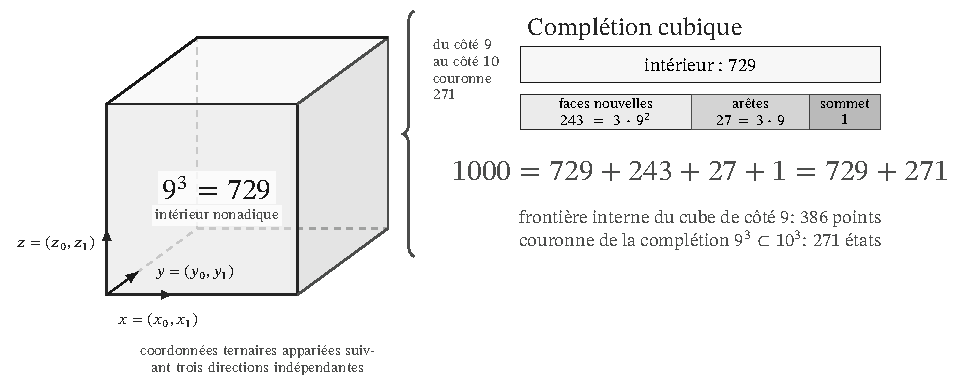
\includegraphics[width=\textwidth]{figures/cubo_emrh_original.pdf}
\caption{Représentation cubique de l'extension de neuf à dix classes par coordonnée. Les strates \(S_1,S_2,S_3\) placent les incidences ajoutées sur les faces, les arêtes et l'apex ; leurs cardinaux forment la couronne de \(271\) éléments. La frontière de \(386\) éléments appartient au cube initial. La perspective géométrique complète la partition de la figure ~\ref{fig:revision-emrh} ; les séparations graphiques ont une fonction schématique.}
\label{fig:completacion-cubo-recuperado}
\end{figure}


\subsubsection{Conservation de l'unité et compatibilité dimensionnelle}

La normalisation ne se limite pas à diviser une identité isolée. En dimension
\(d\), le produit \(\widehat E^d\) porte la mesure uniforme
\(\mu_d(\{x\})=10^{-d}\). La projection coordonnée
\(p_d:\widehat E^{d+1}\to\widehat E^d\) supprime la dernière coordonnée.

\begin{proposition}[Compatibilité projective des mesures normalisées]
Pour tout \(d\geq1\),
\[
 (p_d)_*\mu_{d+1}=\mu_d,
 \qquad \mu_d(\widehat E^d)=1.
\]
La masse de la strate comportant \(r\) coordonnées supplémentaires est
\(\binom dr9^{d-r}/10^d\), et la somme des masses de toutes les strates
vaut un.
\end{proposition}
\begin{proof}
Chaque point de \(\widehat E^d\) possède dix préimages. Leur masse totale est
\(10\,10^{-(d+1)}=10^{-d}\). L'égalité pour tout sous-ensemble
s'obtient en sommant sur ses points. La formule stratifiée provient
du même dénombrement que \eqref{eq:revision-estratos} ; le binôme
\((9+1)^d\) donne la normalisation totale.
\end{proof}

En dimension trois, retirer l'apex laisse une masse \(999/1000\), et
le restituer ajoute \(1/1000\). Renormaliser avant la restitution
définirait une autre mesure : la distinction est pertinente sur le plan opératoire.
En particulier, conservation de la masse probabiliste, conservation des
registres de transport et dissipation thermodynamique sont des affirmations portant sur
des objets différents. La proposition démontre la première et fournit le
support compatible pour étudier la deuxième ; la troisième requiert une
réalisation dynamique et énergétique spécifiée.

La frontière géométrique interne demeure également distincte.
Sur le représentant cartésien \(\{1,\ldots,9\}^3\), retirer
\(\{2,\ldots,8\}^3\) laisse \(386\) points. Cette frontière appartient au
cube initial, tandis que \(\widehat C\setminus C\) appartient à son
extension. La complétion cubique, le développement positionnel en base mille et
la lecture d'incidence exceptionnelle partagent des données du support ;
leurs applications respectives déterminent l'information issue de ces données qu'utilise
chaque représentation.


\subsection{Incidence cubique et réalisation lorentzienne}

La complétion cubique apporte une relation entre intérieur et frontière.
Sa géométrie peut être développée au moyen de l'incidence des six faces
avec les huit sommets. Étiquetons les faces par \((i,\varepsilon)\),
\(i\in\{1,2,3\}\), \(\varepsilon\in\{+1,-1\}\), et les sommets par
\(\nu\in\{+1,-1\}^3\). La matrice d'incidence est
\[
 M_{(i,\varepsilon),\nu}=\mathbf1_{\{\nu_i=\varepsilon\}}.
\]
Soient \(u=(1,\ldots,1)^{\mathsf T}\in\RR^6\), \(R_F\) l'opposition des faces et \(P_u=uu^{\mathsf T}/6\), \(P_-=(I-R_F)/2\).

\begin{proposition}[Quotient d'incidence de dimension quatre]
Le gramien d'incidence satisfait
\[
 MM^{\mathsf T}=12P_u+4P_-.
\]
Ses valeurs propres \(12,4,0\) ont les multiplicités \(1,3,2\).
En conséquence,
\[
 Q_\square=\RR^6/\ker(MM^{\mathsf T})
 \simeq\RR u\oplus E_-,\qquad E_-=\operatorname{im}P_-.
\]
\end{proposition}
\begin{proof}
Une face contient quatre sommets ; deux faces opposées ont une intersection vide, et deux faces distinctes non opposées partagent deux sommets. La matrice \(12P_u+4P_-\) possède précisément ces entrées. L'espace uniforme est de dimension un ; les différences entre faces opposées engendrent un espace de dimension trois, orthogonal à l'espace uniforme. Son complément est de dimension deux et appartient au noyau.
\end{proof}

La décomposition \(1+3\) procède de l'incidence. Le choix temporel
est déclaré au moyen de la forme bilinéaire
\[
 B_\square([x],[y])=\langle x,(P_--P_u)y\rangle.
\]
Elle est bien définie sur le quotient, car les deux projecteurs annulent le
noyau. Dans la base
\[
 t=[u]/\sqrt6,\qquad
 d_i=[e_{i,+}-e_{i,-}]/\sqrt2,
\]
sa matrice est \(\operatorname{diag}(-1,1,1,1)\). Sont ainsi explicités
le domaine, la décomposition et la convention de signe qui produisent
la réalisation de Minkowski. Le gramien positif détermine le quotient ;
l'affectation temporelle détermine la forme indéfinie sur celui-ci.

L'opérateur
\[
 W_\square=\sqrt6P_u+\sqrt2P_-,\qquad
 W_\square e_{i,\varepsilon}=t+\varepsilon d_i
\]
envoie les six étiquettes de face sur des directions nulles, puisque
\(B_\square(t+\varepsilon d_i,t+\varepsilon d_i)=-1+1=0\).
L'inversion d'une direction et l'opposition des faces disposent ainsi
d'une réalisation géométrique concrète.

\subsubsection{Soudure, inversion et subdivision}

La réalisation cellulaire utilise un transport inversible \(U_m(a)\),
qui conserve la forme lorentzienne, entre les fibres aux extrémités d'une
arête duale orientée \(a\), une étiquette
de face \(\lambda_m(a)\) et une orientation \(\sigma_m(a)\).
Avec \(\ell_m=\ell_0/9^m\), l'application de soudure est
\[
 \beta_m(a)=\ell_m\sigma_m(a)
 W_{\square,s(a)}e_{\lambda_m(a)}.
\]
L'inversion compatible satisfait
\[
 \beta_m(\bar a)=-U_m(a)\beta_m(a).
\]
Identifions les fibres de l'origine à deux niveaux consécutifs au moyen de l'isométrie de raffinement déclarée. Si les neuf sous-segments \(a_1,\ldots,a_9\), de niveau \(m+1\), conservent leur étiquette et leur orientation lorsqu'ils sont transportés vers cette fibre commune, alors
\begin{equation}
 \beta_m(a)=\sum_{j=1}^9
 U_{m+1}(a_1\cdots a_{j-1})^{-1}\beta_{m+1}(a_j).
 \label{eq:soldadura-refinamiento}
\end{equation}
Chaque terme transporté équivaut à \(\ell_m/9\) suivant la même
direction nulle, ce qui démontre l'identité. L'hypothèse de
compatibilité détermine quelles subdivisions réalisent ce raffinement.
L'équation réunit direction, échelle et transport, au lieu de limiter
la correspondance géométrique à un dénombrement des dimensions.

Une fois également fixées l’orientation et la forme lorentzienne, la dualité de
Hodge dans \(\Lambda^2Q_\square^*\) satisfait \(\star^2=-I\).
En dimension quatre, le signe est \((-1)^{2(4-2)+1}=-1\).
On obtient une structure complexe réelle sur les deux-formes et,
après complexification, les sous-espaces propres de valeurs \(+i\) et
\(-i\). L’application électromagnétique de ce domaine appartient à
l’article III de la série et utilise la construction électronique de
l’article I avec son couplage déclaré.

\subsection{Compatibilité entre les réductions modulaire et positionnelle}

La base décimale par blocs intervient au moyen d'une division euclidienne
qui conserve simultanément le résidu et le quotient :
\[
 n=1000q+r,\qquad 0\le r<1000.
\]
Puisque \(1000\equiv1\pmod9\) et \(1000\equiv1\pmod3\),
\[
 n\equiv q+r\pmod9,\qquad n\equiv q+r\pmod3.
\]
Par conséquent, la réduction d'un bloc requiert la contribution du
quotient pour restituer la classe de l'entier. Les nombres \(0\) et
\(1000\) ont le même reste modulo \(1000\), mais des classes différentes
modulo \(9\) et modulo \(3\). C'est une raison opératoire de conserver
la mémoire pendant le changement de résolution.

Le raffinement ternaire et la détermination d'un préfixe décimal
peuvent se coordonner au moyen d'un unique résidu entier. Si \(N/3^L\)
est une extrémité de cylindre et \(D/1000^r\) une extrémité décimale, nous définissons
\[
 A=1000^rN-D3^L.
\]
En ajoutant six symboles ternaires, \(N'=729N+\nu\),
\(L'=L+6\), avec \(0\le\nu<729\). Si le préfixe décimal reste
fixe, on obtient
\[
 A'=729A+\nu1000^r.
\]
Si l'on incorpore en outre un bloc décimal \(\delta\), alors \(D'=1000D+\delta\), \(r'=r+1\), et
\begin{equation}
 A'=729000A+\nu1000^{r+1}-729\delta3^L.
 \label{eq:residuo-dos-bases}
\end{equation}
Les deux identités se démontrent en substituant les définitions. La
comparaison des extrémités se réduit ainsi à des opérations entières qui
retiennent la contribution de chaque prolongation. Cette compatibilité
permet de raffiner une région avant d'évaluer sa coordonnée réelle.

% Incorporación al final de extension.tex; no contiene una sección principal.
% Procedencia: RESULTADO_RECUPERADO; explicitación sectorial de las hipótesis.
% Fuentes leídas: monografía Doble proyección holográfica (cantera editorial),
% manuscrito/local/01_tesis_recuperada.tex y
% manuscrito/generated/algebra_holonomica.tex, especialmente §§1--7 y 21.
% Definición rectora de número: manuscrito/flattened/main_autosuficiente.tex,
% secciones que comienzan en líneas 22137 y 23000 de la cantera de 775 páginas.
% No se adopta su presentación global como prueba de todas las flechas TPK.

\subsection{Le nombre comme section compatible et la valeur comme lecture}
\label{hist:seccion}

La distinction entre état et observation permet de préciser quel objet se
prolonge lorsque la résolution augmente. À la profondeur \(n\), soit \(X_n\)
l’ensemble des états admissibles produits par APP--TRIT--TPK. Leurs données
comprennent la position, les feuillets somme et produit, les résidus et quotients, le régime,
l’orientation, la retenue, la phase, la route, la frontière, la mémoire et la survie. Ce ne sont pas
des coordonnées indépendantes : les évaluations arithmétiques et les transports
précédents imposent leurs relations. Un prolongement conserve ces relations
dans chaque antécédent, même s’il ajoute de nouvelles étapes et de nouvelles données de mémoire.
La définition suivante formalise cette arithmétique des histoires au moyen
de ses applications de restriction.

Soient \(r_{m,n}:X_m\to X_n\), pour \(m\geq n\), les restrictions de
profondeur, avec \(r_{n,n}=\operatorname{id}\) et
\(r_{\ell,n}=r_{m,n}\circ r_{\ell,m}\). Chaque restriction conserve le
préfixe et l’information déjà déterminée en lui.

\begin{definition}[Section numérique compatible]
Un nombre HMT est une histoire compatible du système d’états :
\begin{equation}
 x=(x_n)_{n\geq0}\in X_\infty:=\varprojlim_n X_n,
 \qquad r_{m,n}(x_m)=x_n.
 \label{hist:limite-inverso}
\end{equation}
Un lecteur est une opération supplémentaire sur un domaine spécifié de ces
histoires. Un chiffre est une observation finie ; une valeur scalaire est une
évaluation du lecteur. Le couple formé de la section et de son lecteur constitue
une présentation munie d’une lecture, non une redéfinition de l’identité de la section.
\end{definition}

Dans le domaine archimédien \(X_\infty^{\mathrm{Arch}}\), le lecteur associe
à chaque préfixe un cylindre fermé, conserve leur emboîtement et fait tendre
leur diamètre vers zéro. Il détermine ainsi
\begin{equation}
 \operatorname{ev}_{\mathbb R}:X_\infty^{\mathrm{Arch}}\longrightarrow
 \mathbb R,\qquad
 \{\operatorname{ev}_{\mathbb R}(x)\}=\bigcap_n I_n(x).
 \label{hist:evaluacion}
\end{equation}
La construction concrète de ces cylindres et la décision de leurs frontières
sont développées dans la section~\ref{sec:generacion}. La définition
\eqref{hist:limite-inverso} n’affirme pas à elle seule que l’image de
\eqref{hist:evaluacion} soit la droite entière : une affirmation de couverture
requiert son propre théorème. Une égalité de valeurs n’établit pas non plus, sans
résultat d’injectivité, l’égalité de leurs histoires. Cette séparation
permet de parler de précision comme profondeur en conservant la différence
entre l’antécédent arithmétique et sa réalisation scalaire.

\subsection{Composition des histoires et multiplicateur de mémoire}
\label{hist:algebra}

Fixons un secteur d’états à la profondeur \(n\) et une catégorie
\(\mathcal C\) dont les flèches sont leurs histoires admissibles. La composition
s’écrit \(vu=v\circ u\) : on parcourt d’abord \(u\), puis \(v\).
Les pas élémentaires proviennent de la sélection, du transport et de
l’actualisation du TPK. Une fibre tritique locale admet l’écriture
\(\mathbb R[J_x]/(J_x^2+\tau(x)1_x)\), où
\(\tau(x)\in\{+1,0,-1\}\). Le régime et l’orientation appartiennent à
l’état transporté ; une transition entre régimes n’équivaut pas à
l’identification de leurs algèbres quadratiques.

La formulation suivante précise un secteur algébrique de cette composition.
Pour chaque objet \(x\), on se donne une algèbre réelle associative unitaire \(A_x\),
éventuellement non commutative. Pour chaque \(u:x\to y\), on se donne un
homomorphisme unital \(\rho_u:A_x\to A_y\). Nous supposons une action stricte :
\begin{equation}
 \rho_{\operatorname{id}_x}=\operatorname{id}_{A_x},\qquad
 \rho_v\rho_u=\rho_{vu}.
 \label{hist:accion-estricta}
\end{equation}
Pour chaque couple composable \(u:x\to y\), \(v:y\to z\), nous fixons un
multiplicateur central inversible
\(\Omega(v,u)\in Z(A_z)^\times\). On exige la normalisation
\(\Omega(\operatorname{id}_y,u)=\Omega(u,\operatorname{id}_x)=1_y\)
et, pour chaque triplet composable, l’identité
\begin{equation}
 \rho_w\bigl(\Omega(v,u)\bigr)\Omega(w,vu)
   =\Omega(w,v)\Omega(wv,u).
 \label{hist:cociclo}
\end{equation}
Il s’agit d’hypothèses explicites sur les transports et leurs coefficients, non d’une
conséquence du qualificatif holonomique appliqué à la dynamique. Pour appliquer cette présentation
à un secteur TPK, il faut identifier ses \(\rho_u\) et \(\Omega(v,u)\).
Les transitions exprimées par des bimodules exigent la conservation de cette
structure et ne sont pas remplacées par \eqref{hist:accion-estricta}.

L’espace des sommes finies
\[
 \mathcal H(\mathcal C,A,\rho,\Omega)
   =\bigoplus_{u\in\operatorname{Mor}(\mathcal C)} A_{t(u)}T_u
\]
est muni du produit bilinéaire
\begin{equation}
 (aT_v)(bT_u)=a\rho_v(b)\Omega(v,u)T_{vu},
 \label{hist:producto}
\end{equation}
si les flèches sont composables, et de zéro sinon. Ici, \(t(u)\)
désigne l’état terminal. La somme réunit des histoires à coefficients ; le
produit concatène les histoires en conservant le multiplicateur du registre.

\begin{proposition}[Associativité sectorielle à multiplicateur central]
Sous \eqref{hist:accion-estricta} et \eqref{hist:cociclo}, le produit
\eqref{hist:producto} est associatif. Si l’ensemble des objets est fini,
son unité est \(\sum_x1_xT_{\operatorname{id}_x}\).
\end{proposition}
\begin{proof}
Pour \(u:x\to y\), \(v:y\to z\), \(w:z\to t\), soient
\(a\in A_y\), \(b\in A_z\), \(c\in A_t\). Les deux coefficients
de \(T_{wvu}\) sont
\begin{align*}
 ((cT_w)(bT_v))(aT_u):\quad&
 c\rho_w(b)\Omega(w,v)\rho_{wv}(a)\Omega(wv,u),\\
 (cT_w)((bT_v)(aT_u)):\quad&
 c\rho_w(b)\rho_w\rho_v(a)\rho_w(\Omega(v,u))\Omega(w,vu).
\end{align*}
L’action stricte identifie \(\rho_w\rho_v(a)\) à \(\rho_{wv}(a)\).
La centralité de \(\Omega(w,v)\) permet de le déplacer à droite de
ce facteur ; \eqref{hist:cociclo} égalise alors les produits restants.
Les coefficients \(a,b,c\) ne sont pas permutés. Si le triplet n’est pas composable,
les deux parenthésages sont nuls du fait de leurs états initiaux et terminaux.
La bilinéarité achève la preuve. Les identités locales et la
normalisation de \(\Omega\) vérifient l’unité indiquée.
\end{proof}

La retenue du calendrier fournit un exemple effectif. Dans la catégorie
à un objet et de flèches \(C_9\), prenons pour coefficients
\(A=\mathbb R[z,z^{-1}]\), l’action identité et
\[
 \Omega(b,a)=z^{c_0(a,b)},\qquad
 c_0(a,b)=\left\lfloor\frac{a+b}{9}\right\rfloor,
 \quad 0\leq a,b<9.
\]
Les deux sommes de retenues d’un triplet sont
\(\lfloor(a+b+c)/9\rfloor\) ; \eqref{hist:cociclo}
est donc satisfaite. La variable formelle \(z\) enregistre le tour sans
lui attribuer de valeur numérique. Imposer ensuite \(z^{12}=1\) restitue le
registre dodécaphasique du calendrier \eqref{eq:extension108} ; conserver
\(z\) sans cette relation distingue les tours successifs. L’exemple réalise
la mémoire de ce calendrier, sans l’identifier à la totalité de la
mémoire TPK.

\subsection{Double variance du raffinement et conservation de l’unité}
\label{hist:doble-varianza}

La restriction des états prolonge les observables en sens contraire.
Considérons les algèbres de fonctions, munies du produit ponctuel,
\(D_n=\operatorname{Fun}(X_n,\mathbb R)\). La précomposition définit
\begin{equation}
 r_{m,n}^*:D_n\longrightarrow D_m,
 \qquad r_{m,n}^*f=f\circ r_{m,n}.
 \label{hist:precomposicion}
\end{equation}
Ce sont des morphismes unitaux ; ils sont également injectifs lorsque les restrictions
correspondantes sont surjectives. La limite inductive
\(D_{\mathrm{cyl}}=\varinjlim_n(D_n,r_{n+1,n}^*)\) réunit les
observations de profondeur finie. Cette algèbre n’est pas identifiée ici
à l’algèbre entière des routes : prolonger les opérateurs de transport exige
également leurs compatibilités avec le raffinement.

\begin{lemma}[Unité et naturalité de l’évaluation]
Si \(e_x\) est l’indicatrice de \(x\in X_n\), on a
\begin{equation}
 r_{m,n}^*e_x=\sum_{y:\,r_{m,n}(y)=x}e_y,
 \qquad r_{m,n}^*1_n=1_m,
 \label{hist:unidad}
\end{equation}
et, pour tous \(f\in D_n\), \(y\in X_m\),
\[
 \langle r_{m,n}^*f,y\rangle=\langle f,r_{m,n}y\rangle.
\]
Chaque section \(x\in X_\infty\) détermine une évaluation bien définie
\(D_{\mathrm{cyl}}\to\mathbb R\), donnée par \([f]\mapsto f(x_n)\)
pour \(f\in D_n\).
\end{lemma}
\begin{proof}
Les fibres de \(r_{m,n}\) forment une partition de \(X_m\). Leurs
indicatrices sont orthogonales et de somme \(1_m\), ce qui démontre
\eqref{hist:unidad}. La naturalité est la définition de la précomposition.
Enfin, \((r_{m,n}^*f)(x_m)=f(x_n)\), de sorte que deux représentants
compatibles donnent la même évaluation dans la limite inductive.
\end{proof}

L’unité globale est la fonction constante un sur toutes les possibilités ;
la section individuelle sélectionne une histoire compatible. Conserver la
première ne signifie pas immobiliser la seconde. Le raffinement peut augmenter
le nombre d’extensions et la profondeur de chaque histoire en maintenant
l’unité et toutes les évaluations de ses antécédents.

\subsection{Retour de phase, représentation de Weyl et deux lectures}
\label{hist:puente-lecturas}

La loi \eqref{eq:holonomia-memoria} acquiert une réalisation opératorielle
dans la suspension bilatérale qui sera construite dans la
section~\ref{sec:generacion}. Dans celle-ci, \(T\) est l’avancement d’un pas,
\(V_9\) observe la phase nonadique, \(W_\delta\) la phase de rotation et
\(D_M\) le degré de mémoire. En écrivant
\(\widehat\Gamma_9=T^9\) pour le tour dans cette représentation,
les relations de Weyl \eqref{eq:weyl-relojes} impliquent, sur les vecteurs
de support fini,
\begin{equation}
 \begin{aligned}
 V_9\widehat\Gamma_9&=\widehat\Gamma_9V_9,\qquad
 W_\delta\widehat\Gamma_9=e^{2\pi i9\delta}
     \widehat\Gamma_9W_\delta,\\
 [D_M,\widehat\Gamma_9]&=\widehat\Gamma_9.
 \end{aligned}
 \label{hist:tres-retornos}
\end{equation}
La première égalité découle de \(\zeta_9^9=1\) ; la deuxième, de neuf
applications de la covariance de \(W_\delta\) ; la troisième exprime
l’incrément unitaire de mémoire. La phase finie revient, tandis que la
rotation irrationnelle et la mémoire distinguent l’état suivant. Les
caractères et le paramètre \(\delta\) sont réalisés ultérieurement à partir de la
construction numérique spécifiée dans cette section : ils ne sélectionnent pas rétrospectivement
les conditions initiales. Cette représentation décrit les observables et les translations de
la suspension ; elle ne remplace ni toutes les coordonnées ni tous les opérateurs
du TPK.

La double lecture prolonge la même distinction entre histoire et observable.
Dans son domaine archimédien, on applique \eqref{hist:evaluacion} ; dans le
domaine d’incidence calibré, les applications \(Q_n\) de la
section~\ref{exc:doble-lectura} conservent les mots et les repères de
frontière. L’égalité qui y est démontrée,
\(r_{n,m}Q_n=Q_mp_{n,m}\), détermine leur prolongement \(Q_\infty\).
Sur le domaine commun aux deux lectures, on peut considérer conjointement
\(\operatorname{ev}_{\mathbb R}(x)\) et \(Q_\infty(x)\) : la
première retient la valeur ; la seconde, l’incidence transportée que son
codomaine conserve. La section précède les deux. Cette articulation permet
de passer de l’arithmétique des histoires aux constantes et à la lecture
exceptionnelle sans transformer leurs réalisations en nouvelles données initiales.


\clearpage
\section{Génération coinductive de \texorpdfstring{\(\pi,\varphi,e\)}{pi, phi, e} à profondeur arbitraire}
\label{sec:generacion}

L'émission de six blocs est une étape finie de la construction, et non un développement décimal complet. Sa fonction consiste à produire des régions munies de multiplicités, d'orientations et de règles de transport. Le prolongement doit conserver ces données et déterminer une collection compatible de préfixes de longueur arbitraire. Le mot \emph{génération} désigne cette opération ; \emph{généalogie} désigne la reconstruction de ses dépendances. Les deux notions interviennent, mais remplissent des fonctions distinctes.

\subsection{Orbites, régions et caractères de clôture, de propagation et d'auto-échelle}

Sur un mot \(w=(w_1,\ldots,w_6)\), nous définissons
\[
 r(w)=(w_3,w_1,w_2,w_5,w_6,w_4),\qquad
 s(w)=(w_4,w_5,w_6,w_1,w_2,w_3).
\]
On a \(r^3=s^2=I\) et \(srs=r^{-1}\) ; ces permutations réalisent donc le groupe diédral \(D_3\). L'action conserve le catalogue et les multiplicités et commute avec \(\Psi\). Le quotient des \(243\) mots visibles possède \(43\) orbites : trente-huit de cardinal six et cinq de cardinal trois.

La classe de clôture se reconnaît par un prédicat de fibre : ses six orientations ont cinq émissions par mot, une multiplicité totale \(1008\) et une distribution \(432+4\cdot144\). Il existe une seule orbite possédant ces propriétés dans le catalogue. Pour préciser les deux autres sélections, nous écrivons \(f(w)=\#\Psi^{-1}(w)\), \(m(w)=\sum_{U\in\Psi^{-1}(w)}\operatorname{mult}(U)\) et \(\nu(w)=(n_0,n_1,n_2)\). La classe diagonale additive d'une émission est \(d(U)=[i+j]_9\) dans les indices de zéro à huit ; sa signature additive conserve cette classe et l'orientation \(ES\) ou \(NO\). Soit \(\mathcal D(\mathcal O)\) l'ensemble de ces classes pour toutes les émissions sur une orbite.

Parmi les orbites de taille six, le prédicat conjoint
\[
 f(w)=1,\qquad m(w)=144\quad(w\in\mathcal O),\qquad
 \mathcal D(\mathcal O)=\{0,3,6\}
\]
laisse exactement six orbites. Dans ce secteur, le recensement \(\nu=(2,3,1)\), égal à celui de clôture, sélectionne uniquement la propagation ; le recensement \(\nu=(2,2,2)\) sélectionne uniquement l'auto-échelle. Le support diagonal ne peut pas être omis : sans lui, il y a quatre orbites à un seul point équilibrées de multiplicité \(144\), et non une seule. Enfin, l'existence d'une émission avec \(d=6\) et une orientation \(ES\) sélectionne un représentant de chaque orbite et conduit à
\begin{equation}
 w^{\rm cl}=010211,\qquad w^{\rm pr}=201101,\qquad w^{\rm au}=121200.
 \label{eq:palabras-regionales}
\end{equation}
Ces symboles désignent d'abord des régions du catalogue. L'identification scalaire sera démontrée au moyen de leurs lecteurs ; ils ne sont pas choisis parce qu'ils coïncident avec des chiffres d'une constante connue.

Le mot de clôture \(010211\) possède les cinq préimages suivantes :
\begin{center}\small
\begin{tabular}{@{}lll r@{}}\toprule
Émission de six blocs&Signature multiplicative&Rôle&Multiplicité\\\midrule
\(501,614,498,169,272,272\)&\(555555\)&transversal&432\\
\(810,923,870,169,272,272\)&\(339555\)&orientation positive&144\\
\(810,983,810,169,272,272\)&\(393555\)&orientation positive&144\\
\(870,923,810,169,272,272\)&\(933555\)&orientation positive&144\\
\(870,923,810,418,674,521\)&\(933717\)&retour orienté&144\\\bottomrule
\end{tabular}
\end{center}
La multiplicité \(432\) et la signature constante \(555555\) caractérisent la région transversale. Elles n'identifient pas la position centrale \((5,5)\) d'APP. Confondre une signature de six fenêtres avec une position du support éliminerait la distinction entre région numérique et structure électronique.

La microfibre possède en outre une morphologie bipartite précise. Chaque émission est un produit d'une classe de curseur additif et d'une classe multiplicative. Les trois régions positives partagent la même classe additive de dix-huit conditions ; ensemble, elles contiennent trois classes multiplicatives de huit conditions chacune. La région transversale possède un produit \(18\times24\) ; les trois positives réunies, un autre \(18\times24\) ; et le retour, un produit \(18\times8\). La décomposition par émissions comporte cinq parties, tandis que la décomposition en composantes connexes du graphe biparti en comporte trois. Toutes deux conservent les mêmes \(1008\) germes sans réduire la forme à un cardinal.

\subsection{Transport fini et frontière de prolongement}

Les endomorphismes \(L_0,L_1\) de l'espace des mots ternaires agissent avant la réalisation archimédienne. Leur détermination commence par les transitions de l'état arithmétique, et non par la prescription de deux matrices. Si \(U_t\) est l'étape composée de sélection, de transport et de mise à jour, le bloc observé satisfait
\[
 b_j^\chi=\Pi_6(x_j^\chi),\qquad
 x_{j+1}^\chi=U_{9j+9}\cdots U_{9j+1}(x_j^\chi),
 \qquad \chi\in\{\mathrm{cl},\mathrm{pr},\mathrm{au}\}.
\]
On forme six transitions pour chaque régime : deux consécutives dans chacune des trois régions. Les couples de matrices d'origines et de destinations obtenus dans le registre sont
\[
\begin{array}{c|c|c|c}
X_0&Y_0&X_1&Y_1\\\hline
010211&012222&010211&002111\\
012222&010211&002111&110221\\
201101&121221&102011&012222\\
121221&102011&012222&102011\\
121200&112202&121020&010210\\
112202&121020&010210&010200
\end{array}
\]
Chaque chaîne de six chiffres représente une ligne dans \(\FF_3^6\). Puisque \(\det X_0=1\) et \(\det X_1=-1\) dans \(\FF_3\), les équations \(X_aL_a=Y_a\) déterminent de manière unique \(L_a=X_a^{-1}Y_a\). Dans cette coordinatisation par vecteurs-lignes, on obtient
\[
 L_0=\begin{pmatrix}
 2&2&2&1&2&1\\2&1&2&2&1&1\\1&0&0&1&0&2\\
 0&0&1&1&1&0\\2&2&2&0&2&1\\2&1&2&1&0&0
 \end{pmatrix},\quad
 L_1=\begin{pmatrix}
 2&1&2&0&2&2\\1&2&1&1&2&0\\1&2&1&1&1&2\\
 0&1&0&0&2&1\\2&0&2&1&0&1\\0&2&2&2&1&1
 \end{pmatrix}\quad(\bmod3).
\]
Le calendrier \((L_0,L_0,L_1,L_1)\) produit quatre nouveaux blocs de six composantes. Leurs concaténations forment
\[
 w_6\longrightarrow w_{12}\longrightarrow w_{18}
 \longrightarrow w_{24}\longrightarrow w_{30}.
\]
Les sous-indices de \(w\) indiquent la longueur accumulée. La frontière \(R_{36}\) conserve la structure terminale et ouvre la relation de prolongement ; elle n'est pas renommée comme un dernier bloc périodique qui pourrait se répéter indéfiniment.

L'identité \(L=X^{-1}Y\) démontre l'unicité une fois les transitions fixées ; elle ne remplace pas la production de ces transitions par \(U_t\). La provenance de leur registre et l'examen des seize calendriers binaires sont documentés dans le supplément technique. Le calendrier indiqué est le seul de ces seize calendriers qui reproduise conjointement les trois suites de cinq blocs.

\subsection{Cinq régions de clôture et compensation angulaire}

La région de clôture contient une composante transversale et quatre accompagnatrices. Le lecteur symétrique agit dans l'espace de leurs cinq positions au moyen de
\[
 P_5=\frac15\mathbf1\mathbf1^{\mathsf T},\qquad
 \mathbf1=(1,1,1,1,1)^{\mathsf T}.
\]
L'invariance \(P_5\lambda=\lambda\) et la conservation \(\mathbf1^{\mathsf T}\lambda=1\) imposent \(\lambda=\mathbf1/5\). Cette normalisation répartit l'unité entre les positions du lecteur ; elle ne remplace pas les multiplicités des germes \(432,144,144,144,144\) par des fréquences uniformes. La coordinatisation elliptique du lecteur réalise chaque coordonnée par \(1+\lambda_jJ\) ; sa pente est \(\lambda_j\), d'où la pente primitive \(1/5\). La règle qui fait passer d'une coordonnée normalisée à une pente est ainsi explicitée, au lieu d'identifier les deux notions sans application. Le lecteur compose les quatre positions associées selon la loi
\begin{equation}
 a\oplus b=\frac{a+b}{1-ab}.
 \label{eq:suma-pendientes}
\end{equation}
Cette loi s'obtient en multipliant \((1+aJ)(1+bJ)\) dans le régime \(J^2=-I\) et en divisant par sa composante scalaire. La composition des pentes est donc une réalisation de la structure quadratique de TRIT, et non une somme ordinaire de quatre fractions.

\begin{proposition}[Compensateur de la clôture]
La composition de quatre pentes \(1/5\) est \(120/119\). La condition de retour à une pente un détermine un unique compensateur positif de la forme \(1/q\), avec \(q>1\), et donne \(q=239\).
\end{proposition}
\begin{proof}
La première duplication donne \((1/5)\oplus(1/5)=5/12\) ; la seconde, \((5/12)\oplus(5/12)=120/119\). La condition
\[
 \frac{120/119-1/q}{1+(120/119)/q}=1
\]
équivaut à \((120-119)q=120+119\), d'où \(q=239\).
\end{proof}

Le caractère de clôture résultant a pour réalisation
\begin{equation}
 \Pi_{\rm cl}=4\left(4\arctan\frac15-\arctan\frac1{239}\right).
 \label{eq:lector-pi}
\end{equation}
L'identité angulaire de Machin reconnaît \(\Pi_{\rm cl}=\pi\). Le sens de la construction est précis : la pente et le nombre de compositions sont déclarés par le lecteur de la pentafibre ; l'équation de compensation impose \(239\). Une fois ce caractère produit, son évaluation par des séries alternées ne sélectionne pas à nouveau l'orbite des germes.

Pour \(0<x<1\), les sommes alternées
\[
 A_n(x)=\sum_{j=0}^n\frac{(-1)^jx^{2j+1}}{2j+1}
\]
encadrent \(\arctan x\) entre deux troncatures consécutives, dont la différence est \(x^{2n+3}/(2n+3)\). Appliquées aux deux pentes de \eqref{eq:lector-pi}, elles fournissent des extrémités rationnelles d'erreur explicite. La valeur numérique est ainsi calculée comme conséquence du caractère exact, sans introduire de préfixe cible.

\subsection{Lecteur de propagation et normalisation de l'unité}

La région de propagation se réalise au moyen d'une collection formelle \(P_t\in\mathcal A[[t]]\), où \(\mathcal A\) est une algèbre commutative unitaire sur \(\QQ\). Sa composition satisfait \(P_{t+s}=P_tP_s\), d'unité \(P_0=1\), et le transport élémentaire orienté fixe le générateur scalaire \(P'_0=+1\). La condition fixe son signe, et non sa seule grandeur. En écrivant
\[
 P_t=\sum_{n\ge0}a_nt^n,
\]
la normalisation détermine \(a_0=a_1=1\). La comparaison du coefficient de \(s^nt\) dans \(P_{s+t}=P_sP_t\) donne \((n+1)a_{n+1}=a_na_1\) ; de manière équivalente, \(P'_t=P_t\). Ainsi,
\begin{equation}
 (n+1)a_{n+1}=a_n,\qquad a_n=\frac1{n!}.
 \label{eq:propagacion}
\end{equation}
Le caractère en une unité de paramètre est \(\Pi_{\rm pr}=P_1\), reconnu ultérieurement comme \(e\).

La normalisation du générateur importe. La loi de semi-groupe sans cette donnée admettrait \(P_t=e^{ct}\) pour différents \(c\) ; c'est pourquoi on n'omet pas la condition qui fixe l'unité du paramètre dans le lecteur. Cette condition est antérieure à la comparaison décimale et appartient à l'exposition de la règle opératoire, et non au choix d'une valeur expérimentale.

\begin{proposition}[Bornes rationnelles de propagation]
Pour \(n\ge1\), soit \(E_n=\sum_{j=0}^n1/j!\). Alors
\[
 E_n<\Pi_{\rm pr}<E_n+\frac{n+2}{(n+1)(n+1)!}.
\]
\end{proposition}
\begin{proof}
Le premier terme omis est \(1/(n+1)!\). Chaque quotient ultérieur est au plus égal à \(1/(n+2)\). La somme géométrique majorant la queue est
\[
 \frac1{(n+1)!}\frac1{1-1/(n+2)}
 =\frac{n+2}{(n+1)(n+1)!}.
\]
L'inégalité stricte découle de la décroissance des quotients successifs.
\end{proof}

\subsection{Incidence modale et génération de l'auto-échelle}

Le sélecteur tritique produit le cycle \((+1,-1,0)\). Dans les modes \(\Sigma,\Pi\), la règle est \(+1:m\mapsto\Sigma\), \(-1:m\mapsto\Pi\), \(0:m\mapsto m\). Avec fermeture cyclique, le mode observé est \((\Sigma,\Pi,\Pi)\). Ses arêtes sont \(\Sigma\to\Pi\), \(\Pi\to\Pi\) et \(\Pi\to\Sigma\). Son incidence, dans cet ordre des modes, est donc
\begin{equation}
 F_{\rm av}=\begin{pmatrix}0&1\\1&1\end{pmatrix}.
 \label{eq:fav}
\end{equation}
Les quatre entrées s'obtiennent à partir du calendrier, et non d'une équation qui aurait préalablement reçu la valeur de \(\varphi\). La répétition du calendrier donne les dénombrements \(3F_{\rm av},9F_{\rm av},36F_{\rm av}\) aux longueurs neuf, vingt-sept et cent huit. Ces dénombrements ne sont pas les puissances de la matrice.

\begin{theorem}[Caractère positif d'auto-échelle]
L'incidence \eqref{eq:fav} possède un unique rayon propre strictement positif. En le normalisant sous la forme \((1,x)^{\mathsf T}\), sa coordonnée \(x\) satisfait \(x^2-x-1=0\), \(x>0\), et vaut \(\varphi=(1+\sqrt5)/2\).
\end{theorem}
\begin{proof}
L'équation propre donne \(x=\lambda\) et \(1+x=\lambda x\). L'élimination de \(\lambda\) produit le polynôme. Une seule de ses deux racines est positive. Comme \(F_{\rm av}^2\) a toutes ses entrées positives, le rayon positif est unique et simple. L'expression radicale reconnaît la coordonnée obtenue ; elle ne participe pas à la production de \(F_{\rm av}\).
\end{proof}

Avec \(F_0=0,F_1=1,F_{n+1}=F_n+F_{n-1}\), l'incidence induit, pour \(n\geq1\),
\[
 F_{\rm av}^n=\begin{pmatrix}F_{n-1}&F_n\\F_n&F_{n+1}\end{pmatrix}.
\]
Les quotients consécutifs \(F_{n+1}/F_n\) alternent autour de \(\varphi\). L'identité de déterminant
\[
 F_{n+1}^2-F_nF_{n+2}=(-1)^n
\]
donne une largeur exacte \(1/(F_nF_{n+1})\) entre deux quotients consécutifs. Sa croissance rend cet encadrement rationnel arbitrairement petit.

La mesure sur toutes les histoires compatibles ne coïncide pas avec la fréquence des modes du calendrier à trois événements. La fréquence chronologique est \((1/3,2/3)\). La mesure d'entropie maximale de l'enveloppe symbolique définie par \(F_{\rm av}\) se construit à partir de ses vecteurs propres et a pour rapport de poids \(\varphi^{-2}\). Cette dernière intervient dans la lecture surfacique--volumétrique ; elle ne s'obtient pas en remplaçant simplement une fréquence de comptage par une autre.

Une fois les caractères générés, les deux orientations du lecteur
\[
 R(x,y)=\frac{x}{y^2}
\]
fournissent
\begin{equation}
 \rho_A=\frac\pi{\varphi^2},\qquad
 \rho_E=\frac\varphi{\pi^2},\qquad
 \varphi^3\rho_A^2\rho_E=1.
 \label{eq:areal-electron}
\end{equation}
La seconde expression intervient dans l’exposant électronique développé dans l’article I de la série. La première s’obtient également comme limite de la lecture marquée \(\pi F_{n-1}/F_{n+1}\). L’échange des arguments relie les deux, mais ne transforme pas une reparamétrisation de l’équation électronique en une seconde dérivation indépendante de tous ses coefficients.

% Articulación posterior a la generación de pi, phi y e.
% Contenido acumulativo; no reemplaza el desarrollo previo del TRIT.
\subsection{Réalisations exponentielles des coordonnées générées}
\label{euler-trit-articulacion}

Les coordonnées régionales déjà déterminées permettent de reconnaître les
réalisations concrètes de la collection quadratique du TRIT. L'ordre est
essentiel : la construction des régions précède l'évaluation d'une
exponentielle aux paramètres \(\pi\) ou \(2\log\varphi\). Ces expressions
identifient la fonction des coordonnées dans des opérateurs construits à partir
d'APP et du TPK ; elles n'interviennent pas dans la sélection des préfixes qui les produisent.

\subsubsection{Cycle ternaire, transport nilpotent et incidence des feuillets}

La multiplication \(a(r)=4r\) dans \(\mathbb Z/9\mathbb Z\) est d’ordre
\(3\). Sur les unités, elle détermine les orbites \(\{1,4,7\}\) et
\(\{2,8,5\}\). Dans le module d’augmentation de l’une quelconque d’entre elles, formé
des combinaisons entières dont les coefficients ont une somme nulle, la base
\((e_r-e_{4r},e_{4r}-e_{7r})\) donne
\[
 C=\begin{pmatrix}0&-1\\1&-1\end{pmatrix},
 \qquad C^2+C+I=0.
\]
La forme restreinte a pour matrice de Gram
\(\bigl(\begin{smallmatrix}2&-1\\-1&2\end{smallmatrix}\bigr)\).
Dans les évaluations résiduelles modulo \(9\), l’action distingue les feuillets :
\(S(ax,ay)=aS(x,y)\), tandis que \(P(ax,ay)=a^{-1}P(x,y)\).
La réalisation cyclique conserve donc une orientation contragrédiente
entre somme et produit. Les quotients du relèvement entier sont conservés
dans le registre arithmétique correspondant.

Le transport parabolique élémentaire est représenté par
\[
 N=\begin{pmatrix}0&1\\0&0\end{pmatrix}.
\]
L’incidence surfacique--volumique déjà construite dans \eqref{eq:fav} fournit
\[
 F_{\rm av}=\begin{pmatrix}0&1\\1&1\end{pmatrix},
 \qquad A=F_{\rm av}^2=\begin{pmatrix}1&1\\1&2\end{pmatrix}.
\]
Les trois opérateurs agissent dans des espaces réels déclarés : le module
d’augmentation tensorisé avec \(\mathbb R\), le plan du transport nilpotent et
le plan d’incidence modale. Le partage d’une dimension matricielle n’identifie
ni ces espaces ni leurs coordonnées.

\begin{proposition}[Générateurs concrets des trois types]
\label{euler-trit-generadores}
Les opérateurs
\[
 J_{\mathrm e}=\frac{2C+I}{\sqrt3},\qquad
 J_{\mathrm p}=N,\qquad
 J_{\mathrm h}=\frac{2A-3I}{\sqrt5}
\]
satisfont, respectivement,
\[
 J_{\mathrm e}^{\,2}=-I,\qquad
 J_{\mathrm p}^{\,2}=0,\qquad
 J_{\mathrm h}^{\,2}=I.
\]
\end{proposition}
\begin{proof}
La relation de \(C\) implique \((2C+I)^2=-3I\).
La multiplication directe donne \(N^2=0\).
Enfin, \(A\) est de trace \(3\) et de déterminant \(1\), d’où
\(A^2-3A+I=0\) et \((2A-3I)^2=5I\).
\end{proof}

\begin{proposition}[Trois évaluations de l’identité exponentielle]
\label{euler-trit-evaluaciones}
Dans les réalisations précédentes,
\begin{equation}
 \boxed{
 \exp(\pi J_{\mathrm e})+I=0,\qquad
 \exp(J_{\mathrm p})=I+J_{\mathrm p},\qquad
 \exp(2\log\varphi\,J_{\mathrm h})=F_{\rm av}^{\,2}.}
 \label{euler-trit-tres-evaluaciones}
\end{equation}
\end{proposition}
\begin{proof}
La spécialisation elliptique de l’exponentielle tritique donne
\(\cos\pi\,I+\sin\pi\,J_{\mathrm e}=-I\).
La nilpotence élimine exactement les termes de degré au moins \(2\)
dans la deuxième expression. Pour la troisième, \(\varphi^2=\varphi+1\) implique
\[
 \cosh(2\log\varphi)=\frac32,\qquad
 \sinh(2\log\varphi)=\frac{\sqrt5}{2}.
\]
L’exponentielle vaut donc
\(\frac32I+\frac{\sqrt5}{2}J_{\mathrm h}=A\).
\end{proof}

La première égalité représente le demi-tour elliptique ; le tour complet
satisfait \(\exp(2\pi J_{\mathrm e})=I\). La deuxième maintient un terme
linéaire non nul : le régime parabolique exprime un transport, et non une absence
d'évolution. La troisième réalise une avancée hyperbolique unimodulaire. Ses
valeurs propres sont \(\varphi^2\) et \(\varphi^{-2}\) ; une direction se dilate et
l'autre se contracte en conservant le déterminant. Les trois évaluations
emploient des paramètres distincts d'une collection exponentielle commune.

Dans cette collection, \(e\) intervient par l'évaluation scalaire
\(\exp(I)=eI\) et la loi \(\exp(sI)\exp(tI)=\exp((s+t)I)\).
Son rôle ne se limite pas au type parabolique. La coordonnée \(e\), obtenue
auparavant à partir de sa région, est reconnue ici comme l'évaluation en l'unité
de l'exponentielle ; cette identité ne remplace pas sa généalogie coinductive.

\subsubsection{Résolution polynomiale des régimes}

Les trois réalisations admettent une présentation compacte sur la somme
directe de leurs espaces. On définit
\[
 \mathbb J=J_{\mathrm e}\oplus J_{\mathrm p}\oplus J_{\mathrm h},
 \qquad Q=\mathbb J^2.
\]
Les relations précédentes impliquent
\[
 \mathbb J^6=\mathbb J^2,\qquad Q^3=Q.
\]
L’emploi de \(Q\) maintient ce carré opératoriel distinct du registre
dodécaphasique \(K\).

\begin{proposition}[Projecteurs polynomiaux de régime]
\label{euler-trit-proyectores}
Les applications
\[
 p_{\mathrm e}=\frac{Q^2-Q}{2},\qquad
 p_{\mathrm p}=I-Q^2,\qquad
 p_{\mathrm h}=\frac{Q^2+Q}{2}
\]
sont des idempotents mutuellement orthogonaux, de somme \(I\), qui restituent les trois
termes de la somme directe représentant les régimes.
\end{proposition}
\begin{proof}
Les trois polynômes prennent les valeurs \((1,0,0)\), \((0,1,0)\) et
\((0,0,1)\) aux points \(-1,0,+1\), respectivement. Les différences
entre leurs carrés et eux-mêmes, ainsi que leurs produits croisés, sont
des multiples de \(X^3-X\). Substituer \(Q\), qui annule ce polynôme, démontre
les identités. Dans les trois blocs, \(Q\) agit comme \(-I,0,I\).
\end{proof}

On obtient ainsi
\begin{align}
 \exp(t\mathbb J)
 ={}&p_{\mathrm e}(\cos t\,I+\sin t\,\mathbb J)
   +p_{\mathrm p}(I+t\mathbb J)\notag\\
   &+p_{\mathrm h}(\cosh t\,I+\sinh t\,\mathbb J).
 \label{euler-trit-exponencial-total}
\end{align}
Chaque terme conserve sa relation quadratique et la conjugaison inverse
son évolution. La représentation totale réunit les trois régimes, mais ne
définit pas à elle seule un opérateur de transition entre eux. Une telle transition
requiert les applications de transport du TPK avec leurs domaines, leur orientation et
leur mémoire. L’articulation exponentielle permet de reconnaître leurs types sans
remplacer cette dynamique par une identification des fibres.

% PROCEDENCIA FOCAL (no impresa)
% Resultado recuperado: tres generadores y tres evaluaciones exponenciales.
% Propietario completo:
% BASE/manuscrito/sections/hmt/09b_algebras_cuadraticas.tex:289-516.
% Antecedente causal de C y acción contragrediente:
% BASE/manuscrito/sections/hmt/03d_esqueleto_ciclotomico_app.tex:13-47,145-246.
% Los tres tipos y la orientación están en:
% BASE/manuscrito/sections/hmt/02_trit_geometrias.tex:83-196.
% Resolución polinómica recuperada:
% output/INVESTIGACION_HOLONOMIA_NONADICA_CRISTAL_APERIODICO_20260903/
% ALGEBRA_HOLONOMICA_UNIVERSAL_Y_EULER_TRITICO.md, secciones 8-11 y 22.
% Los cuatro propietarios se leyeron completos. BASE designa:
% /Users/ruben/Documents/HMT2/
% EL_CIERRE_HOLOGRAFICO_DEL_INFINITO_SUCESOR_102_CAPITULOS_2026-08-28_EN_TRABAJO/
% No se incorpora la identidad P9(alpha)=delta del documento especializado:
% esa identificación no pertenece a este bloque.
% Tampoco se identifica una dirección nilpotente con la vacancia electrónica,
% ni se presume una representación global del transporte por la suma directa.
% COMPROBACIONES: Python estándar, enteros y Fraction.
% C^2+C+I=0; (2C+I)^2=-3I; N^2=0; (2Fav^2-3I)^2=5I.
% 81 pares de residuos verifican las dos acciones contragredientes.
% Los 3 proyectores se verificaron en Q=-1,0,+1; prueba general en texto.
% 6 labels únicos y entornos equilibrados. Sin compilación.


\subsection{Cylindres compatibles et profondeur arbitraire}

La réalisation d'un bloc ternaire \(b=(b_1,\ldots,b_6)\) est l'entier
\[
 \nu(b)=\sum_{j=1}^6b_j3^{6-j}\in\{0,\ldots,728\}.
\]
Une suite de blocs définit des préfixes entiers par \(N_{n+1}=729N_n+\nu(b_{n+1})\), en commençant en \(N_0=m\), où \(m\) est la partie entière déterminée par le lecteur. Les fourchettes précédentes situent les caractères de clôture, de propagation et d'auto-échelle dans \((3,4)\), \((2,3)\) et \((1,2)\), respectivement ; leurs valeurs initiales sont donc \(m=3,2,1\). Les blocs suivants raffinent la partie fractionnaire. Le cylindre correspondant est
\begin{equation}
 I_n=\left[\frac{N_n}{729^n},\frac{N_n+1}{729^n}\right],
 \qquad |I_n|=729^{-n}.
 \label{eq:cilindro}
\end{equation}
La convention semi-ouverte est utilisée pour sélectionner un représentant lorsqu'une valeur tombe sur une frontière. Pour le passage à la limite, on utilise les fermetures de ces intervalles et on identifie les deux développements de frontière équivalents. Cette précision empêche de supposer que toute intersection d'intervalles semi-ouverts emboîtés est automatiquement non vide.

\begin{theorem}[Détermination de la réalisation scalaire]
Une histoire de blocs compatible détermine une unique limite des extrémités gauches de \eqref{eq:cilindro}. Si un caractère exact dispose d'encadrements rationnels de largeur arbitrairement petite et se sépare de la frontière de chaque cylindre décimal examiné, chaque préfixe décimal de longueur finie est déterminé après un calcul fini. Les préfixes ainsi obtenus sont compatibles entre eux.
\end{theorem}
\begin{proof}
L'extension d'un bloc conserve le préfixe précédent par division euclidienne. Les cylindres fermés sont emboîtés et leur diamètre tend vers zéro ; leurs extrémités gauches forment une suite de Cauchy et possèdent une unique limite. Pour une longueur décimale fixée, une valeur séparée des frontières de la partition possède une distance positive à celles-ci. Une fourchette suffisamment étroite est contenue dans une unique cellule et détermine son préfixe. L'unicité de la cellule et l'emboîtement des partitions prouvent la compatibilité par troncature. Aux points à développement terminal, il faut ajouter la décision exacte de frontière et sa convention de représentation ; cette décision ne se déduit pas d'une largeur numérique seule.
\end{proof}

Les caractères de clôture, de propagation et d’auto-échelle possèdent les encadrements précédents. Après leur reconnaissance, l’irrationalité de \(\pi,e,\varphi\) garantit leur séparation des frontières rationnelles de toute précision décimale finie. La profondeur arbitraire signifie \emph{pour tout horizon fini, il existe un calcul qui détermine son préfixe} ; elle n’exige pas qu’une machine finie stocke en une seule fois une quantité infinie de chiffres. L’objet mathématique est la famille compatible complète, et une exécution en produit une projection finie.

\subsection{Involution spéculaire et synchronisation des régions}

La connexion nonadique transporte conjointement les trois caractères. Dans la coordinatisation de la neuvième phase, l'axe d'auto-échelle et la somme ternaire de clôture et de propagation restent fixés sous l'échange spéculaire. L'inversion hélicoïdale change le sens du transport ; la réflexion des deux canaux change leur orientation relative. Ce sont des involutions différentes, bien qu'elles agissent sur le même système de trajectoires.

Les coïncidences de recensement illustrent cette coordination :
\begin{center}
\begin{tabular}{@{}c rrr l@{}}\toprule
Phase&\(N_\pi\)&\(N_e\)&\(N_\varphi\)&Égalité des dénombrements\\\midrule
4&207&207&122&\(N_\pi=N_e\)\\
5&39&151&151&\(N_e=N_\varphi\)\\
6&110&110&69&\(N_\pi=N_e\)\\
7&81&29&81&\(N_\varphi=N_\pi\)\\
8&59&59&59&synchronisation triple\\
9&43&43&43&synchronisation triple\\\bottomrule
\end{tabular}
\end{center}
Ces entiers comptent des coordonnées compatibles des régions. Ils n'affirment pas une égalité entre \(\pi\), \(e\) et \(\varphi\) en tant que nombres réels. Si
\[
 \partial(a,b,c)=(a-b,b-c,c-a),
\]
son image appartient au réseau \(A_2=\{(u,v,w)\in\ZZ^3:u+v+w=0\}\). Aux phases huit et neuf, la composante relative s'annule, mais la composante diagonale passe de \((59,59,59)\) à \((43,43,43)\). La synchronisation relative coexiste avec un déplacement de \(-16\) par canal. La fermeture qui conduira à \(\alpha\) doit conserver les deux informations : coïncidence relative et évolution de la mémoire.

\subsection{Suspension hélicoïdale sturmienne}

La relation entre les bases neuf et dix de la complétion définit le paramètre adimensionnel
\begin{equation}
 \delta=\frac{\log(10/9)}{\log10}.
 \label{eq:delta-sturm}
\end{equation}
Elle ne s'obtient pas à partir d'une constante physique cible. C'est l'échelle logarithmique relative de deux bases déjà présentes dans la construction. Son emploi comme lecture symbolique du raffinement a une conséquence exacte.

\begin{lemma}[Irrationalité de la pente]
Le nombre \(\delta\) est irrationnel.
\end{lemma}
\begin{proof}
Si \(\delta=p/q\), \(q>0\), alors \((10/9)^q=10^p\) et \(9^q=10^{q-p}\). La factorisation du premier membre contient le nombre premier trois et celle du second uniquement les nombres premiers deux et cinq. L'égalité est impossible.
\end{proof}

Le mot mécanique inférieur, d'ordonnée à l'origine \(\theta\), est
\[
 z_n(\theta)=\lfloor(n+1)\delta+\theta\rfloor-\lfloor n\delta+\theta\rfloor\in\{0,1\}.
\]
On l'obtient en observant la rotation \(\theta\mapsto\theta+\delta\pmod1\) au moyen de l'intervalle \([1-\delta,1)\). La suite d'événements a pour densité \(\delta\), et la somme sur toute fenêtre de longueur \(L\) vaut \(\lfloor L\delta\rfloor\) ou \(\lceil L\delta\rceil\). Puisque \(21<1/\delta<22\), les séparations entre événements sont vingt et un ou vingt-deux. Le mot qui indique quels sont les intervalles courts est un autre mot mécanique de pente \(\sigma=22-1/\delta\) ; ses événements sont séparés par six ou sept intervalles primaires. La seconde échelle est induite par la première et n'est pas un second paramètre libre.

% Desarrollo reunido de DESARROLLO_MATEMATICO, apartados 38--40 y 50.
\subsubsection{Indice de capacité, lacunes et induction du régime tritique}
\label{vac-capacidad-trit}

La suite des lacunes est liée au raffinement par une
identité d'incréments. Pour la montrer, on fixe l'origine de phase
\(\theta=0\). Soient
\[
 \rho=\log_{10}9=1-\delta,\qquad
 \mathcal C_t=\lfloor(t+1)\rho\rfloor\quad(t\geq0).
\]
L'indice \(\mathcal C_t\) exprime la capacité décimale du raffinement
dans la normalisation qui compare un bloc ternaire de \(6\) positions,
avec \(729\) possibilités, et un bloc décimal de \(3\) positions, avec
\(1000\) possibilités. En effet,
\(\log_{1000}729=\log_{10}9=\rho\). La lettre \(K\) est réservée au
registre dodécaphasique qui sera construit ultérieurement.

\begin{proposition}[Complémentarité de la capacité et de la lacune]
\label{prop:capacidad-vacancia}
Pour \(t\geq1\),
\begin{equation}
 \mathcal C_t-\mathcal C_{t-1}=1-z_t(0).
 \label{eq:capacidad-vacancia}
\end{equation}
Par conséquent, si \(0\leq a<b\),
\[
 \mathcal C_b-\mathcal C_a+
 \sum_{t=a+1}^{b}z_t(0)=b-a.
\]
\end{proposition}
\begin{proof}
L'irrationalité de \(\delta\) donne
\[
 \mathcal C_t
 =t+1-\lceil(t+1)\delta\rceil
 =t-\lfloor(t+1)\delta\rfloor.
\]
La soustraction de deux termes consécutifs produit
\eqref{eq:capacidad-vacancia}. La somme sur l'intervalle est télescopique.
\end{proof}

Chaque transition augmente d'une unité le compteur des blocs. Si
\(z_t=0\), la capacité augmente également ; si \(z_t=1\), la capacité se
maintient tandis qu'une transition est incorporée à l'histoire. La lacune
est ici un événement de rétention de capacité, de position et
d'antécédent déterminés. Le bilan précédent conserve exactement la
longueur entre capacité acquise et lacunes enregistrées. La phase
observée \(g_t^{\rm cap}=[\mathcal C_t]_9\) vérifie
\[
 g_t^{\rm cap}-g_{t-1}^{\rm cap}\equiv1-z_t\pmod9.
\]
Cette phase de capacité et la phase chronologique \([t]_9\) sont deux
observations différentes. Une rétention locale de capacité et un tour
complet de l'holonomie ont des mécanismes distincts, bien que les deux
permettent de conserver l'observation de phase avec modification de l'état.

La relation avec TRIT peut se suivre dans les positions mêmes des lacunes.
Pour \(j\geq1\), définissons
\[
 p_j=\left\lfloor\frac j\delta\right\rfloor,\qquad
 v_j=\mathcal C_{p_j},\qquad h_j=p_{j+1}-p_j.
\]
L'inégalité \(p_j\delta<j<(p_j+1)\delta\) identifie \(p_j\)
comme la position de l'événement \(j\). Comme \(0<\delta<1\), elle donne aussi
\(\lfloor(p_j+1)\delta\rfloor=j\), et par conséquent
\[
 v_j=p_j-j,\qquad
 v_{j+1}-v_j=h_j-1.
\]
Si \(s_j=22-h_j\), alors \(s_j\in\{0,1\}\) et
\begin{equation}
 [v_{j+1}]_3=[v_j-s_j]_3.
 \label{eq:vacancia-regimen}
\end{equation}
Un intervalle de longueur \(22\) conserve la classe ; un intervalle de longueur
\(21\) la décale d'une unité dans le sens négatif. Le sélecteur canonique
s'applique à la phase positive \(r_j=1+[v_j]_9\) :
\[
 \tau_j=M_{\rm ph}(r_j).
\]
Un régime tritique est ainsi déterminé par l'indice de capacité
retenu à chaque événement, en plus du codage binaire de la lacune.

Les positions des intervalles courts forment le codage mécanique
induit de pente \(22-1/\delta\). Leurs espacements \(6\) et \(7\)
déterminent les longueurs des plateaux de la classe \([v_j]_3\), une
fois l'origine et la convention des extrémités fixées. Les premières classes
sont \(2\) pendant \(6\) événements, \(1\) pendant \(7\) et \(0\) pendant
\(7\) ; le premier segment de \(6\) est la restriction initiale d'un plateau.
Leurs signatures parcourent \(0,-1,+1\). Les équations
\eqref{eq:capacidad-vacancia} et \eqref{eq:vacancia-regimen} explicitent le
lien entre raffinement, lacunes et sélection du régime. La lecture
quadratique de TRIT réalise ensuite ces types au moyen de leurs générateurs
respectifs ; l'événement temporel et sa représentation géométrique
conservent ainsi une dépendance identifiable.

L'inversion de l'indice monotone fournit une autre observation utile :
\[
 \mathcal T(k)=\min\{t:\mathcal C_t=k\}
   =\left\lceil\frac k\rho\right\rceil-1\qquad(k\geq1).
\]
Si \(\sigma=\rho^{-1}-1\), le nombre de blocs nécessaires pour acquérir
\(m\) unités de capacité est
\[
 \mathcal T(k+m)-\mathcal T(k)
 =m+\lceil(k+m)\sigma\rceil-\lceil k\sigma\rceil
 \in\{m+\lfloor m\sigma\rfloor,m+\lceil m\sigma\rceil\}.
\]
En particulier, \(9\) unités de capacité nécessitent \(9\) ou \(10\)
blocs. La période d'une phase finie reste exacte, tandis que le
temps de retour mesuré par l'autre indice admet deux valeurs. Cette
distinction fait partie de la dynamique du raffinement et ne constitue pas une correction
de ses valeurs numériques a posteriori.

\begin{proposition}[Renouvellement tritique et capacité marquée]
\label{v:prop:renovacion-capacidad-24}
Soit $K_{\rm ph}$ la représentation de mémoire réduite postérieure à
l’holonomie $\Gamma_9$, et soit $Q(u,r)=(u,[r]_3)$ le quotient de phase
$C_9\to C_3$. Dans chaque bloc de trois régimes, les espérances conditionnelles
$I,E_+,E_\times$ satisfont
\[
 \bar K^3=E_+E_\times=:\Pi,\qquad
 \operatorname{rank}(I,E_+,E_\times,\Pi)=(468,26,18,1).
\]
Si $a_t=\mathcal C_{t+1}-\mathcal C_t$ et
$\mathcal R_t=K_{\rm ph}^{a_t}$, le transport élargi
\[
 (t,\mathcal C_t,v_t)\longmapsto
 (t+1,\mathcal C_t+a_t,v_t+1-a_t)
\]
conserve $t=\mathcal C_t+v_t$. Depuis le premier événement $p_1=21$, le
premier instant où la composition cesse de dépendre du microétat
initial est $T_{\rm ren}=24$, et
\begin{equation}
 (\mathcal C_{p_1},T_{\rm ren},T_{\rm ren}+1,
   \mathcal C_{T_{\rm ren}})=(20,24,25,23).
 \label{v:eq:tupla-renovacion-capacidad}
\end{equation}
La composition directe a les rangs $468\to26\to1$ ; la conjuguée,
$468\to18\to1$.
\end{proposition}
\begin{proof}
Le quotient fort s’obtient en sommant le noyau sur chaque fibre de $Q$.
En trois phases, chaque espérance apparaît une fois et celles-ci sont idempotentes,
autoadjointes et commutatives ; leurs rangs tensoriels donnent les quatre entiers.
Les accroissements de capacité entre $21$ et $24$ appliquent
$I,E_+,E_\times$, de sorte que la première composition de rang un se produit
en $24$. La lecture conjuguée inverse l’ordre des deux espérances et
conserve le même produit final.
\end{proof}

Le retour du régime n’est pas une réinitialisation de l’état : le quotient et la mémoire
continuent d’avancer. Pour les sections marquées ultérieures, on emploie la
règle de localisation
\[
 s_j=\min\{t\ge24:\mathcal C_t=23+3j\},
\]
qui conserve le seuil $23$, le résidu tritique et le quotient illimité.


\begin{theorem}[Complexité des lectures de phase]
Pour \(m\ge1\), le mot mécanique a une complexité factorielle \(p(m)=m+1\). En conservant la phase \(n\bmod9\), la complexité est \(p_9(m)=9(m+1)\) ; en conservant seulement sa classe ternaire, elle est \(p_3(m)=3(m+1)\). Les trois entropies topologiques sont nulles.
\end{theorem}
\begin{proof}
Les prédécesseurs des deux extrémités de l'intervalle de codage forment, pour les facteurs de longueur \(m\), \(m+1\) points distincts du cercle : la coïncidence entre extrémités translatées élimine les doublons et l'irrationalité empêche toute coïncidence supplémentaire. Ces points déterminent \(m+1\) intervalles à itinéraires constants et distincts. Toute orbite irrationnelle visite chaque intervalle, d'où \(p(m)=m+1\).

Une phase modulo neuf étant fixée, les positions de cette phase parcourent une rotation de pas \(9\delta\), également irrationnel. Par densité, tous les facteurs apparaissent dans chaque phase, et la première coordonnée distingue leurs neuf copies. Le même argument avec le pas \(3\delta\) donne trois copies après réduction ternaire. Enfin, \(m^{-1}\log(c(m+1))\to0\) pour \(c=1,3,9\).
\end{proof}

Le produit de phases \(C_9\times\mathbb T\), translaté par \((1,\delta)\), possède des caractères de fréquence
\[
 \frac a9+k\delta\pmod1,\qquad a\in\ZZ/9\ZZ,\ k\in\ZZ.
\]
Le module spectral n'est pas \(\log10\) : c'est le module additif engendré par \(1/9\) et \(\delta\), modulo les entiers. Le facteur \(\log10\) appartient à la normalisation de \eqref{eq:delta-sturm}.

Une présentation opératorielle rend la mémoire explicite. Dans \(\ell^2(\ZZ)\), soient \(T|n\rangle=|n+1\rangle\), \(V_9|n\rangle=\zeta_9^n|n\rangle\), \(W_\delta|n\rangle=e^{2\pi i n\delta}|n\rangle\) et \(D_M|n\rangle=\lfloor n/9\rfloor|n\rangle\). Sur les vecteurs à support fini,
\begin{equation}
 V_9T=\zeta_9TV_9,\qquad
 W_\delta T=e^{2\pi i\delta}TW_\delta,\qquad
 [D_M,T^9]=T^9.
 \label{eq:weyl-relojes}
\end{equation}
Les deux premières relations sont des covariances de Weyl ; la troisième exprime qu'un tour nonadique augmente le degré de mémoire. La rotation de base est abélienne, tandis que l'algèbre des observables et des translations ne l'est pas. L'inversion \(|n\rangle\mapsto|-n\rangle\) conjugue l'avancée avec le recul. Cette réalisation fournit une suspension hélicoïdale apériodique à retour fini de phase, et non un mot périodique de longueur neuf.

\begin{figure}[htbp]
\centering
\begin{tikzpicture}[x=1cm,y=1cm,>=Latex,font=\small]
\begin{scope}[xshift=1.8cm,yshift=.3cm]
\draw[->,gray] (0,-.5)--(0,3.65) node[above] {\(n/9\)};
\foreach \k in {0,1,2,3}{
 \draw[gray!60,dashed] (-1.1,\k)--(1.1,\k);
 \node[left,font=\scriptsize] at (-1.1,\k){\(\k\)};
}
\draw[black,line width=.65pt,domain=0:27,samples=260,smooth,variable=\n]
 plot ({cos(40*\n)},{\n/9+.14*sin(40*\n)});
\foreach \n in {0,...,27}{
 \fill ({cos(40*\n)},{\n/9+.14*sin(40*\n)}) circle (.026);
}
\foreach \k in {0,1,2,3}{\fill (1,\k) circle (.045);}
\node[align=center,text width=3.3cm,font=\scriptsize] at (0,-1.02)
 {Même phase en \(n=0,9,18,27\) ;\\degré de mémoire distinct.};
\end{scope}
\begin{scope}[xshift=4.2cm,yshift=.5cm]
\node[anchor=west] at (0,3.1){\(z_n(0)=\lfloor(n+1)\delta\rfloor-\lfloor n\delta\rfloor\)};
\draw[->] (0,1.7)--(9,1.7) node[right]{\(n\)};
\foreach \n in {21,43,65,87,109,131,152,174,196,218}{
 \draw[line width=.6pt] ({\n*.039},1.7)--({\n*.039},2.25);
 \fill ({\n*.039},2.25) circle (.033);
 \node[below,font=\tiny] at ({\n*.039},1.7){\n};
}
\foreach \a/\b/\g in {21/43/22,43/65/22,65/87/22,87/109/22,109/131/22,131/152/21,152/174/22,174/196/22,196/218/22}{
 \node[font=\scriptsize] at ({(\a+\b)*.0195},2.55){\g};
}
\node[anchor=west,align=left,text width=8.3cm] at (0,.55)
 {Le codage irrationnel détermine les intervalles entre événements. Le retour de la phase nonadique ne transforme pas cette suite en un mot périodique.};
\end{scope}
\end{tikzpicture}
\caption{Représentations complémentaires du transport. À gauche, projection de l'hélice \((\cos(2\pi n/9),\sin(2\pi n/9),n/9)\) : l'avancée de neuf pas retrouve la phase et augmente la hauteur. À droite, les dix premiers événements du mot inférieur pour \(\delta=\log_{10}(10/9)\), avec des espacements exacts de \(21\) ou \(22\). La représentation hélicoïdale n'introduit pas de métrique physique supplémentaire.}
\label{fig:holonomia-esturmiana}
\end{figure}


Pour ce dénombrement, nous fixons l'intercept \(\theta=0\) et les extrémités cumulées \((N_0,\ldots,N_4)=(0,729,972,999,1000)\), correspondant à l'ordre cubique \((729,243,27,1)\). Les dénombrements inférieurs sont \(\lfloor N_j\delta\rfloor-\lfloor N_{j-1}\delta\rfloor\) et donnent \((33,11,1,0)\). Les supérieurs sont \(\lceil N_j\delta\rceil-\lceil N_{j-1}\delta\rceil\), avec la même frontière initiale nulle, et donnent \((34,11,1,0)\). Ces valeurs dépendent de l'intercept et de l'ordre des strates ; elles ne sont pas affirmées pour une phase initiale arbitraire. Leurs totaux sont quarante-cinq et quarante-six. L'incrément correspond à une unique unité de frontière, située dans la première strate de cette partition ordonnée. Les nombres trente-quatre et onze apparaissent ainsi dans un même dénombrement antérieur à toute coordinatisation d'unités ; les identifier à des exposants physiques exige en outre la dérivation dimensionnelle correspondante.

La dénomination \emph{cristal apériodique} est employée ici pour cet ordre symbolique, dont la complexité, le spectre et le retour sont spécifiés. L'entropie topologique nulle n'équivaut pas à elle seule à une dissipation physique nulle : une réalisation thermodynamique exige une dynamique énergétique et une opération d'effacement définies. De même, cette lecture sturmienne ne remplace pas tous les opérateurs du TPK et ne démontre pas à elle seule la périodicité ou l'apériodicité de la sortie complète de \(\alpha\). Sa fonction est d'expliciter une structure d'ordre que le simple retour du calendrier ne décrit pas.

% Adición acumulativa. Insertar después de la suspensión esturmiana existente.
% Conservar íntegro el texto y la figura fig:holonomia-esturmiana.
\subsection{Connexion nonadique, holonomie et représentation monodromique}
\label{mono-ampl:conexion}

La structure régionale requiert de distinguer le transport qui produit une
histoire, l'observation de sa phase et la représentation de ses retours.
APP fournit les deux évaluations arithmétiques avec résidu et quotient ; TRIT
détermine le régime et l'orientation ; le Topological Phase Kernel compose
sélection, transport et mise à jour. Les conditions initiales de
cardinal \(104\,976\), leur catalogue de \(468\) émissions et les \(243\)
mots visibles dans l'espace ambiant de \(729\) éléments appartiennent à des étapes
distinctes de cette construction. La chaîne
\[
 w_6\longrightarrow w_{12}\longrightarrow w_{18}
 \longrightarrow w_{24}\longrightarrow w_{30}
 \longrightarrow R_{36}\longrightarrow G_9
\]
conduit à une connexion conjointe sur les trois régions. Ses neuf phases
sont des positions d’un même transport, et les coordonnées régionales
\(\pi,\varphi,e\), avec la détermination dodécaphasique de \(\alpha\),
procèdent de leurs lectures compatibles, développées dans les
sections~\ref{sec:generacion}, \ref{sec:k-registro} et
\ref{subsec:alpha-limite-dos-vias}.

À l'indice de prolongement \(k\), une coordinatisation de l'état conserve
\[
 \widehat x_k=(B_k,C_k,p_k,c_k,\Sigma_k,W_k,g_k,m_k).
\]
Ici, \(B_k\) réunit les trois blocs régionaux, \(C_k\) est le cylindre,
\(p_k\) le préfixe, \(c_k\) le registre de retenue arithmétique, \(\Sigma_k\) la signature
de frontière et \(W_k\) l'information incidencielle. La phase est
\(g_k=1+[(k-1)]_9\) ; \(m_k\) compte les tours complets. La réduction
\(\beta_k=[m_k]_{12}\) conserve la position dodécaphasique, tandis que
l'entier \(m_k\) distingue ses tours successifs.

\begin{definition}[Transport d'un tour nonadique]
\label{mono-ampl:def-vuelta}
Soient \(\mathcal R_k\subseteq\widehat X_k\times\widehat X_{k+1}\)
les relations d'extension admissible du TPK. La réalisation de
l'holonomie au niveau \(k\) est la composition relationnelle
\[
 \Gamma_{9,k}=\mathcal R_{k+8}\circ\cdots\circ\mathcal R_k.
\]
Pour \(s\geq1\), son prolongement à \(s\) tours est
\[
 \Gamma_{9s,k}=
 \Gamma_{9,k+9(s-1)}\circ\cdots\circ\Gamma_{9,k}.
\]
\end{definition}

La formulation relationnelle conserve les continuations admissibles. Sur
une histoire individualisée, chaque flèche mène à l'état effectivement
prolongé ; le bloc visible isolé peut encore admettre plusieurs
continuations. Cette différence est précisément la fonction de la mémoire et
des conditions de frontière dans la détermination de la trajectoire.

\begin{proposition}[Itération du retour et mémoire accumulée]
\label{mono-ampl:vueltas}
Dans toute composition admissible de \(s\) tours,
\[
 g_{k+9s}=g_k,\qquad m_{k+9s}=m_k+s,\qquad
 \beta_{k+9s}=\beta_k+s\pmod{12}.
\]
\end{proposition}
\begin{proof}
La règle d'un tour conserve la phase et incrémente le compteur d'une
unité. Son application à l'état déjà transporté répète exactement ces
deux opérations. La récurrence donne les deux premières égalités ; réduire la
seconde modulo \(12\) donne la troisième.
\end{proof}

Le compteur fournit ainsi un témoin entier de la différence entre les
tours. Après \(12\) tours, le couple des phases finies est rétabli, mais
le compteur augmente de \(12\). L'extension non scindée
\eqref{eq:extension108} exprime la composition du calendrier par son
cocycle ; la trajectoire conserve en outre le relèvement entier de cette donnée.
La conservation signifie ici le transport des contributions antérieures,
et non l'immobilité de toutes les coordonnées.

\subsubsection{Représentation bilatérale de l'indice de retour}

La réalisation géométrique du graphe cyclique admet une représentation
opératorielle particulièrement simple. Nous numérotons ici les phases de \(0\) à
\(8\), par un déplacement de l'origine par rapport à \(g_k\), et
écrivons \(k=9m+r\), avec \(0\leq r<9\), sur la droite entière
qui recouvre le cycle des phases. Sur
\(\mathcal H_{\rm ind}=\ell^2(\mathbb Z)\), la base
\(|k\rangle=|r,m\rangle\) permet d'exprimer le déplacement unitaire
\[
 T|r,m\rangle=
 \begin{cases}
 |r+1,m\rangle,&r<8,\\
 |0,m+1\rangle,&r=8.
 \end{cases}
\]
L'inverse réduit \(r\) d'une unité lorsque \(r>0\), et envoie
\(|0,m\rangle\) sur \(|8,m-1\rangle\). Le passage par l'origine de phase
incorpore donc l'unité exacte de quotient.

\begin{proposition}[Représentation de la monodromie du cycle]
\label{mono-ampl:representacion}
Soit \(S=T^9\). Alors
\[
 S|r,m\rangle=|r,m+1\rangle,\qquad
 \mathbb Z\longrightarrow\mathcal U(\mathcal H_{\rm ind}),
 \quad s\longmapsto S^s
\]
est une représentation unitaire fidèle du groupe des tours du cycle.
\end{proposition}
\begin{proof}
Neuf décalages conservent le reste de la division par \(9\) et
incrémentent le quotient. Les puissances satisfont
\(S^{s+t}=S^sS^t\), et \(S^s|r,m\rangle=|r,m+s\rangle\) distingue
tout entier \(s\). La permutation d'une base orthonormée est unitaire.
\end{proof}

Cette représentation correspond au revêtement du cycle, dont le groupe
des tours est \(\mathbb Z\), et représente la phase avec son compteur. L'état
du TPK contient en outre les coordonnées de trajectoire déjà décrites.
L'extension bilatérale admet des indices négatifs comme coordonnées du
revêtement ; une trajectoire issue d'une condition initiale utilise
son demi-axe admissible. On dispose ainsi d'un inverse opératoriel
de l'indice sans transformer chaque relation d'extension en bijection de
l'état complet.

Avec \(D_M|k\rangle=\lfloor k/9\rfloor|k\rangle\), l'identité
\([D_M,S]=S\) exprime l'incrément de mémoire sur le domaine dense des
vecteurs à support fini. Si \(\mathcal I|k\rangle=|-k\rangle\) et
\(P_0\) projette sur les indices divisibles par \(9\), on obtient
également
\begin{equation}
 \mathcal I T\mathcal I=T^{-1},\qquad
 \mathcal I D_M\mathcal I=-D_M-(I-P_0).
 \label{mono-ampl:inversion-contador}
\end{equation}
En effet, pour \(k=9m+r\),
\(\lfloor-k/9\rfloor=-m\) si \(r=0\) et vaut \(-m-1\) si \(r>0\).
L'inversion conserve ainsi le terme de frontière de la division euclidienne.

\subsection{Horloge des blocs et horloge de capacité}
\label{mono-ampl:relojes}

L'indice d'une application de raffinement et le nombre de positions
décimales disponibles ont des lois liées, mais différentes. Pour
les exprimer, nous réservons \(n\) à l'indice des blocs ternaires et définissons
\[
 \rho=\log_{1000}729=\log_{10}9,\qquad
 \delta=1-\rho,\qquad
 \mathcal C_n=\lfloor(n+1)\rho\rfloor,\quad n\geq0.
\]
La lettre \(\mathcal C_n\) désigne ici la capacité, et non le registre
dodécaphasique \(K\). À l'origine de phase canonique, le mot mécanique
précédent fournit
\[
 Z_n=\sum_{j=0}^{n}z_j(0)=\lfloor(n+1)\delta\rfloor.
\]

\begin{proposition}[Bilan exact entre capacité et lacunes]
\label{mono-ampl:balance-capacidad}
Pour \(n\geq0\) et, dans la deuxième identité, \(n\geq1\),
\[
 \mathcal C_n=n-Z_n,\qquad
 \mathcal C_n-\mathcal C_{n-1}=1-z_n(0).
\]
\end{proposition}
\begin{proof}
L'irrationalité de \(\delta\) implique
\(\lceil(n+1)\delta\rceil=\lfloor(n+1)\delta\rfloor+1\).
Alors
\[
 \lfloor(n+1)(1-\delta)\rfloor
 =n+1-\lceil(n+1)\delta\rceil=n-Z_n.
\]
La soustraction de deux identités consécutives achève la preuve.
\end{proof}

Un événement \(z_n=1\) ajoute un bloc à l'histoire en maintenant la capacité
\(\mathcal C_n\) ; un événement \(z_n=0\) incrémente les deux compteurs. Sur
tout intervalle, les incréments de capacité et les lacunes ont pour somme
exactement sa longueur. En réduisant modulo \(q\), pour \(q=9\) ou
\(q=108\), on obtient
\[
 [\mathcal C_n]_q=[n]_q-[Z_n]_q.
\]
La phase uniforme des blocs et la phase de capacité sont liées par
la mémoire intégrée des lacunes. En particulier, une rétention de
capacité et un tour complet de la connexion ont des mécanismes
distincts, bien que tous deux puissent conserver une observation de phase.

L'inversion monotone de l'horloge donne un temps de première arrivée :
\[
 T_{\rm cap}(a)=\min\{n:\mathcal C_n=a\}
 =\left\lceil\frac a\rho\right\rceil-1,
 \qquad a\geq1.
\]
Avec \(\sigma=\rho^{-1}-1\), le temps nécessaire pour gagner \(b\) unités
de capacité est
\[
 T_{\rm cap}(a+b)-T_{\rm cap}(a)
 =b+\lceil(a+b)\sigma\rceil-\lceil a\sigma\rceil.
\]
La différence des plafonds prend l'un des deux entiers adjacents à
\(b\sigma\). On obtient ainsi \(9\) ou \(10\) blocs pour gagner
\(9\) unités de capacité, et \(113\) ou \(114\) pour en gagner \(108\).
Ce sont des temps de l'horloge inverse, mesurés depuis une première arrivée ; le
compteur des tours s'interprète toujours dans l'indice auquel il appartient.

\subsection{Suspension symbolique et cristal temporel apériodique}
\label{mono-ampl:cristal}

Le codage par rotation réunit périodicité de phase, récurrence locale
et apériodicité globale. Soit \(\mathcal X_\delta\subseteq\{0,1\}^{\mathbb Z}\)
l'adhérence, dans la topologie produit, des translations du mot
bilatéral \(z_n(\theta)\). Notons \(\sigma_{\rm sh}\) le
décalage de ses suites. En conservant une phase nonadique, le pas est
\[
 F(r,z)=([r+1]_9,\sigma_{\rm sh}z),\qquad
 (r,z)\in C_9\times\mathcal X_\delta.
\]

\begin{definition}[Cristal temporel apériodique symbolique]
\label{mono-ampl:def-cristal}
La suspension à toit unitaire du système précédent est l'espace
\[
 \mathcal S_\delta=
 \bigl((C_9\times\mathcal X_\delta)\times\mathbb R\bigr)/\sim,
 \qquad (y,t+1)\sim(Fy,t),
\]
avec le flot \(\Phi_s[y,t]=[y,t+s]\). On appelle \emph{cristal temporel
apériodique symbolique} ce modèle d'ordre temporel, accompagné de son
codage de lacunes et de la représentation du compteur des tours.
\end{definition}

L'adjectif temporel désigne l'action du flot et de sa section de retour ;
l'apériodicité caractérise ses itinéraires. La fréquence des uns dans chaque
suite est \(\delta\) : la borne uniforme de discrépance inférieure à un,
obtenue par télescopage dans toute fenêtre, persiste lors du passage à l'adhérence.
Une suite périodique aurait une fréquence rationnelle. Par conséquent,
\(\mathcal X_\delta\) ne contient pas d'orbites périodiques. La suspension
ne possède pas non plus d'orbites fermées : un retour du flot exigerait un temps
entier et une périodicité de l'itinéraire.

Les mots finis, en revanche, réapparaissent. Les itinéraires de longueur \(m\)
proviennent d'une partition de la circonférence par \(m+1\) points ; chaque
intervalle est visité de manière récurrente par la rotation irrationnelle. Même
lorsque les temps sont restreints à une phase fixée, le pas \(9\delta\) demeure
irrationnel. C'est pourquoi chaque mot apparaît dans les
\(9\) phases, et pourquoi valent les complexités déjà établies
\[
 p(m)=m+1,\qquad p_9(m)=9(m+1),\qquad p_3(m)=3(m+1).
\]
La récurrence des configurations locales coexiste avec l'absence d'une
période globale. Leur entropie topologique est nulle parce que ces complexités
croissent linéairement.

La réalisation par les observables \(V_9,W_\delta\) et le décalage
\(T\) exprime le même ordre par les covariances
\eqref{eq:weyl-relojes}. Les fréquences de l'horloge uniforme appartiennent à
\(\frac19\mathbb Z+\delta\mathbb Z\), modulo \(1\). L'horloge de
capacité conserve également la relation
\([\mathcal C_n]_9=[n]_9-[Z_n]_9\) ; elle n'est pas remplacée par la phase uniforme
lors de l'interprétation des retours. Le terme \emph{cristal temporel} est ainsi
défini au moyen d'un système dynamique mathématique. Sa réalisation physique
requiert la spécification d'une dynamique énergétique, de ses observables temporels
et de sa stabilité, données distinctes de la présente construction symbolique.

\subsection{Symétrie spéculaire des régions et double réalisation}
\label{mono-ampl:regiones}

L'échange spéculaire agit sur le bloc régional
\(B=(u^\pi,u^e,u^\varphi)\in(\mathbb F_3^6)^3\) par
\[
 \mathfrak cB=(u^e,u^\pi,u^\varphi).
\]
Son axe fixe et son agrégat sont respectivement \(u^\varphi\) et
\(s=u^\pi+u^e\). Cette fixation concerne l'involution dans une fibre ;
les deux coordonnées peuvent évoluer pendant le transport nonadique.
Avec \(q=u^\pi+u^e+u^\varphi\),
\(a=u^\pi+u^e-u^\varphi\) et \(d=u^\pi-u^e\), on retrouve
\[
 u^\varphi=2(q-a),\qquad s=q-u^\varphi,\qquad
 u^\pi=2(s+d),\qquad u^e=2(s-d).
\]
Les égalités sont composante par composante dans \(\mathbb F_3\), où
\(2^{-1}=2\). Le miroir conserve \(q,a,s\) et inverse \(d\) ; cette
coordonnée antisymétrique individualise la répartition que l'agrégat conserve
sans la distinguer. L'inversion \(\mathcal I\) de l'indice temporel et
l'involution \(\mathfrak c\) des canaux agissent donc sur des
données différentes.

Le retour de phase possède un témoin explicite :
\[
 \begin{aligned}
 B_1&=(012222\mid121221\mid112202),\\
 B_{10}&=(101222\mid112221\mid112002).
 \end{aligned}
\]
Les deux positions ont la phase \(1\) ; le bloc, l'axe et la mémoire ont
changé. De même, la synchronisation des dénombrements aux phases \(8\) et
\(9\) annule leurs différences relatives, tandis que la composante diagonale
passe de \((59,59,59)\) à \((43,43,43)\). L'égalité d'un observable
relatif n'épuise pas l'état qui le détermine.

La double réalisation conserve cette architecture. Dans la section
\ref{exc:doble-lectura}, le même préfixe détermine d'une part des cylindres
emboîtés et d'autre part une suite de mots codés avec leurs repères.
La première application passe à la limite par contraction des diamètres ; la seconde
satisfait \(r_{n,m}Q_n=Q_mp_{n,m}\) et définit \(Q_\infty\).
La figure \ref{mono-ampl:fig-regional} anticipe ces deux applications.
Le parcours incidenciel ultérieur construit des codes, des réseaux et la
réalisation de Moonshine dans leurs domaines propres ; le groupe des automorphismes
agit sur cette réalisation, et non sur les chiffres par une identification
implicite.

% Figura acumulativa; destino figures/monodromia_regional_ampliacion.tex.
\begin{figure}[!htbp]
\centering
\begin{tikzpicture}[x=1cm,y=1cm,>=Latex,font=\small,
  flow/.style={->,line width=.55pt},
  ann/.style={align=center,font=\footnotesize}]
\node[font=\bfseries] at (6.9,9.2)
  {Connexion nonadique et coordonnées régionales};
\begin{scope}[shift={(3.4,6.8)}]
 \foreach \k in {1,...,9}{
  \pgfmathsetmacro{\ang}{90-40*(\k-1)}
  \coordinate (p\k) at (\ang:1.52);
  \fill (p\k) circle (1.4pt);
  \node[fill=white,inner sep=1.1pt,font=\footnotesize]
    at (\ang:1.83) {\(\k\)};
 }
 \foreach \k in {1,...,8}{
  \pgfmathtruncatemacro{\next}{\k+1}
  \draw[flow,shorten >=3pt,shorten <=3pt] (p\k)--(p\next);
 }
 \draw[flow,shorten >=3pt,shorten <=3pt] (p9)--(p1);
 \node[ann] at (0,.1) {\(g_k\in C_9\)\\\(\Gamma_{9,k}\)};
 \node[ann] at (0,-2.23) {Un tour : \(g\mapsto g\), \(m\mapsto m+1\)};
\end{scope}
\node[ann,text width=5.25cm] at (10.1,7.75)
 {\(B_k=(u_k^\pi,u_k^e,u_k^\varphi)\)\\
 bloc régional dans une fibre};
\node at (8.55,6.5) {\(u^\pi\)};
\node at (11.65,6.5) {\(u^e\)};
\draw[<->,line width=.65pt] (8.95,6.5)--node[above]{\(\mathfrak c\)}(11.25,6.5);
\draw[densely dashed,gray] (10.1,5.72)--(10.1,7.23);
\node[fill=white,inner sep=2pt] at (10.1,5.6){\(u^\varphi\)};
\node[ann] at (10.1,4.6)
 {Axe \(u^\varphi\) et agrégat \(u^\pi+u^e\)\\
 invariants sous \(\mathfrak c\)};
\draw[flow] (5.45,6.8)--(7.25,6.8);
\draw[gray!60,line width=.3pt] (.55,4.02)--(13.25,4.02);
\node[ann,text width=12cm] (hist) at (6.9,3.47)
 {Histoire compatible : préfixes, cylindres, orientation, quotients,
 repères d'incidence et mémoire};
\coordinate (fork) at (6.9,2.85);
\draw[flow] (hist.south)--(fork);
\draw[flow] (fork)--(3.6,2.2);
\draw[flow] (fork)--(10.3,2.2);
\node[ann,text width=5.6cm] at (3.6,1.65)
 {Réalisation archimédienne\\
 \(I_{n+1}\subseteq I_n,\quad |I_n|=729^{-n}\)\\
 limite des préfixes régionaux};
\node[ann,text width=5.6cm] at (10.3,1.65)
 {Réalisation incidencielle\\
 \(r_{n,m}Q_n=Q_mp_{n,m}\)\\
 mots codés et repères compatibles};
\node[ann,text width=5.6cm] at (3.6,.42)
 {\(\pi,\varphi,e\) ; détermination dodécaphasique de \(\alpha\)};
\node[ann,text width=5.6cm] at (10.3,.42)
 {Witt--Golay--Leech--\(V^\natural\)\\
 automorphismes de la réalisation exceptionnelle};
\draw[flow] (3.6,1.03)--(3.6,.78);
\draw[flow] (10.3,1.03)--(10.3,.78);
\end{tikzpicture}
\caption{\fontsize{9}{11}\selectfont Neuf phases d'une connexion et deux réalisations de l'histoire
compatible. Le cycle représente la phase ; chaque tour incrémente le compteur.
Le diagramme régional représente l'involution \(\mathfrak c\), qui
échange clôture et propagation et fixe l'axe d'auto-échelle dans une fibre.
Cette invariance n'impose pas que l'axe soit constant pendant le transport.
Les deux applications inférieures utilisent le même préfixe : l'une détermine
sa limite numérique et l'autre conserve les mots et les repères d'incidence. Les
applications de cette seconde réalisation sont spécifiées dans la section
\ref{exc:doble-lectura} ; le parcours exceptionnel est développé ensuite.}
\label{mono-ampl:fig-regional}
\end{figure}


\subsection{Transport temporel et composition exponentielle tritique}
\label{mono-ampl:euler}

Les relations d'Euler de la section \ref{euler-trit-articulacion}
décrivent les réalisations locales des trois régimes. Pour une signature
fixée \(\tau\), le générateur satisfait \(J_\tau^2=-\tau I\) ;
la conjugaison algébrique envoie \(J_\tau\) sur \(-J_\tau\). Par conséquent,
\[
 \exp(sJ_\tau)\exp(tJ_\tau)=\exp((s+t)J_\tau),\qquad
 \overline{\exp(tJ_\tau)}=\exp(-tJ_\tau),
\]
et le produit d'une évolution par sa conjuguée est l'unité. Dans le type
elliptique, cette réalisation est donnée par \(\cos^2t+\sin^2t=1\) ; dans l'hyperbolique,
par \(\cosh^2t-\sinh^2t=1\) ; dans le parabolique,
par \((I+tN)(I-tN)=I\), puisque \(N^2=0\). La même loi de conservation
admet trois expressions quadratiques.

La réalisation elliptique ferme un tour ; la nilpotente conserve un
déplacement linéaire ; l'hyperbolique sépare expansion et contraction avec
un déterminant unitaire. Aux paramètres régionaux déjà générés,
\[
 \exp(\pi J_{\mathrm e})=-I,\qquad
 \exp(J_{\mathrm p})=I+J_{\mathrm p},\qquad
 \exp(2\log\varphi\,J_{\mathrm h})=F_{\rm av}^{\,2}.
\]
L'évaluation \(\exp(I)=eI\) reconnaît l'unité de la loi exponentielle
commune. Le nombre \(e\) n'est pas attribué exclusivement au régime parabolique.

Le transport d'une réalisation locale par un isomorphisme \(U\) conserve
ces relations : si \(J'=UJU^{-1}\), la série exponentielle donne
\(U\exp(tJ)=\exp(tJ')U\). L'identité transporte le régime et sa
norme. Une transition entre types quadratiques différents appartient, en
revanche, à la sélection des feuillets et des régimes du TPK ; ce n'est pas une conjugaison
qui modifie la valeur de \(J^2\). Le produit temporel conserve donc
l'ordre des transitions et l'information de leurs extrémités.

Cette articulation distingue la clôture d'une représentation locale de
l'holonomie d'une histoire. On peut avoir \(\exp(2\pi J_{\mathrm e})=I\)
en même temps que \(S|r,m\rangle=|r,m+1\rangle\). La première égalité
rétablit l'orientation du régime ; la seconde enregistre un autre tour. La
structure discrète conserve les deux : le retour local et la provenance
accumulée de l'état qui le réalise.


% Recuperación del producto nativo y su selector, no incorporación de RH.
\subsection{Irréductibilité multiplicative et périodes de retour}
\label{primos-retornos}

La distinction entre structure, évaluation et phase apparaît également dans le
secteur multiplicatif. Le produit local d’APP contient à la fois le résidu
et le quotient ; son itération permet de construire des formes normales et
des factorisations avant d’examiner leurs périodes décimales. Ce développement
situe l’expression \emph{mode premier} dans un domaine précis et relie
l’irréductibilité aux opérations déjà définies, et non à une coïncidence
isolée de périodes. La numération et le produit sont construits ci-dessous.

Soit
\[
 \mathcal W_9=\{\varnothing\}\sqcup
 \bigsqcup_{\ell\geq1}\{1,\ldots,9\}^{\ell}.
\]
Les suites sont ordonnées à partir du chiffre le moins significatif. L'évaluation
\(\operatorname{ev}_9(u)=\sum_j u_j9^j\), avec
\(\operatorname{ev}_9(\varnothing)=0\), est bijective sur les entiers non
négatifs : pour un entier positif, la division de \(n-1\) par \(9\)
détermine de manière unique le premier chiffre et la continuation. C'est la
numération nonadique bijective ; elle conserve le représentant \(9\) de la
frontière.

La somme \(\boxplus_\#\) s'obtient en appliquant le feuillet additif d'APP aux chiffres de chaque position et en propageant leurs quotients. S'il n'y a qu'un chiffre, celui-ci constitue le résidu provisoire ; un quotient entrant non nul est normalisé au moyen d'une seconde opération additive. La somme des quotients est transportée à la position suivante. Pour multiplier une suite par un chiffre \(d\), la cellule multiplicative produit \(u_jd=9q_j+r_j\), et le quotient entrant \(c_j\) est incorporé au moyen de
\[
 (w_j,c_{j+1})=
 \begin{cases}
 (r_j,q_j),&c_j=0,\\
 \bigl(R^+(r_j,c_j),q_j+q^+(r_j,c_j)\bigr),&c_j>0.
 \end{cases}
\]
On commence avec \(c_0=0\) et on incorpore le quotient final lorsqu'il est non
nul. Pendant l'addition, \(c_j\leq2\) ; pendant la multiplication par un chiffre,
\(c_j\leq9\). Les opérations locales reçoivent ainsi des arguments dans
leur domaine. Notons \(d\odot_\#u\) cette seconde procédure,
avec \(d\odot_\#\varnothing=\varnothing\).

Pour \(v=(v_0,\ldots,v_{m-1})\), le produit complet est construit par
la récurrence
\[
 a_m=\varnothing,\qquad
 a_j=(9\odot_\#a_{j+1})\boxplus_\#(v_j\odot_\#u),
 \qquad u\boxtimes_\#v=a_0.
\]
La règle compose les deux feuillets locaux. Son évaluation vérifie
\begin{equation}
 \operatorname{ev}_9(u\boxtimes_\#v)
   =\operatorname{ev}_9(u)\operatorname{ev}_9(v).
 \label{eq:primos-entrelazamiento}
\end{equation}
En effet, chaque transition conserve la somme partielle augmentée du quotient
en attente pondéré par la puissance de \(9\). La récurrence donne alors
\(\operatorname{ev}_9(a_j)=9\operatorname{ev}_9(a_{j+1})+
v_j\operatorname{ev}_9(u)\), dont l'itération prouve
\eqref{eq:primos-entrelazamiento}. L'unicité de la forme normale transporte
l'associativité et la commutativité vers le produit construit ; son unité est \((1)\).

\begin{definition}[Coproduit multiplicatif réduit]
Sur l'espace vectoriel à support fini engendré par les formes normales non vides, on définit
\[
 \widetilde\Delta_\# e_w
 =\sum_{\substack{u\boxtimes_\#v=w\\u,v\ne(1)}}e_u\otimes e_v.
\]
Une forme normale non unitaire est irréductible lorsque son image par
\(\widetilde\Delta_\#\) est nulle.
\end{definition}

Les fibres de factorisation sont finies d'après
\eqref{eq:primos-entrelazamiento}. Dans la complétion
\(\mathcal H_\#=\ell^2(\mathcal W_9\setminus\{\varnothing\})\),
les images de formes distinctes ont des supports disjoints. Si
\(d_\#(w)\) compte les factorisations ordonnées non unitaires, le domaine
de la clôture est
\[
 \operatorname{Dom}(\overline{\widetilde\Delta_\#})
 =\left\{x\in\mathcal H_\#:
       \sum_w d_\#(w)|x_w|^2<\infty\right\}.
\]
En effet, le carré de la norme de l'image est cette somme pondérée. Par conséquent, l'opérateur
\[
 A_\#=(\overline{\widetilde\Delta_\#})^*
                  \overline{\widetilde\Delta_\#}
\]
est diagonal, positif et autoadjoint : sa valeur propre en \(e_w\) est le
nombre de factorisations ordonnées non unitaires de \(w\). La projection
\[
 P_{\rm irr}=(I-|e_{(1)}\rangle\langle e_{(1)}|)
                    \mathbf1_{\{0\}}(A_\#)
\]
sélectionne exactement les formes irréductibles. Par l'évaluation multiplicative, celles-ci correspondent aux nombres premiers ordinaires. La sélection dépend de la structure de factorisation et maintient séparé l'état unitaire.

Pour une valeur \(n\geq2\) première avec \(10\), la division décimale induit la
permutation des résidus \(r\mapsto10r\pmod n\). Le retour du résidu
\(1\) a pour période
\[
 \tau_n=\operatorname{ord}_n(10).
\]
Si \(n=\prod_p p^{a_p}\), le théorème chinois des restes donne
\[
 \tau_n=\operatorname{mcm}_{p^{a_p}\parallel n}
                    \operatorname{ord}_{p^{a_p}}(10).
\]
Le retour composé synchronise les retours des puissances premières.
Pour un nombre premier \(p\notin\{2,3,5\}\), on a
\[
 \tau_p\mid p-1,\qquad
 M_p=\frac{10^{\tau_p}-1}{p}\in\mathbb N,
 \qquad M_p\equiv0\pmod9.
\]
La dernière congruence exprime la clôture nonadique de la répétition décimale : \(10^{\tau_p}-1\) est un multiple de \(9\) et \(p\) est inversible modulo \(9\). La même congruence vaut pour tout \(n\) premier avec \(90\). En particulier, \(7,13,77,91,143\) ont pour période décimale \(6\), bien que seuls les deux premiers soient irréductibles. Le coproduit et la période enregistrent donc des propriétés différentes d'une même valeur construite.

Cette différenciation précise la relation avec le raffinement apériodique.
La suite des vacances détermine les incréments de l'indice de
capacité ; la factorisation détermine les modes multiplicatifs ; la
division décimale détermine leurs temps de retour. Le représentant
nonadique conserve la fermeture de phase, tandis que le quotient et la
factorisation conservent une information que cette fermeture ne distingue pas. Le
lien avec les constructions spectrales du traité réside dans ces
opérateurs et leurs entrelacements. La démonstration de leurs résultats
analytiques ultérieurs conserve son développement propre ; elle n'est pas remplacée par
la périodicité d'une observation résiduelle.

\subsubsection{Discrépance des vacances et lectures de Dirichlet}

Le lien admet également une expression analytique exacte. On conserve le
même codage \(z_n=z_n(0)\), pour \(n\geq1\), et on considère
deux observables ultérieurs : la série sur tous les indices et le
produit sur les indices sélectionnés par irréductibilité. Pour
\(\operatorname{Re}s>1\),
\[
 Z_{\rm vac}^{+}(s)=\sum_{n\geq1}\frac{z_n}{n^s},\qquad
 Z_{\rm vac}^{\times}(s)=\prod_p(1-p^{-s})^{-z_p}.
\]
Tous deux convergent absolument dans ce demi-plan. Leur facteur commun est la
densité \(\delta\), mais leurs discrépances sont différentes.

\Needspace{21\baselineskip}
\begin{proposition}[Séparation de la densité de vacances]
On a
\[
 Z_{\rm vac}^{+}(s)=\delta\zeta(s)+H_{\rm vac}(s),
 \qquad H_{\rm vac}\in\mathcal O(\operatorname{Re}s>0).
\]
Dans \(\operatorname{Re}s>1\), avec les logarithmes définis par les séries absolument convergentes d'Euler,
\[
 Z_{\rm vac}^{\times}(s)=\zeta(s)^\delta G_{\rm vac}(s),\qquad
 \log G_{\rm vac}(s)=
 \sum_p(z_p-\delta)\log(1-p^{-s})^{-1}.
\]
\end{proposition}
\begin{proof}
Les sommes partielles centrées satisfont
\[
 A_N:=\sum_{n=1}^N(z_n-\delta)
 =\lfloor(N+1)\delta\rfloor-N\delta,\qquad |A_N|<1.
\]
La sommation d'Abel représente le terme centré par \(s\int_1^\infty A_{\lfloor x\rfloor}x^{-s-1}\,dx\). L'intégrale converge localement uniformément dans \(\operatorname{Re}s>0\), ce qui prouve l'holomorphie. La seconde identité résulte de la séparation de \(z_p=\delta+(z_p-\delta)\) dans le logarithme du produit, au sein de son domaine de convergence absolue.
\end{proof}

La décomposition rend visible ce qu'ajoute la lecture sur les nombres premiers : elle examine
la même suite de vacances sur un sous-ensemble déterminé par la
factorisation. Le contrôle de la discrépance sur tous les entiers donne
le premier prolongement holomorphe ; le second observable conserve une
discrépance propre sur les nombres premiers. Il s'agit de deux applications de la même
structure discrète, avec des domaines analytiques explicites. Cette articulation
explique leur pertinence dans le noyau arithmétique sans transférer dans cet
article la démonstration des résultats terminaux du traité.


% Sucesor del articulo V: incorporacion focal F051.
% Fragmento bilingue emparejado con la homologa EN; no compilar aisladamente.
\subsection{Observateur premier des vacances et résolution modale}
\label{sec:f051-prime-vacancy-observer}

Dans la chaîne causale de l’état HMT déjà engendré, le produit nonadique, son
coproduit multiplicatif réduit et la projection spectrale
\(P_{\rm irr}\) produisent les formes irréductibles ; l’évaluation
\(\operatorname{ev}_9\) les reconnaît ensuite comme nombres premiers ordinaires. La
frontière \(729/1000\) produit le calendrier des vacances. L’observateur
\(\mathcal C_{\varepsilon,X}\) compose ces deux objets internes avec l’horloge
logarithmique. Le crible conventionnel intervient uniquement comme lecteur
externe de la reproduction numérique.

\subsubsection{Calendrier et équivalence des deux écritures}

Soit
\begin{equation}
 \varepsilon_{\rm vac}
 =1-\log_{10}9
 =\log_{10}\!\left(\frac{10}{9}\right),
 \qquad
 z_n=\left\lceil(n+1)\varepsilon_{\rm vac}\right\rceil
      -\left\lceil n\varepsilon_{\rm vac}\right\rceil ,
 \quad n\geq1.
 \label{eq:f051-epsilon-calendar}
\end{equation}
La quantité \(\varepsilon_{\rm vac}\) est irrationnelle. En effet, si
\(\varepsilon_{\rm vac}=a/b\in\mathbb Q\), alors
\((10/9)^b=10^a\), ce qui contredit l’unicité de la factorisation
en nombres premiers par la présence d’une puissance non nulle de \(3\). Par conséquent,
ni \(n\varepsilon_{\rm vac}\) ni
\((n+1)\varepsilon_{\rm vac}\) ne sont des entiers pour \(n\geq1\), et
\begin{equation}
 z_n=\left\lfloor(n+1)\varepsilon_{\rm vac}\right\rfloor
      -\left\lfloor n\varepsilon_{\rm vac}\right\rfloor
 \in\{0,1\}.
 \label{eq:f051-ceil-floor}
\end{equation}
La restriction \(n\geq1\) est nécessaire à cette équivalence : en
\(n=0\), la convention avec plafonds et la convention avec planchers ne coïncident pas.

\subsubsection{Chaîne typée et observateur de corrélation}

Pour \(X\geq2\), la chaîne causale peut s’écrire sans perte de types
comme
\begin{equation}
 \operatorname{Ran}(P_{\rm irr})
 \xrightarrow{\ \operatorname{ev}_9\ }
 \mathbb P
 \xrightarrow{\ \iota\ }
 \{0,1\}\times\mathbb R_{>0},
 \qquad
 \bigl((z_p,\log p)\bigr)_{p\in\mathbb P_{\leq X}}
 \xrightarrow{\ \mathcal C_{\varepsilon,X}\ }
 \mathbb R,
 \label{eq:f051-typed-chain}
\end{equation}
où
\[
 \iota(p)=(z_p,\log p),
 \qquad
 \mathcal C_{\varepsilon,X}\colon
 \prod_{p\in\mathbb P_{\leq X}}
       (\{0,1\}\times\mathbb R_{>0})\longrightarrow\mathbb R,
 \qquad
 \mathcal C_{\varepsilon,X}\bigl((a_p,\ell_p)_{p\leq X}\bigr)
 =\sum_{p\leq X}(a_p-\varepsilon_{\rm vac})\ell_p .
\]
Par conséquent,
\begin{equation}
 \theta_{\rm vac}(X)=\sum_{p\leq X}z_p\log p,
 \qquad
 \theta(X)=\sum_{p\leq X}\log p,
 \qquad
 R_{\rm vac}(X)=\theta_{\rm vac}(X)
                   -\varepsilon_{\rm vac}\theta(X).
 \label{eq:f051-rvac-chebyshev}
\end{equation}
Le centrage exact de l’observateur est
\(\varepsilon_{\rm vac}\theta(X)\) ; l’expression
\(\varepsilon_{\rm vac}X\) correspond à une autre normalisation. Deux préfixes
avec le même nombre de vacances peuvent produire des valeurs différentes de
\(R_{\rm vac}\), car l’observateur conserve la position première et son poids
logarithmique.

\subsubsection{Lecteurs de Dirichlet et domaines analytiques}

L’observateur fini et les deux lecteurs de Dirichlet constituent
des réalisations distinctes et compatibles :
\begin{align}
 Z^{+}_{\rm vac}(s)
   &=\sum_{n\geq1}\frac{z_n}{n^s}
     =\varepsilon_{\rm vac}\zeta(s)+H_{\rm vac}(s),
 & H_{\rm vac}&\in\mathcal O(\operatorname{Re}s>0),
 \nonumber\\
 Z^{\times}_{\rm vac}(s)
   &=\prod_p(1-p^{-s})^{-z_p}
     =\zeta(s)^{\varepsilon_{\rm vac}}G_{\rm vac}(s),
 & \operatorname{Re}s&>1,
 \label{eq:f051-dirichlet-readers}\\
 \log G_{\rm vac}(s)
   &=\sum_p(z_p-\varepsilon_{\rm vac})
       \log(1-p^{-s})^{-1},
 & \operatorname{Re}s&>1.
 \nonumber
\end{align}
La première série et le produit d’Euler convergent absolument pour
\(\operatorname{Re}s>1\). La discrépance partielle du mot mécanique
est bornée, et la sommation d’Abel prolonge \(H_{\rm vac}\) de manière
holomorphe à \(\operatorname{Re}s>0\). La puissance
\(\zeta(s)^{\varepsilon_{\rm vac}}\) est définie ici au moyen du logarithme
d’Euler dans le demi-plan de convergence absolue.

\subsubsection{Résolution de Fourier et réalité de l’observateur}

Définissons, pour \(k\in\mathbb Z\setminus\{0\}\),
\begin{equation}
 c_k=\frac{e^{2\pi i k\varepsilon_{\rm vac}}-1}{2\pi i k},
 \qquad
 S_k(X)=\sum_{p\leq X}(\log p)
             e^{2\pi i k p\varepsilon_{\rm vac}}.
 \label{eq:f051-fourier-data}
\end{equation}

\begin{proposition}[Décomposition modale de la corrélation première]
\label{prop:f051-fourier-resolution}
Pour tout \(X\geq2\),
\begin{equation}
 R_{\rm vac}(X)
 =\lim_{K\to\infty}
   \sum_{0<|k|\leq K}c_kS_k(X)
 =\lim_{K\to\infty}
   \sum_{0<|k|\leq K}
   \left(1-\frac{|k|}{K+1}\right)c_kS_k(X).
 \label{eq:f051-fourier-pair}
\end{equation}
La première limite est définie au moyen de sommes partielles symétriques et la
seconde au moyen de moyennes de Fejér ; ce sont exactement les deux notions
de convergence affirmées. La convergence absolue en \(k\) reste en dehors
des hypothèses et de la conclusion.
\end{proposition}

\begin{proof}
Soit
\[
 f_{\varepsilon}(x)
 =\mathbf1_{(1-\varepsilon_{\rm vac},1)}(\{x\})
  -\varepsilon_{\rm vac}.
\]
Ses coefficients de Fourier non nuls sont précisément \(c_k\).
L’irrationalité de \(\varepsilon_{\rm vac}\) empêche que
\(p\varepsilon_{\rm vac}\) atteigne une extrémité de l’intervalle ; par
\eqref{eq:f051-ceil-floor},
\(f_{\varepsilon}(p\varepsilon_{\rm vac})
 =z_p-\varepsilon_{\rm vac}\). Le théorème de Dirichlet donne la convergence
des sommes symétriques en ces points de continuité, et le théorème de
Fejér donne la convergence des moyennes. La finitude de l’ensemble
\(p\leq X\) permet d’intervertir la limite et la somme première pondérée aux
sens symétrique et de Fejér. L’estimation
\(|c_k|=O(|k|^{-1})\) n’implique pas la sommabilité absolue et ne
permet donc pas de réordonnement absolu.

Enfin,
\(c_{-k}=\overline{c_k}\) et
\(S_{-k}(X)=\overline{S_k(X)}\). Les modes \(k\) et \(-k\) contribuent
\(2\operatorname{Re}(c_kS_k(X))\) ; on en retrouve directement la
réalité de \(R_{\rm vac}(X)\).
\end{proof}

\subsubsection{Témoins numériques et reproduction indépendante}

La Table~\ref{tab:f051-rvac-powers} présente les six coupures finies
disponibles. Les valeurs de \(R_{\rm vac}\) reproduisent tous les chiffres
enregistrés et la colonne normalisée conserve l’arrondi de la source
numérique.

\begin{table}[htbp]
\centering
\small
\begin{tabular}{rrrrr}
\toprule
\(X\) & \(\pi(X)\) & \(\pi_{\rm vac}(X)\) & \(R_{\rm vac}(X)\)
 & \(R_{\rm vac}(X)/\sqrt X\)\\
\midrule
\(10^3\) & 168 & 7 & \(-4.553590011317908\) & \(-0.143997159663565\)\\
\(10^4\) & 1\,229 & 61 & \(41.334631595982586\) & \(0.413346315959826\)\\
\(10^5\) & 9\,592 & 427 & \(-141.1579619980301\) & \(-0.446380669781268\)\\
\(10^6\) & 78\,498 & 3\,595 & \(32.21713602110386\) & \(0.032217136021104\)\\
\(10^7\) & 664\,579 & 30\,384 & \(-418.47581825715594\) & \(-0.132333673139529\)\\
\(10^8\) & 5\,761\,455 & 263\,841 & \(4021.0180144347314\) & \(0.402101801443473\)\\
\bottomrule
\end{tabular}
\caption{Observateur des vacances sur les nombres premiers dans six coupures finies.}
\label{tab:f051-rvac-powers}
\end{table}

La table complète des trente modes se trouve dans
\texttt{S\_k\_1\_30\_X1e8.csv}. Ses cinq plus grandes valeurs de
\(|S_k(10^8)|\), ordonnées par module, sont :

\begin{table}[htbp]
\centering
\scriptsize
\setlength{\tabcolsep}{3.5pt}
\begin{tabular}{rrrrrr}
\toprule
\(k\) & \(\operatorname{Re}S_k\) & \(\operatorname{Im}S_k\)
 & \(|S_k|\) & \(|S_k|/\sqrt X\) & \(|S_k|/(\sqrt X\log X)\)\\
\midrule
19 & 30646.583055876723 & -39786.84285255695 & 50221.56824686792 & 5.0221568246867925 & 0.2726368745267788\\
24 & -1325.0060816425494 & 47631.087438932576 & 47649.51344695589 & 4.764951344695589 & 0.25867400944234675\\
21 & 1214.7582244307505 & -44824.22356680968 & 44840.68081453668 & 4.484068081453668 & 0.24342575303172864\\
26 & -26879.47488364538 & 33364.6769815865 & 42845.161221614406 & 4.284516122161441 & 0.23259271368502904\\
1 & 40391.94841735065 & 13384.21089257329 & 42551.693246765084 & 4.255169324676508 & 0.23099956965887428\\
\bottomrule
\end{tabular}
\caption{Cinq plus grands modes dans l’échantillon \(1\leq k\leq30\) pour
\(X=10^8\). Dans ce domaine d’échantillonnage,
\(\lvert S_{19}(10^8)\rvert\) est le maximum.}
\label{tab:f051-top-five-modes}
\end{table}

Le calcul indépendant des quatre premières lignes, obtenu à partir de
\eqref{eq:f051-epsilon-calendar} avec un crible utilisé comme lecteur de
vérification, reproduit les valeurs jusqu’à \(10^6\) avec des erreurs absolues
inférieures à \(2.1\times10^{-11}\). Les lignes de \(10^7\) et \(10^8\) et les
trente modes sont des témoins numériques finis du calcul historique. La
projection \(P_{\rm irr}\) de \eqref{eq:f051-typed-chain} conserve le rôle
de générateur interne.

\subsubsection{Condition analytique pour la borne critique}

L’estimation
\begin{equation}
 R_{\rm vac}(X)=O\!\left(X^{1/2}\log^B X\right)
 \label{eq:f051-conditional-bound}
\end{equation}
contrôlerait le terme premier centré du facteur \(G_{\rm vac}\). Sa
démonstration exige des bornes pour \(S_k(X)\) uniformes en \(k\) et compatibles
avec la somme symétrique ou de Fejér. Les tables caractérisent une fenêtre
finie et n’apportent pas cette uniformité. Le résultat démontré est
l’identité modale exacte pour chaque \(X\) fini ; la borne asymptotique critique
reste conditionnée aux estimations modales uniformes.


\clearpage
% BEGIN NUCLEO_ADITIVO_20260921_SELECCION
\clearpage
% Ampliación demostrativa DF003--DF007. No modifica la fuente integral.
% Propietario común de los archivos Lean citados en estos comentarios:
% output/PAQUETE_ARTICULO_I_INTEGRACION_ESTADO_CAMPOS_20260919/.
% Residencia causal de la primera sección: después de los lectores regionales
% coinductivos y antes de emplear sus registros como entrada de la selección K.
% Residencia causal de la segunda sección: después de la construcción marcada
% Paley--Witt--Golay--Leech y antes de la reconstrucción de la estructura VOA.
% Los dos cortes expositivos conservan el mismo origen APP--TRIT--TPK.

\section[Génération régionale et raffinement]{Compatibilité intégrale de la génération régionale, du raffinement cylindrique et de l'incidence}
\label{act21:sec:df-lectores-cilindros}

La prolongation régionale produit des suites ordonnées de blocs, ainsi que
leurs profondeurs de lecture. La projection archimédienne et l'incidence
ternaire se calculent sur ces mêmes suites. Le lien entre ces deux
réalisations peut s'exprimer entièrement par des opérations entières :
sélection par intervalles rationnels, division euclidienne, élévation de six
trits, lecture de retenue et transformation de Witt. Cette formulation permet
de suivre chaque coefficient depuis son bloc générateur jusqu'à son emploi ultérieur.

La construction utilise les trois lecteurs régionaux déjà obtenus de l'état APP--TRIT--TPK. Nous les désignerons par les indices \(c\in\{\mathrm P,\mathrm E,\mathrm F\}\), correspondant respectivement aux régions de clôture, de propagation et d'auto-échelle. Leur réalisation réelle s'écrira \(v_c\). Les identifications ultérieures \(v_{\mathrm P}=\pi_{\mathrm{HMT}}\), \(v_{\mathrm E}=e_{\mathrm{HMT}}\) et \(v_{\mathrm F}=\varphi_{\mathrm{HMT}}\) conservent cet ordre causal. L'opération qui émet un bloc inspecte les intervalles rationnels du lecteur régional ; la valeur réelle intervient dans la démonstration de correction de cette opération.

\subsection{Émission positionnelle par séparation rationnelle de cellules}
\label{act21:subsec:df-emision-racional}

% Fuente: lean/biblioteca/RegionalPublicationComposition.lean,
% produced_brackets, eventual_publication, joint_eventual_publication,
% search_terminates, stopped_cell_correct, publications_compatible.

Pour chaque région, on dispose de deux suites rationnelles
\(\ell_c(j),u_c(j)\), construites par son lecteur, qui satisfont
\[
 \ell_c(j)\leq v_c\leq u_c(j).
\]
La propriété de séparation des cellules démontrée pour ces lecteurs affirme
que, pour chaque entier \(s>0\), il existe \(J\) tel que, pour tout \(j\geq J\),
\begin{equation}
 \lfloor s\ell_c(j)\rfloor
 =\lceil su_c(j)\rceil-1
 =\lfloor sv_c\rfloor.
 \label{act21:eq:df-separacion-celdas}
\end{equation}
L'évitement des frontières rationnelles par les valeurs régionales est l'hypothèse des théorèmes précédents qui garantit cette séparation. Ici, on emploie sa conclusion opérationnelle, avec les lecteurs et les intervalles qui la produisent.

\begin{definition}[Indice de séparation et préfixe émis]
Pour \(s>0\), soit
\[
 j_c(s)=\min\{j\in\mathbb N:
 \lfloor s\ell_c(j)\rfloor=\lceil su_c(j)\rceil-1\}.
\]
Pour une base entière \(b\geq2\) et une profondeur \(n\geq0\), on définit
\begin{equation}
 P_c(b,n)=\lfloor b^n\ell_c(j_c(b^n))\rfloor.
 \label{act21:eq:df-publicacion-prefijo}
\end{equation}
Le préfixe contient la partie entière et les premières \(n\) positions en base \(b\) ; par conséquent, \(P_c(b,0)\) est la partie entière régionale.
\end{definition}

\begin{theorem}[Terminaison et correction de l'émission]
\label{act21:thm:df-emision-correcta}
L'indice \(j_c(s)\) existe pour tout \(s>0\). Les préfixes émis satisfont
\begin{equation}
 P_c(b,n)=\lfloor b^n v_c\rfloor,
 \qquad
 P_c(b,n)\leq b^n v_c<P_c(b,n)+1.
 \label{act21:eq:df-prefijo-correcto}
\end{equation}
Pour chaque échelle \(s\) il est possible en outre de choisir un unique indice de suffisance \(J(s)\) valide simultanément pour les trois régions.
\end{theorem}

\begin{proof}
L'égalité à partir d'un certain rang de \eqref{act21:eq:df-separacion-celdas} rend non vide
l'ensemble qui définit \(j_c(s)\). Son minimum existe par le bon ordre de
\(\mathbb N\). À tout indice où l'égalité se produit, la borne
inférieure rationnelle fournit
\(\lfloor s\ell_c(j)\rfloor\leq\lfloor sv_c\rfloor\).
La borne supérieure, jointe à l'évitement d'une frontière de cellule, donne
\(\lfloor sv_c\rfloor\leq\lceil su_c(j)\rceil-1\).
Les deux extrémités entières coïncidant, l'entier intermédiaire coïncide avec
elles. Cela démontre \eqref{act21:eq:df-prefijo-correcto}. Pour l'affirmation
conjointe, il suffit de prendre le maximum des trois indices de suffisance obtenus
pour la même échelle. L'indice conjoint contrôle simultanément les trois
émissions, tandis que chaque région conserve ses propres intervalles.
\end{proof}

\begin{proposition}[Compatibilité exacte des préfixes]
\label{act21:prop:df-prefijos-compatibles}
Pour \(n,m\geq0\),
\begin{equation}
 \left\lfloor\frac{P_c(b,n+m)}{b^m}\right\rfloor=P_c(b,n).
 \label{act21:eq:df-truncamiento}
\end{equation}
En particulier, le bloc suivant
\(d_c(b,n)=P_c(b,n+1)\bmod b\) satisfait
\begin{equation}
 P_c(b,n+1)=bP_c(b,n)+d_c(b,n),\qquad 0\leq d_c(b,n)<b.
 \label{act21:eq:df-paso-posicional}
\end{equation}
\end{proposition}

\begin{proof}
Écrivons \(b^n v_c=N+\theta\), avec
\(N=P_c(b,n)\) et \(0\leq\theta<1\). Alors
\(P_c(b,n+m)=b^mN+\lfloor b^m\theta\rfloor\), et le second terme
appartient à \(\{0,\ldots,b^m-1\}\). La division euclidienne par \(b^m\)
récupère \(N\). La spécialisation \(m=1\) produit
\eqref{act21:eq:df-paso-posicional} et sa borne résiduelle.
\end{proof}

\subsection{Blocs régionaux de six trits à profondeur arbitraire}
\label{act21:subsec:df-bloques-arbitrarios}

% Fuente: deltas/integracion/JointRegionalFrontier.lean,
% publish_base729_eq_base3, generated_block_from_longer_prefix,
% generated_block_eq_finite, generated_signature_eq_finite.

L'égalité entière \(729=3^6\) détermine le regroupement de six positions ternaires en un bloc. Pour \(t\geq0\), nous définissons
\begin{equation}
 u_c(t)=P_c(729,t+1)\bmod729,
 \qquad
 B_{c,j}(t)=
 \left\lfloor\frac{u_c(t)}{3^{5-j}}\right\rfloor\bmod3,
 \quad 0\leq j<6.
 \label{act21:eq:df-bloque-y-banda}
\end{equation}
Ainsi, \(B_c(t)\) est un mot ordonné de six trits et
\begin{equation}
 u_c(t)=\sum_{j=0}^{5}B_{c,j}(t)3^{5-j}.
 \label{act21:eq:df-elevacion-banda}
\end{equation}
Le mot et son élévation entière sont deux représentations mutuellement récupérables du même bloc émis.

\begin{theorem}[Stabilité d'extraction à toute profondeur]
\label{act21:thm:df-bloque-estable}
On vérifie, pour tout \(n\),
\[
 P_c(729,n)=P_c(3,6n).
\]
Si \(t<n\), alors
\begin{equation}
 u_c(t)=
 \left\lfloor\frac{P_c(729,n)}{729^{n-t-1}}\right\rfloor\bmod729.
 \label{act21:eq:df-bloque-prefijo-largo}
\end{equation}
En conséquence, toute extension du préfixe préserve tous les
blocs précédemment émis et toutes les signatures calculées dessus.
\end{theorem}

\begin{proof}
La première égalité résulte de ce que les deux préfixes se séparent à la même
échelle, \(729^n=3^{6n}\), et du
théorème~\ref{act21:thm:df-emision-correcta}. Pour la seconde, nous appliquons
\eqref{act21:eq:df-truncamiento} aux profondeurs \(n\) et \(t+1\), puis
nous prenons le résidu modulo \(729\). L'extraction ternaire de
\eqref{act21:eq:df-bloque-y-banda} est déterministe. Toute fonction explicite
de ces dix-huit coordonnées conserve, par conséquent, le même résultat en
étendant le préfixe.
\end{proof}

La construction est quantifiée sur \(t\in\mathbb N\). Une table qui
matérialise cent blocs constitue une évaluation finie de cette
construction ; la formule \eqref{act21:eq:df-bloque-prefijo-largo} détermine
exactement sa compatibilité avec toute extension ultérieure.

\begin{example}[Premier bloc conjoint]
L'évaluation des lecteurs régionaux sélectionnés donne les mots
\[
 B_{\mathrm P}(0)=010211,\qquad
 B_{\mathrm E}(0)=201101,\qquad
 B_{\mathrm F}(0)=121200.
\]
Leur élévation par \eqref{act21:eq:df-elevacion-banda} produit
\[
 u_{\mathrm P}(0)=103,\qquad
 u_{\mathrm E}(0)=523,\qquad
 u_{\mathrm F}(0)=450.
\]
Par exemple,
\(201101_3=2\cdot243+27+9+1=523\).
Les six positions, y compris les zéros initiaux, sont conservées dans la
représentation en bande. Le zéro initial de \(010211\) possède une position
définie, bien que l'écriture décimale de \(103\) en soit dépourvue.
\end{example}

\subsection{Registres de transition et reconstruction des élévations linéaires}
\label{act21:subsec:df-registros-transicion}

% Fuentes: deltas/integracion/RegionalTransitionRecords.lean y
% GeneratedTransitionRecords.lean; lean/biblioteca/TPKLifts.lean.
% Los enlaces reconstruidos son R(0)->R(1) y R(2)->R(3).

Sur \(\mathbb F_3\), nous réunissons deux émissions consécutives de chaque région dans la matrice
\begin{equation}
 R(t)=
 \begin{pmatrix}
 B_{\mathrm P}(t)\\ B_{\mathrm P}(t+1)\\
 B_{\mathrm E}(t)\\ B_{\mathrm E}(t+1)\\
 B_{\mathrm F}(t)\\ B_{\mathrm F}(t+1)
 \end{pmatrix}.
 \label{act21:eq:df-registro-matricial}
\end{equation}
Cette définition fixe à la fois l'ordre régional et l'ordre temporel. Les
quatre premiers registres sont
\[
 X_0=R(0),\quad Y_0=R(1),\quad X_1=R(2),\quad Y_1=R(3).
\]
Ses valeurs, obtenues par extraction des préfixes régionaux, sont
\begin{align*}
 X_0&=\begin{pmatrix}
0&1&0&2&1&1\\0&1&2&2&2&2\\2&0&1&1&0&1\\
1&2&1&2&2&1\\1&2&1&2&0&0\\1&1&2&2&0&2
\end{pmatrix},&
 Y_0&=\begin{pmatrix}
0&1&2&2&2&2\\0&1&0&2&1&1\\1&2&1&2&2&1\\
1&0&2&0&1&1\\1&1&2&2&0&2\\1&2&1&0&2&0
\end{pmatrix},\\[1ex]
 X_1&=\begin{pmatrix}
0&1&0&2&1&1\\0&0&2&1&1&1\\1&0&2&0&1&1\\
0&1&2&2&2&2\\1&2&1&0&2&0\\0&1&0&2&1&0
\end{pmatrix},&
 Y_1&=\begin{pmatrix}
0&0&2&1&1&1\\1&1&0&2&2&1\\0&1&2&2&2&2\\
1&0&2&0&1&1\\0&1&0&2&1&0\\0&1&0&2&0&0
\end{pmatrix}.
\end{align*}

\begin{theorem}[Reconstruction unique des deux liens initiaux]
\label{act21:thm:df-elevaciones-reconstruidas}
Les équations \(X_0L_0=Y_0\) et \(X_1L_1=Y_1\) ont, chacune, une
unique solution dans \(M_6(\mathbb F_3)\). Ces solutions sont
\begin{align*}
 L_0&=\begin{pmatrix}
2&2&2&1&2&1\\2&1&2&2&1&1\\1&0&0&1&0&2\\
0&0&1&1&1&0\\2&2&2&0&2&1\\2&1&2&1&0&0
\end{pmatrix},&
 L_1&=\begin{pmatrix}
2&1&2&0&2&2\\1&2&1&1&2&0\\1&2&1&1&1&2\\
0&1&0&0&2&1\\2&0&2&1&0&1\\0&2&2&2&1&1
\end{pmatrix}.
\end{align*}
Les deux matrices sont inversibles.
\end{theorem}

\begin{proof}
Les matrices
\begin{align*}
 A_0&=\begin{pmatrix}
1&1&2&0&1&2\\0&0&1&0&0&1\\2&1&2&1&0&1\\
0&2&0&1&0&2\\2&1&1&0&2&2\\2&1&1&1&1&2
\end{pmatrix},&
 A_1&=\begin{pmatrix}
1&0&1&2&0&0\\0&0&1&1&2&2\\0&1&2&0&1&1\\
1&1&0&2&0&0\\1&1&2&1&1&2\\1&0&0&0&0&2
\end{pmatrix}
\end{align*}
satisfont \(A_iX_i=X_iA_i=I\), par multiplication dans \(\mathbb F_3\).
Par conséquent, les solutions sont imposées par \(L_i=A_iY_i\) ; la
multiplication produit les deux matrices montrées. Leurs inverses sont
\begin{align*}
 L_0^{-1}&=\begin{pmatrix}
1&2&0&2&0&2\\2&0&2&2&0&0\\2&1&2&0&2&0\\
1&0&0&0&2&0\\0&2&1&1&2&0\\2&2&2&2&2&2
\end{pmatrix},&
 L_1^{-1}&=\begin{pmatrix}
2&0&2&1&2&1\\2&1&0&0&2&0\\2&0&2&2&0&2\\
2&0&0&1&1&0\\1&1&1&1&1&0\\2&0&1&2&2&0
\end{pmatrix}.
\end{align*}
La vérification bilatérale \(L_iL_i^{-1}=L_i^{-1}L_i=I\) démontre la
récupération exacte de chaque mot transformé. Tous les produits
utilisent des résidus \(0,1,2\), avec leur interprétation en \(\mathbb F_3\).
\end{proof}

La lecture causale de ce résultat est précise : les émissions régionales produisent \(R(t)\) ; les registres \(R(0),\ldots,R(3)\) déterminent les deux élévations précédentes ; leurs inverses récupèrent les mots transformés.  
La continuité pour tout \(t\) appartient aux lecteurs coinductifs et au théorème ~\ref{act21:thm:df-bloque-estable}. La reconstruction matricielle démontrée ici a pour domaine les deux liens spécifiés dans son énoncé.

\subsection{Raffinement simultané dans les bases ternaire et décimale}
\label{act21:subsec:df-cilindros-mixtos}

% Fuente: deltas/integracion/RegionalCylinderTransition.lean.

Une émission ternaire de six trits et une émission décimale de trois chiffres
constituent deux lectures de bases différentes. Pour conserver leur relation, on
enregistre l'état
\[
 s=(n,k,N,D),
\]
où \(N\) est un préfixe de profondeur \(n\) en base \(729\), et \(D\) est
un préfixe de profondeur \(k\) en base \(1000\). Leurs cylindres
archimédiens sont
\begin{equation}
 I_{729}(s)=\left[\frac{N}{729^n},\frac{N+1}{729^n}\right),\qquad
 I_{1000}(s)=\left[\frac{D}{1000^k},\frac{D+1}{1000^k}\right).
 \label{act21:eq:df-cilindros}
\end{equation}
L'extrémité supérieure semi-ouverte attribue chaque valeur à une unique cellule d'une base et d'une profondeur données.

\begin{definition}[Défauts entiers de compatibilité]
On définit
\begin{align}
 A(s)&=N1000^k-D729^n,\label{act21:eq:df-defecto-inferior}\\
 B(s)&=(N+1)1000^k-D729^n=A(s)+1000^k.
 \label{act21:eq:df-defecto-superior}
\end{align}
L'état est compatible lorsque
\begin{equation}
 A(s)<729^n,\qquad B(s)>0.
 \label{act21:eq:df-compatibilidad}
\end{equation}
\end{definition}

\begin{lemma}[Critère entier d'intersection]
Les cylindres de \eqref{act21:eq:df-cilindros} ont une intersection non vide si et
seulement si \eqref{act21:eq:df-compatibilidad} est vérifiée.
\end{lemma}

\begin{proof}
Deux intervalles semi-ouverts \([a,b)\) et \([c,d)\), avec \(a<b\) et
\(c<d\), se coupent exactement lorsque \(a<d\) et \(c<b\). En appliquant cette
condition à \eqref{act21:eq:df-cilindros} et en multipliant par les dénominateurs
positifs, nous obtenons
\(N1000^k<(D+1)729^n\) et
\(D729^n<(N+1)1000^k\). Ce sont les deux inégalités de
\eqref{act21:eq:df-compatibilidad}.
\end{proof}

\begin{definition}[Mise à jour des profondeurs et des préfixes]
Pour \(0\leq u<729\) et \(0\leq d<1000\), nous définissons
\begin{align*}
 T_u(n,k,N,D)&=(n+1,k,729N+u,D),\\
 T_{u,d}(n,k,N,D)&=(n+1,k+1,729N+u,1000D+d).
\end{align*}
La première opération raffine uniquement le cylindre ternaire. La seconde  
raffine les deux lectures et conserve les deux profondeurs dans l'état.
\end{definition}

\begin{proposition}[Récurrences exactes de frontière]
\label{act21:prop:df-rec-frontera}
Les mises à jour précédentes satisfont
\begin{align}
 A(T_u s)&=729A(s)+u1000^k,\label{act21:eq:df-rec-ternaria}\\
 A(T_{u,d}s)&=729000A(s)+u1000^{k+1}-d729^{n+1}.
 \label{act21:eq:df-rec-conjunta}
\end{align}
\end{proposition}

\begin{proof}
Pour la première identité,
\[
 (729N+u)1000^k-D729^{n+1}
 =729(N1000^k-D729^n)+u1000^k.
\]
Pour la seconde,
\begin{align*}
 &(729N+u)1000^{k+1}-(1000D+d)729^{n+1}\\
 &\qquad=729000(N1000^k-D729^n)
      +u1000^{k+1}-d729^{n+1}.
\end{align*}
Les deux sont des identités entières antérieures à toute approximation réelle.
\end{proof}

\begin{theorem}[Raffinement des cylindres régionaux générés]
\label{act21:thm:df-refinamiento-generado}
Soit
\[
 s_c(n,k)=(n,k,P_c(729,n),P_c(1000,k)).
\]
Alors \(s_c(n,k)\) est compatible quels que soient \(n,k\). De plus,
\begin{align*}
 T_{u_c(n)}s_c(n,k)&=s_c(n+1,k),\\
 T_{u_c(n),d_c(1000,k)}s_c(n,k)&=s_c(n+1,k+1).
\end{align*}
La division euclidienne des préfixes raffinés récupère exactement les
préfixes précédents. Pour tout \(a,b\geq0\),
\[
 \frac{P_c(729,n+a)-P_c(729,n+a)\bmod729^a}{729^a}
 =P_c(729,n),
\]
et l'identité analogue est vérifiée en base \(1000\).
\end{theorem}

\begin{proof}
Le théorème~\ref{act21:thm:df-emision-correcta} place \(v_c\) simultanément dans
les deux intervalles \eqref{act21:eq:df-cilindros} ; le critère d'intersection donne
la compatibilité. Les identités de mise à jour sont
\eqref{act21:eq:df-paso-posicional} dans chaque base. La récupération s'obtient à partir de
\eqref{act21:eq:df-truncamiento}. Par conséquent, la récurrence du défaut et la
récupération du préfixe sont des conséquences d'une même mise à jour.
\end{proof}

\begin{example}[Premier couple de cylindres régionaux]
Pour \(n=k=1\), l'évaluation des trois régions donne
\[
\begin{array}{c|rr|rr}
 c&N&D&A&B\\\hline
 \mathrm P&2290&3141&211&1211\\
 \mathrm E&1981&2718&-422&578\\
 \mathrm F&1179&1618&-522&478
\end{array}
\]
Dans les trois lignes \(A<729\) et \(B>0\). La première colonne de préfixes
se décompose comme \(2290=3\cdot729+103\),
\(1981=2\cdot729+523\) et \(1179=729+450\) : réapparaissent exactement les
blocs de six trits déjà émis. Les signes différents de \(A\) expriment
la position relative des deux extrémités inférieures, sans altérer la
appartenance commune de la valeur régionale.
\end{example}

\subsection{Sélection du bloc suivant par le lecteur régional}

La compatibilité de deux intervalles exprime une relation entre lectures. La détermination du bloc suivant utilise en outre l'intervalle rationnel produit par la région. Cette opération peut se formuler sans éliminer l'histoire de profondeur.

\begin{definition}[Admissibilité de la prolongation régionale]
\(c,n\) étant fixés, soient \(s=729^{n+1}\) et \(j=j_c(s)\). Un résidu
\(u\in\{0,\ldots,728\}\) est admissible lorsque
\begin{equation}
 \lfloor s\ell_c(j)\rfloor
 \leq729P_c(729,n)+u
 \leq\lceil su_c(j)\rceil-1.
 \label{act21:eq:df-admisibilidad}
\end{equation}
\end{definition}

\begin{theorem}[Unicité de la prolongation compatible avec le lecteur]
\label{act21:thm:df-prolongacion-unica}
La condition \eqref{act21:eq:df-admisibilidad} est équivalente à \(u=u_c(n)\).
Par conséquent, il existe exactement une prolongation admissible de chaque région
à chaque profondeur.
\end{theorem}

\begin{proof}
À l'indice de séparation, les deux extrémités entières de
\eqref{act21:eq:df-admisibilidad} coïncident avec \(P_c(729,n+1)\).
La condition est ainsi équivalente à
\(729P_c(729,n)+u=P_c(729,n+1)\).
Par \eqref{act21:eq:df-paso-posicional}, le côté droit est
\(729P_c(729,n)+u_c(n)\). L'annulation du terme commun donne l'égalité des résidus. Réciproquement, cette égalité satisfait la condition.
\end{proof}

La dépendance effective de cette sélection reste complètement déterminée :
région sélectionnée, lecteur rationnel, profondeur, indice de séparation,
préfixe antérieur et résidu suivant. Le défaut \(A\) résume une relation
de frontière ; l'état \((n,k,N,D)\) et les intervalles régionaux conservent
les données employées par la mise à jour.

\subsection{Signature ternaire, retenue, incidence de Witt et horloge de lecture}
\label{act21:subsec:df-firma-conjunta}

% Fuentes: lean/regional/N69RegionalSignature.lean,
% deltas/integracion/JointRegionalFrontier.lean y JointCylinderSignature.lean.

Une profondeur \(t\) étant fixée, écrivons \(B_{c,j}=B_{c,j}(t)\). Pour chaque colonne \(j\), on calcule les entiers et les résidus suivants :
\begin{align}
 S_j&=B_{\mathrm P,j}+B_{\mathrm E,j}+B_{\mathrm F,j},
 &q_j&=S_j\bmod3,
 &c_j&=\left\lfloor S_j/3\right\rfloor,
 \label{act21:eq:df-firma-qc}\\
 a_j&=(B_{\mathrm P,j}+B_{\mathrm E,j}-B_{\mathrm F,j})\bmod3,
 &w_j&=\sum_c\mathbf1_{B_{c,j}\ne0},
 &\bar w_j&=w_j\bmod3.
 \label{act21:eq:df-firma-axial}
\end{align}
Le résidu de l'expression axiale est pris dans les entiers. Une implémentation
avec des naturels le calcule comme
\((B_{\mathrm P,j}+B_{\mathrm E,j}+3-B_{\mathrm F,j})\bmod3\), qui le conserve
exactement.

La matrice d'incidence ternaire utilisée par le lecteur est
\begin{equation}
 W=\begin{pmatrix}
0&1&1&1&1&1\\
1&0&1&1&2&2\\
1&1&0&2&1&2\\
1&1&2&0&2&1\\
1&2&1&2&0&1\\
1&2&2&1&1&0
\end{pmatrix}.
\label{act21:eq:df-matriz-witt}
\end{equation}
Pour chaque région, deux charges résiduelles sont conservées :
\begin{equation}
 v_c^{\mathrm{res}}=\sum_j B_{c,j}\bmod3,
 \qquad
 v_c^{\mathrm W}=\sum_j(B_cW)_j\bmod3.
 \label{act21:eq:df-cargas-residuales}
\end{equation}
La signature complète du lecteur est
\(\mathcal S(B)=(q,a,c,w,\bar w,v^{\mathrm{res}},v^{\mathrm W})\).
Sa structure conserve séparément le reste de colonne, la retenue, le
contraste axial, le poids de support et les deux lectures de charge.

\begin{theorem}[Récupération exacte et bornes de la signature]
\label{act21:thm:df-recuperacion-firma}
Pour chaque colonne et chaque région, on a
\begin{align}
 S_j&=q_j+3c_j,&0\leq q_j,a_j&<3,&0\leq c_j&\leq2,
 \label{act21:eq:df-recuperacion-total}\\
 B_{\mathrm F,j}&=2(q_j+3-a_j)\bmod3,&0\leq w_j&\leq3,
 &0\leq\bar w_j&<3.
 \label{act21:eq:df-recuperacion-eje}
\end{align}
De plus,
\begin{equation}
 v_c^{\mathrm W}
 =\left(\sum_j\bigl((B_cW)_j\bmod3\bigr)\right)\bmod3.
 \label{act21:eq:df-witt-reduccion}
\end{equation}
Les récupérations énoncées déterminent le total de chaque colonne et sa
coordonnée d'auto-échelle ; le registre régional conserve en outre
les trois bandes ordonnées.
\end{theorem}

\begin{proof}
L'identité \eqref{act21:eq:df-recuperacion-total} est la division euclidienne de
\(S_j\) par \(3\). Chaque terme de \(S_j\) est entre \(0\) et \(2\),
de telle sorte que \(0\leq S_j\leq6\) et \(c_j\leq2\). En \(\mathbb F_3\),
la soustraction des deux congruences qui définissent \(q_j\) et \(a_j\) donne
\(q_j-a_j=2B_{\mathrm F,j}\). Comme l'inverse de \(2\) est \(2\), on
obtient \eqref{act21:eq:df-recuperacion-eje} ; le terme \(3\) permet
d'écrire celle-ci avec des nombres naturels. Les bornes de \(w_j\) résultent de sommer trois
indicateurs. Enfin, réduire une somme entière modulo \(3\) équivaut
à réduire chaque terme et à réduire à nouveau la somme, ce qui prouve
\eqref{act21:eq:df-witt-reduccion}.
\end{proof}

\begin{example}[Signature du premier bloc conjoint]
Les trois bandes initiales produisent
\begin{align*}
 q&=(0,0,2,2,1,2),&a&=(1,2,0,1,1,2),\\
 c&=(1,1,0,1,0,0),&w&=(2,2,2,3,1,2),\\
 v^{\mathrm{res}}&=(2,2,0),&v^{\mathrm W}&=(2,1,1).
\end{align*}
La quatrième colonne a un total \(2+1+2=5\) ; sa signature enregistre \(q_3=2\) et \(c_3=1\), par conséquent \(q_3+3c_3=5\).
La récupération axiale donne \(2(2+3-1)\bmod3=2\), précisément la coordonnée d'auto-échelle.
Les images de Witt, réduites composante par composante, sont
\[
 (2,0,2,1,1,2),\qquad
 (0,0,0,2,0,2),\qquad
 (2,1,1,2,1,0).
\]
Sa somme résiduelle par ligne produit les trois charges \((2,1,1)\).
\end{example}

\begin{definition}[Horloge entière de lecture décimale]
L'indice de transition \(t\) et la profondeur décimale de représentation sont
reliés par
\begin{equation}
 \kappa(t)=\max\{k\in\mathbb N:1000^k\leq3^{6(t+1)}\}.
 \label{act21:eq:df-reloj}
\end{equation}
\end{definition}

\begin{proposition}[Caractérisation et monotonie de l'horloge]
\label{act21:prop:df-reloj}
L'entier \(\kappa(t)\) est déterminé de manière univoque par
\begin{equation}
 1000^{\kappa(t)}\leq729^{t+1}<1000^{\kappa(t)+1}.
 \label{act21:eq:df-reloj-cotas}
\end{equation}
La fonction \(\kappa\) est monotone et satisfait
\(\kappa(20)=\kappa(21)=20\).
\end{proposition}

\begin{proof}
Les puissances de \(1000\) sont strictement croissantes et non bornées ;
il existe donc un unique intervalle de puissances consécutives qui
contient \(729^{t+1}\). La monotonie de cette dernière expression démontre
celle de \(\kappa\). Les deux évaluations finales sont les comparaisons
entières
\[
 1000^{20}\leq729^{21}<1000^{21},\qquad
 1000^{20}\leq729^{22}<1000^{21}.
\]
Ces comparaisons s'effectuent avec des puissances entières exactes.
\end{proof}

L'égalité de profondeur décimale en deux transitions distinctes explique la nécessité de conserver les deux indices : l'horloge de lecture peut rester constante tandis que la bande ternaire avance et que sa signature est mise à jour. L'information chronologique se trouve dans le registre ordonné des transitions.

\subsection{Théorème de composition du bloc, du cylindre et de la signature}

\begin{theorem}[Compatibilité conjointe des lectures régionales]
\label{act21:thm:df-composicion-conjunta}
Pour chaque profondeur \(n\), il existe un unique triplet de blocs
\((u_{\mathrm P},u_{\mathrm E},u_{\mathrm F})\) qui satisfait
l'admissibilité régionale \eqref{act21:eq:df-admisibilidad} dans les trois régions.
Ce triplet est \((u_{\mathrm P}(n),u_{\mathrm E}(n),u_{\mathrm F}(n))\).
Simultanément :
\begin{enumerate}
\item chaque bloc met à jour son cylindre par les récurrences
\eqref{act21:eq:df-rec-ternaria} et \eqref{act21:eq:df-rec-conjunta} ;
\item ses six trits produisent la signature
\(\mathcal S(B_{\mathrm P}(n),B_{\mathrm E}(n),B_{\mathrm F}(n))\);
\item les totaux de colonne se retrouvent comme \(q+3c\), et les charges de Witt sont obtenues à partir des mêmes bandes par
\eqref{act21:eq:df-witt-reduccion} ;
\item tout préfixe de plus grande profondeur renvoie exactement ces
blocs, cylindres tronqués et signatures.
\end{enumerate}
\end{theorem}

\begin{proof}
Nous appliquons le théorème ~\ref{act21:thm:df-prolongacion-unica} à chacun des trois
indices régionaux. L'unicité coordonnée par coordonnée donne l'unicité
conjointe. Nous substituons ces mêmes résidus dans les opérations
\(T_u,T_{u,d}\), ce qui permet d'appliquer le
théorème ~\ref{act21:thm:df-refinamiento-generado}. L'application déterministe de
\eqref{act21:eq:df-bloque-y-banda} produit les bandes utilisées par
\eqref{act21:eq:df-firma-qc}--\eqref{act21:eq:df-cargas-residuales}. Les identités
de récupération sont celles du théorème ~\ref{act21:thm:df-recuperacion-firma}.
Finalement, le théorème ~\ref{act21:thm:df-bloque-estable} et le troncage de
chaque base démontrent la stabilité à plus grande profondeur. À chaque étape, on a conservé l'identité du bloc émis ; aucune des deux
lectures ne requiert de sélectionner un autre bloc.
\end{proof}

La conclusion est une compatibilité opérationnelle entre la contraction
cylindrique et la conservation de l'incidence. Les deux utilisent le même
registre généré, maintiennent les profondeurs et admettent la récupération
entière. Ce résultat est la forme explicite du lien
\[
 \text{bloc régional émis}
 \longrightarrow
 \begin{cases}
 \text{cylindre et frontière entière},\\
 \text{bande, signature, retenue et charge de Witt}.
 \end{cases}
\]
Le développement ultérieur de l'incidence et des champs emploie la deuxième lecture, conservant l'origine commune avec la première.

\subsection{Recensement des calendriers et compatibilité simultanée des biographies régionales}
Les lignes précédentes se regroupent, sans appliquer encore aucun lecteur décimal,
dans les trois biographies de blocs produites par les transitions :
\begin{align}
 B^{\rm cl}
  &=010211|012222|010211|002111|110221,\notag\\
 B^{\rm pr}
  &=201101|121221|102011|012222|102011,
 \label{act21:eq:biografias-tpk-tres-caracteres}\\
 B^{\rm au}
  &=121200|112202|121020|010210|010200.\notag
\end{align}
En effet, les paires consécutives des deux premiers tronçons sont les lignes de \(X_0,Y_0\), et celles des deux derniers sont les lignes de \(X_1,Y_1\). Ainsi, les biographies sont une autre écriture du registre de douze transitions, non une collection de préfixes conventionnels.

Pour vérifier le mot opératoire du calendrier, soit
\(c=c_1c_2c_3c_4\in\{0,1\}^4\) et, pour chaque régime
\(\chi\in\{{\rm cl},{\rm pr},{\rm au}\}\), définissons
\[
 u_0^\chi=b_0^\chi,\qquad
 u_j^\chi=u_{j-1}^\chi L_{c_j}\quad(1\le j\le4).
\]
Pour condenser le recensement, notons par
\[
 N_{\mathrm{ar}}(c):=
 \#\{(j,\chi):u_j^\chi=b_j^\chi,\ 1\le j\le4\},\qquad
 N_{\mathrm{bio}}(c):=
 \#\{\chi:(u_0^\chi,\ldots,u_4^\chi)=B^\chi\}.
\]
La multiplication exacte dans \(\FF_3\) des seize calendriers donne :
\[
\begin{array}{c|c|c}
 c&N_{\mathrm{ar}}(c)&N_{\mathrm{bio}}(c)\\ \hline
0000,0001&6&0\\
0010&9&0\\
0011&12&3\\
0100,0101,0110,0111&3&0\\
1000,1001,1010,1011&0&0\\
1100,1101,1110,1111&0&0
\end{array}
\tag{D}
\label{act21:eq:censo-dieciseis-calendarios}
\]
Le tableau épuise les \(2^4=16\) possibilités et chacune de ses entrées s'obtient
par quatre multiplications d'une ligne par l'une des deux matrices reproduites.
Par conséquent, \(0011\) est l'unique calendrier qui reconstruit
simultanément les trois biographies complètes. En notation opératorielle,
\begin{equation}
 (L_0,L_0,L_1,L_1)
 \label{act21:eq:calendario-0011-interno}
\end{equation}
ce n'est pas une prescription indépendante : c'est la seule lecture binaire compatible
avec les douze arêtes déjà produites par \(U_t\).

Le calendrier \eqref{act21:eq:calendario-0011-interno} produit quatre nouveaux
blocs de six composants. Leurs concaténations forment
\[
 w_6\longrightarrow w_{12}\longrightarrow w_{18}
 \longrightarrow w_{24}\longrightarrow w_{30}.
\]
Les sous-indices de \(w\) indiquent la longueur accumulée. La frontière \(R_{36}\) conserve la structure terminale et ouvre la relation de prolongement ; elle n'est pas renommée comme un dernier bloc périodique qui pourrait se répéter indéfiniment.

L'identité \(L=X^{-1}Y\) démontre l'unicité une fois les
transitions fixées ; elle ne remplace pas leur production par \(U_t\). Réciproquement,
\eqref{act21:eq:censo-dieciseis-calendarios} prouve dans l'article l'unicité
de l'ordre des quatre transports. La chaîne causale est ainsi close :
le recensement APP produit les régions initiales, le TRIT fixe le régime et
l'orientation, le TPK produit le registre des transitions, et ce registre
détermine \(L_0,L_1\) et \(0011\) avant toute réalisation archimédienne.


\clearpage
% Desarrollo reunido K31-07--K31-15. Inserción anterior a registro_k y alpha.
% Mantiene explícita la interfaz del repertorio terminal de ocho bloques.
% Propietarios y localizadores: metadata/K_ALPHA_PROPIETARIOS.md.
\section{Détermination régionale du descripteur dodécaphasique et sélection du registre de couplage}
\label{act21:chap:despliegue-selector-k}

La détermination du registre de couplage articule deux constructions
qu'il convient de déployer dans leur ordre effectif. La première produit les
antécédents du sélecteur à partir des représentations régionales du TPK :
bandes de six trits, signatures de colonne, calendrier de conversion,
descripteur orienté et tableau fonctionnel. La seconde opère sur ces
antécédents et sur le répertoire terminal de huit blocs, énumère leurs
ordonnancements admissibles et sélectionne un unique registre au moyen de deux
conditions simultanées : incidence exceptionnelle et hétérotypie de lecture.
La valeur du registre apparaît au terme de cette composition.

Le présent développement présuppose les représentations régionales obtenues
dans les chapitres précédents à partir d'APP--TRIT--TPK. Son propos est de rendre
explicite chaque opération intermédiaire qui conduit de ces représentations
au sélecteur fini. Sont ensuite incorporées la réalisation du même
registre par incidences signées, l'inversion de Hadamard et la
représentation de la constante de structure fine. Les trois constructions
conservent leurs domaines respectifs : sélection du registre, récupération
à partir de ses canaux et évaluation arithmétique de ses représentations.

\subsection{Bandes régionales, codification et signatures entières}

\subsubsection{Domaines et codification des bandes régionales}

On fixe l'ordre des canaux
\[
 \chi\in\{\pi,e,\varphi\},
 \qquad B_\chi(t)\in\mathbb F_3^6,
 \qquad t\in\mathbb N.
\]
Les symboles de canal identifient les régions déjà engendrées. Chaque
$B_\chi(t)$ conserve la place qu'il occupe dans sa suite de représentations ;
l'indice $t$ compte les blocs ternaires. L'évaluation naturelle d'une
bande $b=(b_0,\ldots,b_5)$ est
\begin{equation}
 \operatorname{enc}_6(b)=
 243b_0+81b_1+27b_2+9b_3+3b_4+b_5,
 \qquad 0\leq\operatorname{enc}_6(b)<729.
 \label{act21:eq:kdes-enc6}
\end{equation}
Son inverse, avec une largeur fixée, est
\[
 \operatorname{dig}_j(n)=
 \left\lfloor\frac{n}{3^{5-j}}\right\rfloor\bmod3,
 \qquad 0\leq j<6.
\]
Ainsi sont retenus les zéros initiaux : les mots $002001$ et $2001$
pourraient partager une écriture entière abrégée, mais le type du
premier contient six positions. Toutes les concaténations qui suivent
utilisent cette largeur.

Dans la fenêtre de cent blocs, la représentation de six cents trits du
canal $\chi$ détermine un entier $P_\chi^{(600)}$. L'extraction s'effectue
par
\begin{equation}
 b_\chi(t)=
 \left\lfloor\frac{P_\chi^{(600)}}{729^{99-t}}\right\rfloor\bmod729,
 \qquad 0\leq t<100,
 \qquad B_\chi(t)=\operatorname{enc}_6^{-1}(b_\chi(t)).
 \label{act21:eq:kdes-extraccion}
\end{equation}
L'entier de six cents trits est une représentation du producteur régional ;
la table de cent lignes est l'évaluation de
\eqref{act21:eq:kdes-extraccion}. Cette séparation permet de remplacer une table
historique par son producteur sans modifier le sélecteur qui l'utilise.

\subsubsection{Résidus, quotients, occupation et orientation}

Pour chaque colonne $j$ et temps $t$, on introduit
\begin{align}
 T_j(t)&=B_\pi(t)_j+B_e(t)_j+B_\varphi(t)_j,\\
 q_j(t)&=T_j(t)\bmod3,
 &c_j(t)&=\left\lfloor T_j(t)/3\right\rfloor,\\
 a_j(t)&=\bigl(B_\pi(t)_j+B_e(t)_j-B_\varphi(t)_j\bigr)\bmod3,\\
 w_j(t)&=\mathbf1_{B_\pi(t)_j\ne0}
       +\mathbf1_{B_e(t)_j\ne0}
       +\mathbf1_{B_\varphi(t)_j\ne0},
 &\bar w_j(t)&=w_j(t)\bmod3.
 \label{act21:eq:kdes-firmas}
\end{align}
La soustraction de la troisième expression s'effectue sur les entiers et se réduit
ensuite. Dans une implémentation sur les naturels, l'expression équivalente
est $(B_\pi+B_e+3-B_\varphi)\bmod3$ ; la soustraction tronquée altérerait le lecteur.

\begin{proposition}[Reconstruction de la somme de colonne]
Pour toutes les bandes admissibles,
\[
 T_j(t)=q_j(t)+3c_j(t),\qquad
 0\leq q_j(t)<3,\quad 0\leq c_j(t)\leq2,
 \quad0\leq w_j(t)\leq3.
\]
\end{proposition}
\begin{proof}
Chaque colonne additionne trois représentants de $\{0,1,2\}$, de sorte que
$0\leq T_j(t)\leq6$. La division euclidienne par trois fournit le reste
et le quotient indiqués. L'occupation compte trois conditions binaires ;
sa borne se déduit directement de cette définition.
\end{proof}

Cette identité conserve le quotient de la somme locale. La reconstruction
des trois bandes individuelles requiert les bandes elles-mêmes ou un lecteur
supplémentaire qui les distingue : une somme de colonne a moins de coordonnées
que le triplet qui la produit. Par conséquent, la ligne temporelle utilisée plus
tard conserve conjointement les trois bandes et les quatre champs
$q,a,c,\bar w$.

\subsection{Horloge de conversion et premier avancement nul}

\subsubsection{Capacité ternaire et profondeur décimale}

Une représentation de $t+1$ bandes contient $6(t+1)$ trits. Le calendrier
de conversion associé est défini par l'entier
\begin{equation}
 d_t=\max\{k\in\mathbb N:1000^k\leq3^{6(t+1)}\}
     =\max\{k\in\mathbb N:1000^k\leq729^{t+1}\}.
 \label{act21:eq:kdes-reloj}
\end{equation}
La définition compare des capacités entières. Le compteur $t$ et la profondeur $d_t$ enregistrent des grandeurs distinctes : une transition ajoute une bande de six trits ; l'horloge compte les puissances complètes de la base décimale mille contenues dans la capacité ternaire accumulée.

\begin{lemma}[Caractérisation entière de l'horloge]
Pour $t,k\in\mathbb N$ on a
\[
 d_t=k\quad\Longleftrightarrow\quad
 1000^k\leq729^{t+1}<1000^{k+1}.
\]
De plus, $d_t\leq d_{t+1}$.
\end{lemma}
\begin{proof}
Les puissances de mille forment une suite strictement croissante et non bornée. La puissance $729^{t+1}$ se situe entre deux termes consécutifs ; l'exposant inférieur est exactement le maximum de \eqref{act21:eq:kdes-reloj}. L'inégalité $729^{t+1}<729^{t+2}$ implique la monotonie du maximum.
\end{proof}

\begin{proposition}[Premier avancement nul]
Le plus petit temps qui satisfait $d_{t+1}=d_t$ est
\[
 t_*=20.
\]
En particulier,
\[
 d_0=0,\quad d_{19}=19,\quad d_{20}=20,
 \quad d_{21}=20,\quad d_{22}=21.
\]
\end{proposition}
\begin{proof}
Les comparaisons entières exactes
\[
 1000^{20}\leq729^{21},\qquad
 729^{22}<1000^{21},\qquad
 1000^{21}\leq729^{23}<1000^{22}
\]
donnent les valeurs aux temps vingt, vingt-et-un et vingt-deux. Pour
$0\leq t\leq20$, l'expression
$729^{t+1}/1000^t=729(729/1000)^t$ est décroissante et sa valeur en vingt
est supérieure ou égale à un. Par conséquent,
$1000^t\leq729^{t+1}<1000^{t+1}$ et $d_t=t$. Aucun temps inférieur à
vingt ne peut satisfaire $d_{t+1}=d_t$ ; en vingt, c'est le cas.
Toutes les comparaisons utilisées sont de puissances entières.
\end{proof}

Le nombre vingt est donc une sortie du critère minimal. La règle qui sélectionne l'instant est ``première avance nulle de l'horloge'' ; l'algorithme et sa preuve peuvent utiliser cette règle sans recevoir vingt comme paramètre externe.

\subsubsection{Retour nonadique et antécédent temporel}

La longueur du retour de phase détermine
\begin{equation}
 r=t_*-9=11.
 \label{act21:eq:kdes-retorno}
\end{equation}
Les requêtes du descripteur ont lieu en $t_*+1$, $r+1$ et $r$.
Cette distribution conserve la relation entre l'instant de pause, la
translation nonadique et la lecture de phase immédiatement associée. Les
temps onze, douze et vingt-et-un désignent des positions du calendrier
régional ; leur différence temporelle reste enregistrée même lorsque deux
temps produisent la même profondeur décimale.

\subsection{Construction orientée du descripteur de vingt-quatre trits}

\subsubsection{Défauts opposés de semi-bande}

On considère les défauts orientés de la coordinatisation régionale
\[
 \delta_+=(0,0,0,1,1,1),\qquad
 \delta_-=(0,0,0,2,2,2)\in\mathbb F_3^6.
\]
Son opposition se vérifie composante par composante :
\[
 \delta_++\delta_-=0\quad\text{en }\mathbb F_3^6.
\]
Le représentant $2$ réalise $-1$ dans la coordinatisation ternaire. La concaténation
des queues de trois positions, dans l'ordre négatif--positif, produit
le mot $222111$. La somme des défauts et la concaténation de leurs
queues sont des opérations distinctes : la première a pour codomaine
$\mathbb F_3^6$, tandis que la seconde conserve l'ordre de deux
segments de longueur trois.

\subsubsection{Charge duale et sélection de phase}

Dans la coordinatisation régionale, la transformation de six coordonnées utilise
\[
 A_{\rm reg}=
 \begin{pmatrix}
 0&1&1&1&1&1\\
 1&0&1&1&2&2\\
 1&1&0&2&1&2\\
 1&1&2&0&2&1\\
 1&2&1&2&0&1\\
 1&2&2&1&1&0
 \end{pmatrix}.
\]
Avec des vecteurs ligne, la charge duale de $b\in\mathbb F_3^6$ est la somme
des coordonnées de $bA_{\rm reg}$. Les sommes entières des lignes de
$A_{\rm reg}$ sont $(5,7,7,7,7,7)$ ; d'où résulte l'expression locale
\begin{equation}
 \eta^\vee(b)=2b_0+b_1+b_2+b_3+b_4+b_5\pmod3.
 \label{act21:eq:kdes-cargadual}
\end{equation}
La phase de lecture à l'instant $r$ est
$\theta_r=(r-1)\bmod3$. Pour chaque canal, on définit
\[
 \varepsilon_\chi(r)=
 \begin{cases}
 1,&\eta^\vee(B_\chi(r))=\theta_r,\\
 2,&\eta^\vee(B_\chi(r))\ne\theta_r.
 \end{cases}
\]
La représentation phase--charge est
\begin{equation}
 D(r)=\varepsilon_\pi(r)B_\pi(r)
      +\varepsilon_e(r)B_e(r)
      +\varepsilon_\varphi(r)B_\varphi(r)
      \quad\text{en }\mathbb F_3^6.
 \label{act21:eq:kdes-fasecarga}
\end{equation}
Le coefficient se détermine par une égalité de charges, avant d'évaluer le mot qui résultera de la combinaison.

\subsubsection{Composition du descripteur}

On désigne par $\Vert$ la concaténation de mots de largeur fixée.
La construction complète est
\begin{equation}
 \begin{split}
 \Omega_{24}={}&
 (B_e(t_*+1)+\delta_-)
 \Vert (\delta_-|_{3,4,5}\Vert\delta_+|_{3,4,5})\\
 &\Vert(B_\pi(r+1)+B_e(r+1))\Vert D(r).
 \end{split}
 \label{act21:eq:kdes-omega}
\end{equation}
Chaque terme de longueur six se calcule en $\mathbb F_3^6$ ; la
concaténation finale a une longueur $6+6+6+6=24$. Cette construction
sépare le descripteur $\Omega_{24}$ des étapes régionales
$w_{24}^{\chi}$ : les deux objets partagent la même longueur, mais leurs producteurs
et leurs places dans la composition sont différents.

\begin{proposition}[Évaluation régionale du descripteur]
Les représentations régionales et le critère de la première avancée nulle
déterminent
\[
 \Omega_{24}=020022\,222111\,211201\,021101,
 \qquad [\Omega_{24}]_3=66241910521.
\]
\end{proposition}
\begin{proof}
Les bandes nécessaires, conservant l'ordre $(\pi,e,\varphi)$, sont
\[
 \begin{array}{c|ccc}
 t&B_\pi(t)&B_e(t)&B_\varphi(t)\\\hline
 11&022212&110001&100021\\
 12&012012&202222&000120\\
 21&221022&020100&211021
 \end{array}
\]
et proviennent de l'extraction \eqref{act21:eq:kdes-extraccion}. Au temps
vingt-et-un,
$020100+000222=020022$ en $\mathbb F_3^6$. Les queues des défauts
apportent $222111$. Au temps douze,
$012012+202222=211201$.

Pour le temps onze, les charges duales sont respectivement $0,1,2$ ; la phase vaut $(11-1)\bmod3=1$. Les coefficients sont $(2,1,2)$ et
\[
 2(022212)+(110001)+2(100021)=021101
 \quad\text{en }\mathbb F_3^6.
\]
La concaténation de ces quatre résultats donne le mot annoncé.
Son évaluation entière s'obtient par Horner en base trois, ou par trois
concaténations successives en base $729$.
\end{proof}

Le tableau précédent joue un rôle vérificateur : chacune de ses entrées provient du producteur régional. La règle de construction \eqref{act21:eq:kdes-omega} est celle qui permet de reproduire le descripteur sans introduire en tant que donnée la chaîne finale de vingt-quatre trits.

\subsection{Panneau fonctionnel et répertoire terminal}

\subsubsection{Neuf positions régionales}

Le panneau fonctionnel conserve les trois premières bandes de chacun des trois canaux, dans l'ordre régional déclaré :
\begin{equation}
 \mathcal P_9=
 \bigl(b_\pi(0),b_\pi(1),b_\pi(2),
       b_e(0),b_e(1),b_e(2),
       b_\varphi(0),b_\varphi(1),b_\varphi(2)\bigr).
 \label{act21:eq:kdes-panel}
\end{equation}
Son évaluation est
\[
 \mathcal P_9=(103,161,103,523,457,301,450,398,438).
\]
Les neuf positions conservent l'origine régionale, bien que la valeur
103 apparaisse deux fois. Le panneau comporte neuf incidences ordonnées et
huit valeurs distinctes. L'énumération ultérieure utilise les incidences ;
la déduplication des candidats s'effectue à une étape postérieure.

\subsubsection{Répertoire non ordonné de huit blocs}

Le répertoire terminal qui intervient dans cette construction est
\begin{equation}
 \mathcal S_{\rm term}=
 \{002001,020111,200110,121012,
   010122,001001,221110,222110\}\subset\mathbb F_3^6.
 \label{act21:eq:kdes-sterm}
\end{equation}
Ses huit éléments sont distincts. La codification entière, ordonnée par
valeur uniquement pour fixer une représentation informatique, est
\[
 \{28,55,98,175,437,498,687,714\}.
\]
La provenance documentaire de ce répertoire est la segmentation terminale du mot de soixante-douze trits et la récupération par positions au moyen des incidences des lecteurs phase--charge et affine. Le sélecteur développé ci-après reçoit le répertoire sans son ordonnancement historique et met à l'épreuve ses $8!$ ordonnancements.

La formulation exacte de l'implémentation réunie maintient ici une
interface explicite : les producteurs régionaux remplacent matériellement
le descripteur, le panneau et les lignes temporelles ; le répertoire
\eqref{act21:eq:kdes-sterm} conserve son producteur documentaire antérieur. Cette
distinction identifie où intervient chaque antécédent. L'appartenance de
huit mots à un répertoire temporel de lecteurs, la sélection de ces
huit mots et la détermination de leur ordre terminal sont trois
énoncés différents. La preuve de sélection terminale démontre le
troisième pour le répertoire déclaré.

La récupération documentaire par positions peut s'exprimer de manière
exacte. Soit $\mathcal I$ le registre des incidences phase--charge et soit
$\mathcal J$ le registre de l'extension affine. Chaque incidence conserve
la position $\ell$ du mot de soixante-douze trits et le mot
émis $u$. Pour $5\leq\ell\leq12$, on forme
\[
 \mathcal S_\ell=
 \{u:(\ell,u)\in\mathcal I\cup\mathcal J\}.
\]
Le récupérateur vérifie que les huit positions apparaissent et que chaque
$\mathcal S_\ell$ est un singleton. Si $s_\ell$ est son élément unique,
la sortie livrée au sélecteur est
\[
 \mathcal S_{\rm term}=\{s_5,s_6,\ldots,s_{12}\}.
\]
La preuve de singleton par position préserve la cohérence des témoins historiques ; l'exportation ultérieure préserve les huit mots et supprime uniquement la mise en ordre historique. Le sélecteur reconstruit l'ordre par l'énumération complète et les conditions terminales, au lieu de le recevoir du registre d'origine.

% RESULTADO_RECUPERADO: K31-10/P10 del inventario REV05.
% Fuente de las incidencias:
% 16_CIERRE_GLOBAL_HMT_MD_2026-07-22/02_LECTURA_DODECAFASICA/continuacion_fases/
% verificar_obstruccion_y_dato_minimo_w72.py, lineas 45--60 y 141--233.
% RESULTADO_OBSTRUCCION_Y_DATO_MINIMO_W72.json, phase_charge_reader.
% Fuente de las bandas: N69_signatures_t0_t99.csv, tiempos impresos abajo.
% Consumidor: PAQUETE_CONTINUIDAD_K_UNIDAD_20260918_BASE_COMPARTIDA/python/
% selector_orbital_original.py, verify_historical_inputs, lineas 159--193.
% No se transfiere la restriccion del lector comparativo al generador completo.
\subsubsection{Incidences temporelles du répertoire terminal et récupération par position}
\label{act21:sec:repertorio-incidencias-completas}

La représentation du répertoire terminal utilise les mêmes blocs régionaux,
les mêmes retenues et le même calendrier qui produisent le descripteur initial
de vingt-quatre trits. Il convient d'expliciter séparément deux opérations de
cette composition. La première récupère huit mots à partir d'incidences
temporelles enregistrées. La seconde présente ces huit mots au sélecteur
dodécaphasique comme un ensemble non ordonné. Le sélecteur rétablit
l'ordre par ses conditions d'incidence, de cylindre et de clôture.
Cette distinction permet de conserver les témoins de provenance sans transformer
l'ordre d'une segmentation historique en donnée d'entrée du sélecteur.

Soit $B_t=(b_{t,0},b_{t,1},b_{t,2})\in(\mathbb F_3^6)^3$ la frontière
régionale déjà engendrée au temps $t$, avec $0\leq t<100$. Dans la coordinatisation
utilisée par le registre historique, la matrice d'incidence est
\[
 A_{\mathrm{hist}}=
 \begin{pmatrix}
 0&1&1&1&1&1\\
 1&0&1&1&2&2\\
 1&1&0&2&1&2\\
 1&1&2&0&2&1\\
 1&2&1&2&0&1\\
 1&2&2&1&1&0
 \end{pmatrix}.
\]
Les mots sont considérés comme des vecteurs ligne. Leurs deux charges et la phase
chronologique sont
\[
 r_{t,i}=\sum_{j=1}^{6}b_{t,i,j},\qquad
 d_{t,i}=\sum_{j=1}^{6}(b_{t,i}A_{\mathrm{hist}})_j,
 \qquad \vartheta_t=t-1\pmod 3.
\]
Toutes les opérations de ces trois expressions ont lieu dans
$\mathbb F_3$. L'indice historique identifie une coordinatisation précise de
l'incidence de Witt ; il maintient explicite la transformation de coordonnées
lorsqu'une autre présentation de cette même incidence est utilisée.

Pour $c\in\{r_t,d_t\}$, $\delta\in\mathbb F_3$ et
$\epsilon\in\{1,-1\}$, nous définissons
\[
 \eta_i(c,\delta,\epsilon)=
 \begin{cases}
  \epsilon,&c_i=\vartheta_t+\delta,\\
  -\epsilon,&c_i\ne\vartheta_t+\delta,
 \end{cases}
 \qquad
 L_{t,c,\delta,\epsilon}
   =\sum_{i=0}^{2}\eta_i(c,\delta,\epsilon)b_{t,i}.
\]
L'orientation $-1$ s'écrit $2$ lors de l'impression des coefficients
ternaires. Outre ces douze lecteurs comparatifs par frontière, le
registre dispose du lecteur affine
\[
 L^{\mathrm{af}}_t
    =\sum_{i=0}^{2}(d_{t,i}+\vartheta_t)b_{t,i}.
\]
L'addition de la phase dans le lecteur affine et la comparaison des charges dans
le lecteur précédent sont des opérations distinctes, toutes deux sur des données déjà
produites par la frontière TPK.

\begin{table}[htbp]
\centering\small
\begin{tabular}{rccc cc}
\toprule
$t$&$b_{t,0}$&$b_{t,1}$&$b_{t,2}$&$r_t$&$d_t$\\
\midrule
8 &200121&212212&110110&011&202\\
11&022212&110001&100021&001&012\\
30&210112&110202&211110&100&012\\
34&121022&000011&112110&220&021\\
37&120121&011202&112221&100&201\\
49&110212&200212&100122&110&201\\
58&111121&022121&122201&122&220\\
67&010012&001220&011120&122&122\\
75&220000&020111&100002&120&021\\
81&122201&020202&201122&202&001\\
90&022112&022110&121010&202&200\\
\bottomrule
\end{tabular}
\caption{Frontières temporelles qui réalisent les incidences imprimées du
répertoire terminal. Chaque entrée de six chiffres conserve l'ordre des
six coordonnées de la frontière régionale.}
\label{act21:tab:terminal-bandas-testigo}
\end{table}

Le tableau suivant déploie toutes les incidences comparatives du
registre sur les douze blocs de la segmentation considérée. Les
lettres $r$ et $d$ désignent respectivement la charge visible et la charge
duale. La colonne $j$ conserve l'indice de position du témoin historique ;
l'opération de livraison au sélecteur oublie cet indice après avoir formé
l'ensemble de mots.

\begin{table}[htbp]
\centering\small
\begin{tabular}{rrcrrc c}
\toprule
$j$&$t$&charge&$\delta$&$\epsilon$&$(\eta_0\eta_1\eta_2)$&$L_{t,c,\delta,\epsilon}$\\
\midrule
4&11&$d$&0& 1&212&021101\\
5&67&$d$&1&$-1$&211&002001\\
5&67&$d$&2& 1&211&002001\\
5&67&$r$&1&$-1$&211&002001\\
5&67&$r$&2& 1&211&002001\\
6&81&$d$&0& 1&222&020111\\
6&81&$r$&2& 1&222&020111\\
7&34&$r$&1&$-1$&111&200110\\
7&75&$d$&1&$-1$&211&200110\\
7&75&$r$&2&$-1$&211&200110\\
8&90&$r$&0& 1&121&121012\\
8&90&$r$&1&$-1$&121&121012\\
9&49&$d$&0&$-1$&121&010122\\
11&11&$d$&2&$-1$&211&221110\\
11&37&$d$&0&$-1$&121&221110\\
12&8&$d$&0&$-1$&111&222110\\
12&8&$r$&1&$-1$&111&222110\\
12&58&$d$&1&$-1$&111&222110\\
12&58&$r$&0&$-1$&111&222110\\
\bottomrule
\end{tabular}
\caption{Incidences phase--charge complètes sur la segmentation terminale  
aux cent frontières du registre. Les coïncidences de mots entre  
lignes conservent leurs temps, orientations et types de charge.}
\label{act21:tab:terminal-incidencias-completas}
\end{table}

Le dixième bloc dispose d'un témoin affine. Dans $t=30$ on a
$d_{30}=(0,1,2)$ et $\vartheta_{30}=2$, d'où
\[
 (d_{30,0}+\vartheta_{30},d_{30,1}+\vartheta_{30},
 d_{30,2}+\vartheta_{30})=(2,0,1)
\]
et, en utilisant les bandes du tableau ~\ref{act21:tab:terminal-bandas-testigo},
\[
 L^{\mathrm{af}}_{30}
 =2(210112)+0(110202)+(211110)
 =(001001)\quad\text{en }\mathbb F_3^6.
\]
L'égalité est coordonnée par coordonnée : avant de réduire modulo trois,  
le vecteur de la somme est $(6,3,1,3,3,4)$.

\begin{proposition}[Récupération intégrale du répertoire par incidences]
\label{act21:prop:repertorio-terminal-ocho-incidencias}
Considérons le registre des incidences comparatives du
tableau~\ref{act21:tab:terminal-incidencias-completas}, augmenté du témoin
affine $(j,t,L)=(10,30,001001)$. Pour chaque position $5\leq j\leq12$,
l'ensemble des mots de sortie de ses incidences est un singleton. L'
extraction de ces huit mots et l'oubli ultérieur de leur ordre
produisent exactement
\[
 \mathcal S_{\mathrm{term}}=
 \{002001,020111,200110,121012,010122,001001,221110,222110\}.
\]
Sa codification en tant que nombres entiers en base trois est
\[
 \{28,55,98,175,437,498,687,714\}.
\]
\end{proposition}
\begin{proof}
La multiplicité d'incidences par position $j=5,6,7,8,9,10,11,12$
est, respectivement,
\[
 (4,2,3,2,1,1,2,4).
\]
À chaque position, toutes les lignes impriment le même mot. Chaque ligne se vérifie en substituant ses trois bandes et les trois coefficients dans la formule de $L$ ; le dixième cas a été calculé explicitement au moyen de $L^{\mathrm{af}}_{30}$. Par exemple, en $t=67$ et avec les coefficients $(2,1,1)$, on obtient
\[
 2(010012)+(001220)+(011120)=(002001)\pmod3.
\]
Les huit résultats sont distincts en tant que mots de longueur six. Leur codification $\sum_{k=1}^{6}w_k3^{6-k}$ donne, dans l'ordre des positions, $(55,175,498,437,98,28,714,687)$. En oubliant l'ordre, on obtient l'ensemble des entiers énoncé. Ainsi, l'extraction préserve chaque mot complet, y compris ses positions nulles, et fournit huit éléments distincts au sélecteur.
\end{proof}

La preuve précédente est une récupération exacte à partir d'incidences
identifiées. Sa donnée d'entrée comprend le registre d'incidences
avec leurs positions et leurs témoins. La sélection orbitale ultérieure reçoit
uniquement $\mathcal S_{\mathrm{term}}$ et le descripteur régional initial ;
elle parcourt les $8!$ ordonnancements et détermine leur compatibilité avec les
frontières fonctionnelles et les incidences orientées de la roue
dodécaphasique. Les deux opérations sont ainsi contiguës, avec des domaines
explicites : provenance temporelle des huit mots et détermination
constructive de leur ordre.

Le tableau comparatif contient les dix-neuf incidences que sa formule produit sur la segmentation de douze blocs aux cent temps déclarés. Cette exhaustivité finie se vérifie en parcourant $100\cdot2\cdot3\cdot2=1200$ évaluations. Le lecteur affine étend la couverture des positions terminales de sept à huit. Ce décompte caractérise le répertoire local de lecteurs qui vient d'être défini ; les autres opérations du TPK conservent les domaines et les fonctions constructives établis dans leurs dérivations respectives.

\subsection{Lecteurs comparatifs, lecteur affine et incidence temporelle}

\subsubsection{Transformation de Witt du sélecteur}

Le sélecteur utilise la coordinatisation à six coordonnées
\[
 A_{\rm ter}=
 \begin{pmatrix}
 0&1&1&1&1&1\\
 1&0&1&2&2&1\\
 1&1&0&1&2&2\\
 1&2&1&0&1&2\\
 1&2&2&1&0&1\\
 1&1&2&2&1&0
 \end{pmatrix}.
\]
On définit $W(b)=bA_{\rm ter}$ dans $\mathbb F_3^6$, ainsi que les charges
\[
 \eta(b)=\sum_{j=0}^5 b_j\pmod3,
 \qquad\eta_{\rm ter}^\vee(b)=\eta(W(b)).
\]
La coordinatisation du descripteur et celle du sélecteur sont reliées par la
permutation $\sigma=(0,1,2,4,5,3)$, écrite comme liste d'images :
\begin{equation}
 (A_{\rm ter})_{ij}=(A_{\rm reg})_{\sigma(i),\sigma(j)}.
 \label{act21:eq:kdes-cambio-carta}
\end{equation}

\begin{lemma}[Compatibilité de la fonctionnelle de charge]
Pour toute bande $b$, on a
\[
 \eta_{\rm ter}^\vee(b)=\eta^\vee(b).
\]
\end{lemma}
\begin{proof}
La somme entière de chaque ligne correspondante des deux matrices coïncide :
elle vaut cinq pour la première ligne et sept pour les cinq autres. Par
distributivité,
\[
 \sum_j\sum_i b_i(A_{\rm ter})_{ij}
 =\sum_i b_i\sum_j(A_{\rm ter})_{ij}
 =\sum_i b_i\sum_j(A_{\rm reg})_{ij}.
\]
La réduction modulo trois donne l'égalité des charges. L'identité des matrices \eqref{act21:eq:kdes-cambio-carta} se vérifie par substitution de ses trente-six entrées et conserve, en outre, le changement de coordonnées.
\end{proof}

L'égalité de la fonctionnelle totale de charge permet de comparer ses
représentations. Les transformations vectorielles restent identifiées
par leurs matrices et par la permutation explicite ; la preuve précédente
conserve cette information de coordonnées.

\subsubsection{Douze lecteurs comparatifs par instant}

On définit la phase temporelle
\[
 \theta(t)=(t+2)\bmod3.
\]
Cette écriture réalise également $(t-1)\bmod3$ pour $t=0$, où la phase
vaut deux. Pour chaque type de charge
$\nu\in\{\eta,\eta_{\rm ter}^\vee\}$, déplacement
$o\in\{0,1,2\}$ et orientation $s\in\{1,2\}$, on prend
\[
 \epsilon_\chi^{\nu,o,s}(t)=s
 \begin{cases}
 1,&\nu(B_\chi(t))=\theta(t)+o\pmod3,\\
 2,&\nu(B_\chi(t))\ne\theta(t)+o\pmod3.
 \end{cases}
\]
Le mot comparatif correspondant est
\begin{equation}
 C_{\nu,o,s}(t)=
 \sum_{\chi\in\{\pi,e,\varphi\}}
 \epsilon_\chi^{\nu,o,s}(t)B_\chi(t)
 \quad\text{en }\mathbb F_3^6.
 \label{act21:eq:kdes-comparativo}
\end{equation}
Les paramètres engendrent douze représentations étiquetées par ligne. Deux
étiquettes peuvent produire le même mot ; les témoins temporels et
les étiquettes restent disponibles dans le calendrier complet.

\subsubsection{Lecteur affine de phase et de charge}

Le lecteur affine emploie des coefficients
\[
 a_\chi^{\rm af}(t)=\eta_{\rm ter}^\vee(B_\chi(t))+\theta(t)
 \pmod3,
\]
et produit
\begin{equation}
 F(t)=\sum_{\chi\in\{\pi,e,\varphi\}}
 a_\chi^{\rm af}(t)B_\chi(t)
 \quad\text{en }\mathbb F_3^6.
 \label{act21:eq:kdes-afin}
\end{equation}
La règle comparative distingue la coïncidence et la différence de charges ; la règle affine additionne charge et phase avant de combiner les bandes. C'est cette différence opératoire qu'utilise la sélection hétérotypique.

\subsubsection{Incidence mot--résidu}

Soit $R$ la rotation cyclique des six positions d'une bande. À la
ligne temporelle $t$, on forme le répertoire résiduel
\[
 \mathcal R(t)=\{R^jv:
      v\in\{q(t),a(t),c(t),\bar w(t)\},\ 0\leq j<6\}.
\]
Les relations d'incidence temporelle sont
\begin{align}
 \mathcal A_{\rm cmp}
 &=\{(C_{\nu,o,s}(t),u):
      0\leq t<100,\ u\in\mathcal R(t),\ \nu,o,s\text{ admissibles}\},\\
 \mathcal A_{\rm af}
 &=\{(F(t),u):0\leq t<100,\ u\in\mathcal R(t)\}.
 \label{act21:eq:kdes-atlas}
\end{align}
Chaque couple relie un mot lu à un résidu de la même ligne.
Le temps se quantifie de manière commune dans les deux coordonnées du couple.
Dans le calendrier employé, les temps $0,\ldots,99$ sont distincts ;
identifier une même ligne et identifier un même temps sont, par conséquent,
des opérations équivalentes.

\begin{proposition}[Compression existentielle du répertoire temporel]
La fonction
\[
 M(v,u)=\mathbf1_{(v,u)\in\mathcal A_{\rm cmp}}
        +2\mathbf1_{(v,u)\in\mathcal A_{\rm af}}
        \in\{0,1,2,3\}
\]
conserve exactement l'existence de chaque type de lecture pour le couple  
$(v,u)$.
\end{proposition}
\begin{proof}
Le premier bit vaut un exactement lorsqu'il existe un temps, un champ
résiduel, une rotation et une étiquette comparative qui produisent le couple.
Le second bit exprime la condition correspondant au lecteur affine.
L'union par disjonction des bits conserve chaque condition d'existence
lors du parcours de toutes les lignes. Un couple peut admettre les deux types et, dans ce
cas, le masque vaut trois.
\end{proof}

La fonction $M$ est un lecteur d'existence. Les temps témoins, leurs multiplicités et les étiquettes individuelles demeurent dans \eqref{act21:eq:kdes-atlas} et dans le calendrier qui les produit. L'implémentation finie emploie $M$ pour décider de l'hétérotypie, tandis que l'archive généalogique conserve les données de provenance plus riches.

\subsection{Énumération de cylindres et candidats décimaux}

\subsubsection{Concaténation de soixante-douze et soixante-dix-huit trits}

Pour un ordonnancement $\tau=(s_1,\ldots,s_8)$ de
$\mathcal S_{\rm term}$, on définit
\[
 P_{72}(\tau)=[\Omega_{24}\Vert s_1\Vert\cdots\Vert s_8]_3.
\]
De manière récursive, on part de $p_0=[\Omega_{24}]_3$ et on calcule
$p_i=729p_{i-1}+[s_i]_3$ pour $1\leq i\leq8$. Cette récurrence
conserve les zéros initiaux de chaque bloc par la multiplication
explicite par $729$. Pour chaque position $b$ du panneau fonctionnel,
\[
 P_{78}(\tau,b)=729P_{72}(\tau)+b.
\]
Les longueurs sont respectivement $24+8\cdot6=72$ et $72+6=78$.
Le cylindre ternaire correspondant est
\begin{equation}
 I_{\tau,b}=
 \left[\frac{P_{78}(\tau,b)}{3^{78}},
       \frac{P_{78}(\tau,b)+1}{3^{78}}\right).
 \label{act21:eq:kdes-cilindro}
\end{equation}

\subsubsection{Intersection exacte avec la grille de douze triades}

La lecture décimale utilise douze triades, c'est-à-dire la grille $N/10^{36}$. On utilise les abréviations $D=10^{36}$ et $Q=3^{78}$.

\begin{lemma}[Extrémités entières du cylindre]
Pour un préfixe entier $p$ de longueur soixante-dix-huit, les numérateurs
des points de la grille qui appartiennent à son cylindre sont
\begin{equation}
 \left\{N\in\mathbb Z:
 \left\lceil\frac{pD}{Q}\right\rceil
 \leq N<
 \left\lceil\frac{(p+1)D}{Q}\right\rceil\right\}.
 \label{act21:eq:kdes-rejilla}
\end{equation}
Chaque cylindre contient au plus un point de cette grille.
\end{lemma}
\begin{proof}
La condition $N/D\in[p/Q,(p+1)/Q)$ est équivalente à
$pD/Q\leq N<(p+1)D/Q$. Pour $N$ entier, la première inégalité
est équivalente à $\lceil pD/Q\rceil\leq N$ ; la seconde est équivalente à
$N<\lceil(p+1)D/Q\rceil$. La longueur de l'intervalle en coordonnée
$N$ est $D/Q<1$, car $10^{36}<3^{78}$. Par conséquent, il peut contenir,
au maximum, un entier.
\end{proof}

Les plafonds sont évalués par division entière :
$\lceil a/Q\rceil=\lfloor(a+Q-1)/Q\rfloor$ pour $a\geq0$.
Toute l'énumération utilise des entiers exacts ; le choix des points de frontière est fixé par l'extrémité droite semi-ouverte.

On conserve d'abord la liste indexée d'incidences
\[
 \mathcal C_{\rm ind}=
 \{(\tau,j,N):N/D\in I_{\tau,\mathcal P_9(j)}\},
 \qquad1\leq j\leq9,
\]
et l'on obtient ensuite l'ensemble des numérateurs
\[
 \mathcal C=\{N:\exists\tau,j\ (\tau,j,N)\in\mathcal C_{\rm ind}\}.
\]
Le passage à $\mathcal C$ élimine des répétitions d'un numérateur, conservées
dans $\mathcal C_{\rm ind}$ avec leur origine.

\begin{lemma}[Récupération de l'ordre à partir du point du cylindre]
Si $(\tau,j,N)\in\mathcal C_{\rm ind}$, le bloc numéro $i$ du
mot de soixante-dix-huit trits se récupère par
\[
 \left\lfloor\frac{N\,729^i}{D}\right\rfloor\bmod729,
 \qquad1\leq i\leq13.
\]
En particulier, les blocs cinquième à douzième récupèrent $\tau$.
\end{lemma}
\begin{proof}
L'appartenance au cylindre signifie
$p\leq QN/D<p+1$, où $p=P_{78}(\tau,\mathcal P_9(j))$.
Par conséquent, $\lfloor QN/D\rfloor=p$. L'extraction des blocs
précédents coïncide avec la division successive du préfixe $p$ par
des puissances de $729$ : tronquer une expansion positionnelle avant d'extraire
un bloc conserve ce bloc. La formule écrite réalise
exactement cette extraction. Les quatre premiers blocs forment
$\Omega_{24}$ et les huit suivants sont l'ordonnancement $\tau$.
\end{proof}

\begin{proposition}[Recensement exact des candidats]
Pour $\Omega_{24}$, $\mathcal S_{\rm term}$ et $\mathcal P_9$
définis précédemment,
\[
 \#\operatorname{Ord}(\mathcal S_{\rm term})=40320,
 \qquad\#\mathcal C_{\rm ind}=21902,
 \qquad\#\mathcal C=19446.
\]
\end{proposition}
\begin{proof}
Les huit blocs sont distincts, donc leurs ordonnements sont les
$8!=40320$ permutations. Pour chaque permutation et chacune des
neuf positions du panneau, on calcule $p=P_{78}(\tau,b)$, on applique
les extrêmes \eqref{act21:eq:kdes-rejilla} et on ajoute son unique entier lorsque
l'intervalle entier n'est pas vide. La somme des cardinaux de ces
intervalles est $21902$. La réunion de leurs entiers contient $19446$
éléments distincts. L'évaluation exhaustive de ces opérations
est certifiée par les théorèmes
\texttt{indexed\_cylinder\_count} et \texttt{candidate\_count} du
sélecteur fini. L'algorithme réalise exactement l'énumération
décrite : permutations, neuf incidences du panneau, limites par
division entière et élimination des doublons.
\end{proof}

Les nombres $21902$ et $19446$ comptent des objets différents. Le premier
compte des incidences indexées qui contiennent un point décimal ; le second
compte des numérateurs distincts. Le nombre total de requêtes de cylindre
est $40320\cdot9=362880$, y compris les cylindres dont l'intersection avec
la grille est vide.

\subsection{Incidence exceptionnelle et condition d'hétérotypie}

\subsubsection{Face exceptionnelle produite par le panneau}

On élève une bande à douze coordonnées par le biais de
\[
 \Gamma(b)=(b,W(b))\in\mathbb F_3^{12}.
\]
Le support d'un mot est l'ensemble des positions de ses coordonnées non nulles, avec les indices humains $1,\ldots,12$. Les premières bandes régionales du panneau produisent
\begin{equation}
 \mathcal B=\operatorname{supp}\Gamma(B_\pi(0))
          \cap\operatorname{supp}\Gamma(B_e(0))
          =\{4,6,9,10\}.
 \label{act21:eq:kdes-cara}
\end{equation}
L'opération utilise les mots régionaux $103$ et $523$ et la matrice de Witt du sélecteur. La face se calcule avant de consulter les coordonnées des candidats.

Pour $N\in\mathcal C$, ses douze triades sont
\begin{equation}
 K_i(N)=\left\lfloor\frac{N}{1000^{12-i}}\right\rfloor\bmod1000,
 \qquad1\leq i\leq12.
 \label{act21:eq:kdes-triadas}
\end{equation}
Le support de couronne est
\[
 \mathcal H(N)=\{i:K_i(N)\geq729\},
 \qquad
 \mathcal C_{\mathcal B}=\{N\in\mathcal C:\mathcal H(N)=\mathcal B\}.
\]
La frontière $729=3^6$ relie la bande de six trits avec la triade décimale. L'évaluation exhaustive de l'égalité des supports donne
\begin{equation}
 \#\mathcal C_{\mathcal B}=79.
 \label{act21:eq:kdes-79}
\end{equation}
Le support conserve les positions, tandis que le registre complet
conserve aussi les douze grandeurs. L'étape suivante utilise cette
information positionnelle conjointement avec des relations entre grandeurs.

\subsubsection{Mots ternaires et différences orientées du candidat}

La $i$-ième bande ternaire du point $N/D$ s'obtient par
\begin{equation}
 T_i(N)=\left\lfloor\frac{N\,729^i}{D}\right\rfloor\bmod729,
 \qquad1\leq i\leq13.
 \label{act21:eq:kdes-tercandidato}
\end{equation}
L'arête orientée $a\to b$ a un résidu
\begin{equation}
 R_{a,b}(N)=(K_a(N)-K_b(N))\bmod729.
 \label{act21:eq:kdes-resarista}
\end{equation}
La soustraction s'effectue en $\mathbb Z$ avant la réduction. Pour cette
arête, on consulte dans les relations \eqref{act21:eq:kdes-atlas} le couple
\[
 \bigl(\operatorname{enc}_6^{-1}(T_b(N)),
  \operatorname{enc}_6^{-1}(R_{a,b}(N))\bigr).
\]
C'est donc une consultation conjointe sur le mot cible et sur la différence orientée des triades.

On écrit $\mathrm{Cmp}(a,b;N)$ lorsque le couple appartient à $\mathcal A_{\rm cmp}$ et $\mathrm{Af}(a,b;N)$ lorsqu'il appartient à $\mathcal A_{\rm af}$.

\subsubsection{Détermination de l'orbite transversale}

Le descripteur de vingt-quatre trits détermine les trois premières triades décimales avant les filtrations terminales. En effet, son cylindre satisfait l'inclusion exacte
\[
 \left[\frac{66241910521}{3^{24}},
       \frac{66241910522}{3^{24}}\right)
 \subseteq
 \left[\frac{234543140}{10^9},
       \frac{234543141}{10^9}\right).
\]
Les deux inégalités aux extrémités se vérifient par des produits croisés
entiers. Tout candidat partage donc les trois positions de
référence $1,2,3$ et leurs représentations $(234,543,140)$.

La translation de pas quatre sur $\mathbb Z/12\mathbb Z$ possède les
quatre orbites
\[
 (1,5,9),\qquad(2,6,10),\qquad(3,7,11),\qquad(4,8,12).
\]
Les trois premières contiennent respectivement l'une des positions de référence ; la quatrième est la seule disjointe de $\{1,2,3\}$. La forêt orientée des pas trois et quatre est fixée au moyen des arêtes
\[
 \begin{array}{lll}
 1\to4,&1\to5,&2\to6,\\
 3\to7,&4\to8,&5\to9,\\
 6\to10,&7\to11,&8\to12.
 \end{array}
\]
Sa première arête a un pas de trois et les autres ont un pas de quatre. Les deux
arêtes internes de l'orbite distinguée sont précisément
$4\to8$ et $8\to12$. Ainsi est fixé le lieu de la condition de
lecture par la géométrie des positions et par le préfixe initial,
avant d'examiner les candidats de la face exceptionnelle.

\subsubsection{Condition terminale d'hétérotypie}

La condition terminale est
\begin{equation}
 \begin{split}
 \mathcal T(N)={}&
 [\mathrm{Cmp}(4,8;N)\wedge\mathrm{Af}(8,12;N)]\\
 &\vee[\mathrm{Af}(4,8;N)\wedge\mathrm{Cmp}(8,12;N)].
 \end{split}
 \label{act21:eq:kdes-heterotipia}
\end{equation}
Les deux affectations de types aux deux arêtes sont admises. La
sélection exige qu'il existe une réalisation de types distincts ; les
étiquettes individuelles et leurs temps restent disponibles dans les
témoins d'incidence.

\begin{theorem}[Sélection terminale du registre de couplage]
Sur le domaine de candidats produit par
$\Omega_{24}$, $\mathcal S_{\rm term}$, $\mathcal P_9$ et le calendrier
régional de cent lignes, existe un unique numérateur qui satisfait
simultanément l'incidence exceptionnelle et l'hétérotypie :
\[
 \{N\in\mathcal C_{\mathcal B}:\mathcal T(N)\}
 =\{234543140729659824621058914794146601\}.
\]
Son registre de douze triades est
\begin{equation}
 K=(234,543,140,729,659,824,621,058,914,794,146,601).
 \label{act21:eq:kdes-kfinal}
\end{equation}
\end{theorem}
\begin{proof}
Le recensement précédent produit les $79$ éléments de
$\mathcal C_{\mathcal B}$. Pour chacun, on extrait ses douze
coordonnées par \eqref{act21:eq:kdes-triadas} ; on calcule les bandes de
destination $T_8,T_{12}$ et les résidus $R_{4,8},R_{8,12}$ ; on consulte
les deux masques du répertoire temporel et on applique la disjonction
\eqref{act21:eq:kdes-heterotipia}. La liste résultante contient exactement
l'entier indiqué, selon l'évaluation exhaustive certifiée par
\texttt{terminal\_selection}. L'égalité de liste avec un singleton
implique existence et unicité dans le domaine déclaré. L'extraction
base mille de cet entier donne \eqref{act21:eq:kdes-kfinal}.

La procédure de sélection reçoit les producteurs et les règles énumérées. L'entier final intervient dans l'énoncé de l'égalité vérifiée, après avoir exécuté la sélection. Cette position logique permet de comparer le résultat sans l'utiliser comme critère de choix.
\end{proof}

\subsubsection{Témoin arithmétique d'appartenance à un cylindre}

Une des incidences du numérateur sélectionné utilise la mise en ordre
\[
 (002001,020111,200110,121012,010122,001001,221110,222110)
\]
et la frontière $438=121020_3$. Pour elle,
\[
 P_{72}=5283881584882673136514102926090957,
\]
\[
 P_{78}=3851949675379468716518781033120308091.
\]
La formule des extrémités entières produit
\begin{align*}
 \left\lceil\frac{P_{78}10^{36}}{3^{78}}\right\rceil
 &=234543140729659824621058914794146601,\\
 \left\lceil\frac{(P_{78}+1)10^{36}}{3^{78}}\right\rceil
 &=234543140729659824621058914794146602.
\end{align*}
L'unique entier de l'intervalle est donc $N_K$. Les treize bandes ternaires de son point décimal sont
\[
 \begin{array}{rrrr}
 020022&222111&211201&021101\\
 002001&020111&200110&121012\\
 010122&001001&221110&222110\\
 121020&&&
 \end{array}
\]
Ce calcul exhibe un témoin concret d'appartenance au domaine énuméré. L'unicité du registre procède de l'examen exhaustif de tous les candidats, outre ce témoin particulier.

\subsection{Composition régionale et continuité des réalisations}

\subsubsection{Composition des générateurs régionaux}

Soit $\operatorname{Sel}(\Omega,\mathcal S,\mathcal P,\mathcal N)$ le
sélecteur défini par l'énumération et les deux filtres précédents.
Les producteurs régionaux satisfont les égalités
\[
 \Omega_{\rm reg}=\Omega_{24},\qquad
 \mathcal P_{\rm reg}=\mathcal P_9,\qquad
 \mathcal N_{\rm reg}=\mathcal N_{100},
\]
où $\mathcal N_{\rm reg}$ se calcule par extraction de bandes et
lecture de signatures. Par congruence de fonctions,
\begin{equation}
 \begin{split}
 &\operatorname{Sel}(\Omega_{\rm reg},\mathcal S_{\rm term},
                    \mathcal P_{\rm reg},\mathcal N_{\rm reg})\\
 &\hspace{10mm}=
 \operatorname{Sel}(\Omega_{24},\mathcal S_{\rm term},
                    \mathcal P_9,\mathcal N_{100})=\{N_K\}.
 \end{split}
 \label{act21:eq:kdes-composicion}
\end{equation}
L'égalité remplace trois interfaces documentaires par leur construction
régionale effective. Le répertoire terminal conserve la provenance
spécifiée dans \eqref{act21:eq:kdes-sterm}.

Le registre se forme alors par les douze divisions euclidiennes de
\eqref{act21:eq:kdes-triadas}. Chaque coordonnée appartient à
$\{0,\ldots,999\}$ et la longueur est douze par construction. L'
implémentation qui prend le premier élément de la liste sélectionnée
est justifiée par l'égalité avec le singleton : la valeur par défaut
d'une opération informatique sur des listes vides n'intervient jamais dans
ce résultat.

\subsubsection{Relation avec les incidences signées et l'inversion}

La construction présente fournit une sélection prospective dans un
domaine fini explicite. Le développement ultérieur du registre
dodécaphasique produit ses canaux orientés à partir de l'état
terminal enrichi et démontre une inversion intégrale par
Hadamard. Cette inversion récupère un registre à partir de canaux
compatibles ; ici, on sélectionne un registre à partir de ses
antécédents régionaux et incidentiels. L'égalité de ses résultats
permet de composer les deux réalisations en maintenant l'origine de chaque
opération.

L'unicité de sélection et l'unicité d'inversion sont des propriétés distinctes. La première quantifie les candidats construits dans ce chapitre. La seconde quantifie les registres qui partagent une signature compatible. Leur conjonction justifie que le registre sélectionné puisse être transporté vers la réalisation signée et être récupéré à partir d'elle, sans convertir une récupération rétrospective en producteur du registre.

\subsubsection{Relation entre les recensements terminaux}

La suite
\[
 40320\ \longrightarrow\ 21902\ \longrightarrow\ 19446
 \ \longrightarrow\ 79\ \longrightarrow\ 1
\]
enregistre successivement des ordonnancements, des incidences indexées avec la grille, des numérateurs distincts, des candidats de la face exceptionnelle et des survivants hétérotypiques. La notation à flèches indique l'ordre des opérations ; le deuxième nombre compte une classe d'objets différente de la première.

Le recensement des catalogues régionaux
$196\cdot197\cdot196\longrightarrow331\longrightarrow2
\longrightarrow1$, développé à l'endroit correspondant, part d'une
autre population : blocs régionaux de trois catalogues et conditions
terminales de Gram, d'occupation, de distance et d'orientation. Les deux recensements
conservent leurs domaines. Leur convergence vers une même représentation
s'exprime par l'identification de leurs lecteurs et de leurs sorties ;
les chiffres intermédiaires décrivent des opérations différentes et restent
documentés séparément.

\subsubsection{Composition régionale de la constante de structure fine}

La sortie $K$ intervient ensuite dans la composition régionale
ordonnée et dans la retenue en base mille. Son emploi ultérieur conserve les
douze positions et la frontière de lecture. Le couplage avec la racine
analytique et les représentations à profondeur arbitraire utilise cette
même sortie, avec les coordonnées régionales déjà engendrées et les
règles de la coordinatisation analytique. Cette dépendance prépare le chapitre
consacré aux deux réalisations corrélées de la constante de
structure fine.

La portée de ce chapitre est précise : production du descripteur et de ses antécédents régionaux, détermination du domaine fini, sélection unique sur ce domaine et composition matérielle avec les producteurs. La récurrence analytique de tous les degrés et la compatibilité des retenues infinies sont développées ensuite avec leurs démonstrations propres.

\subsection{Certification exécutable et traçabilité des opérations}

Le développement formel conserve la correspondance entre les
définitions mathématiques et leurs réalisations exécutables. Les preuves
des signatures et de l'horloge se trouvent dans
\texttt{N69RegionalSignature.lean} ; l'extraction des bandes et la
reproduction des cent lignes, dans
\texttt{GeneratedN69Rows.lean} ; le critère minimal et la construction
de $\Omega_{24}$, dans \texttt{RegionalW24.lean}. La compatibilité des
deux matrices de Witt est réunie dans
\texttt{WittReaderCompatibility.lean}.

Les lecteurs temporels, les rotations, les résidus orientés et la
condition hétérotypique sont formalisés dans
\texttt{TerminalReaders.lean}. L'énumération et les recensements sont
formalisés dans \texttt{Terminal}\allowbreak\texttt{Orbital}\allowbreak\texttt{Selection.lean}. Le panneau
régional se relie par \texttt{Regional}\allowbreak\texttt{Panel}\allowbreak\texttt{Bridge.lean}, et la
composition \eqref{act21:eq:kdes-composicion} s'exprime en
\texttt{Selected}\allowbreak\texttt{From}\allowbreak%
\texttt{Regional}\allowbreak\texttt{Inputs.lean}.

Les vérifications finies d'énumération utilisent l'évaluation native de Lean ; leurs rapports enregistrent \texttt{Lean.ofReduceBool}, ainsi que les axiomes logiques habituels de la bibliothèque. La reconstruction régionale du descripteur utilise des preuves du noyau et une réduction ordinaire. Cette distinction décrit les mécanismes de vérification réellement employés. Les reçus de compilation certifient ses modules et dépendances déclarés ; les preuves mathématiques conservent les domaines, producteurs et hypothèses qui ont été explicités dans le corps du chapitre.

\clearpage
% END NUCLEO_ADITIVO_20260921_SELECCION
\section{Registre dodécaphasique et constante rationnelle de phase}
\label{sec:k-registro}

La génération des coordonnées régionales n'épuise pas l'information de l'état APP--TRIT--TPK. Une lecture archimédienne détermine une valeur au moyen de cylindres compatibles ; une autre lecture conserve l'opposition des feuillets, l'orientation de la route et le registre des incidences traversées. Le registre dodécaphasique appartient à cette seconde lecture avant d'intervenir dans la clôture d'alpha. Il n'est donc pas défini en soustrayant une constante physique à une combinaison de valeurs préalablement connues. Il est reconstruit à partir d'une coordonnée signée du même état arithmétique avec mémoire de trajectoire qui produit les coordonnées régionales.

La distinction est nécessaire même lorsque deux objets possèdent douze
coordonnées. Un mot de douze blocs du catalogue, une liste de douze
événements orientés, un vecteur entier signé et un registre dodécaphasique en base mille sont des
objets distincts. Leur comparaison requiert les applications qui les
relient. L'égalité de longueur ne fournit pas ces applications, et la
perte des signes n'est pas une simple simplification de notation.

Ce chapitre maintient la délimitation causale fixée dans les chapitres précédents :
les neuf positions APP des axes horizontal et vertical produisent les
feuillets arithmétiques ; TRIT type le régime et l'orientation ; TPK sélectionne,
transporte, met à jour et prolonge, en conservant le résidu, le quotient, la retenue,
le feuillet, la route, la frontière et la mémoire. À partir de la structure discrète conjointe du
continu s'obtiennent les coordonnées utilisées ici. La chaîne
\(w_6\to w_{12}\to w_{18}\to w_{24}\to w_{30}\to R_{36}\to G_9\)
n'est pas remplacée par un calendrier fini. L'ordre
\(U_t\to\Gamma_9\to K_{\mathrm{ph}}\) n'est pas non plus inversé : la dernière application est une
lecture à mémoire réduite, et non le générateur du registre signé.

% Adición propuesta al inicio de registro_k.tex, después de su introducción.
% Conserva todas las definiciones, fórmulas y demostraciones actuales.
% Procedencia: registro_k.tex, §§k-hadamard/k-transversal/k-kappas;
% k_reversibilidad.tex; incidencia_articulacion.tex, inc-ampl-cuaterna.
\paragraph{Coordonnées réversibles et détermination incidencielle.}
\label{ampl-alfa-k-intro-reversible}
Le résultat qui organise ce chapitre est l'équivalence entre trois
systèmes de coordonnées d'un registre préalablement produit par
APP--TRIT--TPK. La transformation de Hadamard relie le registre
signé au registre entier ; l'extracteur de différences relie
ce dernier à ses variations transversales et à sa composante uniforme :
\[
 U\underset{\mathcal H_{12}}{\overset{\mathcal H_{12}/4}{\longleftrightarrow}}K
 \overset{(D_3,D_4,Q)}{\longleftrightarrow}
 (D_3K,D_4K,Q(K)).
\]
La première équivalence s'établit sur le sous-réseau entier
$\mathcal L_H$ ; la seconde, sur l'image de l'extracteur. Une fois fixés la
base $1000$, les $12$ positions et l'origine de phase, l'évaluation
$K\mapsto\kappa_{\mathrm{per}}$ ajoute un quatrième système de coordonnées
réversible : la multiplication par $1000^{12}-1$ suivie des divisions
euclidiennes restitue le registre complet. Les démonstrations de
\S\ref{subsec:k-hadamard}, \S\ref{subsec:k-transversal} et
\S\ref{subsec:k-kappas} établissent ces équivalences dans leurs domaines
respectifs.

Deux compositions agissent ensuite sur ce registre. La composition
positionnelle combine ses composantes avec les coordonnées de clôture,
de propagation et d'autoéchelle, et sa normalisation détermine $\alpha_A$. La
composition incidencielle applique le seuil cubique et obtient
\[
 K\longmapsto B_K=\{j:K_j\geq729\}=\{4,6,9,10\}.
\]
Le registre intégral permet de reconstruire les deux compositions. Le support
$B_K$ conserve, spécifiquement, l'appartenance à la classe sélectionnée
par le seuil. L'identité $B_K=H_e\cap P_\pi$ de
\eqref{inc-ampl-cuaterna} relie cette extraction entière à l'incidence
des codes régionaux. Le support négatif de leur bilan avec $K$
complète le drapeau $B_K\subset H^-_\alpha$ développé dans le
prolongement exceptionnel. Ainsi, la fonction de $K$ est définie par
une transformation inversible et par des applications ultérieures
précises ; l'information supplémentaire de profondeur et de transport demeure
dans l'état dont provient le registre.


\subsection{Extension cyclique et graduation de mémoire}
\label{subsec:k-calendario}

Le calendrier observable contient cent huit positions, organisées en douze fenêtres nonadiques. Avec des indices positifs, soient
\[
 E_m=\{9(m-1)+1,\ldots,9m\},\qquad 1\leq m\leq12.
\]
Le support ordonné \(E_1\sqcup\cdots\sqcup E_{12}\) conserve la position et l'
appartenance à une fenêtre. Le groupe \(C_{108}=\mathbb Z/108\mathbb Z\)
conserve, en revanche, la loi de translation cyclique. Pour le représentant
\(0\leq\widetilde\theta<108\), les coordonnées
\[
 \beta(\theta)=\left[\left\lfloor\frac{\widetilde\theta}{9}\right\rfloor\right]_{12},
 \qquad r(\theta)=1+(\widetilde\theta\bmod9)
\]
séparent le secteur dodécaphasique et la position nonadique intérieure. Aucune d'elles ne conserve à elle seule le nombre total de tours.

\begin{proposition}[La retenue du calendrier]
\label{prop:k-extension}
Les applications
\[
 \iota:C_{12}\longrightarrow C_{108},\quad[b]\longmapsto[9b],
 \qquad p:C_{108}\longrightarrow C_9,\quad[\theta]\longmapsto[\theta]_9
\]
forment une suite exacte non scindée
\[
 0\longrightarrow C_{12}\xrightarrow{\iota}C_{108}
 \xrightarrow{p}C_9\longrightarrow0.
\]
Pour la section ensembliste qui choisit les représentants \(0,\ldots,8\), le défaut d'additivité est la retenue
\[
 c(r,r')=\left[\left\lfloor\frac{\widetilde r+\widetilde r'}9\right\rfloor\right]_{12}.
\]
\end{proposition}

\begin{proof}
Le noyau de \(p\) est formé des multiples de neuf et coïncide avec
l'image de \(\iota\). La réduction est surjective et la multiplication
par neuf est injective sur le domaine indiqué. Si la suite était
scindée, le groupe central serait isomorphe à \(C_{12}\times C_9\), dont l'
exposant est \(\operatorname{mcm}(12,9)=36\) ; l'exposant de
\(C_{108}\) est 108. La contradiction prouve la non-scission. Enfin,
la division euclidienne de \(\widetilde r+\widetilde r'\) par neuf donne la
retenue écrite et vérifie l'identité de la section.
\end{proof}

Le résultat explique une différence qui réapparaîtra dans alpha : revenir à la
phase n'équivaut pas à revenir à l'état. Si \(q_{\mathrm{mem}}\) compte les
tours nonadiques, le calendrier ne conserve que
\(\beta=[q_{\mathrm{mem}}]_{12}\). Après cent huit pas,
\(\beta\) revient, mais \(q_{\mathrm{mem}}\) augmente de douze. Le
registre conserve en outre le cylindre, le livre d'incidences et la mémoire
verticale. La clôture d'une coordinatisation finie ne transforme pas cet historique en un
cycle sans mémoire.

\subsection{Le registre orienté et la coordinatisation intégrale \texorpdfstring{\(1+5+6\)}{1+5+6}}
\label{subsec:k-registro-integral}

Pour une histoire produite par TPK, soient \(\tau_m\) la sous-route sur
\(E_m\), \(\sigma_m\) son orientation, \(\kappa_m\) la retenue de
frontière et \(\Lambda_m\) le livre local des incidences. Le registre est
\[
 \mathcal R_{12}(x)=
 \bigl((E_m,\tau_m,\sigma_m,\kappa_m,\Lambda_m)\bigr)_{m=1}^{12}.
\]
Son domaine est l'espace des histoires arithmétiques avec mémoire de trajectoire, et non l'ensemble des
étiquettes de phase. La projection sur le calendrier oublie précisément certaines
des données dont le lecteur signé a besoin.

Une coordinatisation initiale du registre peut s’écrire au moyen d’événements
orientés. Le lecteur numérique fixe l’ensemble des codes d’événement
\(\{2,4,6,8\}\) et l’orientation sectorielle
\[
 \Sigma_{12}=(+,+,+,-,-,-,+,+,+,-,-,-).
\]
Si \(d_t\) est le symbole du registre numérique à la position \(t\), on obtient
\[
 e_i=\Sigma_{12}(i+1)
 \#\{t\in E_{i+1}:d_t\in\{2,4,6,8\}\},
 \qquad0\leq i<12.
\]
La formule maintient séparés le recensement non négatif des événements et l'orientation. Le symbole numérique, la direction cardinale et le signe TRIT conservent leurs domaines respectifs. Le vecteur \(e\), dont les composantes sont des recensements locaux signés, n'est pas non plus encore le vecteur \(U\) qui apparaîtra plus bas.

Les positions opposées déterminent, pour \(0\leq i<6\),
\[
 p_i=e_i+e_{i+6},\qquad a_i=e_i-e_{i+6}.
\]
Avec
\[
 s_C=\sum_{i=0}^{5}p_i,\qquad M_i=p_i-p_5\quad(0\leq i<5),
\]
on définit la coordinatisation intégrale
\[
 \mathcal L_{12}(e)
 =(s_C,M_0,\ldots,M_4,a_0,\ldots,a_5).
\]
La décomposition \(1+5+6\) n'est pas une répartition arbitraire des coordonnées :
une coordonnée conserve la charge, cinq comparent les paires par rapport à une
paire de référence et six conservent l'opposition des demi-couronnes.

\begin{lemma}[Inversion de la coordinatisation intégrale]
\label{lem:k-carta-integral}
Un tuple entier \((s_C,M_0,\ldots,M_4,a_0,\ldots,a_5)\) appartient à l'image de \(\mathcal L_{12}\) si et seulement si
\[
 s_C-\sum_{i=0}^{4}M_i\equiv0\pmod6,
 \qquad p_i\equiv a_i\pmod2\quad(0\leq i<6),
\]
où
\[
 p_5=\frac{s_C-\sum_{i=0}^{4}M_i}{6},\qquad p_i=p_5+M_i\quad(i<5).
\]
Dans ce cas, sa préimage est unique et est donnée par
\[
 e_i=\frac{p_i+a_i}{2},\qquad e_{i+6}=\frac{p_i-a_i}{2}.
\]
\end{lemma}

\begin{proof}
La somme des cinq marges est \(s_C-6p_5\), d'où l'on obtient la
division par six. Une fois les \(p_i\) reconstruits, chaque paire d'équations
\(p_i=e_i+e_{i+6}\), \(a_i=e_i-e_{i+6}\) possède la solution indiquée.
Cette solution est entière exactement sous la congruence de parité. Toutes
les opérations s'inversent, de sorte qu'aucune liberté résiduelle ne subsiste.
\end{proof}

Cette réversibilité montre quelle information est conservée ; elle n'autorise pas à
supprimer le reste du livre. Le registre complet possède un domaine plus vaste
que cette coordinatisation des recensements. L'extraction des canaux qui alimentent
\(U\) utilise ce registre complet et ne se déduit pas de la liste
\((e_i)\) par une identification de noms.

% Suplemento de trabajo. No sustituye registro_k.tex ni cierra por decreto E108.
% Procedencia y alcance: INFORME_RECUPERACION.md, misma carpeta.
\subsection{Évaluation incidencielle antérieure au registre dodécaphasique}
\label{subsec:registro-evaluacion-incidencial}

La récupération d'un registre à partir de ses différences cycliques et de sa
charge totale est une question distincte de l'évaluation de ces coordonnées
sur le livre d'incidences. Le premier problème se résout au moyen de
l'extracteur transversal de la proposition~\ref{prop:k-transversal}.
Pour le second, une présentation historique du
registre fournit trois dénombrements entiers dans chaque fenêtre. Il est utile
d'expliciter leur composition et de déterminer exactement l'information que
requiert leur évaluation.

Soit \(\mathscr L\) un livre de visites et de traces orientées préalablement
généré. Chaque visite conserve la route, la position APP, le feuillet,
l'instant, la multiplicité et l'incidence de frontière. L'évaluation
arithmétique produit l'entier et sa décomposition
\[
 n_t=r_t+9q_t,\qquad 1\leq r_t\leq9.
\]
L'entier \(n_t\) se calcule à partir du feuillet de somme ou de produit ; son
résidu n'est pas reçu comme une valeur indépendante. La distinction entre
incidence de couronne et incidence intérieure demeure explicite pour les
visites de résidu \(9\).

Dans la fenêtre \(E_m\), la présentation par dénombrements considère
\begin{align}
 A_m&=\sum_{v\in E_m}w(v)
             \mathbf1_{\{1,3,5,7\}}(r(v)),\\
 C_m&=\sum_{j\geq0}\bigl(\nu^-_{120,m}(j)-\nu^+_{120,m}(j)\bigr),\\
 V_m&=\sum_{v\in E_m}w(v)\mathbf1_{\{9\}}(r(v))\epsilon_\partial(v).
\end{align}
Ici, \(w(v)\) est la multiplicité incidencielle et
\(\epsilon_\partial(v)=1\) sur la couronne, \(-1\) à l'intérieur.
Les traces comptées par \(\nu^\pm\) doivent être énumérées au moyen de la règle
correspondante du livre. La somme entière exige un support fini ou une
construction alternative qui détermine sa signification. Le nombre
d'incidences chronologiques et la longueur réduite \(120(1+3j)\) sont de
types distincts ; leur relation exige l'unité de longueur du lecteur.

On définit \([x]_{10}\in\{0,\ldots,9\}\) comme le représentant
euclidien, et l'on conserve les quotients
\[
 x=[x]_{10}+10\lfloor x/10\rfloor.
\]
Le bloc incidenciel est
\begin{equation}
 z_m=100[A_m]_{10}+10[C_m]_{10}+[V_m]_{10}.
 \label{eq:registro-bloque-incidencial}
\end{equation}
Par composition, on obtient l'application
\begin{equation}
 \mathcal E_{\rm cnt}(\mathscr L)=
 \left((z_m-z_{m+3})_{m=1}^{12},
       (z_m-z_{m+4})_{m=1}^{12},\sum_{m=1}^{12}z_m\right).
\label{eq:registro-composicion-incidencial}
\end{equation}
Les indices se lisent cycliquement modulo \(12\). Dans cette partie,
\((D_jz)_m=z_m-z_{m+j}\), pour \(j=3,4\), et
\(Q(z)=\sum_{m=1}^{12}z_m\) ; par conséquent, la composition précédente est
\((D_3z,D_4z,Q(z))\). Cette convention est conservée dans
\S\ref{subsec:k-transversal}, où est démontrée la reconstruction
entière complète.
Cette formule produit ses coordonnées à partir des dénombrements. Elle n’utilise
ni \(K\), ni \(U\), ni \(\alpha\), ni les coordonnées transversales attendues
comme arguments. Son identification à
\(\mathcal E_{108}^{90,120}\) nécessite de la composer avec la famille et
les incidences effectives de l’état terminal ; elle ne se déduit pas uniquement
de l’inversibilité du système transversal.

\begin{proposition}[Information arithmétique suffisante et nécessaire]
\label{prop:registro-36-residuos}
Soient \(N,N'\in\mathbb Z^{12\times3}\), ordonnés selon les dénombrements
\((A,C,V)\). Pour l'application définie par
\eqref{eq:registro-bloque-incidencial}--\eqref{eq:registro-composicion-incidencial},
\[
 \mathcal E_{\rm cnt}(N)=\mathcal E_{\rm cnt}(N')
 \quad\Longleftrightarrow\quad
 N-N'\in10\mathbb Z^{36}.
\]
En particulier, les \(36\) résidus sectoriels déterminent exactement
la sortie à \(25\) coordonnées. La conservation des quotients et
de la provenance constitue une information supplémentaire du registre.
\end{proposition}

\begin{proof}
L'égalité modulo \(10\) produit les mêmes blocs et, par conséquent,
les mêmes coordonnées transversales. Réciproquement, si les coordonnées
transversales coïncident, \(D_3(z-z')=D_4(z-z')=0\). Les pas
\(3\) et \(4\) engendrent le cycle de longueur \(12\), de sorte que
\(z-z'\) est constant. L'égalité des charges totales annule cette
constante. Enfin, la représentation décimale d'un entier compris entre
\(0\) et \(999\) possède trois chiffres uniques. On récupère ainsi les
trois résidus de chaque fenêtre. L'assertion est une identité algébrique
pour tous \(N,N'\), et non une inférence obtenue par des essais finis.
\end{proof}

\subsection{Conjugaison des dénombrements et termes de frontière}
\label{subsec:registro-conjugacion-incidencial}

Soit \(\rho(m)=13-m\). Considérons une conjugaison d'incidences
qui inverse l'ordre des fenêtres, conserve la classe arithmétique et la
classe de frontière des visites et échange les canaux des traces.
Alors
\[
 (A_m^\dagger,C_m^\dagger,V_m^\dagger)
 =(A_{\rho(m)},-C_{\rho(m)},V_{\rho(m)}).
\]
Si \(c_m=[C_m]_{10}\), la réduction décimale produit l'identité
\begin{equation}
 z_m^\dagger=z_{\rho(m)}
       +100\mathbf1_{\{c_{\rho(m)}\ne0\}}-20c_{\rho(m)}.
 \label{eq:registro-conjugacion-decimal}
\end{equation}
En effet, \([-C]_{10}=0\) lorsque \([C]_{10}=0\), et
\([-C]_{10}=10-[C]_{10}\) dans le cas contraire. La formule conserve
exactement cette différence. La négation du canal n'équivaut pas à nier
le bloc décimal complet.

L'application de cette identité à une involution concrète du TPK exige
de vérifier son action sur les incidences. Pour un lecteur d'occupations
évalué avant l'avancement, l'inversion d'une route
\(\gamma=(x_0,\ldots,x_n)\) satisfait
\[
 \sum_{k=0}^{n-1}f(x_{n-k})
 =\sum_{k=0}^{n-1}f(x_k)+f(x_n)-f(x_0).
\]
Les termes aux extrémités sont incorporés avant la réduction modulo
\(10\). Ils s'annulent sur les routes fermées ; dans les fenêtres ouvertes, ils peuvent
modifier leurs résidus. Cette correction, déjà présente dans le développement
bidirectionnel du transport, spécifie ce que doit conserver le raccordement
entre la route et les dénombrements.

\begin{proposition}[Nécessité de l'information non périodique du registre]
Supposons que l’observable d’une famille fixe de chemins satisfasse
\(o(t+54)=o(t)\), que la multiplicité soit conservée sous ce retour
et que le même lecteur local agisse dans les fenêtres de \(9\) instants.
Alors ses dénombrements et blocs satisfont
\[
 (A,C,V)_{m+6}=(A,C,V)_m,\qquad z_{m+6}=z_m.
\]
\end{proposition}

\begin{proof}
La translation \(t\mapsto t+54\) envoie \(E_m\) bijectivement
sur \(E_{m+6}\), en conservant chaque incidence comptée et sa multiplicité.
L'égalité se transmet à la somme et à la réduction décimale.
\end{proof}

Une présentation à \(12\) blocs distincts exige donc que
le lecteur conserve une information qui ne se factorise pas par cet observable
de période \(54\) : sélection d'incidences, orientation effective,
extrémités, multiplicité ou mémoire. La proposition délimite une réduction
inadmissible de l'état ; elle n'affirme pas que la dynamique complète possède une
période \(54\) et ne détermine pas à elle seule son lecteur terminal.


\subsection{Recensement complet des cylindres et sélection de la frontière terminale}
\label{censo:terminal-completo}

La lecture terminale utilise conjointement deux informations : la compatibilité des cylindres régionaux et un profil d'incidence avec des canaux et des positions étiquetés. Dans cette section, on construit les catalogues complets, on énumère leurs triplets et on démontre l'effet de chaque condition du lecteur. Le point de départ est constitué des sorties régionales déjà produites dans la section~\ref{sec:generacion}, et non de valeurs introduites pour définir le transport APP--TRIT--TPK. La réduction à une matrice appartient à une lecture ultérieure de ces sorties et conserve l'ordre des trois canaux.

Le résultat est un théorème de recensement à structure de départ explicite.
Le profil de Gram, des poids, des distances et des marges est déclaré comme donnée du
lecteur terminal. L'exhaustivité de l'énumération démontre ce que sélectionne
ce profil sur les catalogues fixés ; elle ne démontre pas, à elle seule, que le
profil soit une loi universelle ni qu'il puisse être reconstruit à partir du seul triplet
qui le satisfait finalement. Cette séparation permet d'intégrer la preuve
finie complète sans inverser sa généalogie.

\subsubsection{Des sorties régionales aux catalogues ternaires}

Soient \(x_\pi,x_e,x_\varphi\in[0,1)\) les parties fractionnaires des
trois coordonnées régionales déjà construites. On utilise leurs cylindres
exprimés à mille positions décimales,
\[
 J_\chi^{(1000)}=
 \left[\frac{d_\chi}{10^{1000}},
       \frac{d_\chi+1}{10^{1000}}\right),
 \qquad \chi\in\{\pi,e,\varphi\}.
\]
Les entiers \(d_\chi\) sont des lectures finies de sortie. La longueur mille
est suffisante pour les entiers qui suivent, comme on le vérifie par les
deux bornes de chaque intervalle ; ce n'est pas une profondeur supposée infinie.
Définissons
\begin{equation}
 p=30,\quad r=1050,\quad L=p+r=1080,\quad k=171,
 \qquad D=3^L,\quad Q=1000^k,
 \label{censo:parametros}
\end{equation}
et
\[
 P_\chi=\lfloor3^{30}x_\chi\rfloor,\qquad
 T_\chi=\lfloor Qx_\chi\rfloor.
\]
Ici, \(k\) compte des triades décimales et ne désigne pas le registre dodécaphasique \(K\). On a \(1000^{171}\leq3^{1080}<1000^{172}\).

\begin{lemma}[Extraction stable d'un entier]
\label{censo:estabilidad}
Pour \(d,m,h\in\mathbb Z\), avec \(m,h>0\), la valeur de
\(\lfloor mx\rfloor\) est constante en \([d/h,(d+1)/h)\) si et seulement si
\begin{equation}
 \left\lfloor\frac{md}{h}\right\rfloor
 =\left\lfloor\frac{m(d+1)-1}{h}\right\rfloor.
 \label{censo:prueba-estabilidad}
\end{equation}
Lorsqu'elle est satisfaite, chacun des deux membres donne cette valeur.
\end{lemma}
\begin{proof}
Le minimum de \(mx\) est atteint à l'extrémité gauche. Son supremum
est \(m(d+1)/h\) et n'est pas atteint. Le plus grand entier que peut prendre
\(\lfloor mx\rfloor\) est
\(\lceil m(d+1)/h\rceil-1\), égal au second membre car
le numérateur et le dénominateur sont des entiers. L'égalité des extrémités
de l'intervalle de valeurs prouve l'affirmation.
\end{proof}

La preuve de stabilité se vérifie sur les trois canaux pour
\(m=3^{30},Q,3^{1080}\). Le dernier choix sera utilisé uniquement
pour une comparaison ultérieure, pas pour sélectionner le profil. Les
premières trente positions récupérées sont précisément les cinq
étapes de six trits du transport régional :
\begin{center}\small
\begin{tabular}{@{}c l r@{}}\toprule
Canal&Préfixe de trente trits&\(P_\chi\)\\\midrule
\(\pi\)&\texttt{010211012222010211002111110221}&29152671743887\\
\(e\)&\texttt{201101121221102011012222102011}&147887858824447\\
\(\varphi\)&\texttt{121200112202121020010210010200}&127247717616687\\\bottomrule
\end{tabular}
\end{center}
La coïncidence conserve la prolongation déjà construite ; la lecture décimale
n'est pas utilisée pour remplacer rétroactivement ses matrices de transport.

Un canal étant fixé, une queue de \(r\) trits se représente par
\(0\leq R<3^r\). Son cylindre et le cylindre des \(k\) premières
triades sont
\begin{equation}
 I_{\chi,R}=\left[\frac{P_\chi3^r+R}{D},
                       \frac{P_\chi3^r+R+1}{D}\right),\qquad
 J_{\chi,T}=\left[\frac{T_\chi}{Q},\frac{T_\chi+1}{Q}\right).
 \label{censo:dos-cilindros}
\end{equation}
Le catalogue inclut toutes les queues pour lesquelles ces deux cylindres
ont une intersection non vide.

\begin{proposition}[Catalogue par intersection exacte]
\label{censo:catalogos}
Les queues compatibles sont les entiers de l'intervalle \([a_\chi,b_\chi]\),
avec
\begin{align}
 a_\chi&=\max\left(0,
       \left\lfloor\frac{T_\chi D}{Q}\right\rfloor-P_\chi3^r\right),
       \label{censo:extremo-a}\\
 b_\chi&=\min\left(3^r-1,
       \left\lfloor\frac{(T_\chi+1)D-1}{Q}\right\rfloor-P_\chi3^r\right).
       \label{censo:extremo-b}
\end{align}
Pour les cylindres régionaux fixés, les troncatures n'interviennent pas et l'on obtient
\begin{equation}
\begin{array}{c|r|r|r}
 \chi&a_\chi\bmod729&b_\chi\bmod729&b_\chi-a_\chi+1\\\hline
 \pi&67&262&196\\
 e&584&51&197\\
 \varphi&117&312&196
\end{array}
\label{censo:tabla-catalogos}
\end{equation}
\end{proposition}
\begin{proof}
Écrivons \(N=P_\chi3^r+R\). Deux intervalles semi-ouverts de
\eqref{censo:dos-cilindros} se coupent exactement lorsque
\[
 NQ<(T_\chi+1)D,\qquad (N+1)Q>T_\chi D.
\]
La deuxième inégalité est équivalente à  
\(N\geq\lfloor T_\chi D/Q\rfloor\) ; la première, à  
\(N\leq\lfloor((T_\chi+1)D-1)/Q\rfloor\). Soustraire  
\(P_\chi3^r\) et conserver \(0\leq R<3^r\) prouve les formules.  
L'évaluation par divisions entières des \(T_\chi\) extraits par  
\eqref{censo:prueba-estabilidad} donne le tableau. Comme \(r\geq6\),  
\(P_\chi3^r\equiv0\pmod{729}\), de sorte que le reste de la première  
extrémité s'obtient également directement de  
\(\lfloor T_\chi D/Q\rfloor\bmod729\).
\end{proof}

Les six derniers trits d'une queue forment le mot
\(\nu_6(R\bmod729)\), où \(\nu_6\) est l'écriture ternaire
de longueur six, y compris ses zéros initiaux. D'après le tableau, chaque
catalogue possède moins de \(729\) éléments consécutifs, de sorte que
cette réduction y est injective. Ainsi, les trois catalogues de frontière
sont entièrement décrits, sans choisir les triplets finaux :
\begin{equation}
 \begin{split}
 \mathcal B_\pi&=\{\nu_6(67+i):0\leq i<196\},\\
 \mathcal B_e&=\{\nu_6((584+j)\bmod729):0\leq j<197\},\\
 \mathcal B_\varphi&=\{\nu_6(117+\ell):0\leq\ell<196\}.
 \end{split}
 \label{censo:fronteras-explicitas}
\end{equation}
Exiger que l'extrémité gauche de \(I_{\chi,R}\) appartienne à
\(J_{\chi,T}\) serait une autre condition : elle perdrait le premier cylindre
qui coupe la frontière et donnerait \(195,196,195\). Le recensement utilise l'intersection des cylindres complets, conformément à sa définition.

\subsubsection{Profil déclaré et indicateurs de compatibilité}

Pour \(u,v\in\mathbb F_3^6\), soient
\(g(u,v)=\sum u_iv_i\in\mathbb F_3\),
\(n(u)=g(u,u)\), \(w(u)=\#\{i:u_i\ne0\}\) et
\(h(u,v)=\#\{i:u_i\ne v_i\}\). Les deux dernières fonctions prennent
des valeurs entières ; les deux premières, des valeurs dans \(\mathbb F_3\).
Le profil local du lecteur, en ordre \((\pi,e,\varphi)\), est
\begin{equation}
 \begin{split}
 (g_{\pi e},g_{\pi\varphi},g_{e\varphi})&=(2,2,0),\qquad
 (n_\pi,n_e,n_\varphi)=(0,0,0),\\
 (w_\pi,w_e,w_\varphi)&=(3,3,3),\qquad
 (h_{\pi e},h_{\pi\varphi},h_{e\varphi})=(2,5,3).
 \end{split}
 \label{censo:perfil-local}
\end{equation}
Les mots sont ordonnés comme dans \eqref{censo:fronteras-explicitas}.
Nous utiliserons \([E]\in\{0,1\}\) pour l'indicateur d'une condition \(E\).
Pour chaque paire de canaux \(\chi,\psi\), la matrice rectangulaire
\(A_{\chi\psi}\) a l'entrée \([g(u,v)=g_{\chi\psi}]\).
La matrice \(A^{h}_{\chi\psi}\) multiplie cette entrée par
\([h(u,v)=h_{\chi\psi}]\). Soient \(D_\chi^n\) la matrice diagonale
de \([n(u)=0]\), et \(D_\chi^{nw}\) celle de
\([n(u)=0][w(u)=3]\).

\begin{theorem}[Énumération exhaustive par sommes finies]
\label{censo:teorema-conteo}
Le produit des trois catalogues contient \(7\,567\,952\) triplets.
Les conditions successives de \eqref{censo:perfil-local} laissent
\begin{equation}
 7\,567\,952\longrightarrow275\,794\longrightarrow6235
 \longrightarrow3127\longrightarrow331.
 \label{censo:cadena-local}
\end{equation}
Ces quatre comptages sont, respectivement,
\begin{align}
 N_g&=\operatorname{tr}(A_{\pi e}A_{e\varphi}A_{\varphi\pi}),
 \nonumber\\
 N_{gn}&=\operatorname{tr}(D_\pi^n A_{\pi e}
             D_e^n A_{e\varphi}D_\varphi^n A_{\varphi\pi}),
 \nonumber\\
 N_{gnw}&=\operatorname{tr}(D_\pi^{nw} A_{\pi e}
             D_e^{nw} A_{e\varphi}D_\varphi^{nw} A_{\varphi\pi}),
 \nonumber\\
 N_{gnwh}&=\operatorname{tr}(D_\pi^{nw} A^h_{\pi e}
             D_e^{nw} A^h_{e\varphi}D_\varphi^{nw} A^h_{\varphi\pi}).
 \label{censo:trazas}
\end{align}
Tous les produits et traces de cette formule sont calculés dans les entiers,  
non dans le corps de trois éléments.
\end{theorem}
\begin{proof}
La taille du produit est \(196\cdot197\cdot196\). En développant
une trace de \eqref{censo:trazas}, ses indices parcourent exactement un
triplet de mots. Le terme vaut un s'il satisfait toutes les conditions
représentées et zéro sinon. Chaque triplet est compté une fois.
Les matrices diagonales ajoutent les conditions individuelles ; les facteurs
rectangulaires ajoutent les conditions par paires. Cela démontre que les
traces sont précisément les cardinaux annoncés.

Pour expliciter son évaluation, une fois fixés les indices \(i,j\) des deux premiers canaux, on forme les ensembles d'indices \(\ell\) du troisième qui satisfont chaque condition par paires. On intersecte leurs indicateurs, on ajoute les indicateurs individuels pertinents et on additionne leur cardinal. La somme finale parcourt \(0\leq i<196\), \(0\leq j<197\). La substitution des mots de \eqref{censo:fronteras-explicitas} et du profil \eqref{censo:perfil-local} donne, dans cet ordre, \(275794,6235,3127,331\). Le supplément enregistre les quatre contributions de chacun des \(196\) indices \(i\) et les \(331\) triplets complets ; son programme évalue ces sommes avec des indicateurs binaires exacts et vérifie scalairement chaque survivant. Aucun échantillon ni aucune tolérance n'intervient.
\end{proof}

\subsubsection{Incidence étiquetée et charge d'orientation}

Pour un triplet survivant, soit \(B\in\mathbb F_3^{3\times6}\) sa
matrice de lignes ordonnées. Le second profil exige
\begin{equation}
 \operatorname{rank}_{\mathbb F_3}B=3,\qquad
 w_{\mathrm{col}}(B)=(1,1,2,2,3,0),\qquad
 q_{\partial}(B)=(1,2,2,1,2,0),
 \label{censo:perfil-columnas}
\end{equation}
où \(w_{\mathrm{col}}\) compte les éléments non nuls de chaque
colonne et \(q_{\partial}\) additionne ses entrées modulo trois. Il s'agit d'un profil
de colonnes étiquetées ; les permuter sans transporter le profil définit un autre
lecteur. Notons \(\mathcal F\) l'ensemble des \(331\) triplets
du théorème précédent.

\begin{proposition}[Réduction du recensement au couple terminal]
\label{censo:dos-matrices}
Les sommes d'indicateurs sur \(\mathcal F\), en exigeant successivement
le rang, les poids de colonne et les sommes de colonne, sont
\begin{equation}
 \sum_{B\in\mathcal F}[\operatorname{rank}B=3]=331,
 \qquad N_{\mathrm{rango,pesos}}=18,
 \qquad N_{\mathrm{rango,pesos,sumas}}=2.
 \label{censo:conteo-columnas}
\end{equation}
Avec des indices de catalogue commençant à un, les deux triplets finaux sont
\((120,197,157)\) et \((129,197,148)\), et leurs matrices sont
\[
 B_0=\begin{pmatrix}0&2&0&2&2&0\\0&0&1&2&2&0\\1&0&1&0&1&0\end{pmatrix},
 \qquad
 B_1=\begin{pmatrix}0&2&1&0&2&0\\0&0&1&2&2&0\\1&0&0&2&1&0\end{pmatrix}.
\]
\end{proposition}
\begin{proof}
Dans chaque triplet de l'ensemble déjà énuméré, on calcule le rang par élimination en \(\mathbb F_3\), on compte les éléments non nuls des six colonnes et on les additionne modulo trois. Les produits des indicateurs de \eqref{censo:perfil-columnas} donnent \eqref{censo:conteo-columnas}.
La substitution des deux indices finaux en
\eqref{censo:fronteras-explicitas} donne les matrices exposées. La liste
complète des survivants et les filtres exacts du supplément permettent
de reproduire l'élimination sans supposer ces deux matrices comme domaine.
\end{proof}

L'orientation \(\sigma=(1,1,-1)=(1,1,2)\in\mathbb F_3^3\)
sélectionne la droite
\(\langle\sigma\rangle=\{(0,0,0),(1,1,2),(2,2,1)\}\).
Les charges des lignes de \(B_0,B_1\) sont \((0,2,0)\) et \((2,2,1)\) ;
seule la seconde appartient à cette droite. On retrouve ainsi la dernière étape
du sélecteur de la section~\ref{subsec:k-terminal}, désormais précédée de
la construction et de l'énumération de son domaine complet. La lecture stable
de \(\lfloor3^{1080}x_\chi\rfloor\), effectuée après les filtres,
donne les frontières \texttt{021020}, \texttt{001220}, \texttt{100210},
avec les mêmes rangs \((129,197,148)\). Cette comparaison ultérieure ne définit
pas le profil et ne participe pas aux sommes d'indicatrices.

\subsubsection{Information conservée et portée du résultat}

Le procédé conserve le préfixe de trente trits, la queue compatible, l'ordre régional, la position de chaque trit et l'orientation. La réduction modulo \(729\) conserve ici l'identité de chaque candidat car l'intervalle des queues a une longueur inférieure à \(729\) ; cette injectivité n'est pas affirmée pour une histoire arbitraire. Le recensement de \(331\) démontre également que le profil local isolé ne sélectionne pas une seule matrice : les marges étiquetées et la charge apportent des conditions effectives supplémentaires.

On a donc récupéré une énumération finie intégrale et son sélecteur sur des cylindres de sortie, avec un profil de lecture explicite. La construction du registre signé utilise en outre son lecteur de mémoire et ses canaux, comme cela est spécifié ci-dessous ; la matrice visible ne se confond pas avec ce registre par égalité du nombre de composants. Ce compte ne démontre pas non plus l'universalité du profil, ne génère pas à nouveau les coordonnées régionales et ne décide pas d'une affirmation sur alpha ou sur le continu complet.


\subsection{Lecture visible et registre signé de l’état terminal}
\label{subsec:k-terminal}

Désignons par \(x_{\mathrm{term}}\) l'état produit par la composition de sélection, de transport et de mise à jour jusqu'à la coupe terminale. L'écriture opératorielle est
\[
 x_{\mathrm{term}}=
 (\mathcal U_{108}\circ\cdots\circ\mathcal U_1)(x_{\mathrm{seed}}),
 \qquad \mathcal U_t=\mathsf{Upd}_t\circ\mathsf{Tra}_t\circ\mathsf{Sel}_t.
\]
Ses deux lectures pertinentes sont
\[
 x_{\mathrm{term}}
 \xrightarrow{(\pi_{\mathrm{term}},R_{\mathrm{sgn}})}
 (B_{\mathrm{term}},U).
\]
La matrice \(B_{\mathrm{term}}\) retient la lecture ternaire visible ; le vecteur \(U\) conserve une autre coordonnée de la même histoire. On n'insère pas entre eux une flèche \(B_{\mathrm{term}}\to U\).

Le recensement du sélecteur terminal considère des catalogues
de tailles 196, 197 et 196. Les signatures locales réduisent leurs
\(196\cdot197\cdot196=7\,567\,952\) triplets à 331. Les conditions de rang,
de poids et de marge de colonnes \(q_{\partial}=(1,2,2,1,2,0)\),
évaluées dans la proposition~\ref{censo:dos-matrices}, laissent deux matrices :
\[
 B_0=\begin{pmatrix}0&2&0&2&2&0\\0&0&1&2&2&0\\1&0&1&0&1&0\end{pmatrix},
 \qquad
 B_1=\begin{pmatrix}0&2&1&0&2&0\\0&0&1&2&2&0\\1&0&0&2&1&0\end{pmatrix}.
\]
L’orientation des lignes est \(\sigma=(1,1,-1)=(1,1,2)\) dans
\(\mathbb F_3^3\). Les charges des lignes des candidates sont
\((0,2,0)\) et \((2,2,1)\). Seule la seconde appartient à
\(\langle\sigma\rangle=\{(0,0,0),(1,1,2),(2,2,1)\}\) ; par conséquent
\(B_{\mathrm{term}}=B_1\). Cette vérification prouve la dernière étape du
sélecteur à partir du recensement démontré dans la
sous-section~\ref{censo:terminal-completo}, avec le profil de lecture qui y est fixé.
Elle ne transforme pas la marge des colonnes
en une conséquence de la charge des lignes, et ne remplace pas l’énumération
précédente par l’inspection de ces deux matrices.

Le lecteur signé possède la composition typée
\begin{equation}
 R_{\mathrm{sgn}}
 =\Pi_H\circ\mathcal E_{108}^{90,120}\circ\mathcal R_{12}:
 \mathcal X_{\mathrm{TPK}}^{\mathrm{term,mem}}
 \longrightarrow\mathbb Z^{12}.
 \label{eq:k-lector-firmado}
\end{equation}
Le registre des canaux détermine
\[
 \mathcal E_{108}^{90,120}(\mathcal R_{12}(x_{\mathrm{term}}))
 =(b^{90},b^{120},Q_{\mathrm{TPK}}),
\]
avec les coordonnées
\begin{align*}
 b^{90}={}&(-495,-116,-684,108,601,-90,\\
            &\hspace{19mm}-173,-88,313,560,-397,461),\\
 b^{120}={}&(-425,-281,-481,671,-255,30,\\
             &\hspace{19mm}475,-543,680,251,6,-128),\\
 Q_{\mathrm{TPK}}={}&6263.
\end{align*}
Ces quantités sont utilisées comme coordonnées du registre préalable, et non
comme paramètres ajustés au moyen d’alpha. La reconstruction démontrée
dans les paragraphes suivants commence exactement à cette sortie typée.
L’évaluation précédente est développée dans
\S\ref{subsec:registro-evaluacion-incidencial} : les visites et les traces
déterminent les décomptes, ceux-ci produisent les blocs par
\eqref{eq:registro-bloque-incidencial} et les différences et la charge par
\eqref{eq:registro-composicion-incidencial}. La
proposition~\ref{prop:registro-36-residuos} caractérise exactement
l’information arithmétique de cette évaluation ; le paragraphe
\ref{subsec:registro-conjugacion-incidencial} conserve ses termes de
frontière sous conjugaison. L’identification de la collection incidentielle
effective de cet état terminal a la portée qui y est spécifiée.
La reconstruction harmonique qui suit utilise la sortie typée et ne
remplace pas l’évaluation qui la précède.

\subsection{Du registre des canaux au vecteur signé}
\label{subsec:k-pi-h}

Le lecteur harmonique \(\Pi_H\) peut s'écrire sans utiliser ni \(K\) ni
alpha. Pour éviter de confondre ses sommes orbitales avec les blocs d'alpha,
nous les noterons \(s_1,s_2,s_3\). Soient
\[
 B_r=\sum_{j=0}^{3}b^{120}_{r+3j},\qquad
 d_{r,j}=b^{90}_{r+3j},\qquad1\leq r\leq3,
\]
et
\begin{equation}
 s_1=\frac{Q_{\mathrm{TPK}}+2B_1+B_2}{3},\qquad
 s_2=s_1-B_1,\qquad s_3=s_2-B_2.
 \label{eq:k-sumas-armonicas}
\end{equation}
La division par trois appartient au lecteur des trois orbites. Son caractère entier est vérifié sur les sorties compatibles du registre ; il n'est pas supposé pour un élément arbitraire de \(\mathbb Z^{25}\).

Les trois blocs signés sont
\begin{equation}
 U^{(r)}=(s_r,d_{r,1}-d_{r,3},d_{r,0}+d_{r,2},d_{r,0}-d_{r,2}).
 \label{eq:k-bloques-firmados}
\end{equation}
La substitution entière donne
\[
 (B_1,B_2,B_3)=(972,-1073,101),\qquad
 (s_1,s_2,s_3)=(2378,1406,2479),
\]
et, par conséquent,
\begin{align*}
 U^{(1)}&=(2378,-452,-668,-322),\\
 U^{(2)}&=(1406,998,-204,-28),\\
 U^{(3)}&=(2479,-551,-371,-997).
\end{align*}
En entrelaçant les colonnes, on obtient
\begin{equation}
 U=(2378,1406,2479,-452,998,-551,
       -668,-204,-371,-322,-28,-997).
 \label{eq:k-u-firmado}
\end{equation}
La présence de valeurs négatives et de composantes supérieures à 999
montre que \(U\) n'est pas un mot de chiffres en base mille. Ce n'est pas non plus
\(U_6\Vert U_6\), concaténation du catalogue de période six. La différence
concerne le domaine et l'information conservée, et non seulement les valeurs.

L'ordre constructif jusqu'ici est
\[
 x_{\mathrm{term}}\longrightarrow\mathcal R_{12}
 \longrightarrow(b^{90},b^{120},Q_{\mathrm{TPK}})
 \longrightarrow U.
\]
L'inversion qui suit produit le registre dodécaphasique. Le fait que nous puissions ensuite récupérer les canaux à partir du registre dodécaphasique constitue un contrôle de réversibilité ; il n'inverse pas cet ordre causal.

\subsection{Hadamard par orbites et reconstruction entière}
\label{subsec:k-hadamard}

Dans le cycle à douze positions, le pas trois détermine trois orbites :
\[
 (1,4,7,10),\qquad(2,5,8,11),\qquad(3,6,9,12).
\]
La séparation de quatre secteurs de chaque orbite est celle qui, une fois
l'origine et l'orientation fixées, admet la lecture angulaire de quatre-vingt-dix degrés. La
transformation n'agit pas sur trois quadruplets contigus de l'ordre naturel.

Soit
\[
 H_4=\begin{pmatrix}
 1&1&1&1\\1&1&-1&-1\\1&-1&1&-1\\1&-1&-1&1
 \end{pmatrix}.
\]
Si \(P_{\mathrm{orb}}\) réordonne selon les trois orbites indiquées, nous définissons
\[
 \mathcal H_{12}=P_{\mathrm{orb}}^{-1}
 (H_4\oplus H_4\oplus H_4)P_{\mathrm{orb}}.
\]

\begin{lemma}[Inversion de Hadamard et intégralité]
\label{lem:k-hadamard}
On a
\[
 H_4^2=4I_4,\qquad H_4^{-1}=\frac14H_4,\qquad\det H_4=-16.
\]
Pour \(u\in\mathbb Z^4\), la préimage \(H_4^{-1}u\) est entière si et
seulement si \(H_4u\equiv0\pmod4\).
\end{lemma}

\begin{proof}
Les lignes sont orthogonales et le carré de leur norme vaut quatre ; la matrice est symétrique. Cela donne \(H_4^2=4I_4\) et l'inverse. Une élimination entière, ou le développement du déterminant, donne le signe négatif et la valeur \(-16\). La condition de caractère entier est exactement la divisibilité par quatre des quatre coordonnées de \(H_4u\).
\end{proof}

\begin{definition}[Transformation entière dodécaphasique]
Le sous-réseau des registres signés et sa coordinatisation entière sont
\[
 \mathcal L_H=\{u\in\ZZ^{12}:\mathcal H_{12}u\equiv0\pmod4\},
 \qquad \mathscr K(u)=\tfrac14\mathcal H_{12}u.
\]
L'application \(\mathscr K:\mathcal L_H\to\ZZ^{12}\) est un isomorphisme
de groupes abéliens, d'inverse \(k\mapsto\mathcal H_{12}k\).
Le registre canonique \(K\) est l'image du registre signé généré
par les opérations précédentes, avec une origine de phase et une orientation fixées.
\end{definition}

\begin{proof}
La congruence définit exactement l'intégralité de \(\mathscr K(u)\).
L'identité \(\mathcal H_{12}^2=4I\) démontre les deux compositions
inverses. En particulier, tout \(k\in\ZZ^{12}\) a pour préimage
\(\mathcal H_{12}k\in\mathcal L_H\).
\end{proof}

\begin{proposition}[Registre entier canonique]
\label{prop:k-sello}
L'inversion \(K^{(r)}=H_4U^{(r)}/4\) des blocs de
\eqref{eq:k-bloques-firmados} produit
\begin{align*}
 K^{(1)}&=(234,729,621,794),\\
 K^{(2)}&=(543,659,58,146),\\
 K^{(3)}&=(140,824,914,601).
\end{align*}
Dans l'ordre naturel, le registre dodécaphasique est
\begin{equation}
 K=(234,543,140,729,659,824,621,058,914,794,146,601).
 \label{eq:k-vector}
\end{equation}
C'est l'unique préimage rationnelle de \(U\), et elle appartient à \(\{0,\ldots,999\}^{12}\).
\end{proposition}

\begin{proof}
Les trois produits avant division sont
\begin{align*}
 H_4U^{(1)}&=(936,2916,2484,3176),\\
 H_4U^{(2)}&=(2172,2636,232,584),\\
 H_4U^{(3)}&=(560,3296,3656,2404).
\end{align*}
Toutes les coordonnées sont divisibles par quatre. Diviser et défaire la
permutation des orbites donne \eqref{eq:k-vector}. L'unicité procède de l'
inversibilité rationnelle, et non d'une recherche parmi des candidats proches d'
une valeur physique.
\end{proof}

Le caractère entier peut également se formuler en termes de réseaux. Les diviseurs déterminantaux de \(H_4\) sont \(1,2,4,16\) : les entrées ont pour plus grand commun diviseur un ; les mineurs d'ordre deux sont pairs et l'un d'eux est de module deux ; ceux d'ordre trois sont des multiples de quatre et l'un d'eux est de module quatre. On en déduit
\[
 \operatorname{SNF}(H_4)=\operatorname{diag}(1,2,2,4),
\]
et pour la transformation globale,
\[
 \operatorname{coker}\mathcal H_{12}
 \cong(\mathbb Z/2\mathbb Z)^6\oplus(\mathbb Z/4\mathbb Z)^3.
\]
L'indice de l'image est \(16^3=4096\). Ainsi, tout vecteur signé
entier n'admet pas nécessairement une préimage entière ; le vecteur obtenu satisfait les
congruences précises exigées par l'inversion. Le facteur \(1/4\) est
imposé par la matrice et n'a pas le statut d'un coefficient libre.

\subsection{Différences cycliques et composante uniforme}
\label{subsec:k-transversal}

Avec des indices cycliques modulo douze, soient
\[
 (D_3z)_m=z_m-z_{m+3},\qquad(D_4z)_m=z_m-z_{m+4},
 \qquad Q(z)=\sum_{m=1}^{12}z_m.
\]
Le premier opérateur compare des secteurs séparés par trois positions ; le
second, par quatre. Les noms de canal 90 et 120 se réfèrent ici à
ces séparations dans le cycle orienté, et non à une identification avec un
opérateur physique d'un autre domaine.

\begin{proposition}[Complétude du système transversal]
\label{prop:k-transversal}
L'opérateur
\[
 \mathcal D=(D_3,D_4,Q):\mathbb Z^{12}\longrightarrow\mathbb Z^{25}
\]
a un rang égal à douze et des facteurs invariants non nuls
\[
 \operatorname{diag}(1,\ldots,1,12),
\]
avec onze unités. En particulier, leurs sorties déterminent un unique registre dodécaphasique.
\end{proposition}

\begin{proof}
Si \(D_3z=D_4z=0\), le vecteur est constant le long des deux pas.
Comme \(3\) et \(4\) engendrent le cycle modulo douze,
\(\ker D_3\cap\ker D_4=\langle\mathbf1\rangle\). La charge totale
élimine cette dernière liberté parce que \(Q(\mathbf1)=12\).

Pour l'affirmation entière, les lignes de \((D_3,D_4)\) sont des incidences orientées d'un graphe connexe. Un arbre couvrant fournit onze facteurs invariants unitaires. Tout mineur d'ordre douze doit contenir la ligne \(Q\). En ajoutant les onze premières colonnes à la dernière, celle-ci s'annule dans les lignes d'incidence et vaut douze dans la ligne \(Q\). Tous les mineurs maximaux sont divisibles par douze et l'arbre en produit un de module exactement douze. Le dernier facteur est donc douze.
\end{proof}

La vérification sur \eqref{eq:k-vector} donne
\[
 D_3K=b^{90},\qquad D_4K=b^{120},\qquad Q(K)=6263.
\]
Les formules \eqref{eq:k-sumas-armonicas} et
\eqref{eq:k-bloques-firmados} reconstruisent à leur tour \(U\) à partir de ces
différences. On ferme ainsi un triangle de représentations exactes du
même objet : registre transversal, vecteur signé et registre dodécaphasique. L'égalité
des résultats ne fait pas de leurs codomaines un seul et même domaine ; elle démontre que
les applications déclarées restituent l'information pertinente.

% Formalización nueva integrada en la revisión III; originales preservados.
% Propietarios: U016, ecuaciones extractor-diferencias-k y lector-armonico-*;
% registro_k.tex, subsecciones k-pi-h, k-hadamard y k-transversal.
\subsection{Compatibilité entière et détermination du registre transversal}
\label{img09:seccion}

Le domaine de cette construction est la représentation du registre d’une
histoire APP--TRIT--TPK. On distingue l’évaluation des événements du
registre, la compatibilité de ses canaux et l’inversion de ses
coordonnées. Le résultat suivant donne un critère entier complet pour
le second niveau et une factorisation explicite pour relier le premier à celui-ci.
La démonstration utilise les opérateurs du registre et établit leurs
relations pour tout élément des domaines entiers indiqués.

\subsubsection{Caractérisation par accroissements adjacents}

Les indices appartiennent à $\mathbb Z/12\mathbb Z$. Soient
\[
 (Sz)_i=z_{i+1},\qquad D_3=I-S^3,\qquad D_4=I-S^4,
 \qquad Q(z)=\sum_{i=0}^{11}z_i.
\]
On conserve l'extracteur transversal
\[
 \mathcal D:\mathbb Z^{12}\longrightarrow\mathbb Z^{25},
 \qquad k\longmapsto(D_3k,D_4k,Q(k)).
\]
Pour un triplet de coordonnées entières $(b,c,q)$, on écrit
\begin{equation}
 w_i=c_i-b_{i+1},\qquad
 P_0=0,\quad P_i=\sum_{j=0}^{i-1}w_j\ (1\leq i\leq12),
 \qquad T(w)=\sum_{i=0}^{11}P_i.
 \label{img09:incremento}
\end{equation}

\begin{theorem}[Image entière de l'extracteur transversal]
\label{img09:imagen}
Un triplet $(b,c,q)\in\mathbb Z^{25}$ appartient à
$\operatorname{im}\mathcal D$ si et seulement s'il satisfait
\begin{align}
 b_i&=w_i+w_{i+1}+w_{i+2}&& (0\leq i<12),
 \label{img09:relaciones}\\
 \sum_{i=0}^{11}w_i&=0,
 \label{img09:cierre}\\
 q+T(w)&\equiv0\pmod {12}.
 \label{img09:congruencia}
\end{align}
Son unique préimage entière est
\begin{equation}
 k_i=\frac{q+T(w)}{12}-P_i,\qquad0\leq i<12.
 \label{img09:inversa}
\end{equation}
Les douze équations de \eqref{img09:relaciones} et l'équation
\eqref{img09:cierre} sont linéairement indépendantes sur $\mathbb Q$.
\end{theorem}
\begin{proof}
Pour une sortie de $\mathcal D$, on a
\[
 c_i-b_{i+1}=(k_i-k_{i+4})-(k_{i+1}-k_{i+4})=k_i-k_{i+1}.
\]
La somme de trois accroissements donne $b_i$ ; la somme cyclique de tous
est nulle. De plus, $P_i=k_0-k_i$, d'où
$q=12k_0-T(w)$. On obtient toutes les conditions et la formule inverse.

Réciproquement, \eqref{img09:congruencia} rend entière la formule
\eqref{img09:inversa} ; \eqref{img09:cierre} permet de la prolonger
cycliquement. Ses différences adjacentes sont $w_i$. Par conséquent,
$D_3k=b$ et
\[
 (D_4k)_i=w_i+w_{i+1}+w_{i+2}+w_{i+3}
 =w_i+b_{i+1}=c_i.
\]
La somme de l'inverse donne $Q(k)=q$. La même formule prouve l'unicité.
Pour l'indépendance, le changement entier inversible
$(b,c)\mapsto(b,w=c-Sb)$ transforme les douze premières relations en
$b=(I+S+S^2)w$. Chacune isole une coordonnée différente de $b$.
La condition $\sum w_i=0$ est une relation supplémentaire indépendante.
\end{proof}

L'image rationnelle a pour dimension douze. Sa structure entière ajoute
une congruence d'ordre douze : celle-ci est la manifestation constructive du
dernier facteur de Smith de $\mathcal D$. Les onze accroissements
$w_0,\ldots,w_{10}$ et la charge $q$ sont des coordonnées suffisantes, avec
$w_{11}=-\sum_{i=0}^{10}w_i$ et la congruence
\eqref{img09:congruencia}. Les vingt-cinq coordonnées initiales
conservent ces mêmes douze degrés de liberté au moyen de treize relations.

\subsubsection{Commutativité avec la lecture harmonique}

Soit $\mathcal H_{12}$ la transformation de Hadamard du registre,
avec les orbites $(r,r+3,r+6,r+9)$ pour $r=0,1,2$. Son bloc est
\[
 H_4=\begin{pmatrix}
 1&1&1&1\\1&1&-1&-1\\1&-1&1&-1\\1&-1&-1&1
 \end{pmatrix},\qquad H_4^2=4I_4.
\]
Pour $(b,c,q)$ compatible, on définit
\[
 B_r=\sum_{j=0}^3c_{r+3j},\qquad
 A_0=\frac{q+2B_0+B_1}{3},\quad A_1=A_0-B_0,
 \quad A_2=A_1-B_1.
\]
Le lecteur $\Pi_H$ de \eqref{eq:k-bloques-firmados} possède les blocs
\[
 (\Pi_H(b,c,q))^{(r)}=
 (A_r,b_{r+3}-b_{r+9},b_r+b_{r+6},b_r-b_{r+6}).
\]

\begin{proposition}[Concordance des deux reconstructions]
\label{img09:triangulo}
Sur $\operatorname{im}\mathcal D$, on a
\[
 \Pi_H\mathcal D=\mathcal H_{12},\qquad
 \mathcal D^{-1}=\tfrac14\mathcal H_{12}\Pi_H.
\]
L'image de $\Pi_H$ restreinte à ce domaine est exactement
\[
 \mathcal L_H=
 \{u\in\mathbb Z^{12}:\mathcal H_{12}u\equiv0\pmod4\}.
\]
\end{proposition}
\begin{proof}
Pour $k=\mathcal D^{-1}(b,c,q)$, soit
$a_r=\sum_{j=0}^3k_{r+3j}$. Le décalage de quatre positions
envoie chaque orbite sur la suivante, et donc $B_r=a_r-a_{r+1}$.
Avec $q=a_0+a_1+a_2$, ces identités donnent $A_r=a_r$.
Sur une orbite, notons $(x_0,x_1,x_2,x_3)$ les coordonnées
de $k$ et $d_j=x_j-x_{j+1}$. Alors
\[
 d_1-d_3=x_0+x_1-x_2-x_3,\quad
 d_0+d_2=x_0-x_1+x_2-x_3,\quad
 d_0-d_2=x_0-x_1-x_2+x_3.
\]
Ce sont les trois autres lignes de $H_4k^{(r)}$. L'inversion et la
caractérisation entière découlent de $\mathcal H_{12}^2=4I$.
\end{proof}

La condition $\Pi_H(b,c,q)\in\mathcal L_H$ ne contrôle que la
sortie harmonique. L'appartenance des vingt-cinq coordonnées à
$\operatorname{im}\mathcal D$ exige en outre
\eqref{img09:relaciones}--\eqref{img09:congruencia}.
Par exemple, ajouter à $c$ le vecteur $e_0-e_3$ conserve les trois sommes
orbitales et laisse $\Pi_H$ inchangé. En partant de $(0,0,0)$, on
obtient ainsi un triplet avec $\Pi_H=0$ qui ne satisfait pas
\eqref{img09:relaciones}. Il s'agit d'un contrôle négatif exact de la
compatibilité du canal, indépendant de toute évaluation terminale.

\subsubsection{Détermination et transport sur les orbites du registre}

Le théorème~\ref{img09:imagen} détermine $k$ lorsque ses
canaux et sa charge ont été produits. Comme condition sur des sorties non encore
individualisées, la même image est un groupe isomorphe à
$\mathbb Z^{12}$. Une fois fixée uniquement une charge $q$, les solutions
forment une classe affine de
\[
 L_0=\{v\in\mathbb Z^{12}:\sum v_i=0\}
 =\bigoplus_{i=0}^{10}\mathbb Z(e_i-e_{11}).
\]
Par exemple, $100\mathbf1+e_0$ et $100\mathbf1+e_1$ sont deux
registres distincts, de charge $1201$, avec des composantes dans
$\{0,\ldots,999\}$. Chacun satisfait toutes les conditions
d'image et toutes les congruences de Hadamard au moyen de ses propres
canaux. Ces témoins comparent les équations de compatibilité ;
on ne leur attribue pas le statut d'histoires terminales HMT.

\begin{proposition}[Covariance cyclique et stabilisateur du registre]
\label{img09:covariancia}
Soient $\rho$ la translation des fenêtres sur un domaine de registres
$\mathscr R$ et $S$ la translation précédente sur $\mathbb Z^{12}$.
Sur l'orbite de $R\in\mathscr R$, un lecteur covariant est
déterminé par un vecteur
\[
 k\in\operatorname{Fix}(S^p),
\]
où $p\mid12$ est la période minimale de $R$ sous $\rho$.
La condition de charge $Q(k)=q$ admet des solutions entières si et seulement si
$12/p$ divise $q$ ; lorsqu'elles existent, elles forment une classe affine de rang
$p-1$. En particulier, sur une orbite libre, covariance et charge
laissent onze degrés de liberté.
\end{proposition}
\begin{proof}
La règle $F(\rho^jR)=S^jk$ est bien définie exactement lorsque
$S^pk=k$. Ces vecteurs répètent $12/p$ fois un mot de
longueur $p$. Leur charge est $\frac{12}{p}\sum_{i=0}^{p-1}k_i$.
La divisibilité et le rang découlent de cette formule. La
covariance des canaux résulte de $D_aS=SD_a$ et de $QS=Q$.
Sur $\mathcal L_H$, l'action correspondante est
$\widehat S_H=\mathcal H_{12}S\mathcal H_{12}/4$ ;
d'après la proposition~\ref{img09:triangulo}, les deux reconstructions
entrelacent ces actions.
\end{proof}

Si le domaine porte une origine marquée, il faut utiliser l'action qui
transporte aussi cette marque. La proposition concerne cette action
cyclique déclarée ; elle ne présuppose pas la périodicité de l'histoire
enrichie. La naturalité par rapport aux troncatures ultérieures à la coupure
$108$ s'obtient, pour tout lecteur $F_{108}$ déjà défini, au moyen de
$F_N=F_{108}\circ\tau_{N,108}$. Cette naturalité conserve la règle
d'évaluation initiale ; elle ne choisit pas à elle seule l'une des règles possibles
sur les cent huit premiers événements.

\subsubsection{Évaluation par événements et composition des contributions}

La caractérisation précédente fournit une factorisation de l'extraction au moyen de deux
lectures effectives du registre :
\begin{equation}
 \omega:\mathscr R\longrightarrow
 \{w\in\mathbb Z^{12}:\sum w_i=0\},\qquad
 q_{\rm reg}:\mathscr R\longrightarrow\mathbb Z,
 \quad q_{\rm reg}(R)+T(\omega(R))\equiv0\pmod {12}.
 \label{img09:contrato-productor}
\end{equation}
Ces applications doivent être évaluées sur les événements, l'orientation,
l'incidence et la mémoire produits par APP--TRIT--TPK. Une fois données leurs
actions sur ces données, la composition
\[
 R\longmapsto(w,q)\longmapsto
 ((I+S+S^2)w,(I+S+S^2+S^3)w,q)
 \xrightarrow{\Pi_H}u\xrightarrow{\mathcal H_{12}/4}k
\]
est déterminée et satisfait tous les contrôles inverses. La formule
$w=c-Sb$ permet également de raccorder un producteur qui fournit déjà les deux
canaux : c'est une vérification portant sur sa sortie, antérieure à toute comparaison
avec le témoin terminal.

\begin{proposition}[Accumulation des contributions et unicité prospective]
\label{img09:acumulacion}
Supposons que l'état initial et chaque événement $a_t$ du registre
produisent, selon des règles fixées au préalable, des contributions
$(\delta w_t,\delta q_t)$ avec
\[
 \sum_i\delta w_{t,i}=0,\qquad
 \delta q_t+T(\delta w_t)\equiv0\pmod {12}.
\]
Avec des conditions initiales compatibles $(w^{(0)},q^{(0)})$,
l'actualisation
\[
 w^{(t+1)}=w^{(t)}+\delta w_t,\qquad
 q^{(t+1)}=q^{(t)}+\delta q_t
\]
produit un registre unique à chaque étape. Son accroissement est
\[
 \delta k_{t,i}=
 \frac{\delta q_t+T(\delta w_t)}{12}-P_i(\delta w_t).
\]
La construction respecte la concaténation des registres, et la lecture
d'un préfixe reste identique sous les prolongements ultérieurs.
\end{proposition}
\begin{proof}
Les conditions de compatibilité se conservent par addition. La formule
\eqref{img09:inversa} est additive en $(w,q)$ et produit
l'accroissement indiqué. La récurrence fixe successivement chaque état.
La somme sur deux segments est la somme concaténée, et un préfixe reçoit
exactement les mêmes termes avant et après le prolongement de l'histoire.
\end{proof}

La proposition fournit un critère suffisant, non une exigence de
linéarité pour tout lecteur TPK. Si les événements se transportent par des actions
non triviales, leurs contributions peuvent s’exprimer dans la coordinatisation terminale
au moyen du cocycle affine correspondant. L’équation de cocycle conserve
alors la même indépendance à l’égard de la partition de la trajectoire.
Dans les deux cas, les règles d’événement et l’état initial constituent les
données constructives qui doivent provenir du registre : les choisir pour
reproduire un vecteur attendu substituerait à cette provenance une autre tâche.

Le résultat de ce développement est la condition exacte de détermination
\eqref{img09:contrato-productor}, son inversion démontrée et ses identités
de transport. Sa portée est le registre transversal ; les autres
constructions de HMT conservent leurs domaines et leurs preuves propres.


\subsection{Deux lectures rationnelles : \texorpdfstring{\(\kappa_{36}\)}{kappa36} et \texorpdfstring{\(\kappa_{\mathrm{per}}\)}{kappa périodique}}
\label{subsec:k-kappas}

Une fois \(K\) construit, la coordinatisation en base mille permet deux opérations
distinctes. La première lit un seul tour ; la seconde prolonge périodiquement le registre
dodécaphasique. Soit \(B=1000\) et définissons son entier de concaténation
\begin{equation}
 N_K=\sum_{m=1}^{12}K_mB^{12-m}
 =234543140729659824621058914794146601.
 \label{eq:k-numerador}
\end{equation}
Les zéros initiaux d'un bloc, comme celui de 058, font partie de son écriture
à trois chiffres. Ils ne changent pas sa valeur entière, mais permettent de concaténer
sans ambiguïté les douze blocs.

\begin{definition}[Lectures finie et périodique du registre dodécaphasique]
\label{def:k-kappas}
La lecture d'un tour est
\[
 \kappa_{36}=\sum_{m=1}^{12}K_mB^{-m}=\frac{N_K}{B^{12}}.
\]
Le prolongement périodique est
\[
 K_j^{\mathrm{per}}=K_{1+((j-1)\bmod12)},\qquad
 \kappa_{\mathrm{per}}=\sum_{j\geq1}K_j^{\mathrm{per}}B^{-j}.
\]
\end{definition}

\begin{proposition}[Valeur et période exactes du registre dodécaphasique prolongé]
\label{prop:k-periodo}
On a
\begin{equation}
 \kappa_{\mathrm{per}}=\frac{N_K}{B^{12}-1},\qquad
 \kappa_{\mathrm{per}}-\kappa_{36}
 =\frac{N_K}{B^{12}(B^{12}-1)}
 =B^{-12}\kappa_{\mathrm{per}}.
 \label{eq:k-diferencia-kappas}
\end{equation}
Le mot infini du registre dodécaphasique a pour période minimale douze en base mille et pour période minimale trente-six en base dix.
\end{proposition}

\begin{proof}
La somme du premier tour est \(N_KB^{-12}\) ; chaque nouveau tour
multiplie sa contribution par \(B^{-12}\). La série géométrique produit
\(N_K/(B^{12}-1)\), et la soustraction donne la seconde identité.

Les douze composantes de \(K\) sont distinctes. Une période propre du cycle
identifierait deux d'entre elles ; la période minimale des blocs est donc
douze. Le développement décimal est canonique, car le registre dodécaphasique n'a pas de queue
de blocs 999. Si sa période décimale minimale était \(d\), elle diviserait
36. Un regroupement par trois produirait une période de blocs
\(d/\gcd(d,3)\). Aucun diviseur propre de 36 ne donne douze par cette
opération. La période décimale minimale est donc 36.
\end{proof}

Les deux lectures sont rationnelles, mais ne sont pas le même rationnel. La première se termine après douze blocs ; la seconde répète le tour. En outre, \(0<\kappa_{\mathrm{per}}-\kappa_{36}<B^{-12}\). Leur proximité ne permet pas de substituer l'une à l'autre dans une identité exacte. En particulier, la clôture finie d'alpha utilise \(\kappa_{36}\), tandis que la somme de la section prolongée utilise \(\kappa_{\mathrm{per}}\).

\subsection{Réversibilité de la constante rationnelle et changement de phase}

La constante rationnelle \(\kappa_{\mathrm{per}}\) détermine intégralement
le registre \(K\) lorsque la base, la longueur et l'origine
de lecture sont conservées. Sa fonction numérique et sa fonction structurelle sont reliées
par une inversion exacte.

\begin{proposition}[Récupération entière et transformation cyclique]
Soit \(I(K)=\sum_{j=1}^{12}K_j1000^{12-j}\). Alors
\[
 I(K)=(1000^{12}-1)\kappa_{\mathrm{per}}.
\]
Le développement entier de \(I(K)\) en douze blocs de base \(1000\)
récupère tous les \(K_j\), y compris les zéros initiaux de chaque bloc.
Si \(\rho(K)=(K_2,\ldots,K_{12},K_1)\), on a
\begin{equation}
 \kappa(\rho K)=1000\kappa(K)-K_1.
 \label{eq:k-rotacion-racional}
\end{equation}
\end{proposition}
\begin{proof}
La première identité inverse la définition de l'évaluation périodique.
La division euclidienne itérée par \(1000\), avec douze positions fixées,
récupère le vecteur. D'autre part,
\[
 I(\rho K)=1000I(K)-K_1(1000^{12}-1).
\]
La division par \(1000^{12}-1\) donne \eqref{eq:k-rotacion-racional}.
\end{proof}

La récupération compose donc \(\kappa\mapsto K\mapsto U\)
et les transformations \(D_3K,D_4K,Q\) déjà construites. L'évaluation
rationnelle conserve le registre signé et les différences cycliques qui
en dépendent. La profondeur totale et les opérateurs de transport d'une
histoire restent dans leurs coordonnées propres : l'inversion précédente
a pour domaine le registre entier dodécaphasique.

Écrivons \(\kappa_j=\kappa(\rho^jK)\), avec des indices modulo \(12\).
La même identité donne
\[
 K_{j+1}=1000\kappa_j-\kappa_{j+1},\qquad
 \sum_{j=0}^{11}\kappa_j=\frac{\sum_{j=1}^{12}K_j}{999}
 =\frac{6263}{999}.
\]
La phase agit de manière exacte sur la constante : sa valeur est fixe
dans la lecture canonique, tandis que ses rotations suivent une loi affine.
La somme de l'orbite est invariante sous le choix de l'origine.

L'incidence ultérieure possède également une expression dans ces
coordonnées. Le seuil cubique détermine
\[
 B_K=\{j+1:1000\kappa_j-\kappa_{j+1}\ge729\}
 =\{4,6,9,10\}.
\]
La tétrade se récupère à partir de l'orbite rationnelle parce que celle-ci
récupère d'abord les composantes entières. Le support signé associé
à \(\alpha\) utilise en outre ses registres régionaux et la normalisation
de frontière. La relation entre coordonnée et incidence s'exprime ainsi
au moyen d'opérations identifiables.

C'est une définition opérationnelle de la fonction de \(K\) : il fournit
une mise en coordonnées entières réversible du registre orienté, dont
l'évaluation périodique et les fonctions d'incidence participent aux
constructions ultérieures. La valeur, la transformation et le domaine
sont conservés conjointement.


\subsection{Périodicité et conoyau de l'opérateur de transport}
\label{subsec:k-clase-acarreo}

La périodicité que nous venons de démontrer appartient au registre dodécaphasique. Elle n'implique
pas la périodicité des coordonnées régionales, des retenues de la clôture
ni d'alpha. Il est utile de préciser cette séparation au moyen d'un second
quotient, purement entier.

Soit \(S\) le décalage cyclique de douze coordonnées, d'orientation fixée, et soit \(b\geq2\) une base entière. L'opérateur de retenue périodique est \(\partial_b=S-bI\). Si une identité périodique s'écrit
\[
 A=P+E-\Phi-K+\partial_bC,
\]
alors les transformations
\[
 K\longmapsto K+\partial_bh,\qquad C\longmapsto C+h
\]
conservent son membre de droite. Cette invariance compare les représentants d'une
classe de retenue ; elle n'autorise pas à modifier le registre dodécaphasique déjà
sélectionné par le registre.

\begin{proposition}[Quotient de la retenue périodique]
\label{prop:k-cociente-acarreo}
Avec l'orientation précédente,
\[
 \operatorname{coker}(S-bI)\cong\mathbb Z/(b^{12}-1)\mathbb Z.
\]
\end{proposition}

\begin{proof}
Le module cyclique se présente sous la forme
\(\mathbb Z[t]/(t^{12}-1)\). Imposer \(S=bI\) équivaut à imposer
\(t=b\) et laisse la relation \(b^{12}-1=0\). L'évaluation des
coefficients en \(b\), avec l'ordre de concaténation choisi, représente
la classe résultante.
\end{proof}

Le dénominateur \(B^{12}-1\) de \(\kappa_{\mathrm{per}}\) et ce quotient proviennent de la même longueur cyclique, mais leurs objets restent distincts : l'un est une évaluation rationnelle et l'autre un quotient d'un module de retenues. La clôture finie d'alpha sera une chaîne orientée à frontière droite. Son prolongement transportera une frontière distante compatible, et non une retenue identifiée par décret entre la première et la treizième position.

Le chapitre suivant est ainsi préparé. Le registre dodécaphasique a été fixé avant
de résoudre la récurrence d'alpha ; sa reconstruction par Hadamard est
entière et unique ; ses différences transversales restituent le registre ; et
ses deux évaluations rationnelles possèdent des domaines et des usages distincts. Aucun
de ces faits n'utilise alpha comme entrée, et aucun ne décide encore du
type arithmétique de la sortie de la clôture complète.

\clearpage
\section{Dérivation de la constante de structure fine}
\label{sec:alpha}

La constante de structure fine reçoit dans ce développement une détermination arithmétique qui réunit les trois coordonnées régionales et le registre intégral dodécaphasique. L'opération combine ses blocs avec orientation fixée et transporte les quotients de la normalisation positionnelle. Le paramètre résultant exprime la compatibilité de cette différence orientée avec la prolongation des cylindres. Sa valeur et les données d'incidence utilisées dans sa construction resteront liées pendant le développement exceptionnel.

L’ordre interne est important. Les coordonnées \(\pi\),
\(e\) et \(\varphi\), déjà construites dans la section~\ref{sec:generacion}, sont des coordonnées
préalables du même état arithmétique avec mémoire de trajectoire, et peuvent légitimement agir comme
entrées d’un lecteur ultérieur. Ce ne sont pas des constantes conventionnelles
injectées pour sélectionner alpha. La génération corrélée des quatre coordonnées partage une origine et une
compatibilité coinductive communes, sans que cela impose d’évaluer leurs quatre
composantes en un seul pas.

Les deux voies expriment des fonctions mathématiques différentes du même paramètre.
La première réalise une clôture entière par division euclidienne en base
\(1000\). La seconde étudie l’équilibre analytique des vacances au moyen
de la résolvante \(E_{21/22}\) et de ses prolongements gradués. Une voie
détermine des blocs et des quotients ; l’autre détermine une racine par une
équation et un domaine d’unicité. Leur identification est formulée ensuite
dans les cylindres communs à toute profondeur. L’exposé distingue
ces trois résultats : construction positionnelle, détermination analytique
et compatibilité des deux.

\subsection{Détermination positionnelle par clôture entière dodécaphasique}
\subsubsection{Domaine et orientation de la clôture entière}
\label{subsec:alpha-dominio}

Soient \(P_j,E_j,\Phi_j\in\{0,\ldots,999\}\) les blocs canoniques des
trois coordonnées régionales, et prolongeons le registre dodécaphasique par
\[
 K_j=K_{1+((j-1)\bmod12)}.
\]
L’orientation du canal est \((1,1,-1)\). La contribution du registre dodécaphasique se
soustrait selon la clôture dodécaphasique déjà typée. Pour \(B=1000\),
l’opération locale est
\begin{equation}
 s_j=P_j+E_j-\Phi_j-K_j+c_{j+1},\qquad
 A_j=s_j-B\left\lfloor\frac{s_j}{B}\right\rfloor,
 \qquad c_j=\left\lfloor\frac{s_j}{B}\right\rfloor.
 \label{eq:alpha-recurrencia}
\end{equation}
Ainsi, \(A_j\in\{0,\ldots,B-1\}\), même lorsque \(s_j\) est
négatif. La retenue qui entre depuis la droite appartient au domaine de
l'opération ; elle ne peut pas être omise car le tableau s'imprime de gauche
à droite.

\begin{definition}[Clôture de profondeur finie]
\label{def:alpha-finita}
Pour une profondeur \(N\) et une frontière entière \(t\), l'application
\(\mathcal C_N\) reçoit
\((P_{1:N},E_{1:N},\Phi_{1:N},K_{1:N},c_{N+1}=t)\) et applique
\eqref{eq:alpha-recurrencia} dans l'ordre \(N,N-1,\ldots,1\). Sa sortie
est la paire de mots
\[
 (A_{1:N},c_{1:N+1}).
\]
\end{definition}

La division euclidienne ne possède pas un choix de signe résiduel : le reste se
fixe en \(\{0,\ldots,999\}\) et le quotient reste déterminé. Par
exemple, \(-431=569-1000\) et \(-1200=800-2\cdot1000\). Les
retenues négatives de la clôture ne sont pas des anomalies ; elles sont l'information
entière nécessaire pour maintenir l'égalité orientée.

\subsubsection{Fenêtre dodécaphasique et conditions de retenue}
\label{subsec:alpha-ventana}

Les douze premières triades obtenues sont
\begin{align*}
 P={}&(141,592,653,589,793,238,462,643,383,279,502,884),\\
 E={}&(718,281,828,459,045,235,360,287,471,352,662,497),\\
 \Phi={}&(618,033,988,749,894,848,204,586,834,365,638,117).
\end{align*}
Dans le canal de fermeture, les cinq régions qui déterminent la coordonnée \(P\) conservent leurs antécédents distincts. Partager cette lecture ne les identifie pas en tant que régions ou en tant qu'histoires.

Avec frontière \(c_{13}=0\), la récurrence produit le tableau suivant.
Chaque entrée est montrée, la retenue entrante, le total avant normalisation,
le bloc obtenu et la retenue sortante. Le tableau est un calcul entier
reproductible, non une liste de blocs sélectionnés par leur ressemblance avec
un objectif.

\begin{table}[htbp]
\centering
\small
\setlength{\tabcolsep}{3.5pt}
\begin{tabular}{r|rrrr|rr|rr}
\hline
\(j\)&\(P_j\)&\(E_j\)&\(\Phi_j\)&\(K_j\)&\(c_{j+1}\)&\(s_j\)&\(A_j\)&\(c_j\)\\
\hline
1&141&718&618&234&0&7&007&0\\
2&592&281&033&543&0&297&297&0\\
3&653&828&988&140&\(-1\)&352&352&0\\
4&589&459&749&729&\(-1\)&\(-431\)&569&\(-1\)\\
5&793&045&894&659&\(-2\)&\(-717\)&283&\(-1\)\\
6&238&235&848&824&\(-1\)&\(-1200\)&800&\(-2\)\\
7&462&360&204&621&0&\(-3\)&997&\(-1\)\\
8&643&287&586&058&\(-1\)&285&285&0\\
9&383&471&834&914&\(-1\)&\(-895\)&105&\(-1\)\\
10&279&352&365&794&0&\(-528\)&472&\(-1\)\\
11&502&662&638&146&0&380&380&0\\
12&884&497&117&601&0&663&663&0\\
\hline
\end{tabular}
\caption{Clôture initiale avec frontière droite nulle. La dépendance se propage de la dernière ligne à la première.}
\label{tab:alpha-ventana}
\end{table}

Le mot des retenues est
\[
 (c_1,\ldots,c_{13})=(0,0,0,-1,-1,-2,-1,0,-1,-1,0,0,0),
\]
et la lecture de la fenêtre est le rationnel
\begin{equation}
 \alpha_{12}^{(0)}
 =\frac{7297352569283800997285105472380663}{10^{36}}
 =0.007297352569283800997285105472380663.
 \label{eq:alpha-ventana-cero}
\end{equation}
L'exposant rappelle la frontière choisie. Cette fenêtre est exacte dans son
domaine fini ; on ne l'identifie pas d'emblée à la troncature de la
section infinie. La différence entre les deux lectures deviendra visible lors du
transport de la retenue de la queue lointaine.

\subsubsection{Télescopage et réversibilité dans une fibre de frontière}
\label{subsec:alpha-telescopia}

La forme locale de l'égalité est
\begin{equation}
 P_j+E_j-\Phi_j-K_j-A_j=Bc_j-c_{j+1}.
 \label{eq:alpha-identidad-local}
\end{equation}
Le terme de retenue est un lien entre des positions contiguës. Si on le supprime coordonnée par coordonnée, on obtient une égalité fausse. Seule une évaluation qui conserve ses extrémités permet de le télescoper.

\begin{proposition}[Identité entière de profondeur arbitraire]
\label{prop:alpha-telescopia}
Pour \(\iota_N(z)=\sum_{j=1}^{N}z_jB^{N-j}\), toute exécution de
\(\mathcal C_N\) satisfait
\begin{equation}
 \iota_N(P)+\iota_N(E)-\iota_N(\Phi)-\iota_N(K)-\iota_N(A)
 =B^Nc_1-c_{N+1}.
 \label{eq:alpha-telescopia}
\end{equation}
\end{proposition}

\begin{proof}
Multiplier \eqref{eq:alpha-identidad-local} par \(B^{N-j}\) et ajouter  
produit du côté droit
\[
 \sum_{j=1}^{N}(Bc_j-c_{j+1})B^{N-j}=B^Nc_1-c_{N+1}.
\]
Chaque retenue intérieure apparaît deux fois avec un signe opposé ; seuls les deux extrêmes survivent.
\end{proof}

Pour le tableau ~\ref{tab:alpha-ventana}, les deux extrémités sont nulles. Si
\(p_{12},e_{12},f_{12}\) sont les trois sommes fractionnaires tronquées,
\[
 \alpha_{12}^{(0)}=p_{12}+e_{12}-f_{12}-\kappa_{36}.
\]
La constante du registre dodécaphasique qui apparaît est \(\kappa_{36}\), non
\(\kappa_{\mathrm{per}}\). Le domaine de cette identité contient
des troncatures et une frontière finie ; sa forme n'autorise pas à effacer les deux
conditions en passant à la section complète.

L'inversion locale est aussi exacte :
\[
 K_j=P_j+E_j-\Phi_j+c_{j+1}-A_j-Bc_j.
\]
Étant donnés \(P,E,\Phi\), les blocs \(A\) et les retenues complètes,  
on restaure le registre dodécaphasique. La concaténation restaure en outre
\[
 \iota_N(K)=\iota_N(P)+\iota_N(E)-\iota_N(\Phi)-\iota_N(A)
             -B^Nc_1+c_{N+1}.
\]
Cette réversibilité est une propriété de la fibre avec données et frontières fixes. Elle ne doit pas devenir une nouvelle recette causale qui commence par alpha et fabrique ensuite le registre. La direction de construction reste encore registre signé, registre dodécaphasique, clôture et sortie.

\subsubsection{Prolongation et normalisation canonique de la section complète}
\label{subsec:alpha-completa}

La prolongation conserve le registre dodécaphasique périodique et reçoit les suites
régionales complètes. Soient
\[
 p=\sum_{j\geq1}P_jB^{-j},\qquad
 e_0=\sum_{j\geq1}E_jB^{-j},\qquad
 f=\sum_{j\geq1}\Phi_jB^{-j}.
\]
Chaque série est une réalisation du caractère interne correspondant.  
Les parties entières déjà obtenues sont 3, 2 et 1, de sorte que  
\(p=\pi-3\), \(e_0=e-2\) et  
\(f=\varphi-1\).

\begin{proposition}[Existence et unicité de la normalisation complète]
\label{prop:alpha-normalizacion}
La série
\begin{equation}
 y=p+e_0-f-\kappa_{\mathrm{per}}
   =\sum_{j\geq1}(P_j+E_j-\Phi_j-K_j)B^{-j}
 \label{eq:alpha-serie}
\end{equation}
converge absolument. Dans le domaine des blocs obtenus,
\(0<y<10^{-2}\). Il existe une unique expansion canonique \((A_j)\) de
\(y\), sans queue finalement constante 999, et une unique suite entière
bornée \((c_j)\) qui satisfait \eqref{eq:alpha-identidad-local} avec
\(c_1=0\). Ces retenues appartiennent à l'ensemble invariant
\(\mathcal C=\{-2,-1,0,1,2\}\).
\end{proposition}

\begin{proof}
Les coefficients de la série sont bornés par \(2(B-1)\) en module,  
de sorte qu'elle est dominée par une série géométrique. Si  
\(Z_j=P_j+E_j-\Phi_j-K_j\) et  
\(R_j(Z)=\sum_{r\geq0}Z_{j+r}B^{-r-1}\), chaque queue est la différence  
de deux sommes de deux queues canoniques et appartient à \((-2,2)\).  
Le premier coefficient est  
\(Z_1=141+718-618-234=7\) ; par conséquent  
\(y=(7+R_2(Z))/1000\in(0.005,0.009)\).

Soit \((A_j)\) l'expansion canonique de \(y\). Définissons
\[
 c_j=R_j(Z)-R_j(A).
\]
En multipliant l'égalité des deux séries par \(B^{j-1}\) et en séparant
ses premiers \(j-1\) termes on obtient
\[
 c_j=\sum_{r=1}^{j-1}(A_r-Z_r)B^{j-1-r}\in\mathbb Z,
\]
et \(c_1=0\). De plus, \(R_j(A)\in[0,1)\), donc
\(-3<c_j<2\), ce qui inclut toutes les retenues dans \(\mathcal C\).
Les identités de déplacement des queues donnent
\(Bc_j=Z_j-A_j+c_{j+1}\), qui est la récurrence requise.

Réciproquement, toute solution bornée à sortie canonique et
\(c_1=0\) se télescope à la limite en la même série \(y\). Le développement
canonique est unique et, une fois fixé, la formule des queues détermine
toutes les retenues. Enfin, si l'on applique une exécution finie avec
\(c_{j+1}\in\mathcal C\), on a \(-2000\leq s_j\leq2000\),
de sorte que son quotient euclidien appartient de nouveau à \(\mathcal C\).
\end{proof}

La proposition explicite la normalisation du lecteur ultérieur : elle ne remplace pas la génération des trois suites par une série conventionnelle introduite comme donnée. Une fois ces suites produites par l'état coinductif, leur combinaison et la frontière de la normalisation sont déterminées sans consulter alpha.

Le procédé fini de normalisation propage les cinq
bords de \(\mathcal C\) et ne conserve que le préfixe commun à
tous. Si deux profondeurs ont coalescé avant un bord,
la récurrence déterministe de droite à gauche donne les mêmes blocs
à sa gauche. C’est la compatibilité avec la troncature. On ne
choisit pas un bord parce qu’il donne des chiffres favorables, et on ne déduit pas la
compatibilité à toute profondeur de l’observation d’une longue exécution.

La comparaison initiale montre pourquoi cette précaution importe. Dans
la prolongation stabilisée on obtient \(c_{13}^{\infty}=-1\), tandis
que la fenêtre isolée imposait \(c_{13}=0\). Ainsi,
\[
 884+497-117-601-1=662
\]
dans le dernier bloc du premier tour. Les onze premières triades ne
changent pas, mais la prolongation commence
\[
 (007,297,352,569,283,800,997,285,105,472,380,662,999,\ldots).
\]
Une apparition du bloc 999 ne viole pas la convention canonique : ce
qui est exclu est une queue qui soit finalement constante 999. La fenêtre
à frontière nulle se termine en 663 ; le troncage de la section complète
se termine en 662. Les deux affirmations décrivent des opérations différentes
et exactes. Elles ne doivent pas être fusionnées en une seule notation de projection.

\subsubsection{Définition opérationnelle et équation additive complète}
\label{subsec:alpha-definicion}

\begin{definition}[Coordonnée alpha de la clôture]
\label{def:alpha-operativa}
La voie entière détermine la coordonnée
\begin{equation}
 \alpha_A=\sum_{j\geq1}A_jB^{-j}
 =p+e_0-f-\kappa_{\mathrm{per}},
 \label{eq:alpha-via-a}
\end{equation}
où \((A_j,c_j)\) est la normalisation canonique compatible de
\eqref{eq:alpha-recurrencia}. Dans la réalisation scalaire des
coordonnées HMT,
\begin{equation}
 \boxed{\alpha_A=
 \pi+e-\varphi
 -4-\kappa_{\mathrm{per}}.}
 \label{eq:alpha-identidad-completa}
\end{equation}
\end{definition}

L'entier quatre n'est pas calibré : il est
\(3+2-1\), combinaison des parties entières des trois coordonnées.
La base mille provient de la coordinatisation cubique et la période douze du registre dodécaphasique. Les
signes sont ceux du canal orienté et de la clôture, et la frontière distante est
celle qu'impose la section compatible. Telles sont les origines effectives des
coefficients de l'équation.

À ce niveau, on peut décrire alpha comme la coordonnée scalaire du défaut de fermeture entre les trois réalisations régionales et le retour rationnel dodécaphasique, calculé avec une retenue compatible. Le terme \emph{défaut} désigne une différence algébrique déterminée, et non une perte arbitraire ni une imperfection du système. Cette description ne supprime pas la généalogie : sans les régions, le registre signé, l'orientation et la loi de retenue, l'égalité scalaire ne serait pas une exposition suffisante de la construction.

Il faut également maintenir séparés trois objets que la notation d'alpha peut accompagner dans des lecteurs ultérieurs : \(A\) est un mot de blocs ; le support négatif de pré-retenue s'obtient à partir du signe des totaux avant normalisation ; et un vecteur radial exceptionnel appartient à un codomaine d'incidence. Aucun d'eux n'est interchangeable avec la valeur réelle \(\alpha_A\).

% Adición junto a eq:alpha-recurrencia o inc-ampl-normalizacion.
% No cambia ni elimina ninguna fórmula ni renombra sus símbolos.
\paragraph{Bilan signé et somme avec quotient entrant.}
\label{ampl-alfa-z-s-aclaracion}
Il convient de distinguer les deux étapes consécutives de la division
positionnelle au moyen d'une notation commune. Le bilan antérieur au transport
du quotient est
\[
 Z_j:=P_j+E_j-\Phi_j-K_j^{\mathrm{per}}.
\]
La variable $s_j$ de \eqref{eq:alpha-recurrencia} désigne la somme qui
inclut déjà la contribution entrante, de sorte que
\[
 s_j=Z_j+c_{j+1},\qquad
 A_j=Z_j+c_{j+1}-1000c_j.
\]
Dans \eqref{inc-ampl-normalizacion}, la lettre $s_j$ désigne, localement,
le bilan antérieur à cette contribution, c'est-à-dire $Z_j$ dans la notation
présente. Les deux formules expriment donc la même division
euclidienne avec des étapes nominales différentes. La configuration incidencielle
$H^-_\alpha$ utilise les signes du bilan $Z_j$ de la fenêtre initiale ;
la détermination des chiffres utilise en outre les quotients de liaison
$c_{j+1}$ et $c_j$. Cette distinction conserve conjointement le support
signé et la normalisation du développement.

% Borrador focal de adición, NO demostración de la igualdad de dos vías.
% Puede incorporarse su proposición positiva sin alterar fórmulas actuales.
% La nota PROCEDENCIA_Y_ALCANCE.md delimita la compatibilidad no reconstruida.
\paragraph{Dépendance exacte à l'égard de la frontière de troncature.}
\label{ampl-alfa-frontera-exacta}
Les coordonnées régionales et le registre dodécaphasique procèdent de la
génération commune APP--TRIT--TPK. Une fois produites, leur composition
positionnelle possède une dépendance explicite à l'égard de la profondeur
de lecture. Soient $B=1000$,
\[
 Z_j=P_j+E_j-\Phi_j-K_j^{\mathrm{per}},\qquad
 y_N=\sum_{j=1}^{N}Z_jB^{-j},\qquad
 R_{N+1}(Z)=\sum_{r\geq0}Z_{N+1+r}B^{-r-1}.
\]
La série complète de \eqref{eq:alpha-serie} satisfait exactement
\[
 \alpha_A=y_N+B^{-N}R_{N+1}(Z),\qquad
 -2<R_{N+1}(Z)<2.
\]
Cette identité réunit la contribution de la fenêtre et celle de son
prolongement, toutes deux exprimées dans les mêmes coordonnées.

\begin{proposition}[Transport de la frontière et cylindre canonique]
\label{ampl-alfa-prop-frontera}
Soit $A_j^{(N,t)}$ la sortie de la division positionnelle finie avec
$c_{N+1}=t\in\mathcal C=\{-2,-1,0,1,2\}$, et soit
$a_N^{(t)}=\sum_{j=1}^{N}A_j^{(N,t)}B^{-j}$. Pour les registres du
domaine considéré, on a
\begin{equation}
 \alpha_A-a_N^{(t)}
 =B^{-N}\bigl(R_{N+1}(Z)-t\bigr),
 \qquad
 |\alpha_A-a_N^{(t)}|<4B^{-N}.
 \label{ampl-alfa-eq-frontera}
\end{equation}
Le quotient du prolongement complet est
$c_{N+1}^{\infty}=\lfloor R_{N+1}(Z)\rfloor$. Avec cette frontière,
\[
 0\leq\alpha_A-a_N^{(c_{N+1}^{\infty})}<B^{-N},
\]
de sorte que la fenêtre obtenue est le préfixe canonique d'ordre $N$.
\end{proposition}
\begin{proof}
Le télescopage de \eqref{eq:alpha-identidad-local} donne
$a_N^{(t)}=y_N+tB^{-N}-c_1$. Comme $Z_1=7$, chaque état entrant
appartient à $\mathcal C$ et le premier dividende est compris entre $5$ et $9$,
on a $c_1=0$. La substitution de cette égalité dans la décomposition de la
série prouve \eqref{ampl-alfa-eq-frontera}. La majoration résulte de
$R_{N+1}(Z)\in(-2,2)$ et de $t\in\mathcal C$.

Pour la normalisation canonique complète,
$c_{N+1}^{\infty}=R_{N+1}(Z)-R_{N+1}(A)$ et
$R_{N+1}(A)\in[0,1)$. Le caractère entier du quotient implique
$c_{N+1}^{\infty}=\lfloor R_{N+1}(Z)\rfloor$. La formule d'erreur
devient alors
$\alpha_A-a_N^{(c_{N+1}^{\infty})}=B^{-N}R_{N+1}(A)$, ce qui prouve
l'appartenance au cylindre canonique.
\end{proof}

La proposition identifie la signification de la frontière droite : c'est la
partie entière de la queue signée exprimée à l'échelle de la position
suivante. Le calcul sur les cinq frontières conserve cette information
comme une collection finie de possibilités jusqu'à ce que les blocs de
gauche se stabilisent. La contraction quantitative provient de la
profondeur et du transport de la queue ; son objet est la normalisation des
coordonnées déjà engendrées.

\paragraph{Domaine gradué de la résolvante analytique.}
\label{ampl-alfa-dominio-resolvente}
La composition analytique présentée à la
\S\ref{subsec:alpha-resolvente} agit sur
$\operatorname{span}\{e_7,e_8,e_9\}$ et satisfait $Ne_9=0$. Son
évaluation produit exactement $T_{7:9}$ ; le degré $9$ est la dernière
composante de ce domaine. L'identité $N^3=0$ explique pourquoi la
résolvante s'exprime en trois termes. Pour décrire un
prolongement en degrés supérieurs, il faut spécifier, en outre, le
transport entre domaines gradués successifs et son action sur la
composante initiale de chaque domaine. La nilpotence locale et la
compatibilité globale remplissent ainsi des fonctions mathématiques distinctes.


\subsubsection{Détermination constructive et fonction du registre dodécaphasique}
\label{alpha-ampl-dependencias}

La définition précédente permet de préciser ce que signifie déterminer alpha à partir
de la structure. Le domaine de l'opération contient quatre registres de
provenance connue : les trois suites régionales et le registre entier
de phase. La normalisation incorpore en outre une condition de frontière
compatible avec le prolongement. Une fois ces données fixées, la division
euclidienne détermine chaque reste et son quotient. La proposition
\ref{prop:alpha-normalizacion} étend cette détermination au système
complet. L'indépendance à l'égard d'une valeur physique cible est donc
une propriété de l'ordre de construction : la valeur comparée à la
fin n'intervient dans la sélection d'aucun des arguments de cette
application.

Cette indépendance causale doit être distinguée de l'indépendance algébrique
entre nombres. La première s'établit en identifiant le domaine, les
opérations et la provenance des coefficients ; la seconde serait une
assertion relative à des relations polynomiales. Le résultat utilisé ici est le
premier. La construction détermine une coordonnée au moyen de registres
produits par APP--TRIT--TPK et permet de vérifier ultérieurement les
relations qu'elle satisfait. Cet ordre permet d'utiliser une coordonnée déjà
engendrée dans une opération ultérieure sans la transformer en paramètre externe.

Le registre $K$ possède une fonction plus précise que celle d'une correction
numérique ajoutée à une formule. Ses douze positions proviennent de la
transformation réversible du registre signé. L'équation
$U=\mathcal H_{12}K$ conserve la possibilité de revenir à ce registre,
tandis que les différences transversales et la somme totale permettent une autre
reconstruction. Dans l'évaluation périodique, l'ordre des positions
détermine le poids positionnel de chaque composante. Le même ensemble de
composantes, disposé dans un autre ordre, produit en général une autre coordonnée
rationnelle. L'origine de phase et l'orientation font donc partie de la
définition du nombre qui intervient dans \eqref{eq:alpha-identidad-completa}.

La normalisation d'alpha compose cette information avec les régions. Son
identité locale distingue deux opérations successives. On forme d'abord le
bilan orienté des blocs ; ce bilan est ensuite représenté par
un reste canonique et un quotient reliant des positions contiguës. La première
opération conserve le signe du bilan et permet l'extraction ultérieure
d'un support. La seconde permet de former les préfixes de la coordonnée
réelle. Les deux lectures restent liées parce que l'état conserve les
données antérieures et postérieures à la normalisation. Le support signé et le
développement positionnel sont ainsi des réalisations différentes d'une composition
arithmétique explicite.

L'identité télescopique exprime le contenu global de cette composition.
Les quotients intérieurs s'annulent par paires lors de l'évaluation d'un préfixe,
tandis que leurs extrémités demeurent dans l'égalité. Cette annulation est une
propriété de la somme pondérée ; elle n'élimine pas les quotients de l'état et
ne permet pas de les supprimer avant d'effectuer la somme. La frontière droite d'une
fenêtre reçoit la contribution de la continuation. Pour cette raison,
l'évaluation d'une fenêtre isolée et la restriction d'une section
prolongée sont des opérations distinctes. Le passage du bloc final $663$ à
$662$, démontré précédemment, fournit une réalisation explicite de cette
différence sans altérer les blocs déjà stabilisés à sa gauche.

En ce sens, la bidirectionnalité possède une formulation arithmétique
concrète. La génération fournit des prolongements compatibles ; la
normalisation transmet l'information entière de leur frontière depuis les
positions de moindre poids vers celles de poids supérieur. L'équation conserve la
contribution des deux directions au moyen de ses indices et de ses conditions
aux limites. La réversibilité dans la fibre fixée se vérifie en reconstruisant
$K$ à partir des autres registres et des quotients complets. Cette
inversion certifie la cohérence de l'opération d'origine ; la direction
généalogique reste celle qui produit d'abord le registre puis
la coordonnée d'alpha.

La seconde détermination possède un contenu complémentaire. L'objet
immédiat y est un bilan de lacunes, et le paramètre apparaît comme
sa racine dans un domaine isolant. La voie positionnelle fournit une
normalisation canonique des registres ; la voie analytique étudie l'annulation
d'un opérateur. L'exposé des deux exige de conserver précisément
cette différence de fonctions. Leurs relations avec l'état commun doivent
s'exprimer au moyen des applications de raffinement et de la comparaison de
leurs réalisations complètes, comme le développe la sous-section
correspondante. L'accord d'une approximation finie constitue un
contrôle localisé ; l'identification des constructions complètes
possède le domaine et la portée de son propre énoncé.

Enfin, cette organisation explique la position d’alpha dans l’article.
Son équation apparaît après la génération régionale et la construction
de $K$, car elle utilise les deux résultats. La construction électronique de
l’article I utilise cette coordonnée comme un facteur de sa composition. Le prolongement
exceptionnel reçoit les registres et leurs supports, où l’information
d’incidence est conservée. Ces deux continuations reprennent une même
provenance et développent des fonctions mathématiques distinctes : évaluation d’une
section centrale et construction d’une configuration de frontière.
Le développement de chacune permet de suivre la structure à travers
l’équation, au lieu de limiter la comparaison à sa valeur scalaire.


\subsection{Détermination analytique au moyen de la structure des vacances}
\subsubsection{Invariants du transport et résolvante graduée}
\label{subsec:alpha-via-b}

La voie analytique reçoit des invariants de l'état orienté, et non la sortie
\(\alpha_A\). Sa troncature d'ordre six est
\begin{equation}
 P_6(x)=2\pi x-\frac74x^2
 +\frac{x^3}{2\pi}
 +\frac{x^4}{20}-\frac{2x^5}{21}-\frac{x^6}{46},
 \label{eq:alpha-p6}
\end{equation}
et la condition de vacance utilise
\[
 \delta=\log_{10}\frac{10}{9}.
\]
Le rapport \(10/9\) compare la coordinatisation décimale aux neuf positions
APP de la construction nonadique. Son logarithme appartient à cette lecture
ultérieure de compactification ; ce n'est pas une valeur cible d'alpha.

La généalogie des coefficients doit être conservée complète, mais avec sa
force logique exacte. Les développements récents réunissent une signature marquée
de l'état. La matrice de synchronisation et le recensement associé sont
\[
 D_{\mathrm{syn}}=\begin{pmatrix}85&112\\41&52\end{pmatrix},
 \qquad N_9=43.
\]
De son déterminant on extrait
\[
 a=-\frac{\det D_{\mathrm{syn}}}{N_9}
   =\frac{172}{43}=4.
\]
L'horloge induite sur les trous courts a un spectre secondaire \(\{6,7\}\) ; son extrémité supérieure donne \(b=7\). La cardinalité tritique \(m=3\) détermine
\[
 t_*=mb=21,\qquad k_*=mb-1=20.
\]
La lecture de vacance dans la coordinatisation en base mille donne
\[
 v_-=\lfloor1000\delta\rfloor=45,\qquad
 v_+=\lceil1000\delta\rceil=46.
\]
Ces entiers sont des antécédents typés de l'évaluation de la troncature. Ils ne sont obtenus ni à partir de sa racine ni à partir d'une approximation métrologique de celle-ci.

La branche inférieure coïncide en outre avec le déterminant du bloc APP
\[
 B_c=\begin{pmatrix}7&2\\2&7\end{pmatrix},\qquad\det B_c=45.
\]
Le rang transversal du registre du chapitre précédent donne
\(r_{\mathrm{dod}}=11\), et la demi-couronne de phase fournit
\(f_{\mathrm{ph}}=8\binom62=120\). En particulier,
\(45r_{\mathrm{dod}}=495\).

Avec \(\omega=2\pi\), la signature
\[
 \mathcal I_9=(\omega,m,a,b,k_*,t_*,v_-,v_+,f_{\mathrm{ph}},r_{\mathrm{dod}})
\]
alimente le lecteur gradué
\begin{align}
 \mathfrak E_9(\mathcal I_9)(x)
 ={}&\omega x-\frac ba x^2+\omega^{-1}x^3
 +\frac{x^4}{k_*}-\frac{2x^5}{t_*}-\frac{x^6}{v_+}\notag\\
 &-\frac{x^7}{f_{\mathrm{ph}}}+\frac{x^8}{v_-}
 +\frac{2x^9}{v_-r_{\mathrm{dod}}}.
 \label{eq:alpha-firma-coeficientes}
\end{align}
La substitution restitue les coefficients de \(P_6\) et de sa
prolongation d'ordre neuf. Le couple \(45/46\) traverse la séparation
entre les deux : la branche supérieure occupe le degré six et la branche inférieure réapparaît
aux degrés huit et neuf.

La factorisation de \eqref{eq:alpha-firma-coeficientes} est formulée
pour un état qui conserve l’origine, l’ordre des canaux et l’orientation. La
naturalité par rapport aux morphismes qui préservent ces données n’équivaut pas à
l’unicité parmi les lecteurs qui ne conservent pas ces données. Le résultat
identifie le lecteur associé à l’état typé et la factorisation de ses
coefficients ; son domaine de naturalité est constitué des morphismes
qui préservent l’origine, l’ordre des canaux et l’orientation.

\subsubsection{Résolvante nilpotente aux degrés \(7\), \(8\) et \(9\)}
\label{subsec:alpha-resolvente}

La première prolongation admet une construction opératoire finie
spécialement explicite. Sur l'espace à base \(e_7,e_8,e_9\),
soit
\[
 Ne_7=-\frac83e_8,\qquad Ne_8=\frac2{11}e_9,\qquad Ne_9=0,
 \qquad v_7=-\frac1{120}e_7.
\]
Le symbole \(N\) désigne ici un opérateur nilpotent, et non une profondeur de troncature. Son domaine et sa graduation sont fixés avant d'évaluer le polynôme en un nombre.

\begin{lemma}[Prolongement nilpotent exact]
\label{lem:alpha-resolvente}
On vérifie \(N^3=0\) et
\[
 (I-N)^{-1}v_7
 =-\frac{e_7}{120}+\frac{e_8}{45}+\frac{2e_9}{495}.
\]
L'évaluation \(e_n\mapsto x^n\) produit
\begin{equation}
 T_{7:9}(x)=-\frac{x^7}{120}+\frac{x^8}{45}+\frac{2x^9}{495}.
 \label{eq:alpha-t79}
\end{equation}
\end{lemma}

\begin{proof}
L'opérateur augmente le degré et s'annule sur le dernier vecteur de la base,
de sorte que son cube est nul. L'inverse est la résolvante finie
\(I+N+N^2\). De plus,
\[
 Nv_7=\frac1{45}e_8,\qquad N^2v_7=\frac2{495}e_9.
\]
Additionner les trois termes et évaluer donne la formule.
\end{proof}

Ici, les dénominateurs 120, 45 et 495 ne sont pas des ajustements décimaux : ils proviennent de la demi-couronne, du déterminant APP et de son produit par le rang dodécaphasique. Les transferts \(-8/3\) et \(2/11\), ainsi que le signe et le degré du germe, appartiennent au lecteur typé. Conserver seulement la symétrie du cycle et remplacer cet opérateur par un autre opérateur symétrique ne conserve pas nécessairement les coefficients.

\subsubsection{Racine de multiplicité un de la troncature d'ordre neuf}
\label{subsec:alpha-jet}

Définissons
\[
 P_9=P_6+T_{7:9},\qquad E_{21/22}^{(9)}(x)=P_9(x)-\delta,
 \qquad I_\alpha=(0,10^{-2}).
\]
Cet opérateur fini a un résultat propre d'existence et d'unicité.

\begin{proposition}[Racine de multiplicité un de la troncature]
\label{prop:alpha-raiz-jet}
L’opérateur \(E_{21/22}^{(9)}\) a une unique racine
\(\xi_9\) dans \(I_\alpha\), et cette racine est simple. L’évaluation rationnelle dirigée fournit l’isolement
\begin{equation}
 \frac{729735256928380099}{10^{20}}
 <\xi_9<\frac{729735256928380100}{10^{20}}.
 \label{eq:alpha-intervalo-jet}
\end{equation}
\end{proposition}

\begin{proof}
Les bornes des coordonnées internes
\(3.14<\pi<3.15\) et
\(0.045<\delta<0.046\) sont suffisantes pour l'existence. En zéro,
\(E_{21/22}^{(9)}(0)=-\delta<0\). En \(10^{-2}\), la contribution
linéaire moins les termes négatifs est supérieure à \(0.0626\), donc la
valeur de l'opérateur est positive.

Pour \(0\leq x\leq10^{-2}\), en éliminant les termes positifs de
la dérivée on obtient
\[
 (E_{21/22}^{(9)})'(x)
 \geq2\pi-\frac72\cdot10^{-2}
 -\frac{10}{21}\cdot10^{-8}-\frac6{46}\cdot10^{-10}
 -\frac7{120}\cdot10^{-12}>6.24.
\]
La continuité donne l’existence ; la borne sur la dérivée donne l’unicité et
la simplicité. L’intervalle plus étroit
\eqref{eq:alpha-intervalo-jet} provient d’évaluations rationnelles dirigées de signes opposés. Pour les rendre
explicites, on emploie, pour \(t>0\) et \(z=(t-1)/(t+1)\),
\[
 \log t=2\sum_{j=0}^{m-1}\frac{z^{2j+1}}{2j+1}+R_m,
 \qquad |R_m|\leq\frac{2|z|^{2m+1}}{(2m+1)(1-z^2)}.
\]
On applique cela avec \(t=10/9\) et \(t=10\), \(m=520\), et on divise
le premier intervalle par le second pour borner \(\delta\). L’intervalle
engendré de \(\pi\) est transporté par les opérations rationnelles de
\(P_9\) ; l’évaluation aux deux extrémités de
\eqref{eq:alpha-intervalo-jet} donne, respectivement, un signe négatif et
positif. Le supplément exécutable reproduit ces opérations exactes.
La preuve d’existence et d’unicité n’utilise pas cet intervalle comme donnée
pour sélectionner les coefficients.
\end{proof}

Le résultat concerne \(\xi_9\). Il n'autorise pas à écrire \(\xi_9=\alpha_A\) comme une égalité exacte de nombres complets. La racine d'une troncature peut partager un préfixe avec la racine de l'opérateur prolongé et différer à une position ultérieure. La simplicité permet de contrôler le déplacement de la racine sous perturbations ; elle n'annule pas ces perturbations.

\subsection{Compatibilité entre les représentations dodécaphasique et analytique d'alpha}
\label{subsec:alpha-limite-dos-vias}

La compatibilité s'établit à toute profondeur. La représentation
dodécaphasique réversible et la représentation analytique de la
coordonnée d'alpha
\(E_{21/22}\) sont deux représentations internes de codomaines distincts,
produites à partir du même état enrichi APP--TRIT--TPK. Le jet
\(E_{21/22}^{(9)}\) est un témoin fini exact, mais ne détermine pas à lui seul
la queue. La complétion construite ensuite ne se déduit pas du jet
seul : elle reçoit la coordonnée partagée de l'état et exprime son image
analytique par une récurrence explicite. Elle ne constitue donc pas une
sélection causale indépendante ; elle constitue une représentation analytique
typée du même point engendré.

Cette séparation conserve l'ordre causal
\[
 \mathrm{APP}\longrightarrow\mathrm{TRIT}\longrightarrow\mathrm{TPK}
 \longrightarrow\mathcal X_{\alpha}^{\mathrm{enr}}
 \longrightarrow (P,E,\Phi,U_{12}^{\mathrm{sgn}},K)
 \longrightarrow\alpha_{\mathrm{HMT}}.
\]
Les coordonnées \(P,E,\Phi\) et le registre \(K\) sont des sorties antérieures du
même état enrichi. Leur utilisation dans la clôture d'alpha est donc une
composition interne ultérieure et non une injection de constantes
conventionnelles.

Pour \(r\in6\mathbb N\), \(r\ge36\), soit
\(\widehat{\mathcal X}^{\mathrm{enr},\alpha}_r\) le secteur des états
tronqués qui prolongent le germe interne d'alpha fixé dans \(R_{36}\). On
écrit
\[
 x_r^\alpha=(\widetilde x_r,\chi_\alpha,
              \varepsilon_r^\alpha,N_r^\alpha),
\]
où \(\chi_\alpha\) est le caractère interne du secteur, et non la valeur scalaire
exprimée. Chaque état conserve reste, quotient, retenue, feuillet, orientation,
phase, route, cylindre, frontière, signature, registre, mémoire, survie,
provenance et profondeur. Si
\[
 d_r^\alpha=\operatorname{Dig}_{729}(\varepsilon_r^\alpha),\qquad
 \varepsilon_{r+6}^\alpha=729\varepsilon_r^\alpha-d_r^\alpha,
 \qquad N_{r+6}^\alpha=729N_r^\alpha+d_r^\alpha,
\]
la transition effective est
\[
 \mathcal U_r^\alpha=
 \operatorname{Upd}_r^\alpha\circ
 \operatorname{Tra}_r^\alpha\circ
 \operatorname{Sel}_r^\alpha,
 \qquad
 \operatorname{Ext}^{\alpha,\to}_{r+6,r}
 =\operatorname{graph}(\mathcal U_r^\alpha).
\]
La fonctionnalité de ces extensions, une fois le germe \(R_{36}\) fixé,
produit une unique section compatible : la phase revient tandis que la mémoire et
la profondeur avancent. Le domaine global des deux déterminations est
\begin{equation}
 \mathcal X_\alpha^{\mathrm{enr}}:=\widehat\Omega_\alpha
 :=\varprojlim_{r\ge36}
 \bigl(\widehat{\mathcal X}^{\mathrm{enr},\alpha}_r,
       \operatorname{Ext}^{\alpha,\to}_{r+6,r}\bigr).
 \label{eq:alpha-dominio-enriquecido-completo}
\end{equation}

\subsubsection{La clôture dodécaphasique comme section complète}

Pour \(N\geq1\), posons
\[
 \mathcal W_N:=\{0,\ldots,999\}^{N},
 \qquad
 \mathsf T_{\alpha,N}(\mathsf s):=(A_1,\ldots,A_N),
 \qquad \mathsf s\in\mathcal X_{\alpha}^{\mathrm{enr}},
\]
où les blocs \(A_j\) s'obtiennent au moyen de
\eqref{eq:alpha-recurrencia} avec la frontière compatible
\(c_{N+1}^{\infty}=\lfloor R_{N+1}(Z)\rfloor\). Si \(N'\geq N\), soit
\(\rho_{N',N}:\mathcal W_{N'}\to\mathcal W_N\) la restriction aux
\(N\) premiers blocs.

\begin{theorem}[Sortie dodécaphasique complète et compatibilité projective]
\label{thm:alpha-salida-dodecafasica-completa}
La collection \((\mathsf T_{\alpha,N})_{N\geq1}\) est compatible :
\begin{equation}
 \rho_{N',N}\circ\mathsf T_{\alpha,N'}
 =\mathsf T_{\alpha,N}
 \qquad(N'\geq N).
 \label{eq:alpha-via-a-proyectiva-exacta}
\end{equation}
Ses cylindres canoniques
\begin{equation}
 C_N^A(\mathsf s):=
 \left[
  \sum_{j=1}^{N}A_j1000^{-j},
  \sum_{j=1}^{N}A_j1000^{-j}+1000^{-N}
 \right)\cap I_\alpha
 \label{eq:alpha-cilindros-via-a-exactos}
\end{equation}
sont emboîtés, ont un diamètre au plus égal à \(1000^{-N}\) et satisfont
\begin{equation}
 \bigcap_{N\geq1}C_N^A(\mathsf s)
 =\{\alpha_A(\mathsf s)\},
 \qquad
 \alpha_A
 =\pi_{\mathrm{HMT}}+e_{\mathrm{HMT}}-\varphi_{\mathrm{HMT}}
  -4-\kappa_{\mathrm{per}}.
 \label{eq:alpha-salida-a-completa}
\end{equation}
Par conséquent, la première voie exprime une unique section infinie, que
nous notons \(\alpha_{\mathrm{HMT}}:=\alpha_A\).
\end{theorem}

\begin{proof}
La proposition~\ref{prop:alpha-normalizacion} fournit l'unique développement
canonique et l'unique suite bornée de retenues. L'identité locale
\eqref{eq:alpha-identidad-local} et sa sommation télescopique
\eqref{eq:alpha-telescopia} conservent la frontière distante ; la proposition
\ref{ampl-alfa-prop-frontera} prouve que restreindre une exécution prolongée
restitue exactement le préfixe antérieur. Cela donne
\eqref{eq:alpha-via-a-proyectiva-exacta}. L'appartenance de la somme complète
à chaque cylindre découle de l'identité des queues, et
\(\operatorname{diam}C_N^A\leq1000^{-N}\to0\) ; l'intersection contient un
seul point. Enfin, \eqref{eq:alpha-identidad-completa} identifie ce
point à l'expression de \eqref{eq:alpha-salida-a-completa}. Tous ses
coefficients et signes sont fixés avant la représentation d'alpha.
\end{proof}

La fenêtre \(\alpha_{12}^{(0)}\), fermée avec \(c_{13}=0\), reste un
calcul fini exact ; elle ne doit pas être confondue avec la restriction de la section
complète, dont la frontière compatible satisfait \(c_{13}^{\infty}=-1\). En
particulier,
\begin{equation}
 \rho_{36,12}(\alpha_{A,36})=\alpha_{A,12}
 \label{eq:alpha-rho-36-12-proyectiva}
\end{equation}
est une égalité de mots compatibles, et non une égalité entre des mots de
longueurs différentes ni une identification de la fenêtre isolée à la
limite.

\subsubsection{Caractérisation analytique exacte d'ordre neuf}

Soit
\[
 \mathbb K:=\mathbb Q\!\left(\pi_{\mathrm{HMT}},
                  \log_{10}\frac{10}{9}\right),
 \qquad
 E_9(x):=E_{21/22}^{(9)}(x)=P_9(x)-\delta .
\]
Les équations \eqref{eq:alpha-firma-coeficientes} et
\eqref{eq:alpha-t79} construisent \(P_9=P_6+T_{7:9}\) à partir de la signature de l'
état et de la résolvante nilpotente ; la
proposition~\ref{prop:alpha-raiz-jet} démontre que \(E_9\) possède une unique
racine simple \(\xi_9\in I_\alpha\), isolée par l'intervalle rationnel
\eqref{eq:alpha-intervalo-jet}.

La bidirectionnalité finie peut s'écrire sans introduire de queue
analytique. Définissons
\begin{align}
 B_9(x):={}&\delta+\frac74x^2-\frac{x^4}{20}
 +\frac{2x^5}{21}+\frac{x^6}{46}+\frac{x^7}{120}
 -\frac{x^8}{45}-\frac{2x^9}{495},
 \label{eq:alpha-b9-finito}\\
 q_x(T):={}&xT^2-B_9(x)T+x^3,\qquad x\in I_\alpha=(0,10^{-2}),
 \label{eq:alpha-q-involucion-finita}\\
 J_x:{\mathbb R}^{\times}\longrightarrow{\mathbb R}^{\times},
 \qquad J_x(T):={}&\frac{x^2}{T}.
\end{align}

\begin{proposition}[Équivalence quadratique et involution finies]
\label{prop:alpha-involucion-finita-exacta}
Pour tout \(x\in I_\alpha\) et tout \(T\in\mathbb R^\times\),
\begin{align}
 \frac{q_x(2\pi_{\mathrm{HMT}})}{2\pi_{\mathrm{HMT}}}
 &=P_9(x)-\delta=E_9(x),
 \label{eq:alpha-q-equivale-p9}\\
 J_x(J_x(T))&=T,
 \qquad
 T^2q_x(J_x(T))=x^2q_x(T).
 \label{eq:alpha-j-involucion-exacta}
\end{align}
Soit \(Z_x=\{T\in\mathbb R^\times:q_x(T)=0\}\). Par conséquent,
\(J_x|_{Z_x}:Z_x\to Z_x\) est involutive. Lorsque \(E_9(x)=0\),
elle échange les racines \(2\pi_{\mathrm{HMT}}\) et
\(x^2/(2\pi_{\mathrm{HMT}})\). Il s'agit d'une involution exacte sur la fibre
scalaire du jet d'ordre neuf ; elle n'agit pas sur l'état enrichi.
\end{proposition}

\begin{proof}
Diviser \(q_x(T)\) par \(T\) et substituer \(T=2\pi_{\mathrm{HMT}}\) reproduit terme à terme la définition de \(P_9(x)-\delta\). La première identité de \eqref{eq:alpha-j-involucion-exacta} est immédiate. Pour la seconde,
\[
 T^2q_x(x^2/T)
 =x^5-B_9(x)x^2T+x^3T^2=x^2q_x(T).
\]
Ainsi, \(J_x\) préserve l'ensemble des racines et, par la formule de Viète,
échange les deux racines dont le produit est \(x^2\).
\end{proof}

Le témoin décimal fini conserve alors sa force exacte :
\begin{equation}
 \operatorname{Tr}_9(\xi_9^{-1})
 =\operatorname{Tr}_9\!\left((\alpha_{12}^{(0)})^{-1}\right)
 =137.035999084.
 \label{eq:alpha-testigo-finito-nueve}
\end{equation}
L'égalité \eqref{eq:alpha-testigo-finito-nueve} certifie la caractérisation finie et l'involution précédente. Elle ne transforme pas la racine d'un polynôme tronqué en la racine de tout prolongement compatible.

\subsubsection{Le jet ne détermine pas à lui seul une prolongation analytique}

Soit
\[
 j_9:\mathbb K[[x]]\longrightarrow \mathbb K[x]/(x^{10})
\]
la troncature, et pour \(h\in\mathbb K[x]\), posons
\begin{equation}
 E_h(x):=E_9(x)+x^{10}h(x).
 \label{eq:alpha-familia-prolongaciones-mismo-jet}
\end{equation}
Tous ces polynômes satisfont \(j_9(E_h)=j_9(E_9)\).

\begin{theorem}[Non-unicité de la racine à partir du jet]
\label{thm:alpha-no-unicidad-prolongacion-jet}
Il n'existe pas d'application
\[
 \mathfrak r_9:\mathbb K[x]/(x^{10})\longrightarrow I_\alpha
\]
qui attribue, à partir du jet seul, la racine positive de toute
prolongation polynomiale de \(E_9\) possédant une unique racine dans
\(I_\alpha\). En particulier, \(E_0\) et \(E_{1/729}\) possèdent le même jet et
des racines positives distinctes.
\end{theorem}

\begin{proof}
La borne démontrée dans la preuve de
\ref{prop:alpha-raiz-jet} donne \(E_9'(x)>6.24\) sur
\([0,10^{-2}]\). Pour \(t\geq0\), écrivons
\(E_t(x)=E_9(x)+tx^{10}\). Alors
\[
 E_t'(x)=E_9'(x)+10tx^9>6.24,
\]
tandis que \(E_t(0)=-\delta<0\) et \(E_t(10^{-2})>E_9(10^{-2})>0\). Chaque \(E_t\) possède donc une unique racine positive \(\eta(t)\in I_\alpha\). Pour \(t=1/729\),
\[
 E_{1/729}(\xi_9)=\frac{\xi_9^{10}}{729}>0;
\]
comme \(E_{1/729}\) est strictement croissant et ne change de signe qu'une seule
fois, sa racine satisfait \(\eta(1/729)<\xi_9=\eta(0)\). Cependant,
\(j_9(E_{1/729})=j_9(E_0)\). Une application qui factoriserait la racine par
\(j_9\) devrait attribuer le même point aux deux polynômes, ce qui est contradictoire.
\end{proof}

La variation n'est pas seulement existentielle. Le théorème des fonctions implicites s'applique puisque \(\partial_xE_t(\eta(t))>6.24\), et fournit
\begin{equation}
 \eta'(t)=-
 \frac{\eta(t)^{10}}
 {E_9'(\eta(t))+10t\eta(t)^9}<0.
 \label{eq:alpha-variacion-raiz-prolongacion}
\end{equation}
Il est ainsi prouvé que les coefficients postérieurs au degré neuf modifient
la racine même lorsqu’ils laissent invariant tout le jet construit jusqu’à ce degré.
Cette conclusion ne nie pas la queue produite par l’état enrichi : elle prouve
uniquement que la racine ne se factorise pas par la troncature nue
\(j_9\). Choisir une queue \(h\) à partir d’une racine conventionnelle externe
serait circulaire. La complétion qui suit ne consulte ni cette racine ni une table
métrologique : elle évalue directement les coordonnées régionales et terminales de
l’état. Comme cette évaluation coïncide algébriquement avec la représentation
entière, le résultat est une représentation corrélée, non une affirmation
d’indépendance entre deux sélecteurs.

% Representación analítica correlacionada de alfa: acción, convergencia e
% intervalos.
\subsubsection{Représentation analytique de la coordonnée d'alpha}
\label{subsec:alpha-lector-completo-rev08}

Le contrôle du jet précédent oblige à exhiber la queue : il ne suffit pas de nommer un
lecteur complet. Soit \(\mathsf s\in\mathcal X_\alpha^{\mathrm{enr}}\). Avant
la normalisation décimale, le même état exprime déjà la précoordonnée
\begin{equation}
 a(\mathsf s):=p(\mathsf s)+e_0(\mathsf s)-f(\mathsf s)
                 -\kappa_{\mathrm{per}}(\mathsf s)\in I_\alpha,
 \label{eq:alpha-precoordenada-comun}
\end{equation}
avec \(p=\pi_{\mathrm{HMT}}-3\),
\(e_0=e_{\mathrm{HMT}}-2\) et
\(f=\varphi_{\mathrm{HMT}}-1\). De manière équivalente,
\(a=\pi_{\mathrm{HMT}}+e_{\mathrm{HMT}}-
\varphi_{\mathrm{HMT}}-4-\kappa_{\mathrm{per}}\). On n'introduit ici aucune valeur
conventionnelle de \(\alpha\) : \(p,e_0,f\) sont les trois caractères régionaux déjà
engendrés et \(\kappa_{\mathrm{per}}\) est la lecture rationnelle du registre
terminal. La clôture entière applique à
\eqref{eq:alpha-precoordenada-comun} la normalisation de
\eqref{eq:alpha-recurrencia} ; la coordinatisation qui suit exprime sur la même
précoordonnée une représentation analytique compatible. Son graphe de
dépendance reçoit \((p,e_0,f,\kappa_{\mathrm{per}})\) directement : il ne
contient pas d'arête \(\alpha_A\to\lambda\), bien que l'égalité démontrée plus
bas permette ensuite d'identifier les deux désignations de représentation.

Écrivons \(q=1/729\), soit \(F_{\mathsf s}\) le corps ordonné engendré par
les coordonnées de \(\mathsf s\), et posons
\(E_{9,\mathsf s}(X)=E_{21/22}^{(9)}(\mathsf s;X)\). Nous définissons le coefficient
de liaison
\begin{equation}
 \lambda(\mathsf s):=
 -\frac{E_{9,\mathsf s}(a(\mathsf s))
         \bigl(1-q\,a(\mathsf s)^3\bigr)}{a(\mathsf s)^{10}}.
 \label{eq:alpha-lambda-estado}
\end{equation}
Tous ses arguments appartiennent à l'état avant la reconnaissance
métrologique. En particulier, \(\lambda\) n'est pas obtenu en ajustant une chaîne
décimale cible. L'équation~\eqref{eq:alpha-lambda-estado} doit être lue selon
son type exact : une fois que la première représentation de l'état a produit
\(a(\mathsf s)\), elle fixe l'unique prolongement de la classe géométrique
définie ci-après. Elle ne constitue pas une seconde sélection indépendante de
\(a(\mathsf s)\), mais une représentation analytique corrélée du même
état enrichi.

En effet, pour \(\mu\in F_{\mathsf s}\), posons
\[
 E_{\mathsf s,\mu}(X)
 :=E_{9,\mathsf s}(X)+\mu\frac{X^{10}}{1-qX^3}.
\]
Comme \(0<a(\mathsf s)<10^{-2}\) et \(qa(\mathsf s)^3<1\), on a
\begin{equation}
 E_{\mathsf s,\mu}(a(\mathsf s))=0
 \quad\Longleftrightarrow\quad
 \mu=\lambda(\mathsf s).
 \label{eq:alpha-unicidad-lambda-clase-geometrica}
\end{equation}
Ainsi, le germe de coefficients ne contient pas de liberté une fois fixés l'état
et la classe de prolongements \(q\)-géométriques. Cette unicité est relative à la
classe déclarée ; elle n'affirme pas que le jet d'ordre neuf sélectionne par lui-même une
queue parmi toutes les séries analytiques possibles.

L'action locale sur des blocs de trois coefficients est
\begin{equation}
 \mathcal C_\alpha:F_{\mathsf s}^{3}\longrightarrow F_{\mathsf s}^{3},
 \qquad \mathcal C_\alpha(u,v,w)=q(u,v,w),
 \qquad c^{(0)}=(\lambda(\mathsf s),0,0).
 \label{eq:alpha-accion-coeficientes}
\end{equation}
Par conséquent, pour tout \(n\geq0\),
\begin{equation}
 b_{10+3n}=q^n\lambda(\mathsf s),\qquad
 b_{11+3n}=b_{12+3n}=0.
 \label{eq:alpha-recurrencia-coeficientes}
\end{equation}
C'est la règle qui calcule chaque coefficient au-delà du degré neuf. Il ne
reste aucun paramètre libre à chaque prolongation.

Pour \(M\geq0\), soit
\begin{equation}
 E_{\mathsf s,M}(X):=E_{9,\mathsf s}(X)
 +\lambda(\mathsf s)\sum_{n=0}^{M}q^nX^{10+3n}.
 \label{eq:alpha-truncamientos-completos}
\end{equation}
La fonction complète est
\begin{equation}
 E_{\mathsf s,\infty}(X)
 :=E_{9,\mathsf s}(X)
 +\lambda(\mathsf s)\frac{X^{10}}{1-X^3/729}.
 \label{eq:alpha-funcion-completa-explicita}
\end{equation}

Pour formuler le système projectif sans types implicites, nous fixons \(d_M=12+3M\) et définissons la fibration de jets
\begin{equation}
 \mathfrak J_M:=
 \coprod_{\mathsf s\in\mathcal X_\alpha^{\mathrm{enr}}}
 \{\mathsf s\}\times F_{\mathsf s}[X]/(X^{d_M+1}).
 \label{eq:alpha-espacio-jets-rev08}
\end{equation}
Si \(M'\ge M\), la restriction est
\begin{equation}
 \tau_{M',M}(\mathsf s,[P]_{d_{M'}})
 :=(\mathsf s,[P]_{d_M}).
 \label{eq:alpha-truncamiento-jets-rev08}
\end{equation}

\begin{proposition}[Naturalité de la récurrence analytique]
\label{prop:alpha-naturalidad-recurrencia-explicita}
Soit
\[
 \Gamma_M(\mathsf s)
 =\bigl(\mathsf s,[E_{\mathsf s,M}]_{d_M}\bigr).
\]
Si \(M'\geq M\), la troncature \(\tau_{M',M}\) satisfait
\begin{equation}
 \tau_{M',M}\circ\Gamma_{M'}=\Gamma_M,
 \qquad
 \Gamma_{E21}(\mathsf s)=\varprojlim_M\Gamma_M(\mathsf s).
 \label{eq:alpha-naturalidad-explicita}
\end{equation}
La projection sur les trois nouveaux degrés est précisément
\(\mathcal C_\alpha^{M+1}(c^{(0)})\).
\end{proposition}

\begin{proof}
L'équation~\eqref{eq:alpha-recurrencia-coeficientes} fixe le bloc de degrés \(10+3n,11+3n,12+3n\). Lors du passage de \(M\) à \(M+1\), seul le bloc suivant est ajouté ; le tronquer redonne littéralement le polynôme précédent. La compatibilité pour \(M'\geq M\) s'obtient par composition. Ainsi, la limite inverse n'est pas une section choisie du jet nu, mais l'orbite unique de \(c^{(0)}\) sous \(\mathcal C_\alpha\).
\end{proof}

\subsubsection{Convergence uniforme, racine simple et intervalles rationnels}
\label{subsec:alpha-cotas-completas-rev08}

Les cylindres régionaux et le registre périodique fournissent des bornes au moyen
de l'arithmétique des intervalles rationnels. Pour chaque coordonnée
\[
 c\in\{\pi_{\mathrm{HMT}},e_{\mathrm{HMT}},\varphi_{\mathrm{HMT}}\},
\]
soit \(P_c\) son préfixe nonadique certifié de mille chiffres. La donnée utilisée
n'est pas le rationnel \(P_c\) comme s'il s'agissait de la valeur complète, mais le cylindre
semi-ouvert et sa fermeture extérieure
\[
 \mathcal C_c^{(1000)}=[P_c,P_c+\varepsilon),
 \qquad
 \overline{\mathcal C}_c^{(1000)}=[P_c,P_c+\varepsilon],
 \qquad \varepsilon=10^{-1000}.
\]
L'arithmétique dirigée opère de manière conservative avec ces fermetures. Si
\(P_\pi,P_e,P_\varphi\) désignent les trois préfixes, on obtient
\begin{equation}
\begin{aligned}
 a_-&:=P_\pi+P_e-(P_\varphi+\varepsilon)-4-
       \kappa_{\mathrm{per}},\\
 a_+&:=(P_\pi+\varepsilon)+(P_e+\varepsilon)-P_\varphi-4-
       \kappa_{\mathrm{per}},\\
 A_{1000}&:=[a_-,a_+],
 \qquad a(\mathsf s)\in[a_-,a_+]=A_{1000},
 \qquad \operatorname{diam}A_{1000}=3\varepsilon.
\end{aligned}
\label{eq:alpha-propagacion-colas-rev08}
\end{equation}
L'extension naturelle par intervalles de
\eqref{eq:alpha-lambda-estado} transporte ensuite \(A_{1000}\), le cylindre
de \(\pi_{\mathrm{HMT}}\) et la borne rationnelle dirigée de \(\delta\) vers un
intervalle fermé \(\Lambda_{1000}\ni\lambda(\mathsf s)\) ; aucune
des trois queues n'est figée. En particulier,
\begin{equation}
\begin{aligned}
 \frac{7297352569283800997285105472380662}{10^{36}}
 &<a(\mathsf s)<
 \frac{7297352569283800997285105472380663}{10^{36}},\\
 -8.711\mathbin{\times}10^{-6}
 &<\lambda(\mathsf s)<-8.709\mathbin{\times}10^{-6}.
\end{aligned}
 \label{eq:alpha-cotas-precoordenada-lambda}
\end{equation}
Ces inégalités utilisent des préfixes certifiés avec leur borne rationnelle de
queue ; elles ne reçoivent aucune table d'alpha. Le vérificateur du paquet les reproduit
à partir des trois sorties nonadiques et de la coordinatisation terminale.

Soit
\[
 r:=\frac{10^{-6}}{729}<1.372\mathbin{\times}10^{-9}.
\]
Pour \(0\leq x\leq10^{-2}\), la queue postérieure à \(M\) satisfait
\begin{equation}
 \left|E_{\mathsf s,\infty}(x)-E_{\mathsf s,M}(x)\right|
 \leq
 8.711\mathbin{\times}10^{-26}\,\frac{r^{M+1}}{1-r}.
 \label{eq:alpha-cota-cola-uniforme}
\end{equation}
De plus,
\begin{equation}
 \left|\frac{\mathrm d}{\mathrm dx}
  \left(\lambda\frac{x^{10}}{1-x^3/729}\right)\right|
 \leq 8.711\mathbin{\times}10^{-6}
 \left(\frac{10\,10^{-18}}{1-r}
 +\frac{3\,10^{-24}/729}{(1-r)^2}\right)
 <8.712\mathbin{\times}10^{-23}.
 \label{eq:alpha-cota-derivada-cola}
\end{equation}
La queue des dérivées postérieure au bloc \(M\) admet en outre l'estimation dépendant de la profondeur
\begin{equation}
 \sup_{0\le x\le10^{-2}}
 \left|E'_{\mathsf s,\infty}(x)-E'_{\mathsf s,M}(x)\right|
 \le 8.711\mathbin{\times}10^{-24}\,r^{M+1}
 \left(\frac{13+3M}{1-r}+\frac{3r}{(1-r)^2}\right)
 \xrightarrow[M\to\infty]{}0.
 \label{eq:alpha-cota-resto-derivadas-rev08}
\end{equation}

\begin{theorem}[Fonction limite et unique racine simple de la coordinatisation corrélée]
\label{thm:alpha-raiz-completa-explicita}
La suite \(E_{\mathsf s,M}\) converge uniformément, ainsi que ses
dérivées, vers \(E_{\mathsf s,\infty}\) sur
\(\overline I_\alpha=[0,10^{-2}]\). On a
\begin{equation}
 E_{\mathsf s,\infty}(a(\mathsf s))=0,
 \qquad
 \inf_{x\in\overline I_\alpha}
 E'_{\mathsf s,\infty}(x)>6.239.
 \label{eq:alpha-raiz-y-derivada-completas}
\end{equation}
Par conséquent, \(a(\mathsf s)\) est l'unique racine simple de la fonction complète dans \(I_\alpha\).
\end{theorem}

\begin{proof}
Le rapport de deux termes consécutifs de la queue est borné par \(r<1\),
ce qui donne \eqref{eq:alpha-cota-cola-uniforme} ; la dérivation terme à
terme et la somme des deux séries géométriques donnent
\eqref{eq:alpha-cota-derivada-cola} et
\eqref{eq:alpha-cota-resto-derivadas-rev08}. La preuve du jet établit
\(E'_{9,\mathsf s}>6.24\) dans \(\overline I_\alpha\) ; par conséquent, la
perturbation complète maintient la dérivée au-dessus de \(6.239\).
Enfin, en substituant \eqref{eq:alpha-lambda-estado} dans
\eqref{eq:alpha-funcion-completa-explicita}, les deux termes évalués en
\(a(\mathsf s)\) s'annulent exactement. La fonction est strictement
croissante ; son unique racine est donc simple et coïncide avec cette précoordonnée.
\end{proof}

Pour rendre effective l'identification à toute profondeur, les évaluations
dirigées des extrémités certifient d'abord
\[
 E_{\mathsf s,\infty}(0)<0<
 E_{\mathsf s,\infty}(10^{-2}),
 \qquad
 E'_{\mathsf s,\infty}\geq\mu:=6239/1000>c:=6
 \quad\hbox{en }[0,10^{-2}].
\]
Par continuité, il existe une racine dans l'intervalle et, par la deuxième inégalité, elle est unique. Ce n'est qu'après avoir établi cette existence, la monotonie et l'invariant selon lequel l'encadrement contient la racine que l'on applique le rattrapage par le théorème des accroissements finis. Nous partons de \(D_0=[0,10^{-2}]\). Si \(D_j=[r_j,s_j]\), soit \(m_j=(r_j+s_j)/2\), et soit \([F_j^-,F_j^+]\) une inclusion rationnelle dirigée de \(E_{\mathsf s,\infty}(m_j)\), obtenue en propageant les cylindres de \(\pi_{\mathrm{HMT}},e_{\mathrm{HMT}},\varphi_{\mathrm{HMT}}\), \(\delta\) et \(\lambda\), avec
\begin{equation}
 0\leq F_j^+-F_j^-\leq \frac{c}{4}\,(s_j-r_j).
 \label{eq:alpha-anchura-evaluacion-rescate-rev08}
\end{equation}
Lorsque \(F_j^+<0\), on conserve la moitié droite ;
lorsque \(F_j^->0\), la moitié gauche. Si
\(F_j^-\leq0\leq F_j^+\), on ne cherche pas à décider si le milieu est
exactement la racine. Soit \(w_j=s_j-r_j\). La borne uniforme
\(E'_{\mathsf s,\infty}\geq c=6\) et le théorème des accroissements finis impliquent que
toute racine contenue dans \(D_j\) appartient à
\begin{equation}
 D_{j+1}=D_j\cap
 \left[m_j-\frac{w_j}{4},
             m_j+\frac{w_j}{4}\right].
 \label{eq:alpha-rescate-derivada-rev08}
\end{equation}
En effet, soit \(\xi_j\) la racine et soit
\(y_j=E_{\mathsf s,\infty}(m_j)\in[F_j^-,F_j^+]\). Comme l'encadrement contient
zéro et satisfait \eqref{eq:alpha-anchura-evaluacion-rescate-rev08}, on a
\(|y_j|\leq cw_j/4\). Le théorème des accroissements finis fournit
\(|m_j-\xi_j|\leq |y_j|/c\leq w_j/4\), ce qui prouve
\eqref{eq:alpha-rescate-derivada-rev08}. L'argument inclut le cas
\(y_j=0\) : la racine est alors au milieu, mais l'algorithme n'a pas
besoin de reconnaître cette égalité pour la conserver.

Si l'encadrement disponible ne satisfait pas \eqref{eq:alpha-anchura-evaluacion-rescate-rev08}, on raffine d'abord les cylindres sources et on répète l'évaluation ; on ne déclare aucun signe et on n'accepte pas de contraction insuffisante. Dans chacune des trois branches, le nouvel intervalle conserve la racine et a un diamètre au plus égal à \(w_j/2\). Pour chaque profondeur cible finie, le raffinement dirigé permet de satisfaire la borne de largeur sans comparer de manière non certifiée un nombre réel à zéro. La monotonie démontre par récurrence
\begin{equation}
 a(\mathsf s)\in D_{j+1}\subseteq D_j,\qquad
 \operatorname{diam}D_{j+1}\leq
 \tfrac12\operatorname{diam}D_j,
 \qquad \operatorname{diam}D_j\longrightarrow0,
 \label{eq:alpha-biseccion-racional}
\end{equation}
où l'inégalité est une borne de contraction et non une égalité imposée.
Le certificat exécutable applique
cette règle à vingt-quatre niveaux en base mille et vérifie que la clôture
extérieure complète \(A_{1000}\), et non sa seule extrémité inférieure, est contenue dans
chaque cylindre exprimé. Ses tests négatifs rejettent un encadrement trop
large, un encadrement désordonné, un point autre que le milieu, un domaine sans
changement de signe et une fourchette dégénérée. Le prolongement coinductif permet
de remplacer mille par toute profondeur requise.

Concrètement, pour \(S_N=1000^N\), le vérificateur calcule
\begin{equation}
 j_N^-:=\lfloor S_Na_-\rfloor,
 \qquad j_N^+:=\lfloor S_Na_+\rfloor
 \label{eq:alpha-indices-cilindro-dirigidos-rev08}
\end{equation}
et n'exprime le niveau que si \(j_N^-=j_N^+\). Cette égalité, qui inclut
l'extrémité supérieure de la clôture extérieure, prouve
\(A_{1000}\subset[j_N^-/S_N,(j_N^-+1)/S_N)\) et évite d'attribuer à la cellule
gauche une extrémité située exactement sur sa frontière droite.

Soit \(C_N^A(\mathsf s)\) le cylindre entier de \eqref{eq:alpha-cilindros-via-a-exactos}. Nous choisissons récursivement \(m(N)>m(N-1)\) de sorte que \(\operatorname{diam}D_{m(N)}<1000^{-N}/4\), et définissons
\begin{equation}
I_{B,N}:=D_{m(N)}\cap C_N^A(\mathsf s).
 \label{eq:alpha-intervalos-b-completos}
\end{equation}
Nous définissons
\(\ell_N:=\inf I_{B,N}\) et \(u_N:=\sup I_{B,N}\). Tous deux sont rationnels ;
l'intervalle est non vide parce que les deux facteurs contiennent
\(a(\mathsf s)\). Le cylindre étant semi-ouvert, \(u_N\) peut ne pas
appartenir à \(I_{B,N}\). L'évaluation en cette extrémité s'entend au moyen
du prolongement continu de \(E_{\mathsf s,\infty}\) à la fermeture extérieure. Ainsi,
\begin{equation}
 I_{B,N+1}\subseteq I_{B,N}\subseteq C_N^A(\mathsf s),
 \qquad \operatorname{diam}I_{B,N}\longrightarrow0,
 \qquad E_{\mathsf s,\infty}(\ell_N)\leq0\leq
 E_{\mathsf s,\infty}(u_N).
 \label{eq:alpha-inclusion-signos-completa}
\end{equation}
La borne~\eqref{eq:alpha-cota-cola-uniforme} permet de choisir une
troncature qui conserve le signe à chaque extrémité où la fonction complète
ne s'annule pas. Si une extrémité coïncide avec la racine, on utilise l'identité de
la fonction complète et l'appartenance déjà démontrée ; on n'attribue pas ce même
signe à ses troncatures. En effet, le reste exact est
\[
 E_{\mathsf s,\infty}(x)-E_{\mathsf s,M}(x)
 =\lambda(\mathsf s)x^{10}
   \frac{(qx^3)^{M+1}}{1-qx^3}.
\]
Dans le domaine positif considéré, où \(\lambda(\mathsf s)<0\), on obtient à la racine
\[
 E_{\mathsf s,M}(a(\mathsf s))
 =-\lambda(\mathsf s)a(\mathsf s)^{10}
   \frac{(qa(\mathsf s)^3)^{M+1}}{1-qa(\mathsf s)^3}>0
 \qquad(M<\infty).
\]
La certification des signes au sens large dans \eqref{eq:alpha-inclusion-signos-completa} se rapporte donc à \(E_{\mathsf s,\infty}\). Son évaluation utilise la fonction complète ou la troncature accompagnée du reste signé. Cela couvre aussi bien l'infimum appartenant au cylindre que le supremum éventuellement exclu de celui-ci.

\begin{proposition}[Carrés de compatibilité et cylindres communs]
\label{prop:alpha-cuadrados-compatibilidad}
Les restrictions de mots et de représentations analytiques commutent :
\[
\begin{array}{ccc}
 \mathcal X_\alpha^{\mathrm{enr}}&
 \xrightarrow{\ \mathsf T_{\alpha,N'}\ }&\mathcal W_{N'}\\[1mm]
 \Big\Vert&&\Big\downarrow\rho_{N',N}\\[1mm]
 \mathcal X_\alpha^{\mathrm{enr}}&
 \xrightarrow{\ \mathsf T_{\alpha,N}\ }&\mathcal W_N
\end{array}
\qquad
\begin{array}{ccc}
 \mathcal X_\alpha^{\mathrm{enr}}&
 \xrightarrow{\ \Gamma_{M'}\ }&\mathfrak J_{M'}\\[1mm]
 \Big\Vert&&\Big\downarrow\tau_{M',M}\\[1mm]
 \mathcal X_\alpha^{\mathrm{enr}}&
 \xrightarrow{\ \Gamma_M\ }&\mathfrak J_M .
\end{array}
\]
La collection \(I_{B,N}\) assure la connexion effective entre les deux
carrés et satisfait matériellement
\(I_{B,N}\subseteq C_N^A\) pour tout \(N\).
\end{proposition}

\begin{proof}
Le premier carré est la compatibilité de la normalisation entière ; le second est la proposition~\ref{prop:alpha-naturalidad-recurrencia-explicita}. L'inclusion découle de la définition~\eqref{eq:alpha-intervalos-b-completos}, et la non-vacuité et les signes découlent du théorème~\ref{thm:alpha-raiz-completa-explicita}. Aucune étape n'identifie la racine d'une troncature à celle d'une queue arbitraire.
\end{proof}

Nous définissons maintenant, sans laisser implicite le lecteur de préfixes,
\begin{equation}
 \alpha_B(\mathsf s):=
 \operatorname*{arg\,zero}_{x\in I_\alpha}E_{\mathsf s,\infty}(x),
 \qquad
 \operatorname{pref}_N(x):=
 \frac{\lfloor1000^Nx\rfloor}{1000^N},
 \qquad
 \alpha_{B,N}:=\operatorname{pref}_N(\alpha_B).
 \label{eq:alpha-definicion-b-y-prefijos-rev08}
\end{equation}

\begin{theorem}[Égalité projective des deux représentations corrélées]
\label{prop:alpha-dos-limites}
Pour tout \(N\), la voie entière et la voie analytique expriment le même préfixe :
\begin{equation}
 \boxed{\alpha_{A,N}=\operatorname{pref}_N(\alpha_A)
 =\operatorname{pref}_N(\alpha_B)=\alpha_{B,N}.}
 \label{eq:alpha-dos-vias-cada-nivel}
\end{equation}
À la limite,
\begin{equation}
 \boxed{\alpha_A
 =\operatorname*{arg\,zero}_{x\in I_\alpha}
       E_{\mathsf s,\infty}(x)
 =\alpha_B=\alpha_{\mathrm{HMT}}.}
 \label{eq:alpha-dos-vias-limite-coinductivo}
\end{equation}
\end{theorem}

\begin{proof}
La normalisation entière exprime exactement \(a(\mathsf s)\). Le
théorème~\ref{thm:alpha-raiz-completa-explicita} démontre que la coordinatisation
analytique représente ce même point comme unique racine simple. Les
cylindres semi-ouverts \(C_N^A\) fixent un préfixe canonique et
\(I_{B,N}\subseteq C_N^A\) contient \(\alpha_B=\alpha_A\). Leurs
préfixes coïncident donc pour chaque \(N\) ; l'emboîtement et les diamètres tendant vers
zéro donnent l'égalité des limites. La reconnaissance
métrologique intervient ensuite.
\end{proof}

La fonction analytique constitue une représentation corrélée du même
état, et non une seconde dérivation causalement indépendante de la clôture
entière. Cette précision ne réduit pas l’égalité démontrée : elle identifie son
mécanisme exact, empêche d’attribuer au jet une queue qu’il ne détermine pas et évite la
promotion d’une valeur conventionnelle au rang de générateur.



\clearpage
\section{Prolongement exceptionnel : de l'incidence dodécaphasique à Moonshine}
\label{exc:seccion}

L'expression numérique n'épuise pas l'état qui l'a générée. Dans la construction précédente, APP conserve les deux feuillets et la division avec reste et quotient ; le TRIT détermine le régime local et son orientation ; le TPK compose sélection, transport, retenue, mémoire et retour. La lecture archimédienne contracte des cylindres compatibles. La lecture que nous étudions maintenant conserve en revanche l'incidence des positions et leur transport entre repères. Toutes deux partent du même état arithmétique avec mémoire de trajectoire. On ne reconstruit pas une géométrie exceptionnelle à partir des décimales finales de $\pi$, $\varphi$, $e$ ou $\alpha$.

Ce point permet de préciser le sens du prolongement
$\alpha/K\longrightarrow\text{incidence exceptionnelle}$. La flèche
n'affirme pas qu'un nombre réel isolé détermine un code, un réseau ou un
groupe. Elle transporte le registre dodécaphasique et les données signées qui sont
intervenues dans la détermination de $\alpha$, avec les mots et les
cadres issus d'APP--TRIT--TPK. En particulier, le registre ordonné
$K$ peut être retrouvé à partir de sa constante rationnelle $\kappa$ avec les
conventions de base, de longueur et d'origine déjà fixées. La projection sur un
support ne conserve en revanche que les incidences sélectionnées.
Pour sa part, $K_{\rm ph}$
désigne une autre lecture, à mémoire réduite, postérieure à l'holonomie
$\Gamma_9$.

L'exposé sépare trois opérations mathématiques : construire les objets
finis et leurs applications ; les prolonger en un réseau et en une algèbre d'opérateurs
de vertex ; reconnaître ensuite les objets obtenus au moyen des théorèmes
classiques pertinents. Les noms Paley, Witt, Mathieu, Golay, Leech et
Monstre désignent ces reconnaissances et les réalisations explicites
qui les rendent vérifiables. Ce ne sont pas des sélecteurs rétrospectifs des
germes ni des coefficients de la génération.

\subsection{Fonction structurelle de \texorpdfstring{\(K\) et \(\alpha\)}{K et alpha} dans l'incidence exceptionnelle}

Le lien entre la détermination numérique et la réalisation exceptionnelle
admet une description opératoire. Dans la lecture arithmétique, \(K\)
agit dans la normalisation des registres régionaux. Dans la lecture
d'incidence, ses composantes sélectionnent le support
\[
 B_K=\{j:K_j\geq729\}=\{4,6,9,10\}.
\]
Le même registre ordonné participe donc à deux fonctions
spécifiées : une composition positionnelle et une sélection d'incidence.
Sa réalisation rationnelle conserve le registre lorsque la base,
la longueur et l'origine sont fixées, tandis que le passage au support retient
l'information nécessaire au drapeau combinatoire.

Le registre signé antérieur à la normalisation de \(\alpha\) fournit
l'hexade \(H_\alpha^-\). Les intersections de cette hexade avec les
supports régionaux et avec l'incidence d'APP déterminent le point
marqué. Ce point individualise le vecteur de norme \(54\) utilisé
dans le voisin du réseau. Ainsi, l'orientation qui intervient dans la
normalisation arithmétique agit à nouveau dans la sélection géométrique.
La relation ne requiert pas de déduire un réseau à partir d'une approximation
décimale : elle utilise les données signées antérieures à son évaluation.

La réalisation exceptionnelle conserve successivement différents types de
relation. Le code conserve les combinaisons linéaires ; le plan conserve
les incidences entre supports ; le recollement conserve les classes discriminantes ;
le réseau conserve sa forme bilinéaire ; l'algèbre de vertex conserve la
graduation et les produits correspondants. Leurs groupes d'automorphismes
se définissent par rapport à ces structures. L'apparition du Monstre à
la fin de la construction exprime une propriété de l'algèbre
\(V^\natural\) obtenue par la procédure citée, et Moonshine
relie les traces graduées de cette action à des fonctions modulaires.

Cette hiérarchie fournit une signification mathématique concrète à la
fonction de liaison attribuée à \(K\) et \(\alpha\). Le premier est un
registre entier réversible avec des réalisations positionnelles et
d'incidence ; la seconde est la coordonnée de compatibilité arithmétique
dont le registre orienté intervient également dans l'incidence marquée.
Les définitions acquièrent leur contenu par ces opérations et par les
identités exposées dans ce chapitre. Le développement de l'incidence
est une partie substantielle de l'argument de l'article : il montre quelles relations
subsistent lorsque la construction cesse d'être évaluée comme une coordonnée
réelle et se réalise comme structure algébrique.


% Ampliación argumental. Insertar tras la introducción de excepcional.tex,
% antes de su primera subsección. Conserva íntegro el desarrollo existente.
\paragraph{Articulation des coordonnées régionales et de l'incidence de clôture.}
\label{inc-ampl-articulacion}
La fonction de ce prolongement se comprend à partir d'une distinction
entre trois opérations : conserver un registre, évaluer une coordonnée et
extraire une relation d'incidence. Toutes trois agissent sur une information
produite par APP--TRIT--TPK. Leur articulation explicite la thèse
structurelle de l'article : une réalisation numérique possède une provenance
opératorielle, et certaines données de cette provenance admettent en outre une
réalisation combinatoire et réticulaire. Les équations permettent de suivre les deux
parcours avec leurs domaines et avec l'information qui subsiste dans chacun.

Le point de départ est l'état terminal muni de ses prolongements
compatibles. Il conserve les restes et quotients des deux feuillets
APP, le régime et l'orientation TRIT, ainsi que le transport TPK avec sa mémoire.
Les régions de clôture, de propagation et d'auto-échelle se déterminent dans ce
domaine avant que leurs lecteurs établissent les coordonnées
$\pi,e,\varphi$. Simultanément, le registre orienté des douze
fenêtres détermine le vecteur signé $U$. L'apparition ultérieure de $K$
provient de la transformation entière démontrée dans
\S\ref{subsec:k-hadamard} :
\begin{equation}
 U=\mathcal H_{12}K,\qquad
 K=\frac14\mathcal H_{12}U,\qquad
 \mathcal H_{12}^{2}=4I_{12}.
 \label{inc-ampl-registro}
\end{equation}
La congruence qui définit $\mathcal L_H$ garantit l'intégralité de
l'inverse. Ainsi, $K$ constitue une mise en coordonnées réversible
du registre signé dans le sous-réseau pertinent. Ses positions conservent
l'ordre de phase ; ses différences $D_3K,D_4K$ conservent les relations
transversales ; la somme $Q(K)$ détermine la composante uniforme. Cette
structure explique pourquoi le registre intervient à la fois dans la composition
numérique et dans la sélection d'une configuration de frontière.

L'évaluation périodique
\[
 K\longmapsto\kappa_{\mathrm{per}}
 =\frac{\sum_{m=1}^{12}K_m1000^{12-m}}{1000^{12}-1}
\]
maintient les douze blocs récupérables lorsque la base, la longueur et
l'origine de phase sont fixées. L'extraction d'un support réalise une opération
différente : elle conserve l'appartenance de chaque position à une classe définie
par un seuil et regroupe les registres qui possèdent le même support. La
distinction entre ces deux applications est décisive. La précision
scalaire de $\kappa_{\mathrm{per}}$ et l'incidence de $B_K$ sont deux
contenus mathématiques spécifiques, reliés par le registre
complet dont ils proviennent.

\paragraph{La normalisation d'alpha et sa configuration signée.}
\label{inc-ampl-clausura}
La coordonnée de $\alpha$ est déterminée dans la voie positionnelle par la
composition des blocs régionaux et du registre dodécaphasique. Avant
la division positionnelle, la combinaison orientée possède les composantes
$s_j=P_j+E_j-\Phi_j-K_j^{\mathrm{per}}$. La normalisation vérifie
\begin{equation}
 A_j=s_j+c_{j+1}-1000c_j,\qquad 0\leq A_j<1000.
 \label{inc-ampl-normalizacion}
\end{equation}
Cette identité conserve simultanément le bloc normalisé et la
contribution du quotient transporté. La limite des préfixes
compatibles détermine la coordonnée scalaire de la clôture. La
configuration signée conserve, quant à elle, les positions de la
combinaison antérieure à la normalisation qui présentent un défaut négatif.
Dans la fenêtre initiale, cette configuration est le vecteur $s_0$ de
\eqref{exc:precarry}, et son support négatif est $H^-_\alpha$.

Deux contenus d'une même opération sont ainsi définis. La
normalisation positionnelle détermine une coordonnée réelle au moyen de ses
restes et quotients compatibles ; le support négatif détermine une
configuration de positions dans le cycle de douze composantes. Le signe
se rapporte au bilan des registres antérieur à la normalisation. Sa lecture
incidencielle reste disponible parce que l'état conserve ce bilan
avec le résultat normalisé. Cette articulation correspond à la
voie positionnelle démontrée ; la comparaison avec les opérateurs analytiques
de lacunes conserve la portée précise établie dans le chapitre
consacré à $\alpha$.

\paragraph{Du codage ternaire au drapeau marqué.}
\label{inc-ampl-bandera}
Les régions fournissent également les codes $w_\pi,w_e,w_\varphi$ et
$w_{\rm APP}$ dans le repère hérité. L'application
\[
 \gamma_{A_W}:w\longmapsto(w,wA_W)
\]
conserve le mot de six composantes comme première coordonnée et ajoute
sa transformation par $A_W$. La relation $A_W^2=-I_6$ fixe la
compatibilité quadratique de cette réalisation. Le pas suivant,
$c\mapsto\operatorname{supp}(c)$, conserve les positions non nulles.
Pour les mots de poids six, le support identifie exactement la paire
$\{c,-c\}$, comme le prouve la distance minimale du code. Ainsi,
le quotient par le signe produit les hexades, tandis que le code complet
reste disponible pour les opérations qui requièrent ses symboles.

Dans cette coordinatisation, les deux constructions de la tétrade coïncident :
\begin{equation}
 \{i:K_i\geq729\}
 =H_e\cap P_\pi=B_K=\{4,6,9,10\}.
 \label{inc-ampl-cuaterna}
\end{equation}
Le membre de gauche provient d'une comparaison entière des composantes
de $K$ ; celui de droite, de l'intersection des supports codés de
propagation et de clôture. Le seuil appartient à la coordinatisation par blocs
déclarée et reste explicité dans la définition du lecteur. Le
registre intégral conserve les valeurs sur lesquelles il agit, même lorsque
des seuils distincts produisent le même sous-ensemble. L'égalité exprime
donc une compatibilité entre des applications spécifiées.

Le support $H^-_\alpha$ complète cette tétrade en une hexade. La
condition d'appartenance au support $P_\pi$, avec les tailles
d'intersection $(4,3,2)$ relativement à $H_e,H_\varphi,H_{\rm APP}$,
sélectionne une unique hexade. Les preuves suivantes réunissent les deux
déterminations : celle obtenue par le signe de $s_0$ et celle obtenue
par l'incidence. Le résultat s'organise sous la forme
\begin{equation}
 \widetilde{\mathcal I}_*
 =\bigl(B_K\subset H^-_\alpha;
         P_\pi,H_e,H_\varphi,H_{\rm APP}\bigr).
 \label{inc-ampl-marco}
\end{equation}
L'inclusion est le drapeau ; les quatre supports supplémentaires constituent
son repère marqué. Les permutations simultanées transportent le repère et
conservent ses inclusions et ses intersections. L'information pertinente réside
dans cette configuration transportée et dans sa classe d'isomorphisme.

Les cinq régions de $\pi$ retrouvent ici leur différenciation interne.
Elles partagent $w_\pi$ comme code ternaire visible, mais conservent des émissions,
des signatures et des multiplicités distinctes. Dans la réalisation binaire sur une
dodécade marquée, la région transversale correspond à l'octade dont
l'intersection avec la dodécade est la tétrade ; les quatre autres régions
correspondent aux relèvements des quatre hexades de son étoile. La
région négative est distinguée par $H^-_\alpha$ et l'ordre de coordinatisation
individualise les trois régions positives. Cette correspondance conserve
les rôles régionaux et la distribution $432+4\cdot144=1008$, tout en
réalisant la partition d'incidence $1+4$.

\paragraph{De l'origine incidencielle à la modification réticulaire.}
\label{inc-ampl-reticulo}
Le drapeau marqué détermine une position au moyen d'une opération
ensembliste équivariante :
\[
 o_*=(H_e\cap H_\varphi)
       \setminus(H^-_\alpha\cup H_{\rm APP})=\{1\}.
\]
Sa fonction consiste à distinguer une composante parmi les douze qui
interviennent dans la réalisation réticulaire. Le code ternaire complet
agit comme code de recollement dans le module discriminant
$(A_2^*/A_2)^{12}$. Sa préimage définit $N(C_W)$, et
l'autodualité, les poids et la distance du code se traduisent,
respectivement, en propriétés d'intégralité et de déterminant, de parité
et en bornes de norme des classes de recollement. L'information symbolique
du code remplit ici une fonction que le support isolé ne remplit plus.

La métrique $A_2$ et la chambre radiale positive sont fixées dans le développement
réticulaire. À l'intérieur de cette chambre, la congruence nécessaire pour un voisin
pair d'indice trois possède douze réalisations de norme minimale $54$,
permutées par le changement de composante distinguée. L'origine $o_*$
sélectionne
\[
 v_\alpha=4\rho_1+\rho_2+\cdots+\rho_{12},\qquad
 v_\alpha^2=2(4^2+11)=54.
\]
Le coefficient $4$ appartient à cette solution de la congruence dans la
chambre déclarée. L'indice $\alpha$ enregistre la provenance
incidencielle de la sélection : son contenu est le repère qui est intervenu dans
la clôture et qui individualise à présent une direction réticulaire.

L'appariement avec $v_\alpha$ détermine le sous-réseau
$N_{\alpha,0}$ d'indice trois, et l'adjonction de la classe
$v_\alpha/3$ produit le voisin $N_\alpha$ de
\eqref{exc:vecino}. Cette modification conserve le rang et rétablit
l'unimodularité et la parité ; la sélection par congruence élimine les racines
antérieures, et les bornes locales excluent les racines dans les nouvelles classes.
L'identification à Leech intervient après ces vérifications. La
réalisation binaire des cinq régions et cette construction réticulaire
sont deux prolongements du repère commun : la seconde reçoit directement
le code ternaire comme donnée de recollement.

\paragraph{Graduation, unité et automorphismes.}
\label{inc-ampl-automorfismos}
La construction de Frenkel--Lepowsky--Meurman s'applique au réseau
$N_\alpha$ une fois ses propriétés vérifiées. Elle incorpore l'espace
des oscillateurs, l'extension centrale du réseau, le produit de vertex
et le secteur tordu par le relèvement de la négation. Le résultat est
l'algèbre $V^\natural_{\rm HMT}$ de \eqref{exc:flm}, dont le groupe
d'automorphismes est isomorphe au Monstre. Son domaine d'action est ainsi
fixé par une structure algébrique munie d'une graduation et d'un produit. Le théorème
de Moonshine de Borcherds détermine ensuite les traces graduées
avec insertion de ces automorphismes \cite{flm,borcherds}.

L'unité acquiert à ce niveau une réalisation précise : la composante
de poids zéro est la droite du vide et fournit le coefficient $1$ de
$q^{-1}$ dans le caractère gradué. Au niveau cylindrique, les
applications de raffinement conservent la fonction constante par
précomposition. Chaque assertion de conservation possède donc son
objet et son application. Le développement des preuves rend visible cette
continuité de construction, depuis les opérations arithmétiques et la
mémoire jusqu'à l'incidence, à la métrique et aux produits de vertex.

Cette articulation situe $K$ et la clôture de $\alpha$ dans l'argument
principal. $K$ conserve de manière réversible une coordonnée entière de
l'histoire ; la normalisation de $\alpha$ compose les registres régionaux
avec cette coordonnée ; la configuration signée détermine un drapeau ; et
le drapeau marqué sélectionne la modification réticulaire sur laquelle se
réalise Moonshine. Les démonstrations suivantes développent ces
applications, en distinguant les équivalences réversibles, les quotients
d'information et les réalisations qui ajoutent une métrique ou une structure
algébrique. Ainsi s'exprime une relation démontrable entre structure,
équation et valeur, en conservant l'attribution de chaque construction et la
portée de ses théorèmes.


\subsection{Compatibilité des réalisations archimédienne et d'incidence}
\label{exc:doble-lectura}

Soit $X_n^{\rm cal}$ l'espace des préfixes admissibles de longueur $n$ de l'état arithmétique avec mémoire de trajectoire, avec les troncatures $p_{n,m}:X_n^{\rm cal}\to X_m^{\rm cal}$ pour $m\leq n$. L'exposant rappelle que le repère initial déclaré et son transport sont conservés, et non qu'un paramètre est ajusté à une valeur expérimentale. Nous écrivons $(w_j,f_j)$ pour le mot visible de six trits et le repère au pas $j$. Les repères satisfont une loi causale
\[
 f_{j+1}=g_j(x)f_j,
\]
où $g_j(x)$ dépend du préfixe déjà construit. En conséquence, une
prolongation n'altère pas les cadres antérieurs.

La chaîne
\[
 w_6\longrightarrow w_{12}\longrightarrow w_{18}
 \longrightarrow w_{24}\longrightarrow w_{30}
 \longrightarrow R_{36}\longrightarrow G_9
\]
est conservé dans cette lecture. Le retour de la phase ne réinitialise ni le
cadre ni la mémoire de l'état. De même, on maintient distincts le
recensement de $468$ émissions décimales, les $243$ mots visibles de six
trits et l'espace ambiant $\mathbb F_3^6$, de $729$ mots. L'espace ambiant sera
utilisé pour construire un code linéaire ; il ne se substitue pas au domaine
admissible des émissions.

La lecture archimédienne prend, pour un bloc $b$ de six trits, son
adresse entière $\nu(b)\in\{0,\ldots,728\}$. Un préfixe détermine
\[
 q_n=m+\sum_{j=0}^{n-1}\frac{\nu(b_j)}{729^{j+1}},
 \qquad I_n=[q_n,q_n+729^{-n}].
\]
La compatibilité des préfixes donne des cylindres emboîtés dont le diamètre tend
vers zéro. Leur classe de Cauchy appartient d'abord à la complétion interne
$\mathbb R_{\rm HMT}$ ; son identification ultérieure à la droite réelle
usuelle n'intervient pas dans le choix des blocs.

Pour la lecture d'incidence, nous introduisons, sur le même préfixe, l'application de graphe
\begin{equation}
 \gamma_A:\mathbb F_3^6\longrightarrow\mathbb F_3^{12},
 \qquad w\longmapsto(w,wA).
 \label{exc:gamma}
\end{equation}
Les mots s'écrivent comme des vecteurs lignes. Si $A^f=fAf^{-1}$, le changement de repère satisfait l'identité concrète
\begin{equation}
 \gamma_{A^f}(wf^{-1})
   =\gamma_A(w)(f^{-1}\oplus f^{-1}).
 \label{exc:covariancia}
\end{equation}
Le codomaine calibré conserve $f$ avec le mot codé.
Nous définissons alors
\begin{equation}
 Q_n(x)=\bigl((f_j,\gamma_{f_jA_Wf_j^{-1}}(w_j))\bigr)_{0\leq j<n}.
 \label{exc:qn}
\end{equation}

\begin{proposition}[Compatibilité et prolongement de la lecture d'incidence]
\label{exc:limite-inverso}
Si $r_{n,m}$ tronque les suites codées, on a
\[
 r_{n,m}Q_n=Q_m p_{n,m}.
\]
Les $Q_n$ déterminent donc une unique application $Q_\infty$ entre les limites inverses respectives. Dans chaque repère, l'application conserve exactement le mot visible, puisque $\operatorname{pr}_1\gamma_A=\operatorname{id}$.
\end{proposition}

\begin{proof}
Deux préfixes compatibles possèdent les mêmes mots et les mêmes
opérateurs de transport jusqu'à l'indice $m-1$. Ils possèdent, par récurrence,
les mêmes cadres à ces indices. Les $m$ premières composantes de
\eqref{exc:qn} coïncident, ce qui prouve le carré. La propriété
universelle de la limite inverse donne $Q_\infty$. L'affirmation de récupération
est la projection sur les six premières coordonnées de chaque graphe.
\end{proof}

Cette injectivité locale a un domaine précis. Elle ne démontre pas que
$Q_\infty$ récupère toute la mémoire profonde de l'état TPK lorsque seule
la suite des mots visibles et des repères a été retenue. Elle démontre encore moins
l'injectivité après le passage des mots aux supports.
En outre, un changement général de base dans $\operatorname{GL}_6(\mathbb F_3)$
ne conserve pas à lui seul le poids de Hamming ordinaire. Dans une coordinatisation
générale, on transporte aussi l'incidence et la métrique de la coordinatisation
initiale. Les calculs de supports qui suivent sont effectués dans la coordinatisation
de Paley déclarée ; les réétiquetages monomiaux conservent directement leur
interprétation en coordonnées.

\subsection{La réalisation finie et le code ternaire}
\label{exc:paley-codigo}

L'opérateur elliptique du TRIT admet la réalisation finie suivante dans
la coordinatisation à six positions. Celles-ci coordinatisent les six unités
$\{1,2,4,5,7,8\}$ modulo neuf, conservées par le transport modulaire.
Sur $\mathbb P^1(\mathbb F_5)$, une fois
l'ordre $\infty,0,1,2,3,4$ déclaré, soit $C$ la matrice de diagonale
nulle, avec $C_{\infty,a}=C_{a,\infty}=1$ et
$C_{a,b}=\chi(b-a)$ aux cinq positions finies. Ici,
$\chi(1)=\chi(4)=1$, $\chi(2)=\chi(3)=-1$ et $\chi(0)=0$.
Il s'agit d'une réalisation en coordonnées de la structure quadratique déjà
transportée ; l'identification des six positions à la droite
projective est une donnée de coordinatisation, et non une nouvelle entrée numérique dans le
générateur.

Les identités de la somme quadratique donnent $C^2=5I_6$. En réduisant modulo
trois, nous obtenons
\begin{equation}
 A_W=
 \begin{pmatrix}
 0&1&1&1&1&1\\
 1&0&1&2&2&1\\
 1&1&0&1&2&2\\
 1&2&1&0&1&2\\
 1&2&2&1&0&1\\
 1&1&2&2&1&0
 \end{pmatrix},
 \qquad A_W^2=2I_6=-I_6.
 \label{exc:aw}
\end{equation}
L'égalité quadratique réalise le régime elliptique ; elle n'identifie pas le
corps $\mathbb F_3$ à une réalisation archimédienne de l'unité
imaginaire. Ce sont des réalisations distinctes d'une relation opératoire
commune, avec leurs domaines respectifs.

\begin{definition}[Code de la coordinatisation dodécaphasique]
\label{exc:codigo}
Le code ternaire associé à \eqref{exc:aw} est
\[
 C_W=\{(w,wA_W):w\in\mathbb F_3^6\}
       \subset\mathbb F_3^{12}.
\]
Son ensemble d'hexades est
\[
 \mathcal H=
 \{\operatorname{supp}(c):c\in C_W,
                           \operatorname{wt}(c)=6\}.
\]
\end{definition}

\begin{proposition}[Autodualité, distance et système de Witt]
\label{exc:codigo-witt}
Le code $C_W$ est autodual de paramètres $[12,6,6]_3$. Son énumérateur
des poids est
\begin{equation}
 \sum_{c\in C_W}z^{\operatorname{wt}(c)}
   =1+264z^6+440z^9+24z^{12}.
 \label{exc:enumerador}
\end{equation}
L'ensemble $\mathcal H$ possède $132$ éléments et constitue un système
$S(5,6,12)$ : chaque ensemble de cinq positions est contenu dans une
unique hexade.
\end{proposition}

\begin{proof}
La matrice génératrice $[I_6\mid A_W]$ est de rang six et, par symétrie de $A_W$, satisfait
\[
 [I_6\mid A_W][I_6\mid A_W]^{\mathsf T}
   =I_6+A_W^2=0.
\]
Le code est auto-orthogonal, de dimension égale à la moitié de sa longueur, et donc
autodual. L'évaluation finie des $3^6$ mots donne
\eqref{exc:enumerador} ; il s'agit d'une énumération sur la matrice explicite,
sans valeurs réelles ni cibles externes. En particulier, la distance
minimale est six.

Si deux mots de poids six ont le même support, parmi leurs six quotients de coordonnées non nulles, l'un des signes $1,-1$ apparaît au moins trois fois. En soustrayant le multiple correspondant, on obtiendrait un mot non nul de poids au plus trois, ce qui est impossible. Un support correspond donc exactement à la paire $\{c,-c\}$ et il y a $264/2=132$ supports. Si deux supports distincts partageaient cinq positions, le même argument annulerait au moins trois coordonnées d'une union de taille sept, produisant un poids au plus quatre. Un quintuplet appartient donc à au plus une hexade. Enfin,
\[
 132\binom65=792=\binom{12}5,
\]
de sorte qu'il appartient à une et une seule.
\end{proof}

La reconnaissance ultérieure est le code de Golay ternaire étendu et
le petit système de Witt \cite{conwaysloane}. La preuve précédente explique quel objet est
reconnu. Elle ne remplace pas la généalogie APP--TRIT--TPK par une recherche
parmi les codes connus.

\subsection{Drapeau dodécaphasique associé à \texorpdfstring{$K$ et $\alpha$}{K et alpha}}
\label{exc:bandera}

Dans le cadre hérité du registre dodécaphasique, les données sont
\begin{align}
 K={}&(234,543,140,729,659,824,621,\mathtt{058},914,794,146,601),
 \label{exc:k}\\
 w_\pi={}&010211, &w_e={}&201101,\nonumber\\
 w_\varphi={}&121200, &w_{\rm APP}={}&022020.\nonumber
\end{align}
En appliquant $\gamma_{A_W}$, on obtient les incidences suivantes :
\begin{align*}
 P_\pi&=\{2,4,5,6,7,8,9,10,11\},\\
 H_e&=\{1,3,4,6,9,10\},\\
 H_\varphi&=\{1,2,3,4,7,9\},\\
 H_{\rm APP}&=\{2,3,5,10,11,12\}.
\end{align*}
Le premier est le support d'un mot de poids neuf ; les trois autres
sont des hexades. Le registre fournit, par sa lecture de bloc haut,
\begin{equation}
 B_K=\{i:K_i\geq729\}=\{4,6,9,10\}=H_e\cap P_\pi.
 \label{exc:bk}
\end{equation}
L'entier $729$ indique ici une frontière du format de blocs
déclaré. Il n'est pas identifié par son seul cardinal à l'espace ambiant
ternaire utilisé dans la définition~\ref{exc:codigo}. Dans ce registre précis, tous
les seuils entiers entre $660$ et $729$ produisent le même support :
le support ne restitue ni le seuil ni les douze blocs.

La voie arithmétique de $\alpha$ conserve, avant la retenue, le vecteur
signé
\begin{equation}
 s_0=(7,297,353,-430,-715,-1199,-3,286,-894,-528,380,663).
 \label{exc:precarry}
\end{equation}
Son support négatif est
\begin{equation}
 H^-_\alpha=\{4,5,6,7,9,10\}.
 \label{exc:halpha}
\end{equation}
Ces signes ne sont pas extraits du développement décimal du scalaire
$\alpha$ ; ils sont conservés dans l'état qui précède son expression numérique.

\begin{proposition}[Coïncidence des deux sélecteurs du drapeau]
\label{exc:selector-bandera}
Dans $\mathcal H$, le support \eqref{exc:halpha} est l'unique hexade $H$ qui satisfait
\[
 B_K\subset H\subset P_\pi,
 \qquad
 (|H\cap H_e|,|H\cap H_\varphi|,|H\cap H_{\rm APP}|)=(4,3,2).
\]
Ainsi, la lecture signée et la lecture d'incidence sélectionnent le même
drapeau $B_K\subset H^-_\alpha$.
\end{proposition}

\begin{proof}
Les quatre hexades qui contiennent $B_K$ s'obtiennent en ajoutant respectivement les paires
\[
 \{1,3\},\qquad\{2,11\},\qquad\{5,7\},\qquad\{8,12\}.
\]
Seules les deuxième et troisième paires sont contenues dans $P_\pi$. Pour la
deuxième, l'intersection avec $H_\varphi$ a une taille de trois et avec
$H_{\rm APP}$ une taille de trois ; elle ne satisfait pas la dernière condition. Pour la
troisième, les trois intersections ont les tailles $4,3,2$. Cette dernière
produit précisément le support négatif de \eqref{exc:precarry}.
\end{proof}

Il convient de conserver tant le drapeau que son cadre marqué :
\[
 \mathcal I_*=(B_K\subset H^-_\alpha),\qquad
 \widetilde{\mathcal I}_*
   =(\mathcal I_*;P_\pi,H_e,H_\varphi,H_{\rm APP}).
\]
Les opérations d'union, d'intersection et de différence sont équivariantes sous un réétiquetage simultané du plan combinatoire. C'est la classe marquée, et non les numéros des positions pris isolément, qui est l'objet transporté.

\begin{lemma}[Origine sélectionnée par l'incidence marquée]
\label{exc:origen}
Pour le cadre précédent,
\[
 o_*=(H_e\cap H_\varphi)
           \setminus(H^-_\alpha\cup H_{\rm APP})=\{1\}.
\]
La règle est équivariante sous tout automorphisme appliqué simultanément
aux données de $\widetilde{\mathcal I}_*$.
\end{lemma}

\begin{proof}
La première intersection est $\{1,3,4,9\}$. La réunion que l'on soustrait
contient $3,4,9$ et ne contient pas $1$. L'équivariance découle de ce qu'une
bijection commute avec les opérations ensemblistes.
\end{proof}

Cette origine sélectionnera une direction du réseau voisin lorsque la métrique $A_2$ et la chambre positive seront déclarées. L'incidence seule ne contient pas cette métrique. Le passage au réseau conservera explicitement les deux données.

\subsection{Entrelacement isométrique des représentations d'incidence}
\label{exc:entrelazador}

L'incidence définit une application linéaire dont l'action peut être vérifiée
position par position :
\begin{equation}
 I:\mathbb R^{12}\longrightarrow\mathbb R^{\mathcal H},
 \qquad (Iv)(H)=\sum_{p\in H}v_p.
 \label{exc:incidencia}
\end{equation}
Soit $V_{11}=\mathbf1^\perp\subset\mathbb R^{12}$. Les deux réalisations
euclidiennes sont ici des langages ultérieurs pour le même plan fini.

\begin{proposition}[Isométrie de l'écran dodécaphasique]
\label{exc:isometria}
On a
\[
 I^{\mathsf T}I=36I_{12}+30J_{12},
\]
où $J_{12}$ est la matrice dont les entrées sont un. En conséquence,
\[
 U_W=\frac16 I\big|_{V_{11}}:
 V_{11}\xrightarrow{\ \sim\ }E_{\rm inc}:=I(V_{11})
\]
est une isométrie équivariante pour les actions par permutation des
automorphismes du système.
\end{proposition}

\begin{proof}
Chaque point appartient à
$r=\binom{11}{4}/\binom54=66$ hexades, et chaque paire à
$\lambda_2=\binom{10}{3}/\binom43=30$. Ce sont, respectivement, les
entrées diagonales et non diagonales de $I^{\mathsf T}I$. Sur
$\mathbf1^\perp$, le terme $J_{12}$ s'annule et il reste $36I$.
Enfin, si $g$ est un automorphisme, $p\in H$ équivaut à
$g(p)\in g(H)$ ; d'où $I\rho_{12}(g)=\rho_{\mathcal H}(g)I$.
\end{proof}

L'information d'incidence possède également une lecture spectrale concrète. Définissons
\[
 G_{H,H'}=\binom{|H\cap H'|}{4}.
\]

\begin{lemma}[Action du noyau d'intersection]
\label{exc:espectro}
Si $J_{132,12}$ est la matrice rectangulaire dont tous les coefficients valent un,
\[
 GI=30I+15J_{132,12}.
\]
Ainsi, $G$ agit par le scalaire $30$ sur $E_{\rm inc}$.
\end{lemma}

\begin{proof}
L'entrée $(H,p)$ de $GI$ compte les couples $(T,H')$ tels que
$T\subset H\cap H'$, $|T|=4$ et $p\in H'$. Si $p\in H$, il y a dix
quadruplets $T$ contenant $p$, chacun contenu dans quatre hexades,
et cinq qui ne le contiennent pas, chacun ayant une unique extension du
quintuplet $T\cup\{p\}$. Le total est $10\cdot4+5=45$.
Si $p\notin H$, les quinze quadruplets de $H$ donnent chacun une
extension : le total est $15$. D'où l'identité. Le terme rectangulaire
s'annule sur $V_{11}$.
\end{proof}

Il existe bien ici un opérateur d'entrelacement matériel : son domaine, son codomaine, ses entrées et sa normalisation sont déterminés. Par exemple, tout projecteur orthogonal $P$ déjà construit sur $V_{11}$ se transporte en $Q=U_WPU_W^*$ sur $E_{\rm inc}$, avec $U_WP=QU_W$. Cette affirmation n'identifie pas par leur seule trace tous les opérateurs qui agissent dans ces espaces.

\subsection{L'étoile de Witt et la génération de \texorpdfstring{$M_{12}$}{M12}}
\label{exc:estrella}

\begin{definition}[Étoile sur un quadruplet]
\label{exc:def-estrella}
Pour $B\in\binom{[12]}4$, l'étoile de Witt est la collection des
quatre hexades qui contiennent $B$. Ses pétales sont les paires $H\setminus B$.
La permutation $\sigma_B$ fixe $B$ et échange les deux points de chaque
pétale.
\end{definition}

L'existence de quatre hexades se déduit de
\[
 \lambda_4=\frac{\binom81}{\binom21}=4.
\]
Deux pétales ne peuvent pas partager un point, car deux hexades contiendraient alors le même quintuplet. Ce sont donc quatre paires disjointes qui partitionnent $[12]\setminus B$. Cette description n'est ni une étoile à cinq branches ni une métaphore géométrique : c'est une incidence quatre-à-un du plan combinatoire.

\begin{figure}[htbp]
\centering
\begin{tikzpicture}[x=1cm,y=1cm, every node/.style={font=\small}]
 \node[draw,rounded corners,minimum width=3.8cm,minimum height=.7cm]
  (b) at (0,0) {$B_K=\{4,6,9,10\}$};
 \node[draw,minimum width=2.7cm,minimum height=.65cm]
  (p1) at (-4.6,-1.7) {$\{1,3\}$};
 \node[draw,minimum width=2.7cm,minimum height=.65cm]
  (p2) at (-1.55,-1.7) {$\{2,11\}$};
 \node[draw,very thick,minimum width=2.7cm,minimum height=.65cm]
  (p3) at (1.55,-1.7) {$\{5,7\}$};
 \node[draw,minimum width=2.7cm,minimum height=.65cm]
  (p4) at (4.6,-1.7) {$\{8,12\}$};
 \draw (b) -- (p1); \draw (b) -- (p2);
 \draw[very thick] (b) -- (p3); \draw (b) -- (p4);
 \node at (-4.6,-2.35) {$H_e$};
 \node at (-1.55,-2.35) {$B_K\cup\{2,11\}$};
 \node at (1.55,-2.35) {$H^-_\alpha$};
 \node at (4.6,-2.35) {$B_K\cup\{8,12\}$};
 \node at (0,-3.05)
  {$\sigma_{B_K}=(1\ 3)(2\ 11)(5\ 7)(8\ 12)$};
\end{tikzpicture}
\caption{L'étoile concrète du drapeau dodécaphasique. Chaque ligne
indique l'union du quadruplet central avec la paire à son extrémité ; la
ligne épaisse signale l'hexade également sélectionnée par les signes
antérieurs à la retenue de $\alpha$. Les quatre paires épuisent les huit
positions extérieures.}
\label{exc:fig-estrella}
\end{figure}

\begin{proposition}[La collection d'étoiles]
\label{exc:m12}
Les $\binom{12}4=495$ permutations $\sigma_B$ préservent $\mathcal H$.
Le groupe qu'elles engendrent est d'ordre $95040$ et est le groupe de Mathieu
$M_{12}$ dans son action sur le petit système de Witt.
\end{proposition}

\begin{proof}
L’affirmation de préservation est une vérification finie sur les
$132$ hexades de la définition~\ref{exc:codigo} : pour chaque quadruplet, on construit
les quatre pétales et on vérifie
$\{\sigma_B(H):H\in\mathcal H\}=\mathcal H$.
La clôture par composition de ces permutations produit $95040$
éléments. Dans l’énumération lexicographique, il suffit d’ajouter successivement
six étoiles qui ne sont pas encore contenues dans le groupe ; les ordres intermédiaires
sont $2,6,18,360,7920,95040$, et les $495$ étoiles appartiennent au groupe
final. Les étoiles sont construites au moyen de la
définition~\ref{exc:def-estrella} ; l’énumération part de l’identité et
ajoute, dans l’ordre lexicographique des quadruplets, la première étoile extérieure
au sous-groupe déjà engendré, en prenant ensuite sa clôture par composition.
Enfin, on applique la reconnaissance
du groupe d’automorphismes de $S(5,6,12)$ comme $M_{12}$, dont l’ordre est
$12\cdot11\cdot10\cdot9\cdot8=95040$.
\end{proof}

Une étoile individuelle engendre un groupe cyclique d'ordre deux. Elle
n'engendre pas à elle seule $M_{12}$, et encore moins le Monstre. L'
existence de $495$ générateurs d'un groupe de permutations ne prouve pas non plus que
chacun soit le transport d'un lacet spécifique du TPK. Cette affirmation
requiert l'application de lacets correspondante ; le résultat établi ici
est l'action d'incidence finie.

\begin{remark}[L'égalité des traces n'identifie pas les opérateurs]
Sur $V_{11}$, une étoile a pour spectre $+1$ avec multiplicité sept
et $-1$ avec multiplicité quatre. Sa trace normalisée est $3/11$.
Un projecteur de rang trois sur le même espace possède également une trace
normalisée $3/11$, mais un spectre $1^3,0^8$. Ils ne sont pas conjugués : leurs
polynômes minimaux et leurs spectres sont différents. L'opérateur d'entrelacement
\eqref{exc:incidencia} transporte des opérateurs définis ; il ne transforme pas
cette coïncidence scalaire en une équivalence d'opérateurs.
\end{remark}

\subsection{Le résidu binaire et les cinq régions de \texorpdfstring{$\pi$}{pi}}
\label{exc:cinco-regiones}

La reconnaissance suivante utilise le code de Golay binaire
étendu $G_{24}$, de paramètres $[24,12,8]_2$. Ses poids sont
$0,8,12,16,24$, et les supports de poids huit forment le plan
$S(5,8,24)$. Nous fixons une dodécade $D$, support d'un mot de poids
douze. Cette donnée et l'isomorphisme d'incidence qui sera déclaré
ci-après appartiennent à la coordinatisation de réalisation ; ils ne sont pas utilisés pour
engendrer ni sélectionner les décimales de $\pi$.

\begin{proposition}[Résidu d'une dodécade et élévation d'hexades]
\label{exc:residuo-binario}
L'ensemble
\[
 \mathcal H(D)=
 \{O\cap D: O\text{ est une octade},\ |O\cap D|=6\}
\]
est un système $S(5,6,12)$ sur $D$. Chacune de ses hexades a une unique élévation en une octade. Pour tout quadruplet $B\subset D$, les cinq octades qui le contiennent se répartissent en quatre élévations résiduelles et une unique octade $O_B^\perp$ avec $O_B^\perp\cap D=B$.
\end{proposition}

\begin{proof}
Un quintuplet $A\subset D$ appartient à une unique octade $O$. Si
$j=|O\cap D|$, le mot binaire somme de $O$ et $D$ a pour poids
$20-2j$. Parmi les poids permis, et avec $0\leq j\leq8$, seuls
$j=2,4,6$ sont possibles. Comme $A\subset O\cap D$, on a $j\geq5$
et donc $j=6$. Cela donne l'existence et l'unicité de l'hexade
résiduelle, ainsi que l'unicité de son élévation en choisissant cinq de ses
points. D'autre part,
\[
 \lambda_4(S(5,8,24))=\frac{\binom{20}1}{\binom41}=5,
 \qquad
 \lambda_4(S(5,6,12))=4.
\]
Les quatre hexades résiduelles sur $B$ donnent quatre octades distinctes. La cinquième ne peut pas couper $D$ en six points, car elle serait une autre hexade résiduelle ; puisqu'elle contient $B$, son intersection est de taille quatre et coïncide avec $B$.
\end{proof}

Une coordinatisation $\ell:[12]\to D$ qui préserve les hexades identifie
$\mathcal H$ à $\mathcal H(D)$. Son existence est la reconnaissance
du plan déjà construit comme le petit plan de Witt ; un choix
précis de $\ell$ fixe le réétiquetage. Le relèvement
\[
 \iota_D:\mathcal H\longrightarrow
       \{\text{octades de }G_{24}\},
 \qquad H\longmapsto O\text{ tel que }O\cap D=\ell(H),
\]
est injective parce que l'intersection avec $D$ redonne $\ell(H)$. Cette injectivité a pour domaine les hexades, et non le registre $K$.

La relation avec les cinq régions de $\pi$ conserve des données plus riches
que le nombre cinq. Les émissions et leurs signatures sont :
\begin{center}
\small
\begin{tabular}{@{}crll@{}}
\toprule
Région & Multiplicité & Émission $U_6$ & Signature \\
\midrule
$\perp$ & $432$ & $(501,614,498,169,272,272)$ & $555555$ \\
$++_1$ & $144$ & $(810,923,870,169,272,272)$ & $339555$ \\
$++_2$ & $144$ & $(810,983,810,169,272,272)$ & $393555$ \\
$++_3$ & $144$ & $(870,923,810,169,272,272)$ & $933555$ \\
$--$ & $144$ & $(870,923,810,418,674,521)$ & $933717$ \\
\bottomrule
\end{tabular}
\end{center}
Dans chaque bloc décimal de trois chiffres, la signature utilise la différence
modulaire des deux premiers chiffres. Les cinq émissions ont le
même mot tritique visible $w_\pi=010211$, mais pas la même
généalogie régionale. Les trois régions positives conservent la queue
$169|272|272$ ; la région négative la remplace par $418|674|521$ ;
la région transversale a une signature constante et une multiplicité supérieure.

L'extension marquée de la coordinatisation régionale envoie la région transversale
sur $O_{\ell(B_K)}^\perp$, la région négative sur $\iota_D(H^-_\alpha)$ et les
trois régions positives sur les trois autres relèvements de l'étoile. Ainsi se
réalise la partition $4+1$ des cinq octades sur $\ell(B_K)$.
La correspondance individuelle entre les trois noms positifs et
les trois pétales restants exige un ordre de coordinatisation ; l'incidence ne la détermine
pas sans cette donnée. L'énoncé précis est donc une
correspondance marquée des régions, compatible avec leurs rôles et avec
le drapeau, et non une bijection canonique déduite du cardinal cinq.

L'identité $432+4\cdot144=1008$ conserve les multiplicités
régionales. On a aussi $1008=36\cdot28$, et une octade possède
$\binom82=28$ paires. Ces égalités sont des contrôles arithmétiques du
catalogue, et non des substituts à l'application $\iota_D$ ni à la coordinatisation régionale.

\subsection{Du code ternaire au réseau de Niemeier}
\label{exc:niemeier}

Le passage à la dimension vingt-quatre ne nécessite pas de parcourir d'abord le
code binaire. Il s'effectue directement à partir de $C_W$ par recollement des
discriminants. On distingue ainsi deux prolongations compatibles :
l'une conserve le résidu $W_{12}\subset W_{24}$ ; l'autre construit le
réseau sur lequel sera réalisée l'algèbre d'opérateurs de vertex.

Soit $A_2=\mathbb Z a_1\oplus\mathbb Z a_2$ de matrice de Gram
\[
 \begin{pmatrix}2&-1\\-1&2\end{pmatrix},
 \qquad \rho=a_1+a_2,\qquad \rho^2=2.
\]
Nous représentons les trois classes de $A_2^*/A_2$ par
\[
 \varpi_0=0,\qquad
 \varpi_1=\frac{2a_1+a_2}{3},\qquad
 \varpi_2=\frac{a_1+2a_2}{3}.
\]
L'application $j\mapsto\varpi_j+A_2$ identifie additivement
$\mathbb F_3$ à ce discriminant. Pour $c\in C_W$, nous écrivons
$\phi(c)=(\varpi_{c_1},\ldots,\varpi_{c_{12}})$ et définissons
\begin{equation}
 N(C_W)=\bigcup_{c\in C_W}\bigl(A_2^{12}+\phi(c)\bigr).
 \label{exc:niemeier-def}
\end{equation}

\begin{theorem}[Pegado ternario]
\label{exc:niemeier-teorema}
L'objet \eqref{exc:niemeier-def} est un réseau positif, pair et
unimodulaire de rang $24$. Son système de racines est exactement
$A_2^{12}$ ; il est donc reconnu comme le réseau de Niemeier ayant
ce système de racines.
\end{theorem}

\begin{proof}
La linéarité du code rend l'union de classes stable par addition. L'auto-orthogonalité annule l'accouplement discriminant : celui-ci est un multiple de $c\cdot d/3$ modulo $\mathbb Z$. Le réseau est donc entier. La norme d'une classe de recollement est $2\operatorname{wt}(c)/3$ modulo $2\mathbb Z$. Les poids de \eqref{exc:enumerador} sont des multiples de trois, de sorte qu'il est pair.

L'indice de $A_2^{12}$ dans $N(C_W)$ est $|C_W|=3^6$. En conséquence,
\[
 \det N(C_W)=\frac{3^{12}}{(3^6)^2}=1.
\]
La positivité procède de la somme orthogonale des douze métriques $A_2$.
Dans une classe non nulle de $A_2^*/A_2$, la norme minimale est $2/3$ ;
tout mot non nul possède au moins six positions non nulles.
Par conséquent, un vecteur d'une classe de recollement non triviale a une norme
au moins égale à $6\cdot2/3=4$. Aucune racine de norme deux n'apparaît hors de
$A_2^{12}$. À l'intérieur de celui-ci, les racines sont précisément celles de ses
douze composantes.
\end{proof}

\subsection{Sélection par incidence du voisin unimodulaire sans racines}
\label{exc:leech}

L'étiquette $o_*=1$ du drapeau se réalise maintenant comme l'une des
douze composantes $A_2$. Cette opération déclare la métrique précédente et
la chambre radiale positive
\[
 v(a)=\sum_{i=1}^{12}a_i\rho_i,
 \qquad a_i=1+3b_i,\quad b_i\in\mathbb Z_{\geq0}.
\]
L'exigence de parité du voisin d'indice trois est $v(a)^2\equiv0\pmod{18}$. Puisque
\[
 v(a)^2=2\sum_i(1+3b_i)^2,
\]
cette congruence équivaut à $\sum_i b_i\equiv1\pmod3$. La plus petite
valeur de la norme dans la chambre s'obtient avec un unique $b_i=1$ et
tous les autres nuls ; elle vaut $54$. L'origine marquée sélectionne
\begin{equation}
 v_\alpha=4\rho_1+\rho_2+\cdots+\rho_{12},
 \qquad v_\alpha^2=54.
 \label{exc:vector}
\end{equation}
Le mot ``plus petit'' se rapporte à cette chambre positive. Il n'affirme pas la minimalité dans toute la classe résiduelle : le vecteur $(a_1-2a_2,\rho,\ldots,\rho)$ représente la même classe modulo trois et a pour norme $14+11\cdot2=36$. La restriction de chambre fait partie des données de la construction, et n'est pas une conclusion que l'on puisse omettre.

Soit $N=N(C_W)$. Nous définissons
\begin{equation}
 N_{\alpha,0}=\{x\in N:\langle x,v_\alpha\rangle\equiv0\pmod3\},
 \qquad
 N_\alpha=N_{\alpha,0}+\mathbb Z\frac{v_\alpha}{3}.
 \label{exc:vecino}
\end{equation}

\begin{theorem}[Voisin de Leech déterminé par le drapeau marqué]
\label{exc:teorema-leech}
Avec la métrique et la chambre déclarées, $N_\alpha$ est un réseau
positif, pair et unimodulaire de rang $24$, sans vecteurs de norme deux.
D'après le théorème de classification correspondant, il est isométrique au
réseau de Leech $\Lambda_{24}$.
\end{theorem}

\begin{proof}
Le caractère $x\mapsto\langle x,v_\alpha\rangle\bmod3$ est non nul :
une racine simple d'une composante s'apparie avec $a_i\rho_i$ en
$a_i\equiv1\pmod3$. Par conséquent, $[N:N_{\alpha,0}]=3$ et
$\det N_{\alpha,0}=9$. De plus,
$v_\alpha/3\in N_{\alpha,0}^*$ et $v_\alpha\in N_{\alpha,0}$.
Si $v_\alpha/3$ appartenait à $N$, l'intégralité de $N$ rendrait
tous les appariements avec $v_\alpha$ divisibles par trois,
ce qui contredirait le caractère non nul. La classe de $v_\alpha/3$ est
donc d'ordre trois. On en déduit
\[
 [N_\alpha:N_{\alpha,0}]=3,
 \qquad \det N_\alpha=9/3^2=1.
\]
L'extension est entière, et pour $x\in N_{\alpha,0}$,
\[
 \left(x+m\frac{v_\alpha}{3}\right)^2
   =x^2+2m\frac{\langle x,v_\alpha\rangle}{3}+6m^2
   \in2\mathbb Z.
\]
Elle est donc paire.

Il reste à exclure les racines, ce qui est l'étape décisive. Les racines de $N$ appartiennent à $A_2^{12}$. Leurs accouplements avec $v_\alpha$ sont congrus à $\pm1$ ou à $\pm2$ modulo trois ; aucune n'appartient à $N_{\alpha,0}$. Pour les deux autres classes du voisin, chaque composante appartient à l'une des classes locales
\[
 A_2+\varpi_j\pm\rho/3,\qquad j=0,1,2.
\]
Comme $4\rho/3\equiv\rho/3\pmod{A_2}$, cette description vaut
également dans la composante distinguée. En écrivant un vecteur local
sous la forme $(u a_1+v a_2)/3$, sa norme est
$2(u^2-uv+v^2)/9$. Les six classes précédentes ont des résidus non
nuls et un minimum $2/9$ : les représentants de forme quadratique minimale
sont $(\pm1,0),(0,\pm1),(1,1),(-1,-1)$ dans les résidus appropriés.
Un vecteur d'une classe nouvelle a donc une norme au moins égale à
$12\cdot2/9=8/3>2$. Aucune des trois classes ne contient de racines.
La classification des réseaux pairs unimodulaires positifs de
rang vingt-quatre identifie l'unique cas sans racines à
$\Lambda_{24}$.
\end{proof}

L'argument ne reconnaît pas Leech par une coïncidence de dimension.
Il construit le recollement, prouve l'intégralité, la parité et le déterminant, et
élimine les racines au moyen d'une borne locale. Ce n'est qu'ensuite qu'il applique le
théorème de classification. La dépendance à l'égard de $\alpha$ est conservée dans
le drapeau qui sélectionne $o_*$ et dans le vecteur \eqref{exc:vector} ;
on ne transforme pas la valeur scalaire de la constante en une longueur du
réseau.

\subsection{L'algèbre d'opérateurs de vertex et le Monstre}
\label{exc:voa}

Soit $\Lambda=N_\alpha$, déjà reconnu comme le réseau de Leech. L'étape suivante utilise son réseau entier, et non un développement décimal. La construction de l'algèbre d'opérateurs de vertex de réseau s'écrit
\[
 V_\Lambda=M(1)\otimes\mathbb C_\varepsilon[\Lambda].
\]
Ici, $M(1)$ est l'espace des oscillateurs de Heisenberg en rang vingt-quatre ; $\mathbb C_\varepsilon[\Lambda]$ est l'algèbre de groupe tordue par le cocycle de l'extension centrale du réseau. Le cocycle et le relèvement des isométries font partie de la construction : une somme vectorielle nue ne détermine pas les produits de vertex.

La négation $\lambda\mapsto-\lambda$ admet le relèvement standard
$\theta$. Avec son module tordu et le choix de parité compatible,
la construction de Frenkel--Lepowsky--Meurman produit
\begin{equation}
 V^\natural_{\rm HMT}
   =V_\Lambda^+\oplus(V_\Lambda^T)^+.
 \label{exc:flm}
\end{equation}
Le signe $+$ désigne la partie paire de l'action relevée. L'expression
inclut le produit de vertex de l'orbifold ; elle ne se limite pas à une somme
d'espaces gradués.

\begin{theorem}[Prolongement jusqu'au module Moonshine]
\label{exc:moonshine}
L'algèbre \eqref{exc:flm}, construite sur le voisin
\eqref{exc:vecino}, est une réalisation de l'algèbre Moonshine
$V^\natural$. Elle a une charge centrale $24$, une composante de poids un nulle
et un groupe d'automorphismes isomorphe au Monstre $\mathbb M$. Son caractère
gradué est
\begin{equation}
 \operatorname{Tr}_{V^\natural_{\rm HMT}}q^{L_0-1}
   =J(\tau)=j(\tau)-744
   =q^{-1}+196884q+21493760q^2+\cdots,
 \qquad q=e^{2\pi i\tau}.
 \label{exc:j}
\end{equation}
\end{theorem}

\begin{proof}
Le théorème \ref{exc:teorema-leech} vérifie les hypothèses sur le réseau :
positivité, parité, unimodularité, rang vingt-quatre et absence de
racines. On applique alors la construction et le théorème de
Frenkel--Lepowsky--Meurman pour le réseau de Leech. Ceux-ci identifient
l'orbifold à $V^\natural$, établissent son caractère et son groupe d'
automorphismes. La composition du drapeau, du voisin et du foncteur
de construction de VOA donne la réalisation indiquée ici. Le groupe ne se déduit
pas du coefficient $196884$.
\end{proof}

Le théorème utilisé est une reconnaissance classique ultérieure dont les hypothèses sont vérifiées, et non une nouvelle démonstration dans cet article de la construction FLM \cite{flm}. En outre, la notation $q=e^{2\pi i\tau}$ est la variable conventionnelle de Fourier employée pour reconnaître le caractère. Elle n'introduit ni $\pi$ ni $e$ comme entrées du générateur coinductif qui les a déjà déterminés.

Une partie du mécanisme de trace peut être observée avant l'orbifold.
Seul le vecteur nul du réseau est fixé par la négation ; chaque
oscillateur contribue avec un signe alterné. D'où
\[
 \operatorname{Tr}_{V_\Lambda}\theta q^{L_0-1}
   =t_2(\tau)
   :=q^{-1}\prod_{n\geq1}(1+q^n)^{-24}.
\]
Cette trace dans l'algèbre de réseau ne doit pas être confondue avec le
caractère sans insertion de $V^\natural$. Elle n'identifie pas non plus à elle
seule une classe de conjugaison du Monstre : l'espace, l'insertion
et le relèvement doivent être spécifiés avant de comparer les fonctions.

\subsection{Traces graduées de Moonshine et représentation du Monstre}
\label{exc:alcance}

Pour $g\in\operatorname{Aut}(V^\natural_{\rm HMT})$, la trace avec insertion est
\[
 T_g(\tau)=
 \operatorname{Tr}_{V^\natural_{\rm HMT}}gq^{L_0-1}.
\]
Le théorème du Moonshine monstrueux identifie ces séries aux
Hauptmoduln des groupes de genre zéro correspondants
\cite[théorème~1.1]{borcherds}.
Le caractère $J$, le groupe $\mathbb M$ et la collection $g\mapsto T_g$
sont des réalisations de l'algèbre déjà construite. Ils ne forment pas une suite
causale dans laquelle on devinerait d'abord $J$ pour en déduire ensuite le Monstre.

L'unité possède ici une localisation algébrique précise. Le sous-espace de poids zéro est la droite du vide, \(V^\natural_0=\CC\mathbf1\), et le coefficient de \(q^{-1}\) dans \(J\) est donc \(1\). En poids un, la dimension est zéro, d'où l'absence du terme constant dans \(J=j-744\). Un morphisme d'algèbres de vertex conserve le vecteur du vide. Cette propriété fournit le sens technique de la conservation de l'unité à ce niveau ; l'unité des observables cylindriques est conservée par la précomposition démontrée précédemment. La relation entre les deux niveaux doit suivre les applications de construction avec leurs unités.

En poids deux apparaît l'égalité
\[
 196884=1+196883=196560+324=54(5\cdot729+1).
\]
La première séparation correspond à la droite conforme triviale et à la
composante irréductible de dimension $196883$ de la représentation
du Monstre. Les autres expressions ont des lectures en termes de réseaux ou
d'arithmétique. Leur égalité n'identifie pas automatiquement leurs termes
à des régions, des mots ou des routes du TPK. Pour ce faire, il faudrait
présenter les applications entre ces espaces et prouver qu'elles respectent les
actions pertinentes.

En particulier, une isométrie $N_\alpha\simeq\Lambda_{24}$ induit
une réalisation de \eqref{exc:flm}, et un choix d'isomorphisme
avec $V^\natural$ transporte son groupe d'automorphismes. Cela n'a pas
construit une action du Monstre sur les chiffres de
$\pi$, sur les blocs de $K$ ni sur toutes les histoires TPK.
Une telle affirmation supplémentaire requerrait une représentation
$\rho_{\rm TPK}$ et une application $F$ avec un carré explicite
\[
 F\rho_{\rm TPK}(g)=\rho_{V^\natural}(g)F,
\]
en incluant le domaine, le codomaine et l'information conservée. L'absence
de cette étape dans l'affirmation présente ne retire ni l'opérateur d'entrelacement
d'incidence $U_W$, ni le drapeau ni le voisin déjà construits ; elle
délimite seulement une promotion différente, celle de l'action sur l'état source.

La chaîne établie dans cette section peut se résumer, en gardant visibles ses données de transport, comme suit
\begin{align*}
 &\text{APP--TRIT--TPK et état arithmétique avec mémoire de trajectoire}
   \longrightarrow (w_j,f_j;K,s_0)\\
 &\longrightarrow (C_W,\mathcal H;B_K\subset H^-_\alpha,
                   P_\pi,H_e,H_\varphi,H_{\rm APP})\\
 &\longrightarrow \bigl(N(C_W),o_*,\text{métrique et chambre}\bigr)
   \longrightarrow N_\alpha
   \longrightarrow V^\natural_{\rm HMT}.
\end{align*}
Au niveau de l'incidence, les étoiles engendrent $M_{12}$ et la
coordinatisation résiduelle réalise la structure régionale $4+1$ dans $W_{24}$.
Au niveau des réseaux et des VOA, la construction donne Leech et le module
Moonshine. Ce sont des prolongements d'une même source marquée, avec
des objets et des applications différents. La continuité causale n'oblige pas à
identifier leurs codomaines ni à effacer les choix explicites
de repère, de chambre et de relèvement.

Le résultat de la section est donc une dérivation réunie :
les preuves finies et réticulaires rendent effectif le passage de
l’incidence dodécaphasique aux hypothèses des théorèmes de
reconnaissance. Ce résultat porte sur les constructions et les
hypothèses spécifiées ; il n’ajoute pas de validation expérimentale à la
comparaison des constantes.

\clearpage
% Recuperación documental para el artículo V; RESULTADO_RECUPERADO.
% Propietario: /Users/ruben/Documents/New project/output/REVISION_EDITORIAL_HMT_MD_20260905/01_FUENTES/INTEGRAL/tree/New project/output/ENSAMBLADO_CAUSAL_RESTAURADO_HMT_MD_20260905/fuente/manuscrito/integracion_83/parte_iv/body/B011_ch53_trayectorias_cuanticas_6b08e0e532c9_04ab_postulados_cuanticos_genealogicos_rev2.tex
% Líneas de origen: 4--95, 178--206.
% Sólo se adaptan las etiquetas de referencia y, cuando procede, el nivel de títulos.
% La matriz de recuperación conserva la correspondencia y las dependencias.
\section{Reconstruction des principes quantiques à partir de l’état généalogique}
\label{v:rec:sec:postulados-cuanticos-genealogicos-rev2}
\index{mécanique quantique!reconstruction généalogique}
\index{état!réalisation de Hilbert}

La formulation de Hilbert organise la mécanique quantique au moyen d’états,
d’observables autoadjoints, d’une évolution unitaire, d’une composition tensorielle et d’une
règle probabiliste pour les résultats~\cite{vonNeumann1932}. HMT--MD
construit une couche antérieure à cette représentation : une section compatible,
son chemin observable, la mémoire du transport et le lecteur qui exprime un
résultat. L’espace de Hilbert n’est pas remplacé ; il apparaît comme codomaine d’une
réalisation linéaire déclarée.

La suite typée est
\[
 \boxed{\begin{aligned}
 \text{section généalogique}
 &\longrightarrow \text{réalisation linéaire}
 \longrightarrow \text{phase et superposition}\\
 &\longrightarrow \text{observable et évolution}
 \longrightarrow \text{probabilité et mesure}
 \end{aligned}}
\]
Chaque flèche conserve son domaine. En particulier, le vecteur d’état ne
remplace pas la section TPK, de même que la valeur réelle ne remplace pas
la généalogie numérique qui la produit.

\subsection{État généalogique et réalisation de Hilbert}
\label{v:rec:realizacion_evolucion:section:02}

\begin{definition}[État généalogique réalisé]
\label{v:rec:realizacion_evolucion:statement:01}
Un état généalogique est un quintuplet
\begin{equation}
 \mathfrak G=(x_\infty,\Gamma,\mathcal F,\mathcal M,\mathcal R),
 \label{v:rec:eq:estado-genealogico-realizado-rev2}
\end{equation}
où \(x_\infty\in\Omega_\infty\) est une section compatible,
\(\Gamma\) son chemin observable, \(\mathcal F\) la collection des réalisations,
\(\mathcal M\) la mémoire des relèvements et \(\mathcal R\) le lecteur
déclaré. Soit \(\mathsf P_{\rm TPK}\) la catégorie dont les objets sont les
sections TPK préparées, finies ou coinductives, et dont les morphismes sont les
chemins enregistrés compatibles avec leurs données de bord. En particulier, la
restriction de profondeur est un morphisme
\[
 r_{n+1,n}:x_{n+1}\longrightarrow x_n.
\]
Soit \(\mathsf{Hilb}_{\mathbb R,J}\) la catégorie dont les objets
sont des paires \((\mathcal H_{\mathbb R},J)\), avec \(\mathcal H_{\mathbb R}\)
un espace de Hilbert réel et \(J\) orthogonal, \(J^2=-I\), et dont les morphismes sont
des applications linéaires réelles bornées \(T\) qui entrelacent les structures
complexes, \(TJ_1=J_2T\). Une réalisation quantique est un foncteur
\[
 \mathcal Q:\mathsf P_{\rm TPK}\longrightarrow
 \mathsf{Hilb}_{\mathbb R,J},
\]
et une \emph{réalisation pointée} est la paire \((\mathcal Q,\Psi)\) qui associe
à chaque section préparée \(x\) un vecteur non nul
\(\Psi_x\in\mathcal Q(x)\), compatible avec les restrictions du système
projectif.
\end{definition}

Avec la convention de linéarité dans le second argument, la forme hermitienne associée
s’écrit
\[
 \langle u,v\rangle_{\mathbb C}
 =\langle u,v\rangle_{\mathbb R}
  -i\langle u,J_E v\rangle_{\mathbb R}.
\]
Choisir le système de coordonnées \(J_E\leftrightarrow i\) réalise la structure complexe qui,
dans le noyau formel et son développement, est construite comme racine interne de \(-I\). Pour des préfixes de
profondeur \(n\), posons
\(\mathcal H_n:=\mathcal Q(x_n)\) et
\[
 p_{n+1,n}:=\mathcal Q(r_{n+1,n}):
 \mathcal H_{n+1}\longrightarrow\mathcal H_n.
\]
La compatibilité entre restriction et réalisation exige
\begin{equation}
 p_{n+1,n}\Psi_{n+1}(x_{n+1})=\Psi_n(x_n).
 \label{v:rec:eq:compatibilidad-realizacion-hilbert-rev2}
\end{equation}
Si \(r_{\infty,n}:x_\infty\to x_n\) est la restriction coinductive et
\(p_n:=\mathcal Q(r_{\infty,n}):\mathcal H_\infty\to\mathcal H_n\), une
limite \(\mathcal H_\infty\) réalise la section complète lorsque
\(p_n\Psi_\infty(x_\infty)=\Psi_n(x_n)\) à chaque profondeur.

\begin{principle}[État quantique réalisé]
\label{v:rec:realizacion_evolucion:statement:02}
L’état pur associé à une section est représenté par le rayon du vecteur
non nul \(\Psi=\Psi_\infty(x_\infty)\) ; une préparation statistique est
représentée par un opérateur densité positif et de trace un sur la même
réalisation. L’identification de phase globale agit dans la représentation :
la section et son registre restent dans le domaine généalogique.
\end{principle}

\subsection{Évolution, Hamiltonien et équation de Schrödinger}
\label{v:rec:realizacion_evolucion:section:03}

L’évolution généalogique préserve la composition des transports. Sa
réalisation satisfait
\[
 U(t_3,t_2)U(t_2,t_1)=U(t_3,t_1),
 \qquad U(t,t)=I.
\]
Lorsqu’elle préserve le produit scalaire et satisfait
\(U(t)J_E=J_EU(t)\), elle est orthogonale dans le système de coordonnées réel et unitaire dans le système de coordonnées
complexe. Pour un groupe unitaire à un paramètre fortement continu, le
théorème de Stone fournit un générateur autoadjoint et \(J_E\)-linéaire
\(H\)~\cite{Stone1932} :
\[
 U(t)=\exp\!\left(-J_E H t/\hbar_{\rm int}\right).
\]
Sur le domaine \(D(H)\), la dérivation temporelle donne
\begin{equation}
 \hbar_{\rm int}J_E\dot\Psi(t)=H\Psi(t),
 \label{v:rec:eq:schrodinger-genealogico-rev2}
\end{equation}
et le système de coordonnées \(J_E\leftrightarrow i\) produit
\(i\hbar_{\rm int}\dot\Psi=H\Psi\).

Le calendrier \(C_{108}\) réalise cette correspondance de manière finie :
le Hamiltonien autoadjoint construit dans sa source a pour
exponentielle, pendant \(t_0\), le décalage unitaire d’une itération. Le
groupe continu requiert en outre la continuité forte ; il ne se déduit pas
seulement de la périodicité du calendrier.

\clearpage
% RESULTADO_RECUPERADO desde II REV09. Véase MAPA_PROCEDENCIA.json.
% Selección de líneas y cambios mecánicos explícitos; ninguna prueba nueva.
\section{Constantes de Planck et structure déterminantale de l'action}
\label{v:ant:sec:action}
\subsection{Échelle déterminantale d'action et valuation décimale}

L'échelle absolue et le correcteur relatif proviennent d'objets
distincts. La première utilise le bloc local du registre dodécaphasique
de pas trois,
\begin{equation}
 H_4=\begin{pmatrix}
 1&1&1&1\\1&1&-1&-1\\1&-1&1&-1\\1&-1&-1&1
 \end{pmatrix},\qquad
 G_H=\mathbb Z^4/H_4\mathbb Z^4.
 \label{v:ant:eq:el-h4}
\end{equation}
L'opération utilise un quotient local. Les trois blocs du registre
complet ne sont pas remplacés par une tensorisation qui multiplierait à
nouveau le nombre de feuillets de ce lecteur.

\begin{lemma}[Nombre de feuillets du quotient local]
La forme normale de Smith de \(H_4\) est
\(\operatorname{diag}(1,2,2,4)\). Par conséquent,
\[
 G_H\simeq\mathbb Z/2\mathbb Z\oplus\mathbb Z/2\mathbb Z
 \oplus\mathbb Z/4\mathbb Z,\qquad |G_H|=16.
\]
\end{lemma}
\begin{proof}
Le plus grand commun diviseur des entrées vaut un. Les mineurs d'ordre deux
sont pairs et l'un d'eux vaut \(-2\), de sorte que leur plus grand commun diviseur
vaut deux. Comme \(H_4H_4^{\mathsf T}=4I\) et \(\det H_4=-16\), les
cofacteurs valent \(\pm4\) ; le troisième diviseur déterminantal vaut quatre.
Le quatrième vaut \(16\). Les quotients successifs des diviseurs
\(1,2,4,16\) sont \(1,2,2,4\). Leur produit donne l'ordre du quotient.
\end{proof}

\begin{definition}[Lecteur déterminantal d'action]
La norme multiplicative de la section scalaire \(\alpha\), constante
sur les feuillets de \(G_H\), et une application de l'auto-échelle
\(\varphi\) produisent
\begin{equation}
 \Sigma_H=\varphi\,\mathrm N_{G_H}(\alpha),\qquad
 \mathrm N_{G_H}(\alpha)=\prod_{g\in G_H}\alpha=\alpha^{16}.
 \label{v:ant:eq:el-lector-determinantal}
\end{equation}
La coordinatisation décimale associée détermine
\(\operatorname{ord}_{10}(\Sigma_H)=\lfloor\log_{10}\Sigma_H\rfloor\).
\end{definition}

La puissance seize provient ainsi du nombre de feuillets du quotient, une
fois ce lecteur local fixé. Le facteur \(\varphi\) agit une fois sur
la base de la droite d'action. Le calcul de Smith, à lui seul, ne
sélectionnerait pas n'importe quelle fonctionnelle possible sur le quotient : la norme
multiplicative et l'auto-échelle font partie de l'opération déclarée.

\begin{theorem}[Décade de la section d'action]
Le lecteur \eqref{v:ant:eq:el-lector-determinantal}, appliqué aux coordonnées
HMT déjà engendrées, satisfait
\begin{equation}
 10^{-34}<\Sigma_H<10^{-33},\qquad
 \operatorname{ord}_{10}(\Sigma_H)=-34.
 \label{v:ant:eq:el-decada}
\end{equation}
\end{theorem}
\begin{proof}
Les intervalles rationnels suivants, beaucoup plus grossiers que les cylindres
disponibles, suffisent :
\[
 \frac{1618}{1000}<\varphi<\frac{1619}{1000},\qquad
 \frac{7297}{10^6}<\alpha<\frac{7298}{10^6}.
\]
La fonction \((x,a)\mapsto xa^{16}\) est croissante en ses deux arguments
positifs. Les deux inégalités entières
\[
 1618\cdot7297^{16}>10^{65},\qquad
 1619\cdot7298^{16}<10^{66}
\]
impliquent
\[
 10^{-34}
 <\frac{1618}{1000}\left(\frac{7297}{10^6}\right)^{16}
 <\Sigma_H
 <\frac{1619}{1000}\left(\frac{7298}{10^6}\right)^{16}
 <10^{-33}.
\]
La définition de l'ordre décimal conclut la preuve. Ni une
unité SI ni une masse de référence n'intervient dans ces inégalités.
\end{proof}

La section normalisée commence par
\(\Sigma_H=1.0462438381\ldots\times10^{-34}\). Sa mantisse ne
s'identifie pas à la coordonnée d'action avant ou après le retour.
Le lecteur déterminantal fixe l'ordre décimal ; les deux coordonnées de
retour s'obtiennent au moyen des lecteurs suivants.


\subsection{Sections d'action et quotient adimensionnel de retour}

Soit \(\mathcal L_S\) une droite orientée d'action et \(\mathcal U_S\)
sa base positive. Le caractère d'ordre cinq et le terme régional de
retour ont pour expressions
\begin{align}
 H_5={}&\frac12\sqrt{\frac{1000\alpha}{\varphi}}-\alpha
   +\frac9{16}\alpha^2-\frac59\alpha^3
   +\frac7{48}\alpha^4-\frac1{54}\alpha^5,
   \label{v:ant:eq:el-h5}\\
 D_A={}&\exp\!\left(-\frac{100\pi\alpha}{9}\right),
   \label{v:ant:eq:el-da}\\
 \mathcal C_\pi(\alpha)={}&169\alpha^6+
       \frac{D_A\alpha^7}{1-D_A\alpha},
   \label{v:ant:eq:el-cpi}\\
 \eta_{\mathrm{ret}}={}&H_5-\frac{90}{\pi}\mathcal C_\pi(\alpha).
   \label{v:ant:eq:el-eta}
\end{align}
Ce sont des lectures ultérieures de la fermeture dodécaphasique et de son
incidence régionale. L'entier \(169\) est conservé comme le sélecteur
régional déjà construit, et les coefficients de \(H_5\) comme ceux de son
caractère local ; ils ne sont pas remplacés par une interpolation de la constante de
Planck. Les formules explicitent exactement les lectures nécessaires
à l'étape électronique. Il n'est pas nécessaire d'introduire ici d'autres
fonctionnelles de la théorie des masses.

Pour \(0<\alpha<1\), on a \(0<D_A<1\), de sorte que
\(D_A\alpha<1\). Le terme rationnel de \eqref{v:ant:eq:el-cpi} conserve la
somme complète de la queue géométrique
\begin{equation}
 \frac{D_A\alpha^7}{1-D_A\alpha}
 =\sum_{n=0}^{\infty}D_A^{n+1}\alpha^{n+7}.
 \label{v:ant:eq:el-cola-regional}
\end{equation}
Il ne s'agit pas d'une troncature que l'on pourrait modifier silencieusement en changeant la
précision. Après le terme d'indice \(N\), la queue restante est
\(D_A^{N+2}\alpha^{N+8}/(1-D_A\alpha)\), ce qui permet de contrôler
l'évaluation sans recourir à une grandeur cible.

\begin{definition}[Sections d'action et lecteur de retour]
Les sections avant et après le retour sont
\begin{equation}
 \hbar_{\mathrm{pre}}=H_5\,10^{-34}\mathcal U_S,
 \qquad
 \hbar_{\mathrm{ret}}=\eta_{\mathrm{ret}}\,10^{-34}\mathcal U_S.
 \label{v:ant:eq:el-secciones-accion}
\end{equation}
Lorsque \(\eta_{\mathrm{ret}}>0\), on définit
\begin{equation}
 \delta_{\mathrm{ret}}=H_5-\eta_{\mathrm{ret}},\qquad
 R_{\mathrm{act}}=\frac{\hbar_{\mathrm{pre}}}{\hbar_{\mathrm{ret}}}
 =\frac{H_5}{\eta_{\mathrm{ret}}}.
 \label{v:ant:eq:el-ratio}
\end{equation}
\end{definition}

\begin{proposition}[Positivité et invariance du rapport]
Dans les intervalles utilisés dans la preuve de \eqref{v:ant:eq:el-decada},
\(0<\eta_{\mathrm{ret}}<H_5\), et donc
\(R_{\mathrm{act}}>1\). Le rapport ne change pas lorsqu'on remplace la base
\(\mathcal U_S\) par toute autre base positive commune.
\end{proposition}
\begin{proof}
Les termes de \(\mathcal C_\pi\) sont positifs. Pour obtenir une borne
élémentaire, il suffit d'utiliser \(\alpha<0.008\), \(\varphi<1.619\),
\(\alpha>0.007\), \(D_A<1\) et \(\pi>3\). La racine dans
\eqref{v:ant:eq:el-h5} est supérieure à un, tandis que la somme des termes
négatifs est inférieure à \(0.008001\) ; en particulier, \(H_5>0.99\).
De même,
\[
 0<\frac{90}{\pi}\mathcal C_\pi
 <30\left(169(0.008)^6+
           \frac{(0.008)^7}{1-0.008}\right)<10^{-6}.
\]
Ainsi, \(\eta_{\mathrm{ret}}>0.989999>0\) et
\(\eta_{\mathrm{ret}}<H_5\). Enfin, le changement de base divise
les deux coordonnées d'action par le même facteur positif, qui se simplifie dans
leur quotient.
\end{proof}

L'évaluation ultérieure fournit
\begin{align*}
 H_5&=1.0545718176461544696\ldots,\\
 \eta_{\mathrm{ret}}&=1.0545718169150390611\ldots,\\
 R_{\mathrm{act}}&=1.0000000006932817630\ldots.
\end{align*}
La différence et le quotient sont deux lectures des mêmes sections,
l'une additive et l'autre multiplicative. Ils ne représentent pas deux constantes de
Planck indépendantes. Le passage de l'action angulaire à l'action par tour
complet s'exprime, dans chaque section, par
\(h=2\pi\hbar\). La coordinatisation ultérieure
\(\mathcal U_S\mapsto\mathrm{J\,s}\) assigne une unité, mais ne
rétroagit pas sur l'ordre décimal déjà démontré.

Le retour régional peut aussi s'écrire dans une coordinatisation angulaire.
Cette reparamétrisation n'est pas une dépendance supplémentaire indispensable :
\eqref{v:ant:eq:el-h5}--\eqref{v:ant:eq:el-eta} fournissent directement
\(H_5\), \(\eta_{\mathrm{ret}}\) et \(R_{\mathrm{act}}\). Si l'on
introduit l'angle et le contre-angle, tous deux doivent être transportés dans la même
coordinatisation ; on ne mélange pas degrés et radians au sein d'une différence.

% RESULTADO_RECUPERADO desde II REV09. Véase MAPA_PROCEDENCIA.json.
% Selección de líneas y cambios mecánicos explícitos; ninguna prueba nueva.
\subsubsection{Caractère d'action et provenance de ses coefficients}
\label{v:ant:sec:revision-planck}

La constante de Planck réduite, \(\hbar\), est l'objet physique qui
motive la réalisation de la section d'action angulaire. Sa position dans
la dépendance électronique doit être spécifiée à deux niveaux. La norme
déterminantale \(\Sigma_H\) détermine la décade de l'échelle. Le caractère
\(H_5\) et le retour régional déterminent ensuite les coordonnées des
sections d'action. Cette séparation permet d'exposer le résultat
nécessaire à l'électron sans anticiper les développements complets
d'autres secteurs de la Mécanique Dimensionnelle.

La provenance du caractère d'ordre cinq peut être explicitée au moyen
d'invariants déjà fixés dans le support. Dans la coordinatisation centrale, on considère
\[
 B_c=\begin{pmatrix}7&2\\2&7\end{pmatrix},
 \qquad \lambda_+=9,\quad\lambda_-=5.
\]
Le calendrier est de longueur \(12\), l'orbite du pas \(3\) est de
longueur \(4\), et le quotient de dénombrement pertinent est
\(104976/1944=54\). Les coefficients du caractère satisfont
\begin{equation}
 \frac9{16}=\frac{\lambda_+}{4^2},\quad
 \frac59=\frac{\lambda_-}{\lambda_+},\quad
 \frac7{48}=\frac{\operatorname{tr}(B_c)/2}{4\cdot12},\quad
 \frac1{54}=\frac{1944}{104976}.
 \label{v:ant:eq:revision-h5-coeficientes}
\end{equation}
L'attribution de ces invariants aux degrés \(2,3,4,5\), avec
l'alternance des signes de \eqref{v:ant:eq:el-h5}, appartient à la définition du
caractère analytique utilisé. L'expliciter est essentiel : l'ensemble des
cardinaux, considéré sans le caractère ni l'ordre de ses degrés,
admettrait d'autres expressions. Le contenu constructif réside dans la
composition du support, de l'orientation et de la règle analytique déclarée.

\subsubsection{Continuation régionale et équation de renouvellement}

Le sélecteur \(169\) détermine l'impulsion de degré six. Le prolongement
ultérieur s'organise selon le transfert \(D_A\) et une normalisation
unitaire de la droite déterminantale. Ces règles admettent une formulation
en séries formelles avant la substitution \(z=\alpha\), avec \(D_A\) déjà
construit. Écrivons
\[
 \mathscr C(z)=169z^6+R(z),\qquad R(z)\in z^7\mathbb R[[z]].
\]
La concaténation d'un prolongement augmente le degré d'une unité et
multiplie son poids par \(D_A\). Le premier prolongement strict a pour
poids \(D_A\). Son équation de renouvellement est donc
\begin{equation}
 R(z)=D_Az^7+D_AzR(z).
 \label{v:ant:eq:revision-renovacion}
\end{equation}

\begin{proposition}[Unicité formelle de la continuation normalisée]
L'équation \eqref{v:ant:eq:revision-renovacion} détermine une unique série et
\[
 \mathscr C(z)=169z^6+\frac{D_Az^7}{1-D_Az}
             =169z^6+\sum_{n=7}^{\infty}D_A^{n-6}z^n.
\]
La réalisation est analytique pour \(|D_Az|<1\).
\end{proposition}
\begin{proof}
L'élément \(1-D_Az\) a pour terme constant un et est inversible
dans l'anneau des séries formelles. Résoudre l'équation produit la série
affichée. De manière équivalente, le coefficient de degré sept vaut \(D_A\)
et chaque coefficient ultérieur vaut \(D_A\) fois le précédent. La série
géométrique converge absolument dans le disque indiqué.
\end{proof}

La normalisation du premier prolongement est une donnée opératoire
indispensable. Si l'on ne conservait que l'impulsion de degré six et
le rapport de concaténation, les séries
\[
 169z^6+\lambda\frac{D_Az^7}{1-D_Az}
\]
partageraient encore ces deux données pour tout \(\lambda\).
La règle unitaire fixe \(\lambda=1\) avant l'évaluation.
La contribution de chaque règle à l'unicité de l'opérateur de lecture
est ainsi localisée, et l'expression rationnelle conserve la continuation complète.

\subsubsection{Constante de Planck réduite et retour de la section d'action}

Dans la coordinatisation dimensionnelle de \eqref{v:ant:eq:el-secciones-accion}, la section
antérieure au retour est la construction du modèle destinée à la comparaison
avec la constante de Planck réduite :
\[
 \hbar_{\mathrm{pre}}=H_5\,10^{-34}\mathcal U_S.
\]
La section postérieure conserve également la compensation régionale
\(90\mathscr C(\alpha)/\pi\). Toutes deux appartiennent à la même droite
d'action et leur quotient \(R_{\mathrm{act}}\) mesure l'effet multiplicatif
du retour. Le passage à \(h\) par \(2\pi\) utilise la relation
entre la paramétrisation angulaire et un tour complet.


\clearpage
% Recuperación documental para el artículo V; RESULTADO_RECUPERADO.
% Propietario: /Users/ruben/Documents/New project/output/REVISION_EDITORIAL_HMT_MD_20260905/01_FUENTES/INTEGRAL/tree/New project/output/ENSAMBLADO_CAUSAL_RESTAURADO_HMT_MD_20260905/fuente/manuscrito/sections/md/11d_regimenes_cuadraticos_lector_temporal.tex
% Líneas de origen: 4--38, 97--252.
% Sólo se adaptan las etiquetas de referencia y el nivel de títulos.
% La matriz de recuperación conserva la correspondencia y las dependencias.
\section{Régimes quadratiques et lecture temporelle}
\label{v:rec:chap:regimenes-cuadraticos-tiempo}
\index{algèbre quadratique!trois régimes}
\index{cristal temporel!réalisation finie HMT}
\index{temps!lecteur TRIT}

\subsection{Algèbres quadratiques du TRIT et signatures de courbure}
\label{v:rec:sec:regimenes-cuadraticos-recibidos}

La construction et la démonstration primaires des trois régimes résident dans
la construction des algèbres quadratiques du TRIT,
dont la relation définissante est présentée dans \eqref{eq:algebras-trit}. Pour
\(\tau\in\TRIT\), avec image équilibrée
\(\bar\tau\in\{-1,0,+1\}\), on a
\[
 \mathbb A_\tau=\RR[X]/(X^2+\bar\tau),
\]
et, si \(J\) est la classe de \(X\),
\[
\begin{array}{ccl}
 \tau=+1&:&J^2=-I,\quad\text{régime elliptique},\\
 \tau=0&:&J^2=0,\quad\text{régime parabolique},\\
 \tau=-1&:&J^2=+I,\quad\text{régime hyperbolique}.
\end{array}
\]
Pour les trois valeurs de \(\tau\), le quotient
\(\mathbb A_\tau=\mathbb R[X]/(X^2+\bar\tau)\) satisfait exactement les trois
identités quadratiques précédentes. En particulier, la racine interne de
\(-1\) se réalise comme opérateur dans le feuillet elliptique ; HMT n’a besoin ni de nier ni de
supprimer l’extension complexe. L’algèbre parabolique contient un nilpotent,
et l’algèbre hyperbolique se décompose au moyen des deux idempotents
\((I\pm J)/2\).

Ces identités classent des algèbres et des transports. Elles ne sélectionnent pas à elles
seules une métrique spatio-temporelle et ne prouvent pas que l’univers physique occupe l’un
des trois feuillets.

\subsection{Lecteur temporel du TRIT sur ({-1,0,+1}) : ouverture, seuil et retour avec mémoire}
\label{v:rec:sec:lector-temporal-trit}

Une fois choisie une paramétrisation ordonnée des transitions, le lecteur
temporel actif est
\[
\begin{aligned}
 +1&\longmapsto
 \text{retour, mémoire conservée et passé},\\
 0&\longmapsto
 \text{seuil d’évaluation et présent},\\
 -1&\longmapsto
 \text{ouverture bidirectionnelle et futur}.
\end{aligned}
\]
Le lecteur est \textsc{démontré avec une structure de départ explicite} : ses
conclusions s’obtiennent une fois déclarés la signature TRIT, l’ordre de la
trajectoire et la mémoire transportée. Il ne transforme pas l’ensemble
\(\{-1,0,+1\}\) en une équation du mouvement. Le futur désigne l’espace
des prolongements compatibles ; la survie peut sélectionner une branche
ou une multisection sans effacer la généalogie des autres.

La fréquence
\[
 \omega_0=\frac{2\pi}{108\,t_0}
\]
type l’horloge du retour complet au moyen de l’entropie de décision
\(I_{\mathrm{TRIT}}=\log 3\) et du transducteur de Boltzmann.
Elle ne démontre pas, isolément, une phase sous-harmonique stable. Elle permet en revanche de construire le
Hamiltonien fini de référence qui suit ; la sélection d’un Hamiltonien
physique robuste requiert des conditions supplémentaires.

\subsection{Dynamique unitaire sur 108 états : Hamiltonien, propagateur et période}
\label{v:rec:sec:hamiltoniano-reloj-108}

On fixe une orientation \(a\in\{\mathrm{pre},\mathrm{ret}\}\) des
sections construites dans \eqref{v:ant:eq:el-secciones-accion} et on écrit
\(\hbar_{\rm int}=\hbar_a\). La même section est maintenue dans le
Hamiltonien, le propagateur et la conversion thermique ultérieurs.

Soit
\[
 \mathcal H_{\rm clk}:=\mathbb C^{108},
 \qquad
 \{|j\rangle:j\in\mathbb Z/108\mathbb Z\}
\]
muni de son produit hermitien canonique. Fixons
\(\zeta:=\exp(2\pi\mathrm i/108)\), le décalage unitaire
\[
 U_{\rm clk}|j\rangle=|j+1\rangle
\]
et la base de Fourier
\[
 |\widetilde k\rangle
 :=\frac1{\sqrt{108}}\sum_{j=0}^{107}\zeta^{jk}|j\rangle,
 \qquad 0\leq k\leq107.
\]
Avec \(t_0\in\mathcal L_T^+\) et
\(\hbar_{\rm int}\in\mathcal L_S^+\), nous définissons
\[
 \boxed{
 H_{\rm clk}
 :=\hbar_{\rm int}\omega_0
 \sum_{k=0}^{107}k\,
 |\widetilde k\rangle\langle\widetilde k|,
 \qquad
 \omega_0=\frac{2\pi}{108\,t_0}.}
 \tag{CLK1}\label{v:rec:eq:hamiltoniano-reloj-108}
\]
L’opérateur a pour type énergétique
\([H_{\rm clk}]=\mathcal L_S\mathcal L_T^{-1}=\mathcal L_E\).

\begin{theorem}[Réalisation unitaire exacte du calendrier \(108\)]
\label{v:rec:thm:reloj-unitario-108}
L’opérateur \(H_{\rm clk}\) est autoadjoint et son propagateur pendant un pas
satisfait
\[
 U_{\rm step}
 :=\exp\!\left(-\frac{\mathrm i}{\hbar_{\rm int}}
 H_{\rm clk}t_0\right)
 =U_{\rm clk},
 \qquad
 U_{\rm step}^{108}=I.
 \tag{CLK2}\label{v:rec:eq:propagador-reloj-108}
\]
Si
\[
 Z_{\rm clk}|j\rangle=\zeta^j|j\rangle,
\]
alors, pour tout état de base \(|j_0\rangle\),
\[
 \langle Z_{\rm clk}\rangle_{n}
 :=\langle j_0|U_{\rm step}^{-n}Z_{\rm clk}
 U_{\rm step}^n|j_0\rangle
 =\zeta^{j_0+n}.
 \tag{CLK3}\label{v:rec:eq:respuesta-reloj-108}
\]
La suite a pour période primitive \(108\).
\end{theorem}

\begin{proof}
L’expression \eqref{v:rec:eq:hamiltoniano-reloj-108} est une décomposition
spectrale à valeurs réelles, donc \(H_{\rm clk}=H_{\rm clk}^\dagger\).
En outre,
\[
 U_{\rm clk}|\widetilde k\rangle
 =\zeta^{-k}|\widetilde k\rangle,
\]
tandis que l’exponentielle de
\(\hbar_{\rm int}\omega_0 k\) pendant \(t_0\) produit
\(\exp(-2\pi\mathrm ik/108)=\zeta^{-k}\). Les deux opérateurs coïncident sur
une base orthonormale. Les identités restantes découlent de
\(U_{\rm step}^n|j_0\rangle=|j_0+n\rangle\) et de la primitivité de
\(\zeta\).
\end{proof}

La formulation variationnelle correspondante, pour une courbe
\(\psi\in C^1([t_a,t_b],\mathcal H_{\rm clk})\), non contrainte pendant la
variation, est
\[
 \boxed{
 L_{\rm clk}(\psi,\dot\psi)
 =\frac{\mathrm i\hbar_{\rm int}}2
 \bigl(
 \langle\psi|\dot\psi\rangle
 -\langle\dot\psi|\psi\rangle
 \bigr)
 -\langle\psi|H_{\rm clk}|\psi\rangle.}
 \tag{CLK4}\label{v:rec:eq:lagrangiano-reloj-108}
\]
La fonctionnelle d’action est
\[
 \boxed{
 S_{\rm clk}[\psi]
 :=\int_{t_a}^{t_b}
 L_{\rm clk}(\psi(t),\dot\psi(t))\,\mathrm dt,}
 \tag{CLK5}\label{v:rec:eq:accion-reloj-108}
\]
avec \(\delta\psi(t_a)=\delta\psi(t_b)=0\).
\index{Schrödinger!équation de l’horloge finie}
Faire varier \(\psi\) et \(\bar\psi\) indépendamment produit l’équation de
Schrödinger de l’horloge finie
\[
 \boxed{\mathrm i\hbar_{\rm int}\dot\psi=H_{\rm clk}\psi}
 \tag{CLK6}\label{v:rec:eq:schrodinger-reloj-108}
\]
ainsi que son équation adjointe \cite{SchrodingerNobel}. Son propagateur échantillonné
en \(t=nt_0\) est \(\psi_n=U_{\rm step}^{n}\psi_0\). Comme \(H_{\rm clk}\) est
autoadjoint, la norme est conservée ; une donnée initiale normalisée reste
normalisée. Le résultat est exact par rapport aux
\(H_{\rm clk},t_0,\hbar_{\rm int}\) déclarés et ne sélectionne pas de Hamiltonien
physique ni n’introduit de fréquence expérimentale.

Le \cref{v:rec:thm:reloj-unitario-108} démontre la dynamique unitaire du calendrier
par rapport à la complétion complexe, à \(t_0\) et à \(\hbar_{\rm int}\)
déclarés. Sa réalisation comme système périodique fini est développée
dans la section~\ref{sec:hmtf2-cristal-temporal} : on y
fixe le forçage, l’observable d’ordre, la sous-harmonique primitive de période
\(108T_{\rm d}\) et la stabilité spectrale finie. La réalisation
macroscopique matérielle constitue une reconnaissance externe distincte et non une
lacune du résultat fini.

\clearpage
% Extracto íntegro por residencia del cierre físico-matemático sucesor.
\section{Cristal temporel fini HMT : forçage, sous-harmonique et stabilité spectrale}
\label{sec:hmtf2-cristal-temporal}

\subsection{Forçage construit à partir de l’horloge à 108 états}

Soit \(N=108\),
\[
 \mathcal H_{\rm clk}=\mathbb C^N,\qquad
 S|j\rangle=|j+1\rangle,\qquad
 Z|j\rangle=\zeta^j|j\rangle,\qquad
 \zeta=\exp(2\pi{\rm i}/N).
\]
Dans la base de Fourier \(\{|\widetilde k\rangle\}_{k=0}^{N-1}\), nous fixons
\[
 H_{\rm clk}
 =\hbar_{\rm int}\frac{2\pi}{Nt_0}
 \sum_{k=0}^{N-1}k|\widetilde k\rangle\langle\widetilde k|,
 \qquad
 \exp\!\left(-\frac{{\rm i}}{\hbar_{\rm int}}H_{\rm clk}t_0\right)=S.
\]
Cette égalité fixe l’horloge de départ. Pour exhiber une impulsion périodique non
constante, soit \(0<\eta<1\), \(T_{\rm d}=t_0\), et
définissons, à chaque période,
\[
 H_{\rm d}(t)=
 \begin{cases}
  0,&0\leq t<\eta T_{\rm d},\\[2mm]
  (1-\eta)^{-1}H_{\rm clk},
  &\eta T_{\rm d}\leq t<T_{\rm d}.
 \end{cases}
 \qquad H_{\rm d}(t+T_{\rm d})=H_{\rm d}(t).
\]
Comme les deux segments commutent, leur propagateur de Floquet est
\[
 U_F
 =\mathcal T\exp\!\left(
 -\frac{{\rm i}}{\hbar_{\rm int}}\int_0^{T_{\rm d}}H_{\rm d}(t)\,\mathrm dt
 \right)
 =\exp\!\left(-\frac{{\rm i}}{\hbar_{\rm int}}H_{\rm clk}T_{\rm d}\right)
 =S.
\]

Nous définissons les observables hermitiens
\[
 Q=\frac{Z+Z^\dagger}{2},
 \qquad
 P=\frac{Z-Z^\dagger}{2{\rm i}}.
\]

\begin{theorem}[Sous-harmonique primitive du cristal temporel fini HMT]
\label{thm:hmtf2-subarmonia-108}
Pour \(\rho_{j_0}=|j_0\rangle\langle j_0|\), le vecteur d’ordre
\[
 \mathbf q_n
 =\left(
 \operatorname{Tr}\rho_{j_0}U_F^{-n}QU_F^n,\,
 \operatorname{Tr}\rho_{j_0}U_F^{-n}PU_F^n
 \right)
\]
satisfait
\[
 \mathbf q_n
 =\left(
 \cos\frac{2\pi(j_0+n)}N,\,
 \sin\frac{2\pi(j_0+n)}N
 \right).
\]
Sa période primitive est \(N T_{\rm d}=108T_{\rm d}\), tandis que le forçage
a pour période \(T_{\rm d}\). Le système réalise donc une réponse
sous-harmonique primitive d’ordre \(108\) dans le domaine fini déclaré.
\end{theorem}

\begin{proof}
La relation de Weyl \(S^{-1} Z S=\zeta Z\) donne
\(S^{-n} Z S^n=\zeta^n Z\). Sa partie réelle et sa partie imaginaire produisent la
formule. Si un entier \(d>0\) était une période, on aurait
\(\zeta^d=1\) ; la primitivité de \(\zeta\) impose \(N\mid d\).
\end{proof}

\subsection{Stabilité spectrale finie}

La séparation minimale entre racines distinctes de l’unité est
\[
 g_N=\min_{k\ne\ell}|\zeta^k-\zeta^\ell|
 =2\sin\frac{\pi}{N}>0.
\]

\begin{theorem}[Rigidité covariante et stabilité spectrale finie]
\label{thm:hmtf2-estabilidad-cristal}
Les deux affirmations suivantes sont satisfaites.

\begin{enumerate}
 \item Pour toute application unitaire \(V\), le triplet
 \[
  U_F^{(V)}=V U_F V^\dagger,\qquad
  Z^{(V)}=V Z V^\dagger,\qquad
  \rho^{(V)}=V\rho V^\dagger
 \]
 conserve exactement la relation de Weyl, la sous-harmonique d’ordre \(N\) et
 l’amplitude du vecteur d’ordre.
 \item Si \(U'\) est unitaire et
 \(\|U'-U_F\|=\varepsilon<g_N/2\), les \(N\) disques de rayon
 \(g_N/2\) centrés en \(\{\zeta^k\}\) séparent de manière unique les secteurs
 spectraux de \(U'\). Leurs projecteurs de Riesz ont le même rang que
 ceux de \(U_F\) tout au long de toute déformation qui reste dans cette boule.
 En outre, pour tout observable \(A\), tout état \(\rho\) et tout \(n\geq0\),
 \[
 \left|
 \operatorname{Tr}\rho\left(U'^{-n}AU'^n-U_F^{-n}AU_F^n\right)
 \right|
 \leq 2n\varepsilon\|A\|.
 \]
\end{enumerate}
\end{theorem}

\begin{proof}
La première partie s’obtient en conjuguant chaque identité. Pour la seconde, la
séparation \(g_N\) empêche deux secteurs d’entrer dans le même contour ; la
continuité des projecteurs de Riesz maintient leurs rangs. L’identité
télescopique donne
\(\|U'^n-U_F^n\|\leq n\varepsilon\), et la même borne vaut pour les
puissances inverses. L’inégalité des espérances résulte de l’insertion et de la
soustraction de \(U'^{-n}AU_F^n\).
\end{proof}

L’objet obtenu est un \emph{cristal temporel fini HMT} avec forçage,
observable sous-harmonique et stabilité spectrale quantifiée. Qu’un matériau
macroscopique réalise cette classe, conserve la cohérence à grand volume ou
présente une protection préthermique ou localisée relève de la
\textsc{reconnaissance externe} ; ce n’est pas un résidu mathématique de la
construction finie.



\clearpage
% RESULTADO_RECUPERADO desde II REV09. Véase MAPA_PROCEDENCIA.json.
% Selección de líneas y cambios mecánicos explícitos; ninguna prueba nueva.
% Fragmento aditivo. No sustituye 10b_boltzmann.tex.
% Procedencia y distinción entre recuperación y formalización:
% 10c_boltzmann_procedencia.md. Etiquetas locales prefijadas ii-kb-aut.

\section{Mémoire généalogique, réduction informationnelle et transduction thermique}
\label{v:ant:sec:ii-kb-aut-desarrollo}

La construction thermique utilise deux représentations du même développement
APP--TRIT--TPK. La première conserve les états, les routes admissibles et
l’information du registre ; la seconde fournit l’action orientée
et la durée du retour. Leur composition détermine une énergie par
décision tritique. Les coordonnées de température et d’énergie sont introduites
ensuite au moyen d’applications dimensionnelles explicites. Cette séquence
permet d’identifier quelle information est conservée, quelle information exprime
un lecteur et quelle grandeur convertit cette information en entropie dimensionnelle.

\subsection{Lecteur, mémoire et récupération de l'état}

Fixons un niveau fini du développement et notons \(\Omega\) l'
ensemble des états enrichis admissibles. Le registre conserve feuillet,
orientation, résidu, quotient, retenue, route, phase et mémoire dans les
domaines où intervient chaque coordonnée. Soient
\[
 q:\Omega\longrightarrow Y,\qquad
 M:\Omega\longrightarrow\mathcal M
\]
la représentation visible et la mémoire retenue, respectivement. Pour une
distribution \(p\) sur \(\Omega\), nous écrivons
\(\mathsf H(p)=-\sum_xp_x\log p_x\), avec \(0\log0=0\).
Le logarithme s’applique à des probabilités adimensionnelles.

\begin{definition}[Récupération généalogique d’une représentation]
Le couple \(\widehat q=(q,M)\) est un lecteur récupérable sur le support
\(\Omega_p\) lorsqu'il existe
\[
 d:\widehat q(\Omega_p)\longrightarrow\Omega_p,
 \qquad d\circ\widehat q=\operatorname{id}_{\Omega_p}.
\]
L'information de fibre de \(q\) est
\(\mathsf H_{\mathrm{fib}}(q;p)=\mathsf H(X\mid q(X))\), où
\(X\) a pour loi \(p\).
\end{definition}

\begin{proposition}[Identité de récupération et coût de la réduction]
Pour un lecteur récupérable,
\begin{align}
 \mathsf H(X\mid q(X),M(X))&=0,\\
 \mathsf H(X)&=\mathsf H(q(X))+\mathsf H(X\mid q(X)),\\
 \mathsf H(X\mid q(X))&=\mathsf H(M(X)\mid q(X)).
 \label{v:ant:eq:ii-kb-aut-fibra}
\end{align}
\end{proposition}
\begin{proof}
L'application \(d\) restitue \(X\) à partir du couple \((q(X),M(X))\),
de sorte que la première entropie conditionnelle est nulle. Comme \(q\) est
une fonction de \(X\), la règle de la chaîne donne la seconde égalité.
Pour la troisième, on développe de deux manières
\(\mathsf H(X,M(X)\mid q(X))\). L'une fournit
\(\mathsf H(X\mid q(X))\), puisque \(M\) est une fonction de \(X\) ;
l'autre fournit
\(\mathsf H(M(X)\mid q(X))+\mathsf H(X\mid q(X),M(X))\).
\end{proof}

La division euclidienne des feuillets d'APP montre le mécanisme
arithmétique élémentaire. Avec \(i,j\in\{1,\ldots,9\}\), on conserve
\[
 i+j=9q^+_{ij}+R^+_{ij},\qquad
 ij=9q^\times_{ij}+R^\times_{ij},\qquad
 1\leq R^\sigma_{ij}\leq9\quad(\sigma\in\{+,\times\}).
\]
La paire résidu--quotient récupère la valeur entière de l'opération. En additionnant les différences sur les quatre-vingt-une positions, on obtient
\[
 2025-810=54+9\cdot129.
\]
La mémoire du quotient restaure la contribution que n’exprime pas la
réduction résiduelle. La récupérabilité de l’état complet requiert,
en outre, de conserver les coordonnées de position et de route pertinentes ;
le couple résidu--quotient identifie ici le résultat de l’opération.

\subsection{Mise à jour réversible, décision tritique et effacement}

Soit \(U:\Omega\to\Omega\) la mise à jour TPK dans un domaine où le transport enrichi possède une inverse. La loi transportée est \(p'_y=p_{U^{-1}y}\). La bijection conserve le multiensemble des probabilités et, par conséquent,
\begin{equation}
 \mathsf H(U(X))=\mathsf H(X),\qquad
 \mathsf H(X\mid U(X))=0.
 \label{v:ant:eq:ii-kb-aut-reversible}
\end{equation}
Si la sortie observée est \(q(U(X))\), l’information non exprimée
est quantifiée par \(\mathsf H(X\mid q(U(X)))\). L’état complet,
sa représentation et la réinitialisation d’un registre sont ainsi trois applications distinctes.

Pour les trois états orientés du TRIT, soit
\(p=(p_{-1},p_0,p_{+1})\) une distribution normalisée. Son information est
\begin{equation}
 I_{\mathrm{TRIT}}(p)=-\sum_{a=-1}^{1}p_a\log p_a,
 \qquad 0\leq I_{\mathrm{TRIT}}(p)\leq\log3.
 \label{v:ant:eq:ii-kb-aut-trit}
\end{equation}
L'extrémité supérieure correspond à \(p_a=1/3\). En effet,
\[
 D(p\Vert(1/3,1/3,1/3))
 =\sum_ap_a\log(3p_a)=\log3-I_{\mathrm{TRIT}}(p)\geq0;
\]
l'inégalité s'obtient à partir de la convexité de \(t\log t\), et l'égalité caractérise la distribution uniforme. L'extrémité inférieure correspond à une distribution concentrée sur un état.

La réalisation idéale de Landauer utilise une mémoire aux états logiques
énergétiquement dégénérés, un environnement isotherme à température \(\Theta\)
et un bilan qui conserve la sortie de l'application logique et comptabilise les
registres auxiliaires. Dans ce modèle, la diminution de l'entropie logique est
\(k_B[\mathsf H(X)-\mathsf H(F(X))]
=k_B\mathsf H(X\mid F(X))\) pour une application déterministe \(F\).
Le bilan entropique exige de transférer au milieu au moins cette quantité ;
son expression énergétique est \(Q\geq k_B\Theta\mathsf H(X\mid F(X))\).
La distinction entre évolution logique réversible et effacement physique
correspond à la réalisation de Landauer--Bennett \cite{bennett2003}.
La mise à jour inversible
\eqref{v:ant:eq:ii-kb-aut-reversible} a une contribution logique nulle ; la
réinitialisation d'un triplet uniforme exige le transfert de \(\log3\) nats
au milieu et satisfait \(Q\geq k_B\Theta\log3\).
L'énergie de contrôle et la dissipation d'une réalisation physique
concrète appartiennent à son bilan thermodynamique supplémentaire.

\subsection{Action, fréquence et énergie de décision}

Soient \(\mathcal L_{\rm act}\) et \(\mathcal L_T\) les droites
dimensionnelles d'action et de durée ; la droite énergétique est
\(\mathcal L_E=\mathcal L_{\rm act}\otimes\mathcal L_T^*\).
Le développement précédent fournit les sections positives
\(\hbar_a\in\mathcal L_{\rm act}\), avec
\(a\in\{\mathrm{pre},\mathrm{ret}\}\), et la durée élémentaire
\(t_0\in\mathcal L_T\). Le calendrier complet fournit
\[
 T_{108}=108t_0,\qquad
 \omega_{108}=\frac{2\pi}{T_{108}},\qquad
 h_a=2\pi\hbar_a.
\]
La contraction dimensionnelle entre action et fréquence définit
\begin{equation}
 \epsilon_a:=\hbar_a\omega_{108}
 =\frac{h_a}{108t_0}
 =\frac{\hbar_a}{t_P},\qquad
 t_P=\frac{54}{\pi_{\HMT}}t_0.
 \label{v:ant:eq:ii-kb-aut-energia}
\end{equation}
Le dernier membre emploie la période réduite de la même horloge longitudinale ;
son identification ultérieure à l’échelle gravitationnelle est établie dans
la section~\ref{v:ant:sec:gravity}. Les trois expressions correspondent à une unique
section d’énergie, avec une orientation \(a\) maintenue dans tous
les facteurs. L’information normalisée d’une décision uniforme
produit la section d’énergie par nat
\begin{equation}
 \varepsilon_a:=\frac{\epsilon_a}{\log3}\in\mathcal L_E^+.
 \label{v:ant:eq:ii-kb-aut-energia-nat}
\end{equation}
L’action précédemment construite détermine l’échelle d’énergie en
fixant la durée ; le cardinal des possibilités du TRIT détermine sa
normalisation informationnelle. La valeur de \(\log3\) entre par le
dénombrement et la mesure déclarés dans \eqref{v:ant:eq:ii-kb-aut-trit}.
Jusqu’ici, la construction est générale par rapport à la section longitudinale.
Dans la spécialisation démontrée ultérieurement par
\eqref{v:eq:compatibilidad-reloj-longitud},
\(t_P=L_\alpha/c\) et, par conséquent,
\begin{equation}
 \epsilon_a=E_{P,a}=Q_{L,a}
 =\frac{\hbar_ac}{L_\alpha}.
 \label{v:eq:especializacion-termica-longitudinal}
\end{equation}
Cette égalité ne se déduit pas du cardinal du calendrier isolé : elle utilise la
compatibilité de l’horloge avec la longueur longitudinale déjà construite.

\subsection{Définition dimensionnelle de Boltzmann et sélection des coordonnées}

Soit \(\mathcal L_\Theta\) la droite orientée de température. L'espace dimensionnel d'entropie est \(\mathcal L_{\rm ent}=\mathcal L_E\otimes\mathcal L_\Theta^*\). Une application linéaire positive \(k_B:\mathcal L_\Theta\to\mathcal L_E\) est, de manière équivalente, un élément positif de \(\mathcal L_{\rm ent}\). C'est pourquoi le même objet peut agir sur une température ou multiplier une information sans dimension.

\begin{definition}[Normalisation thermique de la décision tritique]
Un couple thermique compatible avec la section orientée \(a\) se compose d'
un transducteur positif \(k_B\) et d'une section positive
\(\Theta_{{\rm clk},a}\in\mathcal L_\Theta\) tels que
\begin{equation}
 k_B(\Theta_{{\rm clk},a})=\varepsilon_a,
 \qquad
 k_B\Theta_{{\rm clk},a}\log3=\epsilon_a.
 \label{v:ant:eq:ii-kb-aut-par-termico}
\end{equation}
La constante de Boltzmann remplit la fonction de transducteur
énergie--température de l'information tritique dans cette réalisation.
\end{definition}

Dans la spécialisation longitudinale de
\eqref{v:eq:especializacion-termica-longitudinal}, la même définition
s’écrit sans introduire d’autre facteur de vitesse :
\begin{equation}
 k_B\Theta_{{\rm clk},a}\log3=Q_{L,a}=E_{P,a}.
 \label{v:eq:transduccion-termica-longitudinal}
\end{equation}

\begin{theorem}[Unicité relative à la section thermique et covariance dimensionnelle]
Une section positive \(\Theta_{{\rm clk},a}\) étant fixée, il existe une unique application linéaire positive qui satisfait \eqref{v:ant:eq:ii-kb-aut-par-termico}. Pour des bases positives \(u_E,u_\Theta\), si
\[
 \epsilon_a=\epsilon_a^{\rm num}u_E,\quad
 \Theta_{{\rm clk},a}=\theta_a u_\Theta,\quad
 k_B(u_\Theta)=b\,u_E,
\]
sa coordonnée est
\begin{equation}
 b=\frac{\epsilon_a^{\rm num}}{\theta_a\log3}.
 \label{v:ant:eq:ii-kb-aut-coordenada}
\end{equation}
Sous \(u'_E=s_Eu_E\), \(u'_\Theta=s_\Theta u_\Theta\), avec
\(s_E,s_\Theta>0\), on a
\[
 b'=\frac{s_\Theta}{s_E}b,\qquad
 \theta'_a=\frac{\theta_a}{s_\Theta},\qquad
 (\epsilon_a^{\rm num})'=\frac{\epsilon_a^{\rm num}}{s_E}.
\]
\end{theorem}
\begin{proof}
Une section non nulle engendre une droite. Prescrire son image détermine
l'unique application linéaire ; la positivité des deux sections prouve
sa positivité. Substituer les coordonnées dans
\eqref{v:ant:eq:ii-kb-aut-par-termico} donne
\(b\theta_a\log3=\epsilon_a^{\rm num}\). Les trois lois de
transformation s'obtiennent en exprimant les mêmes sections et la même
application dans les nouvelles bases.
\end{proof}

Une même constante de Boltzmann doit agir dans les deux orientations.
Puisque \(t_P\) est commun, la compatibilité simultanée équivaut à
\begin{equation}
 \frac{\Theta_{{\rm clk},{\rm pre}}}{\Theta_{{\rm clk},{\rm ret}}}
 =\frac{\epsilon_{\rm pre}}{\epsilon_{\rm ret}}
 =\frac{\hbar_{\rm pre}}{\hbar_{\rm ret}}.
 \label{v:ant:eq:ii-kb-aut-orientaciones}
\end{equation}
En effet, un isomorphisme de droites conserve les quotients de sections. Réciproquement, si l'égalité précédente est satisfaite, l'isomorphisme déterminé dans une orientation satisfait également la normalisation de l'autre. Ainsi, le retour modifie la section thermique du cycle dans la même proportion que l'énergie, tandis que le transducteur reste commun aux deux lectures.

L’équation précédente explicite le choix requis pour exprimer une
valeur individuelle. Si la section thermique n’a pas encore été sélectionnée
par un lecteur indépendant, pour chaque \(\lambda>0\) le couple
\[
 (k_B,\Theta_{{\rm clk},a})
 \longmapsto(\lambda k_B,\lambda^{-1}\Theta_{{\rm clk},a})
\]
conserve \(\epsilon_a\). Par conséquent, la présentation d’une
coordonnée individuelle sélectionnée en interne exige de donner le lecteur de
\(\Theta_{{\rm clk},a}\), les bases et leur transport dimensionnel.
Les équations d’action et d’information restent déterminées avant
cette spécification. L’identification ultérieure des bases au
joule et au kelvin appartient à la représentation métrologique du résultat.

\subsection{Entropie dimensionnelle et information de l'état réduit}

Pour une distribution de routes admises \(p\), ou pour un état réduit de matrice de densité \(\rho\), soient
\[
 s(p)=-\sum_xp_x\log p_x,\qquad
 s(\rho)=-\operatorname{Tr}(\rho\log\rho).
\]
Ses représentations dimensionnelles sont
\begin{equation}
 S(p)=k_Bs(p),\qquad S(\rho)=k_Bs(\rho)
 \quad\text{en }\mathcal L_{\rm ent}.
 \label{v:ant:eq:ii-kb-aut-entropia}
\end{equation}
L'évaluation en \(\Theta\) produit une énergie
\(\Theta S=k_B\Theta\,s\). Pour le triplet uniforme à la température
du cycle, \eqref{v:ant:eq:ii-kb-aut-par-termico} donne exactement
\[
 S_{\rm TRIT}=k_B\log3,\qquad
 \Theta_{{\rm clk},a}S_{\rm TRIT}=\epsilon_a.
\]
Si \(\rho_A\) est la réduction de la purification bipartite construite dans la section surfacique, \(s(\rho_A)\) mesure l'intrication de cette bipartition. Le transport des unités conserve ses valeurs propres, son orientation et les occupations sectorielles. L'échelle surfacique \(\gamma a_0\ell_P^2\) convertit les occupations en aire ; le transducteur \(k_B\) convertit l'information en entropie dimensionnelle. Les deux lectures utilisent le même registre au moyen d'opérateurs distincts.

\subsection{Normalisation spectrale des histoires thermiques}

Soit \(\mathcal G\) un graphe fini d'extensions admissibles déjà
construit, de matrice d'adjacence \(A\). Chaque arête \(e\) conserve
ses coordonnées de route et reçoit un incrément adimensionnel d'action
\(a_*(e)>0\) du lecteur correspondant. Une fois choisie la section d'énergie
\(\epsilon_*\), posons \(t=\beta\epsilon_*\), où
\(\beta=(k_B\Theta)^{-1}\). L'opérateur thermique est
\begin{equation}
 (L_tf)(y)=\sum_{e:x\to y}\exp[-t a_*(e)]f(x).
 \label{v:ant:eq:ii-kb-aut-operador}
\end{equation}
Tous ses exposants sont sans dimension. La condition
\(\rho(L_t)=1\) normalise la croissance pondérée des histoires.

\begin{proposition}[Existence et unicité de la pression normalisée]
Supposons que \(A\) est irréductible, \(\rho(A)>1\), et que
\(0<m\leq a_*(e)\leq M\) pour toutes les arêtes. Il existe un unique
\(t_*>0\) tel que \(\rho(L_{t_*})=1\), et
\begin{equation}
 \frac{\log\rho(A)}{M}\leq t_*\leq
 \frac{\log\rho(A)}{m}.
 \label{v:ant:eq:ii-kb-aut-presion}
\end{equation}
\end{proposition}
\begin{proof}
La comparaison entrée par entrée fournit \(e^{-tM}A\leq L_t\leq e^{-tm}A\) pour \(t\geq0\). La monotonie du rayon spectral des matrices non négatives implique les bornes correspondantes pour \(\rho(L_t)\). Le rayon spectral est continu, vaut \(\rho(A)>1\) en zéro et tend vers zéro à l'infini. Pour \(s>0\), en outre, \(L_{t+s}\leq e^{-sm}L_t\), de sorte que \(\rho(L_{t+s})\leq e^{-sm}\rho(L_t)<\rho(L_t)\). La continuité et la décroissance stricte prouvent l'existence et l'unicité. Substituer la valeur un dans les bornes initiales démontre \eqref{v:ant:eq:ii-kb-aut-presion}.
\end{proof}

La réalisation locale de trois alternatives équipondérées, représentée
par un sommet avec trois boucles et \(a_*(e)=1\), satisfait
\(\rho(L_t)=3e^{-t}\). Sa normalisation donne \(t_*=\log3\).
Avec \(\epsilon_*=\epsilon_a\), il en résulte
\(\beta_{\rm clk}=\log3/\epsilon_a\), exactement la relation
\eqref{v:ant:eq:ii-kb-aut-par-termico}. Ce calcul identifie la
confluence locale tritique. Pour un graphe d'histoires avec des contraintes
supplémentaires, la confluence avec la même horloge exige de vérifier
\[
 \rho\!\left(L_{(\log3/\epsilon_a)\epsilon_*}\right)=1
\]
avec leurs incréments effectifs. La normalisation locale et la pression
du système complet conservent ainsi leurs domaines respectifs.

La relation obtenue réunit structure, valeur et sens. Le registre
détermine l’information récupérable ; les probabilités sur les
continuations déterminent sa lecture entropique ; l’action et la période
déterminent \(\epsilon_a\) ; le transducteur énergie--température
exprime l’entropie dimensionnelle. L’aire et l’intrication se
relient à travers l’état réduit et ses opérateurs de bord,
en maintenant visible la donnée qui produit chaque grandeur.

\clearpage
\section{Capacité spectrale, mémoire énergétique et transport thermique}
\label{v:sec:capacidad-espectral-termica}

L’application positive entre température et énergie de décision est construite
ici sur le porteur gradué et sa référence marquée. Cette section
conserve l’origine
énergétique qu’une normalisation ne voit pas et compose cette lecture avec le calendrier,
l’aire, la gravitation et les distributions thermiques de l’article. La chaîne
causale demeure
\[
 \mathrm{APP}\longrightarrow\mathrm{TRIT}\longrightarrow\mathrm{TPK}
 \longrightarrow X_{\rm enr}
 \longrightarrow\mathcal C_{\rm cont}^{\rm disc}
 \longrightarrow\text{support thermique}
 \longrightarrow\text{reconnaissance physique}.
\]
Les constantes mathématiques et physiques utilisées sont des sorties HMT--MD ou
des représentations ultérieures de cet état. Aucun chiffre métrologique ne sélectionne
les germes, les secteurs ou le spectre. En particulier, le scalaire
$1{,}380649\times10^{-23}$ s’obtient d’abord comme intensité sans dimension
marquée ; sa composition avec le système de coordonnées énergétiques et thermiques est démontrée
ensuite.

\subsection{Porteur gradué et deux coordonnées conservées}

Soient $\mathscr H_{N,L}$ cinq espaces finis, avec
\begin{equation}
 \dim\mathscr H_{0,0}=1,\quad
 \dim\mathscr H_{1,2}=380,\quad
 \dim\mathscr H_{2,0}=1,\quad
 \dim\mathscr H_{2,1}=24,\quad
 \dim\mathscr H_{2,2}=624.
 \label{v:eq:fibras-termicas-NL}
\end{equation}
Leur somme directe $\mathscr H_{\rm th}$ conserve simultanément le degré
$N$ du préfixe et le degré $L$ de mémoire d’incidence. Le polynôme de
Hilbert bivarié est
\begin{equation}
 Z(u,v)=1+380uv^2+u^2(1+24v+624v^2).
 \label{v:eq:polinomio-graduado-termico}
\end{equation}
Par conséquent,
\[
 Z(u,1)=1+380u+649u^2,\qquad
 Z(1,v)=2+24v+1004v^2.
\]
L’égalité $649=1+24+624$ décrit les fibres de $L$ au degré $N=2$ ;
l’identité indépendante $649=1+2\cdot324$ décrit la décomposition
par involution du porteur. Ces deux significations ne sont pas échangées.

Les dimensions $380$ et $649$ proviennent de deux opérations distinctes. La
première est la partie non diagonale de l’endomorphisme sur le porteur de
capacité $20$ ; la seconde réunit la direction scalaire et deux orientations
du secteur de $324$ chemins. Pour expliciter cette seconde construction,
soit
\[
 X_\times=(\mathbb Z/9\mathbb Z)^2\times\{N,E,S,O\},
 \qquad |X_\times|=324,
\]
et soit $\mathfrak e:X_\times\to\mathcal S_\times$ l’émetteur à six
fenêtres, avec $26$ signatures. Ses fibres ont pour cardinal $8$ pour $24$ signatures,
$24$ pour $555555$ et $108$ pour $000000$. Avec
$I_{24}=\{1,\ldots,24\}$, on construit l’arbre microscopique
\begin{equation}
 \widetilde{\mathcal T}=\{\Omega\}\sqcup\{a_i:i\in I_{24}\}
 \sqcup\{b_{i,y}:i\in I_{24},\ y\in X_\times\},
 \qquad |\widetilde{\mathcal T}|=7801.
 \label{v:eq:arbol-microscopico-7801}
\end{equation}
La lecture $p(b_{i,y})=b_{i,\mathfrak e(y)}$, qui fixe $\Omega$ et les
$a_i$, a pour image $\mathcal T$ de cardinal
$1+24+24\cdot26=649$. Si
$m_s=|\mathfrak e^{-1}(s)|$, la mesure
\begin{equation}
 \nu_{\rm mic}(\Omega)=\nu_{\rm mic}(a_i)=1,
 \qquad \nu_{\rm mic}(b_{i,y})=m_{\mathfrak e(y)}^{-1}
 \label{v:eq:medida-arbol-microscopico}
\end{equation}
donne une masse un à chaque fibre de $p$. Les taux sont $r>0$ dans les deux sens
entre $\Omega$ et $a_i$, $r/m_{\mathfrak e(y)}$ de $a_i$ vers $b_{i,y}$
et $r$ dans le sens inverse.

Sur $\ell^2(\mathcal T)$ avec mesure de comptage et
$\ell^2(\widetilde{\mathcal T},\nu_{\rm mic})$, le relèvement
\begin{equation}
 J_p g=g\circ p
 \label{v:eq:levantamiento-fibras-Jp}
\end{equation}
est une isométrie de la classe ou signature vers l’arbre microscopique pondéré.
En effet,
\[
 \|J_pg\|_{\nu_{\rm mic}}^2
 =\sum_{z\in\mathcal T}|g(z)|^2
   \sum_{x:p(x)=z}\nu_{\rm mic}(x)=\|g\|^2,
 \qquad J_p^*J_p=I.
\]
L’adjoint est la moyenne pondérée
\begin{equation}
 (J_p^*f)(z)=\sum_{x:p(x)=z}\nu_{\rm mic}(x)f(x),
 \label{v:eq:adjunto-fibras-Jp}
\end{equation}
non le relèvement $J_p$ : ils ont des domaines opposés et l’un copie une fonction
de classe tandis que l’autre calcule la moyenne sur sa fibre. Le bilan détaillé
$\nu_{\rm mic}(a_i)r/m_{\mathfrak e(y)}
=\nu_{\rm mic}(b_{i,y})r$ et les sommes des taux prouvent, pour les
générateurs microscopique et agrégé,
$\widetilde L J_p=J_pL_{\mathcal T}$. Le bilan à l’intérieur d’une fibre ne
détermine pas à lui seul les poids entre degrés ; ceux-ci sont fixés par les
courants de bord construits plus bas.

La variable
\begin{equation}
 Q:=N-L
 \label{v:eq:carga-memoria-Q}
\end{equation}
sépare deux états qu’une marginale peut identifier. Par exemple, connaître
$Z(u,1)$ ne récupère pas la distribution de $L$. Les cinq cellules de
\eqref{v:eq:fibras-termicas-NL} et leurs multiplicités reconstruisent le
porteur conjoint ; elles ne reconstruisent pas les cohérences qu’une compression a
éliminées. C’est le domaine exact de la lecture.

\subsection{Relèvement positif de la mémoire énergétique}

Dans les cinq cellules, $Q$ prend les valeurs $0,-1,2,1,0$. Introduisons un
registre de mémoire $R$ avec niveaux $0,1,2,3$ et l’isométrie
\begin{equation}
 V_{\rm mem}:\mathscr H_{N,L}\longrightarrow
 \mathscr H_{N,L}\otimes\mathbb C^4,\qquad
 V_{\rm mem}\xi=\xi\otimes e_{N-L+1}.
 \label{v:eq:isometria-memoria-positiva}
\end{equation}
Le décalage d’une unité transforme la charge signée en un niveau non
négatif sans la perdre. Si $R e_j=j e_j$, alors
\begin{equation}
 V_{\rm mem}^*(L\otimes I+I\otimes R)V_{\rm mem}=N+I.
 \label{v:eq:balance-positivo-memoria}
\end{equation}
Dans chaque cellule, cette identité est simplement
$L+(N-L+1)=N+1$, mais son écriture opératorielle conserve les dégénérescences,
les superpositions à l’intérieur de chaque fibre et toute purification sur un
système auxiliaire.

Pour une échelle $\epsilon_0>0$, l’égalité
\begin{equation}
 V_{\rm mem}^*\epsilon_0(L\otimes I+I\otimes R)V_{\rm mem}
 =\epsilon_0(N+I)
 \label{v:eq:energia-lift-memoria}
\end{equation}
démontre la conservation exacte de l’énergie dans le relèvement. Le filtre qui
retient une branche doit aussi conserver le marqueur de succès ; sinon,
la densité conditionnelle masque le coût de préparation. Le relèvement est
réversible sur son image et a un coût logique nul ; éliminer le registre
$R$ est une opération distincte, soumise au bilan de Landauer de la section
précédente.

\subsection{Spectre décimal produit par le lacet de mémoire}

La décomposition d’incidence $8{:}1$ détermine le couplage
\[
 \mathcal Q=\frac13
 \begin{pmatrix}\sqrt8 I&-I\\ I&\sqrt8 I\end{pmatrix}.
\]
Le lacet orienté de retour est
\[
 H_1=\begin{pmatrix}2&1\\1&1\end{pmatrix},\qquad
 H_1H_1^T=\begin{pmatrix}5&3\\3&2\end{pmatrix}.
\]
Dans la préparation gaussienne positive déclarée, la covariance visible
normalisée est
\begin{equation}
 W=\frac{8I+H_1H_1^T}{9},\qquad
 \det W=\frac{121}{81},\qquad
 \nu_W=\sqrt{\det W}=\frac{11}{9}.
 \label{v:eq:williamson-decimal}
\end{equation}
Le théorème spectral à un mode donne alors
\begin{equation}
 r=\frac{\nu_W-1}{\nu_W+1}=\frac1{10},\qquad
 \rho_r=(1-r)\sum_{j\ge0}r^j\,|j\rangle\langle j|.
 \label{v:eq:estado-geometrico-decimal}
\end{equation}
La raison décimale s’obtient à partir de la covariance du lacet ; elle n’est pas introduite comme
base numérique cible. Le symbole $\nu_W$ est la valeur propre symplectique de
Williamson et est distinct de la mesure microscopique $\nu_{\rm mic}$ de
\eqref{v:eq:medida-arbol-microscopico}. Le contrôle $H_0=I$ produit $r=0$,
de sorte que le spectre dépend effectivement de l’holonomie choisie.

La division euclidienne $j=3n+b$, $0\le b<3$, définit l’unitaire
\begin{equation}
 U_3|j\rangle=|n\rangle\otimes|b\rangle,\qquad
 U_3\rho_rU_3^*=\rho_{r^3}\otimes
 \frac{\operatorname{diag}(1,r,r^2)}{1+r+r^2}.
 \label{v:eq:agrupamiento-tritico-espectral}
\end{equation}
La preuve est terme à terme :
$(1-r)r^{3n+b}=(1-r^3)(r^3)^n r^b/(1+r+r^2)$.
Ainsi,
\begin{equation}
 q=r^3=10^{-3},\qquad
 \sigma_r=\frac{\operatorname{diag}(100,10,1)}{111}.
 \label{v:eq:razon-milenaria-y-residuo}
\end{equation}
Le résidu conserve les trois positions intermédiaires. Si $S|j\rangle=|j+1\rangle$,
son transport est
\[
 U_3SU_3^*=I\otimes(|1\rangle\langle0|+|2\rangle\langle1|)
 +S_n\otimes|0\rangle\langle2|,
\]
de sorte que la troisième avancée fait revenir le résidu et augmente le quotient. Le retour
de phase et le retour de l’état ne sont pas confondus.

Avec $H_W=\epsilon_a(N+\tfrac12)$,
\begin{equation}
 U_3H_WU_3^*
 =\epsilon_a\left(3N_n\otimes I+I\otimes R+\tfrac12I\right).
 \label{v:eq:hamiltoniano-agrupado-decimal}
\end{equation}
La séparation du facteur de quotient est $3\epsilon_a$, tandis que la
température reste fixe :
\[
 e^{-\beta_W\epsilon_a}=10^{-1},\qquad
 e^{-\beta_W3\epsilon_a}=10^{-3},\qquad
 k_BT_W=\frac{\epsilon_a}{\log10}.
\]

\subsection{Section marquée et évaluation complète}

Le renouvellement de~\eqref{v:eq:tupla-renovacion-capacidad} fournit
l’origine $23$ et le raffinement par trois fournit $23,26,29$. Avec
$\lambda_j/\lambda_0=r^j$ et les multiplicités du porteur,
\begin{equation}
 \boxed{
 \mathcal B
 =\frac{\lambda_{23}+380\lambda_{26}+649\lambda_{29}}{\lambda_0}
 =10^{-23}\left(1+\frac{380}{1000}+
                    \frac{649}{1000^2}\right)
 =1{,}380649\times10^{-23}.}
 \label{v:eq:evaluacion-termica-completa}
\end{equation}
Le résidu $b=2$ isolé sélectionnerait $2,5,8,\ldots$ et ne détermine pas le
seuil $23$ ; celui-ci provient du temps de renouvellement et de l’indice de capacité.
La mantisse est conservée dans la densité normalisée au moyen du marqueur du
secteur ; le poids de sélection conserve en outre $10^{-23}$. Ainsi, ni la
mantisse ni l’exposant ne sont ajoutés à partir d’une table externe.

Soit
$\mathcal D=\bigoplus_{n=0}^2\mathcal D_n$, avec
$(d_0,d_1,d_2)=(1,380,649)$,
$\dim\mathcal D_n=d_n$ et $N|_{\mathcal D_n}=nI$. Nous définissons l’opérateur
de capacité et la référence spectrale
\begin{equation}
 C=23I+3N,\qquad
 \eta=\bigoplus_{n=0}^2r^{23+3n}I_{\mathcal D_n},\qquad
 b_*:=\operatorname{Tr}\eta=\mathcal B.
 \label{v:eq:referencia-termica-eta}
\end{equation}
La référence $\eta$ conserve séparément les degrés $23,26,29$ et
reste fixe lorsqu’un état d’essai varie. Pour
$x=e^{-\epsilon_0/\tau}$, la partition relative et son état sont
\begin{equation}
 Z_N(x)=1+380x+649x^2,\qquad
 \rho_N(x)=\frac{x^N}{Z_N(x)},\qquad
 p_0=\frac1{Z_N(x)}.
 \label{v:eq:particion-portador-termico}
\end{equation}
Le marqueur $p_0$ récupère $Z_N$ même après normalisation. Dans
$q=10^{-3}$, $Z_N(q)=1{,}380649$,
$\eta=10^{-23}q^N$ et $\eta/b_*=\rho_N(q)$ ; l’origine marquée produit
\eqref{v:eq:evaluacion-termica-completa}. L’énergie libre et le degré moyen sont
\begin{equation}
 F_N(\tau)=-\tau\log Z_N(x),\qquad
 \langle N\rangle_x=x\frac{d}{dx}\log Z_N(x)
 =\frac{380x+1298x^2}{Z_N(x)}.
 \label{v:eq:energia-libre-grado-medio}
\end{equation}

\subsection{Courants de bord et rigidité de l’origine sectorielle}

L’incidence surfacique fournit $18+18$ liens tritiques. Soient
$u=N_{90}$, $v=N_{120}$, $a=u+v$ et
\[
 F=3u+4v,\qquad H_R=\epsilon_0F,
 \quad \epsilon_0=30\Delta\tau_R>0,
 \quad \tau_R=\frac{\hbar c}{2\pi R}.
\]
La provenance demeure dans $(u,v)$ : la même aire peut correspondre à
des énergies différentes. Dans un lien,
$T^+=|1\rangle\langle0|+|2\rangle\langle1|$ et $T^-=(T^+)^*$ satisfont
$[n,T^\pm]=\pm T^\pm$. Pour $e,f=1,\ldots,18$, nous définissons
\[
 J_{ef}=T^+_{120,f}T^-_{90,e},\qquad
 B_c=\left(\sum_eT^+_{90,e}\right)^3
     \left(\sum_fT^-_{120,f}\right)^2.
\]
La règle $[F,AB]=[F,A]B+A[F,B]$ prouve
\[
 [F,J_{ef}]=J_{ef},\quad[a,J_{ef}]=0,
 \qquad [F,B_c]=B_c,\quad[a,B_c]=B_c.
\]
La suite des occupations
$(0,2)\to(3,0)\to(2,1)$ a pour énergies primitives $8,9,10$ et pour aires
$2,3,3$ : le même incrément énergétique conserve deux actions surfaciques
distinguables.

Les coefficients $c_j=[z^j](1+z+z^2)^{18}$ comptent les occupations de
chaque canal : $c_0=1,c_1=18,c_2=171,c_3=1122$. Le caractère de frontière
\[
 P(x)=(1+x^3+x^6)^{18}(1+x^4+x^8)^{18}
\]
donne $g_7=324,g_8=171,g_9=1122,g_{10}=3078$. Pour les rangs
$(1,380,649)$, le premier triplet admissible d’énergies consécutives commence
en $8$. Les débuts inférieurs sont exclus parce que, en utilisant
$g_0=1$, $g_1=g_2=g_5=0$, $g_3=g_4=18$, $g_6=171$, $g_7=324$ et
$g_8=171$, chaque triplet précédent ne satisfait pas au moins l’un des rangs.

La compression connexe est construite en choisissant un état $(0,2)$,
$380$ états $(3,0)$ et $649$ voisins distincts de ceux-ci au moyen des
$J_{ef}$. Chaque occupation de somme trois possède au moins deux prédécesseurs de
somme deux et chaque prédécesseur possède au plus $18$ successeurs. Par conséquent,
les $380$ états produisent au moins
$\lceil760/18\rceil=43$ prédécesseurs distincts et
$18\cdot43=774$ voisins $(2,1)$, parmi lesquels on peut en choisir $649$.
Le courant $B_c$ relie l’état initial aux $380$ états
intermédiaires et chaque voisin final conserve un antécédent sélectionné ; le
graphe résultant est connexe. Ainsi sont construits, et non simplement
postulés, le sous-espace comprimé, ses étiquettes et ses courants.

La compression de bord réalise les degrés $N=0,1,2$ aux énergies
$8\epsilon_0,9\epsilon_0,10\epsilon_0$. Soient
$\mathcal D_n=\ker(N-nI)$,
$P_F=\mathbf1_{\{N=1\}}$,
$B_N:\mathcal D_0\to\mathcal D_1$ et
$J_N:\mathcal D_1\to\mathcal D_2$ les courants comprimés non nuls ;
leurs adjoints parcourent les arêtes dans le sens descendant. Alors
\begin{equation}
 [N,B_N]=B_N,\quad [N,J_N]=J_N,\qquad
 [P_F,B_N]=B_N,\quad [P_F,J_N]=-J_N.
 \label{v:eq:conmutadores-corrientes-termicas}
\end{equation}
Pour la correction diagonale affine
\[
 H_\delta=\epsilon_0(8I+N)+\delta P_F
\]
il découle des commutateurs que
\[
 [H_\delta,B_N]=(\epsilon_0+\delta)B_N,
 \qquad
 [H_\delta,J_N]=(\epsilon_0-\delta)J_N.
\]
Exiger que les deux courants conservent le saut de bord $\epsilon_0$, ou
simplement que les deux sauts soient égaux, impose
\begin{equation}
 \delta=0.
 \label{v:eq:rigidez-desfase-corrientes}
\end{equation}
La conclusion classe ce déphasage sectoriel ; elle n’affirme pas que l’on a
classé tout le commutant du Hamiltonien.

En attribuant à chaque arête ascendante le taux $xr_e$ et à l’arête descendante le taux
$r_e>0$, avec le même $r_e$ dans les deux sens, on obtient le bilan détaillé
par rapport aux poids $x^N$. La connexité rend unique la distribution
stationnaire sur le porteur comprimé et récupère
\eqref{v:eq:particion-portador-termico}. Cette dynamique est un semi-groupe de
Markov de préparation thermique, non une évolution unitaire isolée.

\subsection{Équivalence thermique avec origine et marqueur}

Soient $(\mathscr H_i,H_i,\tau_i,e_i,P_i)$ deux réalisations, avec
$\tau_i>0$, l’origine $e_i$, le projecteur de support $P_i$ et un isomorphisme
isométrique $J:P_1\mathscr H_1\to P_2\mathscr H_2$. L’équivalence thermique
pertinente est
\begin{equation}
 J\frac{H_1-e_1I}{\tau_1}
 =\frac{H_2-e_2I}{\tau_2}J,\qquad
 JP_1=P_2J.
 \label{v:eq:equivalencia-termica-centrada}
\end{equation}
Elle n’exige ni $H_1=H_2$ ni $\tau_1=\tau_2$. Elle implique
$Jf((H_1-e_1I)/\tau_1)=f((H_2-e_2I)/\tau_2)J$ pour toute fonction spectrale
bornée $f$, et transporte les états de Gibbs centrés. Pour les observables
qui dépendent de l’énergie absolue, il faut transporter en outre $e_i$ et
l’échelle : normaliser n’autorise pas à les effacer.

Dans la compression précédente, il existe une isométrie basée $\iota_N$ telle que
\[
 H_R\iota_N=\iota_N\epsilon_0(8I+N).
\]
Le courant $J_N:\mathcal D_1\to\mathcal D_2$ et l’isométrie
$\iota_N$ sont des opérateurs distincts. Pour la lecture chronologique, on fixe
\begin{equation}
 C=23I+3N,\qquad
 H_{\rm cap}=\frac{\epsilon_a\log10}{\log3}C,
 \qquad \tau_{\rm clk}=\frac{\epsilon_a}{\log3}.
 \label{v:eq:lector-capacidad-escalas}
\end{equation}
La section relative de Williamson utilise, en revanche,
$H_{W,{\rm rel}}=\epsilon_a C$ et
$\tau_W=\epsilon_a/\log10$. Par conséquent,
$H_{\rm cap}/\tau_{\rm clk}=H_{W,{\rm rel}}/\tau_W=C\log10$,
bien que leurs échelles d’énergie et de température soient différentes.

Avec $\tau_*=\epsilon_0/\log1000$, la comparaison centrée est
\begin{equation}
 \frac{H_R-8\epsilon_0I}{\tau_*}\iota_N
 =\iota_N\frac{H_{\rm cap}-23\tau_{\rm clk}\log10\,I}
                    {\tau_{\rm clk}}
 =\iota_N(\log1000)N.
 \label{v:eq:transporte-termico-centrado}
\end{equation}
L’égalité conserve les degrés, les énergies, le marqueur et l’origine sans identifier
$\epsilon_0$ à $\epsilon_a$ : la première échelle appartient à la compression
de bord et la seconde à la section chronologique. Le facteur $1/10$ entre
les traces non centrées et le décalage $\log10$ sont des données de la section,
non des défauts de la densité.

\subsection{Aire, provenance et coût thermique}

Dans les deux canaux surfaciques, soient $N_{90},N_{120}\ge0$ et
\begin{equation}
 a=N_{90}+N_{120},\qquad
 D=90N_{90}+120N_{120}.
 \label{v:eq:ocupacion-procedencia-90-120}
\end{equation}
On récupère exactement
\begin{equation}
 N_{90}=4a-\frac D{30},\qquad
 N_{120}=\frac D{30}-3a.
 \label{v:eq:inversion-procedencia-90-120}
\end{equation}
L’aire peut lire $a$, tandis que le Hamiltonien sectoriel conserve la
provenance :
\begin{equation}
 H_R=\tau_R\Delta D
 =\tau_R\Delta(90N_{90}+120N_{120}).
 \label{v:eq:hamiltoniano-area-procedencia}
\end{equation}
Deux états ayant le même $a$ et une répartition différente entre canaux ont la
même lecture d’occupation totale et un coût distinct. La réduction à un canal,
sa purification et l’identité d’énergie libre finie s’appliquent à l’état
réduit déjà construit ; l’entropie relative quantifie le déficit par rapport
à l’état de Gibbs de référence. Cette composition explique pourquoi
l’origine et la provenance restent nécessaires lorsqu’on relie l’aire,
l’intrication et la fonctionnelle de Barbero--Immirzi.

\subsection{Composition avec l’action, la gravitation et l’électron}

La longueur $L_\alpha$ et l’action orientée $\hbar_a$ fixent
\begin{equation}
 \epsilon_a=\frac{\hbar_ac}{L_\alpha},\qquad
 G_a=\frac{c^3L_\alpha^2}{\hbar_a},\qquad
 k_B\Theta_{{\rm clk},a}\log3=\epsilon_a.
 \label{v:eq:triple-accion-gravedad-temperatura}
\end{equation}
Multiplier les trois identités élimine la section d’action et donne
\begin{equation}
 \boxed{G_a k_B\Theta_{{\rm clk},a}\log3=c^4L_\alpha.}
 \label{v:eq:identidad-gravedad-temperatura}
\end{equation}
L’identité s’obtient dans la même orientation $a$ ; $G_a$ n’est pas introduit
à partir de la métrologie. La lettre $L_\alpha$ désigne la longueur et non le degré $L$ de
\eqref{v:eq:fibras-termicas-NL}.

Si $R_{\rm act}=\hbar_{\rm pre}/\hbar_{\rm ret}$ est le rapport d’action du
retour électronique, la même composition produit
\begin{equation}
 R_{\rm act}
 =\frac{\Theta_{{\rm clk,pre}}}{\Theta_{{\rm clk,ret}}}
 =\frac{G_{\rm ret}}{G_{\rm pre}}.
 \label{v:eq:retorno-accion-termico-gravitatorio}
\end{equation}
Cette égalité transporte la section thermique ; elle n’utilise pas $k_B$ pour sélectionner
le chemin et ne redérive pas dans cet article la loi des masses. Pour une énergie
électronique $E_e$ déjà individualisée, $y_e=E_e/\epsilon_{\rm ret}$ satisfait
\[
 \beta_{\rm clk}E_e=(\log3)y_e,\qquad
 \frac{G_{\rm ret}m_e^2}{\hbar_{\rm ret}c}=y_e^2.
\]
L’origine de l’énergie affecte la masse et le rayon même si elle s’annule dans les probabilités
normalisées.

\subsection{Pont thermométrique marqué et identité effective}

La référence $\eta$ de~\eqref{v:eq:referencia-termica-eta} doit rester
séparée de l’état sur lequel l’énergie est mesurée. Soit $\mathcal H$ un espace
fini, $\rho$ une matrice densité sur $\mathcal H$ et
$H=H^*$ un Hamiltonien à origine enregistrée. Dans
$\widehat{\mathcal D}=\mathcal D\oplus\mathbb C f$, nous définissons
\begin{equation}
 \widehat\eta=\eta\oplus(1-b_*)|f\rangle\langle f|,
 \qquad \Omega_\rho=\widehat\eta\otimes\rho,
 \label{v:eq:referencia-marcada-normalizada}
\end{equation}
et nous notons $P$ le projecteur sur le terme de somme directe $\mathcal D$, étendu
par l’identité de $\mathcal H$. Avec
$s(\rho)=-\operatorname{Tr}(\rho\log\rho)$ et les logarithmes restreints
au support, les deux lectures locales sont
\begin{align}
 \mathcal S_P(\rho)
 &=-\operatorname{Tr}\!\left[P\Omega_\rho
                 (I\otimes\log\rho)\right]
   =b_*s(\rho),\label{v:eq:lector-entropico-marcado}\\
 \mathcal E_P(\rho)
 &=\frac{\operatorname{Tr}\!\left[P\Omega_\rho(I\otimes H)\right]}
         {\operatorname{Tr}(P\Omega_\rho)}
   =\operatorname{Tr}(\rho H).
 \label{v:eq:lector-energetico-condicionado}
\end{align}
En effet, $P\Omega_\rho=\eta\otimes\rho$ et
$\operatorname{Tr}(P\Omega_\rho)=b_*$. La factorisation de la trace donne
$b_*s(\rho)$ et $b_*\operatorname{Tr}(\rho H)$ dans les deux numérateurs ;
diviser le second par $b_*>0$ prouve la lecture énergétique. Ainsi sont
conservées simultanément la référence fixe, l’information relative à
sa marque et l’énergie par état conditionné.

Nous travaillons dans les bases positives transportées des droites d’énergie,
de température et d’entropie, avec $u_{\rm ent}=u_E/u_\Theta$. Dans les formules de
coordonnées, $H$ exprime l’énergie en $u_E$ et $\mathcal S_P$ exprime l’entropie
en $u_{\rm ent}$. La règle de réalisation se compose de quatre opérations :
recevoir la référence fixe~\eqref{v:eq:referencia-marcada-normalizada} ;
évaluer~\eqref{v:eq:lector-entropico-marcado} ;
évaluer~\eqref{v:eq:lector-energetico-condicionado} ; et définir la section
thermique comme conjuguée de ces deux fonctionnelles. Les bases sont transportées avec
les opérateurs, sans introduire de température cible.

\begin{theorem}[Dérivée thermométrique de la lecture marquée]
\label{v:thm:derivada-termometrica-marcada}
Si $H$ n’est pas scalaire et
$\rho_\beta=e^{-\beta H}/Z(\beta)$ pour $\beta>0$, alors
\begin{equation}
 \frac{d\mathcal S_P}{d\mathcal E_P}=b_*\beta,
 \qquad \Theta_P=\frac1{b_*\beta},
 \qquad B_*(\Theta_Pu_\Theta)=\beta^{-1}u_E,
 \label{v:eq:derivada-termometrica-marcada}
\end{equation}
où $B_*(u_\Theta)=b_*u_E$ est l’unique application linéaire positive ayant cette
image de la base.
\end{theorem}
\begin{proof}
Pour $E(\beta)=\operatorname{Tr}(\rho_\beta H)$, la somme spectrale finie
donne $E'=-\operatorname{Var}_{\rho_\beta}(H)<0$ et
$(\log Z)'=-E$. De
$s(\rho_\beta)=\beta E+\log Z$ résulte $s'=\beta E'$. Comme $\eta$
reste fixe,
$\mathcal S_P'=b_*s'$ et $\mathcal E_P'=E'$. Leur quotient et son inverse
prouvent les deux premières identités ; l’image d’une base positive fixe
une unique application linéaire et prouve la troisième.
\end{proof}

Le facteur dépend de la paire de lectures. Si l’énergie et l’entropie sont prises
toutes deux marquées, $(b_*E,b_*s)$, ou toutes deux conditionnées, $(E,s)$, la dérivée
est $\beta$ ; pour la paire marquée--conditionnée
\eqref{v:eq:lector-entropico-marcado}--
\eqref{v:eq:lector-energetico-condicionado}, elle est $b_*\beta$.

La même règle possède une caractérisation variationnelle. Pour $\Theta>0$,
\begin{equation}
 \Phi_\Theta(\rho)=\mathcal E_P(\rho)-\Theta\mathcal S_P(\rho)
 =\operatorname{Tr}(\rho H)-b_*\Theta s(\rho)
 \label{v:eq:funcional-variacional-marcado}
\end{equation}
a l’unique minimiseur
\begin{equation}
 \rho_\Theta^*=\frac{e^{-H/(b_*\Theta)}}
                    {\operatorname{Tr}e^{-H/(b_*\Theta)}}.
 \label{v:eq:minimo-variacional-marcado}
\end{equation}
En effet,
\[
 \Phi_\Theta(\rho)-\Phi_\Theta(\rho_\Theta^*)
 =b_*\Theta D_{\rm rel}(\rho\Vert\rho_\Theta^*)\ge0,
\]
avec
$D_{\rm rel}(\rho\Vert\sigma)
=\operatorname{Tr}[\rho(\log\rho-\log\sigma)]$ ; l’égalité dans la
positivité de l’entropie relative a lieu exactement
pour $\rho=\rho_\Theta^*$. Cela démontre l’existence et l’unicité sans
introduire de température cible.

Nous appliquons maintenant le résultat à l’horloge de capacité. L’orientation
et $\epsilon_a$ étant fixés, soient $H_{{\rm clk},a}=H_{\rm cap}$ et
$\beta_{{\rm clk},a}=\log3/\epsilon_a$. Ce Hamiltonien est positif,
autoadjoint et non scalaire, car ses trois valeurs propres distinctes sont
proportionnelles à $23,26,29$. Alors
\begin{align}
 \beta_{{\rm clk},a}H_{{\rm clk},a}
   &=C\log10,\nonumber\\
 e^{-\beta_{{\rm clk},a}H_{{\rm clk},a}}
   &=10^{-23}q^N=\eta,\qquad q=10^{-3},\nonumber\\
 \rho_{{\rm clk},a}
   &=\frac{q^N}{Z_N(q)}=\frac{\eta}{b_*}.
 \label{v:eq:estado-reloj-capacidad}
\end{align}
La référence $\eta$, indépendante de $\epsilon_a$, reste fixe dans le
premier facteur, tandis que $\rho_\beta$ varie dans une seconde copie de
$\mathcal D$ avec $H_{{\rm clk},a}$ fixe. Évaluer ensuite en
$\beta=\beta_{{\rm clk},a}$ donne
\begin{equation}
 \Theta_{{\rm clk},P,a}=\frac{\epsilon_a}{b_*\log3},
 \qquad
 \boxed{B_*(\Theta_{{\rm clk},P,a}u_\Theta)
 =\frac{\epsilon_a}{\log3}u_E
 =\frac{h_a}{108t_0\log3}u_E.}
 \label{v:eq:identidad-transductor-numeral}
\end{equation}
La dernière égalité utilise la coordonnée d’action déjà fixée
$\epsilon_a=h_a/(108t_0)$ ; elle n’utilise pas la valeur de $b_*$ comme ajustement. Elle n’identifie pas non plus
$\epsilon_a$ à l’échelle de bord $\epsilon_0$.

Si $B_{\rm clk}$ est le transducteur chronologique et que $J_E,J_\Theta$ transportent
respectivement l’énergie et les deux sections thermométriques du même état
de référence, l’unicité entre droites donne le carré typé
\begin{equation}
 B_*J_\Theta=J_EB_{\rm clk}.
 \label{v:eq:cuadrado-transductor-marcado}
\end{equation}
Les deux compositions coïncident sur la section positive génératrice par
\eqref{v:eq:identidad-transductor-numeral} ; la linéarité étend
l’égalité à toute la droite. C’est le pont entre l’évaluation spectrale
de~\eqref{v:eq:evaluacion-termica-completa} et le transducteur dimensionnel :
les domaines, la référence, les lecteurs et la section positive déterminent l’application avant
son évaluation numérique.

\subsection{Conséquences en occupation, rayonnement et information}

Le porteur fini apporte à la théorie de Gibbs la partition
$Z_N(x)$, l’état $\rho_N(x)$, le marqueur $p_0$ et l’énergie libre
\eqref{v:eq:energia-libre-grado-medio}. Les complétions symétrique et
extérieure développées plus loin agissent sur des modes complets et produisent
les lois de Bose--Einstein et de Fermi--Dirac ; le porteur $1/380/649$ ne les
remplace pas. Il leur fournit une section énergétique et une préparation à origine
enregistrée. Dans le régime dilué, la même coordonnée
$x=e^{-\beta(E-\mu)}$ entre dans la limite de Maxwell--Boltzmann déjà démontrée.

Dans la réalisation radiative, la composition
$\beta=(k_B\Theta)^{-1}$ et
$k_B\Theta_{{\rm clk},a}\log3=\epsilon_a$ substitue l’échelle du calendrier
dans la densité de Planck sans modifier le dénombrement des deux polarisations ni sa
dispersion. Les moments conservent les déductions de Stefan--Boltzmann et de
Wien ; la nouvelle section détermine d’où provient l’échelle thermique et quel
marqueur doit être conservé lors du conditionnement d’une branche. Dans l’aire et
l’intrication,~\eqref{v:eq:inversion-procedencia-90-120} empêche que
l’occupation totale efface le coût de provenance. Ainsi, l’occupation, le rayonnement,
l’énergie libre, l’aire et la gravitation reçoivent la même information thermique sans
confondre leurs observables.

\subsection{Réponse thermique du marqueur et coût de préparation}
\label{sec:termica-respuesta-preparacion-recuperada}

Le marqueur distingue l’état de référence au sein du porteur complet.
Sa probabilité, sa réponse à une perturbation et le coût de préparation de ce
secteur sont trois lectures calculables de la même distribution, avec la mémoire
conservée. On retrouve ainsi le sens thermique du normalisateur, outre
son évaluation numérique.

Considérons le porteur de degrés et de multiplicités
\[
 (N,L;d)=(0,0;1),(1,2;380),(2,0;1),(2,1;24),(2,2;624).
\]
Pour une séparation énergétique $a>0$, soient $H=aL$, $Q=N-L$ et
$\mu=-a$. Le générateur de Gibbs est alors
\[
 K=H-\mu Q=aN,\qquad q=e^{-\beta a},\qquad
 Z_N=\operatorname{Tr}(q^N)=1+380q+649q^2,
 \qquad \rho_N=\frac{q^N}{Z_N}.
\]
Ici, $\beta=(k_B T)^{-1}$, et $P$ est le projecteur sur la référence marquée
de degré $N=0$. Cette référence ne se confond pas avec l’état de $L=0$ situé
dans le secteur $N=2$. On a $p=\operatorname{Tr}(\rho_NP)=Z_N^{-1}$.

\begin{proposition}[Susceptibilité du secteur marqué]
Lorsqu’on perturbe le générateur au moyen de $K_u=K-uP$, en maintenant le porteur fixe,
la réponse $\chi_P=\left.\partial_u\operatorname{Tr}(\rho_uP)\right|_{u=0}$
satisfait
\[
 \chi_P=\beta p(1-p),\qquad
 Z_N=1+\frac{\chi_P}{\beta p^2}.
\]
\end{proposition}
\begin{proof}
Comme $P$ commute avec $K$, la perturbation multiplie par $e^{\beta u}$
le poids du secteur marqué et laisse les autres poids inchangés. Par conséquent,
\[
 p(u)=\frac{p e^{\beta u}}{1-p+p e^{\beta u}}.
\]
La dérivation en $u=0$ donne $\chi_P=\beta p(1-p)$. En substituant
$p=Z_N^{-1}$, on obtient la seconde identité. De manière équivalente,
$P^2=P$ implique $\chi_P=\beta\operatorname{Var}_{\rho_N}(P)$.
\end{proof}

\begin{proposition}[Entropie relative de la préparation]
Soit $\rho_P=P\rho_NP/p$. Avec
$s(\sigma)=-\operatorname{Tr}(\sigma\ln\sigma)$ et
$\mathcal G(\sigma)=\operatorname{Tr}(K\sigma)-\beta^{-1}s(\sigma)$,
\[
 D(\rho_P\Vert\rho_N)=\ln Z_N,\qquad
 \mathcal G(\rho_P)-\mathcal G(\rho_N)=\beta^{-1}\ln Z_N.
\]
\end{proposition}
\begin{proof}
Sur le support de $P$, la relation $\rho_P=\rho_N/p$ donne
$\ln\rho_P-\ln\rho_N=-\ln p$, et sa trace contre $\rho_P$ est
$-\ln p=\ln Z_N$. D’autre part,
$\ln\rho_N=-\beta K-\ln Z_N$ implique, pour tout état $\sigma$,
\[
 D(\sigma\Vert\rho_N)
 =\beta\bigl[\mathcal G(\sigma)-\mathcal G(\rho_N)\bigr].
\]
Le choix $\sigma=\rho_P$ prouve l’égalité énergétique.
\end{proof}

La différence de potentiel exprime le travail réversible de préparation
lorsqu’on dispose du contrôle et des réservoirs thermique et de charge
correspondants. L’identité décrit cette préparation : elle n’attribue pas une
consommation fixe à toute observation. Si le registre inclut une mémoire
indépendante $\eta$, la substitution
$(\rho_N,P)\mapsto(\rho_N\otimes\eta,P\otimes I)$ conserve $p$, la
susceptibilité et l’entropie relative ; l’état $\eta$ reste intact.

\subsection{Entropie et capacité calorifique du porteur gradué}
\label{sec:termica-ejemplo-calorifico-recuperado}

Dans la réalisation spectrale $H_{\rm rel}=3\epsilon N$, la condition
$3\beta\epsilon=\ln1000$ fixe $q=10^{-3}$. Le normalisateur et les deux
moments du degré sont
\[
 Z_N=1{,}380649,\qquad
 \langle N\rangle=\frac{381298}{1380649},\qquad
 \operatorname{Var}(N)=\frac{382842620000}{1906191661201}.
\]
En effet, les masses de probabilité des degrés $0,1,2$ sont
$1/Z_N$, $380q/Z_N$ et $649q^2/Z_N$. On en obtient
$\langle N\rangle=(380q+1298q^2)/Z_N$ et
$\langle N^2\rangle=(380q+2596q^2)/Z_N$ ; leur différence quadratique
produit la variance indiquée.

En conservant le hamiltonien et le porteur lorsqu’on fait varier la température,
l’entropie $S=k_Bs(\rho_N)$ et la capacité calorifique $C_V$ sont
\begin{align*}
 \frac{S}{k_B}
 &=\ln Z_N+\ln1000\,\langle N\rangle
   =2{,}230289295827403\ldots,\\
 \frac{C_V}{k_B}
 &=(\ln1000)^2\operatorname{Var}(N)
   =9{,}58357621855691\ldots.
\end{align*}
La première formule découle de $\ln\rho_N=N\ln q-\ln Z_N$.
La seconde utilise $C_V=k_B\beta^2\operatorname{Var}(H_{\rm rel})$.
Ce sont des observables de cette réalisation thermique. Le décalage de l’origine
spectrale enregistré par $23$ modifie l’énergie de préparation et
l’intensité par rapport à la référence ; lorsqu’il reste fixe, il n’altère ni les
probabilités conditionnées ni la variance du degré. La distribution
normalisée et le registre de l’origine conservent ainsi des fonctions distinctes
au sein du même état.

\clearpage
% Recuperación documental para el artículo V; RESULTADO_RECUPERADO.
% Propietario: /Users/ruben/Documents/New project/output/REVISION_EDITORIAL_HMT_MD_20260905/01_FUENTES/INTEGRAL/tree/New project/output/ENSAMBLADO_CAUSAL_RESTAURADO_HMT_MD_20260905/fuente/manuscrito/sections/md/delta_127/04b_completaciones_cuanticas.tex
% Líneas de origen: 1--334.
% REV02: construcción algebraica; la aplicación estadística se reúne en 40.
% Correspondencia editorial: gestion/CONSOLIDACION_PAULI_FOCK_REV02.json.
\section{Construction algébrique des complétions quantiques sur APP}
\label{v:rec:chap:completaciones-cuanticas}
\label{v:sec:completaciones-algebraicas}

APP et TPK fournissent des états orientés, un transport et une parité de feuillet.
Leur réalisation linéaire permet de construire les algèbres symétrique et extérieure,
avec leurs opérateurs de création, d’annihilation et d’occupation. Cette section
établit ces constructions algébriques, le secteur cellulaire des champs et
le couplage réversible de mesure. Le transport des complétions
par raffinement est démontré dans la
section~\ref{v:rec:fock_gibbs:section:01} ; l’application de leurs spectres
d’occupation aux dénombrements et à l’équilibre est développée dans les
sections~\ref{v:rec:chap:ocupacion-estadistica}--\ref{v:rec:ocupacion:section:03}.
Chaque étape conserve les conditions de la représentation qu’elle utilise.

\subsection{Espace linéaire des états associé à une réalisation de particule}
\label{v:rec:completaciones:section:02}

Soit \(S\) un ensemble fini de classes de chemins TPK à la profondeur choisie
et soit
\[
 \mathcal H_1=\ell^2(S)
\]
l’espace de Hilbert de base orthonormale \((e_s)_{s\in S}\). Un choix de
poids positifs \(E_s\) définit l’opérateur diagonal
\[
 He_s=E_se_s.
\]
Le choix de \(S\), de son quotient par les symétries et des poids fait partie
du modèle. Une fois ce choix fixé, les complétions multiparticulaires sont canoniques.

\subsection{Complétions symétrique et extérieure}
\label{v:rec:completaciones:section:03}

On définit
\[
 \mathcal F_+(\mathcal H_1)=
 \bigoplus_{n\geq0}\operatorname{Sym}^n\mathcal H_1,
 \qquad
 \mathcal F_-(\mathcal H_1)=
 \bigoplus_{n\geq0}\bigwedge^n\mathcal H_1.
\]
La première est la complétion bosonique ; la seconde, la fermionique. Dans les deux,
le terme de somme directe de degré zéro est l’espace du vide. Les puissances extérieures
sont munies du produit scalaire pour lequel les produits extérieurs ordonnés de vecteurs
d’une base orthonormale sont orthonormaux ; les puissances symétriques sont utilisées
avec la normalisation usuelle des opérateurs de création et d’annihilation.

\subsection{Graduation de feuillet et algèbre d’échange}
\label{v:rec:completaciones:section:04}

Supposons que le feuillet orienté définit un caractère additif
\[
 p:\operatorname{Mor}(\mathsf P_{\rm TPK})\longrightarrow\mathbb Z/2\mathbb Z,
 \qquad p(\gamma\eta)=p(\gamma)+p(\eta).
\]
Sur l’espace linéaire gradué correspondant, on introduit la symétrie
\[
 \tau(v\otimes w)=(-1)^{p(v)p(w)}w\otimes v.
\]

\begin{theorem}[Complétion statistique déterminée par la parité]
\label{v:rec:completaciones:statement:02}
Le quotient de l’algèbre tensorielle par les relations
\[
 v\otimes w-(-1)^{p(v)p(w)}w\otimes v
\]
est symétrique sur le secteur pair et extérieur sur le secteur impair. Deux états
impairs identiques ont un produit nul ; les états pairs admettent une occupation
arbitraire.
\end{theorem}

\begin{proof}
Si \(p(v)=p(w)=0\), la relation est \(vw=wv\). Si
\(p(v)=p(w)=1\), elle est \(vw=-wv\) ; en prenant \(v=w\) et en travaillant en
caractéristique zéro, on obtient \(v^2=0\). Les secteurs mixtes commutent sans
signe supplémentaire. C’est la propriété universelle de l’algèbre symétrique
graduée.
\end{proof}

\subsection{Opérateurs canoniques et idempotence de l’occupation}
\label{v:pauli:car-construccion}

Le caractère de parité détermine la complétion ; le produit de cette
complétion détermine ensuite l’algèbre d’opérateurs. Dans le
secteur extérieur, la création \(a_s^\dagger\) est le produit extérieur par
\(e_s\), et \(a_s\) est son adjoint.

\begin{theorem}[Principe d’exclusion de Pauli dans la complétion extérieure]
\label{v:rec:completaciones:statement:01}
\label{v:rec:thm:principio-exclusion-pauli}
Pour tout mode \(s\in S\), les opérateurs de création et d’annihilation de la
complétion extérieure satisfont
\begin{equation}
 \{a_s,a_t^\dagger\}=\delta_{st}I,
 \qquad
 \{a_s,a_t\}=\{a_s^\dagger,a_t^\dagger\}=0.
 \label{v:pauli:eq:car}
\end{equation}
En particulier, l’opérateur d’occupation
\(N_s=a_s^\dagger a_s\) est un projecteur :
\begin{equation}
 N_s^2=N_s,
 \qquad \Spec(N_s)\subseteq\{0,1\}.
 \label{v:pauli:eq:proyeccion-ocupacion}
\end{equation}
Les valeurs propres \(0\) et \(1\) correspondent, respectivement, à l’absence
et à la présence du mode \(s\).
\end{theorem}

\begin{proof}
Sur un produit extérieur ordonné, \(a_s\) supprime le facteur \(e_s\), lorsqu’il est
présent, avec le signe de sa position ; s’il est absent, il donne zéro. Composer
cette opération avec le produit extérieur démontre les relations
\eqref{v:pauli:eq:car} : pour \(s=t\), les deux compositions couvrent les cas
complémentaires d’absence et de présence ; pour \(s\ne t\), les signes
d’échange s’annulent. L’antisymétrie implique
\(e_s\wedge e_s=0\) et
\(a_s^2=(a_s^\dagger)^2=0\). Alors
\begin{equation}
 N_s^2=a_s^\dagger a_s a_s^\dagger a_s
 =a_s^\dagger(I-a_s^\dagger a_s)a_s
 =a_s^\dagger a_s=N_s.
 \label{v:pauli:eq:prueba-idempotencia}
\end{equation}
L’opérateur est autoadjoint, et toute valeur propre d’un idempotent satisfait
\(\lambda^2=\lambda\). Son spectre est donc contenu dans
\(\{0,1\}\). Le vide et l’état \(e_s\) réalisent les deux valeurs
\cite{Pauli1925,Dirac1926}.
\end{proof}

Dans le secteur symétrique, les opérateurs bosoniques \(b_s^\dagger,b_s\)
agissent sur la base normalisée des occupations par les facteurs
\(\sqrt{m_s+1}\) et \(\sqrt{m_s}\), respectivement. De leurs compositions,
on obtient
\begin{equation}
 [b_s,b_t^\dagger]=\delta_{st}I,
 \qquad [b_s,b_t]=[b_s^\dagger,b_t^\dagger]=0.
 \label{v:pauli:eq:ccr}
\end{equation}
Ces identités sont comprises sur le domaine algébrique des particules
finies, stable sous les opérateurs considérés.

Le théorème~\ref{v:rec:completaciones:statement:02} transforme une parité compositionnelle TPK en une règle exacte
d’occupation. Pour obtenir le théorème physique de spin--statistique, il faut
construire en outre une théorie locale lorentzienne positive et démontrer que la
parité de feuillet coïncide avec le spin sous les rotations. L’égalité ne se
déduit pas uniquement du fait que les deux objets prennent leurs valeurs modulo deux.

\subsection{Holonomie de feuillet et périodicité de \texorpdfstring{\(2\pi/4\pi\)}{2pi/4pi}}
\label{v:rec:completaciones:section:05}

La parité précédente admet une réalisation géométrique naturelle lorsqu’une
extension survivante possède un retour fermé dont le revêtement d’orientation
est non trivial. Soit \(\rho\) le générateur du retour et soit
\[
 \varepsilon:\langle\rho\rangle\longrightarrow\{-1,+1\}
\]
son caractère d’holonomie, avec \(\varepsilon(\rho)=-1\). Le fibré réel
associé est alors la droite d’orientation d’une bande de Möbius : un
tour ferme la projection géométrique, mais change le feuillet relevé ; deux
tours restaurent l’orientation.

Pour écrire cette propriété angulairement, fixons une représentation
unitaire \(U\) du revêtement des rotations sur l’espace gradué
\(\mathcal H_1=\mathcal H_{\bar0}\oplus\mathcal H_{\bar1}\), compatible avec
la parité de feuillet au sens
\[
 U(2\pi)v=(-1)^{p(v)}v
\]
pour tout vecteur homogène \(v\). La compatibilité est une condition de la
réalisation : elle identifie le générateur du revêtement d’orientation au
caractère \(p\) déjà construit sur les chemins.

\begin{theorem}[Restauration de l’orientation et algèbre d’échange]
\label{v:rec:thm:dos-cuatro-pi-estadistica}
Sous la compatibilité précédente,
\[
 U(2\pi)|_{\mathcal H_{\bar0}}=I,
 \qquad
 U(2\pi)|_{\mathcal H_{\bar1}}=-I,
 \qquad
 U(4\pi)=I.
\]
En outre, le même caractère \(p\) détermine la symétrie graduée
\[
 \tau(v\otimes w)=(-1)^{p(v)p(w)}w\otimes v.
\]
Par conséquent, le secteur d’holonomie paire est complété au moyen de puissances
symétriques et le secteur d’holonomie impaire au moyen de puissances extérieures. Dans
le second, l’exclusion \(v\wedge v=0\) est satisfaite.
\end{theorem}

\begin{proof}
La première et la seconde égalité sont la condition de compatibilité évaluée
dans chaque composante homogène. En itérant un tour,
\[
 U(4\pi)v=U(2\pi)^2v=(-1)^{2p(v)}v=v,
\]
ce qui démontre la restauration. L’affirmation sur l’échange est le
théorème~\ref{v:rec:completaciones:statement:02} : pour deux vecteurs
pairs, le signe est positif, tandis que pour deux impairs, il est négatif.
\end{proof}

Il convient de distinguer trois retours. La clôture angulaire après \(2\pi\) est un
retour de la projection ; la clôture après \(4\pi\) restaure l’orientation
relevée ; aucune n’oblige à elle seule toutes les coordonnées du registre à
revenir à leur valeur initiale. Cette séparation est l’analogue dimensionnel de la
distinction HMT entre retour de phase et retour d’état.

\subsubsection{Les feuillets somme et produit comme supports des \(2\) complétions}
\label{v:rec:completaciones:section:06}

Le tableau APP contient deux évaluations sur un même support. Le feuillet
additif agit par translations et conserve la multiplicité des
continuations ; en ce sens, il accumule. Le feuillet multiplicatif est
permutatif sur les unités et contracte des fibres sur les non-inversibles ; en
ce sens, il plie. Cette incompatibilité est antérieure au choix
statistique et explique pourquoi TPK doit conserver deux généalogies au lieu de
les réduire à un seul mot visible.

L’attribution statistique ne s’obtient toutefois pas en remplaçant
verbalement « somme » par « boson » et « produit » par « fermion ». L’application exacte est
le caractère de parité
\[
 p:\operatorname{Mor}(\mathsf P_{\rm TPK})\longrightarrow\mathbb Z/2\mathbb Z.
\]
Lorsque le transport d’une extension tombe dans le secteur \(p=0\), sa
complétion admet une occupation cumulative et est symétrique. Lorsqu’il tombe dans
\(p=1\), l’inversion de feuillet introduit le signe d’échange et la
complétion est extérieure. La somme et le produit fournissent les deux
géométries locales ; le registre, l’orientation et le caractère \(p\) décident dans
quel secteur un chemin est réalisé.

La périodicité \(4\pi\) et l’exclusion fermionique sont coordonnées par
le même caractère de feuillet. Leurs conséquences pour les dénombrements finis et
les occupations d’équilibre s’obtiennent, avec le Hamiltonien et les
conditions thermiques explicites, dans la
section~\ref{v:rec:chap:ocupacion-estadistica} et dans le
théorème~\ref{v:rec:thm:factorizacion-gran-canonica-rev3}.

\subsection{Le complexe cellulaire du tore APP}
\label{v:rec:completaciones:section:08}

Le graphe de APP est le squelette de dimension un d’une décomposition cellulaire du tore
\(T^2\) à \(9\times9\) sommets. Soit
\[
 C^0\xrightarrow{d_0}C^1\xrightarrow{d_1}C^2
\]
son complexe de cochaînes réelles. Le produit scalaire uniforme étant choisi,
nous définissons la codifférentielle \(\delta=d^*\) et le laplacien
\[
 \Delta_k=d_{k-1}\delta_k+\delta_{k+1}d_k.
\]

\begin{theorem}[Secteur harmonique du tore numérique]
\label{v:rec:completaciones:statement:04}
La dimension de l’espace des formes harmoniques de degré un est deux :
\[
 \dim\ker\Delta_1=b_1(T^2)=2.
\]
On peut choisir une base représentée par les flux uniformes horizontal et
vertical. Les deux sont fermés, cofermés et ne sont pas des gradients de fonctions
globales périodiques.
\end{theorem}

\begin{proof}
Le théorème de Hodge pour les complexes cellulaires finis identifie
\(\ker\Delta_1\) à \(H^1(T^2;\mathbb R)\). La cohomologie du tore est de
rang deux. Directement, les flux constants horizontal et vertical ont
une divergence et un rotationnel nuls ; leurs intégrales sur les deux cycles
fondamentaux sont indépendantes, de sorte qu’ils ne sont pas exacts.
\end{proof}

L’espace des connexions modulo les transformations de jauge est
\[
 C^1/\operatorname{im}d_0.
\]
Dans un complexe fini muni du produit scalaire précédent, chaque orbite
admet un représentant de Coulomb dans \(\ker\delta_1\) ; à l’intérieur de l’orbite,
le choix est unique modulo le stabilisateur \(\ker d_0\) du paramètre de
jauge. Le quotient cohomologique correct est
\[
 \ker d_1/\operatorname{im}d_0
 \simeq \ker\Delta_1 .
\]
Ses deux classes harmoniques constituent un candidat mathématique naturel pour
deux modes globaux libres. Ce ne sont pas encore les deux polarisations locales d’un
photon dans l’espace-temps \(3+1\) : cette identification nécessite une
limite dynamique, une relation de dispersion et un groupe physique de jauge.

\subsection{Loi de Gauss discrète}
\label{v:rec:completaciones:section:09}

Pour une 1-cochaîne orientée \(F\) et un ensemble de sommets \(V\), la
divergence est définie par
\[
 (\operatorname{div}F)(v)=
 \sum_{e:v\to w}F(e)-\sum_{e:w\to v}F(e).
\]
En sommant sur \(V\), toute arête intérieure apparaît une fois avec chaque signe et
s’annule. Par conséquent,
\[
 \boxed{
 \sum_{v\in V}\operatorname{div}F(v)
 =\operatorname{Flux}_{\partial V}(F).}
\]
Cette identité est une loi de Gauss exacte sur le graphe. Interpréter
\(\operatorname{div}F\) comme une charge électrique exige le caractère de charge et la
réalisation dimensionnelle construits en mécanique dimensionnelle.

\subsection{Appareil de mesure réversible}
\label{v:rec:completaciones:section:10}

Soit \(S\) un ensemble d’états et soit \(r:S\to\mathbb Z/9\mathbb Z\) une
lecture. Le couplage à un registre nonadique est défini par
\[
 U_r:S\times\mathbb Z/9\mathbb Z\longrightarrow
 S\times\mathbb Z/9\mathbb Z,
 \qquad
 U_r(s,a)=(s,a+r(s)).
\]

\begin{proposition}[Réversibilité du couplage]
\label{v:rec:completaciones:statement:05}
L’application \(U_r\) est une permutation et
\[
 U_r^{-1}(s,a)=(s,a-r(s)).
\]
La perte d’information n’apparaît qu’après l’application d’un lecteur au
registre ou le conditionnement de l’état par le résultat.
\end{proposition}

\begin{proof}
La formule proposée pour l’inverse satisfait les deux compositions par la
loi de groupe de \(\mathbb Z/9\mathbb Z\).
\end{proof}

Cette proposition formalise la définition opératoire de la mesure : coupler,
lire et restreindre les futurs compatibles sont trois applications différentes. Le
couplage complet est réversible ; le quotient observationnel peut ne pas l’être.

\subsection{Correspondances algébriques et réalisations physiques}
\label{v:rec:completaciones:section:11}

Les complétions de Fock, l’exclusion conditionnée à la parité, le secteur
harmonique de APP, la loi de Gauss discrète et la réversibilité de l’appareil sont des théorèmes
mathématiques complets. Leurs identifications physiques forment un diagramme qui
doit commuter :
\[
 \text{parité de feuillet}
 \longrightarrow\text{échange gradué}
 \longrightarrow\text{CAR/CCR}
 \longrightarrow\text{statistique physique},
\]
\[
 H^1(\mathcal A_9)\simeq\ker\Delta_1
 \hookrightarrow C^1/\operatorname{im}d_0
 \longrightarrow\text{réalisation photonique}.
\]
Dans la première ligne, les deux premières flèches possèdent des constructions
explicites ; la dernière requiert la dynamique et les conditions d’équilibre
correspondantes. Dans la seconde, l’identification de Hodge et l’inclusion
des classes harmoniques dans l’espace des connexions modulo jauge sont les
constructions de la section~\ref{v:rec:completaciones:section:08}. La valeur propre
zéro est celle du laplacien cellulaire : identifier ces modes à des excitations
sans masse et aux deux polarisations locales du photon requiert en outre la
dynamique, la relation de dispersion et la réalisation physique de jauge qui y sont
indiquées. Cette séparation permet de développer les ponts sans confondre une
analogie de cardinalité avec une représentation.

\clearpage
\section{Couplage arithmético-géométrique et récupération bilatérale}
\label{sec:acoplamiento-recuperacion}

Le registre dodécaphasique de la section~\ref{sec:k-registro} admet
des lectures arithmétiques, d’incidence et opératorielles. Nous appelons
\emph{constante holographique de couplage arithmético-géométrique}
le registre engendré \(K\), en conservant l’ordre de ses douze fenêtres,
l’origine de phase et l’orientation. Sa lecture rationnelle
\(\kappa=K_{\mathrm{int}}/(1000^{12}-1)\) est un codage de ce
registre ; elle ne remplace ni ses types ni l’histoire enrichie qui le produit.
L’inversion de Hadamard récupère sa coordonnée signée ; la lecture
d’incidence détermine la tétrade de Witt. Les constructions suivantes
explicitent deux autres fonctions : identifier des opérateurs sur son porteur
cyclique et conserver de l’information entre deux réalisations isométriques.
Ce sont des opérations postérieures à la réalisation du continu, non des règles
qui introduisent des constantes conventionnelles dans APP--TRIT--TPK.

\subsection{Codage exact et référence cyclique}
\label{subsec:acoplamiento-codigo}

\begin{proposition}[Récupération du registre à partir de sa lecture rationnelle]
La base \(b=1000\), la longueur douze, l’origine et l’orientation étant fixées, l’application
\[
 (k_1,\ldots,k_{12})\longmapsto
 \kappa=\frac{\sum_{j=1}^{12}k_jb^{12-j}}{b^{12}-1},
 \qquad 0\leq k_j<b,
\]
est injective. À partir de \(\kappa\), on récupère l’entier
\(n=(b^{12}-1)\kappa\) et, par divisions euclidiennes successives, les douze
blocs, y compris les zéros initiaux. Une erreur absolue strictement
inférieure à \(1/[2(b^{12}-1)]\) permet la même récupération par arrondi.
\end{proposition}
\begin{proof}
Le développement entier de longueur fixe en base \(b\) est unique. Deux entiers
distincts sont séparés d’au moins un ; leurs lectures rationnelles
sont séparées d’au moins \(1/(b^{12}-1)\). La borne stricte situe la
donnée approchée à l’intérieur de la cellule d’arrondi d’un unique entier.
\end{proof}

Considérons maintenant \(K=(234,543,140,729,659,824,621,58,914,794,146,601)\),
le décalage cyclique \(S\) de ses positions et
\(O_K=(K,SK,\ldots,S^{11}K)\) sur \(\mathbb R^{12}\).
Le décalage des positions n’est identifié ni à toute l’évolution
enrichie ni, par sa seule périodicité, à une symétrie exceptionnelle.

\begin{theorem}[Inversibilité de la référence orbitale]
\label{thm:acoplamiento-orbita}
La matrice \(O_K\) est inversible et
\[
 589609\|c\|^2\leq\|O_Kc\|^2\leq6263^2\|c\|^2.
\]
Son orbite centrée est de rang onze.
\end{theorem}
\begin{proof}
La matrice de Gram \(O_K^*O_K\) est circulante. Sa première ligne, obtenue au moyen
des douze produits scalaires \(\langle K,S^jK\rangle\), est
\[
 \begin{aligned}
 (&4251257,2999323,3163385,3287920,3216553,3344743,\\
  &2950064,3344743,3216553,3287920,3163385,2999323).
 \end{aligned}
\]
L’évaluation sur les douze caractères du cycle fournit les valeurs
propres
\[
 \begin{gathered}
 6263^2,\quad697225,\quad
 589609\ (2),\quad1407529\ (2),\quad1053157\ (2),\\
 (1248025-345420\sqrt3)\ (2),\qquad
 (1248025+345420\sqrt3)\ (2),
 \end{gathered}
\]
où les parenthèses indiquent les multiplicités. La plus petite valeur est
\(589609\) : pour la seule comparaison non immédiate,
\(658416>345420\sqrt3\), comme le montre le carré des deux membres.
L’inégalité triangulaire de la transformée de Fourier et \(K_j\geq0\)
donnent le maximum \((\sum K_j)^2=6263^2\).
La positivité de tous les modes prouve l’inversibilité et les bornes.
Centrer le registre élimine uniquement le mode uniforme.
\end{proof}

\begin{corollary}[Identification d’un opérateur par ses réponses]
\label{cor:acoplamiento-identificacion}
Un opérateur linéaire \(T:\mathbb R^{12}\to\mathbb R^{12}\) est déterminé par
\(Y=(TK,TSK,\ldots,TS^{11}K)\), au moyen de \(T=YO_K^{-1}\).
Si \(TS=ST\), la réponse vectorielle complète \(y=TK\) suffit, car
\(T=O_yO_K^{-1}\). Pour une perturbation \(E\) de \(Y\),
\(\|\widehat T-T\|\leq\|E\|/\sqrt{589609}\).
\end{corollary}
\begin{proof}
On a \(Y=TO_K\). Sous commutation, \(TS^jK=S^jy\), donc \(Y=O_y\).
La borne se déduit de
\(\|O_K^{-1}\|=1/\sqrt{589609}\).
Les normes sont la norme euclidienne et sa norme d’opérateur subordonnée.
\end{proof}

La réponse \(y\) contient douze composantes. L’affirmation n’attribue pas
à un unique nombre scalaire la récupération d’un opérateur arbitraire :
elle précise quelle observation et quelle commutation rendent l’identification possible.

\subsection{Conservation et restitution de deux canaux}
\label{subsec:acoplamiento-bilateral}

Soient \(H,H'\) des espaces de Hilbert et
\(\mathcal B,\mathcal C:H\to H'\) des isométries linéaires bornées.
Pour \(a>0\), nous définissons
\[
 p=a^2+a+1,\qquad N=(2a+1)p=(a+1)^3+a^3,\qquad
 Q_-=a\mathcal B-\mathcal C,\quad Q_+=(a+1)\mathcal B+\mathcal C.
\]

\begin{theorem}[Bilan bilatéral et récupération]
\label{thm:acoplamiento-balance}
On a
\[
 (a+1)Q_-^*Q_-+aQ_+^*Q_+=NI_H,\qquad
 W_av=\frac1{\sqrt N}
 \begin{pmatrix}\sqrt{a+1}\,Q_-v\\\sqrt a\,Q_+v\end{pmatrix},
 \qquad W_a^*W_a=I_H.
\]
Les données \(x=Q_-v\), \(y=Q_+v\) déterminent
\[
 \mathcal Bv=\frac{x+y}{2a+1},\qquad
 \mathcal Cv=\frac{ay-(a+1)x}{2a+1},\qquad
 v=\mathcal B^*\frac{x+y}{2a+1}.
\]
\end{theorem}
\begin{proof}
En posant \(X=\mathcal B^*\mathcal C+\mathcal C^*\mathcal B\), on obtient
\[
 Q_-^*Q_-=(a^2+1)I-aX,\qquad
 Q_+^*Q_+=((a+1)^2+1)I+(a+1)X.
\]
Les pondérations annulent \(X\) et le coefficient restant est
\(2a^3+3a^2+3a+1=N\). La normalisation donne l’isométrie.
Additionner les deux canaux récupère \((2a+1)\mathcal Bv\) ;
la combinaison \(ay-(a+1)x\) récupère \((2a+1)\mathcal Cv\).
Enfin, \(\mathcal B^*\mathcal B=I_H\).
\end{proof}

Le bilan vaut aussi en dimension infinie : on ne compose que des
opérateurs bornés. L’image de \(W_a\) est fermée et son projecteur
orthogonal est \(W_aW_a^*\). C’est pourquoi une paire normalisée admet une
entrée exactement lorsqu’elle appartient à cette image ; sa composante
orthogonale mesure le défaut de compatibilité.

La factorisation
\[
 W_a=R_aE_a,\qquad
 E_av=\frac1{\sqrt p}
 \begin{pmatrix}\sqrt{a(a+1)}\,\mathcal Bv\\\mathcal Cv\end{pmatrix},
 \quad
 R_a=\frac1{\sqrt{2a+1}}
 \begin{pmatrix}\sqrt a&-\sqrt{a+1}\\
 \sqrt{a+1}&\sqrt a\end{pmatrix}
\]
se vérifie en multipliant les blocs ; \(R_a\) agit sur
\(H'\oplus H'\), chaque entrée scalaire multipliant \(I_{H'}\).
Dans la partition nonadique
\(a=8\), les poids sont \(72/73\) et \(1/73\) ; le facteur
\(73=8\cdot9+1\) est une conséquence de la loi générale
\(a(a+1)+1\), non une donnée primitive ajoutée. Le bilan correspondant est
\(9\|Q_-v\|^2+8\|Q_+v\|^2=17\cdot73\,\|v\|^2\).

\subsection{Transport des observables et mémoire entrante}
\label{subsec:acoplamiento-lectores}

\begin{theorem}[Observables communs aux deux canaux]
\label{thm:acoplamiento-lector}
Pour un opérateur borné autoadjoint \(F\) de \(H'\),
\[
 W_a^*\operatorname{diag}(F,F)W_a
 =\frac{a(a+1)\mathcal B^*F\mathcal B+\mathcal C^*F\mathcal C}{p}.
\]
Si \(\mathcal B\) est unitaire et \(\mathcal C=\mathcal BR\), avec
\(R\) unitaire, et \(G=\mathcal B^*F\mathcal B\), l’observable est
conservé si et seulement si \(GR=RG\).
\end{theorem}
\begin{proof}
En développant \((a+1)Q_-^*FQ_-+aQ_+^*FQ_+\), les termes croisés
s’annulent. Les deux autres coefficients sont
\(a(a+1)(2a+1)\) et \(2a+1\). Diviser par \(N\) donne la formule.
Dans le cas indiqué, l’égalité avec \(G\) équivaut à \(R^*GR=G\) ;
l’unitarité la rend équivalente à \(GR=RG\).
\end{proof}

La norme s’obtient avec \(F=I\). Un observable général requiert
la condition de commutation : conserver la norme n’équivaut pas à conserver
chaque observable sans transformation.

\begin{theorem}[Extension unitaire avec mémoire]
\label{thm:acoplamiento-memoria}
Si \(H'=H\), \(\mathcal B=I\) et que \(\mathcal C=U\) est unitaire, soient
\[
 A=\frac{\sqrt{a+1}}{\sqrt N}Q_-,\qquad
 D=\frac{\sqrt a}{\sqrt N}Q_+,\qquad
 \mathscr R_a=\begin{pmatrix}A&-D^*\\D&A^*\end{pmatrix}.
\]
Alors \(\mathscr R_a\) est unitaire dans \(H\oplus H\), sa première
colonne est \(W_a\), et il conserve \(\|v\|^2+\|m\|^2\) pour toute
entrée \((v,m)\). L’inversion est
\[
 v=A^*z_1+D^*z_2,\qquad m=-Dz_1+Az_2.
\]
\end{theorem}
\begin{proof}
Les opérateurs \(A,D\) sont normaux et commutent entre eux et avec leurs
adjoints, étant des polynômes de \(U,U^*\). Le bilan donne
\(A^*A+D^*D=I\), et la normalité donne \(AA^*+DD^*=I\).
Les termes croisés des deux produits
\(\mathscr R_a^*\mathscr R_a\) et \(\mathscr R_a\mathscr R_a^*\)
s’annulent ; les termes diagonaux sont l’identité. Appliquer l’adjoint à
\((z_1,z_2)\) fournit l’inverse.
\end{proof}

La récupération du registre, l’identification orbitale et l’extension
unitaire précisent trois niveaux d’information distincts. Le premier
conserve les blocs avec leur système de coordonnées ; le deuxième identifie des opérateurs sous
les hypothèses déclarées ; le troisième transporte conjointement l’état et la
mémoire. Cette hiérarchie permet d’utiliser la même structure engendrée sans
confondre une lecture réduite avec la totalité de l’état.

\clearpage
% Recuperación documental para el artículo V; RESULTADO_RECUPERADO.
% Propietario: /Users/ruben/Documents/New project/output/REVISION_EDITORIAL_HMT_MD_20260905/01_FUENTES/INTEGRAL/tree/New project/output/ENSAMBLADO_CAUSAL_RESTAURADO_HMT_MD_20260905/fuente/manuscrito/sucesor_102/deltas_masas/realizacion_equivariante_especies_operadores_masicos_publico.tex
% Líneas de origen: 856--932.
% REV02: transporte functorial; CAR/CCR se construyen en 20.
% Correspondencia editorial: gestion/CONSOLIDACION_PAULI_FOCK_REV02.json.
\section{Transport des complétions de Fock par raffinement}
\label{v:rec:fock_gibbs:section:01}

Les complétions et leurs algèbres d’opérateurs sont construites dans la
section~\ref{v:sec:completaciones-algebraicas}. Le résultat de cette étape
est leur compatibilité avec les morphismes de raffinement : le transport de
la fibre à une particule se prolonge à tous les secteurs d’occupation.

\subsection{Seconde quantification des morphismes de raffinement}
\label{v:rec:fock_gibbs:section:02}

Soit \(\mathsf{Hol}_{\pm}^{\leq1}\) la catégorie monoïdale des fibres à une
particule, avec des morphismes de raffinement contractifs qui conservent la
parité d’holonomie \(\epsilon\in\{+1,-1\}\). Elle inclut, en particulier,
les entrelaceurs unitaires. L’opération monoïdale sur les fibres est
la somme directe ; dans les complétions, elle induit le produit tensoriel,
gradué dans le secteur extérieur. La seconde quantification utilise les
complétions de la section~\ref{v:rec:completaciones:section:03} :
\[
 \mathfrak F(H,\epsilon)=
 \begin{cases}
 \mathcal F_+(H),
     &\epsilon=+1,\\[2mm]
 \mathcal F_-(H),
     &\epsilon=-1,
 \end{cases}
\]
et, pour un entrelaceur contractif \(T:H\to H'\),
\[
 \mathfrak F(T)=
 \bigoplus_{n\ge0}\operatorname{Sym}^n(T)
 \quad\text{ou}\quad
 \bigoplus_{n\ge0}\bigwedge^n\!T.
\]

\subsection{Fonctorialité, opérateurs canoniques et domaines de transport}
\label{v:rec:fock_gibbs:section:03}

Soit \(\mathcal D_\epsilon(H)\) la somme directe algébrique des secteurs
à nombre fini de particules. Dans les identités suivantes, \(a_H^\dagger(f)\)
et \(a_H(f)\) désignent les opérateurs de création et d’annihilation de la
complétion choisie : les opérateurs \(a\) du secteur extérieur ou les
opérateurs \(b\) du secteur symétrique de la
section~\ref{v:pauli:car-construccion}.

\begin{theorem}[Transport interne de la statistique]
\label{v:rec:fock_gibbs:statement:01}
La complétion précédente est un foncteur d’opérateurs bornés sur
\(\mathsf{Hol}_{\pm}^{\leq1}\), compatible avec le raffinement et
monoïdal gradué. Dans la branche \(\epsilon=-1\), les opérateurs de création et
d’annihilation satisfont les CAR et les opérateurs d’occupation satisfont
\(N_s^2=N_s\) ; dans la branche \(\epsilon=+1\), ils satisfont les CCR. Par conséquent,
l’exclusion de Pauli et les statistiques fermionique et bosonique descendent de la
parité d’holonomie une fois fixée la représentation à une particule.
Pour tout entrelaceur contractif \(T:H\to H'\), \(f\in H\) et
\(g\in H'\), on a dans \(\mathcal D_\epsilon(H)\)
\begin{align}
 \mathfrak F(T)a_H^\dagger(f)
 &=a_{H'}^\dagger(Tf)\mathfrak F(T),
 \label{v:fock:eq:transporte-creacion}\\
 a_{H'}(g)\mathfrak F(T)
 &=\mathfrak F(T)a_H(T^*g).
 \label{v:fock:eq:transporte-aniquilacion}
\end{align}
Si \(T\) est isométrique, la seconde identité, avec \(g=Tf\), transporte
aussi l’annihilation de \(f\). Pour \(\|f\|=1\), les opérateurs
d’occupation satisfont alors
\begin{equation}
 N_{H',Tf}\mathfrak F(T)=\mathfrak F(T)N_{H,f},
 \qquad N_{H,f}=a_H^\dagger(f)a_H(f).
 \label{v:fock:eq:transporte-ocupacion}
\end{equation}
\end{theorem}

\begin{proof}
Les puissances symétriques et extérieures préservent les compositions et les identités ;
à chaque degré, leurs normes sont bornées par \(\|T\|^n\). La contractivité
garantit ainsi que la somme directe définit un opérateur borné. La
décomposition des puissances d’une somme directe selon leurs degrés dans chaque
facteur donne la compatibilité monoïdale, avec le signe d’échange gradué
dans les puissances extérieures.

Les relations CAR et l’idempotence sont le
théorème~\ref{v:rec:completaciones:statement:01} ; les relations CCR sont
\eqref{v:pauli:eq:ccr}. Pour vérifier leur transport, il suffit d’agir sur
des produits symétriques ou extérieurs de vecteurs. Appliquer \(T\) à chaque facteur
commute avec l’insertion du facteur \(f\), qui se transforme en \(Tf\) ;
cela prouve \eqref{v:fock:eq:transporte-creacion}. L’annihilation somme les
contractions de chaque facteur et utilise
\(\langle g,Tf\rangle=\langle T^*g,f\rangle\) ; les signes extérieurs et
les normalisations symétriques coïncident des deux côtés. On obtient
\eqref{v:fock:eq:transporte-aniquilacion}. Si \(T^*T=I\), poser \(g=Tf\)
et composer les deux identités démontre
\eqref{v:fock:eq:transporte-ocupacion}. Toutes ces opérations préservent
le domaine à nombre fini de particules.
\end{proof}

Pour les morphismes non contractifs, la seconde quantification est d’abord définie
dans \(\mathcal D_\epsilon(H)\) ; son extension bornée dépend de la borne
uniforme des normes de tous les degrés. De tels morphismes restent hors
de \(\mathsf{Hol}_{\pm}^{\leq1}\). Dans la complétion symétrique, si
\(\|T\|>1\), les normes \(\|\operatorname{Sym}^nT\|=\|T\|^n\)
croissent sans borne ; dans la complétion extérieure d’une fibre finie, il n’y a
qu’un nombre fini de degrés non nuls. L’identité générale
d’annihilation conserve \(T^*g\) ; sa spécialisation au même vecteur
transporté correspond à la condition isométrique indiquée.

La distinction se vérifie déjà dans une fibre unidimensionnelle. Si
\(T=tI\), avec \(0<t<1\), et que \(e\) est unitaire, alors, sur l’état
à une particule \(e\), dans l’une ou l’autre des deux complétions,
\begin{equation}
 a(te)\mathfrak F(T)e=t^2\Omega,
 \qquad \mathfrak F(T)a(e)e=\Omega,
 \label{v:fock:eq:control-no-isometrico}
\end{equation}
où \(\Omega\) est le vide. L’identité générale
\eqref{v:fock:eq:transporte-aniquilacion} donne correctement
\(\mathfrak F(T)a(T^*te)e=t^2\Omega\). Le facteur \(t^2\) identifie
exactement l’hypothèse qui permet de spécialiser le transport de
l’annihilation puis celui de l’occupation.

Le résultat établit le transport algébrique interne. Son identification
au théorème relativiste de spin--statistique conserve les conditions
supplémentaires de représentation lorentzienne et de localité explicitées dans la
section~\ref{v:rec:completaciones:section:05}.

\clearpage
\section{Réalisation thermodynamique au moyen d’états de Gibbs et limite de pression}
\label{v:rec:fock_gibbs:section:04}

\subsection{Hamiltonien fini, partition, état de Gibbs et limite cofinale de la pression}
\label{v:rec:fock_gibbs:section:05}

Pour un Hamiltonien comprimé \(H_{X,V}\) sur un volume ou un raffinement
fini \(V\), l’état thermique est complètement défini par
\[
 Z_{X,V}(\beta)=\operatorname{Tr}e^{-\beta H_{X,V}},
 \qquad
 \rho_{X,V,\beta}=Z_{X,V}(\beta)^{-1}e^{-\beta H_{X,V}}.
\]
La spécialisation finie construite dans la
section~\ref{v:sec:capacidad-espectral-termica} prend
$H_{X,V}=\epsilon_0N$ et $x=e^{-\beta\epsilon_0}$. Par conséquent,
\eqref{v:eq:particion-portador-termico} est exactement la substitution
\[
 Z_{X,V}(\beta)=Z_N(x),\qquad
 \rho_{X,V,\beta}=\rho_N(x),
\]
et le marqueur $p_0=Z_N(x)^{-1}$ rend la normalisation récupérable. Il ne
définit pas une autre statistique : il matérialise ce même état de Gibbs sur le
porteur gradué avant d’effectuer la complétion de Fock.
La limite thermodynamique existe lorsque la pression
\[
 p_X(\beta)=\lim_{V\nearrow\infty}
 \frac1{\beta |V|}\log Z_{X,V}(\beta)
\]
existe et est indépendante de la suite cofinale.

\subsection{Critère de condensation par saturation de la densité excitée}
\label{v:rec:fock_gibbs:section:06}

La condensation bosonique est
décidée par la saturation de la densité des états excités ; elle n’est pas proclamée à
partir de la seule existence d’une complétion symétrique. Ainsi, le problème
est exprimé au moyen d’une condition mathématique vérifiable pour le
Hamiltonien et la limite, au lieu d’une attribution nominale.

\clearpage
% Recuperación documental para el artículo V; RESULTADO_RECUPERADO.
% Propietario: /Users/ruben/Documents/New project/output/REVISION_EDITORIAL_HMT_MD_20260905/01_FUENTES/INTEGRAL/tree/New project/output/ENSAMBLADO_CAUSAL_RESTAURADO_HMT_MD_20260905/fuente/manuscrito/integracion_83/parte_iv/body/B015_ch56_pauli_completacion_fermionica_7549b83967f5_04d_ocupacion_estadistica.tex
% Líneas de origen: 1--48.
% REV02: aplicación estadística; prueba común de idempotencia reunida en 20.
% Recupera además los recuentos y ocupaciones antes anticipados en 20.
% Correspondencia editorial: gestion/CONSOLIDACION_PAULI_FOCK_REV02.json.
\section{Application statistique des spectres d’occupation}
\label{v:rec:chap:ocupacion-estadistica}
\index{Pauli, principe d’exclusion de}\index{CAR}
\index{Fermi--Dirac}\index{Bose--Einstein}

Les réalisations nulle et matérielle fournissent le support géométrique de
l’occupation. La complétion graduée de ce support détermine ses espaces
multiparticulaires et ses opérateurs ; le
théorème~\ref{v:rec:fock_gibbs:statement:01} établit leur transport par
raffinement. Cette étape utilise ces résultats pour caractériser les
configurations admissibles, dénombrer les états et préparer l’évaluation thermique.
La construction algébrique, le dénombrement fini et l’état d’équilibre
conservent ainsi leurs fonctions et leurs prémisses respectives.

\subsection{Restriction spectrale et configurations admissibles}
\label{v:rec:pauli:section:02}

Pour un mode \(i\), nous écrivons \(n_i=N_i=a_i^\dagger a_i\). Le
théorème~\ref{v:rec:thm:principio-exclusion-pauli}, avec sa preuve complète dans
\eqref{v:pauli:eq:prueba-idempotencia}, établit
\(n_i^2=n_i\) et \(\Spec(n_i)\subseteq\{0,1\}\). Le calcul utilise
uniquement les CAR et la relation d’adjonction, de sorte qu’il s’applique aussi
à toute représentation de ces relations. La nilpotence
\((a_i^\dagger)^2=0\) empêche la double occupation fermionique du même mode.
Par conséquent, une configuration fermionique à \(g\) modes est une
collection \((n_1,\ldots,n_g)\in\{0,1\}^g\) ; dans le secteur bosonique, les
occupations appartiennent à \(\mathbb N_0^g\).

La représentation fermionique utilise l’algèbre CAR construite à partir de la
complétion extérieure. L’identification relativiste de
spin--statistique conserve, en outre, la compatibilité de la représentation
des rotations avec la parité et les conditions de localité exposées dans
les sections~\ref{v:pauli:car-construccion} et
\ref{v:rec:completaciones:section:05}. La périodicité \(4\pi\) et
l’exclusion sont coordonnées par le même caractère de feuillet, avec ces
conditions de représentation explicites.

\subsection{Dimensions des secteurs d’occupation fixe}
\label{v:rec:completaciones:section:07}

S’il y a \(g\) modes et \(N\) particules, les dimensions des secteurs sont
\begin{equation}
 \Omega_F(g,N)=\binom gN,
 \qquad
 \Omega_B(g,N)=\binom{g+N-1}{N}.
 \label{v:ocupacion:eq:dimensiones-sectores}
\end{equation}
La première formule dénombre des sous-ensembles de modes, avec une dimension nulle si
\(N>g\) ; la seconde, des compositions faibles de \(N\) en \(g\) parties.
Ces dénombrements sont des conséquences exactes des deux complétions et
s’obtiennent avant l’introduction de l’état thermique. La
proposition~\ref{v:rec:prop:cardinalidades-microcanonicas} applique les deux
dénombrements à l’écran spectral fini, en conservant ses niveaux,
ses multiplicités et ses contraintes d’énergie et de population.

\subsection{Lecture thermique des complétions graduées}
\label{v:ocupacion:lectura-termica}

Avec un Hamiltonien diagonal \(H\), une énergie modale \(\epsilon\), un potentiel
chimique \(\mu\) et un paramètre thermique \(\beta>0\), les occupations moyennes
des deux secteurs sont
\begin{equation}
 \bar n_{\rm par}(\epsilon)
 =\frac{1}{e^{\beta(\epsilon-\mu)}-1},
 \qquad
 \bar n_{\rm impar}(\epsilon)
 =\frac{1}{e^{\beta(\epsilon-\mu)}+1}.
 \label{v:ocupacion:eq:leyes-por-modo}
\end{equation}
Dans le secteur bosonique, on exige \(\mu<\inf\operatorname{Spec}H\).
Ces expressions sont la spécialisation par mode du
théorème~\ref{v:rec:thm:factorizacion-gran-canonica-rev3}, dont la preuve
construit la trace grand canonique à partir des occupations admissibles.
Les formules de Bose--Einstein et de Fermi--Dirac sont donc les
évaluations thermodynamiques des complétions symétrique et extérieure
sélectionnées par le transport. La même section obtient leurs expressions
au moyen de la variation de l’entropie sous les contraintes d’énergie et de
nombre ; le théorème~\ref{v:rec:thm:limite-clasico-fd-be-rev2} démontre la
limite classique commune avec une borne explicite de l’erreur.

\clearpage
% Recuperación documental para el artículo V; RESULTADO_RECUPERADO.
% Propietario: /Users/ruben/Documents/New project/output/REVISION_EDITORIAL_HMT_MD_20260905/01_FUENTES/INTEGRAL/tree/New project/output/ENSAMBLADO_CAUSAL_RESTAURADO_HMT_MD_20260905/fuente/manuscrito/integracion_83/parte_iv/body/B014_ch55_estadisticas_ocupacion_7549b83967f5_04d_ocupacion_estadistica.tex
% Líneas de origen: 1--225.
% Sólo se adaptan las etiquetas de referencia y, cuando procede, el nivel de títulos.
% La matriz de recuperación conserva la correspondencia y las dependencias.
\section{Énumération microcanonique des états sur un écran fini}
\label{v:rec:ocupacion:section:01}

Considérons la réalisation finie
\[
 \mathcal H_{\rm occ}=\bigoplus_{k=0}^{3}\CC^{g_k},
 \qquad
 H_{\rm occ}|_{\CC^{g_k}}=E_k^{\rm occ} I,
\]
avec niveaux et multiplicités
\[
 E^{\rm occ}=(0,3,6,9),\qquad g=(1,6,12,8),
 \qquad(N,E)=(12,66).
\]
La somme \(1+6+12+8=27\) fait de \(\mathcal H_{\rm occ}\) un écran à
vingt-sept modes. Ce spectre est la donnée d’une représentation finie
déclarée ; son cardinal ne suffit pas à l’identifier à toute autre
apparition de \(27\) dans HMT\@. Le morphisme qui relie un écran concret
de bord à \((\mathcal H_{\rm occ},H_{\rm occ})\) doit spécifier aussi bien
les fibres que l’opérateur spectral.
Les fonctions génératrices fermionique et bosonique sont
\[
 F(y,x)=\prod_k(1+yx^{E_k^{\rm occ}})^{g_k},
 \qquad
 B(y,x)=\prod_k(1-yx^{E_k^{\rm occ}})^{-g_k}.
\]

\begin{proposition}[Cardinalités microcanoniques]
\label{v:rec:prop:cardinalidades-microcanonicas}
\[
 [y^{12}x^{66}]F=2\,104\,494,
 \qquad
 [y^{12}x^{66}]B=259\,436\,430.
\]
\end{proposition}
\begin{proof}
Dans le produit fermionique, choisir \(r\) parmi les \(g_k\) modes contribue pour
\(\binom{g_k}{r}y^rx^{rE_k^{\rm occ}}\). Dans le produit bosonique, répartir \(r\)
occupations indiscernables entre \(g_k\) modes contribue pour
\(\binom{g_k+r-1}{r}y^rx^{rE_k^{\rm occ}}\). La convolution finie sur les
quatre niveaux produit les entiers indiqués.
\end{proof}

\section{Distributions de Bose--Einstein et de Fermi--Dirac}
\begingroup\fontsize{10}{11.5}\selectfont\setlength{\parskip}{1.5pt}
\setlength{\abovedisplayskip}{3pt}\setlength{\belowdisplayskip}{3pt}
\setlength{\abovedisplayshortskip}{2pt}\setlength{\belowdisplayshortskip}{2pt}
\label{v:rec:ocupacion:section:02}

La formulation d’équilibre part du Hamiltonien et du nombre total
d’occupations,
\begin{equation}
 H=\sum_kE_k^{\rm occ} n_k,
 \qquad
 N=\sum_k n_k,
 \qquad
 K_\mu:=H-\mu N.
 \label{v:rec:eq:hamiltoniano-gran-canonico-rev3}
\end{equation}
Pour \(\beta>0\), l’état grand canonique est
\begin{equation}
 \rho_{\beta,\mu}
 =\frac{e^{-\beta K_\mu}}{\mathcal Z_{\beta,\mu}},
 \qquad
 \mathcal Z_{\beta,\mu}
 =\operatorname{Tr}(e^{-\beta K_\mu}).
 \label{v:rec:eq:estado-gran-canonico-rev3}
\end{equation}

\begin{theorem}[Factorisation grand canonique et lois d’occupation]
\label{v:rec:thm:factorizacion-gran-canonica-rev3}
Pour des niveaux d’énergie \(E_k^{\rm occ}\) de dégénérescences \(g_k\), la
trace fermionique se factorise comme
\begin{equation}
 \mathcal Z_{\rm FD}
 =\prod_k\bigl(1+e^{-\beta(E_k^{\rm occ}-\mu)}\bigr)^{g_k},
 \qquad
 \langle n_k\rangle_{\rm FD}
 =\frac{g_k}{e^{\beta(E_k^{\rm occ}-\mu)}+1}.
 \label{v:rec:eq:factorizacion-fd-rev3}
\end{equation}
Dans le secteur bosonique, sous la condition
\(\mu<\inf_kE_k^{\rm occ}\),
\begin{equation}
 \mathcal Z_{\rm BE}
 =\prod_k\bigl(1-e^{-\beta(E_k^{\rm occ}-\mu)}\bigr)^{-g_k},
 \qquad
 \langle n_k\rangle_{\rm BE}
 =\frac{g_k}{e^{\beta(E_k^{\rm occ}-\mu)}-1}.
 \label{v:rec:eq:factorizacion-be-rev3}
\end{equation}
\end{theorem}

\begin{proof}
L’opérateur \(K_\mu\) est une somme d’opérateurs d’occupation commutants, de
sorte que sa trace se factorise par modes. Dans chaque mode fermionique, on somme les
occupations \(0\) et \(1\), et le facteur correspondant est
\(1+u_k\), où
\(u_k=e^{-\beta(E_k^{\rm occ}-\mu)}\). Dans chaque mode bosonique, on somme toutes
les occupations non négatives et on obtient la série géométrique
\((1-u_k)^{-1}\) ; la condition sur \(\mu\) garantit \(u_k<1\). Les
puissances \(g_k\) incorporent la dégénérescence. Enfin,
\[
 \langle n_k\rangle
 =-\frac1\beta\frac{\partial}{\partial E_k^{\rm occ}}
   \log\mathcal Z
\]
produit les deux lois d’occupation
\cite{Bose1924,Einstein1924,Fermi1926,Dirac1926,Pathria2011}.
\end{proof}

La dérivation microcanonique retrouve le même résultat dans le régime
thermodynamique. Pour des occupations fermioniques moyennes
\(p_k=m_k/g_k\), l’entropie combinatoire par niveau est
\begin{equation}
 S_k\simeq
 g_k\bigl[-p_k\log p_k-(1-p_k)\log(1-p_k)\bigr].
 \label{v:rec:eq:entropia-fd-nivel-rev3}
\end{equation}
La variation de \(\sum_kS_k\), soumise à
\(\sum_kg_kp_k=N\) et
\(\sum_kg_kE_k^{\rm occ}p_k=E\), donne
\begin{equation}
 \log\frac{1-p_k}{p_k}=\lambda_N+\beta E_k^{\rm occ},
 \qquad
 \mu=-\frac{\lambda_N}{\beta},
 \label{v:rec:eq:variacion-fd-rev3}
\end{equation}
et, par conséquent, l’occupation de Fermi--Dirac de
\eqref{v:rec:eq:factorizacion-fd-rev3}. Les multiplicateurs \(\beta\) et \(\mu\)
sont les coordonnées duales des contraintes d’énergie et de population.
Le symbole \(\lambda_N=-\beta\mu\) désigne le multiplicateur associé au
nombre d’occupations ; \(\alpha\) conserve dans tout l’article son usage
pour la constante de structure fine.

Pour des occupations bosoniques moyennes
\(\overline n_k=m_k/g_k\), la log-multiplicité du niveau est
\begin{equation}
 S_k\simeq
 g_k\bigl[(1+\overline n_k)\log(1+\overline n_k)
          -\overline n_k\log\overline n_k\bigr].
 \label{v:rec:eq:entropia-be-nivel-rev3}
\end{equation}
La variation de \(\sum_kS_k\), soumise à
\(\sum_kg_k\overline n_k=N\) et
\(\sum_kg_kE_k^{\rm occ}\overline n_k=E\), produit
\begin{equation}
 \log\frac{1+\overline n_k}{\overline n_k}
 =\lambda_N+\beta E_k^{\rm occ},
 \qquad
 \overline n_k
 =\frac{1}{e^{\beta(E_k^{\rm occ}-\mu)}-1},
 \qquad
 \mu=-\frac{\lambda_N}{\beta}.
 \label{v:rec:eq:variacion-be-rev3}
\end{equation}
C’est l’occupation de Bose--Einstein de
\eqref{v:rec:eq:factorizacion-be-rev3}. La condition
\(\mu<\inf_kE_k^{\rm occ}\) assure la positivité du dénominateur et la
convergence de chaque facteur modal.

Dans l’instance finie construite, les deux contraintes déterminent
\[
 (\beta_{\rm FD},\mu_{\rm FD})
 =(0.15307011353415928,\,4.502865197597043),
\]
\[
 (\beta_{\rm BE},\mu_{\rm BE})
 =(0.05456727960068316,\,-15.92569781906737).
\]
Si \(m_k^{\rm mic}\) désigne l’occupation moyenne obtenue par énumération
microcanonique exacte et \(m_k^{\rm eq}\) l’évaluation de la distribution
correspondante, les erreurs
\(\sum_k|m_k^{\rm mic}-m_k^{\rm eq}|\) sont
\[
 0.09897380039002812\quad\hbox{et}\quad
 0.9190625715582017,
\]
respectivement. L’énumération parcourt tous les quadruplets d’occupation,
calcule leurs multiplicités entières et résout les deux équations de
contrainte. Les deux lois sont réalisées sur un même écran. Le choix
physique entre elles exige une graduation et un Hamiltonien compatibles avec la
représentation de la trajectoire. Le paramètre thermique est
\(\beta=(k_B\Theta)^{-1}\), avec la transduction dimensionnelle développée dans
la section~\ref{v:ant:sec:ii-kb-aut-desarrollo}.

\par\endgroup
\section[Convergence quantifiée vers la distribution de Maxwell--Boltzmann]{Convergence quantifiée vers la\\distribution de Maxwell--Boltzmann}
\label{v:rec:ocupacion:section:03}

La relation entre les deux statistiques quantiques et le régime classique peut
être formulée sans recourir à une approximation informelle. Pour chaque mode, soit
\[
 u_k:=e^{-\beta(E_k^{\rm occ}-\mu)}.
\]
Dans la spécialisation du porteur gradué de la
section~\ref{v:sec:capacidad-espectral-termica}, les degrés excités
$n=1,2$ portent $E_n=n\epsilon_0$, $\mu=0$ et
$\beta=\tau^{-1}$ ; c’est pourquoi $u_n=x^n$, avec
$x=e^{-\epsilon_0/\tau}$, et leurs multiplicités sont $380$ et $649$. Le
degré $n=0$ reste l’origine marquée. Ainsi,
\eqref{v:eq:particion-portador-termico} fournit la trace finie
préalable à la complétion, tandis que les formules de Bose--Einstein et de
Fermi--Dirac restent les lois d’occupation des modes
complétés. En particulier, les bornes suivantes s’appliquent aux
secteurs excités lorsque $x\to0$.
Les occupations par état s’écrivent
\[
 \overline n_k^{\rm FD}=\frac{u_k}{1+u_k},
 \qquad
 \overline n_k^{\rm BE}=\frac{u_k}{1-u_k};
\]
les multiplicités \(g_k\) sont incorporées ensuite au moyen de
\(\langle n_k\rangle=g_k\overline n_k\).

\begin{theorem}[Limite classique commune des statistiques quantiques]
\label{v:rec:thm:limite-clasico-fd-be-rev2}
Si \(0\leq u_k\leq\delta<1\), alors
\[
 \left|\overline n_k^{\rm FD}-u_k\right|\leq u_k^2,
 \qquad
 \left|\overline n_k^{\rm BE}-u_k\right|
 \leq\frac{u_k^2}{1-\delta}.
\]
Par conséquent, dans le régime dilué \(u_k\to0\),
\[
 \boxed{
 \overline n_k^{\rm FD}\sim
 \overline n_k^{\rm BE}\sim
 e^{-\beta(E_k^{\rm occ}-\mu)}} ,
\]
qui est la distribution de Maxwell--Boltzmann par mode.
\end{theorem}

\begin{proof}
Les identités exactes
\[
 u_k-\frac{u_k}{1+u_k}=\frac{u_k^2}{1+u_k},
 \qquad
 \frac{u_k}{1-u_k}-u_k=\frac{u_k^2}{1-u_k}
\]
fournissent les bornes. Pour \(0<u_k\leq\delta\), en divisant par \(u_k\) et
en prenant \(u_k\downarrow0\), on obtient
l’équivalence asymptotique. Le premier terme d’ordre \(u_k^2\) conserve la
différence physique : l’exclusion diminue l’occupation fermionique, tandis que
l’accumulation augmente l’occupation bosonique.
\end{proof}

\clearpage
\section{Incidence surfacique--volumétrique et entropie topologique}

Le calendrier du TPK induit la charnière entre les modes additif et
multiplicatif. Dans le bloc primitif
\[
 \tau_3=(+1,-1,0),
\]
la règle
\[
 +1:m\mapsto\Sigma,
 \qquad
 -1:m\mapsto\Pi,
 \qquad
 0:m\mapsto m
\]
produit l’orbite cyclique \((\Sigma,\Pi,\Pi)\). Le lecteur géométrique
\[
 \Sigma\longmapsto\mathscr H_{\rm ar},
 \qquad
 \Pi\longmapsto\mathscr H_{\rm vol}
\]
transporte ces modes vers les feuillets surfacique et volumétrique.

\begin{theorem}[Incidence nécessaire des feuillets]
\label{thm:incidencia-hojas-anexo}
Dans l’ordre \((\mathscr H_{\rm ar},\mathscr H_{\rm vol})\), la matrice
primitive des incidences est
\begin{equation}
 \boxed{
 F_{\rm av}=
 \begin{pmatrix}0&1\\1&1\end{pmatrix}.}
 \label{eq:fav-anexo-informacion}
\end{equation}
Les calendriers de longueurs \(9,27,108\) produisent
\[
 N_9=3F_{\rm av},
 \qquad N_{27}=9F_{\rm av},
 \qquad N_{108}=36F_{\rm av}.
\]
\end{theorem}

\begin{proof}
Les paires consécutives du cycle sont
\(\Sigma\to\Pi\), \(\Pi\to\Pi\) et \(\Pi\to\Sigma\). Chacune apparaît une
fois et \(\Sigma\to\Sigma\) n’apparaît pas. Cela fixe les quatre entrées de
\(F_{\rm av}\). Les calendriers longs contiennent, respectivement, trois,
neuf et trente-six copies du bloc primitif.
\end{proof}

\begin{theorem}[Loi de Fibonacci et mesure d’entropie maximale]
\label{thm:fibonacci-parry-anexo}
Pour \(n\geq1\),
\begin{equation}
 F_{\rm av}^{n}
 =\begin{pmatrix}F_{n-1}&F_n\\F_n&F_{n+1}\end{pmatrix}.
 \label{eq:potencias-fav-anexo}
\end{equation}
Le sous-décalage à mémoire un défini par \(F_{\rm av}\) a
\begin{equation}
 \boxed{h_{\rm top}=\log\varphi},
 \qquad
 \boxed{\frac{\mu_{\rm ar}}{\mu_{\rm vol}}=\varphi^{-2}}.
 \label{eq:entropia-parry-hojas-anexo}
\end{equation}
\end{theorem}

\begin{proof}
L’identité matricielle s’obtient par récurrence à partir de
\(F_{n+1}=F_n+F_{n-1}\). La racine de Perron de \(F_{\rm av}\) est \(\varphi\),
d’où \(h_{\rm top}=\log\varphi\). Comme la matrice est symétrique, les poids
de Parry \cite{Parry1964} sont proportionnels au carré d’un vecteur de Perron
\((1,\varphi)\), c’est-à-dire à \((1,\varphi^2)\).
\end{proof}

Les expressions \(\log3\) et \(\log\varphi\) sont ainsi séparées par leur
généalogie. La première quantifie un choix local uniforme entre trois
états ; la seconde mesure la croissance des histoires permises par
l’incidence des feuillets. La relation surfacique--volumétrique est une propriété du
retour complet et apparaît donc avec l’exposant deux.


% Resultado de máxima entropía recuperado del propietario de incidencia.
% Se desarrolla aquí su prueba variacional para hacerla local al artículo.
% No se atribuye novedad al resultado ni a su formulación convencional.
\subsection{Distribution stationnaire et caractérisation variationnelle}
\label{v:subsec:parry-explicita}

Soit \(X_{\rm av}\) l’espace des suites bilatérales sur
\(\{\mathrm{ar},\mathrm{vol}\}\) dont les paires consécutives ont une
incidence positive dans \(F_{\rm av}\). C’est l’enveloppe à mémoire un
du calendrier des modes : elle conserve ses paires admissibles, tout en permettant
toutes les concaténations compatibles avec ces paires. Sa mesure
stationnaire pondère cet espace d’histoires ; la fréquence chronologique
de l’orbite \((\Sigma,\Pi,\Pi)\) reste, séparément,
\((1/3,2/3)\).

\begin{proposition}[Caractérisation explicite de la mesure d’entropie maximale]
\label{v:prop:parry-explicita}
Avec \(r=(1,\varphi)\), la matrice stochastique et sa distribution
stationnaire sont
\begin{equation}
 P_{ij}=\frac{(F_{\rm av})_{ij}r_j}{\varphi r_i},\qquad
 P=\begin{pmatrix}0&1\\\varphi^{-2}&\varphi^{-1}\end{pmatrix},
 \qquad
 \pi_{\rm av}=\frac{(1,\varphi^2)}{1+\varphi^2}.
 \label{v:eq:parry-transicion-estacionaria}
\end{equation}
La mesure stationnaire de Markov \(\mu\) déterminée par ces données
a, pour chaque cylindre admissible de \(n\) transitions,
\begin{equation}
 \mu[i_0\ldots i_n]
 =\frac{r_{i_0}r_{i_n}}{(1+\varphi^2)\varphi^n}.
 \label{v:eq:parry-cilindros}
\end{equation}
C’est l’unique mesure stationnaire sur \(X_{\rm av}\) ayant un taux
d’entropie maximal, et ce taux est \(\log\varphi\).
\end{proposition}

\begin{proof}
L’identité \(\varphi^2=\varphi+1\) implique
\(\varphi^{-2}+\varphi^{-1}=1\), de sorte que les lignes de \(P\)
ont pour somme un. La substitution directe vérifie
\(\pi_{\rm av}P=\pi_{\rm av}\). Les deux transitions croisées
ont une probabilité positive ; la chaîne est irréductible, et le maintien
en \(\mathrm{vol}\) la rend apériodique. La distribution stationnaire
s’obtient aussi en résolvant les deux équations linéaires et la
normalisation, qui donnent l’unique solution imprimée. La multiplication de
\(\pi_{i_0}\prod_{k=0}^{n-1}P_{i_k i_{k+1}}\) annule les facteurs
intermédiaires \(r_{i_k}\) et démontre \eqref{v:eq:parry-cilindros}.

Pour la maximalité, soit \(\nu\) une mesure stationnaire quelconque
sur \(X_{\rm av}\) et soit
\(q(j\mid\mathcal P)\) la distribution conditionnelle de \(X_1\)
sachant le passé complet \(\mathcal P=(\ldots,X_{-1},X_0)\).
Son support est contenu dans celui de la ligne \(P_{X_0,\cdot}\).
Pour des distributions finies, la divergence relative
\(D(q\Vert p)=\sum_jq_j\log(q_j/p_j)\) est non négative, et
s’annule exactement lorsque \(q=p\). Cette propriété s’obtient par
la concavité du logarithme, avec la convention \(0\log0=0\).
Sur les paires admissibles,
\[
 \log P_{ij}=\log r_j-\log r_i-\log\varphi.
\]
La stationnarité annule l’espérance de
\(\log r_{X_1}-\log r_{X_0}\). Par conséquent,
\begin{equation}
 h(\nu)=H_\nu(X_1\mid\mathcal P)
 =\log\varphi-
 \mathbb E_\nu D\!\left(q(\cdot\mid\mathcal P)
                  \Vert P_{X_0,\cdot}\right)
 \leq\log\varphi.
 \label{v:eq:parry-deficit-entropia}
\end{equation}
L’identité entre taux et entropie conditionnelle du passé s’obtient
au moyen de la règle de la chaîne sur les blocs finis et de la limite
décroissante de leurs entropies conditionnelles ; l’alphabet fini garantit
qu’elles sont toutes bornées entre zéro et \(\log2\).

La mesure \(\mu\) construite est markovienne avec transition \(P\),
de sorte que le terme de divergence s’annule et
\(h(\mu)=\log\varphi\). Si une autre mesure stationnaire atteint
ce taux, la divergence s’annule presque sûrement : sa distribution
conditionnelle du futur dépend seulement de \(X_0\) et coïncide avec \(P\).
C’est donc la même chaîne stationnaire, dont l’unique distribution initiale
est \(\pi_{\rm av}\). Cela démontre l’unicité.
\end{proof}

La formule \eqref{v:eq:parry-deficit-entropia} précise ce qui est maximisé :
l’entropie par transition de l’enveloppe symbolique déclarée. Le rapport
\(\mu_{\rm ar}/\mu_{\rm vol}=\varphi^{-2}\) provient de ses poids
stationnaires. L’orbite chronologique périodique a un taux d’entropie
nul et maintient sa propre répartition temporelle ; les deux objets restent
définis avec leurs domaines respectifs.

\clearpage
\section{Coordonnées angulaires et observables du bord}
% RESULTADO_RECUPERADO desde II REV09. Véase MAPA_PROCEDENCIA.json.
% Selección de líneas y cambios mecánicos explícitos; ninguna prueba nueva.
\subsection{Coordonnées angulaires, normalisation du tour et unités d'action}
\label{v:ant:sec:ii-angulos}

La grandeur d’action et la coordonnée angulaire appartiennent à des espaces
distincts. La section \(\hbar_{\rm ret}\) occupe la droite d’action
\(\mathcal L_S\) ; \(\eta_{\rm ret}\) est son coefficient dans la base
déclarée. La représentation angulaire agit sur la paire adimensionnelle
\((\alpha,\eta_{\rm ret})\), après sa construction :
\begin{equation}
 \mathcal P(\alpha,\eta_{\rm ret})
 =\bigl([1000\alpha]_{360},[2(\eta_{\rm ret}+\alpha)]_{360}\bigr).
 \label{v:ant:eq:ii-par-angular}
\end{equation}
La complétion nonadique détermine le facteur 1000 ; la clôture
bidirectionnelle détermine le facteur deux. La coordinatisation circulaire de 360
unités rend visibles les partitions
\(12\cdot30=4\cdot90=3\cdot120\). Sur la branche positive de
l’article, les représentants sont
\[
 A_{\deg}=1000\alpha,\qquad
 C^*_{\deg}=2(\eta_{\rm ret}+\alpha).
\]

\begin{proposition}[Décalage de la représentation en base mille]
\label{v:ant:prop:ii-desplazamiento-angular}
Soit \(\alpha=\sum_{n\geq1}b_n1000^{-n}\), avec
\(b_n\in\{0,\ldots,999\}\), le développement compatible déjà engendré.
La coordonnée relevée \(A_{\deg}=1000\alpha\) satisfait
\[
 A_{\deg}=b_1+\sum_{n\geq1}b_{n+1}1000^{-n}.
\]
La représentation conserve la suite des blocs à partir du deuxième ;
le bloc initial passe à la partie entière.
\end{proposition}
\begin{proof}
La série converge absolument. Multiplier chaque terme par 1000
et séparer le terme initial fournit l’identité. L’opération
agit sur le développement construit, avec ses blocs et sa mémoire ;
la représentation circulaire ultérieure prend sa classe modulo 360.
\end{proof}

\begin{definition}[Coordinatisations de la coordonnée angulaire]
La coordinatisation en degrés exprime un tour complet au moyen de 360 unités.
La coordinatisation en radians l’exprime au moyen de \(2\pi\). Le changement de
coordonnées et ses inverses sont
\[
 x=\frac{\pi}{180}A_{\deg},\qquad
 y=\frac{\pi}{180}C^*_{\deg},\qquad
 A_{\deg}=\frac{180}{\pi}x,\qquad
 C^*_{\deg}=\frac{180}{\pi}y.
\]
Sur un parcours dont le nombre de tours est conservé, on utilise les
coordonnées relevées ; le quotient circulaire exprime sa classe modulo
le tour correspondant.
\end{definition}

La définition caractérise les degrés et les radians par leur relation exacte
avec le tour. Le registre retient en outre l’orientation, les tours et la
mémoire de transport. La représentation de sa classe angulaire conserve
la phase, tandis que le relèvement distingue des parcours ayant la même
phase finale. La lecture physique d’action nécessite de préciser laquelle de
ces coordonnées intervient dans l’intégrale.

\begin{proposition}[Covariance du lecteur d'action]
Pour \(h_a=2\pi\hbar_a\), l'action d'une coordonnée relevée
satisfait
\begin{equation}
 \mathcal S_a(\theta)
 =\hbar_a\theta_{\rm rad}
 =h_a\frac{\theta_{\deg}}{360}.
 \label{v:ant:eq:ii-accion-cartas}
\end{equation}
Un tour positif exprime \(h_a\).
\end{proposition}
\begin{proof}
Substituer \(\theta_{\rm rad}=\pi\theta_{\deg}/180\) donne
\(\hbar_a\pi\theta_{\deg}/180
=(2\pi\hbar_a)\theta_{\deg}/360\). Pour un tour,
\(\theta_{\deg}=360\), d'où \(h_a\).
\end{proof}

La périodicité d'une représentation est déclarée séparément. Si la
représentation transportée satisfait \(U(2\pi)=-I\), sa restitution
opératoire se produit en \(4\pi\). Cette propriété du relèvement
coexiste avec la normalisation par tour de
\eqref{v:ant:eq:ii-accion-cartas}. Chacune conserve son objet : grandeur
intégrée, phase circulaire et état représenté.

\subsection{Covariance des canaux et de la fonctionnelle d'incidence}

Les canaux s'écrivent de manière équivalente
\begin{equation}
 q_\pm=\exp[-(x\pm y)]
 =\exp\!\left[-\frac{\pi}{180}(A_{\deg}\pm C^*_{\deg})\right].
\label{v:ant:eq:ii-canales}
\end{equation}
\begin{proposition}[Récupération des coordonnées paire et impaire]
\label{v:ant:prop:ii-inversion-canales-angulares}
Dans la coordinatisation réelle relevée, les canaux positifs déterminent
de manière univoque les deux coordonnées :
\[
 A_{\deg}=-\frac{90}{\pi}\log(q_+q_-),\qquad
 C^*_{\deg}=\frac{90}{\pi}\log\frac{q_-}{q_+}.
\]
L'échange \((q_+,q_-)\mapsto(q_-,q_+)\) conserve
\(A_{\deg}\) et inverse \(C^*_{\deg}\).
\end{proposition}
\begin{proof}
La somme et la différence des logarithmes de
\eqref{v:ant:eq:ii-canales} sont respectivement
\(-\pi A_{\deg}/90\) et \(-\pi C^*_{\deg}/90\).
Le logarithme réel est univoque sur les canaux positifs.
Le produit est symétrique et le quotient s'inverse lors de leur échange.
\end{proof}
Dans le registre à douze positions, l'involution antipodale
\(r\mapsto r+6\pmod {12}\) forme six paires. La distribution
uniforme de la coordonnée impaire sur ces paires est
\(C^*_{\deg}/6\) : sommer ses six contributions restitue
\(C^*_{\deg}\). Cette coordonnée sectorielle se distingue de
la constante de Planck \(h\), qui appartient à la droite d'action.

La conversion est appliquée une seule fois à chaque argument. La grandeur
\(\alpha\) demeure adimensionnelle et la grandeur \(\hbar\)
appartient toujours à la droite d'action ; leurs coordonnées antérieures
interviennent dans l'application \(\mathcal P\).

La fonctionnelle de Barbero--Immirzi contient, outre les canaux, une
composante bilinéaire dans les représentants angulaires. Son transport est
\begin{equation}
 \frac{\pi}{180}A_{\deg}C^*_{\deg}
 =\frac{180}{\pi}xy.
 \label{v:ant:eq:ii-barbero-cartas}
\end{equation}
L'identité s'obtient en remplaçant les deux représentants en degrés
par leurs expressions en radians. La formule complète en
coordonnées analytiques est donc
\[
 \gamma_{\HMT}
 =\frac{180}{\pi}xy
 +12\bigl[S_{90}(e^{-x+y})-S_{90}(e^{-x-y})\bigr]
 -\bigl[S_{120}(e^{-x+y})-S_{120}(e^{-x-y})\bigr].
\]
L’équivalence des deux coordinatisations transporte la composante bilinéaire
et les fonctions exponentielles simultanément. Cette transformation
explicite le rôle précis du degré dans la construction et permet
de reproduire l’évaluation sans ambiguïté d’unités angulaires.

\clearpage
% RESULTADO_RECUPERADO desde II REV09. Véase MAPA_PROCEDENCIA.json.
% Selección de líneas y cambios mecánicos explícitos; ninguna prueba nueva.
\section{Incidence hexadique--octadique et fonctionnelle de Barbero--Immirzi}
\label{v:ant:sec:barbero}
Soit $H\hookrightarrow O$ une inclusion marquée, $|H|=6$, $|O|=8$.
Les objets d'incidence
\[
\mathcal F_6=H\times\binom H2,\qquad
\mathcal F_8=O\times\binom H2
\]
ont pour cardinaux $90$ et $120$. Leur différence normalisée donne
\[
\frac{|\mathcal F_6|-|\mathcal F_8|}{24\binom62}=-\frac1{12}.
\]
\begin{figure}[htbp]
\centering
\begin{tikzpicture}[>=Latex,every node/.style={font=\small}]
\draw[rounded corners,draw=ink] (-1.8,-1.35) rectangle (1.8,1.35);
\foreach \a in {0,60,...,300}{
\fill[ink] (\a:0.83) circle(2pt);}
\node at (0,-1.7) {$H:\ 6$ puntos};
\draw[->,thick,ink] (2.1,0)--(3.6,0);
\node[above] at (2.85,1.5) {inclusion marquée};
\draw[rounded corners,draw=ink] (4,-1.35) rectangle (7.6,1.35);
\foreach \a in {0,60,...,300}{
\fill[ink] ($(5.8,0)+(\a:0.83)$) circle(2pt);}
\fill[accent] (4.5,0) circle(2pt);
\fill[accent] (7.1,0) circle(2pt);
\node at (5.8,-1.7) {$O:\ 8$ puntos};
\node at (0,-2.35) {$6\binom62=90$};
\node at (5.8,-2.35) {$8\binom62=120$};
\end{tikzpicture}
\caption{Incidence marquée de six à huit points. Le dessin représente
les ensembles et l'inclusion ; il ne prétend pas transformer les faces ou sommets
d'un cube en blocs de Steiner sans leur application d'incidence.}
\end{figure}

\subsection{Les poids précèdent le coefficient du pôle}
Dans le module libre des événements orientés, la source fixe la chaîne fondamentale du tour
\[
c_{12}^{+}=
\sum_{j\in\Z/12\Z}[j,\mathcal F_6]
-[\partial_{\rm ret},\mathcal F_8].
\]
La multiplicité douze correspond aux secteurs et la multiplicité un
au raccordement orienté. L'involution change l'orientation de la chaîne
complète. Soit
\[
S_m(q)=\frac{q^m}{1-q^{3m}},\qquad 0<q<1.
\]
Le lecteur linéaire attribue $S_{90}$ à chaque secteur et $S_{120}$ au raccordement ;
par conséquent,
\[
\mathscr R(c_{12}^{+})=12S_{90}-S_{120}.
\]

\begin{theorem}[Coefficient du pôle et évaluation conjuguée]
L'image de la chaîne fondamentale a pour coefficient $1/24$
devant $(1-q)^{-1}$ et pour résidu $-1/24$ devant $(q-1)^{-1}$.
Son évaluation dans les canaux préalablement engendrés détermine
\begin{equation}
\gamma_{\HMT}=
\frac{\pi AC^*}{180}
+12\bigl[S_{90}(q_-)-S_{90}(q_+)\bigr]
-\bigl[S_{120}(q_-)-S_{120}(q_+)\bigr].
\label{v:ant:eq:gamma}
\end{equation}
\end{theorem}
\begin{proof}
La factorisation $1-q^{3m}=(1-q)\sum_{j=0}^{3m-1}q^j$ implique
$\lim_{q\uparrow1}(1-q)S_m(q)=1/(3m)$. Par linéarité,
\[
\frac{12}{270}-\frac1{360}=\frac1{24}.
\]
La coordonnée $q-1$ inverse le signe du résidu.
L'évaluation conjuguée et la composante angulaire de la source
produisent \eqref{v:ant:eq:gamma}.
\end{proof}

Le certificat diophantien $4a-3b=45$ admet les couples
$(12+3t,1+4t)$, $t\ge0$ ; il certifie la minimalité de $(12,1)$,
mais ne remplace pas l'origine des multiplicités dans la chaîne.
L'évaluation de \eqref{v:ant:eq:gamma} est
\[
\gamma_{\HMT}
=0.27400767269445927474725526077398041940\ldots.
\]
Ce nombre est une sortie de la fonctionnelle source ; ce n'est pas une valeur externe
utilisée pour sélectionner $A$, $C^*$ ou leurs coefficients.

\subsection{Parité et sensibilité structurelle}
Inverser $C^*$ échange $q_+$ et $q_-$ et change le signe
de la composante angulaire. Ainsi,
\[
\gamma_{\HMT}(A,-C^*)=-\gamma_{\HMT}(A,C^*).
\]
La fonctionnelle conserve l'orientation, tandis que d'autres lecteurs,
comme $q_+q_-$, sont pairs. Cette différence précède son interprétation physique.

\clearpage
% RESULTADO_RECUPERADO: funtor dimensional integral, eq:cZ-internos,
% eq:longitud-ruta y definición de ell_0; composición con artículo III.
% La prueba reunida y su control algebraico son específicos de esta contribución.
\subsection{Vitesse constitutive et réalisation cinématique de l’horloge}
\label{v:sec:enlace-velocidad-constitutiva}

La propagation radiative utilise la section de vitesse produite par le
transport angulaire du même état HMT. L’identification est établie
avant le choix des unités de représentation. Soient $x=A_{\mathrm{rad}}$ et
$y=C^*_{\mathrm{rad}}$ les coordonnées angulaires engendrées dans la
section~\ref{v:ant:sec:ii-angulos}, avec les canaux
\eqref{v:ant:eq:ii-canales}, et soit
$\mathsf R$ l’involution autoadjointe des deux feuillets, avec projecteurs
de rang un $P_+$ et $P_-$. Dans le domaine $x>|y|$, le transport et ses
canaux sont
\begin{equation}
 T=\exp(-xI-y\mathsf R)=q_+P_++q_-P_-,
 \qquad q_+=e^{-x-y},\quad q_-=e^{-x+y},\quad 0<q_\pm<1.
 \label{v:eq:velocidad-transporte}
\end{equation}
La réponse des blocs temporels de longueurs $90$ et $120$ est
\begin{equation}
 \mathsf V=(I-T^{90})(I-T^{120})^{-1}
       =r_+P_++r_-P_-,\qquad
 r_\pm=\frac{1-q_\pm^{90}}{1-q_\pm^{120}}.
 \label{v:eq:velocidad-respuesta}
\end{equation}
La construction part des canaux hérités ; les symboles $x,y$ et
$q_\pm$ désignent leurs coordonnées et non des paramètres ajustés à une vitesse
cible.

\begin{proposition}[Identité des réalisations constitutive et cinématique]
\label{v:prop:identidad-velocidad}
Dans un même système de coordonnées dimensionnelles, la section $c_{\mathrm{int}}$ de l’horloge
et la section $c_{\mathrm{vac}}$ de la réponse constitutive coïncident :
\begin{equation}
 c_{\mathrm{int}}=c_{\mathrm{vac}}
   =\widehat c\,u_C,
 \qquad
 \widehat c=(r_+r_-)^{-1}
            =\exp(-\mathcal E),
 \label{v:eq:identidad-velocidad}
\end{equation}
où
\begin{equation}
 \mathcal E=
 \log\!\bigl[(1-q_+^{90})(1-q_-^{90})\bigr]
 -\log\!\bigl[(1-q_+^{120})(1-q_-^{120})\bigr].
 \label{v:eq:velocidad-lector-simetrico}
\end{equation}
L’égalité conserve l’échange des feuillets.
\end{proposition}
\begin{proof}
Les facteurs qui apparaissent dans les logarithmes sont positifs. Par conséquent,
\[
 \mathcal E=\log(r_+r_-)
            =\log\det\mathsf V,
 \qquad \exp(-\mathcal E)=(\det\mathsf V)^{-1}.
\]
Le déterminant est calculé ici dans la réalisation à deux feuillets de rang
un. La définition cinématique $c_{\mathrm{int}}=\exp(-\mathcal E)u_C$
et la définition constitutive $c_{\mathrm{vac}}=(r_+r_-)^{-1}u_C$
sont, par conséquent, la même section. L’échange $P_+\leftrightarrow
P_-$ permute $r_+$ et $r_-$ et conserve leur produit. Enfin,
$\det T=e^{-2x}$ correspond au transport élémentaire, tandis que
$\det\mathsf V=r_+r_-$ correspond à sa réponse temporelle ; les deux
déterminants ont des fonctions distinctes dans cette composition.
\end{proof}

\subsubsection{Longueur de trajectoire et durée élémentaire}

Le repère dimensionnel positif $(u_S,u_C,u_T,u_Q)$ induit la base de longueur $u_L=u_Cu_T$. Pour une trajectoire enrichie $\gamma$ de $n=|\gamma|$ transitions et à canal constant, les lecteurs additifs sont
\begin{equation}
 T_{\mathrm{int}}(\gamma)=n u_T,
 \qquad L_{\mathrm{int}}(\gamma)=n\widehat c\,u_L.
 \label{v:eq:velocidad-longitud-reloj}
\end{equation}
Son additivité se rapporte au dénombrement et à la réalisation de chaque transition :
les chemins enrichis conservent en outre l’orientation et la mémoire.

\begin{corollary}[Normalisation de la longueur élémentaire]
\label{v:cor:longitud-elemental-constitutiva}
Pour $n>0$, $L_{\mathrm{int}}(\gamma)/T_{\mathrm{int}}(\gamma)
=c_{\mathrm{vac}}$. Dans la normalisation $t_0=u_T$,
\begin{equation}
 \ell_0=c_{\mathrm{int}}t_0=\widehat c\,u_L.
 \label{v:eq:longitud-elemental-constitutiva}
\end{equation}
Dans un système de coordonnées temporelles général $t_0=\tau_0u_T$, avec $\tau_0>0$,
l’expression correspondante est $\ell_0=\tau_0\widehat c\,u_L$.
\end{corollary}
\begin{proof}
La division de \eqref{v:eq:velocidad-longitud-reloj} simplifie l’entier
$n$ et utilise $u_L/u_T=u_C$. La formule élémentaire s’obtient
en multipliant la section de vitesse par $t_0$.
\end{proof}

La généralisation à un canal dépendant de l’arête conserve la formule
additive $L_{\mathrm{int}}(\gamma)=\sum_{e\in\gamma}\widehat c(e)u_L$.
Son quotient par $nu_T$ est la moyenne des vitesses de ces arêtes.
La réalisation radiative homogène emploie le canal constant déclaré
dans \eqref{v:eq:velocidad-longitud-reloj}.

\subsubsection{Changement de coordinatisation et normalisation adaptée}

\begin{proposition}[Covariance de l’identification]
\label{v:prop:covariancia-identidad-velocidad}
Soient $u_C'=d u_C$ et $u_T'=\eta u_T$, avec $d,\eta>0$.
La même vitesse et la même durée élémentaire ont pour coordonnées
\begin{equation}
 \widehat c'=d^{-1}\widehat c,
 \qquad \tau_0'=\eta^{-1}\tau_0,
 \qquad u_L'=d\eta u_L.
 \label{v:eq:velocidad-cambio-carta}
\end{equation}
En particulier, si $c_V=\widehat c_Vu_C^V$ et
$u_C^V=d u_C^{III}$, l’égalité des sections équivaut exactement à
$d\widehat c_V=\widehat c_{III}$.
\end{proposition}
\begin{proof}
On exprime chaque section dans les deux bases. On obtient
$\widehat c'u_C'=\widehat c u_C$ et
$\tau_0'u_T'=\tau_0u_T$. Leur produit satisfait
\[
 \tau_0'\widehat c' u_L'
 =\frac{\tau_0}{\eta}\frac{\widehat c}{d}
       d\eta u_L
 =\tau_0\widehat c u_L=\ell_0.
\]
La dernière équivalence résulte de la substitution de la relation entre les bases.
\end{proof}

Le choix adapté $d=\widehat c$ donne $u_C'=c_{\mathrm{vac}}$ et
$\widehat c'=1$. Ce choix exprime la section déjà construite dans une
base qui lui est adaptée. Le coefficient spectral dans le système de coordonnées interne reste
$(r_+r_-)^{-1}$ ; l’inversion spectrale utilise ce système de coordonnées interne.
Par exemple, en maintenant les bases d’action et de charge, les coordonnées
constitutives se transforment comme
\[
 \widehat\mu'=d\widehat\mu,
 \qquad \widehat\varepsilon'=d\widehat\varepsilon,
 \qquad
 \widehat\mu'\widehat\varepsilon'=(\widehat c')^{-2}.
\]
Dans le système de coordonnées adapté, $\widehat\mu'=r_-/r_+$ et
$\widehat\varepsilon'=r_+/r_-$, car les coordonnées internes sont
$\widehat\mu=r_-^2$ et $\widehat\varepsilon=r_+^2$.

\subsubsection{Moment orienté de Catalan et pont fonctionnel}

La réponse constitutive ne reçoit pas la constante de Catalan comme un
nombre externe. Le quart de tour dodécaphasique produit la collection de
moments orientés
\begin{equation}
 \mathcal C_2(s)=\sum_{k\geq0}
 \frac{(-1)^ks^{2k+1}}{(2k+1)^2},\qquad
 \mathcal D=s\frac{\dd}{\dd s},\qquad 0<s<1.
 \label{v:eq:momento-catalan}
\end{equation}
La convergence absolue sur les compacts permet de dériver terme à terme et
donne
\begin{equation}
 \mathcal D^2\mathcal C_2(s)=\frac{s}{1+s^2},\qquad
 f(s)=\frac{1+s+s^2}{s(1+s)}\mathcal D^2\mathcal C_2(s)
 =\frac{1-s^3}{1-s^4}.
 \label{v:eq:puente-catalan-constitutivo}
\end{equation}
Avec $s_\pm=q_\pm^{30}$, les incidences $90=3\cdot30$ et
$120=4\cdot30$ produisent exactement
\begin{equation}
 r_\pm=f(s_\pm),\qquad
 \mathcal C_2(1)=G_{\mathrm{Cat}}.
 \label{v:eq:catalan-canales}
\end{equation}
La valeur extrême est la représentation de la collection ; la collection fonctionnelle,
et non cette seule valeur, gouverne les deux canaux.

Le pont est réversible dans la classe régulière fixée. Étant donnée $f$, la
condition $\mathcal C_2(s)\to0$ lorsque $s\downarrow0$ sélectionne
de manière unique
\begin{equation}
 \mathcal C_2(s)=\int_0^s\log\frac{s}{t}\,
 \frac{1+t}{1+t+t^2}f(t)\,\dd t.
 \label{v:eq:restitucion-funcional-catalan}
\end{equation}
En effet, cette intégrale satisfait
$\mathcal D^2\mathcal C_2=s(1+s)f/(1+s+s^2)$ ; pour
\eqref{v:eq:puente-catalan-constitutivo}, l’intégrande se réduit à
$\log(s/t)/(1+t^2)$. Deux solutions homogènes diffèrent de
$a\log s+b$, et la régularité nulle à l’origine impose $a=b=0$.

La même collection dilogarithmique organise un potentiel conjoint. Soit
$\mathcal D_2(z)=\sum_{n\geq1}z^n/n^2$ et
\begin{equation}
 \mathscr F(x,y)=\sum_{\sigma=\pm}
 \left[
 \frac{\mathcal D_2(q_\sigma^{120})}{120}
 -\frac{\mathcal D_2(q_\sigma^{90})}{90}
 \right].
 \label{v:eq:potencial-constitutivo-catalan}
\end{equation}
Comme $\dd\mathcal D_2(z)/\dd\log z=-\log(1-z)$ et
$q_\pm=e^{-x\mp y}$,
\begin{equation}
 \partial_x\mathscr F=\log\widehat c,
 \qquad
 \partial_y\mathscr F=\log\widehat Z,
 \qquad \widehat Z=\frac{r_-}{r_+}.
 \label{v:eq:gradiente-constitutivo-catalan}
\end{equation}
Ainsi, la vitesse et l’impédance sont les deux dérivées conjuguées d’un même
potentiel, avec une constante additive fixée par $\mathscr F\to0$ lorsque
$q_\pm\to0$.

\subsubsection{Restitution conjointe au moyen de la vitesse et de Barbero--Immirzi}

Soit $\psi=f^{-1}$ et définissons
\begin{equation}
 \mathcal H_B(s)=\frac{12s^3}{1-s^9}
 -\frac{s^4}{1-s^{12}}-\frac{(\log s)^2}{20\pi}.
 \label{v:eq:funcional-barbero-espectral}
\end{equation}
La formule de \eqref{v:ant:eq:gamma}, avec
\eqref{v:eq:catalan-canales}, se factorise exactement comme
\begin{equation}
 \gamma_{\HMT}=\mathcal H_B(\psi(r_-))
 -\mathcal H_B(\psi(r_+)).
 \label{v:eq:factorizacion-barbero-espectral}
\end{equation}

\begin{theorem}[Restitution conjointe des canaux étiquetés]
\label{v:thm:restitucion-c-gamma}
Dans la collection constitutive normalisée, l’application
\begin{equation}
 \Psi:(3/4,1)^2\longrightarrow(1,16/9)\times\mathbb R,
 \qquad
 (r_+,r_-)\longmapsto(\widehat c,\gamma_{\HMT})
 \label{v:eq:mapa-c-gamma}
\end{equation}
est un difféomorphisme. Par conséquent, $(\widehat c,\gamma_{\HMT})$ restitue
les deux valeurs propres étiquetées ; les projecteurs $P_\pm$ restent des
données de la représentation initiale.
\end{theorem}
\begin{proof}
L’expression régulière $f(s)=(1+s+s^2)/(1+s+s^2+s^3)$ satisfait
\[
 f'(s)=-\frac{s^2(s^2+2s+3)}{(1+s+s^2+s^3)^2}<0,
\]
avec $f(0^+)=1$ et $f(1^-)=3/4$. En outre,
\begin{equation}
 \mathcal H_B'(s)=
 \frac{36s^2(1+2s^9)}{(1-s^9)^2}
 -\frac{4s^3(1+2s^{12})}{(1-s^{12})^2}
 -\frac{\log s}{10\pi s}>0.
 \label{v:eq:monotonia-hb}
\end{equation}
Le quotient du premier terme positif par le second avant sa soustraction
est
\[
 \frac9s\frac{1+2s^9}{1+2s^{12}}
 \left(\frac{1-s^{12}}{1-s^9}\right)^2>9,
\]
et le dernier terme de la somme est aussi positif. Ainsi,
$F_B=\mathcal H_B\circ\psi$ est strictement décroissante, avec limites
$F_B(3/4^+)=+\infty$ et $F_B(1^-)=-\infty$.

$c_0=\widehat c$ étant fixé et $z=\log\widehat Z$ étant écrit, on a
$r_\pm=c_0^{-1/2}e^{\mp z/2}$ et
\[
 |z|<a(c_0):=\min\!\left\{\log c_0,
 \log\frac{16}{9c_0}\right\}.
\]
La fonction $\Gamma_{c_0}(z)=F_B(r_-)-F_B(r_+)$ satisfait
\[
 \Gamma_{c_0}'(z)=\frac12
 \bigl[r_-F_B'(r_-)+r_+F_B'(r_+)\bigr]<0
\]
et parcourt $\mathbb R$ entre les deux extrémités admissibles. Il existe une
solution unique pour chaque $\gamma_{\HMT}$ ; la dérivée non nulle et le théorème
des fonctions implicites fournissent l’inverse lisse global.
\end{proof}

Sur l’image produite par le générateur HMT, la restitution conserve
l’ordre causal. Une fois $r_\pm$ récupérés, on obtient
$s_\pm=\psi(r_\pm)$ et
\begin{equation}
 A_{\deg}=-\frac3\pi\log(s_+s_-),\qquad
 C^*_{\deg}=\frac3\pi\log\frac{s_-}{s_+},
 \label{v:eq:restitucion-angular-constitutiva}
\end{equation}
d’où, dans l’orientation positive déjà engendrée,
$\alpha_{\HMT}=A_{\deg}/1000$ et
$\eta_{\mathrm{ret}}=C^*_{\deg}/2-\alpha_{\HMT}$. Ce parcours
reconstruit des représentations de l’état ; il ne transforme ni
$(\widehat c,\gamma_{\HMT})$ ni des valeurs conventionnelles en entrées du
générateur.

\subsubsection{Transport vers le secteur radiatif}

La dispersion de la réalisation radiative homogène s’écrit
$\omega_{\symbf{k}}=c_{\mathrm{vac}}|\symbf{k}|$.
Avec $h=2\pi\hbar$ et $\beta=(k_B\Theta)^{-1}$, sa densité spectrale
et son coefficient de Stefan--Boltzmann admettent les expressions
\begin{equation}
 u_\omega=
 \frac{\hbar\omega^3}{\pi^2(\widehat c u_C)^3}
 \frac{1}{e^{\beta\hbar\omega}-1},
 \qquad
 \sigma=\frac{\pi^2k_B^4}{60\hbar^3(\widehat c u_C)^2}.
 \label{v:eq:radiacion-velocidad-constitutiva}
\end{equation}
Ces substitutions transportent exactement la même section de
vitesse. Les conditions de la réalisation radiative sont conservées :
secteur bosonique libre tridimensionnel, deux polarisations transversales,
potentiel chimique nul et température positive. L’identité
\eqref{v:eq:identidad-velocidad} établit son antécédent constitutif ;
le dénombrement des modes et la limite thermodynamique appartiennent aux preuves
spécifiques de cette réalisation.

\paragraph{Normalisation sous amplification.}
Si le raffinement agit par $\mathsf V_m=\mathsf V\otimes I_{9^m}$,
la trace normalisée $\tau_m=\operatorname{Tr}/(2\cdot9^m)$ satisfait
\[
 \exp[-2\tau_m(\log\mathsf V_m)]
 =\exp[-\log r_+-\log r_-]=\widehat c.
\]
En effet, chaque valeur propre apparaît $9^m$ fois. La multiplicité est
simplifiée dans la trace normalisée. Le déterminant ordinaire agrandi est
$(r_+r_-)^{9^m}$ : la normalisation à deux feuillets, ou de manière équivalente la
trace normalisée, préserve le lecteur constitutif pendant ce
raffinement. Cette amplification de la représentation conserve le
transport enrichi qui en est à l’origine.

\clearpage
% Integración sucesora 2026-09-26: el lector longitudinal precede a G.
% La realización circular anterior se conserva como corolario, no como generador.
\section{Action, longueur structurelle, gravité et information thermique}
\label{v:ant:sec:gravity}

\subsection{Retour enregistré et construction de la longueur}

Nous écrivons $\alpha_{\HMT}$ pour la coordonnée dodécaphasique déjà engendrée
---notée $\alpha$ dans les sections précédentes---. Aucune valeur
métrologique de $G$ ni aucune longueur de Planck tabulée n’intervient ici. Le
registre marqué réunit
\begin{equation}
 N=12\cdot4\cdot120=5760
 \label{v:eq:cardinal-longitud-alpha}
\end{equation}
positions. Soient $u_\Omega=N^{-1/2}\mathbf1_\Omega$,
$Q_\Omega=I-u_\Omega u_\Omega^*$ et
$\mathsf B:V_U\to V_\Omega$ le retour de Hadamard typé, avec
\begin{equation}
 \mathsf B^*\mathsf B=\mathsf B\mathsf B^*=\frac14I,
 \qquad \mathsf C=Q_\Omega\mathsf B=\mathsf BQ_U.
 \label{v:eq:retorno-hadamard-longitud}
\end{equation}
Pour le pincement diagonal
$\Delta_\Omega(A)=\sum_{i\in\Omega}E_iAE_i$, on obtient
\begin{equation}
 \Delta_\Omega(\mathsf C\mathsf C^*)
 =\frac{N-1}{4N}I=r_NI,
 \qquad
 r_N=\frac{5759}{23040},
 \label{v:eq:residuo-longitud-alpha}
\end{equation}
tandis que le canal complémentaire conserve $1/(4N)$. En effet,
$\mathsf C\mathsf C^*=Q_\Omega/4$ et chaque entrée diagonale de
$Q_\Omega$ vaut $1-1/N$. Le pincement détermine la réponse
longitudinale ; l’inscription élargie et son complément conservent la
mémoire que la lecture diagonale ne distingue pas.

Soit $\mathcal L_L$ la droite orientée de longueur et soit $L_*>0$ sa
section de référence transportée par la cochaîne longitudinale. Cette
section n’est pas identifiée tacitement à la base native d’arête :
sa relation avec l’horloge est fixée ensuite par la réalisation circulaire.
La norme du conoyau $H_4$ déjà construite apporte
$\mathrm N_{H_4}(\alpha_{\HMT})=\alpha_{\HMT}^{16}$. La composition
linéaire du retour enregistré détermine donc
\begin{equation}
 \boxed{
 L_\alpha=\alpha_{\HMT}^{16}r_NL_*
 =\alpha_{\HMT}^{16}\frac{5759}{23040}L_* .}
 \label{v:eq:longitud-alpha}
\end{equation}
La puissance, le coefficient d’incidence et la section dimensionnelle ont
des origines séparées et explicites. $L_\alpha$ est une sortie longitudinale
antérieure à la lecture gravitationnelle.

\subsection{Composition opératorielle et détermination unique de la gravité}

Soit $\mathcal H\ne\{0\}$ une fibre de Hilbert finie et soit $Y=UY_0U^*>0$
le caractère positif et inversible d’une route, avec son transport, son feuillet,
son orientation et sa mémoire conservés. Pour une section d’action
$\hbar_a>0$, $a\in\{\mathrm{pre},\mathrm{ret}\}$, et la vitesse
$c=c_{\mathrm{int}}=c_{\mathrm{vac}}=\widehat c\,u_C>0$ déjà construite dans
\eqref{v:eq:identidad-velocidad}, posons
\begin{equation}
 Q_{L,a}=\frac{\hbar_ac}{L_\alpha},\qquad
 H_a=Q_{L,a}Y,\qquad M_a=\frac{H_a}{c^2},\qquad
 \Lambda_a=L_\alpha Y^{-1},\qquad R_a=L_\alpha Y.
 \label{v:eq:lectores-longitud-accion}
\end{equation}
Le secteur nul est maintenu séparé et n’est pas inversé.

\begin{theorem}[Unicité du coefficient gravitationnel dans la réalisation radiale]
\label{v:thm:gravedad-unica-alpha}
Les lecteurs précédents satisfont
\begin{equation}
 H_a\Lambda_a=\hbar_ac\,I,\qquad
 R_a\Lambda_a=L_\alpha^2I.
 \label{v:eq:dos-relaciones-gravedad}
\end{equation}
Si la lecture physique déclarée du rayon réduit est
$R_a=(G_a/c^2)M_a$, alors il existe un unique coefficient compatible et c’est
\begin{equation}
 \boxed{G_a=\frac{c^3L_\alpha^2}{\hbar_a}},
 \qquad
 \boxed{\frac{G_a\hbar_a}{c^3}=L_\alpha^2}.
 \label{v:eq:gravedad-unica-alpha}
\end{equation}
\end{theorem}
\begin{proof}
Les définitions donnent
$H_a\Lambda_a=Q_{L,a}L_\alpha I=\hbar_acI$ et
$R_a\Lambda_a=L_\alpha^2I$. En éliminant $\Lambda_a$,
\[
 R_a=\frac{L_\alpha^2}{\hbar_ac}H_a.
\]
D’autre part,
$(G_a/c^2)M_a=G_aH_a/c^4$. Comme $H_a$ est inversible sur la fibre
non nulle, les deux expressions coïncident si et seulement si
$G_a=c^3L_\alpha^2/\hbar_a$. La même simplification montre que tout
autre $G_a'$ qui conserve les deux relations satisfait $G_a'=G_a$.
\end{proof}

La preuve utilise conjointement les deux lecteurs sur le même caractère ; elle
n’identifie pas la compression de $Y^{-1}$ à l’inverse d’une compression. Une
variation de route ou une élimination de mémoire qui agit de la même manière
sur $H_a$ et $R_a$ conserve leur proportionnalité et n’introduit aucun nouveau
facteur scalaire. L’analyse dimensionnelle confirme les exposants
$c^3L_\alpha^2\hbar_a^{-1}$, mais c’est
\eqref{v:eq:dos-relaciones-gravedad}, et non ce contrôle dimensionnel, qui
fixe le coefficient adimensionnel à un.

\subsection{L’écriture circulaire comme corollaire}

Le calendrier détermine $T_{108}=108t_0$ et
$\omega_{108}=2\pi_{\HMT}/T_{108}$. Dans la réalisation circulaire du même
lecteur longitudinal,
\begin{equation}
 \omega_{108}=\frac{c}{L_\alpha},\qquad
 R_{108}=\frac{c}{\omega_{108}}
 =\frac{54}{\pi_{\HMT}}ct_0=L_\alpha,
 \qquad
 t_0=\frac{\pi_{\HMT}L_\alpha}{54c}.
 \label{v:eq:compatibilidad-reloj-longitud}
\end{equation}
L’égalité déclare la compatibilité entre l’avance relevée de l’horloge
et la section longitudinale ; elle n’utilise pas $G_a$ pour choisir $L_\alpha$.
Sa substitution dans \eqref{v:eq:gravedad-unica-alpha} produit
\begin{equation}
 G_a=\left(\frac{54}{\pi_{\HMT}}\right)^2
 \frac{c^5t_0^2}{\hbar_a}.
 \label{v:eq:gravedad-circular-corolario}
\end{equation}
Par conséquent, dans l’expression paramétrée
$G_a(\vartheta)=\vartheta c^5t_0^2/\hbar_a$, la valeur
$\vartheta=(54/\pi_{\HMT})^2$ est un corollaire de la longueur construite,
et non un sélecteur circulaire indépendant.

Avec
$E_{108,a}=E_{P,a}=Q_{L,a}=\hbar_a\omega_{108}$ et
$m_{108,a}=E_{108,a}/c^2$ sont également conservées
\[
 \frac{\hbar_a}{m_{108,a}c}=R_{108}=L_\alpha,
 \qquad
 \frac{h_a}{m_{108,a}c}=2\pi_{\HMT}L_\alpha.
\]
Enfin, les deux orientations d’action satisfont
\begin{equation}
 \frac{G_{\mathrm{pre}}}{G_{\mathrm{ret}}}
 =\frac{\hbar_{\mathrm{ret}}}{\hbar_{\mathrm{pre}}}
 =R_{\mathrm{act}}^{-1},
 \qquad
 \ell_P^2:=L_\alpha^2
 =\frac{G_a\hbar_a}{c^3}.
 \label{v:eq:reciprocidad-gravedad-accion}
\end{equation}
L’unité surfacique procède ainsi de $L_\alpha^2$ ; la réciprocité ultérieure
entre action et gravité conserve cette aire lors du changement d’orientation.

\clearpage
% RESULTADO_RECUPERADO desde II REV09. Véase MAPA_PROCEDENCIA.json.
% Selección de líneas y cambios mecánicos explícitos; ninguna prueba nueva.
\section{Opérateur d'aire et reconstruction de l'information sectorielle}
\label{v:ant:sec:area}
Le regroupement de six trits construit une bijection entre
$(\Z/9\Z)^3$ et $(\Z/27\Z)^2$, tous deux de cardinal $729$.
La bijection n'est pas présentée comme un isomorphisme additif. Sur un bloc
de bord $9\times9$, la source décompose 36 liens en deux
ensembles de 18, étiquetés par les canaux $90$ et $120$.

\subsection{Regroupement tritique et incidence du bord}
\label{v:ant:sec:ii-area-incidencia-explicita}

La correspondance conserve un mot ordonné, en plus de son cardinal.
Écrivons chaque coordonnée \(x_j\in\mathbb Z/9\mathbb Z\), pour
\(j=1,2,3\), au moyen de ses représentants positionnels uniques
\(x_j=r_{2j-1}+3r_{2j}\), avec \(r_k\in\{0,1,2\}\). L'application est
\begin{equation}
 \beta_{729}(x_1,x_2,x_3)
 =\bigl(r_1+3r_2+9r_3,\ r_4+3r_5+9r_6\bigr)
 \in(\mathbb Z/27\mathbb Z)^2.
 \label{v:ant:eq:ii-area-beta729}
\end{equation}

\begin{proposition}[Correspondance positionnelle entre intérieur et bord]
\label{v:ant:prop:ii-area-beta729}
L'application \(\beta_{729}\) est bijective et conserve l'ordre des
six trits. Son inverse extrait les deux triplets de chiffres et les regroupe
en trois paires.
\end{proposition}
\begin{proof}
Le développement positionnel des représentants \(0,\ldots,8\) et
\(0,\ldots,26\) est unique. Extraire les six chiffres, les regrouper puis
les extraire de nouveau restitue le même mot. L'opération inverse
rétablit ainsi chacune des trois coordonnées initiales.
\end{proof}

La retenue arithmétique conserve sa position dans le mot enrichi. Les opérations
additives des deux regroupements ont des frontières différentes : par exemple,
\(\beta_{729}(0,2,0)=(18,0)\) et
\(\beta_{729}(0,1,0)=(9,0)\), dont la somme dans le tore d'ordre
vingt-sept est \((0,0)\), tandis que
\(\beta_{729}(0,3,0)=(0,1)\). Cette distinction permet de réutiliser
la correspondance positionnelle en maintenant le typage des opérations.

Dans le tore \((\mathbb Z/27\mathbb Z)^2\), le bloc
\(B_\partial=\{0,\ldots,8\}^2\) possède les ensembles de liens
orientés
\begin{align}
 \partial B_{90}
 &=\{((-1,j),(0,j)),\ ((8,j),(9,j)):0\le j\le8\},\\
 \partial B_{120}
 &=\{((i,-1),(i,0)),\ ((i,8),(i,9)):0\le i\le8\}.
 \label{v:ant:eq:ii-area-enlaces}
\end{align}
Toutes les coordonnées se lisent modulo vingt-sept. Chaque famille contient
dix-huit liens et les deux sont disjointes. Leurs étiquettes conservent les
canaux d’incidence ; le cardinal des liens est \(18+18\).

\begin{theorem}[Capacité minimale de la coupe cubique]
\label{v:ant:thm:ii-area-corte-minimo}
Dans le graphe cubique de sommets \(\{0,\ldots,N-1\}^3\), avec
\(N\ge2\), des liens entre voisins et une capacité unitaire par lien,
la coupe minimale entre deux faces opposées a pour capacité \(N^2\).
Pour \(N=9\), un état produit maximalement mélangé sur les
trits d'une couche minimale possède l'information
\begin{equation}
 \operatorname{cap}_{\min}=81,\qquad s_{\rm corte}=81\log3.
 \label{v:ant:eq:ii-area-corte-informacion}
\end{equation}
\end{theorem}
\begin{proof}
Les \(N^2\) droites parallèles à la normale aux faces forment des chemins
disjoints par les liens. Toute coupe séparatrice intercepte chaque chemin, de
sorte qu'elle contient au moins \(N^2\) liens. Les liens traversant
une couche transversale constituent une coupe de ce cardinal. Chaque trit
uniforme apporte \(\log3\) nats ; l'entropie est additive pour l'état
produit des quatre-vingt-un trits de la couche.
\end{proof}

La capacité de la coupe cubique et l'état des trente-six liens
de \eqref{v:ant:eq:ii-area-enlaces} appartiennent à des observables définies sur
des coupes différentes. La généalogie conserve les deux domaines et leurs mesures.

\subsection{Transport des modes collectifs d'incidence}
\label{v:ant:sec:ii-area-transporte-colectivo}

Les espaces \(\mathcal F_6\) et \(\mathcal F_8\) de la
section~\ref{v:ant:sec:barbero} fournissent les vecteurs uniformes
\[
 u_{90}=\frac1{\sqrt{90}}\sum_{f\in\mathcal F_6}(\delta_f,0),
 \qquad
 u_{120}=\frac1{\sqrt{120}}\sum_{f\in\mathcal F_8}(0,\delta_f)
\]
dans \(\ell^2(\mathcal F_6)\oplus\ell^2(\mathcal F_8)\).
Dans \(\ell^2(\partial B_{90})\oplus\ell^2(\partial B_{120})\),
on construit
\[
 v_{90}=\frac1{\sqrt{18}}\sum_{e\in\partial B_{90}}(\delta_e,0),
 \qquad
 v_{120}=\frac1{\sqrt{18}}\sum_{e\in\partial B_{120}}(0,\delta_e).
\]
Les deux paires sont orthonormales. Notons
\(\mathscr H_{\rm inc}^{\rm coll}\) et
\(\mathscr H_\partial^{\rm coll}\) les plans qu'elles engendrent respectivement.

\begin{theorem}[Entrelacement collectif des étiquettes sectorielles]
\label{v:ant:thm:ii-area-entrelazamiento-colectivo}
Il existe une unique isométrie linéaire surjective entre ces plans telle que
\begin{equation}
 \mathcal J_{6\to8}u_m=v_m\quad(m=90,120).
 \label{v:ant:eq:ii-area-j-colectivo}
\end{equation}
Pour les opérateurs
\[
 \begin{aligned}
 D_{\rm inc}&=90|u_{90}\rangle\langle u_{90}|
             +120|u_{120}\rangle\langle u_{120}|,\\
 D_\partial&=90|v_{90}\rangle\langle v_{90}|
             +120|v_{120}\rangle\langle v_{120}|,
 \end{aligned}
\]
on a
\begin{equation}
 \mathcal J_{6\to8}D_{\rm inc}
 =D_\partial\mathcal J_{6\to8}.
 \label{v:ant:eq:ii-area-j-entrelaza}
\end{equation}
Les projecteurs sectoriels et leur combinaison orientée de coefficients
\(12:-1\) sont également transportés.
\end{theorem}
\begin{proof}
L'image d'une base fixe l'unique application linéaire. Les normes et les
produits scalaires sont conservés puisque les deux bases sont orthonormales.
L'identité \eqref{v:ant:eq:ii-area-j-entrelaza} vaut sur chaque vecteur
\(u_m\), ses deux membres étant \(m v_m\). Les projecteurs
s'expriment comme \((120I-D)/30\) et \((D-90I)/30\) ; leur calcul fonctionnel
linéaire et toute combinaison des deux conservent l'entrelacement.
\end{proof}

Ce transport agit sur les deux modes uniformes et leurs étiquettes
spectrales. Les incidences individuelles et les fluctuations au sein de
chaque secteur demeurent dans leurs espaces complets. Le lien conserve
exactement la donnée collective qu'utilisera la pondération aréale.

\subsection{Caractère angulaire et opérateur d'aire}
\label{v:ant:sec:ii-area-caracter}

Soit $N_e=\operatorname{diag}(0,1,2)$ sur chaque lien et
$N_{90},N_{120}$ les sommes par secteur. L'échelle étant fixée par
\[
\theta_{\rm clk}=\frac{C^*}{6}\frac{\pi}{180},\qquad
a_0=\frac{1+2\cos(10^\circ)}3\theta_{\rm clk},
\]
le facteur angulaire est le caractère réel normalisé du triplet
\begin{equation}
 \chi_{10}=\frac13\Tr\operatorname{diag}
       (1,e^{i\pi/18},e^{-i\pi/18})
 =\frac{1+2\cos(10^\circ)}3,
 \qquad a_0=\chi_{10}\theta_{\rm clk}.
 \label{v:ant:eq:ii-area-caracter-triplete}
\end{equation}
La somme des phases conjuguées prouve l'égalité. Dans la branche positive
considérée, \(\theta_{\rm clk}>0\), \(\chi_{10}>0\) et
\(\gamma_{\HMT}>0\) ; ainsi, \(a_0\) et l'échelle aréale sont
positifs. Le triplet angulaire et sa normalisation précèdent la
distribution entropique sur les liens. Avec ces quantités,
l'opérateur aréal normalisé est
\[
\widehat{\mathcal A}/\ell_P^2
=\gamma_{\HMT}a_0(N_{90}+N_{120}).
\]
Son spectre a pour valeurs $n\gamma_{\HMT}a_0$, $0\le n\le72$,
avec les multiplicités données par $(1+z+z^2)^{36}$.
La preuve consiste à sommer les valeurs propres $0,1,2$ des
36 facteurs tensoriels.

\begin{theorem}[Récupération des secteurs de bord]
Soient
\[
N=N_{90}+N_{120},\qquad D=90N_{90}+120N_{120}.
\]
Alors
\begin{equation}
N_{90}=4N-\frac D{30},\qquad
N_{120}=\frac D{30}-3N.
\label{v:ant:eq:recover}
\end{equation}
Ainsi, le total et le lecteur pondéré retrouvent conjointement
les deux occupations.
\end{theorem}
\begin{proof}
La matriz $\left(\begin{smallmatrix}1&1\\90&120\end{smallmatrix}\right)$
a pour déterminant $30$. Son inversion donne \eqref{v:ant:eq:recover}.
Dans le domaine des occupations entières, l'image satisfait
$D\in30\Z$ et $90N\le D\le120N$.
\end{proof}

Le Hamiltonien modulaire de la source est
$K_A=-\log\rho_A=cI+\Delta_{\rm mod}D$.
Pour $\Delta_{\rm mod}\ne0$ et une normalisation connue,
$D=(K_A-cI)/\Delta_{\rm mod}$ exprime le second observable.
Cet opérateur décrit la structure spectrale de l’état réduit ;
il n’est pas identifié par la notation au générateur d’évolution temporelle.
L’aire conserve l’occupation totale et le couple ajoute la provenance.
Par exemple, $(N_{90},N_{120})=(1,0)$ et $(0,1)$ partagent $N=1$,
mais ont $D=90$ et $D=120$.

% RESULTADO_RECUPERADO desde II REV09. Véase MAPA_PROCEDENCIA.json.
% Selección de líneas y cambios mecánicos explícitos; ninguna prueba nueva.
\subsection{Normalisation de l'état et signification du Hamiltonien modulaire}
La deuxième observable est explicitée par l'état qui la définit.
La décomposition tensorielle précédente est maintenue : dix-huit qutrits
par secteur, chacun muni de l'opérateur nombre $\operatorname{diag}(0,1,2)$ ;
$N_m$ est la somme de ces opérateurs et les secteurs agissent sur des facteurs
distincts. Soit
\[
 z_m=1+e^{-m\Delta_{\rm mod}}+e^{-2m\Delta_{\rm mod}},
 \qquad m\in\{90,120\}.
\]
La famille d’états de la source a la réalisation produit
\[
 \rho_A=Z^{-1}e^{-\Delta_{\rm mod}(90N_{90}+120N_{120})},
 \qquad Z=z_{90}^{18}z_{120}^{18}.
\]
La commutativité des opérateurs nombre et la factorisation tensorielle
prouvent l'expression de $Z$. L'état est de rang plein pour
$\Delta_{\rm mod}$ réel et fini, et son logarithme spectral donne
\[
 K_A=-\log\rho_A=(\log Z)I+\Delta_{\rm mod}D.
\]
Pour $\Delta_{\rm mod}\ne0$, $K_A$ pondère différemment les excitations
des deux secteurs. La lecture conjointe avec $N$ retrouve les deux occupations
par l'équation~\eqref{v:ant:eq:recover}.

La nécessité de la lecture conjointe apparaît dans deux exemples complémentaires.
Les états d'occupation $(1,0)$ et $(0,1)$ ont le même total $N=1$
et un poids modulaire différent. Inversement, $(4,0)$ et $(0,3)$ ont
le même $D=360$ et des totaux différents. La paire $(N,D)$ sépare les deux
cas. Cette récupération concerne les occupations sectorielles, et non
chaque vecteur microscopique au sein d'une dégénérescence de ces occupations.

Lorsque $\Delta_{\rm mod}=0$, l'état est proportionnel à l'identité
et $K_A$ est scalaire : cette lecture cesse de distinguer les secteurs.
Pour $\Delta_{\rm mod}\ne0$, la normalisation connue permet de retrouver
$D$ et de le composer avec l'aire. Le rôle du Hamiltonien
modulaire est ainsi défini : il caractérise l'état réduit et sa distribution d'information.
Son inclusion dans l'article est motivée par cette fonction mathématique,
tandis que le Hamiltonien d'évolution appartient au développement dynamique
de l'action.


\subsection{État réduit, décomposition de Schmidt et entropie d'intrication}
Si $\rho_A=\sum_\nu p_\nu|\nu\rangle\langle\nu|$,
la purification
\[
|\Psi\rangle=\sum_\nu\sqrt{p_\nu}\,
|\nu\rangle_A|\nu\rangle_B
\]
satisfait $\Tr_B|\Psi\rangle\langle\Psi|=\rho_A$.
Ainsi, $-\Tr(\rho_A\log\rho_A)$ est l'entropie d'intrication
de cette bipartition pure précise. L'état élargi déclare
quel système porte cette interprétation.

Pour une involution à deux feuillets possédant un vecteur propre de chaque signe,
\[
\rho_y=\frac{e^{-yR}}{2\cosh y},\qquad R^2=I,
\]
la diagonalisation fournit
\[
S(\rho_y)=\log(2\cosh y)-y\tanh y,\qquad
D(\rho_y\Vert\rho_{-y})=2y\tanh y.
\]
L'entropie est paire en $y$ ; la distance compare explicitement
les deux orientations. Cette entropie à deux niveaux ne s'identifie pas
à la capacité $81\log3$ de la coupe triadique.

% RESULTADO_RECUPERADO desde II REV09. Véase MAPA_PROCEDENCIA.json.
% Selección de líneas y cambios mecánicos explícitos; ninguna prueba nueva.
\subsection{Équation d'état de l'information sectorielle}
\label{v:ant:sec:ii-ecuacion-informacion}

L'incidence déjà construite fournit dix-huit facteurs tritiques dans
chaque secteur. Cette multiplicité permet d'écrire explicitement la
relation entre l'aire, la distribution des occupations et l'entropie de
la purification précédente. Nous conservons l'état réduit qui y est défini
et abrégeons $\Delta=\Delta_{\rm mod}$. Pour $m\in\{90,120\}$, nous posons
\begin{equation}
 x_m=e^{-m\Delta},\qquad z_m=1+x_m+x_m^2,\qquad
 f_m=\frac{x_m+2x_m^2}{z_m},\qquad
 v_m=\frac{x_m+4x_m^2}{z_m}-f_m^2.
 \label{v:ant:eq:ii-sector-momentos}
\end{equation}
Ici, $f_m$ et $v_m$ sont respectivement la moyenne et la variance de
l'occupation d'un facteur du secteur $m$. Le paramètre $\Delta$ conserve
le statut et la normalisation de l'état réduit préalablement
spécifié.

\subsubsection{Purification explicite des deux secteurs}
\label{v:ant:sec:ii-area-purificacion-producto}

La décomposition de Schmidt précédente se concrétise sur chaque lien.
Pour un poids réel fini \(w\), nous définissons
\[
 z(w)=1+e^{-w}+e^{-2w},\qquad
 \rho(w)=\frac1{z(w)}\sum_{n=0}^2e^{-wn}|n\rangle\langle n|.
\]
Les poids sectoriels sont \(w_m=m\Delta\), avec \(m=90,120\) ;
ainsi, \(z(w_m)=z_m\).

\begin{proposition}[Purification par double thermochamp de l'incidence sectorielle]
\label{v:ant:prop:ii-area-purificacion-producto}
Le vecteur normalisé
\begin{equation}
 |\operatorname{TFD}(w)\rangle
 =\frac1{\sqrt{z(w)}}\sum_{n=0}^2
       e^{-wn/2}|n\rangle_A\otimes|n\rangle_{\bar A}
 \label{v:ant:eq:ii-area-tfd-enlace}
\end{equation}
purifie \(\rho(w)\). Le produit
\begin{equation}
 |\Psi_\Delta\rangle
 =|\operatorname{TFD}(90\Delta)\rangle^{\otimes18}
  \otimes|\operatorname{TFD}(120\Delta)\rangle^{\otimes18}
 \label{v:ant:eq:ii-area-tfd-producto}
\end{equation}
a pour réduction \(\rho_A(\Delta)\) sur les trente-six liens
originaux. Son entropie d'intrication pour la bipartition
\(A\mid\bar A\) est \(s(\Delta)\).
\end{proposition}
\begin{proof}
Le carré de la norme est \(z(w)^{-1}\sum_{n=0}^2e^{-wn}=1\).
Dans la trace partielle, l'orthogonalité du deuxième facteur élimine les
termes d'indices distincts ; les termes restants forment \(\rho(w)\).
La trace partielle commute avec le produit tensoriel. On obtient ainsi
\(\rho(90\Delta)^{\otimes18}\otimes\rho(120\Delta)^{\otimes18}\),
qui coïncide avec l'état normalisé défini précédemment.
L'égalité entre l'entropie d'une réduction et l'intrication de
cette purification se lit directement dans ses coefficients de Schmidt.
\end{proof}

Les deux facteurs de la bipartition sont déterminés au sein de la
construction. La réalisation physique du deuxième facteur conserve cette
identification de sous-système et son algèbre d'observables.

\subsubsection{Moments d'occupation et contenu informationnel}

\begin{proposition}[Aire moyenne et entropie de la purification sectorielle]
Dans cette famille finie d’états,
\begin{align}
 \langle N\rangle_\Delta&=18(f_{90}+f_{120}),\\
 \langle D\rangle_\Delta&=18(90f_{90}+120f_{120}),\\
 \frac{\langle\widehat{\mathcal A}\rangle_\Delta}{\ell_P^2}
 &=18\gamma_{\HMT}a_0(f_{90}+f_{120}),
 \label{v:ant:eq:ii-area-media}\\
 s(\Delta)&=18\log z_{90}+18\log z_{120}
                  +\Delta\langle D\rangle_\Delta.
 \label{v:ant:eq:ii-entropia-sectorial}
\end{align}
L'entropie dimensionnelle est $S(\Delta)=k_Bs(\Delta)$, avec le
transducteur thermique de la section~\ref{v:ant:sec:ii-kb-aut-desarrollo}.
\end{proposition}
\begin{proof}
Dans chaque facteur, les poids normalisés sont
$(1,x_m,x_m^2)/z_m$. Leur premier moment donne $f_m$ et leur deuxième
moment donne la première fraction de $v_m$. La factorisation tensorielle
et l'additivité des opérateurs nombre produisent les trois premières
identités. Enfin,
$\log\rho_A=-(\log Z)I-\Delta D$, avec
$Z=z_{90}^{18}z_{120}^{18}$. Prendre la trace contre $-\rho_A$
donne~\eqref{v:ant:eq:ii-entropia-sectorial}. La purification spécifiée
précédemment possède cette même entropie d'intrication.
\end{proof}

La perte d'uniformité possède une lecture quantitative propre.
En dimension \(d_\partial=3^{36}\), soit
\(\tau_\partial=I/d_\partial\). Nous définissons
\begin{equation}
 I_{\rm or}(\Delta)=36\log3-s(\Delta)
 =D\bigl(\rho_A(\Delta)\Vert\tau_\partial\bigr)\ge0.
 \label{v:ant:eq:ii-area-deficit-informacional}
\end{equation}
L’égalité s’obtient en substituant
\(\log\tau_\partial=-36\log3\,I\). Si \(p_\nu\) sont les
valeurs propres de \(\rho_A\), la convexité de \(t\log t\) donne
\(\sum_\nu p_\nu\log(d_\partial p_\nu)\ge0\), avec égalité
exactement pour l’état uniforme. Pour cette famille, cela se produit en
\(\Delta=0\). Le déficit est une information adimensionnelle ; le quantum
d’aire \(\gamma_{\HMT}a_0\) est une autre lecture. Chaque expression conserve
sa définition même si leurs évaluations peuvent être proches.

\begin{proposition}[Réponse informationnelle et fluctuations de bord]
Pour tout $\Delta$ réel fini,
\begin{align}
 \frac{\dd\langle D\rangle_\Delta}{\dd\Delta}
 &=-\operatorname{Var}_\Delta(D)
   =-18(90^2v_{90}+120^2v_{120}),\\
 \frac{\dd s}{\dd\Delta}
 &=-\Delta\operatorname{Var}_\Delta(D),
 \label{v:ant:eq:ii-respuesta-entropica}\\
 \frac{\dd\langle\widehat{\mathcal A}\rangle_\Delta}{\dd\Delta}
 &=-18\gamma_{\HMT}a_0\ell_P^2(90v_{90}+120v_{120}).
 \label{v:ant:eq:ii-respuesta-areal}
\end{align}
\end{proposition}
\begin{proof}
La somme définissant $Z$ est finie. Sa dérivation donne
$\partial_\Delta\log Z=-\langle D\rangle_\Delta$ et
$\partial_\Delta^2\log Z=\operatorname{Var}_\Delta(D)$.
Les secteurs et leurs facteurs sont indépendants dans l'état produit ;
leurs variances s'additionnent donc. En dérivant
\eqref{v:ant:eq:ii-entropia-sectorial}, les termes
$-\langle D\rangle_\Delta$ et $\langle D\rangle_\Delta$
s'annulent. Pour l'aire, on utilise
$\partial_\Delta f_m=-mv_m$ dans~\eqref{v:ant:eq:ii-area-media}.
\end{proof}

Ces équations relient trois niveaux d’une même construction.
L’incidence fixe les multiplicités et les poids sectoriels ;
l’état réduit fixe leurs probabilités ; les fluctuations de ces
occupations déterminent la réponse de l’aire et de l’entropie.
L’échelle $\gamma_{\HMT}a_0\ell_P^2$ convertit l’occupation en aire,
tandis que $k_B$ convertit l’information en entropie dimensionnelle.
La section~\ref{v:ant:sec:gravity} construit d’abord
$\ell_P^2=L_\alpha^2$ à partir du retour longitudinal enregistré.
L’identité ultérieure $G_a\hbar_a/c^3=L_\alpha^2$ exprime la réalisation
gravitationnelle de cette même unité surfacique sans inverser son ordre causal.
La collection d’états réduits et sa bipartition restent spécifiées
dans ce développement ; toute réalisation d’horizon doit transporter
également ces deux données.

\subsection{Inversion des occupations et invariants entropiques}
\label{v:ant:sec:ii-inversion-sectorial}

Soit $\mathcal R$ l'involution unitaire qui échange $|0\rangle$
et $|2\rangle$ et fixe $|1\rangle$ dans chacun des trente-six
facteurs tritiques. Son action sur les occupations conserve toute la
configuration microscopique par un changement bijectif de ses étiquettes.

\begin{theorem}[Entropie conservée et aire complémentaire]
L'involution précédente satisfait
\begin{align}
 \mathcal R N\mathcal R^*&=72I-N,&
 \mathcal R D\mathcal R^*&=7560I-D,\\
 \rho_A(-\Delta)&=\mathcal R\rho_A(\Delta)\mathcal R^*,&
 s(-\Delta)&=s(\Delta),
 \label{v:ant:eq:ii-inversion-entropia}\\
 \langle\widehat{\mathcal A}\rangle_{-\Delta}
 +\langle\widehat{\mathcal A}\rangle_\Delta
 &=72\gamma_{\HMT}a_0\ell_P^2.&&
 \label{v:ant:eq:ii-area-complementaria}
\end{align}
L'entropie relative entre les deux orientations est
\begin{equation}
 D\bigl(\rho_A(\Delta)\Vert\rho_A(-\Delta)\bigr)
 =\Delta\bigl(7560-2\langle D\rangle_\Delta\bigr).
 \label{v:ant:eq:ii-distancia-orientaciones}
\end{equation}
\end{theorem}
\begin{proof}
Chaque occupation locale $n$ se transforme en $2-n$. Ainsi,
$N_m\mapsto36I-N_m$ et
$D\mapsto36(90+120)I-D=7560I-D$.
En outre, $z_m(-\Delta)=e^{2m\Delta}z_m(\Delta)$,
d'où $Z(-\Delta)=e^{7560\Delta}Z(\Delta)$.
Substituer les deux identités dans l'état normalisé prouve la
conjugaison unitaire. L'invariance spectrale prouve l'égalité
des entropies ; la transformation de $N$ prouve la somme des aires.
Enfin, en soustrayant les deux logarithmes des états et en prenant
leur espérance dans $\rho_A(\Delta)$, on obtient
\eqref{v:ant:eq:ii-distancia-orientaciones}.
\end{proof}

En $\Delta=0$, l’état réduit est uniforme et
$s(0)=36\log3$. À la limite $\Delta\to+\infty$, la configuration
d’occupation nulle survit ; l’entropie tend vers zéro.
L’inversion conduit cette limite à la configuration d’occupation maximale.
Aux deux extrémités, l’entropie est la même et l’aire distingue les
configurations. Pour $\Delta>0$, la réponse
\eqref{v:ant:eq:ii-respuesta-entropica} est strictement négative parce que
l’état est de rang plein et $D$ a plus d’une valeur propre.
La loi conserve ainsi la différence entre réversibilité de la
configuration complète, égalité des entropies et changement de lecture aréale.
Ces propriétés appartiennent à la famille sectorielle spécifiée ;
le transport physique de la bipartition est traité dans
la section~\ref{v:ant:sec:biparticion-transporte}.

\subsection{Première loi modulaire et variations finies d'aire}
\label{v:ant:sec:ii-area-ley-modular}

Les dérivées de \eqref{v:ant:eq:ii-respuesta-entropica} font varier le paramètre
\(\Delta\) d’une famille d’états. La première loi modulaire fixe,
en revanche, un état de référence et considère les variations de l’état
observé autour de celui-ci. Prenons
\(\rho_0=\rho_A(\Delta_0)\), avec \(\Delta_0\) réel et fini,
et maintenons \(\Delta_0,\gamma_{\HMT},a_0,\ell_P\) fixes.
On conserve la branche \(\gamma_{\HMT}>0\), \(a_0>0\).
Les aires sectorielles normalisées sont
\begin{equation}
 \mathcal A_m^{\rm n}=\gamma_{\HMT}a_0N_m,
 \qquad
 \widehat{\mathcal A}_m=\ell_P^2\mathcal A_m^{\rm n},
 \qquad m\in\{90,120\}.
 \label{v:ant:eq:ii-area-sector-normalizado}
\end{equation}
Le logarithme de l'état de référence prend la forme
\begin{equation}
 K_0=-\log\rho_0
 =c_0I+\beta_{90}\mathcal A_{90}^{\rm n}
         +\beta_{120}\mathcal A_{120}^{\rm n},
 \qquad
 \beta_m=\frac{m\Delta_0}{\gamma_{\HMT}a_0},
 \quad c_0=\log Z(\Delta_0).
 \label{v:ant:eq:ii-area-beta-sectorial}
\end{equation}
En particulier, \(\beta_{120}=\tfrac43\beta_{90}\) ; pour
\(\Delta_0\ne0\), leur rapport est \(4/3\). Les coefficients
résultent de l'expression du même opérateur modulaire en unités aréales.

\begin{theorem}[Première loi modulaire en coordonnées aréales]
\label{v:ant:thm:ii-area-primera-ley}
Soit \(\sigma(\varepsilon)\) une famille différentiable d’états
normalisés sur un intervalle contenant zéro, avec
\(\sigma(0)=\rho_0\). Alors
\begin{equation}
 \left.\frac{\dd s(\sigma(\varepsilon))}{\dd\varepsilon}\right|_0
 =\sum_{m=90,120}\beta_m
   \left.\frac{\dd\langle\mathcal A_m^{\rm n}\rangle_
                       {\sigma(\varepsilon)}}{\dd\varepsilon}\right|_0.
 \label{v:ant:eq:ii-area-primera-ley}
\end{equation}
\end{theorem}
\begin{proof}
L'état \(\rho_0\) est de rang plein. Dans son voisinage, la dérivée
de la trace de \(-\sigma\log\sigma\) est
\(-\Tr[\dot\sigma(\log\rho_0+I)]\) ; elle s'obtient en diagonalisant
\(\rho_0\) dans la formule de la dérivée spectrale de la trace.
La normalisation implique \(\Tr\dot\sigma=0\), de sorte que la
dérivée est \(\Tr(\dot\sigma K_0)\). Substituer
\eqref{v:ant:eq:ii-area-beta-sectorial} annule également \(c_0I\) et
produit l'identité.
\end{proof}

\begin{theorem}[Identité finie d'aire et déficit d'entropie relative]
\label{v:ant:thm:ii-area-ley-finita}
Pour tout état normalisé \(\sigma\) du même espace fini,
définissons \(\Delta_\sigma\langle B\rangle
=\Tr[(\sigma-\rho_0)B]\). On a
\begin{equation}
 \boxed{
 s(\sigma)-s(\rho_0)
 =\sum_{m=90,120}\beta_m
      \Delta_\sigma\langle\mathcal A_m^{\rm n}\rangle
   -D(\sigma\Vert\rho_0).}
 \label{v:ant:eq:ii-area-ley-finita}
\end{equation}
Ici, \(D(\sigma\Vert\rho_0)=\Tr[\sigma(\log\sigma-\log\rho_0)]\)
est finie, non négative, et s'interprète avec \(0\log0=0\).
\end{theorem}
\begin{proof}
Par définition,
\(D(\sigma\Vert\rho_0)=-s(\sigma)+\Tr(\sigma K_0)\), tandis que
\(s(\rho_0)=\Tr(\rho_0K_0)\). La soustraction donne
\(s(\sigma)-s(\rho_0)=\Delta_\sigma\langle K_0\rangle
-D(\sigma\Vert\rho_0)\). Substituer
\eqref{v:ant:eq:ii-area-beta-sectorial} démontre la formule puisque les
traces des deux états valent un.

Pour voir la positivité, diagonalisons \(\sigma\) avec les valeurs propres
\(p_i\) et les vecteurs \(u_i\), et \(\rho_0\) avec les valeurs propres
\(q_j>0\) et les vecteurs \(v_j\). Posons
\(r_i=\langle u_i,\rho_0u_i\rangle\). La concavité du logarithme
fournit
\(\sum_j|\langle u_i,v_j\rangle|^2\log q_j\le\log r_i\).
D'où
\(D(\sigma\Vert\rho_0)\ge\sum_i p_i\log(p_i/r_i)\ge0\) ;
la dernière inégalité est la convexité de \(t\log t\) appliquée
avec les poids \(r_i\), de somme un. La positivité stricte des
\(q_j\) garantit que tous les logarithmes de référence sont finis.
\end{proof}

L’identité finie conserve la distance informationnelle par rapport à
l’état de référence ; son terme tangent est
\eqref{v:ant:eq:ii-area-primera-ley}. Pour les aires physiques, les
coefficients correspondants sont \(\beta_m/\ell_P^2\).
Multiplier l’équation par le transducteur commun \(k_B\) exprime
l’entropie dimensionnelle. Ainsi, la relation entre géométrie et information
demeure exacte également pour des variations finies, avec sa correction
explicite et sans modifier les paramètres de l’état de référence.

% RESULTADO_RECUPERADO desde II REV09. Véase MAPA_PROCEDENCIA.json.
% Selección de líneas y cambios mecánicos explícitos; ninguna prueba nueva.
\subsection{Entropie spectrale et conservation sous transport}
\label{v:ant:sec:biparticion-transporte}

L’entropie d’un état réduit dépend de son spectre et de la
bipartition qui définit la réduction. Pour préciser la continuation
vers la dualité, soient \(\mathcal H_A,\mathcal H_B\) les deux facteurs
et \(\rho_{AB}\) un état d’entropies finies. Un transport
factorisé \(U_A\otimes U_B\) produit
\[
 \rho'_A=U_A\rho_AU_A^*,\qquad S(\rho'_A)=S(\rho_A).
\]
La première identité découle de la définition de la trace partielle et la
seconde de l’invariance du spectre. Pour un transport unitaire
général, la formulation équivalente consiste à transporter également
l’inclusion de l’algèbre des observables du sous-système. Cette précision
identifie la donnée géométrique qui doit accompagner une affirmation
de conservation de l’intrication.

% Fragmento ES para inserción, no documento autónomo.
% Destino: V/main.tex, después de v_transporte_biparticion.tex y antes
% de 60_correlacion_cuasilibre_entropias.tex. ES, con pruebas contiguas.
\subsection{Énergie récupérable dans une distribution d’aire fixe}
\label{ins29:v:orientacion}

Le bord tritique permet de séparer le contenu de l’occupation totale
et celui de sa provenance sectorielle. Nous recevons les deux ensembles de
dix-huit liens, leurs occupations \(0,1,2\), les poids \(90/120\)
et la section thermique construite précédemment. Nous écrivons
\[
 X=N_{90},\qquad Y=N_{120},\qquad N=X+Y,\quad M=X-Y,
 \qquad d=30\Delta_{\rm mod}>0.
\]
Soit \(\epsilon=k_BT>0\) l’échelle énergétique de la réalisation
déclarée. Son Hamiltonien et son état de référence sont
\[
 H=\epsilon d(3X+4Y),\qquad
 \rho_0=Z^{-1}e^{-H/\epsilon}.
\]
L’opérateur d’aire déjà construit est
\(\widehat{\mathcal A}=a_{\rm b}N\), avec
\(a_{\rm b}=\gamma a_0L_\alpha^2>0\) fixe pendant le protocole.
Nous définissons \(W\) comme l’échange des deux ensembles de liens,
en conservant chaque occupation. Cette permutation inverse \(M\) et laisse
\(N\) invariant. L’inversion complémentaire des occupations traitée
précédemment, \(n\mapsto2-n\), conserve sa fonction propre et est une
opération distincte.

\begin{proposition}[Réponse énergétique invisible pour la lecture surfacique]
\label{ins29:v:respuesta}
L’état \(\rho_1=W\rho_0W^*\) a la même distribution complète
d’aire et la même entropie de von Neumann que \(\rho_0\), tandis que
\[
 \Delta E=\operatorname{Tr}[H(\rho_1-\rho_0)]
 =\epsilon\mathcal J(d)>0,
\]
\[
 \mathcal J(d)=D(\rho_1\Vert\rho_0)
 =18d\,[\mu(3d)-\mu(4d)],\qquad
 \mu(a)=\frac{e^{-a}+2e^{-2a}}{1+e^{-a}+e^{-2a}}.
\]
L’échange inverse récupère exactement \(\Delta E\) ; cette quantité
est l’énergie maximale récupérable au moyen d’une transformation unitaire
de l’état \(\rho_1\), pour le Hamiltonien fixe \(H\).
\end{proposition}
\begin{proof}
Comme \(WNW^*=N\), tous les projecteurs spectraux de l’aire commutent
avec \(W\) et conservent leurs probabilités. L’unitarité conserve le
spectre de l’état et son entropie. Dans la base des occupations, écrivons
\(p_0,p_1\) pour les probabilités. L’échange donne
\[
 \log\frac{p_1}{p_0}=-dM,\qquad
 \langle M\rangle_{p_1}=-\langle M\rangle_{p_0},\qquad
 \langle M\rangle_{p_0}=18[\mu(3d)-\mu(4d)].
\]
La somme pondérée du logarithme prouve la formule de
\(D(\rho_1\Vert\rho_0)\). En outre,
\(\mu'(a)=-\operatorname{Var}_a(n)<0\) pour les trois poids positifs,
de sorte que \(\mathcal J(d)>0\).
L’identité de Gibbs, avec l’égalité des entropies, donne
\(\Delta E=\epsilon D(\rho_1\Vert\rho_0)\).
Pour tout unitaire \(V\), l’état \(V\rho_1V^*\) conserve cette
même entropie et satisfait
\[
 \operatorname{Tr}[H(V\rho_1V^*-\rho_0)]
 =\epsilon D(V\rho_1V^*\Vert\rho_0)\geq0.
\]
Le choix \(V=W^*\) atteint l’égalité et prouve le maximum.
\end{proof}

La distribution surfacique conserve toutes les multiplicités de \(N\),
mais le Hamiltonien distingue leurs répartitions \((X,Y)\). L’excès
énergétique se situe exactement dans cette distinction. L’échelle
d’horizon, lorsque la réalisation correspondante est utilisée, est
\(\epsilon=\hbar c/(2\pi R)\). Ainsi, l’action transforme
\(\mathcal J(d)\) en une réponse énergétique à rayon fixe.
L’opérateur d’aire de cette préparation et l’aire géométrique d’un horizon
avec rétroaction conservent leurs domaines respectifs.

\subsubsection{Restitution conditionnée et fonctionnelle réduite}

La localisation intrafibre admet une formulation exacte. Sur
l’espace fini des configurations, soit \(q\) un extracteur surjectif,
\(p_{0,q}=q_*p_0\) et \(p_q=q_*p\). Pour une distribution \(r\) de
l’extracteur, nous définissons
\[
 (\mathcal R_0r)(x)
 =r(q(x))\frac{p_0(x)}{p_{0,q}(q(x))}.
\]
Ce restituteur satisfait \(q_*\mathcal R_0=I\). Sa distribution
conditionnelle conserve les poids thermiques à l’intérieur de chaque fibre.

\begin{proposition}[Énergie libre de l’information intrafibre]
\label{ins29:v:restitucion}
Pour \(F_T(p)=\sum_xp(x)H(x)+\epsilon\sum_xp(x)\log p(x)\),
\[
 F_T(p)-F_T(\mathcal R_0p_q)
 =\epsilon D(p\Vert\mathcal R_0p_q).
\]
Par conséquent, \(\mathcal R_0p_q\) est l’unique minimiseur de l’énergie
libre parmi les distributions de marginale \(p_q\).
\end{proposition}
\begin{proof}
Sur le support de \(p\), la factorisation
\[
 \frac{p(x)}{p_0(x)}=
 \frac{p_q(q(x))}{p_{0,q}(q(x))}
 \frac{p(x)}{(\mathcal R_0p_q)(x)}
\]
donne, en prenant les logarithmes et en sommant,
\(D(p\Vert p_0)=D(p_q\Vert p_{0,q})+
D(p\Vert\mathcal R_0p_q)\).
L’identité \(F_T(p)=\epsilon D(p\Vert p_0)-\epsilon\log Z\)
et la même formule appliquée à \(\mathcal R_0p_q\) prouvent
l’énoncé. La divergence s’annule exactement lorsque ses arguments
coïncident ; on adopte \(0\log0=0\).
\end{proof}

Pour \(q=N\), écrivons
\(g_{18}(x)=[t^x](1+t+t^2)^{18}\), la multiplicité tritique déjà
construite. Le Hamiltonien effectif de la lecture surfacique est
\[
 \frac{H_N(n)}\epsilon=
 \frac{7d}{2}n-\log\!\sum_{x+y=n}
 g_{18}(x)g_{18}(y)e^{d(x-y)/2}.
\]
Cette expression provient de la somme de \(e^{-H/\epsilon}\) sur la fibre.
La somme est invariante sous l’inversion du signe du terme orienté,
par échange de \(x\) et \(y\). Pour la préparation précédente,
\(p_{1,N}=p_{0,N}\) et \(\mathcal R_0p_{1,N}=p_0\) : tout l’excès
d’énergie libre réside dans l’information que cette lecture surfacique omet.
En revanche, conserver \((N,M)\) fixe l’énergie de chaque fibre et rend
uniforme sa distribution conditionnelle. Le résultat précise quels
observables suffisent pour récupérer cette collection et sa réponse thermique.

% Recuperación documental para el artículo V; RESULTADO_RECUPERADO.
% Propietario: /Users/ruben/Documents/New project/output/REVISION_EDITORIAL_HMT_MD_20260905/01_FUENTES/INTEGRAL/tree/New project/output/ENSAMBLADO_CAUSAL_RESTAURADO_HMT_MD_20260905/fuente/colaboracion/partes_iv_v/tex/residencias/66_correlacion_cuasilibre_entropias_espectrales.tex
% Líneas de origen: 1--94.
% Sólo se adaptan las etiquetas de referencia y, cuando procede, el nivel de títulos.
% La matriz de recuperación conserva la correspondencia y las dependencias.
% Contenido exclusivo del propietario de entropías tipadas.
\subsection{Corrélation quasi libre et entropies spectrales d’occupation}
\label{v:rec:cuasilibre:section:01}

Pour un état fermionique quasi libre invariant de jauge, conservant le
nombre et défini sur un espace à un corps de dimension finie, soit
\(C_{ij}=\langle a_j^\dagger a_i\rangle\) l’opérateur de corrélation à un
corps. L’hypothèse d’invariance de jauge exclut les corrélations anormales
d’appariement, de sorte que \(C\) détermine l’état quasi libre. Si
\(0<C<I\), son générateur modulaire à un corps et la reconstruction réciproque
du corrélateur sont
\begin{equation}
 \boxed{
 K_1=\log\bigl((I-C)C^{-1}\bigr),
 \qquad
 C=(I+e^{K_1})^{-1}.}
 \label{v:rec:eq:puente-cuasilibre-modular-rev3}
\end{equation}

\begin{corollary}[Forme logistique du spectre modulaire]
\label{v:rec:cor:forma-logistica-modular-rev3}
Si \(K_1u_i=\kappa_i u_i\), l’occupation du mode \(u_i\) est
\[
 \langle n_i\rangle=\frac1{1+e^{\kappa_i}}.
\]
Pour \(\kappa_i=\beta(\varepsilon_i-\mu)\), on retrouve la loi de
Fermi--Dirac.
\end{corollary}

\begin{proof}
La diagonalisation spectrale de \(K_1\) diagonalise toute fonction de cet opérateur.
L’application de \(x\mapsto(1+e^x)^{-1}\) à chaque valeur propre produit la formule.
\end{proof}

Si \(C\) a pour valeurs propres \(p_i\in[0,1]\), l’entropie d’occupation de
l’état fermionique quasi libre est, avec la convention \(0\log0=0\),
\begin{equation}
 S_F=-\sum_i\bigl[p_i\log p_i+(1-p_i)\log(1-p_i)\bigr].
 \label{v:rec:eq:entropia-cuasilibre-fermi-rev3}
\end{equation}
Pour un état bosonique gaussien diagonal avec un nombre fini de modes et
des occupations moyennes \(\overline n_i\),
\begin{equation}
 S_B=\sum_i\bigl[(1+\overline n_i)\log(1+\overline n_i)
                  -\overline n_i\log\overline n_i\bigr].
 \label{v:rec:eq:entropia-gaussiana-bose-rev3}
\end{equation}
La même formule s’étend à une collection dénombrable lorsque la série du
membre de droite converge.
Ces entropies quantifient des configurations d’occupation. L’entropie
d’intrication a un autre domaine : l’état réduit induit par une
décomposition tensorielle. L’identification entre les deux requiert de déclarer la
réduction et l’opérateur de corrélation qui la réalisent.

Enfin, pour un état réduit \(\rho_A\), l’\emph{entropie de von
Neumann}
\[
 S_{\rm vN}(\rho_A)=-\operatorname{Tr}(\rho_A\log\rho_A)
\]
est une propriété spectrale de l’opérateur densité. Lorsque \(\rho_A\)
provient d’une purification globale, elle quantifie l’intrication à travers
la coupure. Dans la construction de bord HMT, l’opérateur d’aire, le
Hamiltonien modulaire et la réduction correspondante sont construits dans la
section~\ref{v:ant:sec:area}. La purification produit de la
proposition~\ref{v:ant:prop:ii-area-purificacion-producto} identifie
la bipartition, et l’identité~\eqref{v:ant:eq:ii-area-ley-finita}
exprime sa relation avec les variations surfaciques.

\Needspace{9\baselineskip}
Les applications entre ces domaines sont exprimées au moyen d’identités explicites.
La décomposition d’une mesure selon les fibres de \(q\) satisfait la règle de
la chaîne
\begin{equation}
 \mathsf H_\mu(\mathbf X)
 =\mathsf H_{q_*\mu}(q(\mathbf X))
  +\mathsf H_{\rm fib}(q;\mu).
 \label{v:rec:eq:cadena-entropia-fibras-rev2}
\end{equation}
\Needspace{5\baselineskip}
Une distribution finie \(p=(p_i)\) se réalise diagonalement comme
\[
 \rho_p=\sum_i p_i|i\rangle\langle i|,
 \qquad S_{\rm vN}(\rho_p)=\mathsf H(p).
\]
Si \(P_{N,E}\) projette sur le sous-espace microcanonique de dimension
\(\Omega(N,E)\), alors
\[
 \rho_{\rm mc}=\frac{P_{N,E}}{\Omega(N,E)},
 \qquad S_{\rm vN}(\rho_{\rm mc})=\log\Omega(N,E)=S_{\rm mc}.
\]
Pour un état pur bipartite,
\[
 \rho_A=\operatorname{Tr}_B
 \bigl(|\Psi_{AB}\rangle\langle\Psi_{AB}|\bigr)
\]
définit la réduction qui mesure l’intrication. Enfin, l’égalité entre
\(h_{\rm top}=\log\rho(A)\) et une entropie métrique est atteinte, pour ce
système primitif, au moyen de la mesure de Parry, qui réalise l’entropie métrique
maximale ; elle n’est pas attribuée à une mesure arbitraire d’histoires. La matrice
\(F_{\rm av}\), son enveloppe à mémoire un et cette mesure sont
construites dans les théorèmes~\ref{thm:incidencia-hojas-anexo}
et~\ref{thm:fibonacci-parry-anexo}, avec leur caractérisation variationnelle
explicite dans la proposition~\ref{v:prop:parry-explicita}.

\clearpage
% Ampliación estadística para el artículo V (ES).
% Fuente principal: N19; antecedente de memoria ordenada: F044.
% Este archivo no modifica la fuente activa y debe integrarse como sucesor.
\section{Dualité de Fourier, incertitude finie et mémoire ordonnée}
\label{v:n19:sec:incertidumbre-fourier}

Le domaine de la réalisation finie provient de la chaîne typée déjà
construite dans l’article :
\begin{equation}
 \mathsf{APP}\longrightarrow\mathsf{TRIT}\longrightarrow\mathsf{TPK}
 \longrightarrow X_{\mathrm{enr}}
 \longrightarrow (\mathbb Z/9\mathbb Z)^3
 \xrightarrow{\,\beta_{729}\,}
 \Lambda:=(\mathbb Z/27\mathbb Z)^2
 \longrightarrow \ell^2(\Lambda).
 \label{v:n19:eq:cadena-tipificada}
\end{equation}
Ici \(X_{\mathrm{enr}}\) conserve le chemin, l’orientation, la retenue, le bord et la
mémoire ; le passage à \((\mathbb Z/9\mathbb Z)^3\) est le registre positionnel
pertinent. L’application \(\beta_{729}\), définie dans
\eqref{v:ant:eq:ii-area-beta729} et démontrée bijective dans la
Proposition~\ref{v:ant:prop:ii-area-beta729}, regroupe les six trits
ordonnés en deux coordonnées d’ordre vingt-sept. Le registre positionnel
et la réalisation de groupe sont ainsi distingués : \(\beta_{729}\)
transporte l’incidence ordonnée, tandis que la transformée de
Fourier emploie les opérations propres de
\((\mathbb Z/27\mathbb Z)^2\). La généalogie détermine donc quelque chose de
plus précis que le cardinal commun de \(729\) positions.

\subsection{Caractères unitaires et bases mutuellement non biaisées}
\label{v:n19:sec:caracteres-mub}

Écrivons \(N:=|\Lambda|=27^2=729\). Pour
\(x=(x_1,x_2)\) et \(k=(k_1,k_2)\) dans \(\Lambda\), soit
\begin{equation}
 \chi_k(x):=
 \exp\!\left(\frac{2\pi i}{27}(k_1x_1+k_2x_2)\right).
 \label{v:n19:eq:caracteres}
\end{equation}
Le produit scalaire des coordonnées est pris modulo vingt-sept.
L’orthogonalité des caractères donne
\begin{equation}
 \sum_{x\in\Lambda}\chi_k(x)\overline{\chi_{\ell}(x)}
 =N\,\delta_{k,\ell}.
 \label{v:n19:eq:ortogonalidad-caracteres}
\end{equation}
Nous définissons la transformée unitaire \(\mathcal F_\Lambda\) par
\begin{equation}
 \widehat\psi(k):=(\mathcal F_\Lambda\psi)(k)
 =\frac1{\sqrt N}\sum_{x\in\Lambda}\chi_k(x)\psi(x),
 \qquad
 \psi(x)=\frac1{\sqrt N}\sum_{k\in\Lambda}
 \overline{\chi_k(x)}\widehat\psi(k).
 \label{v:n19:eq:fourier-inversion}
\end{equation}
Le caractère conjugué de la seconde formule est indispensable sous la
convention positive de la première. L’identité
\eqref{v:n19:eq:ortogonalidad-caracteres} prouve simultanément
l’inversion et \(\|\mathcal F_\Lambda\psi\|_2=\|\psi\|_2\).

\begin{lemma}[Absence de biais mutuel des bases]
\label{v:n19:lem:mub}
Soient \(\{e_x:x\in\Lambda\}\) la base de position et
\(f_k(x)=N^{-1/2}\overline{\chi_k(x)}\) la base de Fourier. Alors
\begin{equation}
 |\langle e_x,f_k\rangle|=N^{-1/2}=1/27
 \qquad(x,k\in\Lambda).
 \label{v:n19:eq:mub}
\end{equation}
Par conséquent, les deux bases sont mutuellement non biaisées.
\end{lemma}
\begin{proof}
L’orthonormalité de \(\{f_k\}\) découle de
\eqref{v:n19:eq:ortogonalidad-caracteres} ; en outre,
\(\langle e_x,f_k\rangle=f_k(x)\) et tout caractère est de module un.
\end{proof}

\subsection{Incertitude exacte de support}
\label{v:n19:sec:soporte}

Pour une fonction \(u:\Lambda\to\mathbb C\), notons
\(\operatorname{supp}u=\{x:u(x)\ne0\}\) son support.

\begin{theorem}[Borne de support dans le tore triadique]
\label{v:n19:thm:soporte}
Pour tout \(\psi\in\ell^2(\Lambda)\) non nul,
\begin{equation}
 |\operatorname{supp}\psi|\,
 |\operatorname{supp}\widehat\psi|\ge N=729.
 \label{v:n19:eq:cota-soporte}
\end{equation}
\end{theorem}
\begin{proof}
Posons \(S=\operatorname{supp}\psi\) et
\(T=\operatorname{supp}\widehat\psi\). L’inversion correcte de
\eqref{v:n19:eq:fourier-inversion} donne, pour tout \(x\in S\),
\[
 |\psi(x)|
 =\left|\frac1{\sqrt N}\sum_{k\in T}
       \overline{\chi_k(x)}\widehat\psi(k)\right|
 \le \sqrt{\frac{|T|}{N}}\,\|\widehat\psi\|_2,
\]
par Cauchy--Schwarz et \(|\chi_k(x)|=1\). En élevant au carré et
en sommant sur \(S\),
\[
 \|\psi\|_2^2
 \le\frac{|S||T|}{N}\,\|\widehat\psi\|_2^2
 =\frac{|S||T|}{N}\,\|\psi\|_2^2.
\]
La norme est positive ; sa simplification prouve
\eqref{v:n19:eq:cota-soporte}. C’est la spécialisation au groupe
fini réalisé de l’incertitude de support de
Donoho--Stark~\cite{donoho_stark_1989}.
\end{proof}

La chaîne \eqref{v:n19:eq:cadena-tipificada} fixe le domaine avant de
formuler l’inégalité : APP--TRIT--TPK apporte le registre positionnel et
\(\beta_{729}\) sa réalisation finie comme groupe \(\Lambda\).

\subsection{Annulateurs et classification des cas de saturation}
\label{v:n19:sec:anuladores}

Si \(H\le\Lambda\), son annulateur est
\begin{equation}
 H^\perp:=\{k\in\Lambda:\chi_k(h)=1\text{ pour tout }h\in H\}.
 \label{v:n19:eq:anulador}
\end{equation}
Pour des diviseurs \(a,b\mid27\), considérons
\begin{equation}
 H_{a,b}:=\{(x_1,x_2)\in\Lambda:
 x_1\equiv0\pmod a,\ x_2\equiv0\pmod b\}.
 \label{v:n19:eq:subgrupo-rectangular}
\end{equation}
Alors
\begin{equation}
 |H_{a,b}|=\frac{27}{a}\frac{27}{b},
 \quad
 H_{a,b}^{\perp}
 =\{(k_1,k_2):k_1\equiv0\pmod{27/a},
                  k_2\equiv0\pmod{27/b}\},
 \quad |H_{a,b}^{\perp}|=ab.
 \label{v:n19:eq:anulador-explicito}
\end{equation}
En effet, la somme géométrique dans chaque coordonnée est nulle sauf lorsque
\(27\mid ak_1\) et \(27\mid bk_2\). Par conséquent, pour l’indicatrice
normalisée
\begin{equation}
 \psi_{a,b}:=|H_{a,b}|^{-1/2}\mathbf1_{H_{a,b}},
 \label{v:n19:eq:indicador-normalizado}
\end{equation}
on obtient exactement
\begin{equation}
 \widehat\psi_{a,b}(k)
 =\sqrt{\frac{|H_{a,b}|}{N}}\,
   \mathbf1_{H_{a,b}^{\perp}}(k).
 \label{v:n19:eq:fourier-indicador}
\end{equation}
Ainsi, la transformée est uniforme sur l’annulateur et
\(|H_{a,b}|\,|H_{a,b}^{\perp}|=N\).

\begin{table}[htbp]
\centering
\caption{Quatre saturations exactes, avec domaines différenciés.}
\label{v:n19:tab:saturaciones}
\begin{tabular}{@{}ccccc@{}}
\toprule
\((a,b)\) & \(|H_{a,b}|\) & \(|H_{a,b}^{\perp}|\) & produit
 & \((H_{\rm pos},H_{\rm F})\) \\
\midrule
\((3,3)\)  & \(81\) & \(9\)  & \(729\) & \((\log81,\log9)\) \\
\((9,9)\)  & \(9\)  & \(81\) & \(729\) & \((\log9,\log81)\) \\
\((3,9)\)  & \(27\) & \(27\) & \(729\) & \((\log27,\log27)\) \\
\((1,27)\) & \(27\) & \(27\) & \(729\) & \((\log27,\log27)\) \\
\bottomrule
\end{tabular}
\end{table}
Les deux dernières lignes ont les mêmes cardinaux, mais ni le
même sous-groupe ni le même annulateur ; l’égalité numérique ne confond pas leurs
incidences.

\subsection{Incertitude entropique par interpolation et différentiation}
\label{v:n19:sec:entropia}

Soit \(\|\psi\|_2=1\), et définissons les distributions
\begin{equation}
 p_x:=|\psi(x)|^2,\qquad q_k:=|\widehat\psi(k)|^2,
 \qquad
 H_{\rm pos}:=-\sum_xp_x\log p_x,\quad
 H_{\rm F}:=-\sum_kq_k\log q_k,
 \label{v:n19:eq:entropias-distribucion}
\end{equation}
avec logarithme naturel et convention \(0\log0=0\). Ce sont les entropies de
Shannon de deux distributions de mesure sur des bases conjuguées.

\begin{theorem}[Borne entropique de la réalisation \(\Lambda\)]
\label{v:n19:thm:entropia}
Tout état unitaire satisfait
\begin{equation}
 H_{\rm pos}(\psi)+H_{\rm F}(\psi)
 \ge\log N=\log729=6\log3.
 \label{v:n19:eq:cota-entropica}
\end{equation}
\end{theorem}
\begin{proof}
De \(\|\mathcal F_\Lambda\|_{\ell^1\to\ell^\infty}
\le N^{-1/2}\) et de l’unitarité
\(\|\mathcal F_\Lambda\|_{\ell^2\to\ell^2}=1\), le théorème
d’interpolation de Riesz--Thorin~\cite{riesz_1927,thorin_1948} donne, pour
\(1<p\le2\) et \(p'=p/(p-1)\),
\begin{equation}
 \|\mathcal F_\Lambda\psi\|_{p'}
 \le N^{\frac12-\frac1p}\|\psi\|_p.
 \label{v:n19:eq:riesz-thorin}
\end{equation}
Considérons
\begin{equation}
 g(p):=\log\|\mathcal F_\Lambda\psi\|_{p'}
       -\log\|\psi\|_p
       -\left(\frac12-\frac1p\right)\log N.
 \label{v:n19:eq:funcion-interpolacion}
\end{equation}
L’inégalité \eqref{v:n19:eq:riesz-thorin} implique \(g(p)\le0\),
tandis que \(g(2)=0\) ; c’est pourquoi \(g'_-(2)\ge0\).

Pour tout vecteur unitaire \(u\) en dimension finie,
\begin{equation}
 \left.\frac{d}{dr}\log\|u\|_r\right|_{r=2}
 =\frac14\sum_j|u_j|^2\log|u_j|^2
 =-\frac14H(|u|^2).
 \label{v:n19:eq:derivada-norma}
\end{equation}
Les termes nuls s’obtiennent par continuité ; les termes positifs
sont différentiables. Comme \(\left.dp'/dp\right|_{p=2}=-1\), en dérivant
\eqref{v:n19:eq:funcion-interpolacion} à gauche, on obtient
\begin{equation}
 g'_-(2)=\frac14
 \bigl(H_{\rm pos}+H_{\rm F}-\log N\bigr)\ge0,
 \label{v:n19:eq:derivada-entropica}
\end{equation}
ce qui équivaut à \eqref{v:n19:eq:cota-entropica}.

Cette dérivation s’inscrit dans la lignée de l’incertitude entropique de
Hirschman et de Beckner~\cite{hirschman_1957,beckner_1975} ; pour deux bases
arbitraires, la formulation par recouvrement maximal est celle de
Maassen--Uffink~\cite{maassen_uffink_1988}. Dans la présente réalisation,
la constante \(\log N\) s’obtient directement en différentiant le facteur
d’interpolation de \eqref{v:n19:eq:riesz-thorin}.
\end{proof}

Pour les états \(\psi_{a,b}\), \eqref{v:n19:eq:fourier-indicador}
montre que \(p\) et \(q\) sont uniformes sur \(H_{a,b}\) et
\(H_{a,b}^{\perp}\), respectivement. Par conséquent,
\[
 H_{\rm pos}=\log|H_{a,b}|,\qquad
 H_{\rm F}=\log|H_{a,b}^{\perp}|,\qquad
 H_{\rm pos}+H_{\rm F}=\log729,
\]
ce qui prouve la saturation entropique des quatre cas du
Tableau~\ref{v:n19:tab:saturaciones} sans approximation numérique.

\subsection{Domaines typés de l’information}
\label{v:n19:sec:tipos-entropia}

La quantité \(H_{\rm pos}+H_{\rm F}\) mesure la somme de deux entropies
classiques de distribution associées à des mesures conjuguées. L’entropie
d’intrication de la coupure de bord, l’entropie de von Neumann d’un
état réduit, l’entropie thermodynamique et la température, et l’entropie
marginale de l’histogramme tritique sont définies sur des objets et des domaines
distincts. Toute comparaison entre ces grandeurs est formulée au moyen d’une
application explicite qui spécifie le domaine, le codomaine et l’état. La borne
\eqref{v:n19:eq:cota-entropica} appartient intégralement à
\(\ell^2(\Lambda)\).

\subsection{Mémoire ordonnée dans le domaine dodécaphasique}
\label{v:n19:sec:memoria-ordenada}

Le résultat F044 agit sur des mots dodécaphasiques et caractérise
l’information d’ordre conservée par l’état enrichi. Son domaine et
ses opérateurs sont indépendants de la réalisation de Fourier de N19 ;
la relation entre les deux résultats compare l’information marginale à
l’information ordonnée.

Soit \(\tau=(\tau_1,\ldots,\tau_{12})\in\{-1,0,+1\}^{12}\), avec
\(\operatorname{sgn}(0)=0\), et des indices cycliques modulo douze. Définissons
\begin{align}
 G_a&:=\{a,a+4,a+8\},\qquad a=1,2,3,4,\nonumber\\
 \nu_{120}(\tau)&:=\sum_{a=1}^4
   \operatorname{sgn}\!\left(\sum_{m\in G_a}\tau_m\right),
 \label{v:n19:eq:nu120}\\
 \nu_{270}(\tau)&:=\sum_{m=1}^{12}\tau_m\tau_{m+3}.
 \label{v:n19:eq:nu270}
\end{align}
Les mots
\begin{equation}
 \tau^{(a)}=(1,1,0,0,0,0,0,0,0,0,0,0),\qquad
 \tau^{(b)}=(1,0,0,1,0,0,0,0,0,0,0,0)
 \label{v:n19:eq:testigos-orden}
\end{equation}
ont le même histogramme ---dix zéros et deux unités--- et donc
la même entropie marginale d’alphabet. Toutefois,
\begin{equation}
 (\nu_{120},\nu_{270})(\tau^{(a)})=(2,0),\qquad
 (\nu_{120},\nu_{270})(\tau^{(b)})=(2,1).
 \label{v:n19:eq:testigos-lectura}
\end{equation}
Le second lecteur détecte une incidence à distance trois que
l’histogramme élimine.

Pour l’involution \(C_M\tau:=-\operatorname{rev}(\tau)\), le renversement
permute les quatre classes \(G_a\) et la négation inverse leurs sommes ;
l’autocorrélation cyclique de pas \(+3\) coïncide, après réindexation, avec
celle de pas \(-3\). Par conséquent,
\begin{equation}
 \nu_{120}(C_M\tau)=-\nu_{120}(\tau),\qquad
 \nu_{270}(C_M\tau)=\nu_{270}(\tau).
 \label{v:n19:eq:paridades-lectores}
\end{equation}
Le lecteur \(\nu_{120}\) est impair et le lecteur quadratique \(\nu_{270}\) est
pair. Ces parités caractérisent l’information supplémentaire que conserve
le mot ordonné.

\subsection{Domaine de validité et conditions mathématiques}
\label{v:n19:sec:falsadores}

Les conditions qui délimitent les deux résultats sont :
\begin{enumerate}
 \item \(\beta_{729}\) est bijective sur la réalisation positionnelle de
 \(\Lambda\) utilisée dans \eqref{v:n19:eq:cadena-tipificada} ;
 \item l’orthogonalité \eqref{v:n19:eq:ortogonalidad-caracteres} et
 l’inversion avec caractère conjugué établissent l’unitarité ;
 \item tout état non nul satisfait le produit des supports
 \(\lvert\operatorname{supp}\psi\rvert
 \lvert\operatorname{supp}\widehat\psi\rvert\ge729\) ;
 \item tout état unitaire satisfait
 \(H_{\rm pos}+H_{\rm F}\ge\log729\) ;
 \item dans les quatre cas du
 Tableau~\ref{v:n19:tab:saturaciones}, la transformée est uniforme sur
 l’annulateur et le produit des cardinaux est \(729\) ;
 \item les témoins de \eqref{v:n19:eq:testigos-orden} partagent
 l’histogramme, produisent \eqref{v:n19:eq:testigos-lectura} et satisfont les
 parités \eqref{v:n19:eq:paridades-lectores}.
\end{enumerate}
Les cinq premiers énoncés appartiennent à la réalisation finie typée
\(\Lambda\) et à sa transformée de Fourier unitaire ; le sixième appartient au domaine
dodécaphasique de mémoire ordonnée. Ces conditions fournissent aussi
des critères de réfutation locaux : le non-respect d’une identité, d’une inégalité ou d’une
valeur témoin réfute l’énoncé correspondant dans son domaine. La
relation entre N19 et F044 est complémentaire et maintient séparés leurs
domaines et opérateurs.

\clearpage
% RESULTADO_RECUPERADO: c40_termicas.tex del integral activo.
% Ampliación de prueba: conteo de modos, momentos térmicos, máximos
% espectrales y sustitución de la escala del calendario.
% Las hipótesis de realización se conservan explícitas.
\section{Rayonnement thermique et échelle d’information du calendrier}
\label{v:sec:radiacion-termica}

La statistique d’occupation fournit le lien entre les modes d’une
réalisation et leur énergie moyenne. Dans la réalisation électromagnétique,
la dispersion et la multiplicité de polarisation déterminent en outre la
densité spectrale. Leur composition permet d’obtenir les moments thermiques
et les maxima spectraux, en maintenant séparées trois opérations :
la production de l’échelle d’action, la représentation des modes et
l’évaluation de l’état thermique.

\subsection{Action, calendrier et température}

On conserve l’orientation \(a\) de l’horloge et on abrège
\(\hbar=\hbar_a\), \(c=c_{\rm int}=c_{\rm vac}\), avec
l’identification de \eqref{v:eq:identidad-velocidad} dans un même système de coordonnées.
L’énergie \(\varepsilon_{108}\) de cette section est
\(\epsilon_a\) de \eqref{v:ant:eq:ii-kb-aut-energia} ;
\(\Theta_{108}=\Theta_{\rm clk,a}\). Sa division par \(\log3\)
produit l’énergie par nat de \eqref{v:ant:eq:ii-kb-aut-energia-nat}.
La construction et la covariance de la paire thermique se trouvent dans
la section~\ref{v:ant:sec:ii-kb-aut-desarrollo}.

Nous écrivons \(h=2\pi\hbar>0\) pour la représentation d’action, \(t_0>0\)
pour l’unité temporelle de son système de coordonnées dimensionnelles et \(\ell_0=ct_0\) pour
la longueur correspondante. La cellule chronologique de longueur \(108\)
détermine l’énergie
\begin{equation}
 \varepsilon_{108}=\frac{h}{108t_0}
 =\frac{\hbar c}{L_\alpha}=Q_{L,a}=E_{P,a},\qquad
 k_B\Theta_{108}\log 3=Q_{L,a},\qquad
 \beta_{108}=\frac{108t_0\log3}{h}.
 \label{v:eq:energia-informacion-calendario}
\end{equation}
Ici \(\beta=(k_B\Theta)^{-1}\) est le paramètre de Gibbs. L’égalité
fixe le produit énergétique de la température et du transducteur
d’entropie. L’individualisation dimensionnelle de \(k_B\) et de
\(\Theta_{108}\) utilise la section thermique et ses bases. Le logarithme
naturel mesure l’information par branche tritique ; son facteur \(\log3\) transforme
la cardinalité de la cellule en entropie sans dimension.

Nous introduisons aussi les unités associées
\begin{equation}
 t_P=\frac{108}{2\pi_{\HMT}}t_0=\frac{L_\alpha}{c},\qquad
 \ell_P=ct_P=L_\alpha,\qquad
 E_P:=E_{P,a}=\frac{\hbar}{t_P}=Q_{L,a}=\varepsilon_{108}.
 \label{v:eq:unidades-termicas-calendario}
\end{equation}
Ces égalités précisent la signification des symboles dans cette section ;
leur évaluation dans un autre système de coordonnées conserve les identités entre quotients.
La longueur \(\ell_P=(54/\pi_{\HMT})\ell_0\) coïncide d’abord avec
la longueur structurelle \(L_\alpha\) de
\eqref{v:eq:longitud-alpha} ; l’identité gravitationnelle ultérieure
\(\ell_P^2=G_a\hbar_a/c^3\) est le corollaire
\eqref{v:eq:gravedad-unica-alpha}, non l’origine de cette échelle.

L’équivalence centrée
\eqref{v:eq:equivalencia-termica-centrada} et l’identité du transducteur
\eqref{v:eq:identidad-transductor-numeral} fixent, avant la réalisation
électromagnétique, l’échelle énergétique et sa lecture thermique. Le marqueur
$p_0$ de \eqref{v:eq:particion-portador-termico} conserve la normalisation
et l’origine lors du conditionnement d’une branche. Cette substitution détermine $\beta$ et
l’échelle d’énergie ; elle ne sélectionne pas rétrospectivement la dispersion ni
les deux polarisations spécifiées ci-après. C’est pourquoi les
lois de Planck, Stefan--Boltzmann et Wien restent des conséquences
ultérieures de la réalisation modale déclarée.

\subsection{Densité de modes et loi spectrale}

\begin{proposition}[Réalisation thermique des modes transversaux]
\label{v:prop:ley-espectral}
Considérons une réalisation libre dans une boîte périodique tridimensionnelle,
dont l’espace des excitations contient les vecteurs d’onde
\(\mathbf k\ne0\), avec deux modes transversaux par vecteur, une dispersion
\(\omega=c|\mathbf k|\), une énergie d’excitation \(\hbar\omega\) et
un potentiel chimique nul et \(\beta>0\). Le mode constant est maintenu
fixe comme donnée de fond. Dans la limite thermodynamique, la densité d’énergie
par fréquence angulaire est
\begin{equation}
 u_\omega(\Theta)=\frac{\hbar\omega^3}{\pi^2c^3}
 \frac{1}{e^{\beta\hbar\omega}-1},\qquad \omega>0.
 \label{v:eq:planck-angular}
\end{equation}
L’énergie est celle des excitations au-dessus du vide de cette
représentation.
\end{proposition}

\begin{proof}
Pour une boîte de volume \(V\), les vecteurs d’onde ont pour densité
\(V/(2\pi)^3\). Dans une couronne radiale d’épaisseur \(dk\), la densité
par volume, en incluant les deux polarisations, est
\[
 2\frac{4\pi k^2\,dk}{(2\pi)^3}=\frac{k^2}{\pi^2}\,dk
 =\frac{\omega^2}{\pi^2c^3}\,d\omega.
\]
Il s’agit de la densité limite des sommes sur le réseau périodique
sans le mode constant. Ce choix définit le produit de partition
avant la limite : chaque mode d’excitation a une énergie positive.
L’exclusion d’un seul point conserve la densité limite radiale.
L’occupation bosonique obtenue précédemment est
\(\bar n_\omega=(e^{\beta\hbar\omega}-1)^{-1}\).
Multiplier la densité par \(\hbar\omega\bar n_\omega\) démontre
\eqref{v:eq:planck-angular}. Près de zéro, l’intégrande énergétique est
d’ordre \(\omega^2\), et à l’infini, il décroît exponentiellement, de sorte
que son intégrale converge.
\end{proof}

La densité provient de la représentation tridimensionnelle spécifiée.
La multiplicité transversale utilisée ici a ce domaine physique ;
la dimension d’un espace harmonique sur le tore APP décrit,
séparément, la cohomologie de son complexe cellulaire.

% FORMALIZACION_NUEVA de la justificación del límite utilizado en
% 70_radiacion_termica.tex. No introduce un generador de constantes.
\subsection{Limite thermodynamique des sommes d’occupation}
\label{v:subsec:limite-termodinamico}

La densité radiale précédente peut être obtenue comme limite effective des
sommes de la réalisation périodique. L’estimation doit conserver le mode
constant fixé et contrôler uniformément aussi bien l’origine que la queue
spectrale. Les représentations d’action et de calendrier restent antérieures
à cette opération de réalisation.

\begin{lemma}[Convergence des trois observables thermiques]
\label{v:lem:limite-termodinamico}
Soient \(a,b>0\), \(L>0\), \(\Delta=2\pi/L\) et
\[
 F_N(r)=\frac{1}{e^{ar}-1},\qquad
 F_E(r)=\frac{br}{e^{ar}-1},\qquad
 F_Z(r)=-\log(1-e^{-ar})\quad(r>0).
\]
Pour chacune de ces fonctions, on a
\begin{equation}
 \lim_{L\to\infty}\frac{2}{L^3}
 \sum_{\nu\in\mathbb Z^3\setminus\{0\}}
 F\!\left(\frac{2\pi}{L}|\nu|\right)
 =\frac{1}{\pi^2}\int_0^\infty r^2F(r)\,dr.
 \label{v:eq:limite-modos-discretos}
\end{equation}
Les sommes et l’intégrale sont finies. La spécialisation
\(a=\beta\hbar c\), \(b=\hbar c\) fournit, respectivement,
les densités de nombre, d’énergie d’excitation et du logarithme de la fonction
de partition des modes transversaux.
\end{lemma}

\begin{proof}
Les trois fonctions sont continues et positives dans \((0,\infty)\).
Il existe des constantes \(C_0,C_1,d>0\), dépendant de \(a,b\) mais
indépendantes de \(\Delta\), telles que
\begin{equation}
 F(r)\leq\frac{C_0}{r}\quad(0<r\leq1),\qquad
 F(r)\leq C_1e^{-dr}\quad(r\geq1).
 \label{v:eq:envolventes-termicas}
\end{equation}
En effet, \(e^{ar}-1\geq ar\) contrôle \(F_N\) et \(F_E\)
près de l’origine ; en outre,
\(F_Z(r)=\log(1+F_N(r))\leq F_N(r)\leq1/(ar)\).
Pour \(r\geq1\), l’inégalité
\(-\log(1-y)\leq y/(1-y)\), avec \(y=e^{-ar}\), donne la borne
exponentielle de \(F_Z\). Les deux autres découlent de
\((e^{ar}-1)^{-1}\leq e^{-ar}/(1-e^{-a})\), en absorbant le facteur
\(r\) de \(F_E\) dans une exponentielle de taux inférieur. Ces bornes
prouvent déjà l’intégrabilité de \(r^2F(r)\).

Pour les sommes discrètes, nous regroupons les points entiers selon
\(m=\|\nu\|_\infty\geq1\). Chaque couche contient exactement
\[
 (2m+1)^3-(2m-1)^3=24m^2+2
\]
points et satisfait \(m\leq|\nu|\leq\sqrt3m\).
Fixons \(0<\delta\leq1\) et \(0<\Delta\leq1\).
Si \(\delta<\Delta\), il n’y a pas de points avec
\(0<\Delta|\nu|\leq\delta\). Sinon, en posant
\(N=\lfloor\delta/\Delta\rfloor\), la première borne de
\eqref{v:eq:envolventes-termicas} permet d’écrire
\begin{align*}
 \Delta^3\!\sum_{0<\Delta|\nu|\leq\delta}F(\Delta|\nu|)
 &\leq C_0\Delta^2\sum_{m=1}^{N}\frac{24m^2+2}{m}\\
 &\leq26C_0\Delta^2\sum_{m=1}^{N}m
 \leq26C_0\delta^2.
\end{align*}
Dans la deuxième ligne, on a utilisé \(m^{-1}\leq m\) puis
\(N(N+1)/2\leq N^2\) pour \(N\geq1\).
La contribution intégrale du même voisinage est aussi d’ordre
\(\delta^2\), car
\(\int_0^\delta r^2F(r)\,dr\leq C_0\delta^2/2\).

Pour \(R\geq1\), tout point avec \(\Delta|\nu|>R\) appartient
à une couche \(m>R/(\sqrt3\Delta)\). La seconde borne de
\eqref{v:eq:envolventes-termicas} donne
\begin{align*}
 \Delta^3\!\sum_{\Delta|\nu|>R}F(\Delta|\nu|)
 &\leq C_1e^{-dR/(2\sqrt3)}
 \Delta^3\sum_{m\geq1}(24m^2+2)e^{-d\Delta m/2}\\
 &\leq C_2e^{-dR/(2\sqrt3)},
\end{align*}
où \(C_2\) ne dépend pas de \(0<\Delta\leq1\). Pour vérifier
cette uniformité, on prend \(q=e^{-d\Delta/2}\) et on utilise
\[
 \sum_{m\geq1}q^m=\frac{q}{1-q},\qquad
 \sum_{m\geq1}m^2q^m=\frac{q(1+q)}{(1-q)^3}.
\]
La première identité provient de la série géométrique et la seconde de
l’application à deux reprises de \(q\,d/dq\), opération valable dans \(|q|<1\).
En outre,
\(1-e^{-d\Delta/2}\geq\Delta(1-e^{-d/2})\) par concavité.
Le facteur \(\Delta^3\) compense donc les dénominateurs des
deux expressions. La queue intégrale tend elle aussi vers zéro par la
borne exponentielle. Pour chaque \(\Delta>0\), ces mêmes estimations
prouvent la convergence de la somme infinie.

Dans la couronne compacte \(\delta\leq|k|\leq R\), la fonction
\(F(|k|)\) est continue et bornée. Les sommes de Riemann de maille
\(\Delta\) convergent vers son intégrale ; les deux sphères du bord
sont de mesure nulle. On fait d’abord \(\Delta\to0\), ensuite
\(\delta\to0\) et enfin \(R\to\infty\), en utilisant les bornes
uniformes précédentes. Il en résulte
\[
 \Delta^3\sum_{\nu\ne0}F(\Delta|\nu|)
 \longrightarrow \int_{\mathbb R^3}F(|k|)\,d^3k
 =4\pi\int_0^\infty r^2F(r)\,dr.
\]
Comme \(2/L^3=2\Delta^3/(2\pi)^3\), le coefficient radial final
est \(2\cdot4\pi/(2\pi)^3=1/\pi^2\), ce qui démontre
\eqref{v:eq:limite-modos-discretos}.
\end{proof}

Le contrôle de l’origine est effectué sur des excitations d’énergie positive.
Le mode constant reste fixé avant de former la fonction de partition :
son élimination ultérieure d’une intégrale ne remplacerait pas cette condition de
la représentation finie. La preuve établit le passage à la limite de la
réalisation déclarée et conserve la distinction entre cette réalisation et
la construction préalable de ses paramètres d’action et de calendrier.


\subsection{Moments thermiques et information}

\begin{lemma}[Moment bosonique]
\label{v:lem:momento-bosonico}
Pour tout réel \(s>1\),
\begin{equation}
 \int_0^\infty\frac{x^{s-1}}{e^x-1}\,dx
 =\Gamma(s)\zeta(s).
 \label{v:eq:momento-bosonico}
\end{equation}
\end{lemma}
\begin{proof}
Pour \(x>0\), \((e^x-1)^{-1}=\sum_{m\geq1}e^{-mx}\).
Tous les termes de la somme sont non négatifs ; Tonelli permet d’intervertir la somme
et l’intégrale. Le changement \(y=mx\) donne
\(\int_0^\infty x^{s-1}e^{-mx}\,dx=m^{-s}\Gamma(s)\).
La somme converge pour \(s>1\), et l’égalité annoncée en résulte.
\end{proof}

\begin{proposition}[Densités de nombre, d’énergie et d’entropie]
\label{v:prop:densidades-termicas}
Dans la réalisation de la proposition~\ref{v:prop:ley-espectral},
\begin{align}
 n_\gamma&=\frac{2\zeta(3)}{\pi^2c^3(\beta\hbar)^3},\\
 u_\gamma&=\frac{\pi^2}{15c^3\hbar^3\beta^4},\\
 s_\gamma&=\frac{4\pi^2 k_B}{45c^3(\beta\hbar)^3}.
 \label{v:eq:densidades-termicas}
\end{align}
À la température du calendrier, ces relations s’écrivent
\begin{equation}
 n_\gamma\ell_P^3=\frac{2\zeta(3)}{\pi^2(\log3)^3},\quad
 \frac{u_\gamma\ell_P^3}{E_P}=\frac{\pi^2}{15(\log3)^4},\quad
 \frac{s_\gamma\ell_P^3}{k_B}=\frac{4\pi^2}{45(\log3)^3}.
 \label{v:eq:densidades-calendario}
\end{equation}
\end{proposition}

\begin{proof}
L’intégrale de l’occupation multipliée par la densité de modes utilise
\eqref{v:eq:momento-bosonico} avec \(s=3\), et l’intégrale énergétique
l’utilise avec \(s=4\). On obtient \(\Gamma(3)=2\) et
\(\Gamma(4)\zeta(4)=6\pi^4/90=\pi^4/15\).
Pour l’entropie, on part du produit de partition des modes :
\[
 \frac{\log Z}{V}=-\frac{1}{\pi^2c^3}
 \int_0^\infty\omega^2
 \log(1-e^{-\beta\hbar\omega})\,d\omega
 =\frac{\pi^2}{45c^3(\beta\hbar)^3}.
\]
La dernière égalité s’obtient en intégrant par parties après le changement
\(x=\beta\hbar\omega\). Les termes de bord s’annulent :
\(x^3\log(1-e^{-x})\) tend vers zéro aux deux extrémités.
L’identité de Gibbs \(s_\gamma/k_B=\log Z/V+\beta u_\gamma\)
prouve la troisième expression. Enfin,
\(\beta_{108}\hbar=t_P\log3\) et \(\ell_P=ct_P\) donnent les trois
normalisations du calendrier.
\end{proof}

\subsection{Composition photonique du niveau \texorpdfstring{\(A_2\)}{A2} de Bendersky--Glaisher}
\label{v:subsec:bendersky-fotonica}

La densité de nombre de la proposition~\ref{v:prop:densidades-termicas}
admet une seconde lecture exacte qui conserve sa provenance spectrale.
Soit \(\mathcal Z_3\) la fonctionnelle scalaire normalisée produite par le
lecteur spectral tritique et reconnue ultérieurement comme la fonction zêta
dans la réalisation archimédienne. Soient
\[
 H_k=\sum_{j=1}^{k}\frac1j,\qquad H_0=0,
\]
et \(\mathsf B_j\) les nombres de Bernoulli avec la convention
\(\mathsf B_1=-1/2\). Pour éviter toute collision avec la notation des réseaux,
nous définissons les niveaux de Bendersky--Glaisher au moyen de
\begin{equation}
 A_k^{\mathrm{BG}}
 =\exp\!\left(
   \frac{H_k\mathsf B_{k+1}}{k+1}-\mathcal Z_3'(-k)
 \right),\qquad k\in\mathbb N_0.
 \label{v:eq:bendersky-bg}
\end{equation}
Le terme de Bernoulli fixe la normalisation du produit régularisé ;
il n’introduit pas de constante physique. La coordonnée
\(\pi_{\mathrm{HMT}}\) qui intervient dans l’équation fonctionnelle a déjà été
exprimée par l’état enrichi APP--TRIT--TPK avant cette lecture.

\begin{proposition}[Composition photonique du niveau deux]
\label{v:prop:bendersky-fotonica}
Dans la normalisation scalaire \(\mathcal Z_3=\zeta\),
\begin{equation}
 \log A_2^{\mathrm{BG}}
 =-\mathcal Z_3'(-2)
 =\frac{\mathcal Z_3(3)}{4\pi_{\mathrm{HMT}}^2}.
 \label{v:eq:bendersky-nivel-dos}
\end{equation}
Par conséquent, dans le système de coordonnées thermiques du calendrier,
\begin{align}
 n_\gamma\ell_P^3
  &=\frac{8\log A_2^{\mathrm{BG}}}{(\log3)^3}
   =-\frac{8\mathcal Z_3'(-2)}{(\log3)^3},
   \label{v:eq:numero-fotones-bendersky}\\
 \frac{u_\gamma}{n_\gamma k_B\Theta_{108}}
  &=\frac{\pi_{\mathrm{HMT}}^2}{120\log A_2^{\mathrm{BG}}},
   \label{v:eq:energia-media-bendersky}\\
 \frac{s_\gamma}{n_\gamma k_B}
  &=\frac{\pi_{\mathrm{HMT}}^2}{90\log A_2^{\mathrm{BG}}}.
   \label{v:eq:entropia-media-bendersky}
\end{align}
\end{proposition}

\begin{proof}
La forme complétée satisfait
\[
 \pi_{\mathrm{HMT}}^{-s/2}\Gamma(s/2)\mathcal Z_3(s)
 =\pi_{\mathrm{HMT}}^{-(1-s)/2}
  \Gamma((1-s)/2)\mathcal Z_3(1-s).
\]
En \(s=-2\), le zéro simple de \(\mathcal Z_3\) annule le pôle de
\(\Gamma(s/2)\). Comparer les termes constants, en utilisant
\(\Gamma(3/2)=\sqrt{\pi_{\mathrm{HMT}}}/2\) après la reconnaissance
archimédienne, donne
\[
 \mathcal Z_3'(-2)=-\frac{\mathcal Z_3(3)}{4\pi_{\mathrm{HMT}}^2}.
\]
Comme \(\mathsf B_3=0\), la définition~\eqref{v:eq:bendersky-bg}
produit la première égalité de~\eqref{v:eq:bendersky-nivel-dos}.
Substituer
\(\mathcal Z_3(3)=4\pi_{\mathrm{HMT}}^2\log A_2^{\mathrm{BG}}\)
dans~\eqref{v:eq:densidades-calendario} démontre
\eqref{v:eq:numero-fotones-bendersky}. Enfin,
\(k_B\Theta_{108}=E_P/\log3\) ; diviser les densités d’énergie et
d’entropie par la densité de nombre donne
\eqref{v:eq:energia-media-bendersky} et
\eqref{v:eq:entropia-media-bendersky}.
\end{proof}

L’évaluation \(A_2^{\mathrm{BG}}=1.0309167521973921\ldots\) sert de
test numérique des trois identités, non de donnée génératrice. Le développement
spectral de Bendersky--Glaisher contient la hiérarchie complète des dérivées
régularisées et leur correspondance avec les valeurs spectrales impaires ; la présente section
établit la composition réciproque qui utilise spécifiquement la densité
sans dimension de nombre photonique. On ne redéfinit pas \(k_B\), on n’identifie pas une densité à un
opérateur régularisé et on ne modifie aucune des densités avec
\(\zeta(3)\) déjà démontrées.


\subsection{Flux thermique et constante de Stefan--Boltzmann}

\begin{proposition}[Flux isotrope et normalisation d’action]
\label{v:prop:stefan}
Le flux hémisphérique de la réalisation isotrope est
\begin{equation}
 j_*(\Theta)=\sigma\Theta^4,\qquad
 \sigma=\frac{\pi^2 k_B^4}{60\hbar^3c^2}
 =\frac{2\pi^5k_B^4}{15h^3c^2}.
 \label{v:eq:stefan}
\end{equation}
À la température du calendrier,
\begin{equation}
 j_*(\Theta_{108})
 =\frac{2\pi^5}{15\,108^4(\log3)^4}
 \frac{h}{\ell_0^2t_0^2}.
 \label{v:eq:stefan-calendario}
\end{equation}
\end{proposition}
\begin{proof}
L’énergie isotrope par unité d’angle solide est
\(u_\gamma/(4\pi)\). Le flux normal à une surface intègre
\(c\cos\theta\) sur l’hémisphère :
\[
 \frac{cu_\gamma}{4\pi}
 \int_0^{2\pi}\!d\phi\int_0^{\pi/2}\cos\theta\sin\theta\,d\theta
 =\frac{cu_\gamma}{4}.
\]
La formule pour \(u_\gamma\), \(\beta^{-1}=k_B\Theta\) et
\(h=2\pi\hbar\) démontrent \eqref{v:eq:stefan}.
Substituer \eqref{v:eq:energia-informacion-calendario} et
\(c=\ell_0/t_0\) produit \eqref{v:eq:stefan-calendario}.
\end{proof}

La constante \(\sigma\) est, dans cette réalisation, le coefficient
qui compose l’occupation bosonique, la densité des modes transversaux et
la projection angulaire du flux. Sa puissance quatrième provient du moment
cubique de fréquence avec la différentielle d’intégration. La lecture
du calendrier exprime ce même flux au moyen de l’action, de la longueur,
du temps et de l’information tritique.

\newpage
\subsection{Maxima spectraux et loi de déplacement}

\begin{lemma}[Racine positive des maxima spectraux]
\label{v:lem:raiz-wien}
Pour tout entier \(n>1\), l’équation
\(n(1-e^{-x})=x\) a une unique solution \(x_n>0\).
La fonction \(f_n(x)=x^n/(e^x-1)\) a son unique maximum positif en
\(x_n\).
\end{lemma}
\begin{proof}
Soit \(g_n(x)=n(1-e^{-x})-x\). On a
\(g_n(0)=0\), \(g_n'(x)=ne^{-x}-1\) et
\(g_n''(x)=-ne^{-x}<0\). Le maximum de \(g_n\) est atteint en
\(\log n\), où sa valeur est \(n-1-\log n>0\), tandis que
\(g_n(n)=-ne^{-n}<0\). La monotonie stricte de chaque côté du maximum
prouve l’existence et l’unicité de la racine positive. Le signe de
\(f_n'(x)\) coïncide avec celui de \(g_n(x)\) ; en outre, \(f_n\) tend
vers zéro en zéro et à l’infini. L’unicité du maximum est ainsi prouvée.
\end{proof}

\begin{proposition}[Lectures en fréquence et en longueur d’onde]
\label{v:prop:wien}
Les maxima de luminance énergétique par fréquence et par longueur d’onde sont
\begin{equation}
 \nu_{\max}=\frac{x_3 k_B\Theta}{h},\qquad
 \lambda_{\max}=\frac{hc}{x_5 k_B\Theta}.
 \label{v:eq:wien}
\end{equation}
En particulier,
\begin{equation}
 \nu_{\max}(\Theta_{108})=
 \frac{x_3}{108t_0\log3},\qquad
 \lambda_{\max}(\Theta_{108})=
 \frac{108\log3}{x_5}\ell_0.
 \label{v:eq:wien-calendario}
\end{equation}
\end{proposition}
\begin{proof}
La conversion \(\omega=2\pi\nu\) et le facteur angulaire isotrope donnent
\[
 B_\nu=\frac{2h\nu^3}{c^2}\frac1{e^{\beta h\nu}-1}.
\]
Avec \(\nu=c/\lambda\), la densité transformée satisfait
\(B_\lambda=B_\nu|d\nu/d\lambda|\) ; par conséquent,
\[
 B_\lambda=\frac{2hc^2}{\lambda^5}
 \frac1{e^{\beta hc/\lambda}-1}.
\]
Les changements de variable respectifs conduisent à \(f_3\) et \(f_5\).
Le lemme précédent prouve \eqref{v:eq:wien} ; l’échelle du calendrier
donne \eqref{v:eq:wien-calendario}. Le jacobien de densité explique que
les deux maxima correspondent à des racines distinctes :
\(\nu_{\max}\lambda_{\max}=c x_3/x_5\).
\end{proof}

Le déplacement de Wien est défini structurellement par le point
stationnaire de la densité spectrale choisie. Le changement de variable
transforme aussi bien l’argument que la mesure. Cette précision situe
chaque constante spectrale dans son opération génératrice et conserve sa
signification physique lors du passage entre fréquence et longueur d’onde.

\clearpage
\begingroup\fontsize{10}{11.8}\selectfont\setlength{\parskip}{2pt}
\section{Conclusions}
\label{v:conclusiones}
Les distributions de Bose--Einstein et de Fermi--Dirac s’obtiennent comme lois
d’équilibre des complétions symétrique et extérieure des états
avec trajectoire et mémoire. L’exclusion algébrique de Pauli et la limite
diluée de Maxwell--Boltzmann font partie de cette même dérivation.
La réalisation électromagnétique de l’occupation bosonique produit,
ensuite, le spectre de Planck, le flux de Stefan--Boltzmann et
les lois de déplacement de Wien. La connexion est ainsi établie
entre la structure de l’état, les occupations admissibles et les observables
radiatifs dans les représentations spécifiées.

Le mécanisme statistique est déterminé par la parité compositionnelle.
Le produit extérieur rend nilpotents les opérateurs de création et
idempotents les opérateurs d’occupation, avec un spectre contenu dans
\(\{0,1\}\) ; la complétion symétrique admet des occupations entières non
négatives. La seconde quantification transporte les entrelaceurs
contractifs, avec le domaine supplémentaire indiqué pour les morphismes
hors de cette classe. L’identification relativiste de la parité et du spin
maintient les conditions de représentation des rotations et de localité :
l’exclusion algébrique et cette identification ont des hypothèses distinctes.

La factorisation grand canonique transforme ces occupations en les
dénominateurs caractéristiques de Bose--Einstein et de Fermi--Dirac.
La condition bosonique sur le potentiel chimique garantit la
convergence des traces modales. Dans le régime thermodynamique, la
variation de l’entropie combinatoire sous contraintes d’énergie et de population
fournit une caractérisation complémentaire des mêmes lois.
Dans l’écran fini déclaré,
les dénombrements microcanoniques reproduisent par convolution les cardinalités
fermionique et bosonique au moyen de l’arithmétique entière. Les bornes du régime
dilué quantifient l’approximation commune de Maxwell--Boltzmann.

La loi de Planck résulte de la composition de trois données de la réalisation
électromagnétique libre : occupation bosonique à potentiel chimique nul,
densité de deux modes transversaux et énergie par excitation.
Le mode constant reste fixé comme fond. Les estimations
uniformes à l’origine et dans la queue spectrale justifient le passage des
sommes discrètes de la cavité aux densités continues. Les moments
de Bose déterminent les densités de nombre, d’énergie et d’entropie.
L’intégration angulaire du flux isotrope fournit la loi de
Stefan--Boltzmann ; l’extrémisation spectrale fournit les maxima
de Wien en fréquence et en longueur d’onde.

La constante de Stefan--Boltzmann est le coefficient de la composition
entre occupation bosonique, densité de modes et projection angulaire du
flux. Son expression en unités de calendrier relie l’action,
la durée et l’information tritique. Les constantes de Wien caractérisent
les points stationnaires de deux densités reliées par un changement de
mesure, dont le jacobien explique la différence entre leurs maxima.
Ces constructions distinguent les coefficients structurels, les
unités dimensionnelles et les grandeurs expérimentales auxquelles
ils sont comparés.

La constante de Boltzmann agit comme transducteur entre l’information
sans dimension et l’entropie dimensionnelle. L’énergie de décision provient
de l’action et de la période ; la section thermique spécifiée
individualise le transducteur et la température, avec leurs lois de changement
de base. La relation thermique du calendrier conserve l’unité
d’action, l’unité temporelle et la paire Boltzmann--température.
L’origine de l’énergie, la mesure des continuations et leur lecture
thermique sont ainsi reliées par des opérations de types
différenciés.

La chaîne renouvellement--quotient--mémoire--lacet réalise ce lien. Le renouvellement
$(20,24,25,23)$ et les quotients tritiques produisent le porteur gradué ;
la mémoire positive conserve $N-L$ ; le lacet $8{:}1$ impose
$\nu_W=11/9$ et $r=1/10$ ; et le regroupement $j=3n+b$ produit
$q=1/1000$ sans perdre le résidu. Avec les seuils $23,26,29$ et les
multiplicités $1,380,649$, on obtient exactement
$1{,}380649\times10^{-23}$. Les courants ascendants et descendants
imposent le déphasage sectoriel nul, tandis que le marqueur restitue la
partition après normalisation. L’équivalence centrée conserve la
réponse thermique et l’origine conserve le coût absolu en aire, en masse et en
rayon. Enfin,
$G_a k_B\Theta_{{\rm clk},a}\log3=c^4L_\alpha$ et l’identité du
transducteur composent la sortie spectrale avec la section dimensionnelle.

La dynamique qui précède l’occupation dispose d’une réalisation
unitaire explicite. Le Hamiltonien du calendrier a une exponentielle
qui reproduit exactement le décalage ; son action variationnelle donne
l’équation de Schrödinger correspondante. La formulation générale
maintient la continuité forte et le domaine du générateur autoadjoint.
Dans la réalisation périodique finie, le propagateur de Floquet reproduit
le décalage de \(108\) états. Pour les états de base
\(\rho_{j_0}=|j_0\rangle\langle j_0|\), le vecteur des espérances des
deux observables d’ordre a une période primitive de \(108\) cycles
de l’excitation périodique.
La conjugaison unitaire transporte
conjointement l’état, l’observable et le propagateur. Pour les perturbations
générales, l’estimation spectrale et la borne temporelle de
l’erreur sont conservées, en distinguant la périodicité, la covariance et la stabilité quantifiée.

\Needspace{11\baselineskip}
L’interprétation de l’entropie dépend de l’objet sur lequel elle est
évaluée. Pour l’état fermionique quasi libre, conservant le nombre
et invariant sous les transformations de jauge en dimension finie,
le corrélateur à un corps \(0<C<I\) et son générateur modulaire \(K_1\)
se déterminent réciproquement au moyen de la loi logistique.
Les entropies d’occupation, d’un opérateur densité et d’une
réduction intriquée sont reliées par des applications explicites et
conservent leurs domaines respectifs. L’existence de la limite
thermodynamique exige l’indépendance par rapport à la suite cofinale ;
la condensation est caractérisée par la saturation du secteur excité.

La mesure stationnaire de l’enveloppe surfacique--volumétrique est fixée
par l’incidence et la normalisation. Son taux maximal \(\log\varphi\)
s’accompagne d’une identité de divergence relative qui quantifie le
déficit de toute autre mesure stationnaire. Le rapport des poids
\(\varphi^{-2}\) appartient à cette pondération des histoires ; l’orbite
chronologique conserve sa propre répartition temporelle. La distinction permet
d’identifier la dynamique qui produit chaque distribution et la signification
de l’entropie correspondante.

L’aire totale et l’opérateur modulaire fournissent deux observables
complémentaires : la première conserve l’occupation conjointe et le second
pondère différemment les deux incidences lorsque \(\Delta_{\rm mod}\ne0\).
Sous cette condition et avec une normalisation connue, leur lecture simultanée
récupère les occupations sectorielles ; pour \(\Delta_{\rm mod}=0\),
le Hamiltonien modulaire est scalaire et cette récupération n’est pas possible.
L’identité finie exprime la variation d’entropie comme la somme
pondérée des variations surfaciques moins un déficit d’entropie relative
non négatif. L’inversion des occupations
conserve l’entropie et transforme l’aire en son complémentaire ; les deux
propriétés sont déterminées sans identifier l’égalité entropique
à l’égalité de structure.

La conservation de la mémoire soutient ces relations. Le noyau
arithmétique maintient les deux évaluations de somme et de produit, leurs
quotients et l’histoire des transitions, en distinguant l’état
transporté de ses observables. Le couplage bilatéral conserve
la norme et récupère l’entrée à partir des deux canaux ; l’invariance
d’autres observables obéit à la condition de commutation établie.
La récupération de l’état et la préservation d’une lecture particulière
sont donc des propriétés déterminées par leurs opérateurs respectifs.

La réalisation de Fourier du registre positionnel complète cette thèse de
conservation par deux bornes exactes. Tout état non nul sur
\(\Lambda=(\mathbb Z/27\mathbb Z)^2\) satisfait un produit de supports
au moins égal à \(729\), et tout état unitaire satisfait
\(H_{\rm pos}+H_F\ge\log729\). Les indicatrices normalisées de quatre
sous-groupes rectangulaires saturent simultanément les deux bornes. La preuve
entropique s’obtient par interpolation de Riesz--Thorin et différentiation
en \(p=2\). Ces entropies de distribution conservent leur domaine propre,
distinct des domaines de l’intrication, de von Neumann et de la thermodynamique.
Les lecteurs dodécaphasiques complémentaires prouvent, en outre, que deux
mots ayant un histogramme identique peuvent conserver des corrélations ordonnées
distinctes.

L’observateur premier des vacances retient une autre information que le dénombrement
marginal écarte : il combine \(z_p\) avec le poids \(\log p\) et produit
\(R_{\rm vac}(X)\). Sa résolution modale est une identité à convergence
symétrique ou de Fejér ; les paires conjuguées garantissent sa réalité. Les six
échelles conservées et les trente modes de \(X=10^8\) sont des témoins finis,
avec reproduction indépendante jusqu’à \(10^6\). La promotion asymptotique
requiert des bornes modales uniformes ; le crible conventionnel intervient ensuite
comme lecteur de vérification.

La densité photonique est en outre reliée, sans changer son générateur, au
niveau régularisé \(A_2^{\mathrm{BG}}\) : l’équation fonctionnelle donne
\(\mathcal Z_3(3)=4\pi_{\mathrm{HMT}}^2\log A_2^{\mathrm{BG}}\), et sa
substitution dans les moments thermiques produit exactement la densité
sans dimension de nombre photonique et les rapports moyens d’énergie et d’entropie.
Cette composition est la réciproque photonique du développement spectral
Bendersky--Glaisher ; elle conserve séparées la généalogie HMT de \(\pi\), la
régularisation spectrale et la réalisation électromagnétique.

La distribution complète de l’aire et l’entropie admettent des préparations ayant
des énergies distinctes. La section~\ref{ins29:v:orientacion} situe cette
différence dans l’information intrafibre : l’échange sectoriel conserve
l’aire, et son inverse atteint le maximum d’énergie récupérable pour le
Hamiltonien spécifié. Le restituteur conditionné caractérise en outre
le minimum d’énergie libre à marginale fixe.


Le résultat conjoint est une chaîne explicite de construction :
la trajectoire et sa parité déterminent les complétions d’occupation ;
l’équilibre détermine Bose--Einstein et Fermi--Dirac ; et l’occupation
bosonique, réalisée sur les modes électromagnétiques, détermine
Planck, Stefan--Boltzmann et Wien. L’action, le calendrier et la
transduction thermique relient leurs échelles, tandis que les applications de mémoire
et de réduction précisent l’information conservée. Les lois statistiques
et radiatives sont reliées par cette structure, avec les
conditions de chaque composition exprimées dans leurs domaines propres.

\par\endgroup

\clearpage
\appendix
\section{Domaines et conditions des réalisations}
\label{v:integracion}
L’exclusion algébrique, son transport par raffinement et ses applications
statistiques sont des résultats liés, dont les domaines sont distincts.
L’identité générale d’annihilation
\eqref{v:fock:eq:transporte-aniquilacion} explicite l’adjoint du transport ;
sa spécialisation isométrique conserve la condition nécessaire portant sur
l’application entre les espaces à une particule. Les occupations
d’équilibre utilisent, en outre, une graduation et un Hamiltonien compatibles
avec la représentation de la trajectoire.

La réalisation dynamique finie est développée dans la
section~\ref{sec:hmtf2-cristal-temporal}. L’opérateur d’aire, le
Hamiltonien modulaire et la purification sectorielle sont développés dans la
section~\ref{v:ant:sec:area} et ses prolongements. Les sections
\ref{v:ant:sec:action} et \ref{v:ant:sec:ii-kb-aut-desarrollo} contiennent
les constructions de l’action et du couple Boltzmann--température qu’utilise
la réalisation radiative. La caractérisation variationnelle de la
mesure des histoires et la convergence des sommes spectrales relient,
respectivement, l’incidence à l’entropie et les modes discrets au rayonnement.
La section radiative
présente ses hypothèses de cavité,
de dispersion, de polarisation et d’équilibre, ainsi que les preuves spectrales
qu’elle utilise. La section~\ref{v:sec:enlace-velocidad-constitutiva}
réunit en outre l’identité des réalisations cinématique et constitutive
de la vitesse, sa normalisation dimensionnelle et sa conservation sous
amplification de l’espace à deux feuillets.

Chaque composition conserve les hypothèses mathématiques et la réalisation
physique qu’elle déclare. En particulier, les modes harmoniques du complexe
cellulaire, les connexions modulo jauge et les modes radiatifs conservent
les domaines distingués dans la
section~\ref{v:rec:completaciones:section:08} ; la réalisation radiative
utilise explicitement sa dispersion et ses polarisations.

La sous-section~\ref{v:subsec:limite-termodinamico} démontre, pour les trois
observables \(F_N,F_E,F_Z\), le passage des sommes périodiques tridimensionnelles
aux intégrales radiales lorsque \(L\to\infty\). Son domaine exige \(a,b>0\),
maintient fixé le mode constant de fond et contrôle uniformément l’origine
et la queue spectrale. Le résultat fournit les densités de nombre,
d’énergie d’excitation et de logarithme de la fonction de partition des modes
transversaux ; il est distinct du bloc fini de capacité spectrale.

La section~\ref{v:sec:capacidad-espectral-termica} a pour domaine le
support gradué fini, les arbres microscopique et agrégé, le
relèvement réversible de mémoire, l’horloge de capacité et les systèmes de coordonnées
thermométriques qui y sont déclarés. Ses identités spectrales, de transport et
variationnelles sont prouvées dans ces domaines ; la reconnaissance physique
intervient ensuite. Le système de coordonnées dimensionnelles typé conserve la provenance de
l’intensité marquée, du système de coordonnées énergétiques et de la température physique.

La section~\ref{v:n19:sec:incertidumbre-fourier} travaille sur la
réalisation finie \(\ell^2((\mathbb Z/27\mathbb Z)^2)\) et sa
transformée de Fourier unitaire. Ses entropies sont celles des distributions dans deux bases
conjuguées ; les lecteurs dodécaphasiques possèdent le domaine différent
\(\{-1,0,+1\}^{12}\) et apportent un résultat complémentaire de mémoire
ordonnée. La section~\ref{sec:f051-prime-vacancy-observer} établit
l’identité modale exacte pour chaque \(X\) fini ; son témoin historique atteint
\(10^8\) et la reproduction indépendante documentée atteint \(10^6\).
La promotion à la borne critique requiert des estimations uniformes sur les modes.

\clearpage
\section{Table modale complète de l’observateur des vacances premières}
\label{v:f051:appendix:modal-table}

La table suivante conserve les trente évaluations enregistrées dans le témoin
fini F051 pour \(X=10^8\). Les colonnes sont obtenues à partir de
\(S_k(X)=\sum_{p\leq X}(\log p)e^{2\pi i k p\delta}\), avec
\(1\leq k\leq30\). Elles constituent une preuve numérique de cette exécution dans
la fenêtre finie ; la sélection modale, la promotion asymptotique et la construction
interne d’irréductibles restent définies par leurs mécanismes respectifs. Les
données complètes non arrondies sont fournies dans
\path{RECUPERACION/F051/S_k_1_30_X1e8.csv}.

\paragraph{Provenance numérique.}
Le paquet historique conserve \path{R_vac_powers.csv} jusqu’à \(10^8\)
et \path{S_k_1_30_X1e8.csv}, mais ne contient pas le programme producteur
du balayage. La reproduction indépendante documentée atteint
\(10^6\) ; les coupures ultérieures et les trente modes conservent le statut
de témoins historiques finis.

\begingroup
\scriptsize
\setlength{\tabcolsep}{3.1pt}
\renewcommand{\arraystretch}{1.08}
\begin{longtable}{@{}r r r r r r@{}}
\caption{Modes de vacance première enregistrés dans F051 pour \(X=10^8\).}
\label{v:f051:tab:all-modes}\\
\toprule
\(k\)&\(\operatorname{Re}S_k\)&\(\operatorname{Im}S_k\)&\(|S_k|\)&\(|S_k|/\sqrt X\)&\(|S_k|/(\sqrt X\log X)\)\\
\midrule
\endfirsthead
\toprule
\(k\)&\(\operatorname{Re}S_k\)&\(\operatorname{Im}S_k\)&\(|S_k|\)&\(|S_k|/\sqrt X\)&\(|S_k|/(\sqrt X\log X)\)\\
\midrule
\endhead
1&40391.948&13384.211&42551.693&4.255&0.231\\
2&-17862.964&-15339.544&23545.427&2.355&0.128\\
3&342.273&36143.793&36145.414&3.615&0.196\\
4&39914.237&-13618.740&42173.645&4.217&0.229\\
5&-33890.198&14281.983&36776.631&3.678&0.200\\
6&14847.310&-946.591&14877.454&1.488&0.081\\
7&21809.183&7762.130&23149.322&2.315&0.126\\
8&9977.978&11021.054&14866.865&1.487&0.081\\
9&-16007.184&-34045.358&37620.690&3.762&0.204\\
10&15207.543&35816.973&38911.759&3.891&0.211\\
11&-24865.550&-97.564&24865.741&2.487&0.135\\
12&10436.509&-19270.200&21914.865&2.191&0.119\\
13&20804.377&14471.223&25342.423&2.534&0.138\\
14&-24098.417&-12513.403&27153.618&2.715&0.147\\
15&-19768.196&8389.656&21474.821&2.147&0.117\\
16&-29615.859&-1125.619&29637.242&2.964&0.161\\
17&14774.780&-23351.605&27633.161&2.763&0.150\\
18&-14522.533&-14506.892&20526.906&2.053&0.111\\
19&30646.583&-39786.843&50221.568&5.022&0.273\\
20&-13017.655&-9396.890&16054.933&1.605&0.087\\
21&1214.758&-44824.224&44840.681&4.484&0.243\\
22&-4553.717&-5978.105&7514.924&0.751&0.041\\
23&-15378.010&-4781.314&16104.166&1.610&0.087\\
24&-1325.006&47631.087&47649.513&4.765&0.259\\
25&4921.472&7202.528&8723.376&0.872&0.047\\
26&-26879.475&33364.677&42845.161&4.285&0.233\\
27&-796.083&-9671.604&9704.312&0.970&0.053\\
28&-19509.751&9075.771&21517.435&2.152&0.117\\
29&24446.295&17231.528&29908.977&2.991&0.162\\
30&-10661.806&-25194.821&27357.871&2.736&0.149\\
\bottomrule
\end{longtable}
\endgroup

Dans cette fenêtre finie, \(k=19\) maximise \(|S_k|\) uniquement parmi les
trente modes tabulés. L’affirmation ne s’étend pas à d’autres modes ni à d’autres
coupures \(X\) sans preuve supplémentaire.

\clearpage
\begingroup\fontsize{9.2}{10.6}\selectfont
\begin{thebibliography}{99}\fontsize{9.2}{10.6}\selectfont\setlength{\parsep}{0pt}\setlength{\itemsep}{1pt}\setlength{\parskip}{0pt}
\phantomsection
\addcontentsline{toc}{section}{Références}
\bibitem{mustovicary} B. Musto et J. Vicary, ``Quantum Latin Squares and Unitary Error Bases'', \emph{Quantum Information and Computation} \textbf{16}, 1318--1332 (2016). \href{https://doi.org/10.26421/QIC16.15-16-4}{doi:10.26421/QIC16.15-16-4}.

\bibitem{delascuevas2020} G. De las Cuevas, T. Drescher et T. Netzer, ``Quantum Magic Squares: Dilations and Their Limitations'', \emph{Journal of Mathematical Physics} \textbf{61}, 111704 (2020). \href{https://doi.org/10.1063/5.0022344}{doi:10.1063/5.0022344}.

\bibitem{delascuevas2023} G. De las Cuevas, T. Netzer et I. Valentiner-Branth, ``Magic Squares: Latin, Semiclassical, and Quantum'', \emph{Journal of Mathematical Physics} \textbf{64}, 022201 (2023). \href{https://doi.org/10.1063/5.0127393}{doi:10.1063/5.0127393}.

\bibitem{Bose1924}
Satyendra~Nath Bose.
\newblock Plancks gesetz und lichtquantenhypothese.
\newblock {\em Zeitschrift für Physik}, 26:178--181, 1924.

\bibitem{Dirac1926}
Paul A.~M. Dirac.
\newblock On the theory of quantum mechanics.
\newblock {\em Proceedings of the Royal Society A}, 112:661--677, 1926.

\bibitem{Einstein1924}
Albert Einstein.
\newblock Quantentheorie des einatomigen idealen gases.
\newblock {\em Sitzungsberichte der Preussischen Akademie der Wissenschaften},
  pages 261--267, 1924.

\bibitem{Fermi1926}
Enrico Fermi.
\newblock Sulla quantizzazione del gas perfetto monoatomico.
\newblock {\em Rendiconti Lincei}, 3:145--149, 1926.

\bibitem{Pauli1925}
Wolfgang Pauli.
\newblock Über den zusammenhang des abschlusses der elektronengruppen im atom
  mit der komplexstruktur der spektren.
\newblock {\em Zeitschrift für Physik}, 31:765--783, 1925.

\bibitem{Pathria2011}
R.~K. Pathria et Paul~D. Beale.
\newblock {\em Statistical Mechanics}.
\newblock Elsevier, 3 édition, 2011.

\bibitem{SchrodingerNobel}
Erwin Schrödinger.
\newblock The fundamental idea of wave mechanics.
\newblock Nobel Lecture, 1933.
\newblock URL:
  \url{https://www.nobelprize.org/prizes/physics/1933/schrodinger/lecture/}.

\bibitem{Stone1932}
Marshall~H. Stone.
\newblock On one-parameter unitary groups in hilbert space.
\newblock {\em Annals of Mathematics}, 33:643--648, 1932.
\newblock \href {https://doi.org/10.2307/1968538} {\path{doi:10.2307/1968538}}.

\bibitem{vonNeumann1932}
John von Neumann.
\newblock {\em Mathematische Grundlagen der Quantenmechanik}.
\newblock Springer, Berlin, 1932.
\bibitem{flm} I. B. Frenkel, J. Lepowsky et A. Meurman, \emph{Vertex Operator Algebras and the Monster}, Pure and Applied Mathematics, vol. 134, Academic Press, 1988.
\bibitem{borcherds} R. E. Borcherds, ``Monstrous Moonshine and Monstrous Lie Superalgebras'', \emph{Inventiones Mathematicae} \textbf{109}, 405--444 (1992). \href{https://doi.org/10.1007/BF01232032}{doi:10.1007/BF01232032}.
\bibitem{conwaysloane} J. H. Conway et N. J. A. Sloane, \emph{Sphere Packings, Lattices and Groups}, 3\textsuperscript{e} éd., Grundlehren der mathematischen Wissenschaften 290, Springer, 1999. \href{https://doi.org/10.1007/978-1-4757-6568-7}{doi:10.1007/978-1-4757-6568-7}.


\bibitem{Parry1964}
W.~Parry.
\newblock Intrinsic markov chains.
\newblock {\em Transactions of the American Mathematical Society}, 112:55--66,
  1964.
\newblock \href {https://doi.org/10.1090/S0002-9947-1964-0161372-1}
  {\path{doi:10.1090/S0002-9947-1964-0161372-1}}.
\bibitem{bennett2003} C. H. Bennett, ``Notes on Landauer's principle,
reversible computation, and Maxwell's Demon'', \emph{Studies in History
and Philosophy of Modern Physics} \textbf{34}, 501--510 (2003).
\href{https://doi.org/10.1016/S1355-2198(03)00039-X}{doi:10.1016/S1355-2198(03)00039-X}.
\bibitem{riesz_1927}
M. Riesz, ``Sur les maxima des formes bilinéaires et sur les
fonctionnelles linéaires'', \emph{Acta Mathematica} \textbf{49},
465--497 (1927).

\bibitem{thorin_1948}
G. O. Thorin, ``Convexity theorems generalizing those of M. Riesz and
Hadamard, with some applications'',
\emph{Meddelanden från Lunds Universitets Matematiska Seminarium}
\textbf{9} (1948).

\bibitem{hirschman_1957}
I. I. Hirschman, Jr., ``A note on entropy'',
\emph{American Journal of Mathematics} \textbf{79}, 152--156 (1957).
\href{https://doi.org/10.2307/2372390}{doi:10.2307/2372390}.

\bibitem{beckner_1975}
W. Beckner, ``Inequalities in Fourier analysis'',
\emph{Annals of Mathematics} \textbf{102}, 159--182 (1975).
\href{https://doi.org/10.2307/1970980}{doi:10.2307/1970980}.

\bibitem{maassen_uffink_1988}
H. Maassen et J. B. M. Uffink, ``Generalized entropic uncertainty
relations'', \emph{Physical Review Letters} \textbf{60},
1103--1106 (1988).
\href{https://doi.org/10.1103/PhysRevLett.60.1103}{doi:10.1103/PhysRevLett.60.1103}.

\bibitem{donoho_stark_1989}
D. L. Donoho et P. B. Stark, ``Uncertainty principles and signal
recovery'', \emph{SIAM Journal on Applied Mathematics} \textbf{49},
906--931 (1989).
\href{https://doi.org/10.1137/0149053}{doi:10.1137/0149053}.

\end{thebibliography}

\par\endgroup

\end{document}
